\documentclass[12pt,a4paper,openany]{book}
\usepackage[top=2.4cm, bottom=2.4cm, left=1.8cm,right=1.8cm]{geometry}
\usepackage{amsmath} 
\usepackage{amssymb} 
\usepackage{textcomp}
\usepackage{gensymb}
\usepackage[labelfont=bf]{caption}
\usepackage{cool} 
\usepackage[retainorgcmds]{IEEEtrantools}
\usepackage{suffix}
%\usepackage{mathtools}
\usepackage[titles]{tocloft}
\usepackage{makeidx} 
\usepackage{graphicx} 
\usepackage{subfig}
\usepackage{color}
\usepackage{listings}
\usepackage{booktabs}
\usepackage{float}
\restylefloat{table}
\usepackage[refpage,intoc,norefeq]{nomencl} 
\usepackage{lipsum}
\usepackage[toc]{appendix}
%\usepackage[toc,page]{appendix}
\usepackage[round,sort&compress,authoryear,numbers]{natbib}  
\usepackage[numbib]{tocbibind}
\usepackage[pdftex,backref=page]{hyperref}
\usepackage{hyperref}
%\usepackage{minted}
\usepackage{xcolor}
\usepackage{courier}
\usepackage{longtable}
\usepackage{lmodern}
\usepackage{xstring}

\newenvironment{mpFunctionsExtract}{}{}
\usepackage[active,generate=file,extract-cmd={chapter,section},extract-env={mpFunctionsExtract}]{extract}


\newcommand\GetItem[3][?]{%
	\StrBetween[#3,\numexpr#3+1]{#1#2#1}{#1}{#1}%
}
\noexpandarg

%********************************************************************************************
%*  Regular function interfaces
%********************************************************************************************

\newcommand{\mpFunctionZero}[1] {
\GetItem{#1}{1}[\result]
\hypertarget{\result.HT}{}	
\begin{tabular}{p{481pt}}
\toprule
{\sffamily Function {\bfseries \result}() As\GetItem{#1}{2}}\index{Multiprecision Functions!\result} \\
\bottomrule
\end{tabular}

\vspace{0.3cm}
The function {\sffamily \result} returns\GetItem{#1}{3}
}



\newcommand{\mpFunctionOne}[2] {
\GetItem{#1}{1}[\result]
\hypertarget{\result.HT}{}	
\begin{tabular}{p{481pt}}
\toprule
{\sffamily Function {\bfseries \result}({\itshape{\bfseries \GetItem{#2}{1}} As\GetItem{#2}{2}}) As\GetItem{#1}{2}}\index{Multiprecision Functions!\result} \\
\bottomrule
\end{tabular}

\vspace{0.3cm}
The function {\sffamily \result} returns\GetItem{#1}{3}

\vspace{0.3cm}
\textbf{Parameter:}

{\sffamily\itshape{\GetItem{#2}{1}}}:\GetItem{#2}{3}
}



\newcommand{\mpFunctionTwo}[3] {
\GetItem{#1}{1}[\result]
\hypertarget{\result.HT}{}	
\begin{tabular}{p{481pt}}
\toprule
{\sffamily Function {\bfseries \result}({\itshape{\bfseries \GetItem{#2}{1}} As\GetItem{#2}{2}, \itshape{\bfseries \GetItem{#3}{1}} As\GetItem{#3}{2}}) As\GetItem{#1}{2}}\index{Multiprecision Functions!\result} \\
\bottomrule
\end{tabular}

\vspace{0.3cm}
The function {\sffamily \result} returns\GetItem{#1}{3}

\vspace{0.3cm}
\textbf{Parameters:}

{\sffamily\itshape{\GetItem{#2}{1}}}:\GetItem{#2}{3}

{\sffamily\itshape{\GetItem{#3}{1}}}:\GetItem{#3}{3}
}



\newcommand{\mpFunctionThree}[4] {
\GetItem{#1}{1}[\result]
\hypertarget{\result.HT}{}	
\begin{tabular}{p{481pt}}
\toprule
{\sffamily Function {\bfseries \result}({\itshape{\bfseries \GetItem{#2}{1}} As\GetItem{#2}{2}, \itshape{\bfseries \GetItem{#3}{1}} As\GetItem{#3}{2}, \itshape{\bfseries \GetItem{#4}{1}} As\GetItem{#4}{2}}) As\GetItem{#1}{2}}\index{Multiprecision Functions!\result} \\
\bottomrule
\end{tabular}

\vspace{0.3cm}
The function {\sffamily \result} returns\GetItem{#1}{3}

\vspace{0.3cm}

\textbf{Parameters:}

{\sffamily\itshape{\GetItem{#2}{1}}}:\GetItem{#2}{3}

{\sffamily\itshape{\GetItem{#3}{1}}}:\GetItem{#3}{3}

{\sffamily\itshape{\GetItem{#4}{1}}}:\GetItem{#4}{3}
}



\newcommand{\mpFunctionFour}[5] {
\GetItem{#1}{1}[\result]
\hypertarget{\result.HT}{}	
\begin{tabular}{p{481pt}}
\toprule
{\sffamily Function {\bfseries \result}({\itshape{\bfseries \GetItem{#2}{1}} As\GetItem{#2}{2}, \itshape{\bfseries \GetItem{#3}{1}} As\GetItem{#3}{2}, \itshape{\bfseries \GetItem{#4}{1}} As\GetItem{#4}{2}, \itshape{\bfseries \GetItem{#5}{1}} As\GetItem{#5}{2}}) As\GetItem{#1}{2}}\index{Multiprecision Functions!\result} \\
\bottomrule
\end{tabular}

\vspace{0.3cm}
The function {\sffamily \result} returns\GetItem{#1}{3}

\vspace{0.3cm}
\textbf{Parameters:}

{\sffamily\itshape{\GetItem{#2}{1}}}:\GetItem{#2}{3}

{\sffamily\itshape{\GetItem{#3}{1}}}:\GetItem{#3}{3}

{\sffamily\itshape{\GetItem{#4}{1}}}:\GetItem{#4}{3}

{\sffamily\itshape{\GetItem{#5}{1}}}:\GetItem{#5}{3}
}



\newcommand{\mpFunctionFive}[6] {
\GetItem{#1}{1}[\result]
\hypertarget{\result.HT}{}	
\begin{tabular}{p{481pt}}
\toprule
{\sffamily Function {\bfseries \result}({\itshape{\bfseries \GetItem{#2}{1}} As\GetItem{#2}{2}, \itshape{\bfseries \GetItem{#3}{1}} As\GetItem{#3}{2}, \itshape{\bfseries \GetItem{#4}{1}} As\GetItem{#4}{2}, \itshape{\bfseries \GetItem{#5}{1}} As\GetItem{#5}{2}, \itshape{\bfseries \GetItem{#6}{1}} As\GetItem{#6}{2}}) As\GetItem{#1}{2}}\index{Multiprecision Functions!\result} \\
\bottomrule
\end{tabular}

\vspace{0.3cm}
The function {\sffamily \result} returns\GetItem{#1}{3}

\vspace{0.3cm}
\textbf{Parameters:}

{\sffamily\itshape{\GetItem{#2}{1}}}:\GetItem{#2}{3}

{\sffamily\itshape{\GetItem{#3}{1}}}:\GetItem{#3}{3}

{\sffamily\itshape{\GetItem{#4}{1}}}:\GetItem{#4}{3}

{\sffamily\itshape{\GetItem{#5}{1}}}:\GetItem{#5}{3}

{\sffamily\itshape{\GetItem{#6}{1}}}:\GetItem{#6}{3}
}



\newcommand{\mpFunctionSix}[7] {
\GetItem{#1}{1}[\result]
\hypertarget{\result.HT}{}	
\begin{tabular}{p{481pt}}
\toprule
{\sffamily Function {\bfseries \result}({\itshape{\bfseries \GetItem{#2}{1}} As\GetItem{#2}{2}, \itshape{\bfseries \GetItem{#3}{1}} As\GetItem{#3}{2}, \itshape{\bfseries \GetItem{#4}{1}} As\GetItem{#4}{2}, \itshape{\bfseries \GetItem{#5}{1}} As\GetItem{#5}{2}, \itshape{\bfseries \GetItem{#6}{1}} As\GetItem{#6}{2}, \itshape{\bfseries \GetItem{#7}{1}} As\GetItem{#7}{2}}) As\GetItem{#1}{2}}\index{Multiprecision Functions!\result} \\
\bottomrule
\end{tabular}

\vspace{0.3cm}
The function {\sffamily \result} returns\GetItem{#1}{3}

\vspace{0.3cm}
\textbf{Parameters:}

{\sffamily\itshape{\GetItem{#2}{1}}}:\GetItem{#2}{3}

{\sffamily\itshape{\GetItem{#3}{1}}}:\GetItem{#3}{3}

{\sffamily\itshape{\GetItem{#4}{1}}}:\GetItem{#4}{3}

{\sffamily\itshape{\GetItem{#5}{1}}}:\GetItem{#5}{3}

{\sffamily\itshape{\GetItem{#6}{1}}}:\GetItem{#6}{3}

{\sffamily\itshape{\GetItem{#7}{1}}}:\GetItem{#7}{3}
}




\newcommand{\mpFunctionSeven}[8] {
\GetItem{#1}{1}[\result]
\hypertarget{\result.HT}{}	
\begin{tabular}{p{481pt}}
\toprule
{\sffamily Function {\bfseries \result}({\itshape{\bfseries \GetItem{#2}{1}} As\GetItem{#2}{2}, \itshape{\bfseries \GetItem{#3}{1}} As\GetItem{#3}{2}, \itshape{\bfseries \GetItem{#4}{1}} As\GetItem{#4}{2}, \itshape{\bfseries \GetItem{#5}{1}} As\GetItem{#5}{2}, \itshape{\bfseries \GetItem{#6}{1}} As\GetItem{#6}{2}, \itshape{\bfseries \GetItem{#7}{1}} As\GetItem{#7}{2}, \itshape{\bfseries \GetItem{#8}{1}} As\GetItem{#8}{2}}) As\GetItem{#1}{2}}\index{Multiprecision Functions!\result} \\
\bottomrule
\end{tabular}

\vspace{0.3cm}
The function {\sffamily \result} returns\GetItem{#1}{3}

\vspace{0.3cm}
\textbf{Parameters:}

{\sffamily\itshape{\GetItem{#2}{1}}}:\GetItem{#2}{3}

{\sffamily\itshape{\GetItem{#3}{1}}}:\GetItem{#3}{3}

{\sffamily\itshape{\GetItem{#4}{1}}}:\GetItem{#4}{3}

{\sffamily\itshape{\GetItem{#5}{1}}}:\GetItem{#5}{3}

{\sffamily\itshape{\GetItem{#6}{1}}}:\GetItem{#6}{3}

{\sffamily\itshape{\GetItem{#7}{1}}}:\GetItem{#7}{3}

{\sffamily\itshape{\GetItem{#8}{1}}}:\GetItem{#8}{3}
}

%
%
%%********************************************************************************************
%%*  Worksheet function interfaces
%%********************************************************************************************
%
%\newcommand{\mpWorksheetFunctionZero}[1] {
%\GetItem{#1}{1}[\result]
%\hypertarget{\result.HT}{}	
%\label{\result} 
%\index{Spreadsheet Functions!\result}
%\begin{tabular}{p{481pt}}
%\toprule
%{\sffamily WorksheetFunction.{\bfseries \result}() As\GetItem{#1}{2}}\index{Multiprecision Functions!\result} \\
%\bottomrule
%\end{tabular}
%
%\vspace{0.3cm}
%The function {\sffamily WorksheetFunction.\result} returns\GetItem{#1}{3}
%}
%
%
%
%\newcommand{\mpWorksheetFunctionOne}[2] {
%\GetItem{#1}{1}[\result]
%\hypertarget{\result.HT}{}	
%\label{\result} 
%\index{Spreadsheet Functions!\result}
%\begin{tabular}{p{481pt}}
%\toprule
%{\sffamily WorksheetFunction.{\bfseries \result}({\itshape{\bfseries \GetItem{#2}{1}} As\GetItem{#2}{2}}) As\GetItem{#1}{2}}\index{Multiprecision Functions!\result} \\
%\bottomrule
%\end{tabular}
%
%\vspace{0.3cm}
%The function {\sffamily WorksheetFunction.\result} returns\GetItem{#1}{3}
%
%\vspace{0.3cm}
%\textbf{Parameter:}
%
%{\sffamily\itshape{\GetItem{#2}{1}}}:\GetItem{#2}{3}
%}
%
%
%\newcommand{\mpWorksheetFunctionTwo}[3] {
%\GetItem{#1}{1}[\result]
%\hypertarget{\result.HT}{}	
%\label{\result} 
%\index{Spreadsheet Functions!\result}
%\begin{tabular}{p{481pt}}
%\toprule
%{\sffamily WorksheetFunction.{\bfseries \result}({\itshape{\bfseries \GetItem{#2}{1}} As\GetItem{#2}{2}, \itshape{\bfseries \GetItem{#3}{1}} As\GetItem{#3}{2}}) As\GetItem{#1}{2}}\index{Multiprecision Functions!\result} \\
%
%\bottomrule
%\end{tabular}
%
%\vspace{0.3cm}
%The function {\sffamily WorksheetFunction.\result} returns\GetItem{#1}{3}
%
%
%\vspace{0.3cm}
%\textbf{Parameters:}
%
%{\sffamily\itshape{\GetItem{#2}{1}}}:\GetItem{#2}{3}
%
%{\sffamily\itshape{\GetItem{#3}{1}}}:\GetItem{#3}{3}
%}
%
%
%
%\newcommand{\mpWorksheetFunctionThree}[4] {
%\GetItem{#1}{1}[\result]
%\hypertarget{\result.HT}{}	
%\label{\result} 
%\index{Spreadsheet Functions!\result}
%\begin{tabular}{p{481pt}}
%\toprule
%{\sffamily WorksheetFunction.{\bfseries \result}({\itshape{\bfseries \GetItem{#2}{1}} As\GetItem{#2}{2}, \itshape{\bfseries \GetItem{#3}{1}} As\GetItem{#3}{2}, \itshape{\bfseries \GetItem{#4}{1}} As\GetItem{#4}{2}}) As\GetItem{#1}{2}}\index{Multiprecision Functions!\result} \\
%\bottomrule
%\end{tabular}
%
%\vspace{0.3cm}
%The function {\sffamily WorksheetFunction.\result} returns\GetItem{#1}{3}
%
%\vspace{0.3cm}
%\textbf{Parameters:}
%
%{\sffamily\itshape{\GetItem{#2}{1}}}:\GetItem{#2}{3}
%
%{\sffamily\itshape{\GetItem{#3}{1}}}:\GetItem{#3}{3}
%
%{\sffamily\itshape{\GetItem{#4}{1}}}:\GetItem{#4}{3}
%}
%
%
%
%\newcommand{\mpWorksheetFunctionFour}[5] {
%\GetItem{#1}{1}[\result]
%\hypertarget{\result.HT}{}	
%\label{\result} 
%\index{Spreadsheet Functions!\result}
%\begin{tabular}{p{481pt}}
%\toprule
%{\sffamily WorksheetFunction.{\bfseries \result}({\itshape{\bfseries \GetItem{#2}{1}} As\GetItem{#2}{2}, \itshape{\bfseries \GetItem{#3}{1}} As\GetItem{#3}{2}, \itshape{\bfseries \GetItem{#4}{1}} As\GetItem{#4}{2}, \itshape{\bfseries \GetItem{#5}{1}} As\GetItem{#5}{2}}) As\GetItem{#1}{2}}\index{Multiprecision Functions!\result} \\
%\bottomrule
%\end{tabular}
%
%\vspace{0.3cm}
%The function {\sffamily WorksheetFunction.\result} returns\GetItem{#1}{3}
%
%\vspace{0.3cm}
%\textbf{Parameters:}
%
%{\sffamily\itshape{\GetItem{#2}{1}}}:\GetItem{#2}{3}
%
%{\sffamily\itshape{\GetItem{#3}{1}}}:\GetItem{#3}{3}
%
%{\sffamily\itshape{\GetItem{#4}{1}}}:\GetItem{#4}{3}
%
%{\sffamily\itshape{\GetItem{#5}{1}}}:\GetItem{#5}{3}
%}
%
%
%
%\newcommand{\mpWorksheetFunctionFive}[6] {
%\GetItem{#1}{1}[\result]
%\hypertarget{\result.HT}{}	
%\label{\result} 
%\index{Spreadsheet Functions!\result}
%\begin{tabular}{p{481pt}}
%\toprule
%{\sffamily WorksheetFunction.{\bfseries \result}({\itshape{\bfseries \GetItem{#2}{1}} As\GetItem{#2}{2}, \itshape{\bfseries \GetItem{#3}{1}} As\GetItem{#3}{2}, \itshape{\bfseries \GetItem{#4}{1}} As\GetItem{#4}{2}, \itshape{\bfseries \GetItem{#5}{1}} As\GetItem{#5}{2}, \itshape{\bfseries \GetItem{#6}{1}} As\GetItem{#6}{2}}) As\GetItem{#1}{2}}\index{Multiprecision Functions!\result} \\
%\bottomrule
%\end{tabular}
%
%\vspace{0.3cm}
%The function {\sffamily WorksheetFunction.\result} returns\GetItem{#1}{3}
%
%\vspace{0.3cm}
%\textbf{Parameters:}
%
%{\sffamily\itshape{\GetItem{#2}{1}}}:\GetItem{#2}{3}
%
%{\sffamily\itshape{\GetItem{#3}{1}}}:\GetItem{#3}{3}
%
%{\sffamily\itshape{\GetItem{#4}{1}}}:\GetItem{#4}{3}
%
%{\sffamily\itshape{\GetItem{#5}{1}}}:\GetItem{#5}{3}
%
%{\sffamily\itshape{\GetItem{#6}{1}}}:\GetItem{#6}{3}
%}
%
%
%
%\newcommand{\mpWorksheetFunctionSix}[7] {
%\GetItem{#1}{1}[\result]
%\hypertarget{\result.HT}{}	
%\label{\result} 
%\index{Spreadsheet Functions!\result}
%\begin{tabular}{p{481pt}}
%\toprule
%{\sffamily WorksheetFunction.{\bfseries \result}({\itshape{\bfseries \GetItem{#2}{1}} As\GetItem{#2}{2}, \itshape{\bfseries \GetItem{#3}{1}} As\GetItem{#3}{2}, \itshape{\bfseries \GetItem{#4}{1}} As\GetItem{#4}{2}, \itshape{\bfseries \GetItem{#5}{1}} As\GetItem{#5}{2}, \itshape{\bfseries \GetItem{#6}{1}} As\GetItem{#6}{2}, \itshape{\bfseries \GetItem{#7}{1}} As\GetItem{#7}{2}}) As\GetItem{#1}{2}}\index{Multiprecision Functions!\result} \\
%\bottomrule
%\end{tabular}
%
%\vspace{0.3cm}
%The function {\sffamily WorksheetFunction.\result} returns\GetItem{#1}{3}
%
%\vspace{0.3cm}
%\textbf{Parameters:}
%
%{\sffamily\itshape{\GetItem{#2}{1}}}:\GetItem{#2}{3}
%
%{\sffamily\itshape{\GetItem{#3}{1}}}:\GetItem{#3}{3}
%
%{\sffamily\itshape{\GetItem{#4}{1}}}:\GetItem{#4}{3}
%
%{\sffamily\itshape{\GetItem{#5}{1}}}:\GetItem{#5}{3}
%
%{\sffamily\itshape{\GetItem{#6}{1}}}:\GetItem{#6}{3}
%
%{\sffamily\itshape{\GetItem{#7}{1}}}:\GetItem{#7}{3}
%}
%
%
%\newcommand{\mpWorksheetFunctionSeven}[8] {
%\GetItem{#1}{1}[\result]
%\hypertarget{\result.HT}{}	
%\label{\result} 
%\index{Spreadsheet Functions!\result}
%\begin{tabular}{p{481pt}}
%\toprule
%{\sffamily WorksheetFunction.{\bfseries \result}({\itshape{\bfseries \GetItem{#2}{1}} As\GetItem{#2}{2}, \itshape{\bfseries \GetItem{#3}{1}} As\GetItem{#3}{2}, \itshape{\bfseries \GetItem{#4}{1}} As\GetItem{#4}{2}, \itshape{\bfseries \GetItem{#5}{1}} As\GetItem{#5}{2}, \itshape{\bfseries \GetItem{#6}{1}} As\GetItem{#6}{2}, \itshape{\bfseries \GetItem{#7}{1}} As\GetItem{#7}{2}, \itshape{\bfseries \GetItem{#8}{1}} As\GetItem{#8}{2}}) As\GetItem{#1}{2}}\index{Multiprecision Functions!\result} \\
%\bottomrule
%\end{tabular}
%
%\vspace{0.3cm}
%The function {\sffamily WorksheetFunction.\result} returns\GetItem{#1}{3}
%
%\vspace{0.3cm}
%\textbf{Parameters:}
%
%{\sffamily\itshape{\GetItem{#2}{1}}}:\GetItem{#2}{3}
%
%{\sffamily\itshape{\GetItem{#3}{1}}}:\GetItem{#3}{3}
%
%{\sffamily\itshape{\GetItem{#4}{1}}}:\GetItem{#4}{3}
%
%{\sffamily\itshape{\GetItem{#5}{1}}}:\GetItem{#5}{3}
%
%{\sffamily\itshape{\GetItem{#6}{1}}}:\GetItem{#6}{3}
%
%{\sffamily\itshape{\GetItem{#7}{1}}}:\GetItem{#7}{3}
%
%{\sffamily\itshape{\GetItem{#8}{1}}}:\GetItem{#8}{3}
%}
%
%
%
%\newcommand{\mpWorksheetFunctionEight}[9] {
%\GetItem{#1}{1}[\result]
%\hypertarget{\result.HT}{}	
%\label{\result} 
%\index{Spreadsheet Functions!\result}
%\begin{tabular}{p{481pt}}
%\toprule
%{\sffamily WorksheetFunction.{\bfseries \result}({\itshape{\bfseries \GetItem{#2}{1}} As\GetItem{#2}{2}, \itshape{\bfseries \GetItem{#3}{1}} As\GetItem{#3}{2}, \itshape{\bfseries \GetItem{#4}{1}} As\GetItem{#4}{2}, \itshape{\bfseries \GetItem{#5}{1}} As\GetItem{#5}{2}, \itshape{\bfseries \GetItem{#6}{1}} As\GetItem{#6}{2}, \itshape{\bfseries \GetItem{#7}{1}} As\GetItem{#7}{2}, \itshape{\bfseries \GetItem{#8}{1}} As\GetItem{#8}{2}, \itshape{\bfseries \GetItem{#9}{1}} As\GetItem{#9}{2}}) As\GetItem{#1}{2}}\index{Multiprecision Functions!\result} \\
%\bottomrule
%\end{tabular}
%
%\vspace{0.3cm}
%The function {\sffamily WorksheetFunction.\result} returns\GetItem{#1}{3}
%
%\vspace{0.3cm}
%\textbf{Parameters:}
%
%{\sffamily\itshape{\GetItem{#2}{1}}}:\GetItem{#2}{3}
%
%{\sffamily\itshape{\GetItem{#3}{1}}}:\GetItem{#3}{3}
%
%{\sffamily\itshape{\GetItem{#4}{1}}}:\GetItem{#4}{3}
%
%{\sffamily\itshape{\GetItem{#5}{1}}}:\GetItem{#5}{3}
%
%{\sffamily\itshape{\GetItem{#6}{1}}}:\GetItem{#6}{3}
%
%{\sffamily\itshape{\GetItem{#7}{1}}}:\GetItem{#7}{3}
%
%{\sffamily\itshape{\GetItem{#8}{1}}}:\GetItem{#8}{3}
%
%{\sffamily\itshape{\GetItem{#9}{1}}}:\GetItem{#9}{3}
%}
%


%********************************************************************************************

%*  Statistical algorithm summaries formatting
%********************************************************************************************


\newcommand{\mpTableTwoColsThreeRows}[5] {
\GetItem{#1}{2}[\result]
\GetItem{#1}{1} Table \ref{\result}.

\begin{table}[ht]
\centering
\begin{tabular}{|l|l|}
\hline
\GetItem{#2}{1} & \GetItem{#2}{2}\\
\hline
\GetItem{#3}{1} &  \GetItem{#3}{2} \\
\GetItem{#4}{1} &  \GetItem{#4}{2} \\
\GetItem{#5}{1} &  \GetItem{#5}{2} \\
\hline
\end{tabular}
	\caption{\result}
  \label{\result} 
\end{table}
}



\newcommand{\mpTableThreeColsThreeRows}[5] {
\GetItem{#1}{2}[\result]
\GetItem{#1}{1} Table \ref{\result}.

\begin{table}[ht]
\centering
\begin{tabular}{|l|l|l|}
\hline
\GetItem{#2}{1} & \GetItem{#2}{2} & \GetItem{#2}{3}\\
\hline
\GetItem{#3}{1} & \GetItem{#3}{2} &  \GetItem{#3}{3} \\
\GetItem{#4}{1} & \GetItem{#4}{2} &  \GetItem{#4}{3} \\
\GetItem{#5}{1} & \GetItem{#5}{2} &  \GetItem{#5}{3} \\
\hline
\end{tabular}
	\caption{\result}
  \label{\result} 
\end{table}
}





\newcommand{\mpTableFourColsTwoRowsThreeRows}[7] {
\GetItem{#1}{2}[\result]
\GetItem{#1}{1} Table \ref{\result}.

\begin{table}[ht]
\centering
\begin{tabular}{|l|l|l|l|}
\hline
\GetItem{#2}{1} & \GetItem{#2}{2} & \GetItem{#2}{3} & \GetItem{#2}{4}\\
\hline
\GetItem{#3}{1} & \GetItem{#3}{2} & \GetItem{#3}{3} & \GetItem{#3}{4} \\
\GetItem{#4}{1} & \GetItem{#4}{2} & \GetItem{#4}{3} & \GetItem{#4}{4} \\
\hline
\GetItem{#5}{1} & \GetItem{#5}{2} & \GetItem{#5}{3} & \GetItem{#5}{4} \\
\GetItem{#6}{1} & \GetItem{#6}{2} & \GetItem{#6}{3} & \GetItem{#6}{4} \\
\GetItem{#7}{1} & \GetItem{#7}{2} & \GetItem{#7}{3} & \GetItem{#7}{4} \\
\hline
\end{tabular}
	\caption{\result}
  \label{\result} 
\end{table}
}












\lstdefinelanguage{JavaScript}{
keywords={typeof, new, true, false, catch, function, return, null, catch, switch, var, if, in, while, do, else, case, break},
ndkeywords={class, export, boolean, throw, implements, import, this},
sensitive=false,
comment=[l]{//},
morecomment=[s]{/*}{*/},
morestring=[b]',
morestring=[b]"
}


\lstdefinelanguage{FSharp}{
keywords={let, new, match, with, rec, open, module, namespace, type, of, member, and, for, while, true, false, in, do, begin, end, fun, function, return, yield, try, mutable, if, then, else, cloud, async, static, use, abstract, interface, inherit, finally },
ndkeywords={class, export, boolean, throw, implements, import, this},
sensitive=false,
comment=[l]{//},
morecomment=[s]{/*}{*/},
morestring=[b]',
morestring=[b]"
}



\definecolor{dkgreen}{rgb}{0,0.6,0}
\definecolor{gray}{rgb}{0.5,0.5,0.5}
\definecolor{mauve}{rgb}{0.58,0,0.82}


\lstset{frame=tb,
  language=Java,
  aboveskip=3mm,
  belowskip=3mm,
  showstringspaces=false,
  columns=flexible,
  %basicstyle={\small\ttfamily\color{mauve}},
  basicstyle={\small\ttfamily\color{blue}},
  numbers=none,
  numberstyle=\tiny\color{gray},
	numbersep=5pt, 
  tabsize=2,		
  %keywordstyle=\color{blue},
  keywordstyle=\color{dkgreen},
	ndkeywordstyle=\color{cyan},
  %commentstyle=\color{dkgreen},
  commentstyle=\color{gray},
  stringstyle=\color{red},
	identifierstyle=\color{black},
  backgroundcolor=\color{white}, 
  showspaces=false, 
  showstringspaces=false, 
  showtabs=false, 
%frame=single, % adds a frame around the code
  captionpos=b, % sets the caption-position to bottom
  breaklines=true,
  breakatwhitespace=true,
	rulecolor=\color{black}
	%escapeinside={\%*}{*)} % if you want to add a comment within your code
}


%\hypersetup{colorlinks,%
%citecolor=black,%
%filecolor=black,%
%linkcolor=black,%
%urlcolor=black,%
%pdftex}

\hypersetup
{%
pdftitle = {Manual for mpFormulaC},
pdfsubject = {mpFormulaC},
pdfauthor = {Dietrich Hadler},
pdfkeywords = {multiprecision,Linear Algebra,Numerical Computing},
colorlinks = {true},
citecolor=blue,%
filecolor=black,%
linkcolor=red,%
urlcolor=blue,%
}

\setlength{\nomlabelwidth}{.8in}
\setlength{\nomitemsep}{-.8\parsep}
\renewcommand*{\pagedeclaration}[1]%
{\nobreakspace(page\nobreakspace\hyperpage{#1})}

\setlength{\cftbeforechapskip}{4ex}
\setlength{\cftbeforesecskip}{1.5ex}
\settowidth{\cftsecnumwidth}{\cftsecpresnum 999.99\cftsecaftersnum}
\settowidth{\cftsubsecnumwidth}{\cftsubsecpresnum 999.99.99\cftsubsecaftersnum}
\settowidth{\cftsubsecnumwidth}{\cftsubsecpresnum 999.99.99\cftsubsecaftersnum}
\setlength{\cftsubsecindent}{9.9ex}
\settowidth{\cftfignumwidth}{\cftfigpresnum 999.99\cftfigaftersnum}
\settowidth{\cfttabnumwidth}{\cftfigpresnum 999.99\cftfigaftersnum}

\makeindex{}
\makenomenclature
\setcounter{secnumdepth}{3}
%\setcounter{tocdepth}{1}
\setcounter{tocdepth}{2}

\numberwithin{equation}{section}


\newcommand{\vpara}{\vspace{0.3cm}} 
\newcommand{\vparasmall}{\vspace{0.3cm}} 


\begin{document}

\pagenumbering{alph}    % a, b, c, ...
\begin{titlepage}
\author{
Dietrich Hadler\\
Helge Hadler\\
Thomas Hadler
} 
\title{The mpFormulaC Library and Toolbox\\[0.2cm]
 Manual} 
\date{May 2015 \\[0.2cm]
Initial Draft \\
(Pre-Alpha Version)}
\maketitle
\end{titlepage}

\thispagestyle{empty}
\small
\noindent 
Original Authors of the GMP Manual: Torbj\"orn Granlund and the GMP Development Team

\noindent 
Original Authors of the MPIR Manual: William Hart and the MPIR Team

\noindent 
Original Authors of the MPFR Manual: Guillaume Hanrot, Vincent Lef\`evre, Patrick P\'elissier, Philippe Th\'eveny, Paul Zimmermann and the MPFR Team

\noindent 
Original Authors of the MPC Manual: Andreas Enge, Philippe Th\'eveny and Paul Zimmermann

%\noindent 
%Original Authors of the MPFI Manual: Fabrice Rouillier, Nathalie Revol, Sylvain Chevillard, Hong Diep Nguyen and Christoph Lauter


\noindent 
Original Authors of the FLINT Manual: William Hart and the FLINT Team

\noindent 
Original Authors of the ARB Manual: Frederik Johanson and the ARB Team

%\noindent 
%Original Authors of the XCS-MPFI Manual: F. Blomquist

\vspace{1cm}
\noindent 
Subsequent modifications: Dietrich Hadler, Helge Hadler and Thomas Hadler




 \vspace{11cm}


 
\noindent
Copyright \copyright \hspace{0.5mm} 1991, 1993, 1994, 1995, 1996, 1997, 1998, 1999, 2000, 2001, 2002, 2003, 2004, 2005, 2006, 2007, 2008, 2009, 2010 Free Software Foundation, Inc.

\noindent
Copyright \copyright \hspace{0.5mm}  2002, 2003, 2004, 2005, 2007, 2008, 2009, 2010 Andreas Enge, Philippe Th\'eveny, Paul Zimmermann

\noindent
Copyright \copyright \hspace{0.5mm}  2008, 2009, 2010 William Hart

\noindent
Copyright \copyright \hspace{0.5mm}  2010 - 2015 Frederik Johanson

%\noindent
%Copyright \copyright \hspace{0.5mm}  2012 F. Blomquist

\noindent
Copyright \copyright \hspace{0.5mm}  2014 Dietrich Hadler, Helge Hadler, Thomas Hadler

 \vspace{1cm}

\noindent
Permission is granted to copy, distribute and/or modify this document under the terms of the GNU Free Documentation License, Version 1.3 or any later version published by the Free Software Foundation; with the Invariant Sections being ``GNU General Public License'' and ``Free Software Needs Free Documentation'', the Front-Cover text being ``A GNU Manual'', and with the Back-Cover Text being (a) (see below). A copy of the license is included in the section entitled ``GNU Free Documentation License''
(a) The Back-Cover Text is: ``You have the freedom to copy and modify this GNU Manual, like GNU software''. 
\normalsize
\setcounter{page}{1}
\frontmatter
\maketitle

\setlength{\parindent}{0pt}

\chapter{Preface}
\label{Preface} 

The mpFormulaC library provides a comprehensive set of number-theoretical functions, and elementary and special real and complex functions in multiprecision ball arithmetic. 

\vpara
It is based on a number of well-established libraries, which implement or support multiprecision, interval, or ball arithmetic: GMP, MPFR, FLINT, ARB, libmpdec, MPFRC++, Eigen, Boost Math Toolkit and Boost Random. 

\vpara
Additional planned functionality includes integration in LibreOffice Calc (Windows, Mac OSX, GNU/Linux), with multiprecision support for the numerical functions of this spreadsheet program. 

\vpara
The library is currently still in pre-alpha stage, and much of the planned functionality is still missing.

\vpara

\vpara
This manual is divided in various parts, which reflect different levels of confidence regarding the accuracy of the results.

\vpara
Part II: Functions based on GMP and libraries which ate related to GMP.

Functions in this part come optionally with a guaranteed error bound, which can (in principal) be made arbitrarily small.  Based mostly on MPFR, MPC, FLINT, ARB and libmpdec.

\vpara
Part III: Functions based on Eigen.

Functions in this part include functions which do not guarantee an error bound, but provide error tracking. This includes a comprehensive selections of complex and real linear algebra functions, based on Eigen.

\vpara
Part IV: Special Functions based on Boost.

Functions in this part include random numbers, distribution functions, and Ordinary Differential Equations. Partially in double precision.


\vpara
The use of these function various environments is described in some detail in the appendices:

\vpara
Appendix A:  Interfaces to the C family of languages.

\vpara
Appendix B:  An interface to R (Statistical System).

\vpara
Appendix C:  An interface to Python (CPython).

\vpara
Appendix D:  An interface to LibreOffice.

\vpara
Appendix E:  Interfaces to languages with CLR support.

\vpara
Appendix F:  Interfaces to languages with COM support.


\vpara
If you want to re-build or change the library and/or toolbox, have a look at appendix G.

\vpara
Finally, the mpFormulaC Library and Toolbox would not exist without the many authors and contributors of the underlying libraries. They are acknowledged in appendix H.


\vspace{0.6cm}
Dietrich Hadler

Helge Hadler

Thomas Hadler



\tableofcontents
\listoftables
\listoffigures

\mainmatter
%\nocite{*}
\setlength{\parindent}{0pt}

\part{Getting Started}
%\chapter{Introduction}
%\label{Introduction1} 
%
%
%\section{Overview: Features and Setup}
%
%\subsection{Features}
%The mpFormulaPy distribution consists of two parts: the mpFormulaPy Library and the mpFormulaPy Toolbox.
%
%\subsection{The mpFormulaPy Library}
%The mpFormulaPy Library is a collection of numerical functions and procedures in multiprecision arithmetic. It is intended to be usable on multiple platforms (i.e. platforms supported by a recent version of Python) and is provided in the form of source code in Python. 
%
%The following numerical types are supported:
%
%\begin{itemize}		
%  \item The conventional double (64 bit) precision binary floating point type (double in C).
%  \item The mpf arbitray precision binary floating point type of the mpmath library.
%  \item The mpi arbitray precision interval arithmetic binary floating point type of the mpmath library.
%  \item The mpc arbitray precision complex binary floating point type of the mpmath library. 
%  \item The mpci arbitray precision complex interval arithmetic binary floating point type of the mpmath library.
%  \item The long arbitray precision integer type of the Python library. 
%  \item The Fraction arbitray precision rational type of the Python library. 
%  \item The Decimal arbitray precision decimal floating point type of the Python library. 
%\end{itemize}
%
%All of these types are available as real and complex scalars. vectors, and matrices.
%
%\vpara
%The mpFormulaPy Library is based on mpmath \cite{mpmath}, and the standard Python Library, including fractions.py and decimal.py.
%	
%\subsection{The mpFormulaPy Toolbox}	
%The mpFormulaPy Toolbox provides a setup with the Ironpython compiler 2.7.4 for the Windows platform with multiple interfaces:
%
%\begin{itemize}	
%\item A .NET Framework 4.0 interface: arithmetic functions, operators and procedures are accessible in a familiar syntax. Both 32 bit and 64 bit versions are provided. This interface makes the numerical routines available to all languages with .NET Framework support, including VB.NET, C\#, JScript 2010, F\#, MS C++ (CLI), IronPython and Matlab.
%\item A COM (Component Object Model) interface: multiprecision arithmetic functions and procedures, with arithmetic operators emulated as properties. Both 32 bit and 64 bit versions are provided. This interface makes the numerical routines available to all languages with COM support, including VBScript, JScript (Windows Script Host), Visual Basic for Applications, Visual Basic 6.0, OpenOffice  Basic, Lua, Ruby, PHP CLI, Perl, Python, R (Statistical System) and Mathematica.
%%\item A Java interface (Java SDK 1.7 or later): multiprecision arithmetic functions and procedures, with arithmetic operators emulated as properties. Both 32 bit and 64 bit versions are provided. Based on jni4net \citep{Savara2011}.
%%\item A SQLite interface: provides access from SQL to the numerical routines to manipulate arbitrary precisons numbers stored as strings.	Based on the System.Data.SQLite \citep{Hipp2014}.
%\item A Names Pipes and Command Line interface: this is designed to make sure that the calling application and the routines in the library are executed in separate processes, greatly enhancing stability. 
%
%\end{itemize}
%	
%In addition, the mpFormulaPy Toolbox offers the following features:	
%	
%\begin{itemize}		
%\item A compact IDE for VB.NET and C\# (no need to install Visual Studio). The IDE provides a Code Editor, Windows Forms Designer, Debugger, Profiler, Unit Tester and Microsoft Visual Studio compatible project files. Based on a trimmed version of Sharp Develop  \citep{SharpDevelop2013}.
%\item A Microsoft Excel (versions 2000 to 2013) interface: multiprecision arithmetic functions are provided for use in spreadsheet cells, using Excel's XLL interface. It is also possible to write user-defined functions and procedures in multiprecision arithmetic (provided as add-ins written in VB.NET or C\#), which run even if macro security is set to "disable all macros". Based on Excel-DNA \citep{vanDrimmelen2013}.	
%\item Full access for VB.NET and C\# to the object model of MS Excel (including Intellisense support in the Code Editor). All Microsoft Excel versions from 2000 to 2013,  both 32 bit and 64 bit (only 2010 and 2013), are supported, and no other software (like PIAs) is needed. Based on NetOffice \citep{Lange2013}.
%\item An OpenOffice Calc (versions 2.1 or later, incl. Apache OpenOffice Calc or LibreOffice Calc) interface: multiprecision arithmetic functions are provided for use in spreadsheet cells, using the OpenOffice Basic interface. It is also possible to write user-defined functions and procedures in multiprecision arithmetic (provided as add-ins written in VB.NET or C\#).	
%\end{itemize}
%
%
%
%
%\subsection{System Requirement}
%\label{System Requirements}
%This mpFormulaPy Toolbox has the following system requirement:
%
%\begin{itemize}
%  \item Microsoft Windows with Microsoft .NET Framework version 4.x (Full).
%\end{itemize}
%
%
%This mpFormulaPy Toolbox can take advantage of the following software:
%
%\begin{itemize}
%  \item Adobe Reader 8 or later, for use with mpFormulaPy's interactive help-system.
%  \item Microsoft Office 2000 or later.
%  \item OpenOffice (versions 2.1 or later), or Apache OpenOffice or LibreOffice.
%\end{itemize}
%
%
%\subsection{Installation}
%\label{Installation}
%The mpFormulaPy Library and Toolbox can be downloaded from 
%
%\vpara
%\href{http://mpFormula.github.io/Py/}{http://mpFormula.github.io/Py/}. 
%
%\vpara
%Unzip the downloaded file in a directory for which you have write-access.
%
%
%
%
%
%\section{License}
%\label{mpFormulaLicense}
%
%The mpFormulaPy Library and Toolbox is free software. It is licensed under the GNU Lesser General Public License (LGPL), Version 3 (see appendix \ref{LGPLv3}).
%The manual for the mpFormulaPy Toolbox (this document) is licensed under the GNU Free Documentation License, Version 1.3 (see appendix \ref{GNUFDL}).
%
%
%
%
%\section{No Warranty}
%\label{No Warranty} 
%
%There is no warranty. See the GNU  Lesser General Public License, Version 3 (see appendix \ref{LGPLv3}) for details.
%
%
%\section{Related Software}
%
%The mpFormulaC  Library and Toolbox provides fast multiprecision routines written in C, with interfaces to CPython, R, .NET and COM. It can be downloaded from 
%
%\href{http://mpFormula.github.io/C/}{http://mpFormula.github.io/C/}. 
%
%



\chapter{Introduction}
\label{Introduction1} 



\section{Overview: Features and Setup}


\subsection{Features}
The mpFormulaC distribution consists of two parts: the mpFormulaC Library and the mpFormulaC Toolbox.

\subsection{The mpFormulaC Library}

The mpFormulaC Library is a collection of numerical functions and procedures in multiprecision arithmetic. It is intended to be usable on multiple platforms (i.e. platforms supported by a recent version of the GNU Compiler Collection, e.g. Windows, GNU/Linux, Mac OS) and is provided in the form of source code, with interfaces to C and C++. 

The following multi-precision types are supported:

\begin{itemize}		
	\item The FMPZ arbitrary precision integer type of the FLINT library. 
	\item The FMPQ arbitrary precision rational type of the FLINT library. 
	\item The MPD arbitrary precision decimal floating point type of the libmpdec library. 
	\item The MPFR arbitrary precision real binary floating point type of the MPFR library.
	\item The MPC arbitrary precision complex binary floating point type of the MPC library.
	\item The ARB arbitrary precision real binary interval arithmetic floating point type of the ARB library.
	\item The ACB arbitrary precision complex binary interval arithmetic floating point type of the ARB library.   
\end{itemize}

In addition, the following hardware-based floating-point types are supported:

\begin{itemize}		
	\item The conventional single (32 bit) precision real binary floating point type (float in C).
	\item The conventional single (32 bit) precision complex binary floating point type (float in C).	
	\item The conventional double (64 bit) precision real binary floating point type (double in C).
	\item The conventional double (64 bit) precision complex binary floating point type (double in C).	
	\item The extended precision (80 bit) real binary floating point type of the Intel FPU.
	\item The extended precision (80 bit) complex binary floating point type of the Intel FPU.	
\end{itemize}


All of these types are available as scalars, vectors, and matrices.

\vpara
The mpFormulaC Library is based on GMP \citep{Granlund12}, MPFR \citep{MPFR_2007}, MPC \citep{mpc_2012}, MPFRC++ \citep{Holoborodko2012}, gmpfrxx \citep{Wilkening2008}, libmpdec \citep{mpd_2012}, Eigen \citep{Guennebaud2010}, Boost Math \citep{boost_math}, Boost Random \citep{boost_random}, FLINT \cite{Hart2010}, ARB \cite{arb}.



\subsection{The mpFormulaC Toolbox}	
The mpFormulaC Toolbox provides precompiled binaries for the Windows platform with multiple interfaces:

\begin{itemize}	
	
	\item A C interface: provides the most direct and efficient access to the numerical routines, and can be used as basis for other interfaces. Is intended to work with most C compilers, and can also be used from Objective C.
	\item A C++ interface: provides a rich set of multiprecision arithmetic functions, operators and procedures, which are accessible in a familiar syntax, thanks to operator overloading. Both 32 bit and 64 bit versions are provided. Is intended to work with most C++ compilers, and can also be used from Objective C++.
	\item A COM (Component Object Model) interface: multiprecision arithmetic functions and procedures, with arithmetic operators emulated as properties. Both 32 bit and 64 bit versions are provided. This interface makes the numerical routines available to all languages with COM support, including VBScript, JScript (Windows Script Host), Visual Basic for Applications, Visual Basic 6.0, OpenOffice  Basic, Lua, Ruby, PHP CLI, Perl, Python, R (Statistical System) and Mathematica.
	\item A .NET Framework 4.0 interface: As for C++, arithmetic functions, operators and procedures are accessible in a familiar syntax. Both 32 bit and 64 bit versions are provided. This interface makes the numerical routines available to all languages with .NET Framework support, including VB.NET, C\#, JScript 2010, F\#, MS C++ (CLI), IronPython and Matlab.
	%\item A Java interface (Java SDK 1.5 or later): multiprecision arithmetic functions and procedures, with arithmetic operators emulated as properties. Both 32 bit and 64 bit versions are provided. Based on jni4net \citep{Savara2011}.
	%\item A SQLite interface: provides access from SQL to the numerical routines to manipulate arbitrary precisons numbers stored as strings.	Based on the System.Data.SQLite \citep{Hipp2014}.
	\item A Names Pipes and Command Line interface: this is designed to make sure that the calling application and the routines in the library are executed in separate processes, greatly enhancing stability. 
	
\end{itemize}




\subsection{System Requirement}
\label{System Requirements}
This mpFormulaC Library and Toolbox has the following system requirement:

\begin{itemize}
	\item Microsoft Windows with Microsoft .NET Framework version 4.x (Full).
\end{itemize}



\subsection{Installation}
\label{Installation}
The mpFormulaC Library and Toolbox can be downloaded from 

\vpara
\href{http://mpFormula.github.io/C/}{http://mpFormula.github.io/C/}. 

\vpara
Unzip the downloaded file in a directory for which you have write-access.




\section{License}
\label{mpFormulaLicense}

The mpFormulaC Library and Toolbox is free software. It is overall licensed under the GNU General Public License, Version 3 (see appendix \ref{GPLv3}). Note however that the underlying libraries come with their own license terms; see the appendix for details.

The manual for the mpFormulaC Library and Toolbox (this document) is licensed under the GNU Free Documentation License, Version 1.3 (see appendix \ref{GNUFDL}).




\section{No Warranty}
\label{No Warranty} 

There is no warranty. See the GNU General Public License, Version 3 (see appendix \ref{GPLv3}) for details.


\section{Related Software}

The mpFormulaPy Library and Toolbox provides multiprecision routines written in Python, with interfaces to CPython, R, .NET and COM. It can be downloaded from 

\href{http://mpFormula.github.io/Py/}{http://mpFormula.github.io/Py/}. 





\chapter{Tutorials}
\label{Tutorials} 

\section{Why multi-precision arithmetic?}
\label{Why multiprecision arithmetic}

An introduction to the problems of rounding errors and catastrophic cancellation can be found in \cite{Goldberg91whatevery}. Excellent reference texts are  \cite{Higham2002} and \cite{Higham2009}.

In the following paragraphs we will give a few examples of how widely used programs like MS Excel or Libreoffice Calc can give wrong results due to the fact that they are using double precision arithmetic and not multi-precision arithmetic

\subsection{Example 1: Sums}

Sums are often calculated exactly if all summands have an exact representation. If this is not the case, results can be unpredictable. In MS Excel, the formula

\begin{verbatim}
=SUM(10000000000,-16000000000,6000000000)
\end{verbatim}
 will give the correct result  \verb|0|, but the analogous formula
 \begin{verbatim}
=SUM(1E+40,-1.6E+40,6E+39)
 \end{verbatim}
returns \verb|1.20893E+24| instead of the correct result \verb|0|.

\subsection{Example 2: Standard Deviation}
Like sums, variances and standard deviations are often calculated exactly if all arguments have an exact representation. If this is not the case, results can again be unpredictable. In MS Excel, the formula
 \begin{verbatim}
=VAR(1E+30,1E+30,1E+30)
 \end{verbatim}
returns \verb|2.97106E+28| instead of the correct result \verb|0|, which should be the obvious results since all arguments are the same.


\subsection{Example 3: Overflow and underflow}

In many situations where the final result is representable in double precision, some of the interim results cause overflow or underflow. A popular example is the function $f(x,y) = \sqrt{x^2+y^2}$. With $x=3 \cdot 10^{300}$ and $y=4 \cdot 10^{300}$ the result $f(x,y) = 5 \cdot 10^{300}$ is representable in double precision, but the (naive) calculation will overflow.



\subsection{Example 4: Polynomials}

Consider the following example \cite{Cuyt_2001}: 

\vpara
For $a=77617$ and $b=33096$, calculate

\begin{equation}
Y = 333.75 b^6 + a^2  (11 a^2  b^2 - b^6 - 121 b^4 - 2) + 5.5  b^8 + \frac{a}{2b} 
\end{equation}

The correct result is $Y = -54767 / 66192 = -0.827396...$




\subsection{Example 5: Trigonometric Functions}

Trigonometric functions are sensitive to small perturbations. 

\vpara
In double precision and binary floating point arithmetic, the tangent of $x = 1.57079632679489$ is calculated as $\tan(x) = 1.48752 \cdot 10^{14}$, whereas the correct result is $\tan(x) = 1.51075 \cdot 10^{14}$. This amounts to an absolute error of $2.32287  \cdot 10^{12}$ and a relative error of $1.54\%$.

\vpara
There are also limits on the range of arguments, e.g. $\sin(10^{8})$ returns the value $0.931639...$ (with an relative error of $-6.22776 \cdot 10^{-13}$), whereas  $\sin(10^{9})$ returns an invalid result (the exact result is 0.545843...)





\subsection{Example 6: Logarithms and Exponential Functions}


Consider the following example \citep{Ghazi2010} : 

Determine 10 decimal digits of the constant

\begin{equation}
Y = 173746a + 94228b - 78487c, \quad \text{where } 
\end{equation}
\begin{equation}
a = \sin(10^{22}), b = \ln(17.1), c = \exp(0.42). 
\end{equation}

The expected result is $Y = -1.341818958 \cdot 10^{-12}$.





\subsection{Example 7: Linear Algebra}


\subsubsection{Linear Solver}
The following example is from \cite{Hofschuster2004}:

We want to solve the (ill-conditioned) system of linear equations $Ax = b$ with

\begin{equation}
A = \begin{pmatrix}
a_{11} & a_{12} \\
a_{21} & a_{22} 
\end{pmatrix}  = \begin{pmatrix}
64919121 & -159018721 \\
41869520.5 & -102558961 
\end{pmatrix}, b = \begin{pmatrix}
b_{1} \\
b_{2} 
\end{pmatrix}
= \begin{pmatrix}
1 \\
0
\end{pmatrix} , x = \begin{pmatrix}
x_{1} \\
x_{2} 
\end{pmatrix}
\end{equation}

The correct solution is $x_1 = 205117922$, $x_2 = 83739041$.

To solve this $2 \times 2$ system numerically we first use the well known formulas

\begin{equation}
x_1 = \frac{a_{22}}{a_{11}a_{22} - a_{12}a_{21}}, \quad x_2 = \frac{-a_{21}}{a_{11}a_{22} - a_{12}a_{21}},
\end{equation}

Calculating this directly in double precision gives the following wrong result:  

$x_1 = 102558961$, $x_2 = 41869520.5$

%Linear equation
%
%See also \cite{Hofschuster2001}.





\newpage
\section{Graphics using Latex}
\label{Tutorial: GraphicsLatex}


pgfplots \citep{Feuersanger_2014} - A TeX package to draw normal and/or logarithmic plots directly in TeX in two and three dimensions with a user-friendly interface and pgfplotstable - a TeX package to round and format numerical tables. Examples in manuals and/or on web site.

\vpara
\href{http://pgfplots.net/}{http://pgfplots.net/}. 


\vpara
\href{http://pgfplots.sourceforge.net/}{http://pgfplots.sourceforge.net/}. 

\vpara
\href{http://pgfplots.sourceforge.net/gallery.html}{http://pgfplots.sourceforge.net/gallery.html}. 

\vpara
\href{https://www.sharelatex.com/learn/Pgfplots\_package}{https://www.sharelatex.com/learn/Pgfplots\_package}. 



\begin{figure}[ht]
	\centering
	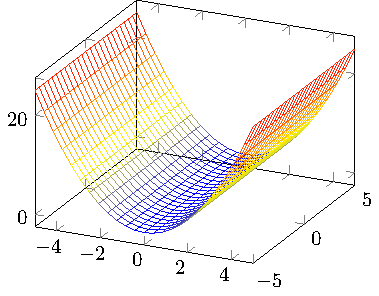
\includegraphics{figures/3Dplot.pdf}
	\caption{A pdf plot}
	\label{Fig pdf of the Distribution of the Sample Correlation Coefficient}
\end{figure}



\newpage
\section{Graphics using .NET Framework}
\label{Tutorial: Graphics}
The mpformulaPy toolbox offers a facility for producing 3D charts. The following pages give a few examples.

\begin{figure}[ht]
	\centering
	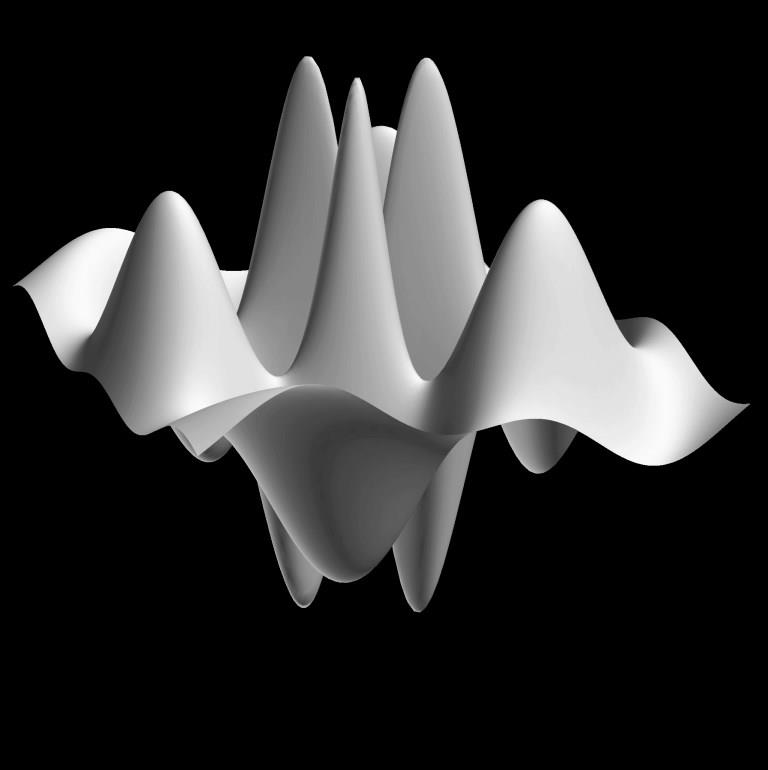
\includegraphics[scale=3.0]{Charts/jpg/SurfaceBlackAndWhite.jpg}
	\caption{plot of a 2-dimensional function}
	\label{Fig plot of a 2-dimensional function}
\end{figure}


The corresponding code is:
\lstset{language={[Sharp]C}}
\begin{lstlisting}
const double two_pi = 2 * Math.PI;
double r2 = x * x + z * z;
double r = Math.Sqrt(r2);
double theta = Math.Atan2(z, x);
result = Math.Exp(-r2) * Math.Sin(two_pi * r) * Math.Cos(3 * theta);
\end{lstlisting}


\newpage
\subsection{Surface plots for bivariate real functions}

The bivariate normal distribution has the following density:
\begin{equation}
	g(x,y;\rho) = \frac{1}{2 \pi \sqrt{1-\rho^2}} e^{\frac{-(x^2 -2\rho x y + y^2)}{2(1-\rho^2)}}
\end{equation}


\begin{figure}[ht]
	\centering
	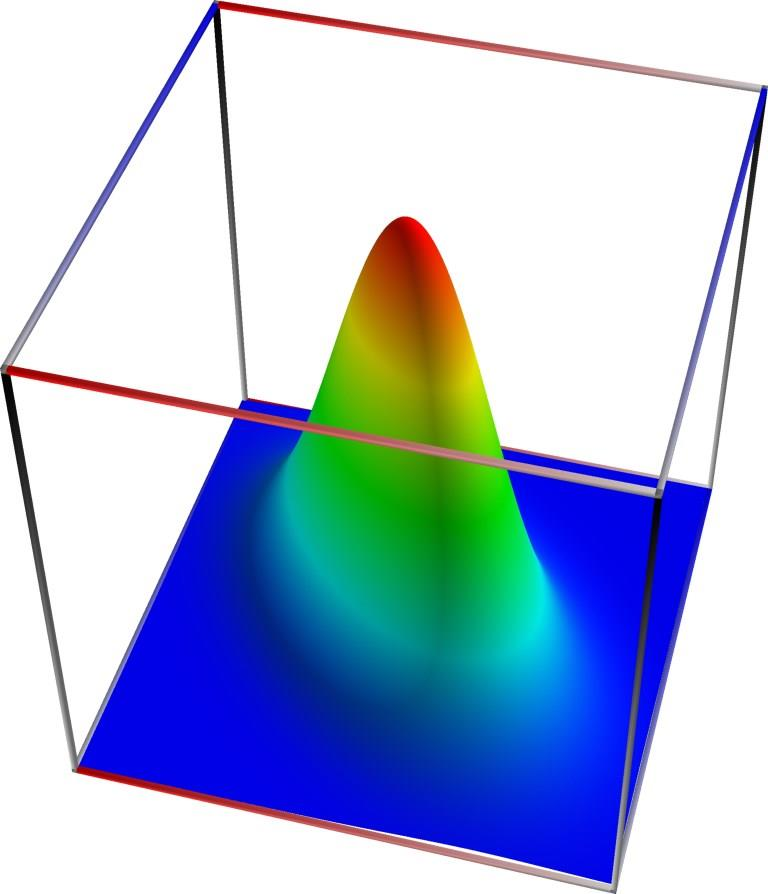
\includegraphics[scale=3.0]{Charts/jpg/BivariateNormal2.jpg}
	\caption{Surface plot of the probability density function of the bivariate normal distribution with $\rho = - 0.5$ }
	\label{Fig plot of the bivariate normal distribution}
\end{figure}


The corresponding code is:
\lstset{language={[Sharp]C}}
\begin{lstlisting}
const double two_pi = 2 * Math.PI;
double rho = -0.5;
double r2 = 1.0 - rho*rho;
double f = 1 / (two_pi * Math.Sqrt(r2));
double e = -(x*x - 2*rho*x*z + z*z)/(2*r2);
result = f * Math.Exp(e);
\end{lstlisting}


\newpage
\subsection{3D Plots of parametric functions}

\subsubsection{3D Plot of a Seashell}

This is a plot of a seashell. 

\begin{figure}[ht]
	\centering
	\includegraphics[scale=3.0]{Charts/jpg/Seashell.jpg}
	\caption[3D plot of a parametric function: Seashell]{3D plot of a parametric function: Seashell. umin = 0; umax = 6*Math.PI; umin = 0; umax = 6*Math.PI. Camera angles are $\theta = 135\degree$ and $\phi = -12\degree$.}
	\label{Fig 3D plot of a parametric function: Seashell}
\end{figure}


The parametrization is:
\lstset{language={[Sharp]C}}
\begin{lstlisting}
double a = Math.Exp(u / (6.0 * Math.PI));
double b = Math.Cos(v / 2.0);

x = 2.0 * (1.0 - a) * Math.Cos(u) * b * b;
z = 2.0 * (-1.0 + a) * Math.Sin(u) * b * b;
y = 1.0 - a * a - Math.Sin(v) * (1.0 - a);
\end{lstlisting}



\newpage
\subsubsection{3D Plot of Kuen's surface}

This is a plot of Kuen's surface. 

\begin{figure}[ht]
	\centering
	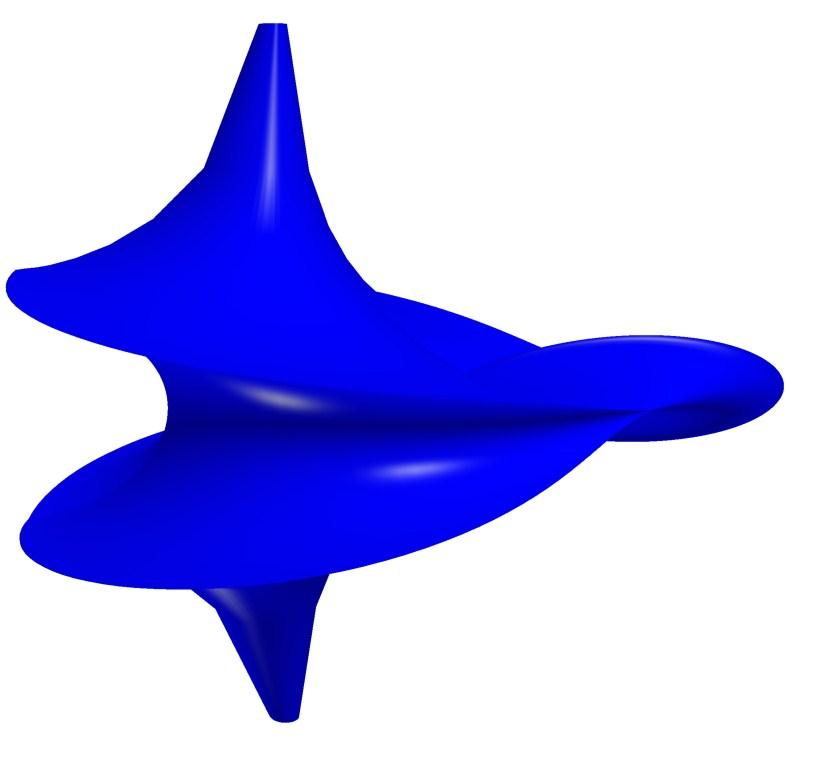
\includegraphics[scale=3.0]{Charts/jpg/KuenSurface.jpg}
	\caption[3D plot of Kuen's surface]{3D plot of a parametric function: Kuen's surface. umin = -4.5; umax = 4.5; vmin = 0.01; vmax = 3.14. Camera angles are $\theta = 135\degree$ and $\phi = -12\degree$.}
	\label{Fig 3D plot of a parametric function: Kuen's surface}
\end{figure}


The parametrization is:
\lstset{language={[Sharp]C}}
\begin{lstlisting}
double a = 1.0 * Math.Sin(v);
double b = 1.0 + u * u * a * a;

x = 2.0 * a * (Math.Cos(u) + u * Math.Sin(u)) / b;
z = 2.0 * a * (Math.Sin(u) - u * Math.Cos(u)) / b;
y = Math.Log(Math.Tan(v/2.0)) + 2.0 * Math.Cos(v) / b;
\end{lstlisting}



\newpage
\subsubsection{3D Plot of Klein's Bottle}

This is a plot of Klein's Bottle. 

\begin{figure}[ht]
	\centering
	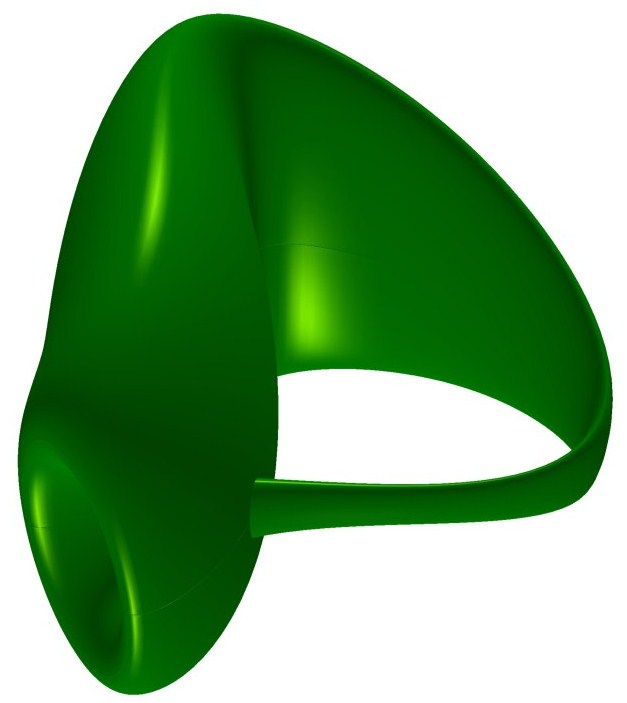
\includegraphics[scale=3.0]{Charts/jpg/KleinBottle.jpg}
	\caption[3D plot of Klein's Bottle]{3D plot of a parametric function: Klein's Bottle. umin = 0.0; umax = 3.14; vmin = 0.0; vmax = 6.28. Camera angles are $\theta = 135\degree$ and $\phi = -12\degree$.}
	\label{Fig 3D plot of a parametric function: Klein's Bottle}
\end{figure}


The following parametrization is due to Robert Israel (with some rearrangements):
\lstset{language={[Sharp]C}}
\begin{lstlisting}
double a = Math.Cos(u);
double b = Math.Sin(u);
double c = Math.Cos(v);
double a2 = a * a;
double a4 = a2 * a2;

x = -(2.0/15.0) * a * (3*c + b*(-30 + a4*(90 - 60*a2) + 5*a*c));
z = -(1.0/15.0) * b*b * (c*b* (3 - 48*a4  + 5*a*b*(1 - 16*a4)) - 60);
y = (2.0/15.0) * (3 + 5*a*b) * Math.Sin(v);
\end{lstlisting}





\newpage
\subsection{Surface plots of complex functions}
\label{Graphics: Surface plots of complex functions}
It is straight forward to produce surface plots of complex functions; these are available in two forms:

\vpara
As plots of the real and imaginary component:

\begin{figure}[ht]
	\centering
	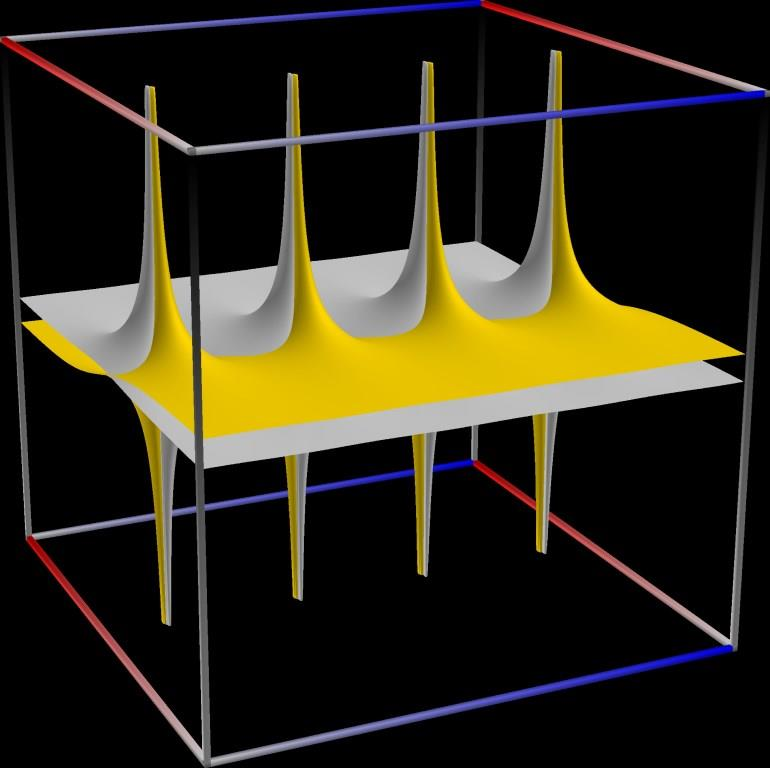
\includegraphics[scale=3.0]{Charts/jpg/ComplexSurfacePlotRealAndImaginary.jpg}
	\caption[Surface plot of the real and imaginary component of $z = \tan(x + iy)$]{Surface plot of the real ("silver") and imaginary ("gold") component of $z = \tan(x + iy)$, $-3 \leq x \leq 3$ (blue axis), $-2 \pi \leq y \leq 2\pi$ (red axis), $-10 \leq z \leq 10$ (black axis). $z$ values are truncated at $\pm 10$. There is a branch cut along the negative real axis. Camera angles are $\theta = 135\degree$ and $\phi = -12\degree$.}
	\label{Fig plot of the re and im of complex tangent}
\end{figure}



%\subsection{Pretty Formatting (specify extra digits)}

\newpage
%\subsection{File Output}
As plots of the absolute value with the phase color-coded:


\begin{figure}[ht]
	\centering
	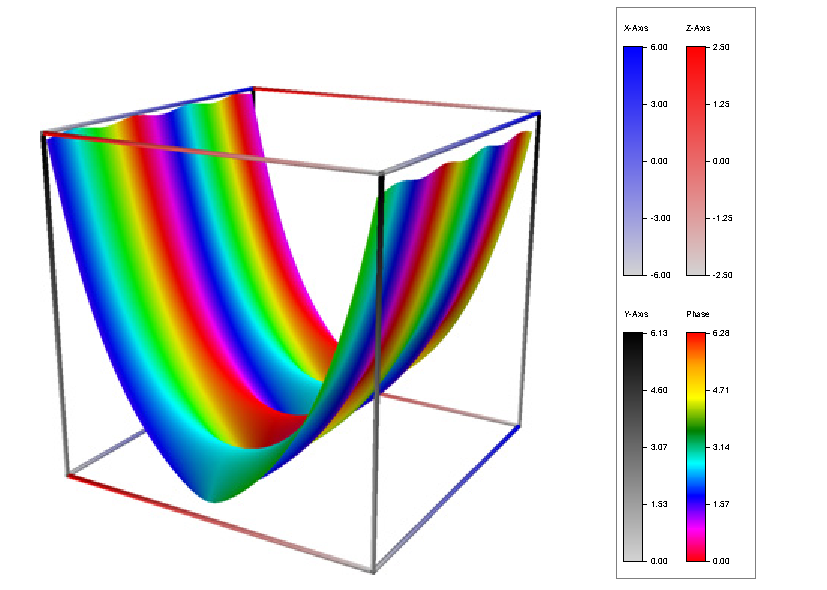
\includegraphics[scale=1.2]{Charts/pdf/SurfacePlotWithScales.pdf}
	\caption[Surface plot of the magnitude of $z = \sin(x + iy)$]{Surface plot of the magnitude and phase (color-coded) of $z = \sin(x + iy)$, $-3 \leq x \leq 3$ (blue axis), $-2 \pi \leq y \leq 2\pi$ (red axis), $-10 \leq z \leq 10$ (black axis). $z$ values are truncated at $\pm 10$. There is a branch cut along the negative real axis. Camera angles are $\theta = 135\degree$ and $\phi = -12\degree$. } 
	\label{Fig plot of the magnitude of complex sine}
\end{figure}




%
%
%\newpage
%\section{Eval, Options, Tables and Charts}
%
%The following functions provide quick access to function evaluations and charts:
%
%\vspace{0.3cm}
%\begin{mpFunctionsExtract}
%	\mpFunctionOne
%	{Eval? String?  the result of the evaluation of an arithmetic expression, containing number and functions, but no variables.}
%	{Expression? String? an arithmetic expression.}
%\end{mpFunctionsExtract}
%
%
%\vspace{0.3cm}
%\begin{mpFunctionsExtract}
%	\mpFunctionOne
%	{Options? String?  an identifier for a set of calculation options.}
%	{BaseOptions? String? an identifier for a set of base calculation options.}
%\end{mpFunctionsExtract}
%
%
%\vspace{0.3cm}
%\begin{mpFunctionsExtract}
%	\mpFunctionOne
%	{Table? Range?  an identifier for a set of calculation options.}
%	{TableRef? String? a reference for a table.}
%\end{mpFunctionsExtract}
%
%
%\vspace{0.3cm}
%\begin{mpFunctionsExtract}
%	\mpFunctionOne
%	{Chart? String?  an identifier for an XML Chart.}
%	{Data? Range? a reference for a data table.}
%\end{mpFunctionsExtract}
%
%


\chapter{Python: Built-in numerical types}


The following sections describe the standard types that are built into the interpreter.

The principal built-in types are numerics, sequences, mappings, classes, instances and exceptions.

Some collection classes are mutable. The methods that add, subtract, or rearrange their members in place, and do not return a specific item, never return the collection instance itself but None.

Some operations are supported by several object types; in particular, practically all objects can be compared, tested for truth value, and converted to a string (with the repr() function or the slightly different str() function). The latter function is implicitly used when an object is written by the print() function.

\section{Truth Value Testing}

Any object can be tested for truth value, for use in an if or while condition or as operand of the Boolean operations below. The following values are considered false:

\vpara
None

False

zero of any numeric type, for example, \verb| 0, 0.0, 0j|.

any empty sequence, for example, \verb| '', (), []|.

any empty mapping, for example, \verb| {}|.

instances of user-defined classes, if the class defines a \_\_bool\_\_() or \_\_len\_\_() method, when that method returns the integer zero or bool value False.

\vpara
All other values are considered true $-$ so objects of many types are always true.

Operations and built-in functions that have a Boolean result always return 0 or False for false and 1 or True for true, unless otherwise stated. (Important exception: the Boolean operations or and and always return one of their operands.)

\section{Boolean Operations:  and, or, not}

These are the Boolean operations, ordered by ascending priority:



\begin{table}[ht]
	\centering
	\begin{tabular}{|l|l|l|}
		\hline
		Operation & Result & Notes\\
		\hline
		\verb|x or y| & if x is false, then y, else x &  (1) \\
		\verb|x and y| & if x is false, then x, else y & (2)  \\
		\verb|not x| & if x is false, then True, else False & (3)  \\								
		\hline
	\end{tabular}
	%	\caption{\result}
	%	\label{\result} 
\end{table}


  

Notes:
1.This is a short-circuit operator, so it only evaluates the second argument if the first one is False.
2.This is a short-circuit operator, so it only evaluates the second argument if the first one is True.
3.not has a lower priority than non-Boolean operators, so not a == b is interpreted as not (a == b), and a == not b is a syntax error.

\section{Comparisons}

There are eight comparison operations in Python. They all have the same priority (which is higher than that of the Boolean operations). Comparisons can be chained arbitrarily; for example, x < y <= z is equivalent to x < y and y <= z, except that y is evaluated only once (but in both cases z is not evaluated at all when x < y is found to be false).

This table summarizes the comparison operations:


\begin{table}[ht]
	\centering
	\begin{tabular}{|l|l|}
		\hline
		Operation & Meaning \\
		\hline
		\verb|<| & strictly less than \\
		\verb|<=| & less than or equal  \\							
		\verb|>| & strictly greater than \\
		\verb|>=| & greater than or equal  \\							
		\verb|==| & equal \\
		\verb|!=| & not equal  \\							
		\verb|is| & object identity \\
		\verb|is not| & negated object identity  \\							
		\hline
	\end{tabular}
	%	\caption{\result}
	%	\label{\result} 
\end{table}


Objects of different types, except different numeric types, never compare equal. Furthermore, some types (for example, function objects) support only a degenerate notion of comparison where any two objects of that type are unequal. The <, <=, > and >= operators will raise a TypeError exception when comparing a complex number with another built-in numeric type, when the objects are of different types that cannot be compared, or in other cases where there is no defined ordering.

Non-identical instances of a class normally compare as non-equal unless the class defines the \_\_eq\_\_() method.

Instances of a class cannot be ordered with respect to other instances of the same class, or other types of object, unless the class defines enough of the methods \_\_lt\_\_(), \_\_le\_\_(), \_\_gt\_\_(), and \_\_ge\_\_() (in general, \_\_lt\_\_() and \_\_eq\_\_() are sufficient, if you want the conventional meanings of the comparison operators).

The behavior of the is and is not operators cannot be customized; also they can be applied to any two objects and never raise an exception.

Two more operations with the same syntactic priority, in and not in, are supported only by sequence types (below).


\section{Numeric Types - int, float, complex}

There are three distinct numeric types: integers, floating point numbers, and complex numbers. In addition, Booleans are a subtype of integers. Integers have unlimited precision. Floating point numbers are usually implemented using double in C; information about the precision and internal representation of floating point numbers for the machine on which your program is running is available in sys.float\_info. Complex numbers have a real and imaginary part, which are each a floating point number. To extract these parts from a complex number z, use z.real and z.imag. (The standard library includes additional numeric types, fractions that hold rationals, and decimal that hold floating-point numbers with user-definable precision.)

\vpara
Numbers are created by numeric literals or as the result of built-in functions and operators. Unadorned integer literals (including hex, octal and binary numbers) yield integers. Numeric literals containing a decimal point or an exponent sign yield floating point numbers. Appending 'j' or 'J' to a numeric literal yields an imaginary number (a complex number with a zero real part) which you can add to an integer or float to get a complex number with real and imaginary parts.

\vpara
Python fully supports mixed arithmetic: when a binary arithmetic operator has operands of different numeric types, the operand with the "narrower" type is widened to that of the other, where integer is narrower than floating point, which is narrower than complex. Comparisons between numbers of mixed type use the same rule. [2] The constructors int(), float(), and complex() can be used to produce numbers of a specific type.

\vpara
All numeric types (except complex) support the following operations, sorted by ascending priority (operations in the same box have the same priority; all numeric operations have a higher priority than comparison operations):


\begin{table}[ht]
	\centering
	\begin{tabular}{|l|l|l|}
		\hline
		Operation & Result & Notes\\
		\hline
		x + y & sum of x and y &   \\
		x - y & difference of x and y &   \\
		x * y & product of x and y &   \\				
		x / y & quotient of x and y &  (1) \\
		x // y & floored quotient of x and y &  \\
		x \% y & remainder of x / y &  (2) \\				
		-x & x negated &   \\
		+x & x unchanged &   \\
		abs(x) & absolute value or magnitude of x &   \\
		int(x) & x converted to integer &  (3)(6) \\
		float(x) & x converted to floating point &  (4)(6) \\
		complex(re, im) & a complex number with real part re, imaginary part im. &  \\
		 & im defaults to zero. &  (6) \\
		c.conjugate() & conjugate of the complex number c &  No \\
		divmod(x, y) & the pair (x // y, x \% y) &  (2) \\
		pow(x, y)  & x to the power y &  (5) \\
		x ** y &  x to the power y &  (5) \\
		math.trunc(x) &  x truncated to Integral &  (7) \\
		round(x[, n]) &  x rounded to n digits, rounding half to even. & \\
		 & If n is omitted, it defaults to 0. &  (7) \\
		math.floor(x) &  the greatest integral float $\le$ x &  (7) \\
		math.ceil(x) &  the least integral float $\ge$ x &  (7) \\
		\hline
	\end{tabular}
	%	\caption{\result}
	%	\label{\result} 
\end{table}
    


Notes:

1.Also referred to as integer division. The resultant value is a whole integer, though the result's type is not necessarily int. The result is always rounded towards minus infinity: 1//2 is 0, (-1)//2 is -1, 1//(-2) is -1, and (-1)//(-2) is 0.

\vpara
2.Not for complex numbers. Instead convert to floats using abs() if appropriate.

\vpara
3.Conversion from floating point to integer may round or truncate as in C; see functions math.floor() and math.ceil() for well-defined conversions.

\vpara
4.float also accepts the strings "nan" and "inf" with an optional prefix "+" or "-" for Not a Number (NaN) and positive or negative infinity.

\vpara
5.Python defines pow(0, 0) and 0 ** 0 to be 1, as is common for programming languages.

\vpara
6.The numeric literals accepted include the digits 0 to 9 or any Unicode equivalent (code points with the Nd property).

7.Only real types (int and float).

See http://www.unicode.org/Public/6.0.0/ucd/extracted/DerivedNumericType.txt for a complete list of code points with the Nd property.


For additional numeric operations see the math and cmath modules.

\section{Long integers}

\subsection{Bitwise Operations on Integer Types}

Bitwise operations only make sense for integers. Negative numbers are treated as their 2’s complement value (this assumes a sufficiently large number of bits that no overflow occurs during the operation).

The priorities of the binary bitwise operations are all lower than the numeric operations and higher than the comparisons; the unary operation ~ has the same priority as the other unary numeric operations (+ and -).

This table lists the bitwise operations sorted in ascending priority (operations in the same box have the same priority):



\begin{table}[ht]
	\centering
	\begin{tabular}{|l|l|l|}
		\hline
		Operation & Result & Notes\\
		\hline
		\verb!x | y! & bitwise or of x and y &   \\
		\verb|x ^ y| & bitwise exclusive or of x and y &   \\
		\verb|x & y| & bitwise and of x and y &   \\				
		\verb|x << n| & x shifted left by n bits & (1)(2) \\
		\verb|x >> n| & x shifted right by n bits & (1)(3) \\
		\verb|~x| & the bits of x inverted &  \\				
		\hline
	\end{tabular}
	%	\caption{\result}
	%	\label{\result} 
\end{table}

    

Notes:
1.Negative shift counts are illegal and cause a ValueError to be raised.
2.A left shift by n bits is equivalent to multiplication by pow(2, n) without overflow check.
3.A right shift by n bits is equivalent to division by pow(2, n) without overflow check.

\subsection{Additional Methods on Integer Types}
 
The int type implements the numbers.Integral abstract base class. In addition, it provides one more method:

\subsubsection{int.bit\_length()}

Return the number of bits necessary to represent an integer in binary, excluding the sign and leading zeros:

\lstset{language={Python}}
\begin{lstlisting}
>>>>>> n = -37
>>> bin(n)
'-0b100101'
>>> n.bit_length()
6
\end{lstlisting}

More precisely, if x is nonzero, then x.bit\_length() is the unique positive integer k such that 2**(k-1) <= abs(x) < 2**k. Equivalently, when abs(x) is small enough to have a correctly rounded logarithm, then k = 1 + int(log(abs(x), 2)). If x is zero, then x.bit\_length() returns 0.

Equivalent to:

\lstset{language={Python}}
\begin{lstlisting}
def bit_length(self):
s = bin(self)       # binary representation:  bin(-37) --> '-0b100101'
s = s.lstrip('-0b') # remove leading zeros and minus sign
return len(s)       # len('100101') --> 6
\end{lstlisting}


\subsubsection{int.to\_bytes}
New in version 3.1.

int.to\_bytes(length, byteorder, *, signed=False)
Return an array of bytes representing an integer.

\lstset{language={Python}}
\begin{lstlisting}
>>>>>> (1024).to_bytes(2, byteorder='big')
b'\x04\x00'
>>> (1024).to_bytes(10, byteorder='big')
b'\x00\x00\x00\x00\x00\x00\x00\x00\x04\x00'
>>> (-1024).to_bytes(10, byteorder='big', signed=True)
b'\xff\xff\xff\xff\xff\xff\xff\xff\xfc\x00'
>>> x = 1000
>>> x.to_bytes((x.bit_length() // 8) + 1, byteorder='little')
b'\xe8\x03'
\end{lstlisting}

The integer is represented using length bytes. An OverflowError is raised if the integer is not representable with the given number of bytes.

The byteorder argument determines the byte order used to represent the integer. If byteorder is "big", the most significant byte is at the beginning of the byte array. If byteorder is "little", the most significant byte is at the end of the byte array. To request the native byte order of the host system, use sys.byteorder as the byte order value.

The signed argument determines whether two’s complement is used to represent the integer. If signed is False and a negative integer is given, an OverflowError is raised. The default value for signed is False.

\subsubsection{int.from\_bytes}
New in version 3.2.

classmethod int.from\_bytes(bytes, byteorder, *, signed=False)
Return the integer represented by the given array of bytes.

\lstset{language={Python}}
\begin{lstlisting}
>>>>>> int.from_bytes(b'\x00\x10', byteorder='big')
16
>>> int.from_bytes(b'\x00\x10', byteorder='little')
4096
>>> int.from_bytes(b'\xfc\x00', byteorder='big', signed=True)
-1024
>>> int.from_bytes(b'\xfc\x00', byteorder='big', signed=False)
64512
>>> int.from_bytes([255, 0, 0], byteorder='big')
16711680
\end{lstlisting}

The argument bytes must either be a bytes-like object or an iterable producing bytes.

The byteorder argument determines the byte order used to represent the integer. If byteorder is "big", the most significant byte is at the beginning of the byte array. If byteorder is "little", the most significant byte is at the end of the byte array. To request the native byte order of the host system, use sys.byteorder as the byte order value.

The signed argument indicates whether two’s complement is used to represent the integer.


\subsection{Additional Methods on Float}

The float type implements the numbers.Real abstract base class. float also has the following additional methods.

\subsubsection{float.as\_integer\_ratio()}

Return a pair of integers whose ratio is exactly equal to the original float and with a positive denominator. Raises OverflowError on infinities and a ValueError on NaNs.

\subsubsection{float.is\_integer()}

Return True if the float instance is finite with integral value, and False otherwise:

\lstset{language={Python}}
\begin{lstlisting}
>>>>>> (-2.0).is_integer()
True
>>> (3.2).is_integer()
False
\end{lstlisting}

Two methods support conversion to and from hexadecimal strings. Since Python's floats are stored internally as binary numbers, converting a float to or from a decimal string usually involves a small rounding error. In contrast, hexadecimal strings allow exact representation and specification of floating-point numbers. This can be useful when debugging, and in numerical work.

\subsubsection{float.hex()}

Return a representation of a floating-point number as a hexadecimal string. For finite floating-point numbers, this representation will always include a leading 0x and a trailing p and exponent.

\subsubsection{float.fromhex(s)}

Class method to return the float represented by a hexadecimal string s. The string s may have leading and trailing whitespace.

\vpara
Note that float.hex() is an instance method, while float.fromhex() is a class method.

A hexadecimal string takes the form:

[sign] ['0x'] integer ['.' fraction] ['p' exponent]

where the optional sign may by either + or -, integer and fraction are strings of hexadecimal digits, and exponent is a decimal integer with an optional leading sign. Case is not significant, and there must be at least one hexadecimal digit in either the integer or the fraction. This syntax is similar to the syntax specified in section 6.4.4.2 of the C99 standard, and also to the syntax used in Java 1.5 onwards. In particular, the output of float.hex() is usable as a hexadecimal floating-point literal in C or Java code, and hexadecimal strings produced by C's \%a format character or Java's Double.toHexString are accepted by float.fromhex().

\vpara
Note that the exponent is written in decimal rather than hexadecimal, and that it gives the power of 2 by which to multiply the coefficient. For example, the hexadecimal string 0x3.a7p10 represents the floating-point number (3 + 10./16 + 7./16**2) * 2.0**10, or 3740.0:

\lstset{language={Python}}
\begin{lstlisting}
>>>>>> float.fromhex('0x3.a7p10')
3740.0
\end{lstlisting}

Applying the reverse conversion to 3740.0 gives a different hexadecimal string representing the same number:

\lstset{language={Python}}
\begin{lstlisting}
>>>>>> float.hex(3740.0)
'0x1.d380000000000p+11'
\end{lstlisting}


\newpage
\section{Fractions}
The fractions module provides support for rational number arithmetic.

A Fraction instance can be constructed from a pair of integers, from another rational number, or from a string.

\vpara
class fractions.Fraction(numerator=0, denominator=1)

class fractions.Fraction(other\_fraction)

class fractions.Fraction(float)

class fractions.Fraction(decimal)

class fractions.Fraction(string)

\vpara
The first version requires that numerator and denominator are instances of numbers.Rational and returns a new Fraction instance with value numerator/denominator. If denominator is 0, it raises a ZeroDivisionError. 

\vpara
The second version requires that other\_fraction is an instance of numbers.Rational and returns a Fraction instance with the same value. 

\vpara
The next two versions accept either a float or a decimal.Decimal instance, and return a Fraction instance with exactly the same value. Note that due to the usual issues with binary floating-point (see Floating Point Arithmetic: Issues and Limitations), the argument to Fraction(1.1) is not exactly equal to 11/10, and so Fraction(1.1) does not return Fraction(11, 10) as one might expect. (But see the documentation for the limit\_denominator() method below.) 

\vpara
The last version of the constructor expects a string or unicode instance. The usual form for this instance is:


[sign] numerator ['/' denominator]


where the optional sign may be either '+' or '-' and numerator and denominator (if present) are strings of decimal digits. In addition, any string that represents a finite value and is accepted by the float constructor is also accepted by the Fraction constructor. In either form the input string may also have leading and/or trailing whitespace. Here are some examples:


\vpara
The corresponding code is:

\lstset{language={Python}}
\begin{lstlisting}
>>>>>> from fractions import Fraction
>>> Fraction(16, -10)
Fraction(-8, 5)
>>> Fraction(123)
Fraction(123, 1)
>>> Fraction()
Fraction(0, 1)
>>> Fraction('3/7')
Fraction(3, 7)
>>> Fraction(' -3/7 ')
Fraction(-3, 7)
>>> Fraction('1.414213 \t\n')
Fraction(1414213, 1000000)
>>> Fraction('-.125')
Fraction(-1, 8)
>>> Fraction('7e-6')
Fraction(7, 1000000)
>>> Fraction(2.25)
Fraction(9, 4)
>>> Fraction(1.1)
Fraction(2476979795053773, 2251799813685248)
>>> from decimal import Decimal
>>> Fraction(Decimal('1.1'))
Fraction(11, 10)
\end{lstlisting}

The Fraction class inherits from the abstract base class numbers.Rational, and implements all of the methods and operations from that class. Fraction instances are hashable, and should be treated as immutable. In addition, Fraction has the following properties and methods:


Changed in version 3.2: The Fraction constructor now accepts float and decimal.Decimal instances.

\subsection{Properties}

\subsubsection{numerator}

Numerator of the Fraction in lowest term.

\subsubsection{denominator}

Denominator of the Fraction in lowest term.

\subsection{Methods}

\subsubsection{from\_float(flt)}

This class method constructs a Fraction representing the exact value of flt, which must be a float. Beware that Fraction.from\_float(0.3) is not the same value as Fraction(3, 10)

Note:
From Python 3.2 onwards, you can also construct a Fraction instance directly from a float.


\subsubsection{from\_decimal(dec)}

This class method constructs a Fraction representing the exact value of dec, which must be a decimal.Decimal instance.

Note:
From Python 3.2 onwards, you can also construct a Fraction instance directly from a decimal.Decimal instance.

\subsubsection{limit\_denominator()}

limit\_denominator(max\_denominator=1000000)
Finds and returns the closest Fraction to self that has denominator at most max\_denominator. This method is useful for finding rational approximations to a given floating-point number:

\lstset{language={Python}}
\begin{lstlisting}
>>>>>> from fractions import Fraction
>>> Fraction('3.1415926535897932').limit\_denominator(1000)
Fraction(355, 113)
\end{lstlisting}

or for recovering a rational number that’s represented as a float:

\lstset{language={Python}}
\begin{lstlisting}
>>>>>> from math import pi, cos
>>> Fraction(cos(pi/3))
Fraction(4503599627370497, 9007199254740992)
>>> Fraction(cos(pi/3)).limit\_denominator()
Fraction(1, 2)
>>> Fraction(1.1).limit\_denominator()
Fraction(11, 10)
\end{lstlisting}

\subsubsection{\_\_floor\_\_()}

Returns the greatest int <= self. This method can also be accessed through the math.floor() function:

\lstset{language={Python}}
\begin{lstlisting}
>>>>>> from math import floor
>>> floor(Fraction(355, 113))
3
\end{lstlisting}

\subsubsection{\_\_ceil\_\_()}

Returns the least int >= self. This method can also be accessed through the math.ceil() function.

\subsubsection{\_\_round\_\_()}

\textbf{\_\_round\_\_()}

\textbf{\_\_round\_\_(ndigits)}

The first version returns the nearest int to self, rounding half to even. The second version rounds self to the nearest multiple of Fraction(1, 10**ndigits) (logically, if ndigits is negative), again rounding half toward even. This method can also be accessed through the round() function.

\subsubsection{fractions.gcd(a, b)}

Return the greatest common divisor of the integers a and b. If either a or b is nonzero, then the absolute value of gcd(a, b) is the largest integer that divides both a and b. gcd(a,b) has the same sign as b if b is nonzero; otherwise it takes the sign of a. gcd(0, 0) returns 0.










%
%
%
%
%\newpage
%\section{Decimals}
%
%\subsection{Overview}
%
%The decimal module provides support for fast correctly-rounded decimal floating point arithmetic. It offers several advantages over the float datatype:
%
%\vpara
%Decimal "is based on a floating-point model which was designed with people in mind, and necessarily has a paramount guiding principle $-$ computers must provide an arithmetic that works in the same way as the arithmetic that people learn at school." $-$ excerpt from the decimal arithmetic specification.
%
%\vpara
%Decimal numbers can be represented exactly. In contrast, numbers like 1.1 and 2.2 do not have exact representations in binary floating point. End users typically would not expect 1.1 + 2.2 to display as 3.3000000000000003 as it does with binary floating point.
%
%\vpara
%The exactness carries over into arithmetic. In decimal floating point, 0.1 + 0.1 + 0.1 - 0.3 is exactly equal to zero. In binary floating point, the result is 5.5511151231257827e-017. While near to zero, the differences prevent reliable equality testing and differences can accumulate. For this reason, decimal is preferred in accounting applications which have strict equality invariants.
%
%\vpara
%The decimal module incorporates a notion of significant places so that 1.30 + 1.20 is 2.50. The trailing zero is kept to indicate significance. This is the customary presentation for monetary applications. For multiplication, the "schoolbook" approach uses all the figures in the multiplicands. For instance, 1.3 * 1.2 gives 1.56 while 1.30 * 1.20 gives 1.5600.
%
%\vpara
%Unlike hardware based binary floating point, the decimal module has a user alterable precision (defaulting to 28 places) which can be as large as needed for a given problem:
%
%\lstset{language={Python}}
%\begin{lstlisting}
%>>> from decimal import *
%>>> getcontext().prec = 6
%>>> Decimal(1) / Decimal(7)
%Decimal('0.142857')
%>>> getcontext().prec = 28
%>>> Decimal(1) / Decimal(7)
%Decimal('0.1428571428571428571428571429')
%\end{lstlisting}
%
%
%Both binary and decimal floating point are implemented in terms of published standards. While the built-in float type exposes only a modest portion of its capabilities, the decimal module exposes all required parts of the standard. When needed, the programmer has full control over rounding and signal handling. This includes an option to enforce exact arithmetic by using exceptions to block any inexact operations.
%
%\vpara
%The decimal module was designed to support "without prejudice, both exact unrounded decimal arithmetic (sometimes called fixed-point arithmetic) and rounded floating-point arithmetic." $-$ excerpt from the decimal arithmetic specification.
%
%\vpara
%The module design is centered around three concepts: the decimal number, the context for arithmetic, and signals.
%
%\vpara
%A decimal number is immutable. It has a sign, coefficient digits, and an exponent. To preserve significance, the coefficient digits do not truncate trailing zeros. Decimals also include special values such as Infinity, -Infinity, and NaN. The standard also differentiates -0 from +0.
%
%\vpara
%The context for arithmetic is an environment specifying precision, rounding rules, limits on exponents, flags indicating the results of operations, and trap enablers which determine whether signals are treated as exceptions. Rounding options include ROUND\_CEILING, ROUND\_DOWN, ROUND\_FLOOR, ROUND\_HALF\_DOWN, ROUND\_HALF\_EVEN, ROUND\_HALF\_UP, ROUND\_UP, and ROUND\_05UP.
%
%\vpara
%Signals are groups of exceptional conditions arising during the course of computation. Depending on the needs of the application, signals may be ignored, considered as informational, or treated as exceptions. The signals in the decimal module are: Clamped, InvalidOperation, DivisionByZero, Inexact, Rounded, Subnormal, Overflow, Underflow and FloatOperation.
%
%\vpara
%For each signal there is a flag and a trap enabler. When a signal is encountered, its flag is set to one, then, if the trap enabler is set to one, an exception is raised. Flags are sticky, so the user needs to reset them before monitoring a calculation.
%
%\vpara
%See also:
%
%IBM's General Decimal Arithmetic Specification, The General Decimal Arithmetic Specification.
%
%IEEE standard 854-1987, Unofficial IEEE 854 Text.
%
%
%
%\subsection{Quick-start Tutorial}
%
%The usual start to using decimals is importing the module, viewing the current context with getcontext() and, if necessary, setting new values for precision, rounding, or enabled traps:
%
%\lstset{language={Python}}
%\begin{lstlisting}
%>>> from decimal import *
%>>> getcontext()
%Context(prec=28, rounding=ROUND\_HALF\_EVEN, Emin=-999999, Emax=999999,
%capitals=1, clamp=0, flags=[], traps=[Overflow, DivisionByZero, 
%InvalidOperation])
%
%>>> getcontext().prec = 7       # Set a new precision
%\end{lstlisting}
%
%Decimal instances can be constructed from integers, strings, floats, or tuples. Construction from an integer or a float performs an exact conversion of the value of that integer or float. Decimal numbers include special values such as NaN which stands for “Not a number”, positive and negative Infinity, and -0:
%
%\lstset{language={Python}}
%\begin{lstlisting}
%>>> getcontext().prec = 28
%>>> Decimal(10)
%Decimal('10')
%>>> Decimal('3.14')
%Decimal('3.14')
%>>> Decimal(3.14)
%Decimal('3.140000000000000124344978758017532527446746826171875')
%>>> Decimal((0, (3, 1, 4), -2))
%Decimal('3.14')
%>>> Decimal(str(2.0 ** 0.5))
%Decimal('1.4142135623730951')
%>>> Decimal(2) ** Decimal('0.5')
%Decimal('1.414213562373095048801688724')
%>>> Decimal('NaN')
%Decimal('NaN')
%>>> Decimal('-Infinity')
%Decimal('-Infinity')
%\end{lstlisting}
%
%If the FloatOperation signal is trapped, accidental mixing of decimals and floats in constructors or ordering comparisons raises an exception:
%
%\lstset{language={Python}}
%\begin{lstlisting}
%>>> c = getcontext()
%>>> c.traps[FloatOperation] = True
%>>> Decimal(3.14)
%Traceback (most recent call last):
%File "<stdin>", line 1, in <module>
%decimal.FloatOperation: [<class 'decimal.FloatOperation'>]
%>>> Decimal('3.5') < 3.7
%Traceback (most recent call last):
%File "<stdin>", line 1, in <module>
%decimal.FloatOperation: [<class 'decimal.FloatOperation'>]
%>>> Decimal('3.5') == 3.5
%True
%\end{lstlisting}
%
%New in version 3.3.
%
%The significance of a new Decimal is determined solely by the number of digits input. Context precision and rounding only come into play during arithmetic operations.
%
%\lstset{language={Python}}
%\begin{lstlisting}
%>>> getcontext().prec = 6
%>>> Decimal('3.0')
%Decimal('3.0')
%>>> Decimal('3.1415926535')
%Decimal('3.1415926535')
%>>> Decimal('3.1415926535') + Decimal('2.7182818285')
%Decimal('5.85987')
%>>> getcontext().rounding = ROUND\_UP
%>>> Decimal('3.1415926535') + Decimal('2.7182818285')
%Decimal('5.85988')
%\end{lstlisting}
%
%If the internal limits of the C version are exceeded, constructing a decimal raises InvalidOperation:
%
%\lstset{language={Python}}
%\begin{lstlisting}
%>>> Decimal("1e9999999999999999999")
%Traceback (most recent call last):
%File "<stdin>", line 1, in <module>
%decimal.InvalidOperation: [<class 'decimal.InvalidOperation'>]
%\end{lstlisting}
%
%
%Changed in version 3.3.
%
%Decimals interact well with much of the rest of Python. Here is a small decimal floating point flying circus:
%
%\lstset{language={Python}}
%\begin{lstlisting}
%>>> data = list(map(Decimal, '1.34 1.87 3.45 2.35 1.00 0.03 9.25'.split()))
%>>> max(data)
%Decimal('9.25')
%>>> min(data)
%Decimal('0.03')
%>>> sorted(data)
%[Decimal('0.03'), Decimal('1.00'), Decimal('1.34'), Decimal('1.87'),
%Decimal('2.35'), Decimal('3.45'), Decimal('9.25')]
%>>> sum(data)
%Decimal('19.29')
%>>> a,b,c = data[:3]
%>>> str(a)
%'1.34'
%>>> float(a)
%1.34
%>>> round(a, 1)
%Decimal('1.3')
%>>> int(a)
%1
%>>> a * 5
%Decimal('6.70')
%>>> a * b
%Decimal('2.5058')
%>>> c % a
%Decimal('0.77')
%\end{lstlisting}
%
%And some mathematical functions are also available to Decimal:
%
%\lstset{language={Python}}
%\begin{lstlisting}
%>>> getcontext().prec = 28
%>>> Decimal(2).sqrt()
%Decimal('1.414213562373095048801688724')
%>>> Decimal(1).exp()
%Decimal('2.718281828459045235360287471')
%>>> Decimal('10').ln()
%Decimal('2.302585092994045684017991455')
%>>> Decimal('10').log10()
%Decimal('1')
%\end{lstlisting}
%
%The quantize() method rounds a number to a fixed exponent. This method is useful for monetary applications that often round results to a fixed number of places:
%
%\lstset{language={Python}}
%\begin{lstlisting}
%>>> Decimal('7.325').quantize(Decimal('.01'), rounding=ROUND\_DOWN)
%Decimal('7.32')
%>>> Decimal('7.325').quantize(Decimal('1.'), rounding=ROUND\_UP)
%Decimal('8')
%\end{lstlisting}
%
%As shown above, the getcontext() function accesses the current context and allows the settings to be changed. This approach meets the needs of most applications.
%
%For more advanced work, it may be useful to create alternate contexts using the Context() constructor. To make an alternate active, use the setcontext() function.
%
%In accordance with the standard, the Decimal module provides two ready to use standard contexts, BasicContext and ExtendedContext. The former is especially useful for debugging because many of the traps are enabled:
%
%\lstset{language={Python}}
%\begin{lstlisting}
%>>> myothercontext = Context(prec=60, rounding=ROUND\_HALF\_DOWN)
%>>> setcontext(myothercontext)
%>>> Decimal(1) / Decimal(7)
%Decimal('0.142857142857142857142857142857142857142857142857142857142857')
%
%>>> ExtendedContext
%Context(prec=9, rounding=ROUND\_HALF\_EVEN, Emin=-999999, Emax=999999,
%capitals=1, clamp=0, flags=[], traps=[])
%>>> setcontext(ExtendedContext)
%>>> Decimal(1) / Decimal(7)
%Decimal('0.142857143')
%>>> Decimal(42) / Decimal(0)
%Decimal('Infinity')
%
%>>> setcontext(BasicContext)
%>>> Decimal(42) / Decimal(0)
%Traceback (most recent call last):
%File "<pyshell#143>", line 1, in -toplevel-
%Decimal(42) / Decimal(0)
%DivisionByZero: x / 0
%\end{lstlisting}
%
%Contexts also have signal flags for monitoring exceptional conditions encountered during computations. The flags remain set until explicitly cleared, so it is best to clear the flags before each set of monitored computations by using the clear\_flags() method.
%
%\lstset{language={Python}}
%\begin{lstlisting}
%>>> setcontext(ExtendedContext)
%>>> getcontext().clear\_flags()
%>>> Decimal(355) / Decimal(113)
%Decimal('3.14159292')
%>>> getcontext()
%Context(prec=9, rounding=ROUND\_HALF\_EVEN, Emin=-999999, Emax=999999,
%capitals=1, clamp=0, flags=[Inexact, Rounded], traps=[])
%\end{lstlisting}
%
%The flags entry shows that the rational approximation to Pi was rounded (digits beyond the context precision were thrown away) and that the result is inexact (some of the discarded digits were non-zero).
%
%Individual traps are set using the dictionary in the traps field of a context:
%
%\lstset{language={Python}}
%\begin{lstlisting}
%>>> setcontext(ExtendedContext)
%>>> Decimal(1) / Decimal(0)
%Decimal('Infinity')
%>>> getcontext().traps[DivisionByZero] = 1
%>>> Decimal(1) / Decimal(0)
%Traceback (most recent call last):
%File "<pyshell#112>", line 1, in -toplevel-
%Decimal(1) / Decimal(0)
%DivisionByZero: x / 0
%\end{lstlisting}
%
%Most programs adjust the current context only once, at the beginning of the program. And, in many applications, data is converted to Decimal with a single cast inside a loop. With context set and decimals created, the bulk of the program manipulates the data no differently than with other Python numeric types.
%
%
%
%\subsection{Decimal objects}
%
%class decimal.Decimal(value="0", context=None)
%
%Construct a new Decimal object based from value.
%
%value can be an integer, string, tuple, float, or another Decimal object. If no value is given, returns Decimal('0'). If value is a string, it should conform to the decimal numeric string syntax after leading and trailing whitespace characters are removed:
%
%\lstset{language={Python}}
%\begin{lstlisting}
%sign           ::=  '+' | '-'
%digit          ::=  '0' | '1' | '2' | '3' | '4' | '5' | '6' | '7' | '8' | '9'
%indicator      ::=  'e' | 'E'
%digits         ::=  digit [digit]...
%decimal-part   ::=  digits '.' [digits] | ['.'] digits
%exponent-part  ::=  indicator [sign] digits
%infinity       ::=  'Infinity' | 'Inf'
%nan            ::=  'NaN' [digits] | 'sNaN' [digits]
%numeric-value  ::=  decimal-part [exponent-part] | infinity
%numeric-string ::=  [sign] numeric-value | [sign] nan
%\end{lstlisting}
%
%Other Unicode decimal digits are also permitted where digit appears above. These include decimal digits from various other alphabets (for example, Arabic-Indic and Devanagari digits) along with the fullwidth digits '\\uff10' through '\\uff19'.
%
%\vpara
%If value is a tuple, it should have three components, a sign (0 for positive or 1 for negative), a tuple of digits, and an integer exponent. For example, Decimal((0, (1, 4, 1, 4), -3)) returns Decimal('1.414').
%
%\vpara
%If value is a float, the binary floating point value is losslessly converted to its exact decimal equivalent. This conversion can often require 53 or more digits of precision. For example,
%
%Decimal(float('1.1')) converts to 
%
%Decimal('1.100000000000000088817841970012523233890533447265625').
%
%\vpara
%The context precision does not affect how many digits are stored. That is determined exclusively by the number of digits in value. For example, Decimal('3.00000') records all five zeros even if the context precision is only three.
%
%\vpara
%The purpose of the context argument is determining what to do if value is a malformed string. If the context traps InvalidOperation, an exception is raised; otherwise, the constructor returns a new Decimal with the value of NaN.
%
%\vpara
%Once constructed, Decimal objects are immutable.
%
%Changed in version 3.2: The argument to the constructor is now permitted to be a float instance.
%
%Changed in version 3.3: float arguments raise an exception if the FloatOperation trap is set. By default the trap is off.
%
%\vpara
%Decimal floating point objects share many properties with the other built-in numeric types such as float and int. All of the usual math operations and special methods apply. Likewise, decimal objects can be copied, pickled, printed, used as dictionary keys, used as set elements, compared, sorted, and coerced to another type (such as float or int).
%
%\vpara
%There are some small differences between arithmetic on Decimal objects and arithmetic on integers and floats. When the remainder operator \% is applied to Decimal objects, the sign of the result is the sign of the dividend rather than the sign of the divisor:
%
%\lstset{language={Python}}
%\begin{lstlisting}
%>>> (-7) % 4
%1
%>>> Decimal(-7) % Decimal(4)
%Decimal('-3')
%\end{lstlisting}
%
%The integer division operator // behaves analogously, returning the integer part of the true quotient (truncating towards zero) rather than its floor, so as to preserve the usual identity 
%
%x == (x // y) * y + x % y:
%
%\lstset{language={Python}}
%\begin{lstlisting}
%>>> -7 // 4
%-2
%>>> Decimal(-7) // Decimal(4)
%Decimal('-1')
%\end{lstlisting}
%
%The \% and // operators implement the remainder and divide-integer operations (respectively) as described in the specification.
%
%\vpara
%Decimal objects cannot generally be combined with floats or instances of fractions.Fraction in arithmetic operations: an attempt to add a Decimal to a float, for example, will raise a TypeError. However, it is possible to use Python's comparison operators to compare a Decimal instance x with another number y. This avoids confusing results when doing equality comparisons between numbers of different types.
%
%
%Changed in version 3.2: Mixed-type comparisons between Decimal instances and other numeric types are now fully supported.
%
%
%
%\subsection{Methods}
%In addition to the standard numeric properties, decimal floating point objects also have a number of specialized methods:
%
%\subsubsection{adjusted()}
%
%Return the adjusted exponent after shifting out the coefficient’s rightmost digits until only the lead digit remains: Decimal('321e+5').adjusted() returns seven. Used for determining the position of the most significant digit with respect to the decimal point.
%
%\subsubsection{as\_tuple()}
%
%Return a named tuple representation of the number: DecimalTuple(sign, digits, exponent).
%
%\subsubsection{canonical()}
%
%Return the canonical encoding of the argument. Currently, the encoding of a Decimal instance is always canonical, so this operation returns its argument unchanged.
%
%\subsubsection{compare(other, context=None)}
%
%Compare the values of two Decimal instances. compare() returns a Decimal instance, and if either operand is a NaN then the result is a NaN:
%
%\lstset{language={Python}}
%\begin{lstlisting}
%a or b is a NaN  ==> Decimal('NaN')
%a < b            ==> Decimal('-1')
%a == b           ==> Decimal('0')
%a > b            ==> Decimal('1')
%\end{lstlisting}
%
%\subsubsection{compare\_signal(other, context=None)}
%
%This operation is identical to the compare() method, except that all NaNs signal. That is, if neither operand is a signaling NaN then any quiet NaN operand is treated as though it were a signaling NaN.
%
%\subsubsection{compare\_total(other, context=None)}
%
%Compare two operands using their abstract representation rather than their numerical value. Similar to the compare() method, but the result gives a total ordering on Decimal instances. Two Decimal instances with the same numeric value but different representations compare unequal in this ordering:
%
%\lstset{language={Python}}
%\begin{lstlisting}
%>>> Decimal('12.0').compare\_total(Decimal('12'))
%Decimal('-1')
%\end{lstlisting}
%
%Quiet and signaling NaNs are also included in the total ordering. The result of this function is Decimal('0') if both operands have the same representation, Decimal('-1') if the first operand is lower in the total order than the second, and Decimal('1') if the first operand is higher in the total order than the second operand. See the specification for details of the total order.
%
%This operation is unaffected by context and is quiet: no flags are changed and no rounding is performed. As an exception, the C version may raise InvalidOperation if the second operand cannot be converted exactly.
%
%\subsubsection{compare\_total\_mag(other, context=None)}
%
%Compare two operands using their abstract representation rather than their value as in compare\_total(), but ignoring the sign of each operand. x.compare\_total\_mag(y) is equivalent to x.copy\_abs().compare\_total(y.copy\_abs()).
%
%This operation is unaffected by context and is quiet: no flags are changed and no rounding is performed. As an exception, the C version may raise InvalidOperation if the second operand cannot be converted exactly.
%
%
%\subsubsection{conjugate()}
%
%Just returns self, this method is only to comply with the Decimal Specification.
%
%
%\subsubsection{copy\_abs()}
%
%Return the absolute value of the argument. This operation is unaffected by the context and is quiet: no flags are changed and no rounding is performed.
%
%
%\subsubsection{copy\_negate()}
%
%Return the negation of the argument. This operation is unaffected by the context and is quiet: no flags are changed and no rounding is performed.
%
%
%\subsubsection{copy\_sign(other, context=None)}
%
%Return a copy of the first operand with the sign set to be the same as the sign of the second operand. For example:
%
%\lstset{language={Python}}
%\begin{lstlisting}
%>>> Decimal('2.3').copy\_sign(Decimal('-1.5'))
%Decimal('-2.3')
%\end{lstlisting}
%
%This operation is unaffected by context and is quiet: no flags are changed and no rounding is performed. As an exception, the C version may raise InvalidOperation if the second operand cannot be converted exactly.
%
%
%\subsubsection{exp(context=None)}
%
%Return the value of the (natural) exponential function e**x at the given number. The result is correctly rounded using the ROUND\_HALF\_EVEN rounding mode.
%
%\lstset{language={Python}}
%\begin{lstlisting}
%>>> Decimal(1).exp()
%Decimal('2.718281828459045235360287471')
%>>> Decimal(321).exp()
%Decimal('2.561702493119680037517373933E+139')
%\end{lstlisting}
%
%\subsubsection{from\_float(f)}
%
%Classmethod that converts a float to a decimal number, exactly.
%
%Note Decimal.from\_float(0.1) is not the same as Decimal('0.1'). Since 0.1 is not exactly representable in binary floating point, the value is stored as the nearest representable value which is 0x1.999999999999ap-4. That equivalent value in decimal is
%
%0.1000000000000000055511151231257827021181583404541015625.
%
%\vpara
%Note:
%From Python 3.2 onwards, a Decimal instance can also be constructed directly from a float.
%
%
%\lstset{language={Python}}
%\begin{lstlisting}
%>>> Decimal.from_float(0.1)
%Decimal('0.1000000000000000055511151231257827021181583404541015625')
%>>> Decimal.from_float(float('nan'))
%Decimal('NaN')
%>>> Decimal.from_float(float('inf'))
%Decimal('Infinity')
%>>> Decimal.from_float(float('-inf'))
%Decimal('-Infinity')
%\end{lstlisting}
%
%
%\subsubsection{fma(other, third, context=None)}
%
%New in version 3.1. 
%
%Fused multiply-add. Return self*other+third with no rounding of the intermediate product self*other.
%
%\lstset{language={Python}}
%\begin{lstlisting}
%>>> Decimal(2).fma(3, 5)
%Decimal('11')
%\end{lstlisting}
%
%\subsubsection{is\_canonical()}
%
%Return True if the argument is canonical and False otherwise. Currently, a Decimal instance is always canonical, so this operation always returns True.
%
%\subsubsection{is\_finite()}
%
%Return True if the argument is a finite number, and False if the argument is an infinity or a NaN.
%
%\subsubsection{is\_infinite()}
%
%Return True if the argument is either positive or negative infinity and False otherwise.
%
%\subsubsection{is\_nan()}
%
%Return True if the argument is a (quiet or signaling) NaN and False otherwise.
%
%\subsubsection{is\_normal(context=None)}
%
%Return True if the argument is a normal finite number. Return False if the argument is zero, subnormal, infinite or a NaN.
%
%\subsubsection{is\_qnan()}
%
%Return True if the argument is a quiet NaN, and False otherwise.
%
%\subsubsection{is\_signed()}
%
%Return True if the argument has a negative sign and False otherwise. Note that zeros and NaNs can both carry signs.
%
%\subsubsection{is\_snan()}
%
%Return True if the argument is a signaling NaN and False otherwise.
%
%\subsubsection{is\_subnormal(context=None)}
%
%Return True if the argument is subnormal, and False otherwise.
%
%\subsubsection{is\_zero()}
%
%Return True if the argument is a (positive or negative) zero and False otherwise.
%
%\subsubsection{ln(context=None)}
%
%Return the natural (base e) logarithm of the operand. The result is correctly rounded using the ROUND\_HALF\_EVEN rounding mode.
%
%\subsubsection{log10(context=None)}
%
%Return the base ten logarithm of the operand. The result is correctly rounded using the ROUND\_HALF\_EVEN rounding mode.
%
%\subsubsection{logb(context=None)}
%
%For a nonzero number, return the adjusted exponent of its operand as a Decimal instance. If the operand is a zero then Decimal('-Infinity') is returned and the DivisionByZero flag is raised. If the operand is an infinity then Decimal('Infinity') is returned.
%
%\subsubsection{logical\_and(other, context=None)}
%
%logical\_and() is a logical operation which takes two logical operands (see Logical operands). The result is the digit-wise and of the two operands.
%
%\subsubsection{logical\_invert(context=None)}
%
%logical\_invert() is a logical operation. The result is the digit-wise inversion of the operand.
%
%
%\subsubsection{logical\_or(other, context=None)}
%
%logical\_or() is a logical operation which takes two logical operands (see Logical operands). The result is the digit-wise or of the two operands.
%
%\subsubsection{logical\_xor(other, context=None)}
%
%logical\_xor() is a logical operation which takes two logical operands (see Logical operands). The result is the digit-wise exclusive or of the two operands.
%
%\subsubsection{max(other, context=None)}
%
%Like max(self, other) except that the context rounding rule is applied before returning and that NaN values are either signaled or ignored (depending on the context and whether they are signaling or quiet).
%
%\subsubsection{max\_mag(other, context=None)}
%
%Similar to the max() method, but the comparison is done using the absolute values of the operands.
%
%\subsubsection{min(other, context=None)}
%
%Like min(self, other) except that the context rounding rule is applied before returning and that NaN values are either signaled or ignored (depending on the context and whether they are signaling or quiet).
%
%\subsubsection{min\_mag(other, context=None)}
%
%Similar to the min() method, but the comparison is done using the absolute values of the operands.
%next\_minus(context=None)
%Return the largest number representable in the given context (or in the current thread’s context if no context is given) that is smaller than the given operand.
%
%\subsubsection{next\_plus(context=None)}
%
%Return the smallest number representable in the given context (or in the current thread’s context if no context is given) that is larger than the given operand.
%
%\subsubsection{next\_toward(other, context=None)}
%
%If the two operands are unequal, return the number closest to the first operand in the direction of the second operand. If both operands are numerically equal, return a copy of the first operand with the sign set to be the same as the sign of the second operand.
%
%\subsubsection{normalize(context=None)}
%
%Normalize the number by stripping the rightmost trailing zeros and converting any result equal to Decimal('0') to Decimal('0e0'). Used for producing canonical values for attributes of an equivalence class. For example, Decimal('32.100') and Decimal('0.321000e+2') both normalize to the equivalent value Decimal('32.1').
%
%\subsubsection{number\_class(context=None)}
%
%Return a string describing the class of the operand. The returned value is one of the following ten strings.
%
%\lstset{language={Python}}
%\begin{lstlisting}
%"-Infinity", indicating that the operand is negative infinity.
%"-Normal", indicating that the operand is a negative normal number.
%"-Subnormal", indicating that the operand is negative and subnormal.
%"-Zero", indicating that the operand is a negative zero.
%"+Zero", indicating that the operand is a positive zero.
%"+Subnormal", indicating that the operand is positive and subnormal.
%"+Normal", indicating that the operand is a positive normal number.
%"+Infinity", indicating that the operand is positive infinity.
%"NaN", indicating that the operand is a quiet NaN (Not a Number).
%"sNaN", indicating that the operand is a signaling NaN.
%\end{lstlisting}
%
%
%\subsubsection{quantize(exp, rounding=None, context=None, watchexp=True)}
%
%Return a value equal to the first operand after rounding and having the exponent of the second operand.
%
%\lstset{language={Python}}
%\begin{lstlisting}
%>>> Decimal('1.41421356').quantize(Decimal('1.000'))
%Decimal('1.414')
%\end{lstlisting}
%
%Unlike other operations, if the length of the coefficient after the quantize operation would be greater than precision, then an InvalidOperation is signaled. This guarantees that, unless there is an error condition, the quantized exponent is always equal to that of the right-hand operand.
%
%Also unlike other operations, quantize never signals Underflow, even if the result is subnormal and inexact.
%
%If the exponent of the second operand is larger than that of the first then rounding may be necessary. In this case, the rounding mode is determined by the rounding argument if given, else by the given context argument; if neither argument is given the rounding mode of the current thread’s context is used.
%
%If watchexp is set (default), then an error is returned whenever the resulting exponent is greater than Emax or less than Etiny.
%
%Deprecated since version 3.3: watchexp is an implementation detail from the pure Python version and is not present in the C version. It will be removed in version 3.4, where it defaults to True.
%
%
%\subsubsection{radix()}
%
%Return Decimal(10), the radix (base) in which the Decimal class does all its arithmetic. Included for compatibility with the specification.
%
%\subsubsection{remainder\_near(other, context=None)}
%
%Return the remainder from dividing self by other. This differs from self \% other in that the sign of the remainder is chosen so as to minimize its absolute value. More precisely, the return value is self - n * other where n is the integer nearest to the exact value of self / other, and if two integers are equally near then the even one is chosen.
%
%If the result is zero then its sign will be the sign of self.
%
%\lstset{language={Python}}
%\begin{lstlisting}
%>>> Decimal(18).remainder\_near(Decimal(10))
%Decimal('-2')
%>>> Decimal(25).remainder\_near(Decimal(10))
%Decimal('5')
%>>> Decimal(35).remainder\_near(Decimal(10))
%Decimal('-5')
%\end{lstlisting}
%
%\subsubsection{rotate(other, context=None)}
%
%Return the result of rotating the digits of the first operand by an amount specified by the second operand. The second operand must be an integer in the range -precision through precision. The absolute value of the second operand gives the number of places to rotate. If the second operand is positive then rotation is to the left; otherwise rotation is to the right. The coefficient of the first operand is padded on the left with zeros to length precision if necessary. The sign and exponent of the first operand are unchanged.
%
%\subsubsection{same\_quantum(other, context=None)}
%
%Test whether self and other have the same exponent or whether both are NaN.
%
%This operation is unaffected by context and is quiet: no flags are changed and no rounding is performed. As an exception, the C version may raise InvalidOperation if the second operand cannot be converted exactly.
%
%\subsubsection{scaleb(other, context=None)}
%
%Return the first operand with exponent adjusted by the second. Equivalently, return the first operand multiplied by 10**other. The second operand must be an integer.
%
%\subsubsection{shift(other, context=None)}
%
%Return the result of shifting the digits of the first operand by an amount specified by the second operand. The second operand must be an integer in the range -precision through precision. The absolute value of the second operand gives the number of places to shift. If the second operand is positive then the shift is to the left; otherwise the shift is to the right. Digits shifted into the coefficient are zeros. The sign and exponent of the first operand are unchanged.
%
%\subsubsection{sqrt(context=None)}
%
%Return the square root of the argument to full precision.
%
%
%\subsubsection{to\_eng\_string(context=None)}
%
%Convert to an engineering-type string.
%
%Engineering notation has an exponent which is a multiple of 3, so there are up to 3 digits left of the decimal place. For example, converts Decimal('123E+1') to Decimal('1.23E+3')
%
%\subsubsection{to\_integral(rounding=None, context=None)}
%
%Identical to the to\_integral\_value() method. The to\_integral name has been kept for compatibility with older versions.
%
%\subsubsection{to\_integral\_exact(rounding=None, context=None)}
%
%Round to the nearest integer, signaling Inexact or Rounded as appropriate if rounding occurs. The rounding mode is determined by the rounding parameter if given, else by the given context. If neither parameter is given then the rounding mode of the current context is used.
%
%\subsubsection{to\_integral\_value(rounding=None, context=None)}
%
%Round to the nearest integer without signaling Inexact or Rounded. If given, applies rounding; otherwise, uses the rounding method in either the supplied context or the current context.
%
%\subsubsection{Logical operands}
%
%The logical\_and(), logical\_invert(), logical\_or(), and logical\_xor() methods expect their arguments to be logical operands. A logical operand is a Decimal instance whose exponent and sign are both zero, and whose digits are all either 0 or 1.
%
%
%\subsection{Context objects}
%
%
%Contexts are environments for arithmetic operations. They govern precision, set rules for rounding, determine which signals are treated as exceptions, and limit the range for exponents.
%
%Each thread has its own current context which is accessed or changed using the getcontext() and setcontext() functions:
%
%
%\subsubsection{decimal.getcontext()}
%
%Return the current context for the active thread.
%
%\subsubsection{decimal.setcontext(c)}
%
%Set the current context for the active thread to c.
%
%You can also use the with statement and the localcontext() function to temporarily change the active context.
%
%\subsubsection{decimal.localcontext(ctx=None)}
%
%Return a context manager that will set the current context for the active thread to a copy of ctx on entry to the with-statement and restore the previous context when exiting the with-statement. If no context is specified, a copy of the current context is used.
%
%\vpara
%For example, the following code sets the current decimal precision to 42 places, performs a calculation, and then automatically restores the previous context:
%
%\lstset{language={Python}}
%\begin{lstlisting}
%from decimal import localcontext
%
%with localcontext() as ctx:
%ctx.prec = 42   # Perform a high precision calculation
%s = calculate\_something()
%s = +s  # Round the final result back to the default precision
%\end{lstlisting}
%
%New contexts can also be created using the Context constructor described below. In addition, the module provides three pre-made contexts:
%
%\subsubsection{class decimal.BasicContext}
%
%This is a standard context defined by the General Decimal Arithmetic Specification. Precision is set to nine. Rounding is set to ROUND\_HALF\_UP. All flags are cleared. All traps are enabled (treated as exceptions) except Inexact, Rounded, and Subnormal.
%
%Because many of the traps are enabled, this context is useful for debugging.
%
%\subsubsection{class decimal.ExtendedContext}
%
%This is a standard context defined by the General Decimal Arithmetic Specification. Precision is set to nine. Rounding is set to ROUND\_HALF\_EVEN. All flags are cleared. No traps are enabled (so that exceptions are not raised during computations).
%
%Because the traps are disabled, this context is useful for applications that prefer to have result value of NaN or Infinity instead of raising exceptions. This allows an application to complete a run in the presence of conditions that would otherwise halt the program.
%
%\subsubsection{class decimal.DefaultContext}
%
%This context is used by the Context constructor as a prototype for new contexts. Changing a field (such a precision) has the effect of changing the default for new contexts created by the Context constructor.
%
%This context is most useful in multi-threaded environments. Changing one of the fields before threads are started has the effect of setting system-wide defaults. Changing the fields after threads have started is not recommended as it would require thread synchronization to prevent race conditions.
%
%In single threaded environments, it is preferable to not use this context at all. Instead, simply create contexts explicitly as described below.
%
%The default values are prec=28, rounding=ROUND\_HALF\_EVEN, and enabled traps for Overflow, InvalidOperation, and DivisionByZero.
%
%\vpara
%In addition to the three supplied contexts, new contexts can be created with the Context constructor.
%
%\subsubsection{class decimal.Context(prec=None, rounding=None, Emin=None, Emax=None, capitals=None, clamp=None, flags=None, traps=None)}
%
%Creates a new context. If a field is not specified or is None, the default values are copied from the DefaultContext. If the flags field is not specified or is None, all flags are cleared.
%
%\vpara
%prec is an integer in the range [1, MAX\_PREC] that sets the precision for arithmetic operations in the context.
%
%\vpara
%The rounding option is one of the constants listed in the section Rounding Modes.
%
%\vpara
%The traps and flags fields list any signals to be set. Generally, new contexts should only set traps and leave the flags clear.
%
%\vpara
%The Emin and Emax fields are integers specifying the outer limits allowable for exponents. Emin must be in the range [MIN\_EMIN, 0], Emax in the range [0, MAX\_EMAX].
%
%\vpara
%The capitals field is either 0 or 1 (the default). If set to 1, exponents are printed with a capital E; otherwise, a lowercase e is used: Decimal('6.02e+23').
%
%\vpara
%The clamp field is either 0 (the default) or 1. If set to 1, the exponent e of a Decimal instance representable in this context is strictly limited to the range Emin - prec + 1 <= e <= Emax - prec + 1. If clamp is 0 then a weaker condition holds: the adjusted exponent of the Decimal instance is at most Emax. When clamp is 1, a large normal number will, where possible, have its exponent reduced and a corresponding number of zeros added to its coefficient, in order to fit the exponent constraints; this preserves the value of the number but loses information about significant trailing zeros. 
%
%For example:
%
%\lstset{language={Python}}
%\begin{lstlisting}
%>>> Context(prec=6, Emax=999, clamp=1).create\_decimal('1.23e999')
%Decimal('1.23000E+999')
%\end{lstlisting}
%
%A clamp value of 1 allows compatibility with the fixed-width decimal interchange formats specified in IEEE 754.
%
%\subsection{Context Methods}
%The Context class defines several general purpose methods as well as a large number of methods for doing arithmetic directly in a given context. In addition, for each of the Decimal methods described above (with the exception of the adjusted() and as\_tuple() methods) there is a corresponding Context method. For example, for a Context instance C and Decimal instance x, C.exp(x) is equivalent to x.exp(context=C). Each Context method accepts a Python integer (an instance of int) anywhere that a Decimal instance is accepted.
%
%
%\subsubsection{clear\_flags()}
%
%Resets all of the flags to 0.
%
%\subsubsection{clear\_traps()}
%
%Resets all of the traps to 0.
%
%New in version 3.3.
%
%\subsubsection{copy()}
%
%Return a duplicate of the context.
%
%\subsubsection{copy\_decimal(num)}
%
%Return a copy of the Decimal instance num.
%
%\subsubsection{create\_decimal(num)}
%
%Creates a new Decimal instance from num but using self as context. Unlike the Decimal constructor, the context precision, rounding method, flags, and traps are applied to the conversion.
%
%This is useful because constants are often given to a greater precision than is needed by the application. Another benefit is that rounding immediately eliminates unintended effects from digits beyond the current precision. In the following example, using unrounded inputs means that adding zero to a sum can change the result:
%
%\lstset{language={Python}}
%\begin{lstlisting}
%>>> getcontext().prec = 3
%>>> Decimal('3.4445') + Decimal('1.0023')
%Decimal('4.45')
%>>> Decimal('3.4445') + Decimal(0) + Decimal('1.0023')
%Decimal('4.44')
%\end{lstlisting}
%
%This method implements the to-number operation of the IBM specification. If the argument is a string, no leading or trailing whitespace is permitted.
%
%\subsubsection{create\_decimal\_from\_float(f)}
%
%Creates a new Decimal instance from a float f but rounding using self as the context. Unlike the Decimal.from\_float() class method, the context precision, rounding method, flags, and traps are applied to the conversion.
%
%\lstset{language={Python}}
%\begin{lstlisting}
%>>> context = Context(prec=5, rounding=ROUND\_DOWN)
%>>> context.create\_decimal\_from\_float(math.pi)
%Decimal('3.1415')
%>>> context = Context(prec=5, traps=[Inexact])
%>>> context.create\_decimal\_from\_float(math.pi)
%Traceback (most recent call last):
%...
%decimal.Inexact: None
%\end{lstlisting}
%
%
%New in version 3.1.
%
%\subsubsection{Etiny()}
%
%Returns a value equal to Emin - prec + 1 which is the minimum exponent value for subnormal results. When underflow occurs, the exponent is set to Etiny.
%
%\subsubsection{Etop()}
%
%Returns a value equal to Emax - prec + 1.
%
%\vpara
%The usual approach to working with decimals is to create Decimal instances and then apply arithmetic operations which take place within the current context for the active thread. An alternative approach is to use context methods for calculating within a specific context. The methods are similar to those for the Decimal class and are only briefly recounted here.
%
%\subsubsection{abs(x)}
%
%Returns the absolute value of x.
%
%\subsubsection{add(x, y)}
%
%Return the sum of x and y.
%
%\subsubsection{canonical(x)}
%
%Returns the same Decimal object x.
%
%\subsubsection{compare(x, y)}
%
%Compares x and y numerically.
%
%\subsubsection{compare\_signal(x, y)}
%
%Compares the values of the two operands numerically.
%
%\subsubsection{compare\_total(x, y)}
%
%Compares two operands using their abstract representation.
%
%\subsubsection{compare\_total\_mag(x, y)}
%
%Compares two operands using their abstract representation, ignoring sign.
%
%\subsubsection{copy\_abs(x)}
%
%Returns a copy of x with the sign set to 0.
%
%\subsubsection{copy\_negate(x)}
%
%Returns a copy of x with the sign inverted.
%
%\subsubsection{copy\_sign(x, y)}
%
%Copies the sign from y to x.
%
%\subsubsection{divide(x, y)}
%
%Return x divided by y.
%
%\subsubsection{divide\_int(x, y)}
%
%Return x divided by y, truncated to an integer.
%
%\subsubsection{divmod(x, y)}
%
%Divides two numbers and returns the integer part of the result.
%
%\subsubsection{exp(x)}
%
%Returns e ** x.
%
%\subsubsection{fma(x, y, z)}
%
%Returns x multiplied by y, plus z.
%
%\subsubsection{is\_canonical(x)}
%
%Returns True if x is canonical; otherwise returns False.
%
%\subsubsection{is\_finite(x)}
%
%Returns True if x is finite; otherwise returns False.
%
%\subsubsection{is\_infinite(x)}
%
%Returns True if x is infinite; otherwise returns False.
%
%\subsubsection{is\_nan(x)}
%
%Returns True if x is a qNaN or sNaN; otherwise returns False.
%
%\subsubsection{is\_normal(x)}
%
%Returns True if x is a normal number; otherwise returns False.
%
%\subsubsection{is\_qnan(x)}
%
%Returns True if x is a quiet NaN; otherwise returns False.
%
%\subsubsection{is\_signed(x)}
%
%Returns True if x is negative; otherwise returns False.
%
%\subsubsection{is\_snan(x)}
%
%Returns True if x is a signaling NaN; otherwise returns False.
%
%\subsubsection{is\_subnormal(x)}
%
%Returns True if x is subnormal; otherwise returns False.
%
%\subsubsection{is\_zero(x)}
%
%Returns True if x is a zero; otherwise returns False.
%
%\subsubsection{ln(x)}
%
%Returns the natural (base e) logarithm of x.
%
%\subsubsection{log10(x)}
%
%Returns the base 10 logarithm of x.
%
%\subsubsection{logb(x)}
%
%Returns the exponent of the magnitude of the operand's MSD.
%
%\subsubsection{logical\_and(x, y)}
%
%Applies the logical operation and between each operand's digits.
%
%\subsubsection{logical\_invert(x)}
%
%Invert all the digits in x.
%
%\subsubsection{logical\_or(x, y)}
%
%Applies the logical operation or between each operand's digits.
%
%\subsubsection{logical\_xor(x, y)}
%
%Applies the logical operation xor between each operand's digits.
%
%\subsubsection{max(x, y)}
%
%Compares two values numerically and returns the maximum.
%
%\subsubsection{max\_mag(x, y)}
%
%Compares the values numerically with their sign ignored.
%
%\subsubsection{min(x, y)}
%
%Compares two values numerically and returns the minimum.
%
%\subsubsection{min\_mag(x, y)}
%
%Compares the values numerically with their sign ignored.
%
%\subsubsection{minus(x)}
%
%Minus corresponds to the unary prefix minus operator in Python.
%
%\subsubsection{multiply(x, y)}
%
%Return the product of x and y.
%
%\subsubsection{next\_minus(x)}
%
%Returns the largest representable number smaller than x.
%
%\subsubsection{next\_plus(x)}
%
%Returns the smallest representable number larger than x.
%
%\subsubsection{next\_toward(x, y)}
%
%Returns the number closest to x, in direction towards y.
%
%\subsubsection{normalize(x)}
%
%Reduces x to its simplest form.
%
%\subsubsection{number\_class(x)}
%
%Returns an indication of the class of x.
%
%\subsubsection{plus(x)}
%
%Plus corresponds to the unary prefix plus operator in Python. This operation applies the context precision and rounding, so it is not an identity operation.
%
%\subsubsection{power(x, y, modulo=None)}
%
%Return x to the power of y, reduced modulo modulo if given.
%
%With two arguments, compute x**y. If x is negative then y must be integral. The result will be inexact unless y is integral and the result is finite and can be expressed exactly in ‘precision’ digits. The rounding mode of the context is used. Results are always correctly-rounded in the Python version.
%
%
%Changed in version 3.3: The C module computes power() in terms of the correctly-rounded exp() and ln() functions. The result is well-defined but only “almost always correctly-rounded”.
%
%With three arguments, compute (x**y) \% modulo. For the three argument form, the following restrictions on the arguments hold:
%
%\lstset{language={Python}}
%\begin{lstlisting}
%all three arguments must be integral
%y must be nonnegative
%at least one of x or y must be nonzero
%modulo must be nonzero and have at most ‘precision’ digits
%\end{lstlisting}
%
%The value resulting from Context.power(x, y, modulo) is equal to the value that would be obtained by computing (x**y) \% modulo with unbounded precision, but is computed more efficiently. The exponent of the result is zero, regardless of the exponents of x, y and modulo. The result is always exact.
%
%\subsubsection{quantize(x, y)}
%
%Returns a value equal to x (rounded), having the exponent of y.
%
%\subsubsection{radix()}
%radix()
%Just returns 10, as this is Decimal.
%
%\subsubsection{remainder(x, y)}
%
%Returns the remainder from integer division.
%
%The sign of the result, if non-zero, is the same as that of the original dividend.
%
%\subsubsection{remainder\_near(x, y)}
%
%Returns x - y * n, where n is the integer nearest the exact value of x / y (if the result is 0 then its sign will be the sign of x).
%
%\subsubsection{rotate(x, y)}
%
%Returns a rotated copy of x, y times.
%
%\subsubsection{same\_quantum(x, y)}
%
%Returns True if the two operands have the same exponent.
%
%\subsubsection{scaleb(x, y)}
%
%Returns the first operand after adding the second value its exp.
%
%\subsubsection{shift(x, y)}
%
%Returns a shifted copy of x, y times.
%
%\subsubsection{sqrt(x)}
%
%Square root of a non-negative number to context precision.
%
%\subsubsection{subtract(x, y)}
%
%Return the difference between x and y.
%
%\subsubsection{to\_eng\_string(x)}
%to\_eng\_string(x)
%Converts a number to a string, using scientific notation.
%
%\subsubsection{to\_integral\_exact(x)}
%to\_integral\_exact(x)
%Rounds to an integer.
%
%\subsubsection{to\_sci\_string(x)}
%
%Converts a number to a string using scientific notation.
%
%
%
%
%\subsection{Constants}
%
%The constants in this section are only relevant for the C module. They are also included in the pure Python version for compatibility.
%
%
%\begin{table}[ht]
%	\centering
%	\begin{tabular}{|l|l|l|}
%		\hline
%		 & 32-bit & 64-bit\\
%		\hline
%		decimal.MAX\_PREC & 425000000 & 999999999999999999  \\
%		decimal.MAX\_EMAX & 425000000 &  999999999999999999 \\
%		decimal.MIN\_EMIN & -425000000 & -999999999999999999  \\				
%		decimal.MIN\_ETINY & -849999999 & -1999999999999999997  \\			
%		\hline
%	\end{tabular}
%	%	\caption{\result}
%	%	\label{\result} 
%\end{table}
%
%
%
%decimal.HAVE\_THREADS
%The default value is True. If Python is compiled without threads, the C version automatically disables the expensive thread local context machinery. In this case, the value is False.
%
%\subsection{Rounding modes}
%
%\lstset{language={Python}}
%\begin{lstlisting}
%decimal.ROUND\_CEILING
%Round towards Infinity.
%decimal.ROUND\_DOWN
%Round towards zero.
%decimal.ROUND\_FLOOR
%Round towards -Infinity.
%decimal.ROUND\_HALF\_DOWN
%Round to nearest with ties going towards zero.
%decimal.ROUND\_HALF\_EVEN
%Round to nearest with ties going to nearest even integer.
%decimal.ROUND\_HALF\_UP
%Round to nearest with ties going away from zero.
%decimal.ROUND\_UP
%Round away from zero.
%decimal.ROUND\_05UP
%Round away from zero if last digit after rounding towards zero would have been 0 or 5; otherwise round towards zero.
%\end{lstlisting}
%
%
%\subsection{Signals}
%
%Signals represent conditions that arise during computation. Each corresponds to one context flag and one context trap enabler.
%
%\vpara
%The context flag is set whenever the condition is encountered. After the computation, flags may be checked for informational purposes (for instance, to determine whether a computation was exact). After checking the flags, be sure to clear all flags before starting the next computation.
%
%\vpara
%If the context's trap enabler is set for the signal, then the condition causes a Python exception to be raised. For example, if the DivisionByZero trap is set, then a DivisionByZero exception is raised upon encountering the condition.
%
%\subsubsection{class decimal.Clamped}
%
%Altered an exponent to fit representation constraints.
%
%Typically, clamping occurs when an exponent falls outside the context’s Emin and Emax limits. If possible, the exponent is reduced to fit by adding zeros to the coefficient.
%
%\subsubsection{class decimal.DecimalException}
%
%Base class for other signals and a subclass of ArithmeticError.
%
%\subsubsection{class decimal.DivisionByZero}
%
%Signals the division of a non-infinite number by zero.
%
%Can occur with division, modulo division, or when raising a number to a negative power. If this signal is not trapped, returns Infinity or -Infinity with the sign determined by the inputs to the calculation.
%
%\subsubsection{class decimal.Inexact}
%
%Indicates that rounding occurred and the result is not exact.
%
%Signals when non-zero digits were discarded during rounding. The rounded result is returned. The signal flag or trap is used to detect when results are inexact.
%
%\subsubsection{class decimal.InvalidOperation}
%
%An invalid operation was performed.
%
%Indicates that an operation was requested that does not make sense. If not trapped, returns NaN. Possible causes include:
%
%\lstset{language={Python}}
%\begin{lstlisting}
%Infinity - Infinity
%0 * Infinity
%Infinity / Infinity
%x % 0
%Infinity % x
%sqrt(-x) and x > 0
%0 ** 0
%x ** (non-integer)
%x ** Infinity
%\end{lstlisting}
%
%\subsubsection{class decimal.Overflow}
%
%Numerical overflow.
%
%Indicates the exponent is larger than Emax after rounding has occurred. If not trapped, the result depends on the rounding mode, either pulling inward to the largest representable finite number or rounding outward to Infinity. In either case, Inexact and Rounded are also signaled.
%
%\subsubsection{class decimal.Rounded}
%
%Rounding occurred though possibly no information was lost.
%
%Signaled whenever rounding discards digits; even if those digits are zero (such as rounding 5.00 to 5.0). If not trapped, returns the result unchanged. This signal is used to detect loss of significant digits.
%
%\subsubsection{class decimal.Subnormal}
%
%Exponent was lower than Emin prior to rounding.
%
%Occurs when an operation result is subnormal (the exponent is too small). If not trapped, returns the result unchanged.
%
%\subsubsection{class decimal.Underflow}
%
%Numerical underflow with result rounded to zero.
%
%Occurs when a subnormal result is pushed to zero by rounding. Inexact and Subnormal are also signaled.
%
%\subsubsection{class decimal.FloatOperation}
%
%Enable stricter semantics for mixing floats and Decimals.
%
%\vpara
%If the signal is not trapped (default), mixing floats and Decimals is permitted in the Decimal constructor, create\_decimal() and all comparison operators. Both conversion and comparisons are exact. Any occurrence of a mixed operation is silently recorded by setting FloatOperation in the context flags. Explicit conversions with from\_float() or create\_decimal\_from\_float() do not set the flag.
%
%\vpara
%Otherwise (the signal is trapped), only equality comparisons and explicit conversions are silent. All other mixed operations raise FloatOperation.
%
%\vpara
%The following table summarizes the hierarchy of signals:
%
%\lstset{language={Python}}
%\begin{lstlisting}
%exceptions.ArithmeticError(exceptions.Exception)
%DecimalException
%Clamped
%DivisionByZero(DecimalException, exceptions.ZeroDivisionError)
%Inexact
%Overflow(Inexact, Rounded)
%Underflow(Inexact, Rounded, Subnormal)
%InvalidOperation
%Rounded
%Subnormal
%FloatOperation(DecimalException, exceptions.TypeError)
%\end{lstlisting}
%
%
%\subsection{Floating Point Notes}
%
%\subsubsection{Mitigating round-off error with increased precision}
%
%The use of decimal floating point eliminates decimal representation error (making it possible to represent 0.1 exactly); however, some operations can still incur round-off error when non-zero digits exceed the fixed precision.
%
%\vpara
%The effects of round-off error can be amplified by the addition or subtraction of nearly offsetting quantities resulting in loss of significance. Knuth provides two instructive examples where rounded floating point arithmetic with insufficient precision causes the breakdown of the associative and distributive properties of addition:
%
%\vpara
%Examples from Seminumerical Algorithms, Section 4.2.2.
%
%\lstset{language={Python}}
%\begin{lstlisting}
%>>> from decimal import Decimal, getcontext
%>>> getcontext().prec = 8
%
%>>> u, v, w = Decimal(11111113), Decimal(-11111111), Decimal('7.51111111')
%>>> (u + v) + w
%Decimal('9.5111111')
%>>> u + (v + w)
%Decimal('10')
%
%>>> u, v, w = Decimal(20000), Decimal(-6), Decimal('6.0000003')
%>>> (u*v) + (u*w)
%Decimal('0.01')
%>>> u * (v+w)
%Decimal('0.0060000')
%\end{lstlisting}
%
%The decimal module makes it possible to restore the identities by expanding the precision sufficiently to avoid loss of significance:
%
%\lstset{language={Python}}
%\begin{lstlisting}
%>>> getcontext().prec = 20
%>>> u, v, w = Decimal(11111113), Decimal(-11111111), Decimal('7.51111111')
%>>> (u + v) + w
%Decimal('9.51111111')
%>>> u + (v + w)
%Decimal('9.51111111')
%>>>
%>>> u, v, w = Decimal(20000), Decimal(-6), Decimal('6.0000003')
%>>> (u*v) + (u*w)
%Decimal('0.0060000')
%>>> u * (v+w)
%Decimal('0.0060000')
%\end{lstlisting}
%
%\subsubsection{Special values}
%
%The number system for the decimal module provides special values including NaN, sNaN, -Infinity, Infinity, and two zeros, +0 and -0.
%
%\vpara
%Infinities can be constructed directly with: Decimal('Infinity'). Also, they can arise from dividing by zero when the DivisionByZero signal is not trapped. Likewise, when the Overflow signal is not trapped, infinity can result from rounding beyond the limits of the largest representable number.
%
%\vpara
%The infinities are signed (affine) and can be used in arithmetic operations where they get treated as very large, indeterminate numbers. For instance, adding a constant to infinity gives another infinite result.
%
%\vpara
%Some operations are indeterminate and return NaN, or if the InvalidOperation signal is trapped, raise an exception. For example, 0/0 returns NaN which means "not a number". This variety of NaN is quiet and, once created, will flow through other computations always resulting in another NaN. This behavior can be useful for a series of computations that occasionally have missing inputs $-$ it allows the calculation to proceed while flagging specific results as invalid.
%
%\vpara
%A variant is sNaN which signals rather than remaining quiet after every operation. This is a useful return value when an invalid result needs to interrupt a calculation for special handling.
%
%\vpara
%The behavior of Python's comparison operators can be a little surprising where a NaN is involved. A test for equality where one of the operands is a quiet or signaling NaN always returns False (even when doing Decimal('NaN')==Decimal('NaN')), while a test for inequality always returns True. An attempt to compare two Decimals using any of the $<, <=, >$ or $>=$ operators will raise the InvalidOperation signal if either operand is a NaN, and return False if this signal is not trapped. Note that the General Decimal Arithmetic specification does not specify the behavior of direct comparisons; these rules for comparisons involving a NaN were taken from the IEEE 854 standard (see Table 3 in section 5.7). To ensure strict standards-compliance, use the compare() and compare-signal() methods instead.
%
%\vpara
%The signed zeros can result from calculations that underflow. They keep the sign that would have resulted if the calculation had been carried out to greater precision. Since their magnitude is zero, both positive and negative zeros are treated as equal and their sign is informational.
%
%\vpara
%In addition to the two signed zeros which are distinct yet equal, there are various representations of zero with differing precisions yet equivalent in value. This takes a bit of getting used to. For an eye accustomed to normalized floating point representations, it is not immediately obvious that the following calculation returns a value equal to zero:
%
%\lstset{language={Python}}
%\begin{lstlisting}
%>>> 1 / Decimal('Infinity')
%Decimal('0E-1000026')
%\end{lstlisting}
%
%\subsection{Working with threads}
%
%The getcontext() function accesses a different Context object for each thread. Having separate thread contexts means that threads may make changes (such as getcontext().prec=10) without interfering with other threads.
%
%\vpara
%Likewise, the setcontext() function automatically assigns its target to the current thread.
%
%\vpara
%If setcontext() has not been called before getcontext(), then getcontext() will automatically create a new context for use in the current thread.
%
%\vpara
%The new context is copied from a prototype context called DefaultContext. To control the defaults so that each thread will use the same values throughout the application, directly modify the DefaultContext object. This should be done before any threads are started so that there won’t be a race condition between threads calling getcontext(). For example:
%
%\lstset{language={Python}}
%\begin{lstlisting}
%# Set applicationwide defaults for all threads about to be launched
%DefaultContext.prec = 12
%DefaultContext.rounding = ROUND\_DOWN
%DefaultContext.traps = ExtendedContext.traps.copy()
%DefaultContext.traps[InvalidOperation] = 1
%setcontext(DefaultContext)
%
%# Afterwards, the threads can be started
%t1.start()
%t2.start()
%t3.start()
%. . .
%\end{lstlisting}
%
%\subsection{Recipes}
%
%Here are a few recipes that serve as utility functions and that demonstrate ways to work with the Decimal class:
%
%\lstset{language={Python}}
%\begin{lstlisting}
%def moneyfmt(value, places=2, curr='', sep=',', dp='.',
%pos='', neg='-', trailneg=''):
%"""Convert Decimal to a money formatted string.
%
%places:  required number of places after the decimal point
%curr:    optional currency symbol before the sign (may be blank)
%sep:     optional grouping separator (comma, period, space, or blank)
%dp:      decimal point indicator (comma or period)
%only specify as blank when places is zero
%pos:     optional sign for positive numbers: '+', space or blank
%neg:     optional sign for negative numbers: '-', '(', space or blank
%trailneg:optional trailing minus indicator:  '-', ')', space or blank
%
%>>> d = Decimal('-1234567.8901')
%>>> moneyfmt(d, curr='$')
%'-$1,234,567.89'
%>>> moneyfmt(d, places=0, sep='.', dp='', neg='', trailneg='-')
%'1.234.568-'
%>>> moneyfmt(d, curr='$', neg='(', trailneg=')')
%'($1,234,567.89)'
%>>> moneyfmt(Decimal(123456789), sep=' ')
%'123 456 789.00'
%>>> moneyfmt(Decimal('-0.02'), neg='<', trailneg='>')
%'<0.02>'
%
%"""
%q = Decimal(10) ** -places      # 2 places --> '0.01'
%sign, digits, exp = value.quantize(q).as\_tuple()
%result = []
%digits = list(map(str, digits))
%build, next = result.append, digits.pop
%if sign:
%build(trailneg)
%for i in range(places):
%build(next() if digits else '0')
%if places:
%build(dp)
%if not digits:
%build('0')
%i = 0
%while digits:
%build(next())
%i += 1
%if i == 3 and digits:
%i = 0
%build(sep)
%build(curr)
%build(neg if sign else pos)
%return ''.join(reversed(result))
%
%def pi():
%"""Compute Pi to the current precision.
%
%>>> print(pi())
%3.141592653589793238462643383
%
%"""
%getcontext().prec += 2  # extra digits for intermediate steps
%three = Decimal(3)      # substitute "three=3.0" for regular floats
%lasts, t, s, n, na, d, da = 0, three, 3, 1, 0, 0, 24
%while s != lasts:
%lasts = s
%n, na = n+na, na+8
%d, da = d+da, da+32
%t = (t * n) / d
%s += t
%getcontext().prec -= 2
%return +s               # unary plus applies the new precision
%
%def exp(x):
%"""Return e raised to the power of x.  Result type matches input type.
%
%>>> print(exp(Decimal(1)))
%2.718281828459045235360287471
%>>> print(exp(Decimal(2)))
%7.389056098930650227230427461
%>>> print(exp(2.0))
%7.38905609893
%>>> print(exp(2+0j))
%(7.38905609893+0j)
%
%"""
%getcontext().prec += 2
%i, lasts, s, fact, num = 0, 0, 1, 1, 1
%while s != lasts:
%lasts = s
%i += 1
%fact *= i
%num *= x
%s += num / fact
%getcontext().prec -= 2
%return +s
%
%def cos(x):
%"""Return the cosine of x as measured in radians.
%
%The Taylor series approximation works best for a small value of x.
%For larger values, first compute x = x % (2 * pi).
%
%>>> print(cos(Decimal('0.5')))
%0.8775825618903727161162815826
%>>> print(cos(0.5))
%0.87758256189
%>>> print(cos(0.5+0j))
%(0.87758256189+0j)
%
%"""
%getcontext().prec += 2
%i, lasts, s, fact, num, sign = 0, 0, 1, 1, 1, 1
%while s != lasts:
%lasts = s
%i += 2
%fact *= i * (i-1)
%num *= x * x
%sign *= -1
%s += num / fact * sign
%getcontext().prec -= 2
%return +s
%
%def sin(x):
%"""Return the sine of x as measured in radians.
%
%The Taylor series approximation works best for a small value of x.
%For larger values, first compute x = x % (2 * pi).
%
%>>> print(sin(Decimal('0.5')))
%0.4794255386042030002732879352
%>>> print(sin(0.5))
%0.479425538604
%>>> print(sin(0.5+0j))
%(0.479425538604+0j)
%
%"""
%getcontext().prec += 2
%i, lasts, s, fact, num, sign = 1, 0, x, 1, x, 1
%while s != lasts:
%lasts = s
%i += 2
%fact *= i * (i-1)
%num *= x * x
%sign *= -1
%s += num / fact * sign
%getcontext().prec -= 2
%return +s
%\end{lstlisting}
%
%\subsection{ Decimal FAQ}
%
%Q. It is cumbersome to type decimal.Decimal('1234.5'). Is there a way to minimize typing when using the interactive interpreter?
%
%A. Some users abbreviate the constructor to just a single letter:
%
%\lstset{language={Python}}
%\begin{lstlisting}
%>>> D = decimal.Decimal
%>>> D('1.23') + D('3.45')
%Decimal('4.68')
%\end{lstlisting}
%
%Q. In a fixed-point application with two decimal places, some inputs have many places and need to be rounded. Others are not supposed to have excess digits and need to be validated. What methods should be used?
%
%A. The quantize() method rounds to a fixed number of decimal places. If the Inexact trap is set, it is also useful for validation:
%
%\lstset{language={Python}}
%\begin{lstlisting}
%>>> TWOPLACES = Decimal(10) ** -2       # same as Decimal('0.01')
%
%
%
%>>> # Round to two places
%>>> Decimal('3.214').quantize(TWOPLACES)
%Decimal('3.21')
%
%
%
%>>> # Validate that a number does not exceed two places
%>>> Decimal('3.21').quantize(TWOPLACES, context=Context(traps=[Inexact]))
%Decimal('3.21')
%
%
%
%>>> Decimal('3.214').quantize(TWOPLACES, context=Context(traps=[Inexact]))
%Traceback (most recent call last):
%...
%Inexact: None
%\end{lstlisting}
%
%Q. Once I have valid two place inputs, how do I maintain that invariant throughout an application?
%
%A. Some operations like addition, subtraction, and multiplication by an integer will automatically preserve fixed point. Others operations, like division and non-integer multiplication, will change the number of decimal places and need to be followed-up with a quantize() step:
%
%\lstset{language={Python}}
%\begin{lstlisting}
%>>> a = Decimal('102.72')           # Initial fixed-point values
%>>> b = Decimal('3.17')
%>>> a + b                           # Addition preserves fixed-point
%Decimal('105.89')
%>>> a - b
%Decimal('99.55')
%>>> a * 42                          # So does integer multiplication
%Decimal('4314.24')
%>>> (a * b).quantize(TWOPLACES)     # Must quantize non-integer multiplication
%Decimal('325.62')
%>>> (b / a).quantize(TWOPLACES)     # And quantize division
%Decimal('0.03')
%\end{lstlisting}
%
%In developing fixed-point applications, it is convenient to define functions to handle the quantize() step:
%
%\lstset{language={Python}}
%\begin{lstlisting}
%>>> def mul(x, y, fp=TWOPLACES):
%...     return (x * y).quantize(fp)
%>>> def div(x, y, fp=TWOPLACES):
%...     return (x / y).quantize(fp)
%
%
%
%>>> mul(a, b)                       # Automatically preserve fixed-point
%Decimal('325.62')
%>>> div(b, a)
%Decimal('0.03')
%\end{lstlisting}
%
%Q. There are many ways to express the same value. The numbers 200, 200.000, 2E2, and 02E+4 all have the same value at various precisions. Is there a way to transform them to a single recognizable canonical value?
%
%A. The normalize() method maps all equivalent values to a single representative:
%
%\lstset{language={Python}}
%\begin{lstlisting}
%>>> values = map(Decimal, '200 200.000 2E2 .02E+4'.split())
%>>> [v.normalize() for v in values]
%[Decimal('2E+2'), Decimal('2E+2'), Decimal('2E+2'), Decimal('2E+2')]
%\end{lstlisting}
%
%Q. Some decimal values always print with exponential notation. Is there a way to get a non-exponential representation?
%
%A. For some values, exponential notation is the only way to express the number of significant places in the coefficient. For example, expressing 5.0E+3 as 5000 keeps the value constant but cannot show the original's two-place significance.
%
%If an application does not care about tracking significance, it is easy to remove the exponent and trailing zeroes, losing significance, but keeping the value unchanged:
%
%\lstset{language={Python}}
%\begin{lstlisting}
%>>> def remove\_exponent(d):
%...     return d.quantize(Decimal(1)) if d == d.to\_integral() else d.normalize()
%
%>>> remove\_exponent(Decimal('5E+3'))
%Decimal('5000')
%\end{lstlisting}
%
%Q. Is there a way to convert a regular float to a Decimal?
%
%A. Yes, any binary floating point number can be exactly expressed as a Decimal though an exact conversion may take more precision than intuition would suggest:
%
%\lstset{language={Python}}
%\begin{lstlisting}
%>>> Decimal(math.pi)
%Decimal('3.141592653589793115997963468544185161590576171875')
%\end{lstlisting}
%
%Q. Within a complex calculation, how can I make sure that I have not gotten a spurious result because of insufficient precision or rounding anomalies.
%
%A. The decimal module makes it easy to test results. A best practice is to re-run calculations using greater precision and with various rounding modes. Widely differing results indicate insufficient precision, rounding mode issues, ill-conditioned inputs, or a numerically unstable algorithm.
%
%Q. I noticed that context precision is applied to the results of operations but not to the inputs. Is there anything to watch out for when mixing values of different precisions?
%
%A. Yes. The principle is that all values are considered to be exact and so is the arithmetic on those values. Only the results are rounded. The advantage for inputs is that "what you type is what you get". A disadvantage is that the results can look odd if you forget that the inputs have not been rounded:
%
%\lstset{language={Python}}
%\begin{lstlisting}
%>>> getcontext().prec = 3
%>>> Decimal('3.104') + Decimal('2.104')
%Decimal('5.21')
%>>> Decimal('3.104') + Decimal('0.000') + Decimal('2.104')
%Decimal('5.20')
%\end{lstlisting}
%
%The solution is either to increase precision or to force rounding of inputs using the unary plus operation:
%
%\lstset{language={Python}}
%\begin{lstlisting}
%>>> getcontext().prec = 3
%>>> +Decimal('1.23456789')      # unary plus triggers rounding
%Decimal('1.23')
%\end{lstlisting}
%
%Alternatively, inputs can be rounded upon creation using the Context.create\_decimal() method:
%
%\lstset{language={Python}}
%\begin{lstlisting}
%>>> Context(prec=5, rounding=ROUND\_DOWN).create\_decimal('1.2345678')
%Decimal('1.2345')
%\end{lstlisting}
%
%



\part{GMP and related libraries}
\chapter{Basic Usage}





In interactive code examples that follow, it will be assumed that all items in the mpFormulaPy
namespace have been imported:

\lstset{language={Python}}
\begin{lstlisting}
>>> from mpFormulaPy import *
\end{lstlisting}

Importing everything can be convenient, especially when using mpFormulaPy interactively, but be careful when mixing mpFormulaPy with other libraries! To avoid inadvertently overriding other functions or objects, explicitly import only the needed objects, or use the mpFormulaPy. or mp.namespaces:


\lstset{language={Python}}
\begin{lstlisting}
from mpFormulaPy import sin, cos
sin(1), cos(1)
import mpFormulaPy
mpFormulaPy.sin(1), mpFormulaPy.cos(1)
from mpFormulaPy import mp # mp context object -- to be explained
mp.sin(1), mp.cos(1)>>> from mpFormulaPy import *
\end{lstlisting}



\section{Number types}
Mpmath provides the following numerical types:

\begin{verbatim}
Class Description
mpf Real float
mpc Complex float
matrix Matrix
\end{verbatim}


Currently missing: decimals. The MPD reference is \cite{mpd_2012}


The following section will provide a very short introduction to the types mpf and mpc. Intervals and matrices are described further in the documentation chapters on interval arithmetic and matrices / linear algebra.

\vpara
The mpf type is analogous to Python's built-in float. It holds a real number or one of the special values inf (positive infinity), -inf (negative infinity) and nan (not-a-number, indicating an indeterminate result). You can create mpf instances from strings, integers, floats, and
other mpf instances:

\lstset{language={Python}}
\begin{lstlisting}
>>> mpf(4)
mpf('4.0')
>>> mpf(2.5)
mpf('2.5')
>>> mpf("1.25e6")
mpf('1250000.0')
>>> mpf(mpf(2))
mpf('2.0')
>>> mpf("inf")
mpf('+inf')
\end{lstlisting}


The mpc type represents a complex number in rectangular form as a pair of mpf instances. It can be constructed from a Python complex, a real number, or a pair of real numbers:

\lstset{language={Python}}
\begin{lstlisting}
>>> mpc(2,3)
mpc(real='2.0', imag='3.0')
>>> mpc(complex(2,3)).imag
mpf('3.0')
\end{lstlisting}


You can mix mpf and mpc instances with each other and with Python numbers:

\lstset{language={Python}}
\begin{lstlisting}
>>> mpf(3) + 2*mpf('2.5') + 1.0
mpf('9.0')
>>> mp.dps = 15 # Set precision (see below)
>>> mpc(1j)**0.5
mpc(real='0.70710678118654757', imag='0.70710678118654757')
\end{lstlisting}


\subsection{Setting the precision} 

Mpmath uses a global working precision; it does not keep track of the precision or accuracy of individual numbers. Performing an arithmetic operation or calling mpf() rounds the result to the current working precision. The working precision is controlled by a context object called mp, which has the following default states:

\lstset{language={Python}}
\begin{lstlisting}
>>> from mpFormulaPy import *
>>> mp.dps
25
>>> mp.prec
86
>>> mp.trap_complex
False
>>>
\end{lstlisting}


The term prec denotes the binary precision (measured in bits) while dps (short for decimal places) is the decimal precision. Binary and decimal precision are related roughly according to the formula prec = 3.33*dps. For example, it takes a precision of roughly 333 bits to hold an approximation of pi that is accurate to 100 decimal places (actually slightly more than 333 bits is used).

\vpara
Changing either precision property of the mp object automatically updates the other; usually you just want to change the dps value:

\lstset{language={Python}}
\begin{lstlisting}
>>> mp.dps = 100
>>> mp.dps
100
>>> mp.prec
336
\end{lstlisting}


When the precision has been set, all mpf operations are carried out at that precision:

\lstset{language={Python}}
\begin{lstlisting}
>>> mp.dps = 50
>>> mpf(1) / 6
mpf('0.16666666666666666666666666666666666666666666666666656')
>>> mp.dps = 25
>>> mpf(2) ** mpf('0.5')
mpf('1.414213562373095048801688713')
\end{lstlisting}

The precision of complex arithmetic is also controlled by the mp object:

\lstset{language={Python}}
\begin{lstlisting}
>>> mp.dps = 10
>>> mpc(1,2) / 3
mpc(real='0.3333333333321', imag='0.6666666666642')
\end{lstlisting}


There is no restriction on the magnitude of numbers. An mpf can for example hold an approximation of a large Mersenne prime:

\lstset{language={Python}}
\begin{lstlisting}
>>> mp.dps = 15
>>> print mpf(2)**32582657 - 1
1.24575026015369e+9808357
\end{lstlisting}


Or why not 1 googolplex:

\lstset{language={Python}}
\begin{lstlisting}
>>> print mpf(10) ** (10**100)
1.0e+100000000000000000000000000000000000000000000000000...
\end{lstlisting}


The (binary) exponent is stored exactly and is independent of the precision.


\subsection{Temporarily changing the precision}  

It is often useful to change the precision during only part of a calculation. A way to temporarily increase the precision and then restore it is as follows:

\lstset{language={Python}}
\begin{lstlisting}
>>> mp.prec += 2
>>> # do_something()
>>> mp.prec -= 2
\end{lstlisting}


As of Python 2.5, the with statement along with the mpFormulaPy functions workprec, workdps, extraprec and extradps can be used to temporarily change precision in a more safe manner:

\lstset{language={Python}}
\begin{lstlisting}
>>> from __future__ import with_statement
>>> with workdps(20):
... print mpf(1)/7
... with extradps(10):
... print mpf(1)/7
...
0.14285714285714285714
0.142857142857142857142857142857
>>> mp.dps
15
\end{lstlisting}


The with statement ensures that the precision gets reset when exiting the block, even in the case that an exception is raised. (The effect of the with statement can be emulated in Python 2.4 by using a try/finally block.)

The workprec family of functions can also be used as function decorators:

\lstset{language={Python}}
\begin{lstlisting}
>>> @workdps(6)
... def f():
... return mpf(1)/3
...
>>> f()
mpf('0.33333331346511841')
\end{lstlisting}


Some functions accept the prec and dps keyword arguments and this will override the global working precision. Note that this will not affect the precision at which the result is printed, so to get all digits, you must either use increase precision afterward when printing or use nstr/nprint:

\lstset{language={Python}}
\begin{lstlisting}
>>> mp.dps = 15
>>> print exp(1)
2.71828182845905
>>> print exp(1, dps=50) # Extra digits won't be printed
2.71828182845905
>>> nprint(exp(1, dps=50), 50)
2.7182818284590452353602874713526624977572470937
\end{lstlisting}


Finally, instead of using the global context object mp, you can create custom contexts and work with methods of those instances instead of global functions. The working precision will be local to each context object:

\lstset{language={Python}}
\begin{lstlisting}
>>> mp2 = mp.clone()
>>> mp.dps = 10
>>> mp2.dps = 20
>>> print mp.mpf(1) / 3
0.3333333333
>>> print mp2.mpf(1) / 3
0.33333333333333333333
\end{lstlisting}


Note: the ability to create multiple contexts is a new feature that is only partially implemented. Not all mpFormulaPy functions are yet available as context-local methods. In the present version, you are likely to encounter bugs if you try mixing different contexts.


\subsection{Providing correct input}  

Note that when creating a new mpf, the value will at most be as accurate as the input. Be careful when mixing mpFormulaPy numbers with Python floats. When working at high precision, fractional mpf values should be created from strings or integers:

\lstset{language={Python}}
\begin{lstlisting}
>>> mp.dps = 30
>>> mpf(10.9) # bad
mpf('10.9000000000000003552713678800501')
>>> mpf('10.9') # good
mpf('10.8999999999999999999999999999997')
>>> mpf(109) / mpf(10) # also good
mpf('10.8999999999999999999999999999997')
>>> mp.dps = 15
\end{lstlisting}


(Binary fractions such as 0.5, 1.5, 0.75, 0.125, etc, are generally safe as input, however, since those can be represented exactly by Python floats.)


\subsection{Printing}  

By default, the repr() of a number includes its type signature. This way eval can be used to recreate a number from its string representation:

\lstset{language={Python}}
\begin{lstlisting}
>>> eval(repr(mpf(2.5)))
mpf('2.5')
\end{lstlisting}


Prettier output can be obtained by using str() or print, which hide the mpf and mpc signatures and also suppress rounding artifacts in the last few digits:

\lstset{language={Python}}
\begin{lstlisting}
>>> mpf("3.14159")
mpf('3.1415899999999999')
>>> print mpf("3.14159")
3.14159
>>> print mpc(1j)**0.5
(0.707106781186548 + 0.707106781186548j)
\end{lstlisting}


Setting the mp.pretty option will use the str()-style output for repr() as well:

\lstset{language={Python}}
\begin{lstlisting}
>>> mp.pretty = True
>>> mpf(0.6)
0.6
>>> mp.pretty = False
>>> mpf(0.6)
mpf('0.59999999999999998')
\end{lstlisting}


The number of digits with which numbers are printed by default is determined by the working precision. To specify the number of digits to show without changing the working precision, use mpFormulaPy.nstr() and mpFormulaPy.nprint():

\lstset{language={Python}}
\begin{lstlisting}
>>> a = mpf(1) / 6
>>> a
mpf('0.16666666666666666')
>>> nstr(a, 8)
'0.16666667'
>>> nprint(a, 8)
0.16666667
>>> nstr(a, 50)
'0.16666666666666665741480812812369549646973609924316'
\end{lstlisting}














\subsection{Contexts}  

High-level code in mpFormulaPy is implemented as methods on a 'context object'. The context implements arithmetic, type conversions and other fundamental operations. The context also holds settings such as precision, and stores cache data. A few different contexts (with a
mostly compatible interface) are provided so that the high-level algorithms can be used with different implementations of the underlying arithmetic, allowing different features and speed/accuracy tradeoffs. Currently, mpFormulaPy provides the following contexts:

\vpara
Arbitrary-precision arithmetic (mp)

A faster Cython-based version of mp (used by default in Sage, and currently only available there)

Arbitrary-precision interval arithmetic (iv)

Double-precision arithmetic using Python's builtin float and complex types (fp)

\vpara
Most global functions in the global mpFormulaPy namespace are actually methods of the mp context. This fact is usually transparent to the user, but sometimes shows up in the form of an initial parameter called 'ctx' visible in the help for the function:

\lstset{language={Python}}
\begin{lstlisting}
>>> import mpFormulaPy
>>> help(mpFormulaPy.fsum)
Help on method fsum in module mpFormulaPy.ctx_mp_python:
fsum(ctx, terms, absolute=False, squared=False) method of mpFormulaPy.ctx_mp.MPContext ins
Calculates a sum containing a finite number of terms (for infinite
series, see :func:`~mpFormulaPy.nsum`). The terms will be converted to
...
\end{lstlisting}



The following operations are equivalent:

\lstset{language={Python}}
\begin{lstlisting}
>>> mpFormulaPy.mp.dps = 15; mpFormulaPy.mp.pretty = False
>>> mpFormulaPy.fsum([1,2,3])
mpf('6.0')
>>> mpFormulaPy.mp.fsum([1,2,3])
mpf('6.0')
\end{lstlisting}


The corresponding operation using the fp context:

\lstset{language={Python}}
\begin{lstlisting}
>>> mpFormulaPy.fp.fsum([1,2,3])
6.0
\end{lstlisting}


\subsection{Common interface}  

ctx.mpf creates a real number:

\lstset{language={Python}}
\begin{lstlisting}
>>> from mpFormulaPy import mp, fp
>>> mp.mpf(3)
mpf('3.0')
>>> fp.mpf(3)
3.0
\end{lstlisting}


ctx.mpc creates a complex number:

\lstset{language={Python}}
\begin{lstlisting}
>>> mp.mpc(2,3)
mpc(real='2.0', imag='3.0')
>>> fp.mpc(2,3)
(2+3j)
\end{lstlisting}


ctx.matrix creates a matrix:

\lstset{language={Python}}
\begin{lstlisting}
>>> mp.matrix([[1,0],[0,1]])
matrix(
[['1.0', '0.0'],
['0.0', '1.0']])
>>> _[0,0]
mpf('1.0')
>>> fp.matrix([[1,0],[0,1]])
matrix(
[['1.0', '0.0'],
['0.0', '1.0']])
>>> _[0,0]
1.0
\end{lstlisting}


ctx.prec holds the current precision (in bits):

\lstset{language={Python}}
\begin{lstlisting}
>>> mp.prec
53
>>> fp.prec
53
\end{lstlisting}


ctx.dps holds the current precision (in digits):

\lstset{language={Python}}
\begin{lstlisting}
>>> mp.dps
15
>>> fp.dps
15
\end{lstlisting}


ctx.pretty controls whether objects should be pretty-printed automatically by repr(). Prettyprinting for mp numbers is disabled by default so that they can clearly be distinguished from Python numbers and so that eval(repr(x)) == x works:

\lstset{language={Python}}
\begin{lstlisting}
>>> mp.mpf(3)
mpf('3.0')
>>> mpf = mp.mpf
>>> eval(repr(mp.mpf(3)))
mpf('3.0')
>>> mp.pretty = True
>>> mp.mpf(3)
3.0
>>> fp.matrix([[1,0],[0,1]])
matrix(
[['1.0', '0.0'],
['0.0', '1.0']])
>>> fp.pretty = True
>>> fp.matrix([[1,0],[0,1]])
[1.0 0.0]
[0.0 1.0]
>>> fp.pretty = False
>>> mp.pretty = False
\end{lstlisting}



\subsection{Arbitrary-precision floating-point (mp)}  

The mp context is what most users probably want to use most of the time, as it supports the most functions, is most well-tested, and is implemented with a high level of optimization. Nearly all examples in this documentation use mp functions.

See Basic usage for a description of basic usage.


\subsection{Arbitrary-precision interval arithmetic (iv)}  

The iv.mpf type represents a closed interval $[a,]$; that is, the set $\{x: a \leq x \leq b\}$, where $a$ and $b $ are arbitrary-precision floating-point values, possibly $\pm\infty$. The iv.mpc type represents a rectangular complex interval $[a,b] + [c,d]i$; that is, the set $\{z=x+iy: a \leq x \leq b \wedge c \leq y \leq d\}$.

\vpara
Interval arithmetic provides rigorous error tracking. If  $f$ is a mathematical function and $\hat{f}$ is its interval arithmetic version, then the basic guarantee of interval arithmetic is that $f(v) \subseteq \hat{f}(v)$ for any input interval $v$. Put differently, if an interval represents the known uncertainty for a fixed number, any sequence of interval operations will produce an interval that contains what would be the result of applying the same sequence of operations to the exact number. The principal drawbacks of interval arithmetic are speed (iv arithmetic is typically at least two times slower than mp arithmetic) and that it sometimes provides far too pessimistic bounds.

\vpara
Note: The support for interval arithmetic in mpFormulaPy is still experimental, and many functions do not yet properly support intervals. Please use this feature with caution.

\vpara
Intervals can be created from single numbers (treated as zero-width intervals) or pairs of endpoint numbers. Strings are treated as exact decimal numbers. Note that a Python float like 0.1 generally does not represent the same number as its literal; use '0.1' instead:

\lstset{language={Python}}
\begin{lstlisting}
>>> from mpFormulaPy import iv
>>> iv.dps = 15; iv.pretty = False
>>> iv.mpf(3)
mpi('3.0', '3.0')
>>> print iv.mpf(3)
[3.0, 3.0]
>>> iv.pretty = True
>>> iv.mpf([2,3])
[2.0, 3.0]
>>> iv.mpf(0.1) # probably not intended
[0.10000000000000000555, 0.10000000000000000555]
>>> iv.mpf('0.1') # good, gives a containing interval
[0.099999999999999991673, 0.10000000000000000555]
>>> iv.mpf(['0.1', '0.2'])
[0.099999999999999991673, 0.2000000000000000111]
\end{lstlisting}


The fact that '0.1' results in an interval of nonzero width indicates that 1/10 cannot be represented using binary floating-point numbers at this precision level (in fact, it cannot be represented exactly at any precision).

\vpara
Intervals may be infinite or half-infinite:

\lstset{language={Python}}
\begin{lstlisting}
>>> print 1 / iv.mpf([2, 'inf'])
[0.0, 0.5]
\end{lstlisting}


The equality testing operators $==$ and $!=$ check whether their operands are identical as intervals; that is, have the same endpoints. The ordering operators $<$,  $<=$,  $>$ and $>=$ permit inequality testing using triple-valued logic: a guaranteed inequality returns True or False while an indeterminate inequality returns None:

\lstset{language={Python}}
\begin{lstlisting}
>>> iv.mpf([1,2]) == iv.mpf([1,2])
True
>>> iv.mpf([1,2]) != iv.mpf([1,2])
False
>>> iv.mpf([1,2]) <= 2
True
>>> iv.mpf([1,2]) > 0
True
>>> iv.mpf([1,2]) < 1
False
>>> iv.mpf([1,2]) < 2 # returns None
>>> iv.mpf([2,2]) < 2
False
>>> iv.mpf([1,2]) <= iv.mpf([2,3])
True
>>> iv.mpf([1,2]) < iv.mpf([2,3]) # returns None
>>> iv.mpf([1,2]) < iv.mpf([-1,0])
False
\end{lstlisting}


The in operator tests whether a number or interval is contained in another interval:

\lstset{language={Python}}
\begin{lstlisting}
>>> iv.mpf([0,2]) in iv.mpf([0,10])
True
>>> 3 in iv.mpf(['-inf', 0])
False
\end{lstlisting}


Intervals have the properties .a, .b (endpoints), .mid, and .delta (width):

\lstset{language={Python}}
\begin{lstlisting}
>>> x = iv.mpf([2, 5])
>>> x.a
[2.0, 2.0]
>>> x.b
[5.0, 5.0]
>>> x.mid
[3.5, 3.5]
>>> x.delta
[3.0, 3.0]
\end{lstlisting}


Some transcendental functions are supported:

\lstset{language={Python}}
\begin{lstlisting}
>>> iv.dps = 15
>>> mp.dps = 15
>>> iv.mpf([0.5,1.5]) ** iv.mpf([0.5, 1.5])
[0.35355339059327373086, 1.837117307087383633]
>>> iv.exp(0)
[1.0, 1.0]
>>> iv.exp(['-inf','inf'])
[0.0, +inf]
>>>
>>> iv.exp(['-inf',0])
[0.0, 1.0]
>>> iv.exp([0,'inf'])
[1.0, +inf]
>>> iv.exp([0,1])
[1.0, 2.7182818284590455349]
>>>
>>> iv.log(1)
[0.0, 0.0]
>>> iv.log([0,1])
[-inf, 0.0]
>>> iv.log([0,'inf'])
[-inf, +inf]
>>> iv.log(2)
[0.69314718055994528623, 0.69314718055994539725]
>>>
>>> iv.sin([100,'inf'])
[-1.0, 1.0]
>>> iv.cos(['-0.1','0.1'])
[0.99500416527802570954, 1.0]
\end{lstlisting}


Interval arithmetic is useful for proving inequalities involving irrational numbers. Naive use of mp arithmetic may result in wrong conclusions, such as the following:

\lstset{language={Python}}
\begin{lstlisting}
>>> mp.dps = 25
>>> x = mp.exp(mp.pi*mp.sqrt(163))
>>> y = mp.mpf(640320**3+744)
>>> print x
262537412640768744.0000001
>>> print y
262537412640768744.0
>>> x > y
True
\end{lstlisting}


But the correct result is $e^{\pi\sqrt{163}} < 262537412640768744$, as can be seen by increasing the precision:

\lstset{language={Python}}
\begin{lstlisting}
>>> mp.dps = 50
>>> print mp.exp(mp.pi*mp.sqrt(163))
262537412640768743.99999999999925007259719818568888
\end{lstlisting}


With interval arithmetic, the comparison returns None until the precision is large enough for $x-y$ to have a definite sign:

\lstset{language={Python}}
\begin{lstlisting}
>>> iv.dps = 15
>>> iv.exp(iv.pi*iv.sqrt(163)) > (640320**3+744)
>>> iv.dps = 30
>>> iv.exp(iv.pi*iv.sqrt(163)) > (640320**3+744)
>>> iv.dps = 60
>>> iv.exp(iv.pi*iv.sqrt(163)) > (640320**3+744)
False
>>> iv.dps = 15
\end{lstlisting}


\subsection{Fast low-precision arithmetic (fp)}  

Although mpFormulaPy is generally designed for arbitrary-precision arithmetic, many of the high-level algorithms work perfectly well with ordinary Python float and complex numbers, which use hardware double precision (on most systems, this corresponds to 53 bits of precision). 

Whereas the global functions (which are methods of the mp object) always
convert inputs to mpFormulaPy numbers, the fp object instead converts them to float or complex, and in some cases employs basic functions optimized for double precision. When large amounts of function evaluations (numerical integration, plotting, etc) are required, and when
fp arithmetic provides sufficient accuracy, this can give a significant speedup over mp arithmetic.

\vpara
To take advantage of this feature, simply use the fp prefix, i.e. write fp.func instead of func or mp.func:

\lstset{language={Python}}
\begin{lstlisting}
>>> u = fp.erfc(2.5)
>>> print u
0.000406952017445
>>> type(u)
<type 'float'>
>>> mp.dps = 15
>>> print mp.erfc(2.5)
0.000406952017444959
>>> fp.matrix([[1,2],[3,4]]) ** 2
matrix(
[['7.0', '10.0'],
['15.0', '22.0']])
>>>
>>> type(_[0,0])
<type 'float'>
>>> print fp.quad(fp.sin, [0, fp.pi]) # numerical integration
2.0
\end{lstlisting}


The fp context wraps Python's math and cmath modules for elementary functions. It supports both real and complex numbers and automatically generates complex results for real inputs (math raises an exception):

\lstset{language={Python}}
\begin{lstlisting}
>>> fp.sqrt(5)
2.23606797749979
>>> fp.sqrt(-5)
2.23606797749979j
>>> fp.sin(10)
-0.5440211108893698
>>> fp.power(-1, 0.25)
(0.7071067811865476+0.7071067811865475j)
>>> (-1) ** 0.25
Traceback (most recent call last):
...
ValueError: negative number cannot be raised to a fractional power
\end{lstlisting}


The prec and dps attributes can be changed (for interface compatibility with the mp context) but this has no effect:

\lstset{language={Python}}
\begin{lstlisting}
>>> fp.prec
53
>>> fp.dps
15
>>> fp.prec = 80
>>> fp.prec
53
>>> fp.dps
15
\end{lstlisting}


Due to intermediate rounding and cancellation errors, results computed with fp arithmetic may be much less accurate than those computed with mp using an equivalent precision (mp.prec = 53), since the latter often uses increased internal precision. The accuracy is highly problem-dependent: for some functions, fp almost always gives 14-15 correct digits; for others, results can be accurate to only 2-3 digits or even completely wrong. The recommended use for fp is therefore to speed up large-scale computations where accuracy can be verified in advance on a subset of the input set, or where results can be verified afterwards.




\newpage
\section{Precision and representation issues}

Most of the time, using mpFormulaPy is simply a matter of setting the desired precision and entering a formula. For verification purposes, a quite (but not always!) reliable technique is to calculate the same thing a second time at a higher precision and verifying that the results
agree.

\vpara
To perform more advanced calculations, it is important to have some understanding of how mpFormulaPy works internally and what the possible sources of error are. This section gives an overview of arbitrary-precision binary floating-point arithmetic and some concepts from
numerical analysis.

\vpara
The following concepts are important to understand:

\vpara
The main sources of numerical errors are rounding and cancellation, which are due to the use of finite-precision arithmetic, and truncation or approximation errors, which are due to approximating infinite sequences or continuous functions by a finite number of samples.

\vpara
Errors propagate between calculations. A small error in the input may result in a large error in the output.

\vpara
Most numerical algorithms for complex problems (e.g. integrals, derivatives) give wrong answers for sufficiently ill-behaved input. Sometimes virtually the only way to get a wrong answer is to design some very contrived input, but at other times the chance of accidentally obtaining a wrong result even for reasonable-looking input is quite high.

\vpara
Like any complex numerical software, mpFormulaPy has implementation bugs. You should be reasonably suspicious about any results computed by mpFormulaPy, even those it claims to be able to compute correctly! If possible, verify results analytically, try different algorithms, and cross-compare with other software.



\subsection{Precision, error and tolerance}

The following terms are common in this documentation:

\vpara
Precision (or working precision) is the precision at which floating-point arithmetic operations are performed.

\vpara
Error is the difference between a computed approximation and the exact result.

\vpara
Accuracy is the inverse of error.

\vpara
Tolerance is the maximum error (or minimum accuracy) desired in a result.

\vpara
Error and accuracy can be measured either directly, or logarithmically in bits or digits. Specifically, if a $\hat{y}$ is an approximation for $y$, then

\vpara
(Direct) absolute error = $|\hat{y} - y|$

(Direct) relative error = $|\hat{y} - y||y|^{-1}$

(Direct) absolute accuracy = $|\hat{y} - y|^{-1}$

(Direct) relative accuracy = $|\hat{y} - y|^{-1}|y|$

(Logarithmic) absolute error = $\log_b|\hat{y} - y|$

(Logarithmic) relative error = $\log_b|\hat{y} - y| - \log_b|y|$

(Logarithmic) absolute accuracy = $-\log_b|\hat{y} - y|$

(Logarithmic) relative accuracy =$-\log_b|\hat{y} - y| - \log_b|y|$

\vpara
where $b=2$ and $b=10$ for bits and digits respectively. Note that:

\vpara
The logarithmic error roughly equals the position of the first incorrect bit or digit.

The logarithmic accuracy roughly equals the number of correct bits or digits in the result.

\vpara
These definitions also hold for complex numbers, using $|a+bi|=\sqrt{a^2+b^2}$.

Full accuracy means that the accuracy of a result at least equals prec-1, i.e. it is correct except possibly for the last bit.




\subsection{Representation of numbers}

Mpmath uses binary arithmetic. A binary floating-point number is a number of the form $man \times 2^{exp}$ where both man (the mantissa) and exp (the exponent) are integers. Some examples of floating-point numbers are given in the following table.

\vpara
\begin{verbatim}
Number Mantissa Exponent
3 3 0
10 5 1
-16 -1 4
1.25 5 -2
\end{verbatim}


\vpara
The representation as defined so far is not unique; one can always multiply the mantissa by 2 and subtract 1 from the exponent with no change in the numerical value. In mpFormulaPy, numbers are always normalized so that man is an odd number, with the exception of zero
which is always taken to have man = exp = 0. With these conventions, every representable number has a unique representation. (Mpmath does not currently distinguish between positive and negative zero.)

\vpara
Simple mathematical operations are now easy to define. Due to uniqueness, equality testing of two numbers simply amounts to separately checking equality of the mantissas and the exponents. Multiplication of nonzero numbers is straightforward: $(m2^e) \times (n2^f) = (mn) \times 2^{e+f}$. Addition is a bit more involved: we first need to multiply the mantissa of one of the operands by a suitable power of 2 to obtain equal exponents.

\vpara
More technically, mpFormulaPy represents a floating-point number as a 4-tuple (sign, man, exp, bc) where sign is 0 or 1 (indicating positive vs negative) and the mantissa is nonnegative; bc (bitcount) is the size of the absolute value of the mantissa as measured in bits. Though
redundant, keeping a separate sign field and explicitly keeping track of the bitcount significantly speeds up arithmetic (the bitcount, especially, is frequently needed but slow to compute from scratch due to the lack of a Python built-in function for the purpose).

\vpara
Contrary to popular belief, floating-point numbers do not come with an inherent 'small uncertainty', although floating-point arithmetic generally is inexact. Every binary floating-point number is an exact rational number. With arbitrary-precision integers used for the mantissa and exponent, floating-point numbers can be added, subtracted and multiplied exactly. In particular, integers and integer multiples of 1/2, 1/4, 1/8, 1/16, etc. can be represented, added and multiplied exactly in binary floating-point arithmetic.

\vpara
Floating-point arithmetic is generally approximate because the size of the mantissa must be limited for efficiency reasons. The maximum allowed width (bitcount) of the mantissa is called the precision or prec for short. Sums and products of floating-point numbers are exact
as long as the absolute value of the mantissa is smaller than $2^{prec}$. As soon as the mantissa becomes larger than this, it is truncated to contain at most prec bits (the exponent is incremented accordingly to preserve the magnitude of the number), and this operation introduces a rounding error. Division is also generally inexact; although we can add and
multiply exactly by setting the precision high enough, no precision is high enough to represent for example 1/3 exactly (the same obviously applies for roots, trigonometric functions, etc).

\vpara
The special numbers +inf, -inf and nan are represented internally by a zero mantissa and a nonzero exponent.

\vpara
Mpmath uses arbitrary precision integers for both the mantissa and the exponent, so numbers can be as large in magnitude as permitted by the computer's memory. Some care may be necessary when working with extremely large numbers. Although standard arithmetic operators are safe, it is for example futile to attempt to compute the exponential
function of of $10^{100000}$. Mpmath does not complain when asked to perform such a calculation, but instead chugs away on the problem to the best of its ability, assuming that computer resources are infinite. In the worst case, this will be slow and allocate a huge amount of memory; if entirely impossible Python will at some point raise OverflowError: long int too large to convert to int.

\vpara
For further details on how the arithmetic is implemented, refer to the mpFormulaPy source code. The basic arithmetic operations are found in the libmp directory; many functions there are commented extensively.






\subsection{Decimal issues}

Mpmath uses binary arithmetic internally, while most interaction with the user is done via the decimal number system. Translating between binary and decimal numbers is a somewhat subtle matter; many Python novices run into the following 'bug' (addressed in the General
Python FAQ):

\lstset{language={Python}}
\begin{lstlisting}
>>> 1.2 - 1.0
0.19999999999999996
\end{lstlisting}


Decimal fractions fall into the category of numbers that generally cannot be represented exactly in binary floating-point form. For example, none of the numbers 0.1, 0.01, 0.001 has an exact representation as a binary floating-point number. Although mpFormulaPy can
approximate decimal fractions with any accuracy, it does not solve this problem for all uses; users who need exact decimal fractions should look at the decimal module in Python's standard library (or perhaps use fractions, which are much faster).

\vpara
With prec bits of precision, an arbitrary number can be approximated relatively to within $2^{-prec}$, or within $10^{-dps}$ for dps decimal digits. The equivalent values for prec and dps are therefore related proportionally via the factor $C=\log(1)/\log(2)$, or roughly 3.32. For
example, the standard (binary) precision in mpFormulaPy is 53 bits, which corresponds to a decimal precision of 15.95 digits.

\vpara
More precisely, mpFormulaPy uses the following formulas to translate between prec and dps:

\lstset{language={Python}}
\begin{lstlisting}
dps(prec) = max(1, int(round(int(prec) / C - 1)))
prec(dps) = max(1, int(round((int(dps) + 1) * C)))
\end{lstlisting}

Note that the dps is set 1 decimal digit lower than the corresponding binary precision. This is done to hide minor rounding errors and artifacts resulting from binary-decimal conversion.
As a result, mpFormulaPy interprets 53 bits as giving 15 digits of decimal precision, not 16.

\vpara
The dps value controls the number of digits to display when printing numbers with str(),
while the decimal precision used by repr() is set two or three digits higher. For example,
with 15 dps we have:

\lstset{language={Python}}
\begin{lstlisting}
>>> from mpFormulaPy import *
>>> mp.dps = 15
>>> str(pi)
'3.14159265358979'
>>> repr(+pi)
"mpf('3.1415926535897931')"
\end{lstlisting}


The extra digits in the output from repr ensure that x == eval(repr(x)) holds, i.e. that numbers can be converted to strings and back losslessly.

\vpara
It should be noted that precision and accuracy do not always correlate when translating between binary and decimal. As a simple example, the number 0.1 has a decimal precision of 1 digit but is an infinitely accurate representation of 1/10. Conversely, the number $2^{-50}$ has a binary representation with 1 bit of precision that is infinitely accurate; the same number can actually be represented exactly as a decimal, but doing so requires 35 significant digits:

\lstset{language={Python}}
\begin{lstlisting}
0.00000000000000088817841970012523233890533447265625
\end{lstlisting}


All binary floating-point numbers can be represented exactly as decimals (possibly requiring many digits), but the converse is false.




\subsection{Correctness guarantees}

Basic arithmetic operations (with the mp context) are always performed with correct rounding. Results that can be represented exactly are guranteed to be exact, and results from single inexact operations are guaranteed to be the best possible rounded values. For higher-level
operations, mpFormulaPy does not generally guarantee correct rounding. In general, mpFormulaPy only guarantees that it will use at least the user-set precision to perform a given calculation. The user may have to manually set the working precision higher than the desired accuracy for the result, possibly much higher.

\vpara
Functions for evaluation of transcendental functions, linear algebra operations, numerical integration, etc., usually automatically increase the working precision and use a stricter tolerance to give a correctly rounded result with high probability: for example, at 50 bits the
temporary precision might be set to 70 bits and the tolerance might be set to 60 bits. It can often be assumed that such functions return values that have full accuracy, given inputs that are exact (or sufficiently precise approximations of exact values), but the user must exercise judgement about whether to trust mpFormulaPy.

\vpara
The level of rigor in mpFormulaPy covers the entire spectrum from 'always correct by design' through 'nearly always correct' and 'handling the most common errors' to 'just computing blindly and hoping for the best'. Of course, a long-term development goal is to successively
increase the rigor where possible. The following list might give an idea of the current state.

\vpara
Operations that are correctly rounded:

\vpara
Addition, subtraction and multiplication of real and complex numbers.
Division and square roots of real numbers.

Powers of real numbers, assuming sufficiently small integer exponents (huge powers are rounded in the right direction, but possibly farther than necessary).

Conversion from decimal to binary, for reasonably sized numbers (roughly $10^{-100}$ between and $10^{100}$).

Typically, transcendental functions for exact input-output pairs.

\vpara
Operations that should be fully accurate (however, the current implementation may be based on a heuristic error analysis):

\vpara
Radix conversion (large or small numbers).

Mathematical constants like $\pi$.

Both real and imaginary parts of exp, cos, sin, cosh, sinh, log.

Other elementary functions (the largest of the real and imaginary part).

The gamma and log-gamma functions (the largest of the real and the imaginary part; both, when close to real axis).

Some functions based on hypergeometric series (the largest of the real and imaginary part).

\vpara
Correctness of root-finding, numerical integration, etc. largely depends on the well-behavedness of the input functions. Specific limitations are sometimes noted in the respective sections of the documentation.



\subsection{Double precision emulation}

On most systems, Python's float type represents an IEEE 754 double precision number, with a precision of 53 bits and rounding-to-nearest. With default precision (mp.prec = 53), the mpFormulaPy mpf type roughly emulates the behavior of the float type. Sources of incompatibility
include the following:

In hardware floating-point arithmetic, the size of the exponent is restricted to a fixed range: regular Python floats have a range between roughly $10^{-300}$ and $10^{300}$). Mpmath does not emulate overflow or underflow when exponents fall outside this range.

On some systems, Python uses 80-bit (extended double) registers for floating-point operations. Due to double rounding, this makes the float type less accurate. This problem is only known to occur with Python versions compiled with GCC on 32-bit systems.

Machine floats very close to the exponent limit round subnormally, meaning that they lose accuracy (Python may raise an exception instead of rounding a float subnormally).

Mpmath is able to produce more accurate results for transcendental functions.







\newpage
\section{Conversion and printing}

\subsection{convert()}

mpFormulaPy.mpFormulaify(x, strings=True)

\vpara
Converts x to an mpf or mpc. If x is of type mpf, mpc, int, float, complex, the conversion will be performed losslessly.

\vpara
If x is a string, the result will be rounded to the present working precision. Strings representing fractions or complex numbers are permitted.

\lstset{language={Python}}
\begin{lstlisting}
>>> from mpFormulaPy import *
>>> mp.dps = 15; mp.pretty = False
>>> convert(3.5)
mpf('3.5')
>>> convert('2.1')
mpf('2.1000000000000001')
>>> convert('3/4')
mpf('0.75')
>>> convert('2+3j')
mpc(real='2.0', imag='3.0')
\end{lstlisting}


\subsection{nstr()}

mpFormulaPy.nstr(x, n=6, **kwargs)

\vpara
Convert an mpf or mpc to a decimal string literal with n significant digits. The small default value for n is chosen to make this function useful for printing collections of numbers (lists, matrices, etc).

\vpara
If x is a list or tuple, nstr() is applied recursively to each element. For unrecognized classes, nstr() simply returns str(x).

\vpara
The companion function nprint() prints the result instead of returning it.

\lstset{language={Python}}
\begin{lstlisting}
>>> from mpFormulaPy import *
>>> nstr([+pi, ldexp(1,-500)])
'[3.14159, 3.05494e-151]'
>>> nprint([+pi, ldexp(1,-500)])
[3.14159, 3.05494e-151]
\end{lstlisting}



\newpage
\section{Rounding}
\label{IntegerandRemainderRelatedFunctions}




\begin{mpFunctionsExtract}
	\mpFunctionOne
	{ceil? mpNum?  a number down to the nearest integer.}
	{x? mpNum? A real number.}
\end{mpFunctionsExtract}


\vpara
Computes the ceiling of $x$, $\left\lceil x \right\rceil $, defined as the smallest integer greater than or equal to $x$:

\lstset{language={Python}}
\begin{lstlisting}
>>> from mpFormulaPy import *
>>> mp.pretty = False
>>> ceil(3.5)
mpf('4.0')
\end{lstlisting}


The ceiling function is defined for complex numbers and acts on the real and imaginary parts separately:

\lstset{language={Python}}
\begin{lstlisting}
>>> ceil(3.25+4.75j)
mpc(real='4.0', imag='5.0')
\end{lstlisting}

See notes about rounding for floor().



\subsection{Next lower or equal integer: Floor(\textit{x})}



\begin{mpFunctionsExtract}
	\mpFunctionOne
	{floor? mpNum?  a number down to the nearest integer.}
	{x? mpNum? A real number.}
\end{mpFunctionsExtract}


\vpara
Computes the floor of $x$, $\left\lfloor x \right\rfloor$, defined as the largest integer less than or equal to $x$:

\lstset{language={Python}}
\begin{lstlisting}
>>> from mpFormulaPy import *
>>> mp.pretty = False
>>> floor(3.5)
mpf('3.0')
\end{lstlisting}


Note: floor(), ceil() and nint() return a floating-point number, not a Python int. If is too large to be represented exactly at the present working precision, the result will be rounded, not necessarily in the direction implied by the mathematical definition of the function.

To avoid rounding, use prec=0:

\lstset{language={Python}}
\begin{lstlisting}
>>> mp.dps = 15
>>> print(int(floor(10**30+1)))
1000000000000000019884624838656
>>> print(int(floor(10**30+1, prec=0)))
1000000000000000000000000000001
\end{lstlisting}


The floor function is defined for complex numbers and acts on the real and imaginary parts separately:

\lstset{language={Python}}
\begin{lstlisting}
>>> floor(3.25+4.75j)
mpc(real='3.0', imag='4.0')
\end{lstlisting}



\subsection{Next integer, rounded toward zero: Trunc(\textit{x})}



\begin{mpFunctionsExtract}
	\mpFunctionOne
	{nint? mpNum?  a number down to the nearest integer.}
	{x? mpNum? A real number.}
\end{mpFunctionsExtract}


\vpara
Evaluates the nearest integer function, $\text{nint}(x)$. This gives the nearest integer to $x$; on a tie, it gives the nearest even integer:

\lstset{language={Python}}
\begin{lstlisting}
>>> from mpFormulaPy import *
>>> mp.pretty = False
>>> nint(3.2)
mpf('3.0')
>>> nint(3.8)
mpf('4.0')
>>> nint(3.5)
mpf('4.0')
>>> nint(4.5)
mpf('4.0')
\end{lstlisting}


The nearest integer function is defined for complex numbers and acts on the real and imaginary parts separately:

\lstset{language={Python}}
\begin{lstlisting}
>>> nint(3.25+4.75j)
mpc(real='3.0', imag='5.0')
\end{lstlisting}


See notes about rounding for floor().



\subsection{Fractional Part}

\begin{mpFunctionsExtract}
	\mpFunctionOne
	{frac? mpNum? the fractional part of $x$.}
	{x? mpNum? A colpmex or real number.}
\end{mpFunctionsExtract}

%mpFormulaPy.frac(x)

\vpara
Gives the fractional part of $x$, defined as $\text{frac}(x)=x-\left\lfloor x \right\rfloor$ (see floor()). In effect, this computes $x$ modulo 1, or $x+n$ where $n \in \mathbb{Z}$ is such that $x+n \in [0,1)$:

\lstset{language={Python}}
\begin{lstlisting}
>>> from mpFormulaPy import *
>>> mp.pretty = False
>>> frac(1.25)
mpf('0.25')
>>> frac(3)
mpf('0.0')
>>> frac(-1.25)
mpf('0.75')
\end{lstlisting}


For a complex number, the fractional part function applies to the real and imaginary parts separately:

\lstset{language={Python}}
\begin{lstlisting}
>>> frac(2.25+3.75j)
mpc(real='0.25', imag='0.75')
\end{lstlisting}


Plotted, the fractional part function gives a sawtooth wave. The Fourier series coefficients have a simple form:

\lstset{language={Python}}
\begin{lstlisting}
>>> mp.dps = 15
>>> nprint(fourier(lambda x: frac(x)-0.5, [0,1], 4))
([0.0, 0.0, 0.0, 0.0, 0.0], [0.0, -0.31831, -0.159155, -0.106103, -0.0795775])
>>> nprint([-1/(pi*k) for k in range(1,5)])
[-0.31831, -0.159155, -0.106103, -0.0795775]
\end{lstlisting}


Note: The fractional part is sometimes defined as a symmetric function, i.e. returning $-\text{frac}(-x)$ if $x<0$. This convention is used, for instance, by Mathematica’s FractionalPart.







\newpage
\section{Components of Real and Complex Numbers}


\subsection{Number generated from Significand and Exponent: Ldexp(\textit{x}, \textit{y})}

\begin{mpFunctionsExtract}
	\mpFunctionTwo
	{ldexp? mpNum? $x \cdot 2^{y}$}
	{x? mpNum? A real number.}
	{y? mpNum? A real number.}
\end{mpFunctionsExtract}

\vspace{0.3cm}
Returns the result of multiplying $x$ (the significand) by 2 raised to the power of $y$ (the exponent): 

$\text{Ldexp}(x,y) = x \cdot 2^{y}$.



mpFormulaPy.ldexp(x, n)

\vpara
Computes $x2^n$ efficiently. No rounding is performed. The argument $x$ must be a real floating-point number (or possible to convert into one) and $n$ must be a Python int.

\lstset{language={Python}}
\begin{lstlisting}
>>> from mpFormulaPy import *
>>> mp.dps = 15; mp.pretty = False
>>> ldexp(1, 10)
mpf('1024.0')
>>> ldexp(1, -3)
mpf('0.125')
\end{lstlisting}


\subsection{Significand and Exponent: Frexp(\textit{x})}

\begin{mpFunctionsExtract}
	\mpFunctionOne
	{frexp? mpNumList? returns simultaneously significand and exponent of $x$}
	{x? mpNum? A real number.}
\end{mpFunctionsExtract}

\vspace{0.3cm}
Set exp (formally, the value pointed to by exp) and y such that $0.5 \leq |y| < 1$ and $y \times 2^{exp}$ equals $x$ rounded to the precision of $y$, using the given rounding mode. If $x$ is zero, then $y$ is set to a zero of the same sign and exp is set to 0. If $x$ is NaN or an infinity, then $y$ is set to the same value and exp is undefined.

mpFormulaPy.frexp(x, n)

\vpara
Given a real number $x$, returns $(y,n)$ with $y \in [0.5,1)$, $n$ a Python integer, and such that $x=y2^n$. No rounding is performed.

\lstset{language={Python}}
\begin{lstlisting}
>>> from mpFormulaPy import *
>>> mp.dps = 15; mp.pretty = False
>>> frexp(7.5)
(mpf('0.9375'), 3)
\end{lstlisting}




\subsection{Building a Complex Number from Real Components}


\begin{mpFunctionsExtract}
	\mpFunctionTwo
	{mpc? mpNum? a complex number $z$ build from the real components $x$ and $y$ as $z=x+iy$.}
	{x? mpNum? A real number.}
	{y? mpNum? A real number.}
\end{mpFunctionsExtract}


%\newpage
\subsection{Representations of Complex Numbers}

\begin{mpFunctionsExtract}
	\mpFunctionOne
	{polar? mpNum? Returns the polar representation of the complex number $z$.}
	{z? mpNum? A complex or real number.}
\end{mpFunctionsExtract}


\vpara
Returns the polar representation of the complex number $z$ as a pair $(r,\phi)$ such that $z=r e^{i\phi}$:

\lstset{language={Python}}
\begin{lstlisting}
>>> from mpFormulaPy import *
>>> mp.dps = 15; mp.pretty = True
>>> polar(-2)
(2.0, 3.14159265358979)
>>> polar(3-4j)
(5.0, -0.927295218001612)
\end{lstlisting}



\begin{mpFunctionsExtract}
	\mpFunctionTwo
	{rect? mpNum? the complex number represented by polar coordinates $(r,\phi)$.}
	{x? mpNum? A real number.}
	{y? mpNum? A real number.}
\end{mpFunctionsExtract}



\vpara
Returns the complex number represented by polar coordinates $(r,\phi)$:

\lstset{language={Python}}
\begin{lstlisting}
>>> from mpFormulaPy import *
>>> mp.dps = 15; mp.pretty = True
>>> chop(rect(2, pi))
-2.0
>>> rect(sqrt(2), -pi/4)
(1.0 - 1.0j)
\end{lstlisting}



%\newpage
\subsection{Real Component}

\vspace{0.6cm}

\begin{mpFunctionsExtract}
	\mpFunctionOne
	{re? mpNum? the real part of $x$, $\Re(x)$.}
	{z? mpNum? A complex number.}
\end{mpFunctionsExtract}


\vpara
Unlike x.real, re() converts $x$ to a mpFormulaPy number:

\lstset{language={Python}}
\begin{lstlisting}
>>> from mpFormulaPy import *
>>> mp.dps = 15; mp.pretty = False
>>> re(3)
mpf('3.0')
>>> re(-1+4j)
mpf('-1.0')
\end{lstlisting}


\subsection{Imaginary Component}


\begin{mpFunctionsExtract}
	\mpFunctionOne
	{im? mpNum? the imaginary part of $x$, $\Im(x)$.}
	{z? mpNum? A complex number.}
\end{mpFunctionsExtract}

Unlike x.imag, im() converts  $x$ to a mpFormulaPy number:

\lstset{language={Python}}
\begin{lstlisting}
>>> from mpFormulaPy import *
>>> mp.dps = 15; mp.pretty = False
>>> im(3)
mpf('0.0')
>>> im(-1+4j)
mpf('4.0')
\end{lstlisting}



\subsection{Absolute Value}

\begin{mpFunctionsExtract}
	\mpFunctionOne
	{abs? mpNum? the absolute value of $z=x+iy$}
	{z? mpNum? A real or complex number.}
\end{mpFunctionsExtract}



\vspace{0.6cm}

\begin{mpFunctionsExtract}
	\mpFunctionOne
	{fabs? mpNum? the absolute value of $z=x+iy$}
	{z? mpNum? A real or complex number.}
\end{mpFunctionsExtract}


\vpara
Returns the absolute value of $x$, $|x|$. Unlike abs(), fabs() converts non-mpFormulaPy numbers (such as int) into mpFormulaPy numbers:

\lstset{language={Python}}
\begin{lstlisting}
>>> from mpFormulaPy import *
>>> mp.dps = 15; mp.pretty = False
>>> fabs(3)
mpf('3.0')
>>> fabs(-3)
mpf('3.0')
>>> fabs(3+4j)
mpf('5.0')
\end{lstlisting}

%\newpage
\subsection{Argument}

\begin{mpFunctionsExtract}
	\mpFunctionOne
	{arg? mpNum? the argument of $z=x+iy$}
	{z? mpNum? A complex number.}
\end{mpFunctionsExtract}

\vspace{0.6cm}

\begin{mpFunctionsExtract}
	\mpFunctionOne
	{phase? mpNum? the argument of $z=x+iy$}
	{z? mpNum? A complex number.}
\end{mpFunctionsExtract}


\vpara
Computes the complex argument (phase) of $x$, defined as the signed angle between the positive real axis and in the complex plane:

\lstset{language={Python}}
\begin{lstlisting}
>>> from mpFormulaPy import *
>>> mp.dps = 15; mp.pretty = True
>>> arg(3)
0.0
>>> arg(3+3j)
0.785398163397448
>>> arg(3j)
1.5707963267949
>>> arg(-3)
3.14159265358979
>>> arg(-3j)
-1.5707963267949
\end{lstlisting}


The angle is defined to satisfy $-\pi < \text{arg}(x) \leq \pi$ and with the sign convention that a nonnegative imaginary part results in a nonnegative argument.

\vpara
The value returned by arg() is an mpf instance.





\subsection{Sign}

\begin{mpFunctionsExtract}
	\mpFunctionOne
	{sign? mpNum? the value of the sign of $x, \text{sign}(x)$.}
	{x? mpNum? A real or complex number.}
\end{mpFunctionsExtract}



The sign of $x$ is defined as $\text{sign}(x)=x/|x|$ (with the special case $\text{sign}(0)=0$):

\lstset{language={Python}}
\begin{lstlisting}
>>> from mpFormulaPy import *
>>> mp.dps = 15; mp.pretty = False
>>> sign(10)
mpf('1.0')
>>> sign(-10)
mpf('-1.0')
>>> sign(0)
mpf('0.0')
\end{lstlisting}


Note that the sign function is also defined for complex numbers, for which it gives the projection onto the unit circle:

\lstset{language={Python}}
\begin{lstlisting}
>>> mp.dps = 15; mp.pretty = True
>>> sign(1+j)
(0.707106781186547 + 0.707106781186547j)
\end{lstlisting}


\subsection{Conjugate}

\begin{mpFunctionsExtract}
	\mpFunctionOne
	{conj? mpNum? the complex conjugate of $z$, $\overline{z}$}
	{z? mpNum? A complex number.}
\end{mpFunctionsExtract}

Unlike x.conjugate(), im() converts $x$ to a mpFormulaPy number:

\lstset{language={Python}}
\begin{lstlisting}
>>> from mpFormulaPy import *
>>> mp.dps = 15; mp.pretty = False
>>> conj(3)
mpf('3.0')
>>> conj(-1+4j)
mpc(real='-1.0', imag='-4.0')
\end{lstlisting}



\newpage
\section{Arithmetic operations}

See also mpFormulaPy.sqrt(), mpFormulaPy.exp() etc., listed in Powers and logarithms


\subsection{Addition and Sum}
\begin{tabular}{p{481pt}}
	\toprule
	\textsf{Operator \textbf{+}}\index{Multiprecision Functions!+} \\
	\midrule
	\textsf{Number.Function \textbf{.Plus}(\textbf{a} As mpNum, \textbf{b} As mpNum) As mpNum}\index{Multiprecision Functions!.Plus} \\
	\bottomrule
\end{tabular}

\vspace{0.3cm}
The binary operator + is used to return the sum of the 2 operands $a$ and $b$, and assign the result to $c$: \textsf{c = a + b}.

For languages not supporting operator overloading, the function \textsf{.Plus} can be used to achieve the same: \textsf{c = a.Plus(b)}


\vspace{0.3cm}
The operator $+$ returns the sum of $z1$ and $z2$.


\vspace{0.3cm}
\begin{mpFunctionsExtract}
	\mpFunctionThree
	{fadd? mpNum? the sum of the numbers x and y, giving a floating-point result, optionally using a custom precision and rounding mode..}
	{x? mpNum? A complex number.}
	{y? mpNum? A complex number.}
	{Keywords? String? prec, dps, exact, rounding.}	
\end{mpFunctionsExtract}

\vspace{0.3cm}

mpFormulaPy.fadd(ctx, x, y, **kwargs)

\vpara
Adds the numbers x and y, giving a floating-point result, optionally using a custom precision and rounding mode.

\vpara
The default precision is the working precision of the context. You can specify a custom precision in bits by passing the prec keyword argument, or by providing an equivalent decimal precision with the dps keyword argument. If the precision is set to +inf, or if the
flag exact=True is passed, an exact addition with no rounding is performed.

\vpara
When the precision is finite, the optional rounding keyword argument specifies the direction of rounding. Valid options are 'n' for nearest (default), 'f' for floor, 'c' for ceiling, 'd' for down, 'u' for up.

\vpara
\textbf{Examples}

Using fadd() with precision and rounding control:

\lstset{language={Python}}
\begin{lstlisting}
>>> from mpFormulaPy import *
>>> mp.dps = 15; mp.pretty = False
>>> fadd(2, 1e-20)
mpf('2.0')
>>> fadd(2, 1e-20, rounding='u')
mpf('2.0000000000000004')
>>> nprint(fadd(2, 1e-20, prec=100), 25)
2.00000000000000000001
>>> nprint(fadd(2, 1e-20, dps=15), 25)
2.0
>>> nprint(fadd(2, 1e-20, dps=25), 25)
2.00000000000000000001
>>> nprint(fadd(2, 1e-20, exact=True), 25)
2.00000000000000000001
\end{lstlisting}


Exact addition avoids cancellation errors, enforcing familiar laws of numbers such as $x+y-x=y$, which do not hold in floating-point arithmetic with finite precision:

\lstset{language={Python}}
\begin{lstlisting}
>>> x, y = mpf(2), mpf('1e-1000')
>>> print(x + y - x)
0.0
>>> print(fadd(x, y, prec=inf) - x)
1.0e-1000
>>> print(fadd(x, y, exact=True) - x)
1.0e-1000
\end{lstlisting}


Exact addition can be inefficient and may be impossible to perform with large magnitude differences:

\lstset{language={Python}}
\begin{lstlisting}
>>> fadd(1, '1e-100000000000000000000', prec=inf)
Traceback (most recent call last):
...
OverflowError: the exact result does not fit in memory
\end{lstlisting}




\subsection{Sums and Series} 

\begin{mpFunctionsExtract}
	\mpFunctionTwo
	{fsum? mpNum? the sum of the numbers x and y, giving a floating-point result, optionally using a custom precision and rounding mode..}
	{terms? mpNum? a finite number of terms.}
	{Keywords? String? absolute=False, squared=False.}	
\end{mpFunctionsExtract}

\vspace{0.3cm}

mpFormulaPy.fsum(terms, absolute=False, squared=False)

\vpara
Calculates a sum containing a finite number of terms (for infinite series, see nsum()). The terms will be converted to mpFormulaPy numbers. For len(terms) > 2, this function is generally faster and produces more accurate results than the builtin Python function sum().

\lstset{language={Python}}
\begin{lstlisting}
>>> from mpFormulaPy import *
>>> mp.dps = 15; mp.pretty = False
>>> fsum([1, 2, 0.5, 7])
mpf('10.5')
\end{lstlisting}

With squared=True each term is squared, and with absolute=True the absolute value of each term is used.


%\subsection{SUMXMY2}


\subsection{Substraction}
\begin{tabular}{p{481pt}}
	\toprule
	\textsf{Operator \textbf{$-$}}\index{Multiprecision Functions!$-$} \\
	\midrule
	\textsf{Function \textbf{.Minus}(\textbf{a} As mpNum, \textbf{b} As mpNum) As mpNum}\index{Multiprecision Functions!.Minus} \\
	\bottomrule
\end{tabular}

\vspace{0.3cm}
The binary operator $-$ is used to return the difference of the 2 operands $a$ and $b$, and assign the result to $c$: \textsf{c = a - b}.

For languages not supporting operator overloading, the function \textsf{.Minus} can be used to achieve the same: \textsf{c = a.Minus(b)}




\vspace{0.3cm}
\begin{mpFunctionsExtract}
	\mpFunctionThree
	{fsub? mpNum? the sum of the numbers x and y, giving a floating-point result, optionally using a custom precision and rounding mode..}
	{x? mpNum? A complex number.}
	{y? mpNum? A complex number.}
	{Keywords? String? prec, dps, exact, rounding.}	
\end{mpFunctionsExtract}

\vspace{0.3cm}
mpFormulaPy.fsub(ctx, x, y, **kwargs)

\vpara
Subtracts the numbers x and y, giving a floating-point result, optionally using a custom precision and rounding mode.

\vpara
See the documentation of fadd() for a detailed description of how to specify precision and rounding.

\vpara
Examples
Using fsub() with precision and rounding control:

\lstset{language={Python}}
\begin{lstlisting}
>>> from mpFormulaPy import *
>>> mp.dps = 15; mp.pretty = False
>>> fsub(2, 1e-20)
mpf('2.0')
>>> fsub(2, 1e-20, rounding='d')
mpf('1.9999999999999998')
>>> nprint(fsub(2, 1e-20, prec=100), 25)
1.99999999999999999999
>>> nprint(fsub(2, 1e-20, dps=15), 25)
2.0
>>> nprint(fsub(2, 1e-20, dps=25), 25)
1.99999999999999999999
>>> nprint(fsub(2, 1e-20, exact=True), 25)
1.99999999999999999999
\end{lstlisting}


Exact subtraction avoids cancellation errors, enforcing familiar laws of numbers such as $x+y-x=y$, which don’t hold in floating-point arithmetic with finite precision:

\lstset{language={Python}}
\begin{lstlisting}
>>> x, y = mpf(2), mpf('1e1000')
>>> print(x - y + y)
0.0
>>> print(fsub(x, y, prec=inf) + y)
2.0
>>> print(fsub(x, y, exact=True) + y)
2.0
\end{lstlisting}


Exact subtraction can be inefficient and may be impossible to perform with large magnitude differences:

\lstset{language={Python}}
\begin{lstlisting}
>>> fsub(1, '1e-100000000000000000000', prec=inf)
Traceback (most recent call last):
...
OverflowError: the exact result does not fit in memory
\end{lstlisting}


\subsection{Negation}

\begin{mpFunctionsExtract}
	\mpFunctionTwo
	{fneg? mpNum? the sum of the numbers x and y, giving a floating-point result, optionally using a custom precision and rounding mode..}
	{x? mpNum? A complex number.}
	{Keywords? String? prec, dps, exact, rounding.}	
\end{mpFunctionsExtract}

\vspace{0.3cm}

mpFormulaPy.fneg(ctx, x, **kwargs)

\vpara
Negates the number x, giving a floating-point result, optionally using a custom precision and rounding mode.

\vpara
See the documentation of fadd() for a detailed description of how to specify precision and rounding.

\vpara
\textbf{Examples}

An mpFormulaPy number is returned:

\lstset{language={Python}}
\begin{lstlisting}
>>> from mpFormulaPy import *
>>> mp.dps = 15; mp.pretty = False
>>> fneg(2.5)
mpf('-2.5')
>>> fneg(-5+2j)
mpc(real='5.0', imag='-2.0')
\end{lstlisting}


Precise control over rounding is possible:

\lstset{language={Python}}
\begin{lstlisting}
>>> x = fadd(2, 1e-100, exact=True)
>>> fneg(x)
mpf('-2.0')
>>> fneg(x, rounding='f')
mpf('-2.0000000000000004')
\end{lstlisting}


Negating with and without roundoff:

\lstset{language={Python}}
\begin{lstlisting}
>>> n = 200000000000000000000001
>>> print(int(-mpf(n)))
-200000000000000016777216
>>> print(int(fneg(n)))
-200000000000000016777216
>>> print(int(fneg(n, prec=log(n,2)+1)))
-200000000000000000000001
>>> print(int(fneg(n, dps=log(n,10)+1)))
-200000000000000000000001
>>> print(int(fneg(n, prec=inf)))
-200000000000000000000001
>>> print(int(fneg(n, dps=inf)))
-200000000000000000000001
>>> print(int(fneg(n, exact=True)))
-200000000000000000000001
\end{lstlisting}




\subsection{Multiplication}
\begin{tabular}{p{481pt}}
	\toprule
	\textsf{Operator \textbf{*}}\index{Multiprecision Functions!*} \\
	\midrule
	\textsf{Function \textbf{.Times}(\textbf{a} As mpNum, \textbf{b} As mpNum) As mpNum}\index{Multiprecision Functions!.Times} \\
%	\textsf{Function \textbf{.TimesInt}(\textbf{a} As mpNum, \textbf{b} As Integer) As mpNum}\index{Multiprecision Functions!.TimesInt} \\
	
	\textsf{Function \textbf{.TimesMat}(\textbf{a} As mpNum, \textbf{b} As Integer) As mpNum}\index{Multiprecision Functions!.TimesMat} \\
	\textsf{Function \textbf{.DotProd}(\textbf{a} As mpNum, \textbf{b} As Integer) As mpNum}\index{Multiprecision Functions!.DotProd} \\
	\textsf{Function \textbf{.LSH}(\textbf{a} As mpNum, \textbf{b} As Integer) As mpNum}\index{Multiprecision Functions!.LSH} \\
	
	\bottomrule
\end{tabular}

\vspace{0.3cm}
The binary operator $*$ is used to return the product of the 2 operands $a$ and $b$, and assign the result to $c$: \textsf{c = a * b}.

For languages not supporting operator overloading, the function \textsf{.Times} can be used to achieve the same: \textsf{c = a.Times(b)}







\vspace{0.3cm}
\begin{mpFunctionsExtract}
	\mpFunctionThree
	{fmul? mpNum? the sum of the numbers x and y, giving a floating-point result, optionally using a custom precision and rounding mode..}
	{x? mpNum? A complex number.}
	{y? mpNum? A complex number.}
	{Keywords? String? prec, dps, exact, rounding.}	
\end{mpFunctionsExtract}


mpFormulaPy.fmul(ctx, x, y, **kwargs)

\vpara
Multiplies the numbers x and y, giving a floating-point result, optionally using a custom precision and rounding mode.

\vpara
See the documentation of fadd() for a detailed description of how to specify precision and rounding.

\vpara
\textbf{Examples}


The result is an mpFormulaPy number:

\lstset{language={Python}}
\begin{lstlisting}
>>> from mpFormulaPy import *
>>> mp.dps = 15; mp.pretty = False
>>> fmul(2, 5.0)
mpf('10.0')
>>> fmul(0.5j, 0.5)
mpc(real='0.0', imag='0.25')
\end{lstlisting}


Avoiding roundoff:

\lstset{language={Python}}
\begin{lstlisting}
>>> x, y = 10**10+1, 10**15+1
>>> print(x*y)
10000000001000010000000001
>>> print(mpf(x) * mpf(y))
1.0000000001e+25
>>> print(int(mpf(x) * mpf(y)))
10000000001000011026399232
>>> print(int(fmul(x, y)))
10000000001000011026399232
>>> print(int(fmul(x, y, dps=25)))
10000000001000010000000001
>>> print(int(fmul(x, y, exact=True)))
10000000001000010000000001
\end{lstlisting}


Exact multiplication with complex numbers can be inefficient and may be impossible to perform with large magnitude differences between real and imaginary parts:

\lstset{language={Python}}
\begin{lstlisting}
>>> x = 1+2j
>>> y = mpc(2, '1e-100000000000000000000')
>>> fmul(x, y)
mpc(real='2.0', imag='4.0')
>>> fmul(x, y, rounding='u')
mpc(real='2.0', imag='4.0000000000000009')
>>> fmul(x, y, exact=True)
Traceback (most recent call last):
...
OverflowError: the exact result does not fit in memory
\end{lstlisting}




\subsection{Products}


\vspace{0.3cm}
\begin{mpFunctionsExtract}
	\mpFunctionTwo
	{fprod? mpNum? a product containing a finite number of factors}
	{factors? mpNum? a finite number of factors}
	{Keywords? String? prec, dps, exact, rounding.}	
\end{mpFunctionsExtract}


mpFormulaPy.fprod(factors)

\vpara
Calculates a product containing a finite number of factors (for infinite products, see nprod()). The factors will be converted to mpFormulaPy numbers.

\lstset{language={Python}}
\begin{lstlisting}
>>> from mpFormulaPy import *
>>> mp.dps = 15; mp.pretty = False
>>> fprod([1, 2, 0.5, 7])
mpf('7.0')
\end{lstlisting}





\vspace{0.3cm}
\begin{mpFunctionsExtract}
	\mpFunctionTwo
	{fdot? mpNum? a product containing a finite number of factors}
	{factors? mpNum? a finite number of factors}
	{Keywords? String? prec, dps, exact, rounding.}	
\end{mpFunctionsExtract}

mpFormulaPy.fdot(A, B=None, conjugate=False)

\vpara
Computes the dot product of the iterables $A$ and $B$,
\begin{equation}
	\sum_{k=0} A_k B_k
\end{equation}

Alternatively, fdot() accepts a single iterable of pairs. In other words, fdot(A,B) and fdot(zip(A,B)) are equivalent. The elements are automatically converted to mpFormulaPy numbers.

\vpara
With conjugate=True, the elements in the second vector will be conjugated:
\begin{equation}
	\sum_{k=0} A_k \overline{B_k}
\end{equation}

\vpara
\textbf{Examples}

\lstset{language={Python}}
\begin{lstlisting}
>>> from mpFormulaPy import *
>>> mp.dps = 15; mp.pretty = False
>>> A = [2, 1.5, 3]
>>> B = [1, -1, 2]
>>> fdot(A, B)
mpf('6.5')
>>> list(zip(A, B))
[(2, 1), (1.5, -1), (3, 2)]
>>> fdot(_)
mpf('6.5')
>>> A = [2, 1.5, 3j]
>>> B = [1+j, 3, -1-j]
>>> fdot(A, B)
mpc(real='9.5', imag='-1.0')
>>> fdot(A, B, conjugate=True)
mpc(real='3.5', imag='-5.0')
\end{lstlisting}




\subsection{Multiplication by multiples of 2 (LSH)}


The function \textsf{BITLSHIFT$(n, k)$} returns the product of $n$ and $2^k$: 
\begin{equation}
	\textsf{intLSH}(n, k) =n \times 2^k.
\end{equation}
This operation can also be defined as a left shift by $k$ bits.






\subsection{Division }
\begin{tabular}{p{481pt}}
	\toprule
	\textsf{Operator \textbf{/}}\index{Multiprecision Functions!/} \\
	\midrule
	\textsf{Function \textbf{.Div}(\textbf{a} As mpNum, \textbf{b} As mpNum) As mpNum}\index{Multiprecision Functions!.Div} \\
%	\textsf{Function \textbf{.DivInt}(\textbf{a} As mpNum, \textbf{b} As Integer) As mpNum}\index{Multiprecision Functions!.DivInt} \\
	\textsf{Function \textbf{.RSH}(\textbf{a} As mpNum, \textbf{b} As Integer) As mpNum}\index{Multiprecision Functions!.RSH} \\
	\bottomrule
\end{tabular}

\vspace{0.3cm}
The binary operator $/$ is used to return the quotient of the 2 operands $a$ and $b$, and assign the result to $c$: \textsf{c = a / b}.

For languages not supporting operator overloading, the function \textsf{.Div} can be used to achieve the same: \textsf{c = a.Div(b)}

The function \textsf{.DivInt}  can be used if the second operand is an integer: \textsf{c = a.DivInt(b)}


\vspace{0.3cm}
\begin{mpFunctionsExtract}
	\mpFunctionThree
	{fdiv? mpNum? the sum of the numbers x and y, giving a floating-point result, optionally using a custom precision and rounding mode..}
	{x? mpNum? A complex number.}
	{y? mpNum? A complex number.}
	{Keywords? String? prec, dps, exact, rounding.}	
\end{mpFunctionsExtract}

mpFormulaPy.fdiv(ctx, x, y, **kwargs)

\vpara
Divides the numbers x and y, giving a floating-point result, optionally using a custom precision and rounding mode.

\vpara
See the documentation of fadd() for a detailed description of how to specify precision and rounding.

\vpara
\textbf{Examples}

The result is an mpFormulaPy number:

\lstset{language={Python}}
\begin{lstlisting}
>>> from mpFormulaPy import *
>>> mp.dps = 15; mp.pretty = False
>>> fdiv(3, 2)
mpf('1.5')
>>> fdiv(2, 3)
mpf('0.66666666666666663')
>>> fdiv(2+4j, 0.5)
mpc(real='4.0', imag='8.0')
\end{lstlisting}


The rounding direction and precision can be controlled:

\lstset{language={Python}}
\begin{lstlisting}
>>> fdiv(2, 3, dps=3) # Should be accurate to at least 3 digits
mpf('0.6666259765625')
>>> fdiv(2, 3, rounding='d')
mpf('0.66666666666666663')
>>> fdiv(2, 3, prec=60)
mpf('0.66666666666666667')
>>> fdiv(2, 3, rounding='u')
mpf('0.66666666666666674')
\end{lstlisting}


Checking the error of a division by performing it at higher precision:

\lstset{language={Python}}
\begin{lstlisting}
>>> fdiv(2, 3) - fdiv(2, 3, prec=100)
mpf('-3.7007434154172148e-17')
\end{lstlisting}


Unlike fadd(), fmul(), etc., exact division is not allowed since the quotient of two floating-point numbers generally does not have an exact floating-point representation. (In the future this might be changed to allow the case where the division is actually exact.)

\lstset{language={Python}}
\begin{lstlisting}
>>> fdiv(2, 3, exact=True)
Traceback (most recent call last):
...
ValueError: division is not an exact operation
\end{lstlisting}




\subsection{Division by multiples of 2 (RSH)}


The function \textsf{BITRSHIFT$(n, k)$} returns the quotient of $n$ and $2^k$: 
\begin{equation}
	\textsf{intRSH}(n, k) =n \div 2^k.
\end{equation}
This operation can also be defined as a right shift by $k$ bits.




\subsection{Modulo }
\begin{tabular}{p{481pt}}
	\toprule
	\textsf{Operator \textbf{Mod}} (VB.NET)\index{Multiprecision Functions!mod} \\
	\textsf{Operator \textbf{\%}} (Python)\index{Multiprecision Functions!mod} \\
	\midrule
	\textsf{Function \textbf{.Mod}(\textbf{a} As mpNum, \textbf{b} As mpNum) As mpNum}\index{Multiprecision Functions!.Mod} \\
%	\textsf{Function \textbf{.ModInt}(\textbf{a} As mpNum, \textbf{b} As Integer) As mpNum}\index{Multiprecision Functions!.ModInt} \\
	\bottomrule
\end{tabular}

\vspace{0.3cm}
The binary operator \textsf{mod} is used to return the modulo of the 2 operands $a$ and $b$, and assign the result to $c$: \textsf{c = a mod b}.

For languages not supporting operator overloading, the function \textsf{.Mod} can be used to achieve the same: \textsf{c = a.Mod(b)}


Returns the value of $x-ny, \quad n=\lfloor x/y\rfloor$, i.e. rounded according to the direction $rnd$, where $n$ is the integer quotient of $x$ divided by $y$,  rounded toward zero.



\vspace{0.6cm}

\begin{mpFunctionsExtract}
	\mpFunctionTwo
	{fmod? mpReal? the remainder of $x/y$}
	{x? mpReal? A real number.}
	{y? mpReal? A real number.}
\end{mpFunctionsExtract}


Converts $x$ and $y$ to mpFormulaPy numbers and returns $x \mod y$. For mpFormulaPy numbers, this is equivalent to x \% y.

\lstset{language={Python}}
\begin{lstlisting}
>>> from mpFormulaPy import *
>>> mp.dps = 15; mp.pretty = True
>>> fmod(100, pi)
2.61062773871641
\end{lstlisting}


You can use fmod() to compute fractional parts of numbers:

\lstset{language={Python}}
\begin{lstlisting}
>>> fmod(10.25, 1)
0.25
\end{lstlisting}




\subsection{Power}
\begin{tabular}{p{481pt}}
	\toprule
	\textsf{Operator \textbf{\^}} (VB.NET)\index{Multiprecision Functions!\^} \\
	\textsf{Operator \textbf{**}} (Python) \index{Multiprecision Functions!\^} \\
	\midrule
	\textsf{Function \textbf{.Pow}(\textbf{a} As mpNum, \textbf{b} As mpNum) As mpNum}\index{Multiprecision Functions!.Pow} \\
	\bottomrule
\end{tabular}

\vspace{0.3cm}
The binary operator \textsf{\^} is used to return $a$ raised to the power of $b$, and assign the result to $c$:

\textsf{c = a} \textsf{\^} \textsf{b}.

For languages not supporting operator overloading, the function \textsf{.Pow} can be used to achieve the same: \textsf{c = a.Pow(b)}






\newpage
\section{Logical Operators }
\label{LogicalOperatorsInt}



\subsection{Bitwise AND}

%
%\vspace{0.6cm}
%\begin{mpFunctionsExtract}
%	\mpWorksheetFunctionTwoNotImplemented
%	{BITAND? Integer? $n_1$ bitwise-and $n_2$.}
%	{n1? Integer? An Integer.}
%	{n2? Integer? An Integer.}
%\end{mpFunctionsExtract}
%




\subsection{Bitwise Inclusive OR}

%
%\vspace{0.6cm}
%\begin{mpFunctionsExtract}
%	\mpWorksheetFunctionTwoNotImplemented
%	{BITOR? Integer? $n_1$ bitwise-inclusive-or $n_2$.}
%	{n1? Integer? An Integer.}
%	{n2? Integer? An Integer.}
%\end{mpFunctionsExtract}




\subsection{Bitwise Exclusive OR}

%
%\vspace{0.6cm}
%\begin{mpFunctionsExtract}
%	\mpWorksheetFunctionTwoNotImplemented
%	{BITXOR? Integer? $n_1$ bitwise-exclusive-or $n_2$.}
%	{n1? Integer? An Integer.}
%	{n2? Integer? An Integer.}
%\end{mpFunctionsExtract}



\newpage
\section{Comparison Operators and Sorting}
\label{FpComparisonOperators}




\subsection{Equal}
\begin{tabular}{p{481pt}}
	\toprule
	\textsf{Operator $\boldsymbol{=}$} (VB.NET)\index{Multiprecision Functions!=} \\
	\textsf{Operator $\boldsymbol{==}$} (C\#)\index{Multiprecision Functions!=} \\
	\midrule
	\textsf{Function \textbf{.EQ}(\textbf{a} As mpNum, \textbf{b} As mpNum) As Boolean}\index{Multiprecision Functions!.EQ} \\
	\bottomrule
\end{tabular}

\vspace{0.3cm}
The binary logical operator \textsf{=} returns TRUE if  $a = b$ and FALSE otherwise, e.g.: 

\textsf{if (a = b) then}

For languages not supporting operator overloading, the function \textsf{.EQ} can be used to achieve the same, e.g.: 

\textsf{if a.EQ(b) then}






\subsection{Greater or equal}
\begin{tabular}{p{481pt}}
	\toprule
	\textsf{Operator $\boldsymbol{>=}$}\index{Multiprecision Functions!=} \\
	\midrule
	\textsf{Function \textbf{.GE}(\textbf{a} As mpNum, \textbf{b} As mpNum) As Boolean}\index{Multiprecision Functions!.GE} \\
	\bottomrule
\end{tabular}

\vspace{0.3cm}
The binary logical operator $\boldsymbol{>=}$ returns TRUE if  $a \geq b$ and FALSE otherwise, e.g.: 

\textsf{if (a $>$= b) then}

For languages not supporting operator overloading, the function \textsf{.GE} can be used to achieve the same, e.g.: 

\textsf{if a.GE(b) then}




\subsection{Greater than}
\begin{tabular}{p{481pt}}
	\toprule
	\textsf{Operator $\boldsymbol{>}$}\index{Multiprecision Functions!=} \\
	\midrule
	\textsf{Function \textbf{.GT}(\textbf{a} As mpNum, \textbf{b} As mpNum) As Boolean}\index{Multiprecision Functions!.GT} \\
	\bottomrule
\end{tabular}

\vspace{0.3cm}
The binary logical operator $\boldsymbol{>}$ returns TRUE if  $a > b$ and FALSE otherwise, e.g.: 

\textsf{if (a $>$ b) then}

For languages not supporting operator overloading, the function \textsf{.GT} can be used to achieve the same, e.g.: 

\textsf{if a.GT(b) then}






\subsection{Less or equal}
\begin{tabular}{p{481pt}}
	\toprule
	\textsf{Operator $\boldsymbol{<=}$}\index{Multiprecision Functions!=} \\
	\midrule
	\textsf{Function \textbf{.LE}(\textbf{a} As mpNum, \textbf{b} As mpNum) As Boolean}\index{Multiprecision Functions!.LE} \\
	\bottomrule
\end{tabular}

\vspace{0.3cm}
The binary logical operator $\boldsymbol{<=}$ returns TRUE if  $a \leq b$ and FALSE otherwise, e.g.: 

\textsf{if (a $<$= b) then}

For languages not supporting operator overloading, the function \textsf{.LE} can be used to achieve the same, e.g.: 

\textsf{if a.LE(b) then}






\subsection{Less than}
\begin{tabular}{p{481pt}}
	\toprule
	\textsf{Operator $\boldsymbol{<}$}\index{Multiprecision Functions!=} \\
	\midrule
	\textsf{Function \textbf{.LT}(\textbf{a} As mpNum, \textbf{b} As mpNum) As Boolean}\index{Multiprecision Functions!.LT} \\
	\bottomrule
\end{tabular}

\vspace{0.3cm}
The binary logical operator $\boldsymbol{>}$ returns TRUE if  $a < b$ and FALSE otherwise, e.g.: 

\textsf{if (a $<$ b) then}

For languages not supporting operator overloading, the function \textsf{.LT} can be used to achieve the same, e.g.: 

\textsf{if a.LT(b) then}




\subsection{Not equal}
\begin{tabular}{p{481pt}}
	\toprule
	\textsf{Operator $\boldsymbol{<>}$} (VB.NET)\index{Multiprecision Functions!=} \\
	\textsf{Operator $\boldsymbol{!=}$} (C\#)\index{Multiprecision Functions!=} \\
	\midrule
	\textsf{Function \textbf{.NE}(\textbf{a} As mpNum, \textbf{b} As mpNum) As Boolean}\index{Multiprecision Functions!.NE} \\
	\bottomrule
\end{tabular}

\vspace{0.3cm}
The binary logical operator $\boldsymbol{<>}$ returns TRUE if  $a \neq b$ and FALSE otherwise, e.g.: 

\textsf{if (a $<>$ b) then}

For languages not supporting operator overloading, the function \textsf{.NE} can be used to achieve the same, e.g.: 

\textsf{if a.NE(b) then}



\subsection{Tolerances and approximate comparisons}

%\subsection{chop()}


\begin{mpFunctionsExtract}
	\mpFunctionTwo
	{chop? mpNum? Chops off small real or imaginary parts, or converts numbers close to zero to exact zeros}
	{x? mpNum? A real or complex number.}
	{Keywords? String? tol=None}	
\end{mpFunctionsExtract}

\vspace{0.3cm}


mpFormulaPy.chop(x, tol=None)

\vpara
Chops off small real or imaginary parts, or converts numbers close to zero to exact zeros. The input can be a single number or an iterable:

\lstset{language={Python}}
\begin{lstlisting}
>>> from mpFormulaPy import *
>>> mp.dps = 15; mp.pretty = False
>>> chop(5+1e-10j, tol=1e-9)
mpf('5.0')
>>> nprint(chop([1.0, 1e-20, 3+1e-18j, -4, 2]))
[1.0, 0.0, 3.0, -4.0, 2.0]
\end{lstlisting}


The tolerance defaults to 100*eps.


\vspace{0.6cm}

\begin{mpFunctionsExtract}
	\mpFunctionThree
	{almosteq? mpNum? Determine whether the difference between $s$ and $t$ is smaller than a given epsilon, either relatively or absolutely.}
	{s? mpNum? A real or complex number.}
	{t? mpNum? A real or complex number.}	
	{Keywords? String? rel\_eps=None, abs\_eps=None}	
\end{mpFunctionsExtract}

\vspace{0.3cm}


mpFormulaPy.almosteq(s, t, rel\_eps=None, abs\_eps=None)

\vpara
Determine whether the difference between $s$ and $t$ is smaller than a given epsilon, either relatively or absolutely.

\vpara
Both a maximum relative difference and a maximum difference ('epsilons') may be specified. The absolute difference is defined as $|s-t|$ and the relative difference is defined as $|s-t|/\text{max}(|s|,|t|)$.

\vpara
If only one epsilon is given, both are set to the same value. If none is given, both epsilons are set to $2^{-p+m}$ where $p$ is the current working precision and $m$ is a small integer. The default setting typically allows almosteq() to be used to check for mathematical equality in the presence of small rounding errors.

\vpara
\textbf{Examples}

\lstset{language={Python}}
\begin{lstlisting}
>>> from mpFormulaPy import *
>>> mp.dps = 15
>>> almosteq(3.141592653589793, 3.141592653589790)
True
>>> almosteq(3.141592653589793, 3.141592653589700)
False
>>> almosteq(3.141592653589793, 3.141592653589700, 1e-10)
True
>>> almosteq(1e-20, 2e-20)
True
>>> almosteq(1e-20, 2e-20, rel_eps=0, abs_eps=0)
False
\end{lstlisting}





\newpage
\section{Properties of numbers}

\subsection{Testing for special values}



\begin{mpFunctionsExtract}
	\mpFunctionOne
	{isnormal? Boolean?  Determine whether x is 'normal' in the sense of floating-point representation; that is, return False if x is zero, an infinity or NaN; otherwise return True. By extension, a complex number x is considered 'normal' if its magnitude is normal}
	{Number1? mpNum? A real or complex number.}
\end{mpFunctionsExtract}


mpFormulaPy.isnormal(x)

\vpara
Determine whether x is 'normal' in the sense of floating-point representation; that is, return False if x is zero, an infinity or NaN; otherwise return True. By extension, a complex number x is considered 'normal' if its magnitude is normal:

\lstset{language={Python}}
\begin{lstlisting}
>>> from mpFormulaPy import *
>>> isnormal(3)
True
>>> isnormal(0)
False
>>> isnormal(inf); isnormal(-inf); isnormal(nan)
False
False
False
>>> isnormal(0+0j)
False
>>> isnormal(0+3j)
True
>>> isnormal(mpc(2,nan))
False
\end{lstlisting}



%\subsection{isfinite()}


\begin{mpFunctionsExtract}
	\mpFunctionOne
	{isfinite? Boolean?  Return True if x is a finite number, i.e. neither an infinity or a NaN}
	{Number1? mpNum? A real or complex number.}
\end{mpFunctionsExtract}



mpFormulaPy.isfinite(x)

\vpara
Return True if x is a finite number, i.e. neither an infinity or a NaN.

\lstset{language={Python}}
\begin{lstlisting}
>>> from mpFormulaPy import *
>>> isfinite(inf)
False
>>> isfinite(-inf)
False
>>> isfinite(3)
True
>>> isfinite(nan)
False
>>> isfinite(3+4j)
True
>>> isfinite(mpc(3,inf))
False
>>> isfinite(mpc(nan,3))
False
\end{lstlisting}


\begin{mpFunctionsExtract}
	\mpFunctionOne
	{isinf? Boolean?  True if the absolute value of x is infinite; otherwise return False}
	{Number1? mpNum? A real or complex number.}
\end{mpFunctionsExtract}


mpFormulaPy.isinf(x)

\vpara
Return True if the absolute value of x is infinite; otherwise return False:

\lstset{language={Python}}
\begin{lstlisting}
>>> from mpFormulaPy import *
>>> isinf(inf)
True
>>> isinf(-inf)
True
>>> isinf(3)
False
>>> isinf(3+4j)
False
>>> isinf(mpc(3,inf))
True
>>> isinf(mpc(inf,3))
True
\end{lstlisting}


%\subsection{isnan()}


\begin{mpFunctionsExtract}
	\mpFunctionOne
	{isnan? Boolean?  Return True if x is a NaN (not-a-number), or for a complex number, whether either the real or complex part is NaN; otherwise return False}
	{Number1? mpNum? A real or complex number.}
\end{mpFunctionsExtract}



mpFormulaPy.isnan(x)

\vpara
Return True if x is a NaN (not-a-number), or for a complex number, whether either the real or complex part is NaN; otherwise return False:

\lstset{language={Python}}
\begin{lstlisting}
>>> from mpFormulaPy import *
>>> isnan(3.14)
False
>>> isnan(nan)
True
>>> isnan(mpc(3.14,2.72))
False
>>> isnan(mpc(3.14,nan))
True
\end{lstlisting}





\subsection{Testing for integers}
%\subsection{isint()}


\begin{mpFunctionsExtract}
	\mpFunctionTwo
	{isint? Boolean? Return True if x is integer-valued; otherwise return False.}
	{x? mpNum? A real number.}
	{Kexwords? String? gaussian=False.}	
\end{mpFunctionsExtract}



mpFormulaPy.isint(x, gaussian=False)

\vpara
Return True if x is integer-valued; otherwise return False:

\lstset{language={Python}}
\begin{lstlisting}
>>> from mpFormulaPy import *
>>> isint(3)
True
>>> isint(mpf(3))
True
>>> isint(3.2)
False
>>> isint(inf)
False
\end{lstlisting}


Optionally, Gaussian integers can be checked for:

\lstset{language={Python}}
\begin{lstlisting}
>>> isint(3+0j)
True
>>> isint(3+2j)
False
>>> isint(3+2j, gaussian=True)
True
\end{lstlisting}




\subsection{Approximating magnitude and precision}

%\subsection{mag()}


\begin{mpFunctionsExtract}
	\mpFunctionOne
	{mag? mpNum? Quick logarithmic magnitude estimate of a number.}
	{x? mpNum? A real number.}
\end{mpFunctionsExtract}


mpFormulaPy.mag(x)

\vpara
Quick logarithmic magnitude estimate of a number. Returns an integer or infinity $m$ such that $|x|\leq 2^m$. It is not guaranteed that $m$ is an optimal bound, but it will never be too large by more than 2 (and probably not more than 1).

\vpara
\textbf{Examples}

\lstset{language={Python}}
\begin{lstlisting}
>>> from mpFormulaPy import *
>>> mp.pretty = True
>>> mag(10), mag(10.0), mag(mpf(10)), int(ceil(log(10,2)))
(4, 4, 4, 4)
>>> mag(10j), mag(10+10j)
(4, 5)
>>> mag(0.01), int(ceil(log(0.01,2)))
(-6, -6)
>>> mag(0), mag(inf), mag(-inf), mag(nan)
(-inf, +inf, +inf, nan)
\end{lstlisting}


\vspace{0.6cm}

\begin{mpFunctionsExtract}
	\mpFunctionOne
	{.nint\_distance? mpNum? Return $(n,d)$ where $n$ is the nearest integer to $x$ and $d$ is an estimate of $\log_2(|x-n|)$.}
	{x? mpNum? A real number.}
\end{mpFunctionsExtract}


mpFormulaPy.nint\_distance(x)

\vpara
Return $(n,d)$ where $n$ is the nearest integer to $x$ and $d$ is an estimate of $\log_2(|x-n|)$. If $d<0$, $-d$ gives the precision (measured in bits) lost to cancellation when computing $x-n$.

\lstset{language={Python}}
\begin{lstlisting}
>>> from mpFormulaPy import *
>>> n, d = nint_distance(5)
>>> print(n); print(d)
5
-inf
>>> n, d = nint_distance(mpf(5))
>>> print(n); print(d)
5
-inf
>>> n, d = nint_distance(mpf(5.00000001))
>>> print(n); print(d)
5
-26
>>> n, d = nint_distance(mpf(4.99999999))
>>> print(n); print(d)
5
-26
>>> n, d = nint_distance(mpc(5,10))
>>> print(n); print(d)
5
4
>>> n, d = nint_distance(mpc(5,0.000001))
>>> print(n); print(d)
5
-19
\end{lstlisting}


\newpage
\section{Number generation}


\subsection{Random numbers}
\label{RandomNumberInterface}



\begin{mpFunctionsExtract}
	\mpFunctionZero
	{rand? mpNum? Returns an mpf with value chosen randomly from $[0,1)$. The number of randomly generated bits in the mantissa is equal to the working precision.}
\end{mpFunctionsExtract}


mpFormulaPy.rand()

\vpara
Returns an mpf with value chosen randomly from $[0,1)$. The number of randomly generated bits in the mantissa is equal to the working precision.




\subsection{Fractions}

%\subsection{fraction()}

\begin{mpFunctionsExtract}
	\mpFunctionTwo
	{fraction? mpNum?  Given Python integers $(p,q)$, returns a lazy mpf representing the fraction $p/q$. The value is updated with the precision.}
	{p? mpNum? an integer.}
	{q? mpNum? an integer.}
\end{mpFunctionsExtract}


mpFormulaPy.fraction(p, q)

\vpara
Given Python integers $(p,q)$, returns a lazy mpf representing the fraction $p/q$. The value is updated with the precision.

\lstset{language={Python}}
\begin{lstlisting}
>>> from mpFormulaPy import *
>>> mp.dps = 15
>>> a = fraction(1,100)
>>> b = mpf(1)/100
>>> print(a); print(b)
0.01
0.01
>>> mp.dps = 30
>>> print(a); print(b) # a will be accurate
0.01
0.0100000000000000002081668171172
>>> mp.dps = 15
\end{lstlisting}



\subsection{Ranges}


\begin{mpFunctionsExtract}
	\mpFunctionThree
	{arange? mpNum?  This is a generalized version of Python's range() function that accepts fractional endpoints and step sizes and returns a list of mpf instance.}
	{a? mpNum? a real number.}
	{b? mpNum? a real number.}
	{h? mpNum? a real number.}	
\end{mpFunctionsExtract}


mpFormulaPy.arange(*args)

\vpara
This is a generalized version of Python's range() function that accepts fractional endpoints and step sizes and returns a list of mpf instances. Like range(), arange() can be called with 1, 2 or 3 arguments:

arange(b): $[0,1,2,\ldots,x]$.

arange(a, b): $[a, a+1,a+2,\ldots,x]$

arange(a, b, h): $[a,a+h,a+2h,\ldots,x]$

\vpara
where $b-1 \leq x < b$ (in the third case, $b-h \leq x < b$).

Like Python's range(), the endpoint is not included. To produce ranges where the endpoint is included, linspace() is more convenient.

\vpara
\textbf{Examples}

\lstset{language={Python}}
\begin{lstlisting}
>>> from mpFormulaPy import *
>>> mp.dps = 15; mp.pretty = False
>>> arange(4)
[mpf('0.0'), mpf('1.0'), mpf('2.0'), mpf('3.0')]
>>> arange(1, 2, 0.25)
[mpf('1.0'), mpf('1.25'), mpf('1.5'), mpf('1.75')]
>>> arange(1, -1, -0.75)
[mpf('1.0'), mpf('0.25'), mpf('-0.5')]
\end{lstlisting}


\vspace{0.6cm}


\begin{mpFunctionsExtract}
	\mpFunctionFour
	{linspace? mpNum?  This is a generalized version of Python's range() function that accepts fractional endpoints and step sizes and returns a list of mpf instance.}
	{a? mpNum? a real number.}
	{b? mpNum? a real number.}
	{h? mpNum? a real number.}	
	{Keywords? String? endpoint=True.}		
\end{mpFunctionsExtract}


mpFormulaPy.linspace(*args, **kwargs)

\vpara
linspace(a, b, n) returns a list of $n$ evenly spaced samples from $a$ to $b$. The syntax linspace(mpi(a,b), n) is also valid.

\vpara
This function is often more convenient than arange() for partitioning an interval into subintervals, since the endpoint is included:

\lstset{language={Python}}
\begin{lstlisting}
>>> from mpFormulaPy import *
>>> mp.dps = 15; mp.pretty = False
>>> linspace(1, 4, 4)
[mpf('1.0'), mpf('2.0'), mpf('3.0'), mpf('4.0')]
\end{lstlisting}

You may also provide the keyword argument endpoint=False:

\lstset{language={Python}}
\begin{lstlisting}
>>> linspace(1, 4, 4, endpoint=False)
[mpf('1.0'), mpf('1.75'), mpf('2.5'), mpf('3.25')]
\end{lstlisting}



\newpage
\section{Matrices}

\subsection{Basic methods}




\begin{mpFunctionsExtract}
	\mpFunctionTwo
	{matrix? mpNum?  This is a generalized version of Python's range() function that accepts fractional endpoints and step sizes and returns a list of mpf instance.}
	{data? Object? an object specifying the matrix.}
	{Keywords? String? random, random-symmetric, random-complex, random-hermitian, zeros, ones, eye, row-vector, col-vector, diagonal.}		
\end{mpFunctionsExtract}





Matrices in mpFormulaPy are implemented using dictionaries. Only non-zero values are stored, so it is cheap to represent sparse matrices.

The most basic way to create one is to use the matrix class directly. You can create an empty matrix specifying the dimensions:

\lstset{language={Python}}
\begin{lstlisting}
>>> from mpFormulaPy import *
>>> mp.dps = 15; mp.pretty = False
>>> matrix(2)
matrix(
[['0.0', '0.0'],
['0.0', '0.0']])
>>> matrix(2, 3)
matrix(
[['0.0', '0.0', '0.0'],
['0.0', '0.0', '0.0']])
\end{lstlisting}


Calling matrix with one dimension will create a square matrix.

To access the dimensions of a matrix, use the rows or cols keyword:

\lstset{language={Python}}
\begin{lstlisting}
>>> A = matrix(3, 2)
>>> A
matrix(
[['0.0', '0.0'],
['0.0', '0.0'],
['0.0', '0.0']])
>>> A.rows
3
>>> A.cols
2
\end{lstlisting}

You can also change the dimension of an existing matrix. This will set the new elements to 0. If the new dimension is smaller than before, the concerning elements are discarded:

\lstset{language={Python}}
\begin{lstlisting}
>>> A.rows = 2
>>> A
matrix(
[['0.0', '0.0'],
['0.0', '0.0']])
\end{lstlisting}

Internally convert is applied every time an element is set. This is done using the syntax A [row,column], counting from 0:

\lstset{language={Python}}
\begin{lstlisting}
>>> A = matrix(2)
>>> A[1,1] = 1 + 1j
>>> print A
[0.0 0.0]
[0.0 (1.0 + 1.0j)]
\end{lstlisting}

A more comfortable way to create a matrix lets you use nested lists:

\lstset{language={Python}}
\begin{lstlisting}
>>> matrix([[1, 2], [3, 4]])
matrix(
[['1.0', '2.0'],
['3.0', '4.0']])
\end{lstlisting}


%
%\subsection{Interval and double-precision matrices}
%
%The iv.matrix and fp.matrix classes convert inputs to intervals and Python floating point numbers respectively.

Interval matrices can be used to perform linear algebra operations with rigorous error tracking:

\lstset{language={Python}}
\begin{lstlisting}
>>> a = iv.matrix([['0.1','0.3','1.0'],
... ['7.1','5.5','4.8'],
... ['3.2','4.4','5.6']])
>>>
>>> b = iv.matrix(['4','0.6','0.5'])
>>> c = iv.lu_solve(a, b)
>>> print c
[ [5.2582327113062393041, 5.2582327113062749951]]
[[-13.155049396267856583, -13.155049396267821167]]
[ [7.4206915477497212555, 7.4206915477497310922]]
>>> print a*c
[ [3.9999999999999866773, 4.0000000000000133227]]
[[0.59999999999972430942, 0.60000000000027142733]]
[[0.49999999999982236432, 0.50000000000018474111]]
\end{lstlisting}





%\subsection{Advanced methods}

Convenient functions are available for creating various standard matrices:

\lstset{language={Python}}
\begin{lstlisting}
>>> zeros(2)
matrix(
[['0.0', '0.0'],
['0.0', '0.0']])
>>> ones(2)
matrix(
[['1.0', '1.0'],
['1.0', '1.0']])
>>> diag([1, 2, 3]) # diagonal matrix
matrix(
[['1.0', '0.0', '0.0'],
['0.0', '2.0', '0.0'],
['0.0', '0.0', '3.0']])
>>> eye(2) # identity matrix
matrix(
[['1.0', '0.0'],
['0.0', '1.0']])
\end{lstlisting}

You can even create random matrices:

\lstset{language={Python}}
\begin{lstlisting}
>>> randmatrix(2)
matrix(
[['0.53491598236191806', '0.57195669543302752'],
['0.85589992269513615', '0.82444367501382143']])
\end{lstlisting}



\subsection{Vectors}

Vectors may also be represented by the matrix class (with rows = 1 or cols = 1). For vectors there are some things which make life easier. A column vector can be created using a flat list, a row vectors using an almost flat nested list:

\lstset{language={Python}}
\begin{lstlisting}
>>> matrix([1, 2, 3])
matrix(
[['1.0'],
['2.0'],
['3.0']])
>>> matrix([[1, 2, 3]])
matrix(
[['1.0', '2.0', '3.0']])
\end{lstlisting}

Optionally vectors can be accessed like lists, using only a single index:

\lstset{language={Python}}
\begin{lstlisting}
>>> x = matrix([1, 2, 3])
>>> x[1]
mpf('2.0')
>>> x[1,0]
mpf('2.0')
\end{lstlisting}







\subsection{Other}

Like you probably expected, matrices can be printed:

\lstset{language={Python}}
\begin{lstlisting}
>>> print randmatrix(3)
[ 0.782963853573023 0.802057689719883 0.427895717335467]
[0.0541876859348597 0.708243266653103 0.615134039977379]
[ 0.856151514955773 0.544759264818486 0.686210904770947]
\end{lstlisting}

Use nstr or nprint to specify the number of digits to print:

\lstset{language={Python}}
\begin{lstlisting}
>>> nprint(randmatrix(5), 3)
[2.07e-1 1.66e-1 5.06e-1 1.89e-1 8.29e-1]
[6.62e-1 6.55e-1 4.47e-1 4.82e-1 2.06e-2]
[4.33e-1 7.75e-1 6.93e-2 2.86e-1 5.71e-1]
[1.01e-1 2.53e-1 6.13e-1 3.32e-1 2.59e-1]
[1.56e-1 7.27e-2 6.05e-1 6.67e-2 2.79e-1]
\end{lstlisting}

As matrices are mutable, you will need to copy them sometimes:

\lstset{language={Python}}
\begin{lstlisting}
>>> A = matrix(2)
>>> A
matrix(
[['0.0', '0.0'],
['0.0', '0.0']])
>>> B = A.copy()
>>> B[0,0] = 1
>>> B
matrix(
[['1.0', '0.0'],
['0.0', '0.0']])
>>> A
matrix(
[['0.0', '0.0'],
['0.0', '0.0']])
\end{lstlisting}

Finally, it is possible to convert a matrix to a nested list. This is very useful, as most Python libraries involving matrices or arrays (namely NumPy or SymPy) support this format:

\lstset{language={Python}}
\begin{lstlisting}
>>> B.tolist()
[[mpf('1.0'), mpf('0.0')], [mpf('0.0'), mpf('0.0')]]
\end{lstlisting}




\subsection{Transposition}

Matrix transposition is straightforward:

\lstset{language={Python}}
\begin{lstlisting}
>>> A = ones(2, 3)
>>> A
matrix(
[['1.0', '1.0', '1.0'],
['1.0', '1.0', '1.0']])
>>> A.T
matrix(
[['1.0', '1.0'],
['1.0', '1.0'],
['1.0', '1.0']])
\end{lstlisting}


\subsection{Matrix Properties}

Add a note on matrix properties:

Rows, Cols, T etc.




%\subsection{Arithmetic operations}


\subsection{Addition}
\begin{tabular}{p{481pt}}
	\toprule
	\textsf{Operator \textbf{+}}\index{Multiprecision Functions!+} \\
	\midrule
	\textsf{\textit{matrix}\textbf{.Plus}(\textbf{a} As mpNum, \textbf{b} As mpNum) As mpNum}\index{Multiprecision Functions!.Plus} \\
	\bottomrule
\end{tabular}

\vspace{0.3cm}
The binary operator + is used to return the sum of the 2 operands $a$ and $b$, and assign the result to $c$: \textsf{c = a + b}.

For languages not supporting operator overloading, the function \textsf{.Plus} can be used to achieve the same: \textsf{c = a.Plus(b)}


\vspace{0.3cm}
The operator $+$ returns the sum of $z1$ and $z2$.


\vspace{0.3cm}
\begin{mpFunctionsExtract}
	\mpFunctionThree
	{MatrixAdd? mpNum? the sum of the numbers x and y, giving a floating-point result, optionally using a custom precision and rounding mode..}
	{x? mpNum? A complex number.}
	{y? mpNum? A complex number.}
	{Keywords? String? prec, dps, exact, rounding.}	
\end{mpFunctionsExtract}

\vspace{0.3cm}

mpFormulaPy.fadd(ctx, x, y, **kwargs)

\vpara
Adds the matrices x and y, giving a floating-point result, optionally using a custom precision and rounding mode.


You can add and substract matrices of compatible dimensions:

\lstset{language={Python}}
\begin{lstlisting}
>>> A = matrix([[1, 2], [3, 4]])
>>> B = matrix([[-2, 4], [5, 9]])
>>> A + B
matrix(
[['-1.0', '6.0'],
['8.0', '13.0']])
>>> A - B
matrix(
[['3.0', '-2.0'],
['-2.0', '-5.0']])
>>> A + ones(3)
Traceback (most recent call last):
File "<stdin>", line 1, in <module>
File "...", line 238, in __add__
raise ValueError('incompatible dimensions for addition')
ValueError: incompatible dimensions for addition
\end{lstlisting}

It is possible to multiply or add matrices and scalars. In the latter case the operation will be done element-wise:

\lstset{language={Python}}
\begin{lstlisting}
>>> A * 2
matrix(
[['2.0', '4.0'],
['6.0', '8.0']])
>>> A / 4
matrix(
[['0.25', '0.5'],
['0.75', '1.0']])
>>> A - 1
matrix(
[['0.0', '1.0'],
['2.0', '3.0']])
\end{lstlisting}





\subsection{Multiplication}
\begin{tabular}{p{481pt}}
	\toprule
	\textsf{Operator \textbf{*}}\index{Multiprecision Functions!*} \\
	\midrule
	\textsf{\textit{matrix}\textbf{.TimesMat}(\textbf{a} As mpNum, \textbf{b} As Integer) As mpNum}\index{Multiprecision Functions!.TimesMat} \\
	\bottomrule
\end{tabular}

\vspace{0.3cm}
The binary operator $*$ is used to return the product of the 2 operands $a$ and $b$, and assign the result to $c$: \textsf{c = a * b}.

For languages not supporting operator overloading, the function \textsf{.Times} can be used to achieve the same: \textsf{c = a.Times(b)}



mpFormulaPy.fmul(ctx, x, y, **kwargs)

\vpara
Multiplies the numbers x and y, giving a floating-point result, optionally using a custom precision and rounding mode.

\vpara
See the documentation of fadd() for a detailed description of how to specify precision and rounding.




You can perform matrix multiplication, if the dimensions are compatible:

\lstset{language={Python}}
\begin{lstlisting}
>>> A * B
matrix(
[['8.0', '22.0'],
['14.0', '48.0']])
>>> matrix([[1, 2, 3]]) * matrix([[-6], [7], [-2]])
matrix(
[['2.0']])
\end{lstlisting}

You can raise powers of square matrices:

\lstset{language={Python}}
\begin{lstlisting}
>>> A**2
matrix(
[['7.0', '10.0'],
['15.0', '22.0']])
\end{lstlisting}



\subsection{Python-specific convenience functions}

\subsubsection{autoprec()}

mpmath.autoprec(ctx, f, maxprec=None, catch=(), verbose=False)

\vpara
Return a wrapped copy of f that repeatedly evaluates f with increasing precision until the result converges to the full precision used at the point of the call.

\vpara
This heuristically protects against rounding errors, at the cost of roughly a 2x slowdown compared to manually setting the optimal precision. This method can, however, easily be fooled if the results from f depend 'discontinuously' on the precision, for instance if catastrophic cancellation can occur. Therefore, autoprec() should be used judiciously.

\vpara
\textbf{Examples}

\vpara
Many functions are sensitive to perturbations of the input arguments. If the arguments are decimal numbers, they may have to be converted to binary at a much higher precision. If the amount of required extra precision is unknown, autoprec() is convenient:

\lstset{language={Python}}
\begin{lstlisting}
>>> from mpmath import *
>>> mp.dps = 15
>>> mp.pretty = True
>>> besselj(5, 125 * 10**28) # Exact input
-8.03284785591801e-17
>>> besselj(5, '1.25e30') # Bad
7.12954868316652e-16
>>> autoprec(besselj)(5, '1.25e30') # Good
-8.03284785591801e-17
\end{lstlisting}


The following fails to converge because $\sin(\pi)=0$ whereas all finite-precision approximations of $\pi$ give nonzero values:

\lstset{language={Python}}
\begin{lstlisting}
>>> autoprec(sin)(pi)
Traceback (most recent call last):
...
NoConvergence: autoprec: prec increased to 2910 without convergence
\end{lstlisting}

As the following example shows, autoprec() can protect against cancellation, but is fooled by too severe cancellation:

\lstset{language={Python}}
\begin{lstlisting}
>>> x = 1e-10
>>> exp(x)-1; expm1(x); autoprec(lambda t: exp(t)-1)(x)
1.00000008274037e-10
1.00000000005e-10
1.00000000005e-10
>>> x = 1e-50
>>> exp(x)-1; expm1(x); autoprec(lambda t: exp(t)-1)(x)
0.0
1.0e-50
0.0
\end{lstlisting}

With catch, an exception or list of exceptions to intercept may be specified. The raised exception is interpreted as signaling insufficient precision. This permits, for example, evaluating a function where a too low precision results in a division by zero:

\lstset{language={Python}}
\begin{lstlisting}
>>> f = lambda x: 1/(exp(x)-1)
>>> f(1e-30)
Traceback (most recent call last):
...
ZeroDivisionError
>>> autoprec(f, catch=ZeroDivisionError)(1e-30)
1.0e+30
\end{lstlisting}


\subsubsection{workprec()}

mpmath.workprec(ctx, n, normalize\_output=False)

The block
\lstset{language={Python}}
\begin{lstlisting}
with workprec(n):
<code>
\end{lstlisting}
sets the precision to n bits, executes <code>, and then restores the precision.

\vpara
workprec(n)(f) returns a decorated version of the function f that sets the precision to n bits before execution, and restores the precision afterwards. With normalize\_output=True, it rounds the return value to the parent precision.

\subsubsection{workdps()}

mpmath.workdps(ctx, n, normalize\_output=False)

\vpara
This function is analogous to workprec (see documentation) but changes the decimal precision instead of the number of bits.


\subsubsection{extraprec()}

mpmath.extraprec(ctx, n, normalize\_output=False)

The block
\lstset{language={Python}}
\begin{lstlisting}
with extraprec(n):
<code>
\end{lstlisting}
increases the precision n bits, executes <code>, and then restores the precision.

\vpara
extraprec(n)(f) returns a decorated version of the function f that increases the working precision by n bits before execution, and restores the parent precision afterwards. With normalize\_output=True, it rounds the return value to the parent precision.

\subsubsection{extradps()}

mpmath.extradps(ctx, n, normalize\_output=False)

This function is analogous to extraprec (see documentation) but changes the decimal precision instead of the number of bits.


\subsubsection{memoize()}

mpmath.memoize(ctx, f)

\vpara
Return a wrapped copy of f that caches computed values, i.e. a memoized copy of f. Values are only reused if the cached precision is equal to or higher than the working precision:

\lstset{language={Python}}
\begin{lstlisting}
>>> from mpmath import *
>>> mp.dps = 15; mp.pretty = True
>>> f = memoize(maxcalls(sin, 1))
>>> f(2)
0.909297426825682
>>> f(2)
0.909297426825682
>>> mp.dps = 25
>>> f(2)
Traceback (most recent call last):
...
NoConvergence: maxcalls: function evaluated 1 times
\end{lstlisting}


\subsubsection{maxcalls()}

mpmath.maxcalls(ctx, f, N)

\vpara
Return a wrapped copy of f that raises NoConvergence when f has been called more than N times:

\lstset{language={Python}}
\begin{lstlisting}
>>> from mpmath import *
>>> mp.dps = 15
>>> f = maxcalls(sin, 10)
>>> print(sum(f(n) for n in range(10)))
1.95520948210738
>>> f(10)
Traceback (most recent call last):
...
NoConvergence: maxcalls: function evaluated 10 times
\end{lstlisting}


\subsubsection{monitor()}

mpmath.monitor(f, input='print', output='print')

\vpara
Returns a wrapped copy of f that monitors evaluation by calling input with every input (args, kwargs) passed to f and output with every value returned from f. The default action (specify using the special string value 'print') is to print inputs and outputs to stdout, along with the total evaluation count:

\lstset{language={Python}}
\begin{lstlisting}
>>> from mpmath import *
>>> mp.dps = 5; mp.pretty = False
>>> diff(monitor(exp), 1) # diff will eval f(x-h) and f(x+h)
in 0 (mpf('0.99999999906867742538452148'),) {}
out 0 mpf('2.7182818259274480055282064')
in 1 (mpf('1.0000000009313225746154785'),) {}
out 1 mpf('2.7182818309906424675501024')
mpf('2.7182808')
\end{lstlisting}


To disable either the input or the output handler, you may pass None as argument.

\vpara
Custom input and output handlers may be used e.g. to store results for later analysis:

\lstset{language={Python}}
\begin{lstlisting}
>>> mp.dps = 15
>>> input = []
>>> output = []
>>> findroot(monitor(sin, input.append, output.append), 3.0)
mpf('3.1415926535897932')
>>> len(input) # Count number of evaluations
9
>>> print(input[3]); print(output[3])
((mpf('3.1415076583334066'),), {})
8.49952562843408e-5
>>> print(input[4]); print(output[4])
((mpf('3.1415928201669122'),), {})
-1.66577118985331e-7
\end{lstlisting}

\subsubsection{timing()}

mpmath.timing(f, *args, **kwargs)

\vpara
Returns time elapsed for evaluating f(). Optionally arguments may be passed to time the execution of f(*args, **kwargs).

\vpara
If the first call is very quick, f is called repeatedly and the best time is returned.















\chapter{Elementary Functions}
\section{Constants}
\label{Constants}


\subsection{Mathematical constants}
Mpmath supports arbitrary-precision computation of various common (and less common) mathematical constants. These constants are implemented as lazy objects that can evaluate to any precision. Whenever the objects are used as function arguments or as operands in arithmetic operations, they automagically evaluate to the current working precision. A lazy number can be converted to a regular mpf using the unary + operator, or by calling it as a function:

\lstset{language={Python}}
\begin{lstlisting}
>>> from mpFormulaPy import *
>>> mp.dps = 15
>>> pi
<pi: 3.14159~>
>>> 2*pi
mpf('6.2831853071795862')
>>> +pi
mpf('3.1415926535897931')
>>> pi()
mpf('3.1415926535897931')
>>> mp.dps = 40
>>> pi
<pi: 3.14159~>
>>> 2*pi
mpf('6.283185307179586476925286766559005768394338')
>>> +pi
mpf('3.141592653589793238462643383279502884197169')
>>> pi()
mpf('3.141592653589793238462643383279502884197169')
\end{lstlisting}




\vspace{0.6cm}


\begin{mpFunctionsExtract}
	\mpFunctionZero
	{pi? mpNum?  pi: 3.14159...}
\end{mpFunctionsExtract}


\vspace{0.6cm}

\begin{mpFunctionsExtract}
	\mpFunctionZero
	{degree? mpNum?  degree = 1 deg = pi / 180: 0.0174533...}
\end{mpFunctionsExtract}


\vspace{0.6cm}

\begin{mpFunctionsExtract}
	\mpFunctionZero
	{e? mpNum?  the base of the natural logarithm, e = exp(1): 2.71828...}
\end{mpFunctionsExtract}



\vspace{0.6cm}

\begin{mpFunctionsExtract}
	\mpFunctionZero
	{phi? mpNum?  Golden ratio phi: 1.61803...}
\end{mpFunctionsExtract}


\vspace{0.6cm}

\begin{mpFunctionsExtract}
	\mpFunctionZero
	{euler? mpNum?  Euler's constant: 0.577216...}
\end{mpFunctionsExtract}



\vspace{0.6cm}

\begin{mpFunctionsExtract}
	\mpFunctionZero
	{catalan? mpNum?  Catalan's constant: 0.915966...}
\end{mpFunctionsExtract}



\vspace{0.6cm}

\begin{mpFunctionsExtract}
	\mpFunctionZero
	{apery? mpNum?  Apery's constant: 1.20206...}
\end{mpFunctionsExtract}



\vspace{0.6cm}

\begin{mpFunctionsExtract}
	\mpFunctionZero
	{khinchin? mpNum?  Khinchin's constant: 2.68545...}
\end{mpFunctionsExtract}



\vspace{0.6cm}

\begin{mpFunctionsExtract}
	\mpFunctionZero
	{glaisher? mpNum?  Glaisher's constant: 1.28243...}
\end{mpFunctionsExtract}



\vspace{0.6cm}

\begin{mpFunctionsExtract}
	\mpFunctionZero
	{mertens? mpNum?  Mertens' constant: 0.261497...}
\end{mpFunctionsExtract}


\vspace{0.6cm}

\begin{mpFunctionsExtract}
	\mpFunctionZero
	{twinprime? mpNum?  Twin prime constant: 0.660162...}
\end{mpFunctionsExtract}

%\vspace{0.6cm}

\subsection{Special values}

The predefined objects j (imaginary unit), inf (positive infinity) and nan (not-a-number) are shortcuts to mpc and mpf instances with these fixed values.

\begin{mpFunctionsExtract}
	\mpFunctionZero
	{inf? mpNum? the value of the representation of  $+\infty$ in the current precision.}
\end{mpFunctionsExtract}

\vspace{0.6cm}


\begin{mpFunctionsExtract}
	\mpFunctionZero
	{nan? mpNum? the value of the representation of Not a Number (NaN) in the current precision.}
\end{mpFunctionsExtract}



\newpage
\section{Exponential and Logarithmic Functions}
\label{ExponentialAndLogarithmCplx}


\subsection{\texorpdfstring{$\text{Exponential Function }e^z = \exp(z)$}{exp}}

The function \textsf{IMEXP$(z)$} returns the complex exponential function of $z$: 
\begin{equation}
	\exp(z) = e^x \cos(y) + i e^x \sin(y).
\end{equation}


\begin{figure}[ht]%
	\centering
	\subfloat[Real ("silver") and imaginary ("gold") component, $z_{\text{min}}=-10$. Camera angles are $\theta = 135\degree$ and $\phi = -12\degree$.]{{\includegraphics[height=8cm, width=8cm]{Charts/jpg/CplxExpBoth.jpg} }}%
	\qquad
	\subfloat[Magnitude and phase (color-coded), $z_{\text{min}}=0$. Camera angles are $\theta = 35\degree$ and $\phi = -112\degree$.]{{\includegraphics[height=8cm, width=8cm]{Charts/jpg/CplxExpMag.jpg} }}%
	\caption[Complex Exponential Function]{Surface plots of $z = \exp(x + iy)$, $-3 \leq x \leq 3$ (blue axis), $-2 \pi \leq y \leq 2\pi$ (red axis), $z_{\text{min}} \leq z \leq 10$ (black axis). $z$ values are truncated at $\pm 10$. There is a branch cut along the negative real axis. Orthographic camera. See section \ref{Graphics: Surface plots of complex functions} for more information about charts for complex functions.} 
	\label{fig:Complex Exponential Function}%
\end{figure}


\begin{mpFunctionsExtract}
	\mpFunctionOne
	{exp? mpNum? the complex exponential of $z$}
	{z? mpNum? A complex number.}
\end{mpFunctionsExtract}


%\subsubsection{exp(x)}
Computes the exponential function,
\begin{equation}
	\exp(x) = e^x = \sum_{k=0}^{\infty} \frac{x^k}{k!}.
\end{equation}

For complex numbers, the exponential function also satisfies
\begin{equation}
	\exp(x+yi) = e^x (\cos(y) + i \sin(y)).
\end{equation}


Basic examples

Some values of the exponential function:
\lstset{language={Python}}
\begin{lstlisting}
>>> from mpFormulaPy import *
>>> mp.dps = 25; mp.pretty = True
>>> exp(0)
1.0
>>> exp(1)
2.718281828459045235360287
>>> exp(-1)
0.3678794411714423215955238
>>> exp(inf)
+inf
>>> exp(-inf)
0.0
\end{lstlisting}



Arguments can be arbitrarily large:
\lstset{language={Python}}
\begin{lstlisting}
>>> exp(10000)
8.806818225662921587261496e+4342
>>> exp(-10000)
1.135483865314736098540939e-4343
\end{lstlisting}



Evaluation is supported for interval arguments via mpFormulaPy.iv.exp():
\lstset{language={Python}}
\begin{lstlisting}
>>> iv.dps = 25; iv.pretty = True
>>> iv.exp([-inf,0])
[0.0, 1.0]
>>> iv.exp([0,1])
[1.0, 2.71828182845904523536028749558]
\end{lstlisting}



The exponential function can be evaluated efficiently to arbitrary precision:
\lstset{language={Python}}
\begin{lstlisting}
>>> mp.dps = 10000
>>> exp(pi)
23.140692632779269005729...8984304016040616
\end{lstlisting}



Functional properties

Numerical verification of Euler's identity for the complex exponential function:
\lstset{language={Python}}
\begin{lstlisting}
>>> mp.dps = 15
>>> exp(j*pi)+1
(0.0 + 1.22464679914735e-16j)
>>> chop(exp(j*pi)+1)
0.0
\end{lstlisting}



This recovers the coefficients (reciprocal factorials) in the Maclaurin series expansion of exp:
\lstset{language={Python}}
\begin{lstlisting}
>>> nprint(taylor(exp, 0, 5))
[1.0, 1.0, 0.5, 0.166667, 0.0416667, 0.00833333]
\end{lstlisting}


The exponential function is its own derivative and antiderivative:
\lstset{language={Python}}
\begin{lstlisting}
>>> exp(pi)
23.1406926327793
>>> diff(exp, pi)
23.1406926327793
>>> quad(exp, [-inf, pi])
23.1406926327793
\end{lstlisting}



The exponential function can be evaluated using various methods, including direct
summation of the series, limits, and solving the defining differential equation:
\lstset{language={Python}}
\begin{lstlisting}
>>> nsum(lambda k: pi**k/fac(k), [0,inf])
23.1406926327793
>>> limit(lambda k: (1+pi/k)**k, inf)
23.1406926327793
>>> odefun(lambda t, x: x, 0, 1)(pi)
23.1406926327793
\end{lstlisting}




\subsubsection{expj(x)}

\begin{mpFunctionsExtract}
	\mpFunctionOne
	{expj? mpNum?  $10^z$}
	{z? mpNum? A complex number.}
\end{mpFunctionsExtract}


Convenience function for computing $e^{ix}$:
\lstset{language={Python}}
\begin{lstlisting}
>>> from mpFormulaPy import *
>>> mp.dps = 25; mp.pretty = True
>>> expj(0)
(1.0 + 0.0j)
>>> expj(-1)
(0.5403023058681397174009366 - 0.8414709848078965066525023j)
>>> expj(j)
(0.3678794411714423215955238 + 0.0j)
>>> expj(1+j)
(0.1987661103464129406288032 + 0.3095598756531121984439128j)
\end{lstlisting}



\subsubsection{expjpi(x)}


\begin{mpFunctionsExtract}
	\mpFunctionOne
	{expjpi? mpNum?  $10^z$}
	{z? mpNum? A complex number.}
\end{mpFunctionsExtract}


Convenience function for computing $e^{i \pi x}$. Evaluation is accurate near zeros (see also cospi(), sinpi()):
\lstset{language={Python}}
\begin{lstlisting}
>>> from mpFormulaPy import *
>>> mp.dps = 25; mp.pretty = True
>>> expjpi(0)
(1.0 + 0.0j)
>>> expjpi(1)
(-1.0 + 0.0j)
>>> expjpi(0.5)
(0.0 + 1.0j)
>>> expjpi(-1)
(-1.0 + 0.0j)
>>> expjpi(j)
(0.04321391826377224977441774 + 0.0j)
>>> expjpi(1+j)
(-0.04321391826377224977441774 + 0.0j)
\end{lstlisting}



\subsubsection{expm1(x)}

\begin{mpFunctionsExtract}
	\mpFunctionOne
	{expm1? mpNum?  $10^z$}
	{z? mpNum? A complex number.}
\end{mpFunctionsExtract}


Convenience function for computing $e^{x}-1$ accurately for small $x$. 

Unlike the expression exp(x) - 1, expm1(x) does not suffer from potentially catastrophic
cancellation:

\lstset{language={Python}}
\begin{lstlisting}
>>> from mpFormulaPy import *
>>> mp.dps = 15; mp.pretty = True
>>> exp(1e-10)-1; print(expm1(1e-10))
1.00000008274037e-10
1.00000000005e-10
>>> exp(1e-20)-1; print(expm1(1e-20))
0.0
1.0e-20
>>> 1/(exp(1e-20)-1)
Traceback (most recent call last):
...
ZeroDivisionError
>>> 1/expm1(1e-20)
1.0e+20
\end{lstlisting}


Evaluation works for extremely tiny values:
\lstset{language={Python}}
\begin{lstlisting}
>>> expm1(0)
0.0
>>> expm1('1e-10000000')
1.0e-10000000
\end{lstlisting}





\subsection{\texorpdfstring{$\text{Exponential Function }10^z = \exp_{10}(z)$}{exp10}}

\begin{mpFunctionsExtract}
	\mpFunctionOne
	{exp10? mpNum?  $10^z$}
	{z? mpNum? A complex number.}
\end{mpFunctionsExtract}

\vspace{0.3cm}
The function \textsf{exp10$(z)$} returns $10^z = \exp_{10}(z) = \exp(z \cdot \ln(10))$.




\subsection{\texorpdfstring{$\text{Exponential Function }2^z = \exp_2(z)$}{exp2}}

\begin{mpFunctionsExtract}
	\mpFunctionOne
	{exp2? mpNum?  $2^z$}
	{z? mpNum? A complex number.}
\end{mpFunctionsExtract}

\vspace{0.3cm}
The function \textsf{cplxExp2$(z)$} returns $2^z = \exp_{2}(z) =  \exp(z \cdot \ln(2))$.






\newpage
%\subsection{\texorpdfstring{$\text{Natural logarithm  }\ln(z) $}{ln}}

\subsection{\texorpdfstring{$\text{Natural logarithm  }\ln(x) = \log_e(x)$}{ln}}

The function \textsf{cplxLn$(z)$} returns the complex natural logarithm of $z$: 
\begin{equation}
	\ln(z)= \log_e(z) = \ln(r) + i \theta,
\end{equation}
where $r=\sqrt{x^2+y^2}$, and $\theta=\arctan(y/x)$.


\begin{figure}[ht]%
	\centering
	\subfloat[Real ("silver") and imaginary ("gold") component, $z_{\text{min}}=-10$. Camera angles are $\theta = 135\degree$ and $\phi = -12\degree$.]{{\includegraphics[height=8cm, width=8cm]{Charts/jpg/CplxLogBoth.jpg} }}%
	\qquad
	\subfloat[Magnitude and phase (color-coded), $z_{\text{min}}=0$. Camera angles are $\theta = 35\degree$ and $\phi = -112\degree$.]{{\includegraphics[height=8cm, width=8cm]{Charts/jpg/CplxLogMag.jpg} }}%
	\caption[Complex Logarithm]{Surface plots of $z = \log(x + iy)$, $-3 \leq x \leq 3$ (blue axis), $-2 \pi \leq y \leq 2\pi$ (red axis), $z_{\text{min}} \leq z \leq 10$ (black axis). $z$ values are truncated at $\pm 10$. There is a branch cut along the negative real axis. Orthographic camera. See section \ref{Graphics: Surface plots of complex functions} for more information about charts for complex functions.} 
	\label{fig:Complex Logarithm}%
\end{figure}


\subsubsection{log(x, b=None)}


\begin{mpFunctionsExtract}
	\mpFunctionTwo
	{Logb? mpNum? the value of the logarithm  to base $b$: $\text{logb}(x) = \log_{b}(x)$.}
	{x? mpNum? A real number.}
	{b? mpNum? A real number.}
\end{mpFunctionsExtract}


\begin{mpFunctionsExtract}
	\mpFunctionTwo
	{log? mpNum? the complex natural logarithm of $z$}
	{z? mpNum? A complex number.}
	{base? mpNum? the base of the logarithm. A real number.}	
\end{mpFunctionsExtract}


\begin{mpFunctionsExtract}
	\mpFunctionOne
	{ln? mpNum? the complex natural logarithm of $z$}
	{z? mpNum? A complex number.}
\end{mpFunctionsExtract}


Computes the base-$b$ logarithm of $x$, $\log_b(x)$. If $b$ is unspecified, log() computes the natural (base $e$) logarithm and is equivalent to ln(). In general, the base $b$ logarithm is defined in terms of the natural logarithm as $\log_b(x)=\ln(x)/\ln(b)$.

\vpara
By convention, we take $\log(0)=-\infty$.

\vpara
The natural logarithm is real if $x>0$ and complex if $x<0$ or if $x$ is complex. The principal branch of the complex logarithm is used, meaning that $\Im(\ln(x))=-\pi<\text{arg}(x) \le \pi$.

\vpara
Examples
Some basic values and limits:

\lstset{language={Python}}
\begin{lstlisting}
>>> from mpFormulaPy import *
>>> mp.dps = 15; mp.pretty = True
>>> log(1)
0.0
>>> log(2)
0.693147180559945
>>> log(1000,10)
3.0
>>> log(4, 16)
0.5
>>> log(j)
(0.0 + 1.5707963267949j)
>>> log(-1)
(0.0 + 3.14159265358979j)
>>> log(0)
-inf
>>> log(inf)
+inf
\end{lstlisting}


The natural logarithm is the antiderivative of $1/x$:

\lstset{language={Python}}
\begin{lstlisting}
>>> quad(lambda x: 1/x, [1, 5])
1.6094379124341
>>> log(5)
1.6094379124341
>>> diff(log, 10)
0.1
\end{lstlisting}

The Taylor series expansion of the natural logarithm around $x=1$ has coefficients $(-1)^{n+1}/n$:

\lstset{language={Python}}
\begin{lstlisting}
>>> nprint(taylor(log, 1, 7))
[0.0, 1.0, -0.5, 0.333333, -0.25, 0.2, -0.166667, 0.142857]
\end{lstlisting}


log() supports arbitrary precision evaluation:

\lstset{language={Python}}
\begin{lstlisting}
>>> mp.dps = 50
>>> log(pi)
1.1447298858494001741434273513530587116472948129153
>>> log(pi, pi**3)
0.33333333333333333333333333333333333333333333333333
>>> mp.dps = 25
>>> log(3+4j)
(1.609437912434100374600759 + 0.9272952180016122324285125j)
\end{lstlisting}


%\subsubsection{log10(x)}
%Computes the base-10 logarithm of $x$, $\log_{10}(x)$. log10(x) is equivalent to log(x, 10).




\subsection{\texorpdfstring{$\text{Common (decadic) logarithm }\log_{10}(z)$}{log10}}

\vspace{0.3cm}
The function \textsf{log10$(z)$} returns the complex natural logarithm of $z$: 
\begin{equation}
	\log_{10}(z) =  \ln(z)/\ln(10).
\end{equation}
log10(x) is equivalent to log(x, 10).


\begin{mpFunctionsExtract}
	\mpFunctionOne
	{log10? mpNum? $\log_{10}(z)$}
	{z? mpNum? A complex number.}
\end{mpFunctionsExtract}



\subsection{\texorpdfstring{$\text{Binary logarithm }\log_2(z)$}{log2}}

The function \textsf{cplxLn$(z)$} returns the complex natural logarithm of $z$: 
\begin{equation}
	\log_{2}(z) =  \ln(z)/\ln(2).
\end{equation}


\begin{mpFunctionsExtract}
	\mpFunctionOne
	{log2? mpNum? $\log_{2}(z)$}
	{z? mpNum? A complex number.}
\end{mpFunctionsExtract}


\subsection{\texorpdfstring{$\text{Auxiliary Function }\ln(1+x)$}{lnp1}}

\begin{mpFunctionsExtract}
	\mpFunctionOne
	{lnp1? mpNum? the value of the function $\ln(1+x)$.}
	{x? mpNum? A real number.}
\end{mpFunctionsExtract}






\newpage
\section{Roots and Power Functions}
\label{RootsAndPowersCplx}


\subsection{\texorpdfstring{$\text{Square: }z^2$}{Square}}

\begin{mpFunctionsExtract}
	\mpFunctionOne
	{square? mpNum? the square of $z$.}
	{z? mpNum? A complex number.}
\end{mpFunctionsExtract}

\vspace{0.3cm}
The function \textsf{cplxSqr$(z1, z2)$} returns the square of $z$: 
\begin{equation}
	z^2 = x^2-y^2 + i(2xy).
\end{equation}



\begin{figure}[ht]%
	\centering
	\subfloat[Real ("silver") and imaginary ("gold") component, $z_{\text{min}}=-10$. Camera angles are $\theta = 135\degree$ and $\phi = -12\degree$.]{{\includegraphics[height=8cm, width=8cm]{Charts/jpg/CplxSquareBoth.jpg} }}%
	\qquad
	\subfloat[Magnitude and phase (color-coded), $z_{\text{min}}=0$. Camera angles are $\theta = 35\degree$ and $\phi = -112\degree$.]{{\includegraphics[height=8cm, width=8cm]{Charts/jpg/CplxSquareMag.jpg} }}%
	\caption[Complex Square]{Surface plots of $z = (x + iy)^2$, $-3 \leq x \leq 3$ (blue axis), $-2 \pi \leq y \leq 2\pi$ (red axis), $z_{\text{min}} \leq z \leq 10$ (black axis). $z$ values are truncated at $\pm 10$. There is a branch cut along the negative real axis. Orthographic camera. See section \ref{Graphics: Surface plots of complex functions} for more information about charts for complex functions.} 
	\label{fig:Complex Square}%
\end{figure}



\newpage
\subsection{Power Function}


\begin{figure}[ht]%
	\centering
	\subfloat[Real ("silver") and imaginary ("gold") component, $z_{\text{min}}=-10$. Camera angles are $\theta = 135\degree$ and $\phi = -12\degree$.]{{\includegraphics[height=8cm, width=8cm]{Charts/jpg/CplxCubeBoth.jpg} }}%
	\qquad
	\subfloat[Magnitude and phase (color-coded), $z_{\text{min}}=0$. Camera angles are $\theta = 35\degree$ and $\phi = -112\degree$.]{{\includegraphics[height=8cm, width=8cm]{Charts/jpg/CplxCubeMag.jpg} }}%
	\caption[Complex Cube]{Surface plots of $z = (x + iy)^3$, $-3 \leq x \leq 3$ (blue axis), $-2 \pi \leq y \leq 2\pi$ (red axis), $z_{\text{min}} \leq z \leq 10$ (black axis). $z$ values are truncated at $\pm 10$. There is a branch cut along the negative real axis. Orthographic camera. See section \ref{Graphics: Surface plots of complex functions} for more information about charts for complex functions.} 
	\label{fig:Complex Cube}%
\end{figure}




\begin{mpFunctionsExtract}
	\mpFunctionTwo
	{power? mpNum? an complex power of $z$}
	{z1? mpNum? A complex number.}
	{z2? mpNum? A complex number.}
\end{mpFunctionsExtract}


Converts $x$ and $y$ to mpFormulaPy numbers and evaluates $x^y = \exp(y \log(x))$:
\lstset{language={Python}}
\begin{lstlisting}
>>> from mpFormulaPy import *
>>> mp.dps = 30; mp.pretty = True
>>> power(2, 0.5)
1.41421356237309504880168872421
\end{lstlisting}


This shows the leading few digits of a large Mersenne prime (performing the exact
calculation 2**43112609-1 and displaying the result in Python would be very slow):
\lstset{language={Python}}
\begin{lstlisting}
>>> power(2, 43112609)-1
3.16470269330255923143453723949e+12978188
\end{lstlisting}


\vspace{0.3cm}
The function \textsf{cplxPower$(z, k)$} returns an integer power of $z$: 
\begin{equation}
	z^k = r^k \cos(k \theta) + i(r^k \sin(k \theta)), \quad  k \in  \mathbb{Z},
\end{equation}
where $r=\sqrt{x^2+y^2}$, and $\theta=\arctan(y/x)$.



\vspace{0.3cm}
The function \textsf{cplxPowR$(z, k)$} returns a real power of $z$: 
\begin{equation}
	z^a = r^a \cos(a \theta) + i(r^a \sin(a \theta)), \quad  a \in  \mathbb{R},
\end{equation}
where $r=\sqrt{x^2+y^2}$, and $\theta=\arctan(y/x)$.



\vspace{0.3cm}
The function \textsf{cplxPowC$(z, k)$} returns a complex power of $z_1$: 
\begin{equation}
	z_1^{z_2} = \exp(\ln(z_1) z_2) , \quad  z_1, z_2 \in  \mathbb{C}.
\end{equation}


\subsubsection{powm1(x, y)}


\begin{mpFunctionsExtract}
	\mpFunctionTwo
	{powm1? mpNum? an integer power of $z$}
	{z? mpNum? A complex number.}
	{k? mpNum?  A complex number.}
\end{mpFunctionsExtract}


Convenience function for computing $x^{x}-1$ accurately when $x^y$ is very close to $1$. This avoids potentially catastrophic cancellation:

\lstset{language={Python}}
\begin{lstlisting}
>>> from mpFormulaPy import *
>>> mp.dps = 15; mp.pretty = True
>>> power(0.99999995, 1e-10) - 1
0.0
>>> powm1(0.99999995, 1e-10)
-5.00000012791934e-18
\end{lstlisting}


Powers exactly equal to 1, and only those powers, yield 0 exactly:
\lstset{language={Python}}
\begin{lstlisting}
>>> powm1(-j, 4)
(0.0 + 0.0j)
>>> powm1(3, 0)
0.0
>>> powm1(fadd(-1, 1e-100, exact=True), 4)
-4.0e-100
\end{lstlisting}


Evaluation works for extremely tiny $y$:
\lstset{language={Python}}
\begin{lstlisting}
>>> powm1(2, '1e-100000')
6.93147180559945e-100001
>>> powm1(j, '1e-1000')
(-1.23370055013617e-2000 + 1.5707963267949e-1000j)
\end{lstlisting}





\newpage
\subsection{\texorpdfstring{$\text{Square Root: }\sqrt{z}$}{sqrt}}


The function \textsf{cplxSqrt$(z)$} returns the square root of $z$: 
\begin{equation}
	\sqrt{z} = \sqrt{r} \cos\left(\tfrac{1}{2}\theta\right) + i  \sqrt{r} \sin\left(\tfrac{1}{2}\theta\right),
\end{equation}
where $r=\sqrt{x^2+y^2}$, and $\theta=\arctan(y/x)$.


\begin{figure}[ht]%
	\centering
	\subfloat[Real ("silver") and imaginary ("gold") component, $z_{\text{min}}=-10$. Camera angles are $\theta = 135\degree$ and $\phi = -12\degree$.]{{\includegraphics[height=8cm, width=8cm]{Charts/jpg/CplxSqrtBoth.jpg} }}%
	\qquad
	\subfloat[Magnitude and phase (color-coded), $z_{\text{min}}=0$. Camera angles are $\theta = 35\degree$ and $\phi = -112\degree$.]{{\includegraphics[height=8cm, width=8cm]{Charts/jpg/CplxSqrtMag.jpg} }}%
	\caption[Complex Square Root]{Surface plots of $z = \sqrt{x + iy}$, $-3 \leq x \leq 3$ (blue axis), $-2 \pi \leq y \leq 2\pi$ (red axis), $z_{\text{min}} \leq z \leq 10$ (black axis). $z$ values are truncated at $\pm 10$. There is a branch cut along the negative real axis. Orthographic camera. See section \ref{Graphics: Surface plots of complex functions} for more information about charts for complex functions.} 
	\label{fig:Complex Square Root}%
\end{figure}

\vspace{0.6cm}
\begin{mpFunctionsExtract}
	\mpFunctionOne
	{sqrt? mpNum? the square root of $z$}
	{z? mpNum? A complex number.}
\end{mpFunctionsExtract}

\vspace{0.3cm}


%\subsubsection{sqrt(x)}
sqrt(x) gives the principal square root of $x,\sqrt{x}$ . For positive real numbers, the principal
root is simply the positive square root. For arbitrary complex numbers, the principal
square root is defined to satisfy $\sqrt{x}=\exp(\log(x)/2)$. The function thus has a branch cut along the negative half real axis.
For all mpFormulaPy numbers x, calling sqrt(x) is equivalent to performing x**0.5.

Examples

Basic examples and limits:
\lstset{language={Python}}
\begin{lstlisting}
>>> from mpFormulaPy import *
>>> mp.dps = 15; mp.pretty = True
>>> sqrt(10)
3.16227766016838
>>> sqrt(100)
10.0
>>> sqrt(-4)
(0.0 + 2.0j)
>>> sqrt(1+1j)
(1.09868411346781 + 0.455089860562227j)
>>> sqrt(inf)
+inf
\end{lstlisting}


Square root evaluation is fast at huge precision:
\lstset{language={Python}}
\begin{lstlisting}
>>> mp.dps = 50000
>>> a = sqrt(3)
>>> str(a)[-10:]
'9329332814'
\end{lstlisting}


mpFormulaPy.iv.sqrt() supports interval arguments:
\lstset{language={Python}}
\begin{lstlisting}
>>> iv.dps = 15; iv.pretty = True
>>> iv.sqrt([16,100])
[4.0, 10.0]
>>> iv.sqrt(2)
[1.4142135623730949234, 1.4142135623730951455]
>>> iv.sqrt(2) ** 2
[1.9999999999999995559, 2.0000000000000004441]
\end{lstlisting}



\subsection{\texorpdfstring{$\text{Auxiliary Function }\sqrt{x^2+y^2}$}{Hypot}}
Computes the Euclidean norm of the vector $(x, y)$ , equal to $\sqrt{x^2+y^2}$ . Both $x$ and $y$ must be real.


%\subsection{\texorpdfstring{$\text{Auxiliary Function }\sqrt{x^2+y^2}$}{Hypot}}

\begin{mpFunctionsExtract}
	\mpFunctionTwo
	{hypot? mpNum? the value of $\sqrt{x^2+y^2}$.}
	{x? mpNum? A real number.}
	{y? mpNum? A real number.}
\end{mpFunctionsExtract}





\subsection{\texorpdfstring{$\text{Cube Root: }\sqrt[3]{x}, n=2,3,...$}{CubeRoot}}

\begin{mpFunctionsExtract}
	\mpFunctionOne
	{cbrt? mpNum? the square root of $z$}
	{z? mpNum? A complex number.}
\end{mpFunctionsExtract}

\vspace{0.3cm}

cbrt(x) computes the cube root of $x$, $x^{1/3}$ . This function is faster and more accurate than raising to a floating-point fraction:

\lstset{language={Python}}
\begin{lstlisting}
>>> from mpFormulaPy import *
>>> mp.dps = 15; mp.pretty = False
>>> 125**(mpf(1)/3)
mpf('4.9999999999999991')
>>> cbrt(125)
mpf('5.0')
\end{lstlisting}


Every nonzero complex number has three cube roots. This function returns the cube
root defined by $\exp(\log(x)/3)$, where the principal branch of the natural logarithm is used. Note that this does not give a real cube root for negative real numbers:
\lstset{language={Python}}
\begin{lstlisting}
>>> mp.pretty = True
>>> cbrt(-1)
(0.5 + 0.866025403784439j)
\end{lstlisting}




\subsection{\texorpdfstring{$\text{Nth Root: }\sqrt[n]{z}, n=2,3,...$}{nthRoot}}



\begin{mpFunctionsExtract}
	\mpFunctionTwo
	{root? mpNum? the value of the $n^{th}$ root of $x$, $\sqrt[n]{x}, n=2,3,...$.}
	{z? mpNum? A complex number.}
	{n? mpNum? An integer.}
\end{mpFunctionsExtract}


\vspace{0.3cm}
The $n^{th}$ root of $z$ is defined as: 
\begin{equation}
	\sqrt[n]{z} = z^{1/n} = \sqrt[n]{r}  \exp\left(\frac{i \theta}{n}\right), \quad  n \in  \mathbb{N},
\end{equation}
where $r=\sqrt{x^2+y^2}$, and $\theta=\arctan(y/x)$. This is the principal root if $-\pi<\theta \leq \pi$.
The other roots are given by
\begin{equation}
	\sqrt[n]{z} = \sqrt[n]{r}  \exp\left(\frac{i (\theta+2\pi k)}{n}\right) , \quad  k=1, 2, \ldots, n-1.
\end{equation}

%
%\subsubsection{nthroot(z, n, k=0)}
%Is an alternative version for root.


\begin{mpFunctionsExtract}
	\mpFunctionTwo
	{nthroot? mpNum? the value of the $n^{th}$ root of $x$, $\sqrt[n]{x}, n=2,3,...$.}
	{n? mpNum? An integer.}
	{y? mpNum? A real number.}
\end{mpFunctionsExtract}

This is an alternative version for root (see above).


%\subsubsection{root(z, n, k=0)}
%root(z, n, k=0) computes an $n$-th root of $z$, i.e. returns a number $r$ that (up to possible approximation error) satisfies $r^n=z$. (nthroot is available as an alias for root.)

\vpara
Every complex number $z\neq 0$ has $n$ distinct $n$-th roots, which are equidistant points on a circle with radius $|z|^{1/n}$ , centered around the origin. A specific root may be selected using the optional index $k$. The roots are indexed counterclockwise, starting with $k=0$ for the root closest to the positive real half-axis.

\vpara
The $k=0$ root is the so-called principal $n$-th root, often denoted by $\sqrt[n]{z}$ or $z^{1/n}$, and also given by $\exp(\log(z)/n$. If $z$ is a positive real number, the principal root is just the unique positive $n$-th root of $z$. Under some circumstances, non-principal real roots exist: for positive real $z$, $n$ even, there is a negative root given by $k=n/2$; for negative real $z$, $n$ odd, there is a negative root given by $k=(n-1)/2$.

\vpara
To obtain all roots with a simple expression, use 
\lstset{language={Python}}
\begin{lstlisting}
[root(z,n,k) for k in range(n)].
\end{lstlisting}

An important special case, root(1, n, k) returns the $k$-th $n$-th root of unity, $\zeta_k = e^{2\pi ik/n}$. Alternatively, unitroots() provides a slightly more convenient way to obtain the roots of unity, including the option to compute only the primitive roots of unity.

\vpara
Both $k$ and $n$ should be integers; $k$ outside of range(n) will be reduced modulo $n$.  If $n$ is negative, $x^{-1/n} = 1/{x^{1/n}}$ (or the equivalent reciprocal for a non-principal root with $k \neq 0$) is computed.

\vpara
root() is implemented to use Newton's method for small $n$. At high precision, this makes $x^{1/n}$ not much more expensive than the regular exponentiation, $x^n$. For very
large $n$, nthroot() falls back to use the exponential function.

\vpara
Examples

nthroot()/root() is faster and more accurate than raising to a floating-point fraction:

\lstset{language={Python}}
\begin{lstlisting}
>>> from mpFormulaPy import *
>>> mp.dps = 15; mp.pretty = False
>>> 16807 ** (mpf(1)/5)
mpf('7.0000000000000009')
>>> root(16807, 5)
mpf('7.0')
>>> nthroot(16807, 5) # Alias
mpf('7.0')
\end{lstlisting}


A high-precision root:
\lstset{language={Python}}
\begin{lstlisting}
>>> mp.dps = 50; mp.pretty = True
>>> nthroot(10, 5)
1.584893192461113485202101373391507013269442133825
>>> nthroot(10, 5) ** 5
10.0
\end{lstlisting}




Computing principal and non-principal square and cube roots:
\lstset{language={Python}}
\begin{lstlisting}
>>> mp.dps = 15
>>> root(10, 2)
3.16227766016838
>>> root(10, 2, 1)
-3.16227766016838
>>> root(-10, 3)
(1.07721734501594 + 1.86579517236206j)
>>> root(-10, 3, 1)
-2.15443469003188
>>> root(-10, 3, 2)
(1.07721734501594 - 1.86579517236206j)
\end{lstlisting}



All the 7th roots of a complex number:
\lstset{language={Python}}
\begin{lstlisting}
>>> for r in [root(3+4j, 7, k) for k in range(7)]:
... print("%s %s" % (r, r**7))
...
(1.24747270589553 + 0.166227124177353j) (3.0 + 4.0j)
(0.647824911301003 + 1.07895435170559j) (3.0 + 4.0j)
(-0.439648254723098 + 1.17920694574172j) (3.0 + 4.0j)
(-1.19605731775069 + 0.391492658196305j) (3.0 + 4.0j)
(-1.05181082538903 - 0.691023585965793j) (3.0 + 4.0j)
(-0.115529328478668 - 1.25318497558335j) (3.0 + 4.0j)
(0.907748109144957 - 0.871672518271819j) (3.0 + 4.0j)
\end{lstlisting}


Cube roots of unity:
\lstset{language={Python}}
\begin{lstlisting}
>>> for k in range(3): print(root(1, 3, k))
...
1.0
(-0.5 + 0.866025403784439j)
(-0.5 - 0.866025403784439j)
\end{lstlisting}




Some exact high order roots:
\lstset{language={Python}}
\begin{lstlisting}
>>> root(75**210, 105)
5625.0
>>> root(1, 128, 96)
(0.0 - 1.0j)
>>> root(4**128, 128, 96)
(0.0 - 4.0j)
\end{lstlisting}



\subsubsection{unitroots(n, primitive=False)}
unitroots(n) returns $\zeta_0, \zeta_1,...,\zeta_{n-1}$, all the distinct $n$-th roots of unity, as a list. If the option primitive=True is passed, only the primitive roots are returned.

\vpara
Every $n$-th root of unity satisfies $(\zeta_k)^n=1$. There are distinct roots for each $n$($\zeta_k$ and $\zeta_j$ are the same when $k=j (\mod n$), which form a regular polygon with vertices on the unit circle. They are ordered counterclockwise with increasing $k$, starting with $\zeta_0=1$.

\vpara
Examples

The roots of unity up to $n=4$:
\lstset{language={Python}}
\begin{lstlisting}
>>> from mpFormulaPy import *
>>> mp.dps = 15; mp.pretty = True
>>> nprint(unitroots(1))
[1.0]
>>> nprint(unitroots(2))
[1.0, -1.0]
>>> nprint(unitroots(3))
[1.0, (-0.5 + 0.866025j), (-0.5 - 0.866025j)]
>>> nprint(unitroots(4))
[1.0, (0.0 + 1.0j), -1.0, (0.0 - 1.0j)]
\end{lstlisting}



Roots of unity form a geometric series that sums to 0:
\lstset{language={Python}}
\begin{lstlisting}
>>> mp.dps = 50
>>> chop(fsum(unitroots(25)))
0.0
\end{lstlisting}

Primitive roots up to $n=4$:
\lstset{language={Python}}
\begin{lstlisting}
>>> mp.dps = 15
>>> nprint(unitroots(1, primitive=True))
[1.0]
>>> nprint(unitroots(2, primitive=True))
[-1.0]
>>> nprint(unitroots(3, primitive=True))
[(-0.5 + 0.866025j), (-0.5 - 0.866025j)]
>>> nprint(unitroots(4, primitive=True))
[(0.0 + 1.0j), (0.0 - 1.0j)]
\end{lstlisting}



There are only four primitive 12th roots:

\lstset{language={Python}}
\begin{lstlisting}
>>> nprint(unitroots(12, primitive=True))
[(0.866025 + 0.5j), (-0.866025 + 0.5j), (-0.866025 - 0.5j), (0.866025 - 0.5j)]
\end{lstlisting}

The $n$-th roots of unity form a group, the cyclic group of order $n$. Any primitive root $r$ is a
generator for this group, meaning that $r^0, r^1,\cdots, r^{n-1}$ gives the whole set of unit roots (in some permuted order):
\lstset{language={Python}}

\begin{lstlisting}
>>> for r in unitroots(6): print(r)
...
1.0
(0.5 + 0.866025403784439j)
(-0.5 + 0.866025403784439j)
-1.0
(-0.5 - 0.866025403784439j)
(0.5 - 0.866025403784439j)
>>> r = unitroots(6, primitive=True)[1]
>>> for k in range(6): print(chop(r**k))
...
1.0
(0.5 - 0.866025403784439j)
(-0.5 - 0.866025403784439j)
-1.0
(-0.5 + 0.866025403784438j)
(0.5 + 0.866025403784438j)
\end{lstlisting}



The number of primitive roots equals the Euler totient function $\phi(n)$:
\lstset{language={Python}}
\begin{lstlisting}
>>> [len(unitroots(n, primitive=True)) for n in range(1,20)]
[1, 1, 2, 2, 4, 2, 6, 4, 6, 4, 10, 4, 12, 6, 8, 8, 16, 6, 18]
\end{lstlisting}







\newpage
\section{Trigonometric Functions}
\label{TrigonometricFunctionsCplx}

\subsection{Trigonometric functions: overview}
Except where otherwise noted, the trigonometric functions take a radian angle as input and the inverse trigonometric functions return radian angles.

\vpara
The ordinary trigonometric functions are single-valued functions defined everywhere in the complex plane (except at the poles of tan, sec, csc, and cot). They are defined generally via the exponential function, e.g.

\begin{equation}
	\cos(x)=\tfrac{1}{2}(e^{ix} + e^{-ix})
\end{equation}

The inverse trigonometric functions are multivalued, thus requiring branch cuts, and are generally real-valued only on a part of the real line. Definitions and branch cuts are given in the documentation of each function. The branch cut conventions used by mpFormulaPy are essentially the same as those found in most standard mathematical software, such as
Mathematica and Python’s own cmath libary (as of Python 2.6; earlier Python versions implement some functions erroneously).




\subsection{Conversion between Degrees and radians}

\begin{mpFunctionsExtract}
	\mpFunctionOne
	{degrees? mpNum? the value of $x$ converted to degrees, with the input $x$ in radians.}
	{x? mpNum? A real number.}
\end{mpFunctionsExtract}

Converts the radian angle $x$ to a degree angle:
\lstset{language={Python}}
\begin{lstlisting}
>>> from mpFormulaPy import *
>>> mp.dps = 15; mp.pretty = True
>>> degrees(pi/3)
60.0
\end{lstlisting}


The following formula is used:
\begin{equation}
	\text{Radians}(x) = x \cdot \frac{\pi}{180}.
\end{equation}


%\subsubsection{(x)}

\begin{mpFunctionsExtract}
	\mpFunctionOne
	{radians? mpNum? the value of $x$ converted to radians, with the input $x$ in degrees.}
	{x? mpNum? A real number.}
\end{mpFunctionsExtract}

Converts the degree angle $x$ to radians:
\lstset{language={Python}}
\begin{lstlisting}
>>> from mpFormulaPy import *
>>> mp.dps = 15; mp.pretty = True
>>> radians(60)
1.0471975511966
\end{lstlisting}




\newpage
\subsection{\texorpdfstring{$\text{Sine: }\sin(z)$}{sin}}


\begin{figure}[ht]%
	\centering
	\subfloat[Real ("silver") and imaginary ("gold") component, $z_{\text{min}}=-10$. Camera angles are $\theta = 135\degree$ and $\phi = -12\degree$.]{{\includegraphics[height=8cm, width=8cm]{Charts/jpg/CplxSinBoth.jpg} }}%
	\qquad
	\subfloat[Magnitude and phase (color-coded), $z_{\text{min}}=0$. Camera angles are $\theta = 35\degree$ and $\phi = -112\degree$.]{{\includegraphics[height=8cm, width=8cm]{Charts/jpg/CplxSinMag.jpg} }}%
	\caption[Complex Sine]{Surface plots of $z = \sin(x + iy)$, $-3 \leq x \leq 3$ (blue axis), $-2 \pi \leq y \leq 2\pi$ (red axis), $z_{\text{min}} \leq z \leq 10$ (black axis). $z$ values are truncated at $\pm 10$. There is a branch cut along the negative real axis. Orthographic camera. See section \ref{Graphics: Surface plots of complex functions} for more information about charts for complex functions.} 
	\label{fig:Complex Sine}%
\end{figure}


\begin{mpFunctionsExtract}
	\mpFunctionOne
	{sin? mpNum? complex sine of $z$}
	{z? mpNum? A complex number.}
\end{mpFunctionsExtract}

\vspace{0.3cm}
The function \textsf{cplxSin$(z)$} returns the complex sine of $z$: 
\begin{equation}
	\sin(z) = \sin(x) \cosh(y) + i \cos(x) \sinh(y).
\end{equation}


Computes the sine of $x$, $\sin(x)$.
\lstset{language={Python}}
\begin{lstlisting}
>>> from mpFormulaPy import *
>>> mp.dps = 25; mp.pretty = True
>>> sin(pi/3)
0.8660254037844386467637232
>>> sin(100000001)
0.1975887055794968911438743
>>> sin(2+3j)
(9.1544991469114295734673 - 4.168906959966564350754813j)
>>> sin(inf)
nan
>>> nprint(chop(taylor(sin, 0, 6)))
[0.0, 1.0, 0.0, -0.166667, 0.0, 0.00833333, 0.0]
\end{lstlisting}


Near multiples of $\pi$, the relative error can become large, when using hardware based double precision.
\lstset{language={Python}}
\begin{lstlisting}
>>> a=3.14159265358979
>>> d=Decimal(a)
>>> d
Decimal('3.141592653589790007373494518105871975421905517578125')
>>> xl.SIN(a)
3.2311393144412999e-15
>>> mp.sin(a)
mpf('3.231089148865173630908775263e-15')
>>> iv.sin(a)
mpi('3.2310891488651735e-15', '3.2310891488651739e-15')
>>> 
\end{lstlisting}



\newpage
\subsection{\texorpdfstring{$\text{Cosine: }\cos(z)$}{cos}}


\begin{figure}[ht]%
	\centering
	\subfloat[Real ("silver") and imaginary ("gold") component, $z_{\text{min}}=-10$. Camera angles are $\theta = 135\degree$ and $\phi = -12\degree$.]{{\includegraphics[height=8cm, width=8cm]{Charts/jpg/CplxCosBoth.jpg} }}%
	\qquad
	\subfloat[Magnitude and phase (color-coded), $z_{\text{min}}=0$. Camera angles are $\theta = 35\degree$ and $\phi = -112\degree$.]{{\includegraphics[height=8cm, width=8cm]{Charts/jpg/CplxCosMag.jpg} }}%
	\caption[Complex Cosine]{Surface plots of $z = \cos(x + iy)$, $-3 \leq x \leq 3$ (blue axis), $-2 \pi \leq y \leq 2\pi$ (red axis), $z_{\text{min}} \leq z \leq 10$ (black axis). $z$ values are truncated at $\pm 10$. There is a branch cut along the negative real axis. Orthographic camera. See section \ref{Graphics: Surface plots of complex functions} for more information about charts for complex functions.} 
	\label{fig:Complex Cosine}%
\end{figure}


\begin{mpFunctionsExtract}
	\mpFunctionOne
	{cos? mpNum? complex cosine of $z$}
	{z? mpNum? A complex number.}
\end{mpFunctionsExtract}

\vspace{0.3cm}
The function \textsf{cplxCos$(z)$} returns the complex cosine of $z$: 
\begin{equation}
	\cos(z) = \cos(x) \cosh(y) - i \sin(x) \sinh(y).
\end{equation}


Computes the cosine of $x$, $\cos(x)$.
\lstset{language={Python}}
\begin{lstlisting}
>>> from mpFormulaPy import *
>>> mp.dps = 25; mp.pretty = True
>>> cos(pi/3)
0.5
>>> cos(100000001)
-0.9802850113244713353133243
>>> cos(2+3j)
(-4.189625690968807230132555 - 9.109227893755336597979197j)
>>> cos(inf)
nan
>>> nprint(chop(taylor(cos, 0, 6)))
[1.0, 0.0, -0.5, 0.0, 0.0416667, 0.0, -0.00138889]
\end{lstlisting}




\newpage
\subsection{\texorpdfstring{$\text{Tangent: }\tan(z)$}{tan}}

\begin{figure}[ht]%
	\centering
	\subfloat[Real ("silver") and imaginary ("gold") component, $z_{\text{min}}=-10$. Camera angles are $\theta = 135\degree$ and $\phi = -12\degree$.]{{\includegraphics[height=8cm, width=8cm]{Charts/jpg/CplxTanBoth.jpg} }}%
	\qquad
	\subfloat[Magnitude and phase (color-coded), $z_{\text{min}}=0$. Camera angles are $\theta = 35\degree$ and $\phi = -112\degree$.]{{\includegraphics[height=8cm, width=8cm]{Charts/jpg/CplxTanMag.jpg} }}%
	\caption[Complex Tangent]{Surface plots of $z = \tan(x + iy)$, $-3 \leq x \leq 3$ (blue axis), $-2 \pi \leq y \leq 2\pi$ (red axis), $z_{\text{min}} \leq z \leq 10$ (black axis). $z$ values are truncated at $\pm 10$. There is a branch cut along the negative real axis. Orthographic camera. See section \ref{Graphics: Surface plots of complex functions} for more information about charts for complex functions.} 
	\label{fig:Complex Tangent}%
\end{figure}


\begin{mpFunctionsExtract}
	\mpFunctionOne
	{tan? mpNum? complex tangent of $z$}
	{z? mpNum? A complex number.}
\end{mpFunctionsExtract}

\vspace{0.3cm}
The function \textsf{cplxTan$(z)$} returns the tangent tangent of $z$: 
\begin{equation}
	\tan(z) =\frac{\sin(z)}{\cos(z)} = \frac{\sin(2x)+i \sinh(2y)}{\cos(2x)+i \cosh(2y)}
\end{equation}


Computes the tangent of $x$, $\tan(x)=\frac{\sin(x)}{\cos(x)}$. The tangent function is singular at $x=(n+\tfrac{1}{2})\pi$, but tan(x) always returns a finite result since $(n+\tfrac{1}{2})\pi$ cannot be represented exactly using floating-point arithmetic.

\lstset{language={Python}}
\begin{lstlisting}
>>> from mpFormulaPy import *
>>> mp.dps = 25; mp.pretty = True
>>> tan(pi/3)
1.732050807568877293527446
>>> tan(100000001)
-0.2015625081449864533091058
>>> tan(2+3j)
(-0.003764025641504248292751221 + 1.003238627353609801446359j)
>>> tan(inf)
nan
>>> nprint(chop(taylor(tan, 0, 6)))
[0.0, 1.0, 0.0, 0.333333, 0.0, 0.133333, 0.0]
\end{lstlisting}




\newpage
\subsection{\texorpdfstring{$\text{Secant: }\sec(z) = 1/\cos(z)$}{sec}}

\begin{figure}[ht]%
	\centering
	\subfloat[Real ("silver") and imaginary ("gold") component, $z_{\text{min}}=-10$. Camera angles are $\theta = 135\degree$ and $\phi = -12\degree$.]{{\includegraphics[height=8cm, width=8cm]{Charts/jpg/CplxSecBoth.jpg} }}%
	\qquad
	\subfloat[Magnitude and phase (color-coded), $z_{\text{min}}=0$. Camera angles are $\theta = 35\degree$ and $\phi = -112\degree$.]{{\includegraphics[height=8cm, width=8cm]{Charts/jpg/CplxSecMag.jpg} }}%
	\caption[Complex Secant]{Surface plots of $z = \sec(x + iy)$, $-3 \leq x \leq 3$ (blue axis), $-2 \pi \leq y \leq 2\pi$ (red axis), $z_{\text{min}} \leq z \leq 10$ (black axis). $z$ values are truncated at $\pm 10$. There is a branch cut along the negative real axis. Orthographic camera. See section \ref{Graphics: Surface plots of complex functions} for more information about charts for complex functions.} 
	\label{fig:Complex Secant}%
\end{figure}

\begin{mpFunctionsExtract}
	\mpFunctionOne
	{sec? mpNum? the complex secant of $z$}
	{z? mpNum? A complex number.}
\end{mpFunctionsExtract}

\vspace{0.3cm}
The function \textsf{cplxSec$(z)$} returns the complex secant of $z$: 
\begin{equation}
	\sec(z) = 1/\cos(z).
\end{equation}


Computes the secant of $x$, $\sec(x)=\frac{1}{\cos(x)}$. The secant function is singular at $x=(n+\tfrac{1}{2})\pi$, but sec(x) always returns a finite result since $(n+\tfrac{1}{2})\pi$ cannot be represented exactly using floating-point arithmetic.

\lstset{language={Python}}
\begin{lstlisting}
>>> from mpFormulaPy import *
>>> mp.dps = 25; mp.pretty = True
>>> sec(pi/3)
2.0
>>> sec(10000001)
-1.184723164360392819100265
>>> sec(2+3j)
(-0.04167496441114427004834991 + 0.0906111371962375965296612j)
>>> sec(inf)
nan
>>> nprint(chop(taylor(sec, 0, 6)))
[1.0, 0.0, 0.5, 0.0, 0.208333, 0.0, 0.0847222]
\end{lstlisting}




\newpage
\subsection{\texorpdfstring{$\text{Cosecant: }\csc(z) = 1/\sin(z)$}{csc}}

\begin{figure}[ht]%
	\centering
	\subfloat[Real ("silver") and imaginary ("gold") component, $z_{\text{min}}=-10$. Camera angles are $\theta = 135\degree$ and $\phi = -12\degree$.]{{\includegraphics[height=8cm, width=8cm]{Charts/jpg/CplxCscBoth.jpg} }}%
	\qquad
	\subfloat[Magnitude and phase (color-coded), $z_{\text{min}}=0$. Camera angles are $\theta = 35\degree$ and $\phi = -112\degree$.]{{\includegraphics[height=8cm, width=8cm]{Charts/jpg/CplxCscMag.jpg} }}%
	\caption[Complex Cosecant]{Surface plots of $z = \csc(x + iy)$, $-3 \leq x \leq 3$ (blue axis), $-2 \pi \leq y \leq 2\pi$ (red axis), $z_{\text{min}} \leq z \leq 10$ (black axis). $z$ values are truncated at $\pm 10$. There is a branch cut along the negative real axis. Orthographic camera. See section \ref{Graphics: Surface plots of complex functions} for more information about charts for complex functions.} 
	\label{fig:Complex Cosecant}%
\end{figure}

\begin{mpFunctionsExtract}
	\mpFunctionOne
	{csc? mpNum? the complex cosecant of $z$}
	{z? mpNum? A complex number.}
\end{mpFunctionsExtract}

\vspace{0.3cm}
The function \textsf{cplxCsc$(z)$} returns the complex cosecant of $z$: 
\begin{equation}
	\sec(z) = 1/\sin(z).
\end{equation}


Computes the cosecant of $x$, $\csc(x)=\frac{1}{\sin(x)}$. This cosecant function is singular at $x=n \pi$, but with the exception of the point $x=0$, csc(x) returns a finite result since $n \pi$ cannot be represented exactly using floating-point arithmetic.

\lstset{language={Python}}
\begin{lstlisting}
>>> from mpFormulaPy import *
>>> mp.dps = 25; mp.pretty = True
>>> csc(pi/3)
1.154700538379251529018298
>>> csc(10000001)
-1.864910497503629858938891
>>> csc(2+3j)
(0.09047320975320743980579048 + 0.04120098628857412646300981j)
>>> csc(inf)
nan
\end{lstlisting}



\newpage
\subsection{\texorpdfstring{$\text{Cotangent: }\cot(z) = 1/\tan(z)$}{cot}}

\begin{figure}[ht]%
	\centering
	\subfloat[Real ("silver") and imaginary ("gold") component, $z_{\text{min}}=-10$. Camera angles are $\theta = 135\degree$ and $\phi = -12\degree$.]{{\includegraphics[height=8cm, width=8cm]{Charts/jpg/CplxCotBoth.jpg} }}%
	\qquad
	\subfloat[Magnitude and phase (color-coded), $z_{\text{min}}=0$. Camera angles are $\theta = 35\degree$ and $\phi = -112\degree$.]{{\includegraphics[height=8cm, width=8cm]{Charts/jpg/CplxCotMag.jpg} }}%
	\caption[Complex Cotangent]{Surface plots of $z = \cot(x + iy)$, $-3 \leq x \leq 3$ (blue axis), $-2 \pi \leq y \leq 2\pi$ (red axis), $z_{\text{min}} \leq z \leq 10$ (black axis). $z$ values are truncated at $\pm 10$. There is a branch cut along the negative real axis. Orthographic camera. See section \ref{Graphics: Surface plots of complex functions} for more information about charts for complex functions.} 
	\label{fig:Complex Cotangent}%
\end{figure}

\begin{mpFunctionsExtract}
	\mpFunctionOne
	{cot? mpNum? the complex cotangent of $z$}
	{z? mpNum? A complex number.}
\end{mpFunctionsExtract}

\vspace{0.3cm}
The function \textsf{cplxCot$(z)$} returns the complex cotangent of $z$: 
\begin{equation}
	\cot(z) =\frac{\cos(z)}{\sin(z)} = \frac{\sin(2x)-i \sinh(2y)}{\cosh(2y)-i \cos(2x)}
\end{equation}


Computes the cotangent of $x$, $\cot(x)=\frac{1}{\tan(x)}=\frac{\cos(x)}{\sin(x)}$ The cotangent function is singular at $x=n \pi$, but with the exception of the point $x=0$, csc(x) returns a finite result since $n \pi$ cannot be represented exactly using floating-point arithmetic.

\lstset{language={Python}}
\begin{lstlisting}
>>> from mpFormulaPy import *
>>> mp.dps = 25; mp.pretty = True
>>> cot(pi/3)
0.5773502691896257645091488
>>> cot(10000001)
1.574131876209625656003562
>>> cot(2+3j)
(-0.003739710376336956660117409 - 0.9967577965693583104609688j)
>>> cot(inf)
nan
\end{lstlisting}

\newpage



\subsection{Sinc function}

\subsubsection{sinc(x)}
sinc(x) computes the unnormalized sinc function, defined as

\begin{equation}
	\text{sinc}(x)=\begin{cases}
		\sin(x)/x & \text{for }x \ne 0\\
		1 & \text{for }x=0.
	\end{cases}
\end{equation}


See sincpi() for the normalized sinc function.

Simple values and limits include

\lstset{language={Python}}
\begin{lstlisting}
>>> from mpFormulaPy import *
>>> mp.dps = 15; mp.pretty = True
>>> sinc(0)
1.0
>>> sinc(1)
0.841470984807897
>>> sinc(inf)
0.0
\end{lstlisting}

The integral of the sinc function is the sine integral Si:

\lstset{language={Python}}
\begin{lstlisting}
>>> quad(sinc, [0, 1])
0.946083070367183
>>> si(1)
0.946083070367183
\end{lstlisting}



\subsubsection{sincpi(x)}
sincpi(x) computes the normalized sinc function, defined as

\begin{equation}
	\text{sinc}_{\pi}(x)=\begin{cases}
		\sin(\pi x)/(\pi x) & \text{for }x \ne 0\\
		1 & \text{for }x=0.
	\end{cases}
\end{equation}



Equivalently, we have  $\text{sinc}_{\pi}(x)=\text{sinc}(\pi x)$.
The normalization entails that the function integrates to unity over the entire real line:

\lstset{language={Python}}
\begin{lstlisting}
>>> from mpFormulaPy import *
>>> mp.dps = 15; mp.pretty = True
>>> quadosc(sincpi, [-inf, inf], period=2.0)
1.0
\end{lstlisting}

Like, sinpi(), sincpi() is evaluated accurately at its roots:

\lstset{language={Python}}
\begin{lstlisting}
>>> sincpi(10)
0.0
\end{lstlisting}




\subsection{Trigonometric functions with modified argument}
\subsubsection{cospi(x)}

Computes $\cos(\pi x)$, more accurately than the expression cos(pi*x):

\lstset{language={Python}}
\begin{lstlisting}
>>> from mpFormulaPy import *
>>> mp.dps = 15; mp.pretty = True
>>> cospi(10**10), cos(pi*(10**10))
(1.0, 0.999999999997493)
>>> cospi(10**10+0.5), cos(pi*(10**10+0.5))
(0.0, 1.59960492420134e-6)
\end{lstlisting}

\subsubsection{sinpi(x)}

Computes $\sin(\pi x)$, more accurately than the expression sin(pi*x):

\lstset{language={Python}}
\begin{lstlisting}
>>> from mpFormulaPy import *
>>> mp.dps = 15; mp.pretty = True
>>> sinpi(10**10), sin(pi*(10**10))
(0.0, -2.23936276195592e-6)
\end{lstlisting}








\newpage
\section{Hyperbolic Functions}
\label{HyperbolicFunctionsCplx}

\subsection{\texorpdfstring{$\text{Hyperbolic Sine: }\sinh(z)$}{sinh}}

\begin{figure}[ht]%
	\centering
	\subfloat[Real ("silver") and imaginary ("gold") component, $z_{\text{min}}=-10$. Camera angles are $\theta = 135\degree$ and $\phi = -12\degree$.]{{\includegraphics[height=8cm, width=8cm]{Charts/jpg/CplxSinhBoth.jpg} }}%
	\qquad
	\subfloat[Magnitude and phase (color-coded), $z_{\text{min}}=0$. Camera angles are $\theta = 35\degree$ and $\phi = -112\degree$.]{{\includegraphics[height=8cm, width=8cm]{Charts/jpg/CplxSinhMag.jpg} }}%
	\caption[Complex Hyperbolic Sine]{Surface plots of $z = \sinh(x + iy)$, $-3 \leq x \leq 3$ (blue axis), $-2 \pi \leq y \leq 2\pi$ (red axis), $z_{\text{min}} \leq z \leq 10$ (black axis). $z$ values are truncated at $\pm 10$. There is a branch cut along the negative real axis. Orthographic camera. See section \ref{Graphics: Surface plots of complex functions} for more information about charts for complex functions.} 
	\label{fig:Complex Hyperbolic Sine}%
\end{figure}


\begin{mpFunctionsExtract}
	\mpFunctionOne
	{sinh? mpNum? the complex hyperbolic sine of $z$}
	{z? mpNum? A complex number.}
\end{mpFunctionsExtract}

\vspace{0.3cm}
The function \textsf{cplxSinh$(z)$} returns the complex hyperbolic sine of $z$: 
\begin{equation}
	\sinh(z) = \sinh(x) \cos(y) + i \cosh(x) \sin(y).
\end{equation}

Computes the hyperbolic sine of $x$, $\sinh(x) = (e^x-e^{-x})/2$. Values and limits include:

\lstset{language={Python}}
\begin{lstlisting}
>>> from mpFormulaPy import *
>>> mp.dps = 25; mp.pretty = True
>>> sinh(0)
0.0
>>> sinh(1)
1.175201193643801456882382
>>> sinh(-inf), sinh(+inf)
(-inf, +inf)
\end{lstlisting}

Generalized to complex numbers, the hyperbolic sine is essentially a sine with a rotation $i$ applied to the argument; more precisely, $\sinh(x) = -i \sin(ix)$: 

\lstset{language={Python}}
\begin{lstlisting}
>>> sinh(2+3j)
(-3.590564589985779952012565 + 0.5309210862485198052670401j)
>>> j*sin(3-2j)
(-3.590564589985779952012565 + 0.5309210862485198052670401j)
\end{lstlisting}




\newpage
\subsection{\texorpdfstring{$\text{Hyperbolic Cosine: }\cosh(z)$}{cosh}}


\begin{figure}[ht]%
	\centering
	\subfloat[Real ("silver") and imaginary ("gold") component, $z_{\text{min}}=-10$. Camera angles are $\theta = 135\degree$ and $\phi = -12\degree$.]{{\includegraphics[height=8cm, width=8cm]{Charts/jpg/CplxCoshBoth.jpg} }}%
	\qquad
	\subfloat[Magnitude and phase (color-coded), $z_{\text{min}}=0$. Camera angles are $\theta = 35\degree$ and $\phi = -112\degree$.]{{\includegraphics[height=8cm, width=8cm]{Charts/jpg/CplxCoshMag.jpg} }}%
	\caption[Complex Hyperbolic Cosine]{Surface plots of $z = \cosh(x + iy)$, $-3 \leq x \leq 3$ (blue axis), $-2 \pi \leq y \leq 2\pi$ (red axis), $z_{\text{min}} \leq z \leq 10$ (black axis). $z$ values are truncated at $\pm 10$. There is a branch cut along the negative real axis. Orthographic camera. See section \ref{Graphics: Surface plots of complex functions} for more information about charts for complex functions.} 
	\label{fig:Complex Hyperbolic Cosine}%
\end{figure}


\begin{mpFunctionsExtract}
	\mpFunctionOne
	{cosh? mpNum? the complex hyperbolic cosine of $z$}
	{z? mpNum? A complex number.}
\end{mpFunctionsExtract}

\vspace{0.3cm}
The function \textsf{cplxCosh$(z)$} returns the complex hyperbolic cosine of $z$: 
\begin{equation}
	\cosh(z) = \cosh(x) \cos(y) + i \sinh(x) \sin(y).
\end{equation}

Computes the hyperbolic cosine of $x$, $\cosh(x) = (e^x+e^{-x})/2$. Values and limits include:

\lstset{language={Python}}
\begin{lstlisting}
>>> from mpFormulaPy import *
>>> mp.dps = 25; mp.pretty = True
>>> cosh(0)
1.0
>>> cosh(1)
1.543080634815243778477906
>>> cosh(-inf), cosh(+inf)
(+inf, +inf)
\end{lstlisting}

Generalized to complex numbers, the hyperbolic cosine is equivalent to a cosine with the argument rotated in the imaginary direction, or $\cosh(x)=\cos(ix)$:

\lstset{language={Python}}
\begin{lstlisting}
>>> cosh(2+3j)
(-3.724545504915322565473971 + 0.5118225699873846088344638j)
>>> cos(3-2j)
(-3.724545504915322565473971 + 0.5118225699873846088344638j)
\end{lstlisting}



\newpage
\subsection{\texorpdfstring{$\text{Hyperbolic Tangent: }\tanh(z)$}{tanh}}

\begin{figure}[ht]%
	\centering
	\subfloat[Real ("silver") and imaginary ("gold") component, $z_{\text{min}}=-10$. Camera angles are $\theta = 135\degree$ and $\phi = -12\degree$.]{{\includegraphics[height=8cm, width=8cm]{Charts/jpg/CplxTanhBoth.jpg} }}%
	\qquad
	\subfloat[Magnitude and phase (color-coded), $z_{\text{min}}=0$. Camera angles are $\theta = 35\degree$ and $\phi = -112\degree$.]{{\includegraphics[height=8cm, width=8cm]{Charts/jpg/CplxTanhMag.jpg} }}%
	\caption[Complex Hyperbolic Tangent]{Surface plots of $z = \tanh(x + iy)$, $-3 \leq x \leq 3$ (blue axis), $-2 \pi \leq y \leq 2\pi$ (red axis), $z_{\text{min}} \leq z \leq 10$ (black axis). $z$ values are truncated at $\pm 10$. There is a branch cut along the negative real axis. Orthographic camera. See section \ref{Graphics: Surface plots of complex functions} for more information about charts for complex functions.} 
	\label{fig:Complex Hyperbolic Tangent}%
\end{figure}


\begin{mpFunctionsExtract}
	\mpFunctionOne
	{tanh? mpNum? the complex hyperbolic tangent of $z$}
	{z? mpNum? A complex number.}
\end{mpFunctionsExtract}

\vspace{0.3cm}
The function \textsf{cplxTanh$(z)$} returns the complex hyperbolic tangent of $z$: 
\begin{equation}
	\tanh(z) =\frac{\sinh(z)}{\cosh(z)} = \frac{\sinh(2x)+i \sin(2y)}{\cosh(2x)+i \cos(2y)}
\end{equation}

Computes the hyperbolic tangent of $x$, $\tanh(x) = \sinh(x)/\cosh(x)$. Values and limits include:

\lstset{language={Python}}
\begin{lstlisting}
>>> from mpFormulaPy import *
>>> mp.dps = 25; mp.pretty = True
>>> tanh(0)
0.0
>>> tanh(1)
0.7615941559557648881194583
>>> tanh(-inf), tanh(inf)
(-1.0, 1.0)
\end{lstlisting}

Generalized to complex numbers, the hyperbolic tangent is essentially a tangent with a rotation $i$ applied to the argument; more precisely, $\tanh(x)=-i \tan(ix)$:

\lstset{language={Python}}
\begin{lstlisting}
>>> tanh(2+3j)
(0.9653858790221331242784803 - 0.009884375038322493720314034j)
>>> j*tan(3-2j)
(0.9653858790221331242784803 - 0.009884375038322493720314034j)
\end{lstlisting}



\newpage
\subsection{\texorpdfstring{$\text{Hyperbolic Secant: sech}(x) = 1/\cosh(z)$}{sech}}

\begin{figure}[ht]%
	\centering
	\subfloat[Real ("silver") and imaginary ("gold") component, $z_{\text{min}}=-10$. Camera angles are $\theta = 135\degree$ and $\phi = -12\degree$.]{{\includegraphics[height=8cm, width=8cm]{Charts/jpg/CplxSechBoth.jpg} }}%
	\qquad
	\subfloat[Magnitude and phase (color-coded), $z_{\text{min}}=0$. Camera angles are $\theta = 35\degree$ and $\phi = -112\degree$.]{{\includegraphics[height=8cm, width=8cm]{Charts/jpg/CplxSechMag.jpg} }}%
	\caption[Complex Hyperbolic Secant]{Surface plots of $z = \sech(x + iy)$, $-3 \leq x \leq 3$ (blue axis), $-2 \pi \leq y \leq 2\pi$ (red axis), $z_{\text{min}} \leq z \leq 10$ (black axis). $z$ values are truncated at $\pm 10$. There is a branch cut along the negative real axis. Orthographic camera. See section \ref{Graphics: Surface plots of complex functions} for more information about charts for complex functions.} 
	\label{fig:Complex Hyperbolic Secant}%
\end{figure}


\begin{mpFunctionsExtract}
	\mpFunctionOne
	{sech? mpNum? the complex hyperbolic secant of $z$}
	{z? mpNum? A complex number.}
\end{mpFunctionsExtract}


\vspace{0.3cm}
The function \textsf{cplxSech$(z)$} returns the complex hyperbolic secant of $z$: 
\begin{equation}
	\text{sech}(z) = 1/\cosh(z).
\end{equation}



\newpage
\subsection{\texorpdfstring{$\text{Hyperbolic Cosecant: csch}(x) = 1/\sinh(z)$}{csch}}

\begin{figure}[ht]%
	\centering
	\subfloat[Real ("silver") and imaginary ("gold") component, $z_{\text{min}}=-10$. Camera angles are $\theta = 135\degree$ and $\phi = -12\degree$.]{{\includegraphics[height=8cm, width=8cm]{Charts/jpg/CplxCschBoth.jpg} }}%
	\qquad
	\subfloat[Magnitude and phase (color-coded), $z_{\text{min}}=0$. Camera angles are $\theta = 35\degree$ and $\phi = -112\degree$.  wrong, missing]{{\includegraphics[height=8cm, width=8cm]{Charts/jpg/CplxCscMag.jpg} }}%
	\caption[Complex Hyperbolic Cosecant]{Surface plots of $z = \csch(x + iy)$, $-3 \leq x \leq 3$ (blue axis), $-2 \pi \leq y \leq 2\pi$ (red axis), $z_{\text{min}} \leq z \leq 10$ (black axis). $z$ values are truncated at $\pm 10$. There is a branch cut along the negative real axis. Orthographic camera. See section \ref{Graphics: Surface plots of complex functions} for more information about charts for complex functions.} 
	\label{fig:Complex Hyperbolic Cosecant}%
\end{figure}



\begin{mpFunctionsExtract}
	\mpFunctionOne
	{csch? mpNum? the complex hyperbolic cosecant of $z$}
	{z? mpNum? A complex number.}
\end{mpFunctionsExtract}

\vspace{0.3cm}
The function \textsf{csch$(z)$} returns the complex hyperbolic cosecant of $z$: 
\begin{equation}
	\text{csch}(z) = 1/\sinh(z).
\end{equation}



\newpage
\subsection{\texorpdfstring{$\text{Hyperbolic Cotangent: }\coth(x) = 1/\tanh(z)$}{coth}}


\begin{figure}[ht]%
	\centering
	\subfloat[Real ("silver") and imaginary ("gold") component, $z_{\text{min}}=-10$. Camera angles are $\theta = 135\degree$ and $\phi = -12\degree$.]{{\includegraphics[height=8cm, width=8cm]{Charts/jpg/CplxCothBoth.jpg} }}%
	\qquad
	\subfloat[Magnitude and phase (color-coded), $z_{\text{min}}=0$. Camera angles are $\theta = 35\degree$ and $\phi = -112\degree$.]{{\includegraphics[height=8cm, width=8cm]{Charts/jpg/CplxCothMag.jpg} }}%
	\caption[Complex Hyperbolic Cotangent]{Surface plots of $z = \csch(x + iy)$, $-3 \leq x \leq 3$ (blue axis), $-2 \pi \leq y \leq 2\pi$ (red axis), $z_{\text{min}} \leq z \leq 10$ (black axis). $z$ values are truncated at $\pm 10$. There is a branch cut along the negative real axis. Orthographic camera. See section \ref{Graphics: Surface plots of complex functions} for more information about charts for complex functions.} 
	\label{fig:Complex Hyperbolic Cotangent}%
\end{figure}


\begin{mpFunctionsExtract}
	\mpFunctionOne
	{coth? mpNum? the complex hyperbolic cotangent of $z$}
	{z? mpNum? A complex number.}
\end{mpFunctionsExtract}

\vspace{0.3cm}
The function \textsf{coth$(z)$} returns the complex hyperbolic cotangent of $z$: 
\begin{equation}
	\coth(z) =\frac{\cosh(z)}{\sinh(z)} = \frac{\sinh(2x)-i \sin(2y)}{\cosh(2x)-i \cos(2y)}
\end{equation}






\newpage
\section{Inverse Trigonometric Functions}
\label{InverseTrigonometricFunctionsCplx}

The formulas in section follow \cite{NIST}, equations 4.23.34 - 4.23.38 for sections \ref{inverse complex sine} - \ref{inverse complex tangent}, equation 4.23.9 for section \ref{inverse complex cotangent}, and \cite{abramowitz_handbook_1970}, equations 4.6.14 - 4.6.19 for sections \ref{inverse complex hyperbolic sine} - \ref{inverse complex hyperbolic cotangent}.

\subsection{\texorpdfstring{$\text{Arcsine: asin}(z)$}{asin}}
\label{inverse complex sine}


\begin{mpFunctionsExtract}
	\mpFunctionOne
	{asin? mpNum? the inverse complex sine of $z$}
	{z? mpNum? A complex number.}
\end{mpFunctionsExtract}


\begin{figure}[ht]%
	\centering
	\subfloat[Real ("silver") and imaginary ("gold") component, $z_{\text{min}}=-10$. Camera angles are $\theta = 135\degree$ and $\phi = -12\degree$.]{{\includegraphics[height=8cm, width=8cm]{Charts/jpg/CplxAsinBoth.jpg} }}%
	\qquad
	\subfloat[Magnitude and phase (color-coded), $z_{\text{min}}=0$. Camera angles are $\theta = 35\degree$ and $\phi = -112\degree$.]{{\includegraphics[height=8cm, width=8cm]{Charts/jpg/CplxAsinMag.jpg} }}%
	\caption[Complex Arcsine]{Surface plots of $z = \text{asin}(x + iy)$, $-3 \leq x \leq 3$ (blue axis), $-2 \pi \leq y \leq 2\pi$ (red axis), $z_{\text{min}} \leq z \leq 10$ (black axis). $z$ values are truncated at $\pm 10$. There is a branch cut along the negative real axis. Orthographic camera. See section \ref{Graphics: Surface plots of complex functions} for more information about charts for complex functions.} 
	\label{fig:Complex Arcsine}%
\end{figure}


\vspace{0.3cm}
The function \textsf{cplxASin$(z)$} returns the inverse complex sine of $z=x+iy$: 
\begin{equation}
	\arcsin(z) = \arcsin(\beta) + i \ln \left(\alpha + \sqrt{\alpha^2 -1}\right), \quad \text{where}
\end{equation}
\begin{equation}
	\label{complexAlpha}
	\alpha = \tfrac{1}{2} \sqrt{(x+1)^2 + y^2} + \tfrac{1}{2} \sqrt{(x-1)^2 + y^2},
\end{equation}

\begin{equation}
	\label{complexBeta}
	\beta = \tfrac{1}{2} \sqrt{(x+1)^2 + y^2} - \tfrac{1}{2} \sqrt{(x-1)^2 + y^2},
\end{equation}
and $x \in [-1,1]$.


Computes the inverse sine or arcsine of $x$, $\sin^{-1}(x)$. Since $-1 \le \cos(x) \le 1$ for real $x$, the inverse sine is real-valued only for $-1 < x < 1$. On this interval, asin() is defined to be a monotonically decreasing function assuming values between $-\pi/2$ and $\pi/2$.

Basic values are:
\lstset{language={Python}}
\begin{lstlisting}
>>> from mpFormulaPy import *
>>> mp.dps = 25; mp.pretty = True
>>> asin(-1)
-1.570796326794896619231322
>>> asin(0)
0.0
>>> asin(1)
1.570796326794896619231322
>>> nprint(chop(taylor(asin, 0, 6)))
[0.0, 1.0, 0.0, 0.166667, 0.0, 0.075, 0.0]
\end{lstlisting}

asin() is defined so as to be a proper inverse function of $\sin(\theta)$ for $-\pi/2 < \theta < \pi/2$. We have $\sin(\sin^{-1}(x)=x)$ for all $x$, but $\sin^{-1}(\sin(x))=x$ only for $-\pi/2 \le \Re[x]<\pi/2$:

\lstset{language={Python}}
\begin{lstlisting}
>>> for x in [1, 10, -1, 1+3j, -2+3j]:
... print("%s %s" % (chop(sin(asin(x))), asin(sin(x))))
...
1.0 1.0
10.0 -0.5752220392306202846120698
-1.0 -1.0
(1.0 + 3.0j) (1.0 + 3.0j)
(-2.0 + 3.0j) (-1.141592653589793238462643 - 3.0j)
\end{lstlisting}

The inverse sine has two branch points: $x=\pm 1$. asin() places the branch cuts along the line segments $(-\infty,-1)$ and $(+1, +\infty)$. In general, 

\begin{equation}
	\sin^{-1}(x) = -i \log \left(ix + \sqrt{1-x^2} \right) 
\end{equation}

where the principal-branch log and square root are implied.




\newpage
\subsection{\texorpdfstring{$\text{Arccosine: acos}(z)$}{acos}}
\label{inverse complex cosine}


\begin{mpFunctionsExtract}
	\mpFunctionOne
	{acos? mpNum? the inverse complex cosine of $z$}
	{z? mpNum? A complex number.}
\end{mpFunctionsExtract}

\vspace{0.3cm}
The function \textsf{cplxACos$(z)$} returns the inverse complex cosine of $z=x+iy$: 
\begin{equation}
	\arccos(z) = \arccos(\beta) - i \ln \left(\alpha + \sqrt{\alpha^2 -1}\right), \quad \text{where}
\end{equation}
$\alpha$ and $\beta$ are defined in equations \ref{complexAlpha} and \ref{complexBeta}, and $x \in [-1,1]$. 



\begin{figure}[ht]%
	\centering
	\subfloat[Real ("silver") and imaginary ("gold") component, $z_{\text{min}}=-10$. Camera angles are $\theta = 135\degree$ and $\phi = -12\degree$.]{{\includegraphics[height=8cm, width=8cm]{Charts/jpg/CplxAcosBoth.jpg} }}%
	\qquad
	\subfloat[Magnitude and phase (color-coded), $z_{\text{min}}=0$. Camera angles are $\theta = 35\degree$ and $\phi = -112\degree$.]{{\includegraphics[height=8cm, width=8cm]{Charts/jpg/CplxAcosMag.jpg} }}%
	\caption[Complex Arccosine]{Surface plots of $z = \text{acos}(x + iy)$, $-3 \leq x \leq 3$ (blue axis), $-2 \pi \leq y \leq 2\pi$ (red axis), $z_{\text{min}} \leq z \leq 10$ (black axis). $z$ values are truncated at $\pm 10$. There is a branch cut along the negative real axis. Orthographic camera. See section \ref{Graphics: Surface plots of complex functions} for more information about charts for complex functions.} 
	\label{fig:Complex Arccosine}%
\end{figure}


Computes the inverse cosine or arccosine of $x$, $\cos^{-1}(x)$. Since $-1 \le \cos(x) \le 1$ for real $x$, the inverse cosine is real-valued only for $-1 < x < 1$. On this interval, acos() is defined to be a monotonically decreasing function assuming values between $+\pi$ and $0$.

\vpara
Basic values are:

\lstset{language={Python}}
\begin{lstlisting}
>>> from mpFormulaPy import *
>>> mp.dps = 25; mp.pretty = True
>>> acos(-1)
3.141592653589793238462643
>>> acos(0)
1.570796326794896619231322
>>> acos(1)
0.0
>>> nprint(chop(taylor(acos, 0, 6)))
[1.5708, -1.0, 0.0, -0.166667, 0.0, -0.075, 0.0]
\end{lstlisting}

acos() is defined so as to be a proper inverse function of $\cos(\theta)$ for $0 < \theta < \pi$. We have $\cos(\cos^{-1}(x)=x)$ for all $x$, but $\cos^{-1}(\cos(x))=x$ only for $0 \le \Re[x]<\pi$:

\lstset{language={Python}}
\begin{lstlisting}
>>> for x in [1, 10, -1, 2+3j, 10+3j]:
... print("%s %s" % (cos(acos(x)), acos(cos(x))))
...
1.0 1.0
(10.0 + 0.0j) 2.566370614359172953850574
-1.0 1.0
(2.0 + 3.0j) (2.0 + 3.0j)
(10.0 + 3.0j) (2.566370614359172953850574 - 3.0j)
\end{lstlisting}

The inverse cosine has two branch points: $x=\pm 1$. acos() places the branch cuts along the line segments $(-\infty,-1)$ and $(+1, +\infty)$. In general, 

\begin{equation}
	\cos^{-1}(x) = \frac{\pi}{2}+i \log \left(ix + \sqrt{1-x^2} \right) 
\end{equation}

where the principal-branch log and square root are implied.



\newpage
\subsection{\texorpdfstring{$\text{Arctangent: atan}(z)$}{atan}}
\label{inverse complex tangent}

\begin{mpFunctionsExtract}
	\mpFunctionOne
	{atan? mpNum? the inverse complex tangent of $z$}
	{z? mpNum? A complex number.}
\end{mpFunctionsExtract}

\vspace{0.3cm}
The function \textsf{cplxATan$(z)$} returns the inverse complex tangent of $z=x+iy$: 
\begin{equation}
	\arctan(z) = \tfrac{1}{2}\arctan \left(\frac{2x}{1-x^2-y^2}\right) + \tfrac{1}{4} i \ln \left(\frac{x^2+(y+1)^2}{x^2+(y-1)^2}\right), \quad \text{where } |z|<1.
\end{equation}




\begin{figure}[ht]%
	\centering
	\subfloat[Real ("silver") and imaginary ("gold") component, $z_{\text{min}}=-10$. Camera angles are $\theta = 135\degree$ and $\phi = -12\degree$.]{{\includegraphics[height=8cm, width=8cm]{Charts/jpg/CplxAtanBoth.jpg} }}%
	\qquad
	\subfloat[Magnitude and phase (color-coded), $z_{\text{min}}=0$. Camera angles are $\theta = 35\degree$ and $\phi = -112\degree$.]{{\includegraphics[height=8cm, width=8cm]{Charts/jpg/CplxAtanMag.jpg} }}%
	\caption[Complex Arctangent]{Surface plots of $z = \text{atan}(x + iy)$, $-3 \leq x \leq 3$ (blue axis), $-2 \pi \leq y \leq 2\pi$ (red axis), $z_{\text{min}} \leq z \leq 10$ (black axis). $z$ values are truncated at $\pm 10$. There is a branch cut along the negative real axis. Orthographic camera. See section \ref{Graphics: Surface plots of complex functions} for more information about charts for complex functions.} 
	\label{fig:Complex Arctangent}%
\end{figure}


Computes the inverse tangent or arctangent of $x$, $\tan^{-1}(x)$. This is a real-valued function for all real $x$, with range $(-\pi/2, \pi/2)$.

\vpara
Basic values are:
\lstset{language={Python}}
\begin{lstlisting}
>>> from mpFormulaPy import *
>>> mp.dps = 25; mp.pretty = True
>>> atan(-inf)
-1.570796326794896619231322
>>> atan(-1)
-0.7853981633974483096156609
>>> atan(0)
0.0
>>> atan(1)
0.7853981633974483096156609
>>> atan(inf)
1.570796326794896619231322
>>> nprint(chop(taylor(atan, 0, 6)))
[0.0, 1.0, 0.0, -0.333333, 0.0, 0.2, 0.0]
\end{lstlisting}

The inverse tangent is often used to compute angles. However, the atan2 function is often better for this as it preserves sign (see atan2()).

\vpara
atan() is defined so as to be a proper inverse function of $\tan(\theta)$ for $-\pi/2 < \theta < \pi/2$. We have $\tan(\tan^{-1}(x)=x)$ for all $x$, but $\tan^{-1}(\tan(x))=x$ only for $-\pi/2 \le \Re[x]<\pi/2$:

\lstset{language={Python}}
\begin{lstlisting}
>>> mp.dps = 25
>>> for x in [1, 10, -1, 1+3j, -2+3j]:
... print("%s %s" % (tan(atan(x)), atan(tan(x))))
...
1.0 1.0
10.0 0.5752220392306202846120698
-1.0 -1.0
(1.0 + 3.0j) (1.000000000000000000000001 + 3.0j)
(-2.0 + 3.0j) (1.141592653589793238462644 + 3.0j)
\end{lstlisting}

The inverse tangent has two branch points: $x=\pm i$. atan() places the branch cuts along the line segments $(-i\infty,-i)$ and $(+i, +i\infty)$. In general, 

\begin{equation}
	\tan^{-1}(x) =  \frac{i}{2} \left(\log (1-ix) - \log (1+ix)\right)
\end{equation}

where the principal-branch log and square root are implied.


\newpage
\subsection{\texorpdfstring{$\text{Arc-tangent, version with 2 arguments: atan2}(x,y)$}{atan2}}


\begin{mpFunctionsExtract}
	\mpFunctionTwo
	{Atan2? mpNum? the value of the arc-tangent of $x$ in radians.}
	{x? mpNum? A real number.}
	{y? mpNum? A real number.}
\end{mpFunctionsExtract}


\vspace{0.6cm}

Computes the two-argument arctangent, $\text{atan2}(y, x)$, giving the signed angle between the positive $x$-axis and the point $(x, y)$ in the 2D plane. This function is defined for real $x$ and $y$ only.

The two-argument arctangent essentially computes $\text{atan}(y/x)$, but accounts for the signs of both $x$ and $y$ to give the angle for the correct quadrant. The following examples illustrate the difference:


\lstset{language={Python}}
\begin{lstlisting}
>>> from mpFormulaPy import *
>>> mp.dps = 15; mp.pretty = True
>>> atan2(1,1), atan(1/1.)
(0.785398163397448, 0.785398163397448)
>>> atan2(1,-1), atan(1/-1.)
(2.35619449019234, -0.785398163397448)
>>> atan2(-1,1), atan(-1/1.)
(-0.785398163397448, -0.785398163397448)
>>> atan2(-1,-1), atan(-1/-1.)
(-2.35619449019234, 0.785398163397448)
\end{lstlisting}

The angle convention is the same as that used for the complex argument; see arg().





\newpage
\subsection{\texorpdfstring{$\text{Arccotangent: acot}(z)$}{acot}}
\label{inverse complex cotangent}


\begin{mpFunctionsExtract}
	\mpFunctionOne
	{acot? mpNum? the inverse complex cotangent of $z$}
	{z? mpNum? A complex number.}
\end{mpFunctionsExtract}

\vspace{0.3cm}
The function \textsf{cplxACot$(z)$} returns the inverse complex cotangent of $z$: 
\begin{equation}
	\text{arccot}(z) = \arctan(1/z), \quad z \neq \pm i.
\end{equation}



\begin{figure}[ht]%
	\centering
	\subfloat[Real ("silver") and imaginary ("gold") component, $z_{\text{min}}=-10$. Camera angles are $\theta = 135\degree$ and $\phi = -12\degree$.]{{\includegraphics[height=8cm, width=8cm]{Charts/jpg/CplxAcotBoth.jpg} }}%
	\qquad
	\subfloat[Magnitude and phase (color-coded), $z_{\text{min}}=0$. Camera angles are $\theta = 35\degree$ and $\phi = -112\degree$.]{{\includegraphics[height=8cm, width=8cm]{Charts/jpg/CplxAcotMag.jpg} }}%
	\caption[Complex Arccotangent]{Surface plots of $z = \text{acot}(x + iy)$, $-3 \leq x \leq 3$ (blue axis), $-2 \pi \leq y \leq 2\pi$ (red axis), $z_{\text{min}} \leq z \leq 10$ (black axis). $z$ values are truncated at $\pm 10$. There is a branch cut along the negative real axis. Orthographic camera. See section \ref{Graphics: Surface plots of complex functions} for more information about charts for complex functions.} 
	\label{fig:Complex Arccotangent}%
\end{figure}



\subsection{asec(x)}
Computes the inverse secant of $x$, $\sec^{-1} = \cos^{-1}(1/x)$.


\subsection{acsc(x)}
Computes the inverse cosecant of $x$, $\csc^{-1} = \sin^{-1}(1/x)$.


\newpage
\section{Inverse Hyperbolic Functions}
\label{InversehyperbolicFunctionsCplx}


\subsection{\texorpdfstring{$\text{Inverse Hyperbolic Sine: asinh}(z)$}{asinh}}
\label{inverse complex hyperbolic sine}

\begin{mpFunctionsExtract}
	\mpFunctionOne
	{asinh? mpNum? the inverse complex hyperbolic sine of $z$}
	{z? mpNum? A complex number.}
\end{mpFunctionsExtract}

\vspace{0.3cm}
The function \textsf{cplxASinh$(z)$} returns the inverse complex hyperbolic sine of $z$: 
\begin{equation}
	\text{arcsinh}(z) = -i \text{ arcsin}(iz),
\end{equation}
where $\text{arcsin}(z)$ is defined in section \ref{inverse complex sine}

Computes the inverse hyperbolic sine of $x$, $\sinh^{-1}(x)=\log(x+\sqrt{1+x^2})$.


\begin{figure}[ht]%
	\centering
	\subfloat[Real ("silver") and imaginary ("gold") component, $z_{\text{min}}=-10$. Camera angles are $\theta = 135\degree$ and $\phi = -12\degree$.]{{\includegraphics[height=8cm, width=8cm]{Charts/jpg/CplxAsinhBoth.jpg} }}%
	\qquad
	\subfloat[Magnitude and phase (color-coded), $z_{\text{min}}=0$. Camera angles are $\theta = 35\degree$ and $\phi = -112\degree$.]{{\includegraphics[height=8cm, width=8cm]{Charts/jpg/CplxAsinhMag.jpg} }}%
	\caption[Complex Inverse Hyperbolic Sine]{Surface plots of $z = \text{asinh}(x + iy)$, $-3 \leq x \leq 3$ (blue axis), $-2 \pi \leq y \leq 2\pi$ (red axis), $z_{\text{min}} \leq z \leq 10$ (black axis). $z$ values are truncated at $\pm 10$. There is a branch cut along the negative real axis. Orthographic camera. See section \ref{Graphics: Surface plots of complex functions} for more information about charts for complex functions.} 
	\label{fig:Complex Inverse Hyperbolic Sine}%
\end{figure}




\newpage
\subsection{\texorpdfstring{$\text{Inverse Hyperbolic Cosine: acosh}(z)$}{acosh}}

\begin{mpFunctionsExtract}
	\mpFunctionOne
	{acosh? mpNum? the inverse complex hyperbolic cosine of $z$}
	{z? mpNum? A complex number.}
\end{mpFunctionsExtract}

\vspace{0.3cm}
The function \textsf{cplxACosh$(z)$} returns the inverse complex hyperbolic cosine of $z$: 
\begin{equation}
	\text{arccosh}(z) = \pm i \text{ arccos}(z),
\end{equation}
where $\text{arccos}(z)$ is defined in section \ref{inverse complex cosine}

Computes the inverse hyperbolic cosine of $x$, $\cosh^{-1}(x)=\log(x+\sqrt{x+1}\sqrt{x-1})$.

\begin{figure}[ht]%
	\centering
	\subfloat[Real ("silver") and imaginary ("gold") component, $z_{\text{min}}=-10$. Camera angles are $\theta = 135\degree$ and $\phi = -12\degree$.]{{\includegraphics[height=8cm, width=8cm]{Charts/jpg/CplxAcoshBoth.jpg} }}%
	\qquad
	\subfloat[Magnitude and phase (color-coded), $z_{\text{min}}=0$. Camera angles are $\theta = 35\degree$ and $\phi = -112\degree$.]{{\includegraphics[height=8cm, width=8cm]{Charts/jpg/CplxAcoshMag.jpg} }}%
	\caption[Complex Inverse Hyperbolic Cosine]{Surface plots of $z = \text{acosh}(x + iy)$, $-3 \leq x \leq 3$ (blue axis), $-2 \pi \leq y \leq 2\pi$ (red axis), $z_{\text{min}} \leq z \leq 10$ (black axis). $z$ values are truncated at $\pm 10$. There is a branch cut along the negative real axis. Orthographic camera. See section \ref{Graphics: Surface plots of complex functions} for more information about charts for complex functions.} 
	\label{fig:Complex Inverse Hyperbolic Cosine}%
\end{figure}


\newpage
\subsection{\texorpdfstring{$\text{Inverse Hyperbolic Tangent: atanh}(z)$}{atanh}}

\begin{mpFunctionsExtract}
	\mpFunctionOne
	{atanh? mpNum? the inverse complex hyperbolic tangent of $z$}
	{z? mpNum? A complex number.}
\end{mpFunctionsExtract}

\vspace{0.3cm}
The function \textsf{cplxATanh$(z)$} returns the inverse complex hyperbolic tangent of $z$: 
\begin{equation}
	\text{arctanh}(z) = -i \text{ arctan}(z),
\end{equation}
where $\text{arctan}(z)$ is defined in section \ref{inverse complex tangent}

Computes the inverse hyperbolic tangent of $x$, $\tanh^{-1}(x)=\tfrac{1}{2} (\log(1+x) - \log(1+x))$.


\begin{figure}[ht]%
	\centering
	\subfloat[Real ("silver") and imaginary ("gold") component, $z_{\text{min}}=-10$. Camera angles are $\theta = 135\degree$ and $\phi = -12\degree$.]{{\includegraphics[height=8cm, width=8cm]{Charts/jpg/CplxAtanhBoth.jpg} }}%
	\qquad
	\subfloat[Magnitude and phase (color-coded), $z_{\text{min}}=0$. Camera angles are $\theta = 35\degree$ and $\phi = -112\degree$.]{{\includegraphics[height=8cm, width=8cm]{Charts/jpg/CplxAtanhMag.jpg} }}%
	\caption[Complex Inverse Hyperbolic Tangent]{Surface plots of $z = \text{atanh}(x + iy)$, $-3 \leq x \leq 3$ (blue axis), $-2 \pi \leq y \leq 2\pi$ (red axis), $z_{\text{min}} \leq z \leq 10$ (black axis). $z$ values are truncated at $\pm 10$. There is a branch cut along the negative real axis. Orthographic camera. See section \ref{Graphics: Surface plots of complex functions} for more information about charts for complex functions.} 
	\label{fig:Complex Inverse Hyperbolic Tangent}%
\end{figure}



\newpage
\subsection{\texorpdfstring{$\text{Inverse Hyperbolic Cotangent: acoth}(z)$}{acoth}}
\label{inverse complex hyperbolic cotangent}

\begin{mpFunctionsExtract}
	\mpFunctionOne
	{acoth? mpNum? the inverse complex hyperbolic cotangent of $z$}
	{z? mpNum? A complex number.}
\end{mpFunctionsExtract}

\vspace{0.3cm}
The function \textsf{cplxACoth$(z)$} returns the inverse complex hyperbolic cotangent of $z$: 
\begin{equation}
	\text{arctanh}(z) = i \text{ arctan}(iz),
\end{equation}
where $\text{arctan}(z)$ is defined in section \ref{inverse complex cotangent}



Computes the inverse hyperbolic cotangent of $x$, $\text{coth}^{-1}(x) = \tanh^{-1}(1/x)$

\begin{figure}[ht]%
	\centering
	\subfloat[Real ("silver") and imaginary ("gold") component, $z_{\text{min}}=-10$. Camera angles are $\theta = 135\degree$ and $\phi = -12\degree$.]{{\includegraphics[height=8cm, width=8cm]{Charts/jpg/CplxAcothBoth.jpg} }}%
	\qquad
	\subfloat[Magnitude and phase (color-coded), $z_{\text{min}}=0$. Camera angles are $\theta = 35\degree$ and $\phi = -112\degree$.]{{\includegraphics[height=8cm, width=8cm]{Charts/jpg/CplxAcothMag.jpg} }}%
	\caption[Complex Inverse Hyperbolic Cotangent]{Surface plots of $z = \text{acoth}(x + iy)$, $-3 \leq x \leq 3$ (blue axis), $-2 \pi \leq y \leq 2\pi$ (red axis), $z_{\text{min}} \leq z \leq 10$ (black axis). $z$ values are truncated at $\pm 10$. There is a branch cut along the negative real axis. Orthographic camera. See section \ref{Graphics: Surface plots of complex functions} for more information about charts for complex functions.} 
	\label{fig:Complex Inverse Hyperbolic Cotangent}%
\end{figure}



\subsection{asech(x)}
Computes the inverse hyperbolic secant of $x$, $\text{sech}^{-1}(x) = \cosh^{-1}(1/x)$



\subsection{acsch(x)}
Computes the inverse hyperbolic cosecant of $x$, $\text{csch}^{-1}(x) = \sinh^{-1}(1/x)$





\chapter{Linear Algebra}

\section{Norms}
Sometimes you need to know how 'large' a matrix or vector is. Due to their multidimensional nature it is not possible to compare them, but there are several functions to map a matrix or a vector to a positive real number, the so called norms.

\vpara
\begin{mpFunctionsExtract}
	\mpFunctionTwo
	{norm? mpNumList? the entrywise $p$-norm of an iterable x, i.e. the vector norm.}
	{Y? mpNum[]? An array of real numbers.}
	{Keywords? String?  p=2.}
\end{mpFunctionsExtract}


norm(ctx, x, p=2)
Gives the entrywise $p$-norm of an iterable x, i.e. the vector norm 

\begin{equation}
	\left( \sum_k |x_k|^p \right)^{1/p},
\end{equation}
for any given $1 \leq p \leq \infty$.

Special cases:

If x is not iterable, this just returns absmax(x).

p=1 gives the sum of absolute values.

p=2 is the standard Euclidean vector norm.

p=inf gives the magnitude of the largest element.

For x a matrix, p=2 is the Frobenius norm. For operator matrix norms, use mnorm() instead.

You can use the string 'inf' as well as float('inf') or mpf('inf') to specify the infinity norm.

\vpara
\textbf{Examples}

\lstset{language={Python}}
\begin{lstlisting}
>>> from mpFormulaPy import *
>>> mp.dps = 15; mp.pretty = False
>>> x = matrix([-10, 2, 100])
>>> norm(x, 1)
mpf('112.0')
>>> norm(x, 2)
mpf('100.5186549850325')
>>> norm(x, inf)
mpf('100.0')
\end{lstlisting}


\vspace{0.6cm}

\begin{mpFunctionsExtract}
	\mpFunctionTwo
	{mnorm? mpNumList? the matrix (operator) $p$-norm of A. Currently p=1 and p=inf are supported.}
	{A? mpNum[]? An array of real numbers.}
	{Keywords? String?  p=1.}
\end{mpFunctionsExtract}


mnorm(ctx, A, p=1)

Gives the matrix (operator) $p$-norm of A. Currently p=1 and p=inf are supported:

p=1 gives the 1-norm (maximal column sum)

p=inf gives the -norm (maximal row sum). You can use the string 'inf' as well as float('inf') or mpf('inf')

p=2 (not implemented) for a square matrix is the usual spectral matrix norm, i.e. the largest singular value.

p='f' (or 'F', 'fro', 'Frobenius', 'frobenius') gives the Frobenius norm, which is the elementwise 2-norm. The Frobenius norm is an approximation of the spectral norm and satisfies

\begin{equation}
	\frac{1}{\sqrt{\text{rank}(A)}} ||A||_F \leq ||A||_2 \leq ||A||_F.
\end{equation}

The Frobenius norm lacks some mathematical properties that might be expected of a norm.

For general elementwise $p$-norms, use norm() instead.

\vpara
\textbf{Examples}

\lstset{language={Python}}
\begin{lstlisting}
>>> from mpFormulaPy import *
>>> mp.dps = 15; mp.pretty = False
>>> A = matrix([[1, -1000], [100, 50]])
>>> mnorm(A, 1)
mpf('1050.0')
>>> mnorm(A, inf)
mpf('1001.0')
>>> mnorm(A, 'F')
mpf('1006.2310867787777')
\end{lstlisting}





\newpage
\section{Decompositions}


\begin{mpFunctionsExtract}
	\mpFunctionTwo
	{cholesky? mpNum? the Cholesky decomposition of a symmetric positive-definite matrix $A$.}
	{A? mpNum[]? A symmetric matrix.}
	{Keywords? String?  tol=None.}
\end{mpFunctionsExtract}


cholesky(ctx, A, tol=None)

Cholesky decomposition of a symmetric positive-definite matrix $A$. Returns a lower triangular matrix $L$ such that $A=L \times L^T$. More generally, for a complex Hermitian positive-definite matrix, a Cholesky decomposition satisfying $A=L \times L^H$ is returned.

\vpara
The Cholesky decomposition can be used to solve linear equation systems twice as efficiently as LU decomposition, or to test whether $A$ is positive-definite.

\vpara
The optional parameter tol determines the tolerance for verifying positive-definiteness.

\vpara
\textbf{Examples}

Cholesky decomposition of a positive-definite symmetric matrix:

\lstset{language={Python}}
\begin{lstlisting}
>>> from mpFormulaPy import *
>>> mp.dps = 25; mp.pretty = True
>>> A = eye(3) + hilbert(3)
>>> nprint(A)
[ 2.0 0.5 0.333333]
[ 0.5 1.33333 0.25]
[0.333333 0.25 1.2]
>>> L = cholesky(A)
>>> nprint(L)
[ 1.41421 0.0 0.0]
[0.353553 1.09924 0.0]
[0.235702 0.15162 1.05899]
>>> chop(A - L*L.T)
[0.0 0.0 0.0]
[0.0 0.0 0.0]
[0.0 0.0 0.0]
\end{lstlisting}

Cholesky decomposition of a Hermitian matrix:

\lstset{language={Python}}
\begin{lstlisting}
>>> A = eye(3) + matrix([[0,0.25j,-0.5j],[-0.25j,0,0],[0.5j,0,0]]
>>> L = cholesky(A)
>>> nprint(L)
[ 1.0 0.0 0.0]
[(0.0 - 0.25j) (0.968246 + 0.0j) 0.0]
[ (0.0 + 0.5j) (0.129099 + 0.0j) (0.856349 + 0.0j)]
>>> chop(A - L*L.H)
[0.0 0.0 0.0]
[0.0 0.0 0.0]
[0.0 0.0 0.0]
\end{lstlisting}

Attempted Cholesky decomposition of a matrix that is not positive definite:

\lstset{language={Python}}
\begin{lstlisting}
>>> A = -eye(3) + hilbert(3)
>>> L = cholesky(A)
Traceback (most recent call last):
...
ValueError: matrix is not positive-definite
\end{lstlisting}




\newpage
\section{Linear Equations}


\begin{mpFunctionsExtract}
	\mpFunctionThree
	{lu\_solve? mpNum? solves a linear equation system using a LU decomposition.}
	{A? mpNum[]? A symmetric matrix.}
	{b? mpNum[]? A symmetric matrix.}	
	{Keywords? String?  tol=None.}
\end{mpFunctionsExtract}


You can for example solve the linear equation system using a LU decomposition:

\lstset{language={Python}}
\begin{lstlisting}
x + 2*y = -10
3*x + 4*y = 10
\end{lstlisting}

using lu\_solve:

\lstset{language={Python}}
\begin{lstlisting}
>>> A = matrix([[1, 2], [3, 4]])
>>> b = matrix([-10, 10])
>>> x = lu_solve(A, b)
>>> x
matrix(
[['30.0'],
['-20.0']])
\end{lstlisting}


\begin{mpFunctionsExtract}
	\mpFunctionFour
	{residual? mpNum? the residual  $||Ax-b||$.}
	{A? mpNum[]? A square matrix.}
	{b? mpNum[]? A vector.}
	{x? mpNum[]? A vector.}		
	{Keywords? String?  tol=None.}
\end{mpFunctionsExtract}


Calculates the residual  $||Ax-b||$:

\lstset{language={Python}}
\begin{lstlisting}
>>> residual(A, x, b)
matrix(
[['3.46944695195361e-18'],
['3.46944695195361e-18']])
>>> str(eps)
'2.22044604925031e-16'
\end{lstlisting}

As you can see, the solution is quite accurate. The error is caused by the inaccuracy of the internal floating point arithmetic. Though, it is even smaller than the current machine epsilon, which basically means you can trust the result.

If you need more speed, use NumPy, or use fp instead mp matrices and methods:

\lstset{language={Python}}
\begin{lstlisting}
>>> A = fp.matrix([[1, 2], [3, 4]])
>>> b = fp.matrix([-10, 10])
>>> fp.lu_solve(A, b)
matrix(
[['30.0'],
['-20.0']])
\end{lstlisting}

lu\_solve accepts overdetermined systems. It is usually not possible to solve such systems, so the residual is minimized instead. Internally this is done using Cholesky decomposition to compute a least squares approximation. This means that that lu\_solve will square the errors. If you cannot afford this, use qr\_solve instead. It is twice as slow but more accurate, and it calculates the residual automatically.



\newpage
\section{Matrix Factorization}

\begin{mpFunctionsExtract}
	\mpFunctionTwo
	{lu? mpNum? an explicit LU factorization of a matrix, returning P, L, U}
	{A? mpNum[]? A square matrix.}
	{Keywords? String?  tol=None.}
\end{mpFunctionsExtract}


The function lu computes an explicit LU factorization of a matrix:

\lstset{language={Python}}
\begin{lstlisting}
>>> P, L, U = lu(matrix([[0,2,3],[4,5,6],[7,8,9]]))
>>> print P
[0.0 0.0 1.0]
[1.0 0.0 0.0]
[0.0 1.0 0.0]
>>> print L
[ 1.0 0.0 0.0]
[ 0.0 1.0 0.0]
[0.571428571428571 0.214285714285714 1.0]
>>> print U
[7.0 8.0 9.0]
[0.0 2.0 3.0]
[0.0 0.0 0.214285714285714]
>>> print P.T*L*U
[0.0 2.0 3.0]
[4.0 5.0 6.0]
[7.0 8.0 9.0]
\end{lstlisting}




\begin{mpFunctionsExtract}
	\mpFunctionTwo
	{qr? mpNum? an explicit QR factorization of a matrix, returning Q, R}
	{A? mpNum[]? A square matrix.}
	{Keywords? String?  tol=None.}
\end{mpFunctionsExtract}

\vpara
Examples:

\lstset{language={Python}}
\begin{lstlisting}
>>> A = matrix([[1, 2], [3, 4], [1, 1]])
>>> Q, R = qr(A)
>>> print Q
[-0.301511344577764 0.861640436855329 0.408248290463863]
[-0.904534033733291 -0.123091490979333 -0.408248290463863]
[-0.301511344577764 -0.492365963917331 0.816496580927726]
>>> print R
[-3.3166247903554 -4.52267016866645]
[ 0.0 0.738548945875996]
[ 0.0 0.0]
>>> print Q * R
[1.0 2.0]
[3.0 4.0]
[1.0 1.0]
>>> print chop(Q.T * Q)
[1.0 0.0 0.0]
[0.0 1.0 0.0]
[0.0 0.0 1.0]
\end{lstlisting}






\part{Eigen and related libraries}

\chapter{BLAS Support (based on Eigen)}
\label{BLAS Support} 


The Eigen reference is \cite{Guennebaud2010}


The Basic Linear Algebra Subprograms (BLAS) define a set of fundamental operations on vectors and matrices which can be used to create optimized higher-level linear algebra functionality. 
Specifications for Level 1, Level 2 and Level 3 BLAS can be found in \cite{Lawson_1979, Dongarra_1988, Dongarra_1990}.

Based on BLAS in LAPACK, which is described in \cite{Anderson_1999, Barker_2001}.

\vspace{0.3cm}
The library provides high-level interface for blas operations on vectors and matrices. This should satisfy the needs of most users. Note that currently matrices are implemented using dense-storage so the interface only includes the corresponding dense-storage blas functions. The full blas functionality for band-format and packed-format matrices will be available in later versions of the library. 

\vspace{0.3cm}
There are three levels of blas operations, 

Level 1: Vector operations, e.g. y = ax + y 

Level 2: Matrix-vector operations, e.g. y = αAx + βy 

Level 3: Matrix-matrix operations, e.g. C = αAB + C 

\vspace{0.3cm}
Each routine has a name which specifies the operation, the type of matrices involved and their precisions. Some of the most common operations and their names are given below, 

\vspace{0.3cm}
DOT scalar product, xT y 

AXPY vector sum, αx + y 

MV matrix-vector product, Ax 

SV matrix-vector solve, inv(A)x 

MM matrix-matrix product, AB 

SM matrix-matrix solve, inv(A)B 

\vspace{0.3cm}
The types of matrices are, 

GE general 

GB general band 

SY symmetric 

SB symmetric band 

SP symmetric packed 

HE hermitian 

HB hermitian band 

HP hermitian packed 

TR triangular 

TB triangular band 

TP triangular packed 

Each operation is defined for four precisions, 

S single real 

D double real 

C single complex 

Z double complex 

\vspace{0.3cm}
Thus, for example, the name sgemm stands for single-precision general matrix-matrix multiply and zgemm stands for double-precision complex matrix-matrix multiply.

Book reference: \cite{Golub1996}

Book reference: \cite{Bernstein_2009}

Book reference: \cite{Seber_2008}




\section{BLAS Level 1 Support and related Functions} 
\label{BLASSupportLevel1}

\subsection{Vector-Vector Product}

\begin{mpFunctionsExtract}
	\mpFunctionTwo
	{RDot? mpNum? the real scalar product $\boldsymbol{x}^T \boldsymbol{y}$ for the real vectors $\boldsymbol{x}$ and $\boldsymbol{y}$.}
	{x? mpNum[]? A vector of real numbers.}
	{y? mpNum[]? A vector of real numbers.}
\end{mpFunctionsExtract}

\vspace{0.6cm}
\begin{mpFunctionsExtract}
	\mpFunctionTwo
	{cplxDotu? mpNum? the complex  scalar product $\boldsymbol{x}^T \boldsymbol{y}$ for the complex  vectors $\boldsymbol{x}$ and $\boldsymbol{y}$.}
	{x? mpNum[]? A vector of complex numbers.}
	{y? mpNum[]? A vector of complex numbers.}
\end{mpFunctionsExtract}


\vspace{0.6cm}
\begin{mpFunctionsExtract}
	\mpFunctionTwo
	{cplxDotc? mpNum? the complex conjugate scalar product $\boldsymbol{x}^H \boldsymbol{y}$ for the complex  vectors $\boldsymbol{x}$ and $\boldsymbol{y}$.}
	{x? mpNum[]? A vector of complex numbers.}
	{y? mpNum[]? A vector of complex numbers.}
\end{mpFunctionsExtract}




\subsection{Euclidian Norm}

\begin{mpFunctionsExtract}
	\mpFunctionTwo
	{RNrm2? mpNum? the Euclidean norm $||\boldsymbol{x}||_2$ of the real vector $\boldsymbol{x}$.}
	{x? mpNum[]? A vector of real numbers.}
	{y? mpNum[]? A vector of real numbers.}
\end{mpFunctionsExtract}

\vspace{0.6cm}
\begin{mpFunctionsExtract}
	\mpFunctionTwo
	{cplxNrm2? mpNum? the Euclidean norm $||\boldsymbol{x}||_2$ of the complex vector $\boldsymbol{x}$.}
	{x? mpNum[]? A vector of complex numbers.}
	{y? mpNum[]? A vector of complex numbers.}
\end{mpFunctionsExtract}




\subsection{Absolute Sum}

\begin{mpFunctionsExtract}
	\mpFunctionTwo
	{RAsum? mpNum? the the absolute sum of the elements of the real vector $\boldsymbol{x}$.}
	{x? mpNum[]? A vector of real numbers.}
	{y? mpNum[]? A vector of real numbers.}
\end{mpFunctionsExtract}

\vspace{0.6cm}
\begin{mpFunctionsExtract}
	\mpFunctionTwo
	{cplxAsum? mpNum? the  sum of the magnitudes of the real and imaginary parts of the complex vector $\boldsymbol{x}$.}
	{x? mpNum[]? A vector of complex numbers.}
	{y? mpNum[]? A vector of complex numbers.}
\end{mpFunctionsExtract}




\subsection{Addition}

\begin{mpFunctionsExtract}
	\mpFunctionThree
	{RAxpy? mpNum?  the sum $\alpha \boldsymbol{x} + \boldsymbol{y}$ for the real scalar $\alpha$ and the real vectors $\boldsymbol{x}$ and $\boldsymbol{y}$.}
	{$\alpha$? mpNum? A real scalar.}
	{x? mpNum[]? A vector of real numbers.}
	{y? mpNum[]? A vector of real numbers.}
\end{mpFunctionsExtract}

\vspace{0.6cm}
\begin{mpFunctionsExtract}
	\mpFunctionThree
	{cplxAxpy? mpNum? the sum $\alpha \boldsymbol{x} + \boldsymbol{y}$ for the complex scalar $\alpha$ and the complex vectors $\boldsymbol{x}$ and $\boldsymbol{y}$.}
	{$\alpha$? mpNum? A complex scalar.}
	{x? mpNum[]? A vector of complex numbers.}
	{y? mpNum[]? A vector of complex numbers.}
\end{mpFunctionsExtract}




\section{BLAS Level 2 Support}
\label{BLASSupportLevel2}

\subsection{Matrix-Vector Product and Sum (General Matrix)}

\begin{mpFunctionsExtract}
	\mpFunctionSix
	{RGemv? mpNum? the matrix-vector product and sum for a general matrix.}
	{TransA? Integer? An indicator specifying the multiplication.}
	{$\alpha$? mpNum? A real scalar.}
	{A? mpNum[,]? A matrix of real numbers.}
	{x? mpNum[]? A vector of real numbers.}
	{$\beta$? mpNum? A real scalar.}
	{y? mpNum[]? A vector of real numbers.}
\end{mpFunctionsExtract}

\vspace{0.3cm}
For the real scalars $\alpha$ and $\beta$, the real vectors $\boldsymbol{x}$ and $\boldsymbol{y}$, and the real matrix $\boldsymbol{A}$, the function \textsf{RGemv} computes the matrix-vector product and sum 
\begin{equation}
\textsf{RGemv}=\begin{cases}
\alpha \boldsymbol{A} \boldsymbol{x} + \beta \boldsymbol{y}, & \text{for } \textsf{TransA = mpBlasNoTrans},\\
\alpha \boldsymbol{A}^T \boldsymbol{x} + \beta \boldsymbol{y}, & \text{for } \textsf{TransA = mpBlasTrans}.
\end{cases}
\end{equation}


\vspace{0.6cm}
\begin{mpFunctionsExtract}
	\mpFunctionSix
	{cplxGemv? mpNum? the matrix-vector product and sum for a general matrix.}
	{TransA? Integer? An indicator specifying the multiplication.}
	{$\alpha$? mpNum? A complex scalar.}
	{A? mpNum[,]? A matrix of complex numbers.}
	{x? mpNum[]? A vector of complex numbers.}
	{$\beta$? mpNum? A complex scalar.}
	{y? mpNum[]? A vector of complex numbers.}
\end{mpFunctionsExtract}


\vspace{0.3cm}
For the complex scalars $\alpha$ and $\beta$, the complex vectors $\boldsymbol{x}$ and $\boldsymbol{y}$, and the complex matrix $\boldsymbol{A}$, the function \textsf{cplxGemv} computes the matrix-vector product and sum 
\begin{equation}
\textsf{cplxGemv}=\begin{cases}
\alpha \boldsymbol{A} \boldsymbol{x} + \beta \boldsymbol{y}, & \text{for } \textsf{TransA = mpBlasNoTrans},\\
\alpha \boldsymbol{A}^T \boldsymbol{x} + \beta \boldsymbol{y}, & \text{for } \textsf{TransA = mpBlasTrans},\\
\alpha \boldsymbol{A}^H \boldsymbol{x} + \beta \boldsymbol{y}, & \text{for } \textsf{TransA = mpBlasConjTrans}.
\end{cases}
\end{equation}





\newpage
\subsection{Matrix-Vector Product (Triangular Matrix)}

\begin{mpFunctionsExtract}
	\mpFunctionFive
	{RTrmv? mpNum?  the matrix-vector product for a triangular matrix.}
	{Uplo? Integer? An indicator specifying whether the upper or lower triangle will be used.}
	{TransA? Integer? An indicator specifying the multiplication.}
	{Diag? Integer? An indicator specifying the use of the diagonal.}
	{A? mpNum[,]? A matrix of real numbers.}
	{x? mpNum[]? A vector of real numbers.}
\end{mpFunctionsExtract}

\vspace{0.3cm}
For the real vector $\boldsymbol{x}$ and the real triangular matrix $\boldsymbol{A}$, the function \textsf{RTrmv} computes the matrix-vector product
\begin{equation}
\textsf{RTrmv}=\begin{cases}
\boldsymbol{A} \boldsymbol{x}, & \text{for } \textsf{TransA = mpBlasNoTrans},\\
\boldsymbol{A}^T \boldsymbol{x}, & \text{for } \textsf{TransA = mpBlasTrans}.
\end{cases}
\end{equation}

When \textsf{Uplo} is 0 then the upper triangle of $\boldsymbol{A}$ is used, and when \textsf{Uplo} is 1 then the lower triangle of $\boldsymbol{A}$ is used. If \textsf{Diag} is 0 then the diagonal of the matrix is used, but if \textsf{Diag} is 1 then the diagonal elements of the matrix $\boldsymbol{A}$ are taken as unity and are not referenced. 



\vspace{0.6cm}
\begin{mpFunctionsExtract}
	\mpFunctionFive
	{cplxTrmv? mpNum?  the matrix-vector product for a triangular matrix.}
	{Uplo? Integer? An indicator specifying whether the upper or lower triangle will be used.}
	{TransA? Integer? An indicator specifying the multiplication.}
	{Diag? Integer? An indicator specifying the use of the diagonal.}
	{A? mpNum[,]? A matrix of complex numbers.}
	{x? mpNum[]? A vector of complex numbers.}
\end{mpFunctionsExtract}


\vspace{0.3cm}
For the complex vector $\boldsymbol{x}$ and the complex triangular matrix $\boldsymbol{A}$, the function \textsf{cplxTrmv} computes the matrix-vector product
\begin{equation}
\textsf{cplxTrmv}=\begin{cases}
\boldsymbol{A} \boldsymbol{x}, & \text{for } \textsf{TransA = mpBlasNoTrans},\\
\boldsymbol{A}^T \boldsymbol{x}, & \text{for } \textsf{TransA = mpBlasTrans},\\
\boldsymbol{A}^H \boldsymbol{x}, & \text{for } \textsf{TransA = mpBlasConjTrans}.
\end{cases}
\end{equation}

When \textsf{Uplo} is 0 then the upper triangle of $\boldsymbol{A}$ is used, and when \textsf{Uplo} is 1 then the lower triangle of $\boldsymbol{A}$ is used. If \textsf{Diag} is 0 then the diagonal of the matrix is used, but if \textsf{Diag} is 1 then the diagonal elements of the matrix $\boldsymbol{A}$ are taken as unity and are not referenced. 





\newpage
\subsection{Inverse Matrix-Vector Product (Triangular Matrix)}

\begin{mpFunctionsExtract}
	\mpFunctionFive
	{RTrsv? mpNum?  the inverse matrix-vector product for a triangular matrix.}
	{Uplo? Integer? An indicator specifying whether the upper or lower triangle will be used.}
	{TransA? Integer? An indicator specifying the multiplication.}
	{Diag? Integer? An indicator specifying the use of the diagonal.}
	{A? mpNum[,]? A matrix of real numbers.}
	{x? mpNum[]? A vector of real numbers.}
\end{mpFunctionsExtract}

\vspace{0.3cm}
For the real vector $\boldsymbol{x}$ and the real triangular matrix $\boldsymbol{A}$, the function \textsf{RTrsv} computes the matrix-vector product
\begin{equation}
\textsf{RTrsv}=\begin{cases}
\boldsymbol{A}^{-1} \boldsymbol{x}, & \text{for } \textsf{TransA = mpBlasNoTrans},\\
\left(\boldsymbol{A}^T\right)^{-1} \boldsymbol{x}, & \text{for } \textsf{TransA = mpBlasTrans}.
\end{cases}
\end{equation}

When \textsf{Uplo} is 0 then the upper triangle of $\boldsymbol{A}$ is used, and when \textsf{Uplo} is 1 then the lower triangle of $\boldsymbol{A}$ is used. If \textsf{Diag} is 0 then the diagonal of the matrix is used, but if \textsf{Diag} is 1 then the diagonal elements of the matrix $\boldsymbol{A}$ are taken as unity and are not referenced. 


\vspace{0.6cm}
\begin{mpFunctionsExtract}
	\mpFunctionFive
	{cplxTrsv? mpNum?  the inverse matrix-vector product for a triangular matrix.}
	{Uplo? Integer? An indicator specifying whether the upper or lower triangle will be used.}
	{TransA? Integer? An indicator specifying the multiplication.}
	{Diag? Integer? An indicator specifying the use of the diagonal.}
	{A? mpNum[,]? A matrix of complex numbers.}
	{x? mpNum[]? A vector of complex numbers.}
\end{mpFunctionsExtract}
\vspace{0.3cm}
For the complex vector $\boldsymbol{x}$ and the complex triangular matrix $\boldsymbol{A}$, the function \textsf{cplxTrsv} computes the matrix-vector product
\begin{equation}
\textsf{cplxTrsv}=\begin{cases}
\boldsymbol{A}^{-1} \boldsymbol{x} & \text{for } \textsf{TransA = mpBlasNoTrans},\\
\left(\boldsymbol{A}^T\right)^{-1} \boldsymbol{x}, & \text{for } \textsf{TransA = mpBlasTrans},\\
\left(\boldsymbol{A}^H\right)^{-1} \boldsymbol{x}, & \text{for } \textsf{TransA = mpBlasConjTrans}.
\end{cases}
\end{equation}

When \textsf{Uplo} is 0 then the upper triangle of $\boldsymbol{A}$ is used, and when \textsf{Uplo} is 1 then the lower triangle of $\boldsymbol{A}$ is used. If \textsf{Diag} is 0 then the diagonal of the matrix is used, but if \textsf{Diag} is 1 then the diagonal elements of the matrix $\boldsymbol{A}$ are taken as unity and are not referenced. 



\newpage
\subsection{Matrix-Vector Product and Sum (Symmetric/Hermitian Matrix)}

\begin{mpFunctionsExtract}
	\mpFunctionSix
	{RSymv? mpNum? the matrix-vector product and sum for a symmetric matrix.}
	{Uplo? Integer? An indicator specifying whether the upper or lower triangle will be used.}
	{$\alpha$? mpNum? A real scalar.}
	{A? mpNum[,]? A matrix of real numbers.}
	{x? mpNum[]? A vector of real numbers.}
	{$\beta$? mpNum? A real scalar.}
	{y? mpNum[]? A vector of real numbers.}
\end{mpFunctionsExtract}

\vspace{0.3cm}
For the real scalars $\alpha$ and $\beta$, the real vectors $\boldsymbol{x}$ and $\boldsymbol{y}$, and the real symmetric matrix $\boldsymbol{A}$, the function \textsf{RSymv} computes the matrix-vector product and sum 
\begin{equation}
\textsf{RSymv}= \alpha \boldsymbol{A} \boldsymbol{x} + \beta \boldsymbol{y}.
\end{equation}

When \textsf{Uplo} is 0 then the upper triangle and diagonal of $\boldsymbol{A}$ are used, and when \textsf{Uplo} is 1 then the lower triangle and diagonal of $\boldsymbol{A}$ are used. 


\vspace{0.6cm}
\begin{mpFunctionsExtract}
	\mpFunctionSix
	{cplxHemv? mpNum? the matrix-vector product and sum for a hermitian matrix.}
	{Uplo? Integer? An indicator specifying whether the upper or lower triangle will be used.}
	{$\alpha$? mpNum? A complex scalar.}
	{A? mpNum[,]? A matrix of complex numbers.}
	{x? mpNum[]? A vector of complex numbers.}
	{$\beta$? mpNum? A complex scalar.}
	{y? mpNum[]? A vector of complex numbers.}
\end{mpFunctionsExtract}


\vspace{0.3cm}
For the complex scalars $\alpha$ and $\beta$, the complex vectors $\boldsymbol{x}$ and $\boldsymbol{y}$, and the complex hermitian matrix $\boldsymbol{A}$, the function \textsf{cplxHemv} computes the matrix-vector product and sum 
\begin{equation}
\textsf{cplxHemv}= \alpha \boldsymbol{A} \boldsymbol{x} + \beta \boldsymbol{y}.
\end{equation}

When \textsf{Uplo} is 0 then the upper triangle and diagonal of $\boldsymbol{A}$ are used, and when \textsf{Uplo} is 1 then the lower triangle and diagonal of $\boldsymbol{A}$ are used. 

In \textsf{cplxHemv}, the imaginary elements of the diagonal are automatically assumed to be zero and are not referenced. 






\newpage
\subsection{Rank-1 update (General Matrix)}

\begin{mpFunctionsExtract}
	\mpFunctionFour
	{RGer? mpNum? the rank-1 update for a general matrix}
	{$\alpha$? mpNum? A real scalar.}
	{x? mpNum[]? A vector of real numbers.}
	{y? mpNum[]? A vector of real numbers.}
	{A? mpNum[,]? A matrix of real numbers.}
\end{mpFunctionsExtract}

\vspace{0.3cm}
For the real scalar $\alpha$, the real vectors $\boldsymbol{x}$ and $\boldsymbol{y}$, and the real general matrix $\boldsymbol{A}$, the function \textsf{RGer} computes the rank-1 update of the matrix $\boldsymbol{A}$, defined as
\begin{equation}
\textsf{RGer}= \alpha \boldsymbol{x}  \boldsymbol{y}^T +\boldsymbol{A} .
\end{equation}


\vspace{0.6cm}
\begin{mpFunctionsExtract}
	\mpFunctionFour
	{cplxGeru? mpNum? the rank-1 update for a general matrix}
	{$\alpha$? mpNum? A complex scalar.}
	{x? mpNum[]? A vector of complex numbers.}
	{y? mpNum[]? A vector of complex numbers.}
	{A? mpNum[,]? A matrix of complex numbers.}
\end{mpFunctionsExtract}

\vspace{0.3cm}
For the complex scalar $\alpha$, the complex vectors $\boldsymbol{x}$ and $\boldsymbol{y}$, and the complex general matrix $\boldsymbol{A}$, the function \textsf{cplxGeru} computes the rank-1 update of the matrix $\boldsymbol{A}$, defined as
\begin{equation}
\textsf{cplxGeru}= \alpha \boldsymbol{x}  \boldsymbol{y}^T +\boldsymbol{A} .
\end{equation}


\vspace{0.6cm}
\begin{mpFunctionsExtract}
	\mpFunctionFour
	{cplxGerc? mpNum? the rank-1 update for a general matrix}
	{$\alpha$? mpNum? A complex scalar.}
	{x? mpNum[]? A vector of complex numbers.}
	{y? mpNum[]? A vector of complex numbers.}
	{A? mpNum[,]? A matrix of complex numbers.}
\end{mpFunctionsExtract}

\vspace{0.3cm}
For the complex scalar $\alpha$, the complex vectors $\boldsymbol{x}$ and $\boldsymbol{y}$, and the complex general matrix $\boldsymbol{A}$, the function \textsf{cplxGerc} computes the rank-1 update of the matrix $\boldsymbol{A}$, defined as
\begin{equation}
\textsf{cplxGerc}= \alpha \boldsymbol{x}  \boldsymbol{y}^H +\boldsymbol{A} .
\end{equation}





\newpage
\subsection{Rank-1 update (Symmetric/Hermitian Matrix)}

\begin{mpFunctionsExtract}
	\mpFunctionFour
	{RSyr? mpNum? the Rank-1 update for a symmetric matrix.}
	{Uplo? Integer? An indicator specifying whether the upper or lower triangle will be used.}
	{$\alpha$? mpNum? A real scalar.}
	{x? mpNum[]? A vector of real numbers.}
	{A? mpNum[,]? A matrix of real numbers.}
\end{mpFunctionsExtract}

\vspace{0.3cm}
For the real scalar $\alpha$, the real vector $\boldsymbol{x}$, and the real symmetric matrix $\boldsymbol{A}$, the function \textsf{RSyr} computes the symmetric rank-1 update of the matrix $\boldsymbol{A}$, defined as
\begin{equation}
\textsf{RSyr}= \alpha \boldsymbol{x}  \boldsymbol{x}^T +\boldsymbol{A} .
\end{equation}

Since the matrix $\boldsymbol{A}$ is symmetric, only its upper half or lower half need to be stored. When \textsf{Uplo} is 0 then the upper triangle and diagonal of $\boldsymbol{A}$ are used, and when \textsf{Uplo} is 1 then the lower triangle and diagonal of $\boldsymbol{A}$ are used. 



\vspace{0.6cm}
\begin{mpFunctionsExtract}
	\mpFunctionFour
	{cplxHer? mpNum? the Rank-1 update for a hermitian matrix.}
	{Uplo? Integer? An indicator specifying whether the upper or lower triangle will be used.}
	{$\alpha$? mpNum? A complex scalar.}
	{x? mpNum[]? A vector of complex numbers.}
	{A? mpNum[,]? A matrix of complex numbers.}
\end{mpFunctionsExtract}

\vspace{0.3cm}
For the complex scalar $\alpha$, the complex vector $\boldsymbol{x}$, and the complex hermitian matrix $\boldsymbol{A}$, the function \textsf{cplxHer} computes the hermitian rank-1 update of the matrix $\boldsymbol{A}$, defined as
\begin{equation}
\textsf{cplxHer}= \alpha \boldsymbol{x}  \boldsymbol{x}^H +\boldsymbol{A} .
\end{equation}

Since the matrix $\boldsymbol{A}$ is hermitian, only its upper half or lower half need to be stored. When \textsf{Uplo} is 0 then the upper triangle and diagonal of $\boldsymbol{A}$ are used, and when \textsf{Uplo} is 1 then the lower triangle and diagonal of $\boldsymbol{A}$ are used. 
The imaginary elements of the diagonal are automatically set to zero. 








\newpage
\subsection{Rank-2 update (Symmetric/Hermitian Matrix)}


\begin{mpFunctionsExtract}
	\mpFunctionFive
	{RSyr2? mpNum? the Rank-1 update for a symmetric matrix.}
	{Uplo? Integer? An indicator specifying whether the upper or lower triangle will be used.}
	{$\alpha$? mpNum? A real scalar.}
	{x? mpNum[]? A vector of real numbers.}
	{y? mpNum[]? A vector of real numbers.}
	{A? mpNum[,]? A matrix of real numbers.}
\end{mpFunctionsExtract}

\vspace{0.3cm}
For the real scalar $\alpha$, the real vectors $\boldsymbol{x}$ and $\boldsymbol{y}$, and the real symmetric matrix $\boldsymbol{A}$, the function \textsf{RSyr2} computes the symmetric rank-1 update of the matrix $\boldsymbol{A}$, defined as
\begin{equation}
\textsf{RSyr2}= \alpha \boldsymbol{x} \boldsymbol{y}^T +  \alpha \boldsymbol{y} \boldsymbol{x}^T +\boldsymbol{A}.
\end{equation}

Since the matrix $\boldsymbol{A}$ is symmetric, only its upper half or lower half need to be stored. When \textsf{Uplo} is 0 then the upper triangle and diagonal of $\boldsymbol{A}$ are used, and when \textsf{Uplo} is 1 then the lower triangle and diagonal of $\boldsymbol{A}$ are used. 


\vspace{0.6cm}
\begin{mpFunctionsExtract}
	\mpFunctionFive
	{cplxHer2? mpNum? the Rank-1 update for a hermitian matrix.}
	{Uplo? Integer? An indicator specifying whether the upper or lower triangle will be used.}
	{$\alpha$? mpNum? A complex scalar.}
	{x? mpNum[]? A vector of complex numbers.}
	{y? mpNum[]? A vector of complex numbers.}
	{A? mpNum[,]? A matrix of complex numbers.}
\end{mpFunctionsExtract}

\vspace{0.3cm}
For the complex scalar $\alpha$, the complex vectors $\boldsymbol{x}$ and $\boldsymbol{y}$, and the complex hermitian matrix $\boldsymbol{A}$, the function \textsf{cplxHer2} computes the hermitian rank-1 update of the matrix $\boldsymbol{A}$, defined as
\begin{equation}
\textsf{cplxHer2}=  \alpha \boldsymbol{x} \boldsymbol{y}^H +  \alpha^* \boldsymbol{y} \boldsymbol{x}^H +\boldsymbol{A}.
\end{equation}

Since the matrix $\boldsymbol{A}$ is hermitian, only its upper half or lower half need to be stored. When \textsf{Uplo} is 0 then the upper triangle and diagonal of $\boldsymbol{A}$ are used, and when \textsf{Uplo} is 1 then the lower triangle and diagonal of $\boldsymbol{A}$ are used. 
The imaginary elements of the diagonal are automatically set to zero. 






\section{BLAS Level 3 Support}
\label{BLASSupportLevel3}


\subsection{Matrix-Matrix-Product and Sum (General Matrix A)}


\begin{mpFunctionsExtract}
	\mpFunctionSeven
	{RGemm? mpNum? the matrix-matrix product and sum for a general matrix.}
	{TransA? Integer? An indicator specifying the multiplication.}
	{TransB? Integer? An indicator specifying the multiplication.}
	{$\alpha$? mpNum? A real scalar.}
	{A? mpNum[,]? A matrix of real numbers.}
	{B? mpNum[,]? A matrix of real numbers.}
	{$\beta$? mpNum? A real scalar.}
	{C? mpNum[,]? A matrix of real numbers.}
\end{mpFunctionsExtract}

\vspace{0.3cm}
For the real scalars $\alpha$ and $\beta$, and the real matrices $\boldsymbol{A}$, $\boldsymbol{B}$, $\boldsymbol{C}$, the function \textsf{RGemm} computes the matrix-matrix product and sum 
\begin{equation}
\textsf{RGemm}=\begin{cases}
\alpha \boldsymbol{A} \boldsymbol{B} + \beta \boldsymbol{C}, & \text{for } \textsf{TransA = mpBlasNoTrans, TransB = mpBlasNoTrans},\\
\alpha \boldsymbol{A} \boldsymbol{B}^T + \beta \boldsymbol{C}, & \text{for } \textsf{TransA = mpBlasNoTrans, TransB = mpBlasTrans},\\		
\alpha \boldsymbol{A}^T \boldsymbol{B} + \beta \boldsymbol{C}, & \text{for } \textsf{TransA = mpBlasTrans, TransB = mpBlasNoTrans},\\
\alpha \boldsymbol{A}^T \boldsymbol{B}^T + \beta \boldsymbol{C}, & \text{for } \textsf{TransA = mpBlasTrans, TransB = mpBlasTrans},\\
\end{cases}
\end{equation}


\newpage
\begin{mpFunctionsExtract}
	\mpFunctionSeven
	{cplxGemm? mpNum? the matrix-matrix product and sum for a general matrix.}
	{TransA? Integer? An indicator specifying the multiplication.}
	{TransB? Integer? An indicator specifying the multiplication.}
	{$\alpha$? mpNum? A real scalar.}
	{A? mpNum[,]? A matrix of real numbers.}
	{B? mpNum[,]? A matrix of real numbers.}
	{$\beta$? mpNum? A real scalar.}
	{C? mpNum[,]? A matrix of real numbers.}
\end{mpFunctionsExtract}

\vspace{0.3cm}
For the complex scalars $\alpha$ and $\beta$, and the complex matrices $\boldsymbol{A}$, $\boldsymbol{B}$, $\boldsymbol{C}$, the function \textsf{cplxGemm} computes the matrix-matrix product and sum 
\begin{equation}
\textsf{cplxGemm}=\begin{cases}
\alpha \boldsymbol{A} \boldsymbol{B} + \beta \boldsymbol{C}, & \text{for } \textsf{TransA = mpBlasNoTrans, TransB = mpBlasNoTrans},\\
\alpha \boldsymbol{A} \boldsymbol{B}^T + \beta \boldsymbol{C}, & \text{for } \textsf{TransA = mpBlasNoTrans, TransB = mpBlasTrans},\\		
\alpha \boldsymbol{A} \boldsymbol{B}^H + \beta \boldsymbol{C}, & \text{for } \textsf{TransA = mpBlasNoTrans, TransB = mpBlasConjTrans},\\
\alpha \boldsymbol{A}^T \boldsymbol{B} + \beta \boldsymbol{C}, & \text{for } \textsf{TransA = mpBlasTrans, TransB = mpBlasNoTrans},\\
\alpha \boldsymbol{A}^T \boldsymbol{B}^T + \beta \boldsymbol{C}, & \text{for } \textsf{TransA = mpBlasTrans, TransB = mpBlasTrans},\\
\alpha \boldsymbol{A}^T \boldsymbol{B}^H + \beta \boldsymbol{C}, & \text{for } \textsf{TransA = mpBlasTrans, TransB = mpBlasConjTrans},\\
\alpha \boldsymbol{A}^H \boldsymbol{B} + \beta \boldsymbol{C}, & \text{for } \textsf{TransA = mpBlasConjTrans, TransB = mpBlasNoTrans},\\
\alpha \boldsymbol{A}^H \boldsymbol{B}^T + \beta \boldsymbol{C}, & \text{for } \textsf{TransA = mpBlasConjTrans, TransB = mpBlasTrans},\\
\alpha \boldsymbol{A}^H \boldsymbol{B}^H + \beta \boldsymbol{C}, & \text{for } \textsf{TransA = mpBlasConjTrans, TransB = mpBlasConjTrans},\\
\end{cases}
\end{equation}




%\begin{tabular}{p{481pt}}
%\toprule
%\textsf{Function \textbf{RGemm}(\textbf{TransA} As Integer, \textbf{TransB} As Integer, $\boldsymbol{\alpha}$ As mpNum, $\boldsymbol{A}$ As mpNum[,], $\boldsymbol{B}$ As mpNum[,], $\boldsymbol{\beta}$ As mpNum, $\boldsymbol{C}$ As mpNum[,]) As mpNum[,]}\index{Multiprecision Functions!RGemm} \\
%\midrule
%\textsf{Function \textbf{cplxGemm}(\textbf{TransA} As Integer, \textbf{TransB} As Integer, $\boldsymbol{\alpha}$ As mpNum, $\boldsymbol{A}$ As mpNum[,], $\boldsymbol{B}$ As mpNum[,], $\boldsymbol{\beta}$ As mpNum, $\boldsymbol{C}$ As mpNum[,]) As mpNum[,]}\index{Multiprecision Functions!cplxGemm} \\
%\bottomrule
%\end{tabular}
%





\newpage
\subsection{Matrix-Matrix-Product and Sum (Symmetric/Hermitian Matrix A)}


\begin{mpFunctionsExtract}
	\mpFunctionSeven
	{RSymm? mpNum? the matrix-matrix product and sum for a symmetric matrix.}
	{Side? Integer? An indicator specifying the order of the multiplication.}
	{Uplo? Integer? An indicator specifying whether the upper or lower triangle will be used.}
	{$\alpha$? mpNum? A real scalar.}
	{A? mpNum[,]? A matrix of real numbers.}
	{B? mpNum[,]? A matrix of real numbers.}
	{$\beta$? mpNum? A real scalar.}
	{C? mpNum[,]? A matrix of real numbers.}
\end{mpFunctionsExtract}

\vspace{0.3cm}
For the real scalars $\alpha$ and $\beta$, the real symmetric matrix $\boldsymbol{A}$, and the real general matrices $\boldsymbol{B}$ and $\boldsymbol{C}$, the function \textsf{RSymm} computes the matrix-matrix product and sum 
\begin{equation}
\textsf{RSymm}=\begin{cases}
\alpha \boldsymbol{A} \boldsymbol{B} + \beta \boldsymbol{C}, & \text{for } \textsf{Side = mpBlasLeft} \\
\alpha \boldsymbol{B} \boldsymbol{A} + \beta \boldsymbol{C}, & \text{for } \textsf{Side = mpBlasRight} \\		
\end{cases}
\end{equation}

When \textsf{Uplo} is 0 then the upper triangle and diagonal of $\boldsymbol{A}$ are used, and when \textsf{Uplo} is 1 then the lower triangle and diagonal of $\boldsymbol{A}$ are used. 

\vspace{0.6cm}
\begin{mpFunctionsExtract}
	\mpFunctionSeven
	{cplxSymm? mpNum? the matrix-matrix product and sum for a symmetric matrix.}
	{Side? Integer? An indicator specifying the order of the multiplication.}
	{Uplo? Integer? An indicator specifying whether the upper or lower triangle will be used.}
	{$\alpha$? mpNum? A complex scalar.}
	{A? mpNum[,]? A matrix of complex numbers.}
	{B? mpNum[,]? A matrix of complex numbers.}
	{$\beta$? mpNum? A complex scalar.}
	{C? mpNum[,]? A matrix of complex numbers.}
\end{mpFunctionsExtract}

\vspace{0.3cm}
For the complex scalars $\alpha$ and $\beta$, the complex symmetric matrix $\boldsymbol{A}$, and the complex general matrices $\boldsymbol{B}$ and $\boldsymbol{C}$, the function \textsf{cplxSymm} computes the matrix-matrix product and sum 
\begin{equation}
\textsf{cplxSymm}=\begin{cases}
\alpha \boldsymbol{A} \boldsymbol{B} + \beta \boldsymbol{C}, & \text{for } \textsf{Side = mpBlasLeft} \\
\alpha \boldsymbol{B} \boldsymbol{A} + \beta \boldsymbol{C}, & \text{for } \textsf{Side = mpBlasRight} \\		
\end{cases}
\end{equation}

When \textsf{Uplo} is 0 then the upper triangle and diagonal of $\boldsymbol{A}$ are used, and when \textsf{Uplo} is 1 then the lower triangle and diagonal of $\boldsymbol{A}$ are used. 


\newpage
\begin{mpFunctionsExtract}
	\mpFunctionSeven
	{cplxHemm? mpNum? the matrix-matrix product and sum for a hermitian matrix.}
	{Side? Integer? An indicator specifying the order of the multiplication.}
	{Uplo? Integer? An indicator specifying whether the upper or lower triangle will be used.}
	{$\alpha$? mpNum? A complex scalar.}
	{A? mpNum[,]? A matrix of complex numbers.}
	{B? mpNum[,]? A matrix of complex numbers.}
	{$\beta$? mpNum? A complex scalar.}
	{C? mpNum[,]? A matrix of complex numbers.}
\end{mpFunctionsExtract}

\vspace{0.3cm}
For the complex scalars $\alpha$ and $\beta$, the complex hermitian matrix $\boldsymbol{A}$, and the complex general matrices $\boldsymbol{B}$ and $\boldsymbol{C}$, the function \textsf{cplxHemm} computes the matrix-matrix product and sum 
\begin{equation}
\textsf{cplxHemm}=\begin{cases}
\alpha \boldsymbol{A} \boldsymbol{B} + \beta \boldsymbol{C}, & \text{for } \textsf{Side = mpBlasLeft} \\
\alpha \boldsymbol{B} \boldsymbol{A} + \beta \boldsymbol{C}, & \text{for } \textsf{Side = mpBlasRight} \\		
\end{cases}
\end{equation}

When \textsf{Uplo} is 0 then the upper triangle and diagonal of $\boldsymbol{A}$ are used, and when \textsf{Uplo} is 1 then the lower triangle and diagonal of $\boldsymbol{A}$ are used. The imaginary elements of the diagonal are automatically assumed to be zero and are not referenced. 






\newpage
\subsection{Matrix-Matrix-Product (Triangular Matrix A)}

\begin{mpFunctionsExtract}
	\mpFunctionSix
	{RTrmm? mpNum? the matrix-matrix produc for a triangular matrix.}
	{Side? Integer? An indicator specifying the order of the multiplication.}
	{Uplo? Integer? An indicator specifying whether the upper or lower triangle will be used.}
	{TransA? Integer? An indicator specifying the multiplication.}
	{$\alpha$? mpNum? A real scalar.}
	{A? mpNum[,]? A matrix of real numbers.}
	{B? mpNum[,]? A matrix of real numbers.}
\end{mpFunctionsExtract}

\vspace{0.3cm}
For the real scalar $\alpha$, the real triangular matrix $\boldsymbol{A}$, and  the real general matrix $\boldsymbol{B}$, the function \textsf{RTrmm} computes the matrix-matrix product
\begin{equation}
\textsf{RTrmm}=\begin{cases}
\alpha \boldsymbol{A} \boldsymbol{B}, & \text{for } \textsf{Side = mpBlasLeft, TransA = mpBlasNoTrans},\\
\alpha \boldsymbol{B} \boldsymbol{A}, & \text{for } \textsf{Side = mpBlasRight, TransA = mpBlasNoTrans},\\
\alpha \boldsymbol{A}^T \boldsymbol{B}, & \text{for } \textsf{Side = mpBlasLeft, TransA = mpBlasTrans},\\
\alpha \boldsymbol{B} \boldsymbol{A}^T, & \text{for } \textsf{Side = mpBlasRight, TransA = mpBlasTrans},\\
\end{cases}
\end{equation}

When \textsf{Uplo} is 0 then the upper triangle of $\boldsymbol{A}$ is used, and when \textsf{Uplo} is 1 then the lower triangle of $\boldsymbol{A}$ is used. If \textsf{Diag} is 0 then the diagonal of $\boldsymbol{A}$ is used, but if \textsf{Diag} is 1 then the diagonal elements of the matrix $\boldsymbol{A}$ are taken as unity and are not referenced. 


\vspace{0.6cm}
\begin{mpFunctionsExtract}
	\mpFunctionSix
	{cplxTrmm? mpNum? the matrix-matrix product for a triangular matrix.}
	{Side? Integer? An indicator specifying the order of the multiplication.}
	{Uplo? Integer? An indicator specifying whether the upper or lower triangle will be used.}
	{TransA? Integer? An indicator specifying the multiplication.}
	{$\alpha$? mpNum? A complex scalar.}
	{A? mpNum[,]? A matrix of complex numbers.}
	{B? mpNum[,]? A matrix of complex numbers.}
\end{mpFunctionsExtract}

\vspace{0.3cm}
For the complex scalar $\alpha$, the complex triangular matrix $\boldsymbol{A}$, and  the complex general matrix $\boldsymbol{B}$, the function \textsf{cplxTrmm} computes the matrix-matrix product
\begin{equation}
\textsf{cplxTrmm}=\begin{cases}
\alpha \boldsymbol{A} \boldsymbol{B}, & \text{for } \textsf{Side = mpBlasLeft, TransA = mpBlasNoTrans},\\
\alpha \boldsymbol{B} \boldsymbol{A}, & \text{for } \textsf{Side = mpBlasRight, TransA = mpBlasNoTrans},\\
\alpha \boldsymbol{A}^T \boldsymbol{B}, & \text{for } \textsf{Side = mpBlasLeft, TransA = mpBlasTrans},\\
\alpha \boldsymbol{B} \boldsymbol{A}^T, & \text{for } \textsf{Side = mpBlasRight, TransA = mpBlasTrans},\\
\alpha \boldsymbol{A}^H \boldsymbol{B}, & \text{for } \textsf{Side = mpBlasLeft, TransA = mpBlasConjTrans},\\
\alpha \boldsymbol{B} \boldsymbol{A}^H, & \text{for } \textsf{Side = mpBlasRight, TransA = mpBlasConjTrans},\\
\end{cases}
\end{equation}

When \textsf{Uplo} is 0 then the upper triangle of $\boldsymbol{A}$ is used, and when \textsf{Uplo} is 1 then the lower triangle of $\boldsymbol{A}$ is used. If \textsf{Diag} is 0 then the diagonal of $\boldsymbol{A}$ is used, but if \textsf{Diag} is 1 then the diagonal elements of the matrix $\boldsymbol{A}$ are taken as unity and are not referenced. 






\newpage
\subsection{Inverse Matrix-Matrix-Product (Triangular Matrix A)}

\begin{mpFunctionsExtract}
	\mpFunctionSix
	{RTrsm? mpNum? the inverse matrix-matrix product for a triangular matrix.}
	{Side? Integer? An indicator specifying the order of the multiplication.}
	{Uplo? Integer? An indicator specifying whether the upper or lower triangle will be used.}
	{TransA? Integer? An indicator specifying the multiplication.}
	{$\alpha$? mpNum? A real scalar.}
	{A? mpNum[,]? A matrix of real numbers.}
	{B? mpNum[,]? A matrix of real numbers.}
\end{mpFunctionsExtract}

\vspace{0.3cm}
For the real scalar $\alpha$, the real triangular matrix $\boldsymbol{A}$, and  the real general matrix $\boldsymbol{B}$, the function \textsf{RTrsm} computes the matrix-matrix product
\begin{equation}
\textsf{RTrsm}=\begin{cases}
\alpha \boldsymbol{A}^{-1} \boldsymbol{B}, & \text{for } \textsf{Side = mpBlasLeft, TransA = mpBlasNoTrans},\\
\alpha \boldsymbol{B} \boldsymbol{A}^{-1}, & \text{for } \textsf{Side = mpBlasRight, TransA = mpBlasNoTrans},\\
\alpha \left(\boldsymbol{A}^T \right)^{-1} \boldsymbol{B}, & \text{for } \textsf{Side = mpBlasLeft, TransA = mpBlasTrans},\\
\alpha \boldsymbol{B} \left(\boldsymbol{A}^T \right)^{-1}, & \text{for } \textsf{Side = mpBlasRight, TransA = mpBlasTrans},\\
\end{cases}
\end{equation}

When \textsf{Uplo} is 0 then the upper triangle of $\boldsymbol{A}$ is used, and when \textsf{Uplo} is 1 then the lower triangle of $\boldsymbol{A}$ is used. If \textsf{Diag} is 0 then the diagonal of $\boldsymbol{A}$ is used, but if \textsf{Diag} is 1 then the diagonal elements of the matrix $\boldsymbol{A}$ are taken as unity and are not referenced. 



\vspace{0.6cm}
\begin{mpFunctionsExtract}
	\mpFunctionSix
	{cplxTrsm? mpNum? the inverse matrix-matrix product for a triangular matrix.}
	{Side? Integer? An indicator specifying the order of the multiplication.}
	{Uplo? Integer? An indicator specifying whether the upper or lower triangle will be used.}
	{TransA? Integer? An indicator specifying the multiplication.}
	{$\alpha$? mpNum? A complex scalar.}
	{A? mpNum[,]? A matrix of complex numbers.}
	{B? mpNum[,]? A matrix of complex numbers.}
\end{mpFunctionsExtract}

\vspace{0.3cm}
For the complex scalar $\alpha$, the complex triangular matrix $\boldsymbol{A}$, and  the complex general matrix $\boldsymbol{B}$, the function \textsf{cplxTrsm} computes the matrix-matrix product
\begin{equation}
\textsf{cplxTrsm}=\begin{cases}
\alpha \boldsymbol{A}^{-1} \boldsymbol{B}, & \text{for } \textsf{Side = mpBlasLeft, TransA = mpBlasNoTrans},\\
\alpha \boldsymbol{B} \boldsymbol{A}^{-1}, & \text{for } \textsf{Side = mpBlasRight, TransA = mpBlasNoTrans},\\
\alpha \left(\boldsymbol{A}^T \right)^{-1} \boldsymbol{B}, & \text{for } \textsf{Side = mpBlasLeft, TransA = mpBlasTrans},\\
\alpha \boldsymbol{B} \left(\boldsymbol{A}^T \right)^{-1}, & \text{for } \textsf{Side = mpBlasRight, TransA = mpBlasTrans},\\
\alpha \left(\boldsymbol{A}^H \right)^{-1} \boldsymbol{B}, & \text{for } \textsf{Side = mpBlasLeft, TransA = mpBlasConjTrans},\\
\alpha \boldsymbol{B} \left(\boldsymbol{A}^H \right)^{-1}, & \text{for } \textsf{Side = mpBlasRight, TransA = mpBlasConjTrans},\\
\end{cases}
\end{equation}

When \textsf{Uplo} is 0 then the upper triangle of $\boldsymbol{A}$ is used, and when \textsf{Uplo} is 1 then the lower triangle of $\boldsymbol{A}$ is used. If \textsf{Diag} is 0 then the diagonal of $\boldsymbol{A}$ is used, but if \textsf{Diag} is 1 then the diagonal elements of the matrix $\boldsymbol{A}$ are taken as unity and are not referenced. 






\newpage
\subsection{Rank-k update (Symmetric/Hermitian Matrix C))}

\begin{mpFunctionsExtract}
	\mpFunctionSix
	{Rsyrk? mpNum? a rank-k update for a symmetric matrix.}
	{Uplo? Integer? An indicator specifying whether the upper or lower triangle will be used.}
	{Trans? Integer? An indicator specifying the multiplication.}
	{$\alpha$? mpNum? A real scalar.}
	{A? mpNum[,]? A matrix of real numbers.}
	{$\beta$? mpNum? A real scalar.}
	{C? mpNum[,]? A matrix of real numbers.}
\end{mpFunctionsExtract}

\vspace{0.3cm}
For the real scalars $\alpha$ and $\beta$, the real symmetric matrix $\boldsymbol{C}$, and the real general matrix $\boldsymbol{A}$, the function \textsf{Rsyrk} computes a rank-k update of the symmetric matrix $\boldsymbol{C}$, defined as 
\begin{equation}
\textsf{Rsyrk}=\begin{cases}
\alpha \boldsymbol{A} \boldsymbol{A}^T + \beta \boldsymbol{C}, & \text{for } \textsf{Trans = mpNoTrans} \\
\alpha \boldsymbol{A}^T \boldsymbol{A} + \beta \boldsymbol{C}, & \text{for } \textsf{Trans = mpTrans} \\
\end{cases}
\end{equation}

Since the matrix $\boldsymbol{C}$ is symmetric, only its upper half or lower half need to be stored. When \textsf{Uplo} is 0 then the upper triangle and diagonal of $\boldsymbol{C}$ are used, and when \textsf{Uplo} is 1 then the lower triangle and diagonal of $\boldsymbol{C}$ are used. 


\vspace{0.6cm}
\begin{mpFunctionsExtract}
	\mpFunctionSix
	{cplxSyrk? mpNum? a rank-k update for a symmetric matrix.}
	{Uplo? Integer? An indicator specifying whether the upper or lower triangle will be used.}
	{Trans? Integer? An indicator specifying the multiplication.}
	{$\alpha$? mpNum? A complex scalar.}
	{A? mpNum[,]? A matrix of complex numbers.}
	{$\beta$? mpNum? A complex scalar.}
	{C? mpNum[,]? A matrix of complex numbers.}
\end{mpFunctionsExtract}

\vspace{0.3cm}
For the complex scalars $\alpha$ and $\beta$, the complex symmetric matrix $\boldsymbol{C}$, and the complex general matrix $\boldsymbol{A}$, the function \textsf{cplxSyrk} computes a rank-k update of the complex matrix $\boldsymbol{C}$, defined as 
\begin{equation}
\textsf{cplxSyrk}=\begin{cases}
\alpha \boldsymbol{A} \boldsymbol{A}^T + \beta \boldsymbol{C}, & \text{for } \textsf{Trans = mpNoTrans} \\
\alpha \boldsymbol{A}^T \boldsymbol{A} + \beta \boldsymbol{C}, & \text{for } \textsf{Trans = mpTrans} \\
\end{cases}
\end{equation}

Since the matrix $\boldsymbol{C}$ is symmetric, only its upper half or lower half need to be stored. When \textsf{Uplo} is 0 then the upper triangle and diagonal of $\boldsymbol{C}$ are used, and when \textsf{Uplo} is 1 then the lower triangle and diagonal of $\boldsymbol{C}$ are used. 


\newpage
\begin{mpFunctionsExtract}
	\mpFunctionSix
	{cplxHerk? mpNum? a rank-k update for a hermitian matrix.}
	{Uplo? Integer? An indicator specifying whether the upper or lower triangle will be used.}
	{Trans? Integer? An indicator specifying the multiplication.}
	{$\alpha$? mpNum? A complex scalar.}
	{A? mpNum[,]? A matrix of complex numbers.}
	{$\beta$? mpNum? A complex scalar.}
	{C? mpNum[,]? A matrix of complex numbers.}
\end{mpFunctionsExtract}

\vspace{0.3cm}
For the complex scalars $\alpha$ and $\beta$, the complex hermitian matrix $\boldsymbol{C}$, and the complex general matrix $\boldsymbol{A}$, the function \textsf{cplxHerk} computes a rank-k update of the hermitian matrix $\boldsymbol{C}$, defined as 
\begin{equation}
\textsf{cplxHerk}=\begin{cases}
\alpha \boldsymbol{A} \boldsymbol{A}^H + \beta \boldsymbol{C}, & \text{for } \textsf{Trans = mpNoTrans} \\
\alpha \boldsymbol{A}^H \boldsymbol{A} + \beta \boldsymbol{C}, & \text{for } \textsf{Trans = mpTrans} \\
\end{cases}
\end{equation}

Since the matrix $\boldsymbol{C}$ is hermitian, only its upper half or lower half need to be stored. When \textsf{Uplo} is 0 then the upper triangle and diagonal of $\boldsymbol{C}$ are used, and when \textsf{Uplo} is 1 then the lower triangle and diagonal of $\boldsymbol{C}$ are used. 





\newpage
\subsection{Rank-2k update (Symmetric/Hermitian Matrix C)}


\begin{mpFunctionsExtract}
	\mpFunctionSeven
	{Rsyr2k? mpNum? a rank-k update for a symmetric matrix.}
	{Uplo? Integer? An indicator specifying whether the upper or lower triangle will be used.}
	{Trans? Integer? An indicator specifying the multiplication.}
	{$\alpha$? mpNum? A real scalar.}
	{A? mpNum[,]? A matrix of real numbers.}
	{B? mpNum[,]? A matrix of real numbers.}
	{$\beta$? mpNum? A real scalar.}
	{C? mpNum[,]? A matrix of real numbers.}
\end{mpFunctionsExtract}

\vspace{0.3cm}
For the real scalars $\alpha$ and $\beta$, the real symmetric matrix $\boldsymbol{C}$, and the real general matrices $\boldsymbol{A}$ and $\boldsymbol{B}$, the function \textsf{Rsyr2k} computes a rank-k update of the symmetric matrix $\boldsymbol{C}$, defined as 
\begin{equation}
\textsf{Rsyr2k}=\begin{cases}
\alpha \boldsymbol{A} \boldsymbol{B}^T+ \alpha \boldsymbol{B} \boldsymbol{A}^T + \beta \boldsymbol{C}, & \text{for } \textsf{Trans = mpNoTrans} \\
\alpha \boldsymbol{A}^T \boldsymbol{B} + \alpha \boldsymbol{B}^T \boldsymbol{A} + \beta \boldsymbol{C}, & \text{for } \textsf{Trans = mpTrans} \\
\end{cases}
\end{equation}

Since the matrix $\boldsymbol{C}$ is symmetric/hermitian, only its upper half or lower half need to be stored. When \textsf{Uplo} is 0 then the upper triangle and diagonal of $\boldsymbol{C}$ are used, and when \textsf{Uplo} is 1 then the lower triangle and diagonal of $\boldsymbol{C}$ are used. 


\vspace{0.6cm}
\begin{mpFunctionsExtract}
	\mpFunctionSeven
	{cplxSyr2k? mpNum? a rank-k update for a symmetric matrix.}
	{Uplo? Integer? An indicator specifying whether the upper or lower triangle will be used.}
	{Trans? Integer? An indicator specifying the multiplication.}
	{$\alpha$? mpNum? A complex scalar.}
	{A? mpNum[,]? A matrix of complex numbers.}
	{B? mpNum[,]? A matrix of complex numbers.}
	{$\beta$? mpNum? A complex scalar.}
	{C? mpNum[,]? A matrix of complex numbers.}
\end{mpFunctionsExtract}

\vspace{0.3cm}
For the complex scalars $\alpha$ and $\beta$, the complex symmetric matrix $\boldsymbol{C}$, and the complex general matrices $\boldsymbol{A}$ and $\boldsymbol{B}$, the function \textsf{cplxSyrk} computes a rank-k update of the complex matrix $\boldsymbol{C}$, defined as 
\begin{equation}
\textsf{cplxSyrk}=\begin{cases}
\alpha \boldsymbol{A} \boldsymbol{B}^T+ \alpha \boldsymbol{B} \boldsymbol{A}^T + \beta \boldsymbol{C}, & \text{for } \textsf{Trans = mpNoTrans} \\
\alpha \boldsymbol{A}^T \boldsymbol{B} + \alpha \boldsymbol{B}^T \boldsymbol{A} + \beta \boldsymbol{C}, & \text{for } \textsf{Trans = mpTrans} \\
\end{cases}
\end{equation}

Since the matrix $\boldsymbol{C}$ is symmetric/hermitian, only its upper half or lower half need to be stored. When \textsf{Uplo} is 0 then the upper triangle and diagonal of $\boldsymbol{C}$ are used, and when \textsf{Uplo} is 1 then the lower triangle and diagonal of $\boldsymbol{C}$ are used. 


\vspace{0.6cm}
\begin{mpFunctionsExtract}
	\mpFunctionSeven
	{cplxHer2k? mpNum? a rank-k update for a hermitian matrix.}
	{Uplo? Integer? An indicator specifying whether the upper or lower triangle will be used.}
	{Trans? Integer? An indicator specifying the multiplication.}
	{$\alpha$? mpNum? A complex scalar.}
	{A? mpNum[,]? A matrix of complex numbers.}
	{B? mpNum[,]? A matrix of complex numbers.}
	{$\beta$? mpNum? A complex scalar.}
	{C? mpNum[,]? A matrix of complex numbers.}
\end{mpFunctionsExtract}

\vspace{0.3cm}
For the complex scalars $\alpha$ and $\beta$, the complex hermitian matrix $\boldsymbol{C}$, and the complex general matrices $\boldsymbol{A}$ and $\boldsymbol{B}$, the function \textsf{cplxHer2k} computes a rank-k update of the hermitian matrix $\boldsymbol{C}$, defined as 
\begin{equation}
\textsf{cplxHer2k}=\begin{cases}
\alpha \boldsymbol{A} \boldsymbol{B}^H+ \alpha \boldsymbol{B} \boldsymbol{A}^H + \beta \boldsymbol{C}, & \text{for } \textsf{Trans = mpNoTrans} \\
\alpha \boldsymbol{A}^H \boldsymbol{B} + \alpha \boldsymbol{B}^H \boldsymbol{A} + \beta \boldsymbol{C}, & \text{for } \textsf{Trans = mpTrans} \\
\end{cases}
\end{equation}

Since the matrix $\boldsymbol{C}$ is symmetric/hermitian, only its upper half or lower half need to be stored. When \textsf{Uplo} is 0 then the upper triangle and diagonal of $\boldsymbol{C}$ are used, and when \textsf{Uplo} is 1 then the lower triangle and diagonal of $\boldsymbol{C}$ are used. 







\chapter{Linear Solvers (based on Eigen)}
\label{LinearAlgebraChapter} % So I can \ref{altrings3} later.
%\lipsum[2-3]

Book reference: \cite{Golub1996}





\section{Cholesky Decomposition without Pivoting}
\label{Cholesky Decomposition without Pivoting}

\subsection{Decomposition}

\begin{mpFunctionsExtract}
	\mpFunctionFour
	{DecompCholeskyLLT? mpNumList? the Cholesky decomposition $A = LL^* = U^*U$ of a matrix.}
	{A? mpNum[,]? the real matrix of which we are computing the $LL^T$ Cholesky decomposition.}
	{B? mpNum[,]? A vector or matrix of real numbers.}
	{UpLo? Integer? the triangular part that will be used for the decompositon: Lower (default) or Upper. The other triangular part won't be read.}
	{Output? String? A string specifying the output options.}
\end{mpFunctionsExtract}

\vspace{0.6cm}
\begin{mpFunctionsExtract}
	\mpFunctionFour
	{cplxDecompCholeskyLLT? mpNumList? the Cholesky decomposition $A = LL^* = U^*U$ of a matrix.}
	{A? mpNum[,]? the complex matrix of which we are computing the $LL^T$ Cholesky decomposition.}
	{B? mpNum[,]? A vector or complex of real numbers.}
	{UpLo? Integer? the triangular part that will be used for the decompositon: Lower (default) or Upper. The other triangular part won't be read.}
	{Output? String? A string specifying the output options.}
\end{mpFunctionsExtract}


\vspace{0.3cm}
These functions perform a $LL^T$ Cholesky decomposition of a symmetric, positive definite matrix $A$ such that $A = LL^* = U^*U$, where $L$ is lower triangular.
While the Cholesky decomposition is particularly useful to solve selfadjoint problems like $D^*D x = b$, for that purpose, we recommend the Cholesky decomposition without square root which is more stable and even faster. Nevertheless, this standard Cholesky decomposition remains useful in many other situations like generalised eigen problems with hermitian matrices.

Remember that Cholesky decompositions are not rank-revealing. This LLT decomposition is only stable on positive definite matrices, use LDLT instead for the semidefinite case. Also, do not use a Cholesky decomposition to determine whether a system of equations has a solution.




\vspace{0.3cm}
LLT< MatrixType, \_UpLo > \& compute  ( const MatrixType \&  a)   

Computes / recomputes the Cholesky decomposition $A = LL^* = U^*U$ of matrix 

Returns: a reference to *this


\vspace{0.3cm}
\textbf{ComputationInfo} info  ( )  const: Reports whether previous computation was successful. 

Returns: Success if computation was succesful, NumericalIssue if the matrix.appears to be negative. 

\vspace{0.3cm}
Traits::MatrixL \textbf{matrixL}  ( )  const 

Returns: a view of the lower triangular matrix L 


\vspace{0.3cm}
const MatrixType\& \textbf{matrixLLT}  ( )  const 
inline  

Returns: the LLT decomposition matrix

TODO: document the storage layout 


\vspace{0.3cm}
Traits::MatrixU \textbf{matrixU}  ( )  const 

Returns: a view of the upper triangular matrix U 


\vspace{0.3cm}
LLT<\_MatrixType,\_UpLo> \textbf{rankUpdate}  ( const VectorType \&  v, const RealScalar \&  sigma )   

Performs a rank one update (or dowdate) of the current decomposition. 
If $A = LL^*$ before the rank one update, then after it we have $LL^* = A + \sigma \times v v^*$ where $v$ must be a vector of same dimension. 
References Eigen::NumericalIssue, and Eigen::Success.

\vspace{0.3cm}
MatrixType \textbf{reconstructedMatrix}  ( )  const 

Returns: the matrix represented by the decomposition, i.e., it returns the product: $L L^*$. This function is provided for debug purpose. 

\vspace{0.3cm}
const internal::solve\_retval<LLT, Rhs> \textbf{solve}  ( const MatrixBase< Rhs > \&  b)  const 

Returns: the solution $x$ of $A x = b$ using the current decomposition of $A$.
Since this LLT class assumes anyway that the matrix $A$ is invertible, the solution theoretically exists and is unique regardless of $b$.



\subsection{Linear Solver}

\begin{mpFunctionsExtract}
	\mpFunctionThree
	{SolveCholeskyLLT? mpNum[]? the solution $x$ of $A x = b$ , based on a Cholesky decomposition.}
	{A? mpNum[,]? A symmetric positive definite real matrix.}
	{B? mpNum[,]? A real vector or matrix.}
	{UpLo? Integer? the triangular part that will be used for the decompositon: Lower (default) or Upper. The other triangular part won't be read.}
\end{mpFunctionsExtract}

\vspace{0.6cm}
\begin{mpFunctionsExtract}
	\mpFunctionThree
	{cplxSolveCholeskyLLT? mpNum[]? the solution $x$ of $A x = b$ , based on a Cholesky decomposition.}
	{A? mpNum[,]? A symmetric positive definite complex matrix.}
	{B? mpNum[,]? A complex vector or matrix.}
	{UpLo? Integer? the triangular part that will be used for the decompositon: Lower (default) or Upper. The other triangular part won't be read.}
\end{mpFunctionsExtract}






\subsection{Matrix Inversion}

\begin{mpFunctionsExtract}
	\mpFunctionTwo
	{InvertCholeskyLLT? mpNum[]? $A^{-1}$, the inverse of $A$, based on a Cholesky decomposition.}
	{A? mpNum[,]? A symmetric positive definite real matrix.}
	{UpLo? Integer? the triangular part that will be used for the decompositon: Lower (default) or Upper. The other triangular part won't be read.}
\end{mpFunctionsExtract}


\vspace{0.6cm}
\begin{mpFunctionsExtract}
	\mpFunctionTwo
	{cplxInvertCholeskyLLT? mpNum[]? $A^{-1}$, the inverse of $A$, based on a Cholesky decomposition.}
	{A? mpNum[,]? A symmetric positive definite complex matrix.}
	{UpLo? Integer? the triangular part that will be used for the decompositon: Lower (default) or Upper. The other triangular part won't be read.}
\end{mpFunctionsExtract}




\subsection{Determinant}

\begin{mpFunctionsExtract}
	\mpFunctionTwo
	{DetCholeskyLLT? mpNum? $|A|$, the determinant of $A$, based on a Cholesky decomposition.}
	{A? mpNum[,]? A symmetric positive definite real matrix.}
	{UpLo? Integer? the triangular part that will be used for the decompositon: Lower (default) or Upper. The other triangular part won't be read.}
\end{mpFunctionsExtract}


\vspace{0.6cm}
\begin{mpFunctionsExtract}
	\mpFunctionTwo
	{cplxDetCholeskyLLT? mpNum? $|A|$, the determinant of $A$, based on a Cholesky decomposition.}
	{A? mpNum[,]? A symmetric positive definite complex matrix.}
	{UpLo? Integer? the triangular part that will be used for the decompositon: Lower (default) or Upper. The other triangular part won't be read.}
\end{mpFunctionsExtract}




\subsection{Example}
Example:

\lstset{language={C++}}
\begin{lstlisting}
MatrixXd A(3,3);
A << 4,-1,2, -1,6,0, 2,0,5;
cout << "The matrix A is" << endl << A << endl;
LLT<MatrixXd> lltOfA(A);
// compute the Cholesky decomposition of AMatrixXd L = lltOfA.matrixL();
// retrieve factor L  in the decomposition
// The previous two lines can also be written as "L = A.llt().matrixL()"
cout << "The Cholesky factor L is" << endl << L << endl;
cout << "To check this, let us compute L * L.transpose()" << endl;
cout << L * L.transpose() << endl;
cout << "This should equal the matrix A" << endl;
\end{lstlisting}

\begin{verbatim}
Output:
The matrix A is
4 -1  2
-1  6  0
2  0  5
The Cholesky factor L is
2     0     0
-0.5   2.4     0
1 0.209  1.99
To check this, let us compute L * L.transpose()
4 -1  2
-1  6  0
2  0  5
This should equal the matrix A
\end{verbatim}



\newpage
\section{Cholesky Decomposition with Pivoting}
\label{Cholesky Decomposition with Pivoting}

\subsection{Decomposition}

\begin{mpFunctionsExtract}
	\mpFunctionFour
	{DecompCholeskyLDLT? mpNumList? the Cholesky decomposition with pivoting of $A = LL^* = U^*U$.}
	{A? mpNum[,]? the real matrix of which we are computing the $LL^T$ Cholesky decomposition.}
	{B? mpNum[,]? A vector or matrix of real numbers.}
	{UpLo? Integer? the triangular part that will be used for the decompositon: Lower (default) or Upper. The other triangular part won't be read.}
	{Output? String? A string specifying the output options.}
\end{mpFunctionsExtract}

\vspace{0.6cm}
\begin{mpFunctionsExtract}
	\mpFunctionFour
	{cplxDecompCholeskyLDLT? mpNumList? the Cholesky decomposition with pivoting of $A = LL^* = U^*U$.}
	{A? mpNum[,]? the complex matrix of which we are computing the $LL^T$ Cholesky decomposition.}
	{B? mpNum[,]? A vector or complex of real numbers.}
	{UpLo? Integer? the triangular part that will be used for the decompositon: Lower (default) or Upper. The other triangular part won't be read.}
	{Output? String? A string specifying the output options.}
\end{mpFunctionsExtract}


\vspace{0.3cm}
Perform a robust Cholesky decomposition of a positive semidefinite or negative semidefinite matrix  such that $A=P^T LDL^{*} P$, where $P$ is a permutation matrix, $L$ is lower triangular with a unit diagonal and $D$ is a diagonal matrix.

The decomposition uses pivoting to ensure stability, so that $L$ will have zeros in the bottom right rank$(A) - n$ submatrix. Avoiding the square root on $D$ also stabilizes the computation.

Remember that Cholesky decompositions are not rank-revealing. Also, do not use a Cholesky decomposition to determine whether a system of equations has a solution.


\vspace{0.3cm}
LDLT< MatrixType, \_UpLo > \& \textbf{compute}  ( const MatrixType \&  a)   

Compute / recompute the LDLT decomposition $A = L D L^* = U^* D U$ of matrix 


\vspace{0.3cm}
ComputationInfo \textbf{info}  ( )  const 

Reports whether previous computation was successful. 

Returns Success if computation was succesful, NumericalIssue if the matrix.appears to be negative. 


\vspace{0.3cm}
bool \textbf{isNegative}  ( void  )  const 

Returns true if the matrix is negative (semidefinite) 


\vspace{0.3cm}
bool \textbf{isPositive}  ( )  const 

Returns true if the matrix is positive (semidefinite) 


\vspace{0.3cm}
Traits::MatrixL \textbf{matrixL}  ( )  const 

Returns a view of the lower triangular matrix L 


\vspace{0.3cm}
const MatrixType\& \textbf{matrixLDLT}  ( )  const 

Returns the internal LDLT decomposition matrix
TODO: document the storage layout 


\vspace{0.3cm}
Traits::MatrixU \textbf{matrixU}  ( )  const 

Returns a view of the upper triangular matrix U 


\vspace{0.3cm}
LDLT<MatrixType,\_UpLo>\& \textbf{rankUpdate}  ( const MatrixBase< Derived > \&  w,  const typename NumTraits< typename MatrixType::Scalar >::Real \&  sigma)   

Update the LDLT decomposition: given $A = L D L^T$, efficiently compute the decomposition of $A + \sigma w w^T$. 

Parameters: w a vector to be incorporated into the decomposition.  
sigma a scalar, +1 for updates and -1 for "downdates," which correspond to removing previously-added column vectors. Optional; default value is +1.  


\vspace{0.3cm}
MatrixType \textbf{reconstructedMatrix}  ( )  const 

Returns the matrix represented by the decomposition, i.e., it returns the product: $P^T L D L^* P$. This function is provided for debug purpose. 

\vspace{0.3cm}
void \textbf{setZero}  ( )   

Clear any existing decomposition 

\vspace{0.3cm}
const internal::solve\_retval<LDLT, Rhs> \textbf{solve}  ( const MatrixBase< Rhs > \&  b)  const 

Returns a solution $x$ of $A x = b$ using the current decomposition of $A$.

This function also supports in-place solves using the syntax x = decompositionObject.solve(x) .

This method just tries to find as good a solution as possible. If you want to check whether a solution exists or if it is accurate, just call this function to get a result and then compute the error of this result, or use MatrixBase::isApprox() directly, for instance like this:

bool a\_solution\_exists = (A*result).isApprox(b, precision); 

This method avoids dividing by zero, so that the non-existence of a solution doesn't by itself mean that you'll get inf or nan values.

More precisely, this method solves  $A x = b$  using the decomposition $A = P^T L D L^* P$ by solving the systems $P^T y_1 = b, L Y_2 = y_1, D y_3 = y_2$, $L^* y_4 = y_3$ and $P x = y_4$ in succession. If the matrix $A$ is singular, then $D$ will also be singular (all the other matrices are invertible). In that case, the least-square solution of $D y_3 = y_2$ is computed. This does not mean that this function computes the least-square solution of $A x = b$ if $A$ is singular.


\vspace{0.3cm}
const TranspositionType\& \textbf{transpositionsP}  ( )  const 

Returns the permutation matrix P as a transposition sequence. 

\vspace{0.3cm}
Diagonal<const MatrixType> \textbf{vectorD}  ( )  const 

Returns the coefficients of the diagonal matrix D 



\subsection{Linear Solver}

\begin{mpFunctionsExtract}
	\mpFunctionThree
	{SolveCholeskyLDLT? mpNum[]? the solution $x$ of $A x = b$ , based on a Cholesky decomposition with pivoting.}
	{A? mpNum[,]? A symmetric positive definite real matrix.}
	{B? mpNum[,]? A real vector or matrix.}
	{UpLo? Integer? the triangular part that will be used for the decompositon: Lower (default) or Upper. The other triangular part won't be read.}
\end{mpFunctionsExtract}


\vspace{0.6cm}
\begin{mpFunctionsExtract}
	\mpFunctionThree
	{cplxSolveCholeskyLDLT? mpNum[]? the solution $x$ of $A x = b$ , based on a Cholesky decomposition with pivoting.}
	{A? mpNum[,]? A symmetric positive definite complex matrix.}
	{B? mpNum[,]? A complex vector or matrix.}
	{UpLo? Integer? the triangular part that will be used for the decompositon: Lower (default) or Upper. The other triangular part won't be read.}
\end{mpFunctionsExtract}




\subsection{Matrix Inversion}

\begin{mpFunctionsExtract}
	\mpFunctionTwo
	{InvertCholeskyLDLT? mpNum[]? $A^{-1}$, the inverse of $A$, based on a Cholesky decomposition with pivoting.}
	{A? mpNum[,]? A symmetric positive definite real matrix.}
	{UpLo? Integer? the triangular part that will be used for the decompositon: Lower (default) or Upper. The other triangular part won't be read.}
\end{mpFunctionsExtract}

\vspace{0.6cm}
\begin{mpFunctionsExtract}
	\mpFunctionTwo
	{cplxInvertCholeskyLDLT? mpNum[]? $A^{-1}$, the inverse of $A$, based on a Cholesky decomposition with pivoting.}
	{A? mpNum[,]? A symmetric positive definite complex matrix.}
	{UpLo? Integer? the triangular part that will be used for the decompositon: Lower (default) or Upper. The other triangular part won't be read.}
\end{mpFunctionsExtract}




\subsection{Determinant}

\begin{mpFunctionsExtract}
	\mpFunctionTwo
	{DetCholeskyLDLT? mpNum? $|A|$, the determinant of $A$, based on a Cholesky decomposition.}
	{A? mpNum[,]? A symmetric positive definite real matrix.}
	{UpLo? Integer? the triangular part that will be used for the decompositon: Lower (default) or Upper. The other triangular part won't be read.}
\end{mpFunctionsExtract}

\vspace{0.6cm}
\begin{mpFunctionsExtract}
	\mpFunctionTwo
	{cplxDetCholeskyLDLT? mpNum? $|A|$, the determinant of $A$, based on a Cholesky decomposition.}
	{A? mpNum[,]? A symmetric positive definite complex matrix.}
	{UpLo? Integer? the triangular part that will be used for the decompositon: Lower (default) or Upper. The other triangular part won't be read.}
\end{mpFunctionsExtract}




\subsection{Example}
Example:

\lstset{language={C++}}
\begin{lstlisting}
MatrixXd A(3,3);
A << 4,-1,2, -1,6,0, 2,0,5;
cout << "The matrix A is" << endl << A << endl;
LLT<MatrixXd> lltOfA(A);
// compute the Cholesky decomposition of AMatrixXd L = lltOfA.matrixL();
// retrieve factor L  in the decomposition
// The previous two lines can also be written as "L = A.llt().matrixL()"
cout << "The Cholesky factor L is" << endl << L << endl;
cout << "To check this, let us compute L * L.transpose()" << endl;
cout << L * L.transpose() << endl;
cout << "This should equal the matrix A" << endl;
\end{lstlisting}

\begin{verbatim}
Output:
The matrix A is
4 -1  2
-1  6  0
2  0  5
The Cholesky factor L is
2     0     0
-0.5   2.4     0
1 0.209  1.99
To check this, let us compute L * L.transpose()
4 -1  2
-1  6  0
2  0  5
This should equal the matrix A
\end{verbatim}



\newpage
\section{LU Decomposition with partial Pivoting}
\label{LU Decomposition with partial Pivoting}

\subsection{Decomposition}

\begin{mpFunctionsExtract}
	\mpFunctionThree
	{DecompPartialPivLU? mpNumList? the LU decomposition with partial pivoting of $A = PLU$.}
	{A? mpNum[,]? the square real matrix of which we are computing the $LU$ decomposition.}
	{B? mpNum[,]? A vector or matrix of real numbers.}
	{Output? String? A string specifying the output options.}
\end{mpFunctionsExtract}

\vspace{0.6cm}
\begin{mpFunctionsExtract}
	\mpFunctionThree
	{cplxDecompPartialPivLU? mpNumList? the LU decomposition with partial pivoting of $A = PLU$.}
	{A? mpNum[,]? the square complex matrix of which we are computing the $LU$ decomposition.}
	{B? mpNum[,]? A vector or complex of real numbers.}
	{Output? String? A string specifying the output options.}
\end{mpFunctionsExtract}



\vspace{0.3cm}

This class represents a LU decomposition of a square invertible matrix, with partial pivoting: the matrix $A$ is decomposed as $A = PLU$ where $L$ is unit-lower-triangular, $U$ is upper-triangular, and $P$ is a permutation matrix.

Typically, partial pivoting LU decomposition is only considered numerically stable for square invertible matrices. Thus \textsc{LAPACK}'s \textsf{dgesv} and \textsf{dgesvx} require the matrix to be square and invertible. The present class does the same. It will assert that the matrix is square, but it won't (actually it can't) check that the matrix is invertible: it is your task to check that you only use this decomposition on invertible matrices.

The guaranteed safe alternative, working for all matrices, is the full pivoting LU decomposition, provided by class FullPivLU.

This is not a rank-revealing LU decomposition. Many features are intentionally absent from this class, such as rank computation. If you need these features, use class FullPivLU.

This LU decomposition is suitable to invert invertible matrices. It is what MatrixBase::inverse() uses in the general case. On the other hand, it is not suitable to determine whether a given matrix is invertible.

The data of the LU decomposition can be directly accessed through the methods matrixLU(), permutationP().



Returns the determinant of the matrix of which *this is the LU decomposition. It has only linear complexity (that is, O(n) where n is the dimension of the square matrix) as the LU decomposition has already been computed.

Warning: a determinant can be very big or small, so for matrices of large enough dimension, there is a risk of overflow/underflow.See Also
MatrixBase::determinant() 

\vspace{0.3cm}
const internal::solve\_retval<PartialPivLU,typename MatrixType::IdentityReturnType> \textbf{inverse}  ( )  const 


Returns the inverse of the matrix of which *this is the LU decomposition.

Warning: The matrix being decomposed here is assumed to be invertible. If you need to check for invertibility, use class FullPivLU instead.


\vspace{0.3cm}
const MatrixType\& \textbf{matrixLU}  ( )  const 

Returns the LU decomposition matrix: the upper-triangular part is U, the unit-lower-triangular part is L (at least for square matrices; in the non-square case, special care is needed, see the documentation of class FullPivLU).


\vspace{0.3cm}
const PermutationType\& \textbf{permutationP}  ( )  const 

Returns the permutation matrix P. 


\vspace{0.3cm}
MatrixType \textbf{reconstructedMatrix}  ( )  const 

Returns the matrix represented by the decomposition, i.e., it returns the product: $P^{-1} L U$. This function is provided for debug purpose. 


\vspace{0.3cm}
const internal::solve\_retval<PartialPivLU, Rhs> \textbf{solve}  ( const MatrixBase< Rhs > \&  b)  const 

This method returns the solution $x$ to the equation $Ax=b$, where $A$ is the matrix of which *this is the LU decomposition.

Parameters: $b$ the right-hand-side of the equation to solve. Can be a vector or a matrix, the only requirement in order for the equation to make sense is that b.rows()==A.rows(), where $A$ is the matrix of which *this is the LU decomposition. 

Returns the solution.





\subsection{Linear Solver}

\begin{mpFunctionsExtract}
	\mpFunctionTwo
	{SolvePartialPivLU? mpNum[]? the solution $x$ of $A x = b$ , based on a LU decomposition with partial pivoting.}
	{A? mpNum[,]? A square real matrix.}
	{B? mpNum[,]? A real vector or matrix.}
\end{mpFunctionsExtract}


\vspace{0.6cm}
\begin{mpFunctionsExtract}
	\mpFunctionTwo
	{cplxSolvePartialPivLU? mpNum[]? the solution $x$ of $A x = b$ , based on a LU decomposition with partial pivoting.}
	{A? mpNum[,]? A square complex matrix.}
	{B? mpNum[,]? A complex vector or matrix.}
\end{mpFunctionsExtract}





\subsection{Matrix Inversion}

\begin{mpFunctionsExtract}
	\mpFunctionOne
	{InvertPartialPivLU? mpNum[]? $A^{-1}$, the inverse of $A$, based on a LU decomposition with partial pivoting.}
	{A? mpNum[,]? A square real matrix.}
\end{mpFunctionsExtract}

\vspace{0.6cm}
\begin{mpFunctionsExtract}
	\mpFunctionOne
	{cplxInvertPartialPivLU? mpNum[]? $A^{-1}$, the inverse of $A$, based on a LU decomposition with partial pivoting.}
	{A? mpNum[,]? A square complex matrix.}
\end{mpFunctionsExtract}




\subsection{Determinant}

\begin{mpFunctionsExtract}
	\mpFunctionOne
	{DetPartialPivLU? mpNum? $|A|$, the determinant of $A$, based on a LU decomposition with partial pivoting.}
	{A? mpNum[,]? A square real matrix.}
\end{mpFunctionsExtract}

\vspace{0.6cm}
\begin{mpFunctionsExtract}
	\mpFunctionOne
	{cplxDetPartialPivLU? mpNum? $|A|$, the determinant of $A$, based on a LU decomposition with partial pivoting.}
	{A? mpNum[,]? A square complex matrix.}
\end{mpFunctionsExtract}




\subsection{Example}
Example:

\lstset{language={C++}}
\begin{lstlisting}
MatrixXd A = MatrixXd::Random(3,3);
MatrixXd B = MatrixXd::Random(3,2);
cout << "Here is the invertible matrix A:" << endl << A << endl;
cout << "Here is the matrix B:" << endl << B << endl;
MatrixXd X = A.lu().solve(B);
cout << "Here is the (unique) solution X to the equation AX=B:" 
<< endl << X << endl;
cout << "Relative error: " << (A*X-B).norm() / B.norm() << endl;
\end{lstlisting}

\begin{verbatim}
Output:
Here is the invertible matrix A:
0.68  0.597  -0.33
-0.211  0.823  0.536
0.566 -0.605 -0.444
Here is the matrix B:
0.108   -0.27
-0.0452  0.0268
0.258   0.904
Here is the (unique) solution X to the equation AX=B:
0.609   2.68
-0.231  -1.57
0.51   3.51
Relative error: 3.28e-16
\end{verbatim}


\newpage
\section{LU Decomposition with full Pivoting}
\label{LU Decomposition with full Pivoting}



\subsection{Decomposition}

\begin{mpFunctionsExtract}
	\mpFunctionThree
	{DecompFullPivLU? mpNumList? the LU decomposition with full pivoting of $A = PLUQ$.}
	{A? mpNum[,]? the square real matrix of which we are computing the $LU$ decomposition.}
	{B? mpNum[,]? A vector or matrix of real numbers.}
	{Output? String? A string specifying the output options.}
\end{mpFunctionsExtract}

\vspace{0.6cm}
\begin{mpFunctionsExtract}
	\mpFunctionThree
	{cplxDecompFullPivLU? mpNumList? the LU decomposition with full pivoting of $A = PLUQ$.}
	{A? mpNum[,]? the square complex matrix of which we are computing the $LU$ decomposition.}
	{B? mpNum[,]? A vector or complex of real numbers.}
	{Output? String? A string specifying the output options.}
\end{mpFunctionsExtract}


\vspace{0.3cm}

This class represents a LU decomposition of any matrix, with complete pivoting: the matrix $A$ is decomposed as $A = PLUQ$ where $L$ is unit-lower-triangular, $U$ is upper-triangular, and $P$ and $Q$ are permutation matrices. This is a rank-revealing LU decomposition. The eigenvalues (diagonal coefficients) of $U$ are sorted in such a way that any zeros are at the end.

This decomposition provides the generic approach to solving systems of linear equations, computing the rank, invertibility, inverse, kernel, and determinant.
This LU decomposition is very stable and well tested with large matrices. However there are use cases where the SVD decomposition is inherently more stable and/or flexible. For example, when computing the kernel of a matrix, working with the SVD allows to select the smallest singular values of the matrix, something that the LU decomposition doesn't see.

The data of the LU decomposition can be directly accessed through the methods matrixLU(), permutationP(), permutationQ().


Computes the LU decomposition of the given matrix.

Parameters: matrix the matrix of which to compute the LU decomposition. It is required to be nonzero. 

Returns: a reference to *this 
Referenced by FullPivLU< MatrixType >::FullPivLU().


\vspace{0.3cm}
internal::traits< MatrixType >::Scalar \textbf{determinant}  ( )  const 

Returns the determinant of the matrix of which *this is the LU decomposition. It has only linear complexity (that is, O(n) where n is the dimension of the square matrix) as the LU decomposition has already been computed.

For fixed-size matrices of size up to 4, MatrixBase::determinant() offers optimized paths.

Warning: a determinant can be very big or small, so for matrices of large enough dimension, there is a risk of overflow/underflow.


\vspace{0.3cm}
Index \textbf{dimensionOfKernel}  ( )  const 

Returns the dimension of the kernel of the matrix of which *this is the LU decomposition.
Note: This method has to determine which pivots should be considered nonzero. For that, it uses the threshold value that you can control by calling setThreshold(const RealScalar\&). References FullPivLU< MatrixType >::rank().

\vspace{0.3cm}
const internal::image\_retval<FullPivLU> \textbf{image}  ( const MatrixType \&  originalMatrix)  const 

Returns the image of the matrix, also called its column-space. The columns of the returned matrix will form a basis of the kernel.

Parameters: originalMatrix the original matrix, of which *this is the LU decomposition. The reason why it is needed to pass it here, is that this allows a large optimization, as otherwise this method would need to reconstruct it from the LU decomposition. 

Note: If the image has dimension zero, then the returned matrix is a column-vector filled with zeros.
This method has to determine which pivots should be considered nonzero. For that, it uses the threshold value that you can control by calling setThreshold(const RealScalar\&).


Example:

\lstset{language={C++}}
\begin{lstlisting}
Matrix3d m;m << 1,1,0,     1,3,2,     0,1,1;
cout << "Here is the matrix m:" << endl << m << endl;
cout << "Notice that the middle column is the sum of the two others, so the "
<< "columns are linearly dependent." << endl;
cout << "Here is a matrix whose columns have the same span but are linearly independent:"     
<< endl << m.fullPivLu().image(m) << endl;
\end{lstlisting}

\begin{verbatim}
Output:
Here is the matrix m:
1 1 0
1 3 2
0 1 1
Notice that the middle column is the sum of the two others, so the columns are linearly dependent.
Here is a matrix whose columns have the same span but are linearly independent:
1 1
3 1
1 0
\end{verbatim}


\vspace{0.3cm}
const internal::solve\_retval<FullPivLU,typename MatrixType::IdentityReturnType> \textbf{inverse}  ( )  const 

Returns the inverse of the matrix of which *this is the LU decomposition.
Note: If this matrix is not invertible, the returned matrix has undefined coefficients. Use isInvertible() to first determine whether this matrix is invertible.


\vspace{0.3cm}
bool \textbf{isInjective}  ( )  const 

Returns true if the matrix of which *this is the LU decomposition represents an injective linear map, i.e. has trivial kernel; false otherwise.
Note: This method has to determine which pivots should be considered nonzero. For that, it uses the threshold value that you can control by calling setThreshold(const RealScalar\&). References FullPivLU< MatrixType >::rank().


\vspace{0.3cm}
bool \textbf{isInvertible}  ( )  const 

Returns true if the matrix of which *this is the LU decomposition is invertible.
Note: This method has to determine which pivots should be considered nonzero. For that, it uses the threshold value that you can control by calling setThreshold(const RealScalar\&). References FullPivLU< MatrixType >::isInjective().


\vspace{0.3cm}
bool \textbf{isSurjective}  ( )  const 

Returns true if the matrix of which *this is the LU decomposition represents a surjective linear map; false otherwise.
Note: This method has to determine which pivots should be considered nonzero. For that, it uses the threshold value that you can control by calling setThreshold(const RealScalar\&). References FullPivLU< MatrixType >::rank().


\vspace{0.3cm}
const internal::kernel\_retval<FullPivLU> \textbf{kernel}  ( )  const 

Returns the kernel of the matrix, also called its null-space. The columns of the returned matrix will form a basis of the kernel.
Note: If the kernel has dimension zero, then the returned matrix is a column-vector filled with zeros.
This method has to determine which pivots should be considered nonzero. For that, it uses the threshold value that you can control by calling setThreshold(const RealScalar\&).


Example:

\lstset{language={C++}}
\begin{lstlisting}
MatrixXf m = MatrixXf::Random(3,5);
cout << "Here is the matrix m:" << endl << m << endl;
MatrixXf ker = m.fullPivLu().kernel();
cout << "Here is a matrix whose columns form a basis of the kernel of m:"     
<< endl << ker << endl;cout << "By definition of the kernel, m*ker is zero:"     
<< endl << m*ker << endl;
\end{lstlisting}

\begin{verbatim}		
Output:
Here is the matrix m:
0.68   0.597   -0.33   0.108   -0.27
-0.211   0.823   0.536 -0.0452  0.0268
0.566  -0.605  -0.444   0.258   0.904
Here is a matrix whose columns form a basis of the kernel of m:
-0.219   0.763
0.00335  -0.447
0       1
1       0
-0.145  -0.285
By definition of the kernel, m*ker is zero:
-1.12e-08  1.49e-08
-1.4e-09 -4.05e-08
1.49e-08 -2.98e-08
\end{verbatim}


\vspace{0.3cm}
const MatrixType\& \textbf{matrixLU}  ( )  const 

Returns the LU decomposition matrix: the upper-triangular part is U, the unit-lower-triangular part is L (at least for square matrices; in the non-square case, special care is needed, see the documentation of class FullPivLU).


\vspace{0.3cm}
RealScalar \textbf{maxPivot}  ( )  const 

Returns the absolute value of the biggest pivot, i.e. the biggest diagonal coefficient of U. 


\vspace{0.3cm}
Index \textbf{nonzeroPivots}  ( )  const 

Returns the number of nonzero pivots in the LU decomposition. Here nonzero is meant in the exact sense, not in a fuzzy sense. So that notion isn't really intrinsically interesting, but it is still useful when implementing algorithms.


\vspace{0.3cm}
const PermutationPType\& \textbf{permutationP}  ( )  const 
inline  

Returns the permutation matrix P


\vspace{0.3cm}
const PermutationQType\& \textbf{permutationQ}  ( )  const 

Returns the permutation matrix Q


\vspace{0.3cm}
Index \textbf{rank}  ( )  const 

Returns the rank of the matrix of which *this is the LU decomposition.
Note: This method has to determine which pivots should be considered nonzero. For that, it uses the threshold value that you can control by calling setThreshold(const RealScalar\&). References FullPivLU< MatrixType >::threshold().


\vspace{0.3cm}
MatrixType \textbf{reconstructedMatrix}  ( )  const 

Returns the matrix represented by the decomposition, i.e., it returns the product: $P^{-1} L U Q^{-1}$. This function is provided for debug purpose. 


\vspace{0.3cm}
FullPivLU\& \textbf{setThreshold}  ( const RealScalar \&  threshold)   

Allows to prescribe a threshold to be used by certain methods, such as rank(), who need to determine when pivots are to be considered nonzero. This is not used for the LU decomposition itself.
When it needs to get the threshold value, Eigen calls threshold(). By default, this uses a formula to automatically determine a reasonable threshold. Once you have called the present method setThreshold(const RealScalar\&), your value is used instead.

Parameters: threshold The new value to use as the threshold. 

A pivot will be considered nonzero if its absolute value is strictly greater than  where maxpivot is the biggest pivot.
If you want to come back to the default behavior, call setThreshold(Default\_t) 
References FullPivLU< MatrixType >::threshold().


\vspace{0.3cm}
FullPivLU\& \textbf{setThreshold}  ( Default\_t  )   

Allows to come back to the default behavior, letting Eigen use its default formula for determining the threshold.
You should pass the special object Eigen::Default as parameter here. 
lu.setThreshold(Eigen::Default); See the documentation of setThreshold(const RealScalar\&). 


\vspace{0.3cm}
const internal::solve\_retval<FullPivLU, Rhs> \textbf{solve}  ( const MatrixBase< Rhs > \&  b)  const 

Returns a solution $x$ to the equation $Ax=b$, where $A$ is the matrix of which *this is the LU decomposition.
Parameters: $b$ the right-hand-side of the equation to solve. Can be a vector or a matrix, the only requirement in order for the equation to make sense is that b.rows()==A.rows(), where A is the matrix of which *this is the LU decomposition. 

Returns a solution. This method just tries to find as good a solution as possible. If you want to check whether a solution exists or if it is accurate, just call this function to get a result and then compute the error of this result, or use MatrixBase::isApprox() directly, for instance like this:

\begin{verbatim}
bool a\_solution\_exists = (A*result).isApprox(b, precision); 
\end{verbatim}

This method avoids dividing by zero, so that the non-existence of a solution doesn't by itself mean that you'll get inf or nan values.
If there exists more than one solution, this method will arbitrarily choose one. If you need a complete analysis of the space of solutions, take the one solution obtained by this method and add to it elements of the kernel, as determined by kernel().



Example:
\lstset{language={C++}}
\begin{lstlisting}
Matrix<float,2,3> m = Matrix<float,2,3>::Random();
Matrix2f y = Matrix2f::Random();
cout << "Here is the matrix m:" << endl << m << endl;
cout << "Here is the matrix y:" << endl << y << endl;
Matrix<float,3,2> x = m.fullPivLu().solve(y);
if((m*x).isApprox(y))
{  cout << "Here is a solution x to the equation mx=y:" << endl << x << endl;}
else  cout << "The equation mx=y does not have any solution." << endl;
\end{lstlisting}

\begin{verbatim}
Output:
Here is the matrix m:
0.68  0.566  0.823
-0.211  0.597 -0.605
Here is the matrix y:
-0.33 -0.444
0.536  0.108
Here is a solution x to the equation mx=y:
0      0
0.291 -0.216
-0.6 -0.391

\end{verbatim}

\vspace{0.3cm}
RealScalar \textbf{threshold}  ( )  const 

Returns the threshold that will be used by certain methods such as rank().
See the documentation of \textbf{setThreshold}(const RealScalar\&). 



\subsection{Linear Solver}


\begin{mpFunctionsExtract}
	\mpFunctionTwo
	{SolveFullPivLU? mpNum[]? the solution $x$ of $A x = b$ , based on a LU decomposition with full pivoting.}
	{A? mpNum[,]? A square real matrix.}
	{B? mpNum[,]? A real vector or matrix.}
\end{mpFunctionsExtract}


\vspace{0.6cm}
\begin{mpFunctionsExtract}
	\mpFunctionTwo
	{cplxSolveFullPivLU? mpNum[]? the solution $x$ of $A x = b$ , based on a LU decomposition with full pivoting.}
	{A? mpNum[,]? A square complex matrix.}
	{B? mpNum[,]? A complex vector or matrix.}
\end{mpFunctionsExtract}




\subsection{Matrix Inversion}


\begin{mpFunctionsExtract}
	\mpFunctionOne
	{InvertFullPivLU? mpNum[]? $A^{-1}$, the inverse of $A$, based on a LU decomposition with full pivoting.}
	{A? mpNum[,]? A square real matrix.}
\end{mpFunctionsExtract}

\vspace{0.6cm}
\begin{mpFunctionsExtract}
	\mpFunctionOne
	{cplxInvertFullPivLU? mpNum[]? $A^{-1}$, the inverse of $A$, based on a LU decomposition with full pivoting.}
	{A? mpNum[,]? A square complex matrix.}
\end{mpFunctionsExtract}




\subsection{Determinant}


\begin{mpFunctionsExtract}
	\mpFunctionOne
	{DetFullPivLU? mpNum? $|A|$, the determinant of $A$, based on a LU decomposition with full pivoting.}
	{A? mpNum[,]? A square real matrix.}
\end{mpFunctionsExtract}

\vspace{0.6cm}
\begin{mpFunctionsExtract}
	\mpFunctionOne
	{cplxDetFullPivLU? mpNum? $|A|$, the determinant of $A$, based on a LU decomposition with full pivoting.}
	{A? mpNum[,]? A square complex matrix.}
\end{mpFunctionsExtract}





\newpage
\section{QR Decomposition without Pivoting}
\label{QR Decomposition without Pivoting}




\subsection{Decomposition}


\begin{mpFunctionsExtract}
	\mpFunctionThree
	{DecompQR? mpNumList? the QR decomposition without pivoting of $A = QR$.}
	{A? mpNum[,]? the square real matrix of which we are computing the $LU$ decomposition.}
	{B? mpNum[,]? A vector or matrix of real numbers.}
	{Output? String? A string specifying the output options.}
\end{mpFunctionsExtract}

\vspace{0.6cm}
\begin{mpFunctionsExtract}
	\mpFunctionThree
	{cplxDecompQR? mpNumList? the QR decomposition without pivoting of $A = QR$.}
	{A? mpNum[,]? the square complex matrix of which we are computing the $LU$ decomposition.}
	{B? mpNum[,]? A vector or complex of real numbers.}
	{Output? String? A string specifying the output options.}
\end{mpFunctionsExtract}


\vspace{0.3cm}

This class performs a QR decomposition of a matrix $A$ into matrices $Q$ and $R$ such that
\begin{equation}
A=QR
\end{equation} 
by using Householder transformations. Here, $Q$ a unitary matrix and $R$ an upper triangular matrix. The result is stored in a compact way compatible with LAPACK.
Note that no pivoting is performed. This is not a rank-revealing decomposition. If you want that feature, use \textsf{FullPivHouseholderQR} or \textsf{ColPivHouseholderQR} instead.

This Householder QR decomposition is faster, but less numerically stable and less feature-rich than \textsf{FullPivHouseholderQR} or \textsf{ColPivHouseholderQR}.


Member Function DocumentationMatrixType::RealScalar \textbf{absDeterminant}  ( )  const 

Returns the absolute value of the determinant of the matrix of which *this is the QR decomposition. It has only linear complexity (that is, O(n) where n is the dimension of the square matrix) as the QR decomposition has already been computed.
Note: This is only for square matrices.
Warning: a determinant can be very big or small, so for matrices of large enough dimension, there is a risk of overflow/underflow. One way to work around that is to use logAbsDeterminant() instead. See Also logAbsDeterminant(), MatrixBase::determinant() 


\vspace{0.3cm}
HouseholderQR< MatrixType > \& \textbf{compute}  ( const MatrixType \&  matrix)   

Performs the QR factorization of the given matrix matrix. The result of the factorization is stored into *this, and a reference to *this is returned.
See Also: class HouseholderQR, HouseholderQR(const MatrixType\&) 


\vspace{0.3cm}
const HCoeffsType\& \textbf{hCoeffs}  ( )  const 

Returns a const reference to the vector of Householder coefficients used to represent the factor Q.
For advanced uses only. 


\vspace{0.3cm}
HouseholderSequenceType \textbf{householderQ}  ( void  )  const 

This method returns an expression of the unitary matrix Q as a sequence of Householder transformations.
The returned expression can directly be used to perform matrix products. It can also be assigned to a dense Matrix object. Here is an example showing how to recover the full or thin matrix Q, as well as how to perform matrix products using operator*:

Example:
\lstset{language={C++}}
\begin{lstlisting}
MatrixXf A(MatrixXf::Random(5,3)), thinQ(MatrixXf::Identity(5,3)), 
Q;A.setRandom();
HouseholderQR<MatrixXf> qr(A);
Q = qr.householderQ();
thinQ = qr.householderQ() * thinQ;
std::cout << "The complete unitary matrix Q is:\n" << Q << "\n\n";
std::cout << "The thin matrix Q is:\n" << thinQ << "\n\n";
\end{lstlisting}

\begin{verbatim}
Output:
The complete unitary matrix Q is:
-0.676   0.0793    0.713  -0.0788   -0.147
-0.221   -0.322    -0.37   -0.366   -0.759
-0.353   -0.345   -0.214    0.841  -0.0518
0.582   -0.462    0.555    0.176   -0.329
-0.174   -0.747 -0.00907   -0.348    0.539

The thin matrix Q is:
-0.676   0.0793    0.713
-0.221   -0.322    -0.37
-0.353   -0.345   -0.214
0.582   -0.462    0.555
-0.174   -0.747 -0.00907
\end{verbatim}


\vspace{0.3cm}
MatrixType::RealScalar \textbf{logAbsDeterminant}  ( )  const 

Returns the natural log of the absolute value of the determinant of the matrix of which *this is the QR decomposition. It has only linear complexity (that is, O(n) where n is the dimension of the square matrix) as the QR decomposition has already been computed.
Note: This is only for square matrices.
This method is useful to work around the risk of overflow/underflow that's inherent to determinant computation.See Also
absDeterminant(), MatrixBase::determinant() 


\vspace{0.3cm}
const MatrixType\& \textbf{matrixQR}  ( )  const 

Returns a reference to the matrix where the Householder QR decomposition is stored in a LAPACK-compatible way. 


const internal::solve\_retval<HouseholderQR, Rhs> \textbf{solve}  ( const MatrixBase< Rhs > \&  b)  const 

This method finds a solution $x$ to the equation $Ax=b$, where $A$ is the matrix of which *this is the QR decomposition, if any exists.
Parameters: b the right-hand-side of the equation to solve. 

Returns a solution.
Note: The case where b is a matrix is not yet implemented. Also, this code is space inefficient.This method just tries to find as good a solution as possible. If you want to check whether a solution exists or if it is accurate, just call this function to get a result and then compute the error of this result, or use MatrixBase::isApprox() directly, for instance like this:

\begin{verbatim}
bool a\_solution\_exists = (A*result).isApprox(b, precision); 
\end{verbatim}

This method avoids dividing by zero, so that the non-existence of a solution doesn't by itself mean that you'll get inf or nan values.
If there exists more than one solution, this method will arbitrarily choose one.


Example:
\lstset{language={C++}}
\begin{lstlisting}
typedef Matrix<float,3,3> Matrix3x3;
Matrix3x3 m = Matrix3x3::Random();
Matrix3f y = Matrix3f::Random();
cout << "Here is the matrix m:" << endl << m << endl;
cout << "Here is the matrix y:" << endl << y << endl;
Matrix3f x;
x = m.householderQr().solve(y);
assert(y.isApprox(m*x));
cout << "Here is a solution x to the equation mx=y:" << endl << x << endl;
\end{lstlisting}

\begin{verbatim}
Output:
Here is the matrix m:
0.68  0.597  -0.33
-0.211  0.823  0.536
0.566 -0.605 -0.444
Here is the matrix y:
0.108   -0.27   0.832
-0.0452  0.0268   0.271
0.258   0.904   0.435
Here is a solution x to the equation mx=y:
0.609   2.68   1.67
-0.231  -1.57 0.0713
0.51   3.51   1.05
\end{verbatim}




\subsection{Linear Solver}


\begin{mpFunctionsExtract}
	\mpFunctionTwo
	{SolveQR? mpNum[]? the solution $x$ of $A x = b$ , based on a QR decomposition without pivoting.}
	{A? mpNum[,]? A square real matrix.}
	{B? mpNum[,]? A real vector or matrix.}
\end{mpFunctionsExtract}


\vspace{0.6cm}
\begin{mpFunctionsExtract}
	\mpFunctionTwo
	{cplxSolveQR? mpNum[]? the solution $x$ of $A x = b$ , based on a QR decomposition without pivoting.}
	{A? mpNum[,]? A square complex matrix.}
	{B? mpNum[,]? A complex vector or matrix.}
\end{mpFunctionsExtract}





\subsection{Matrix Inversion}

\begin{mpFunctionsExtract}
	\mpFunctionOne
	{InvertQR? mpNum[]? $A^{-1}$, the inverse of $A$, based on a QR decomposition without pivoting.}
	{A? mpNum[,]? A square real matrix.}
\end{mpFunctionsExtract}

\vspace{0.6cm}
\begin{mpFunctionsExtract}
	\mpFunctionOne
	{cplxInvertQR? mpNum[]? $A^{-1}$, the inverse of $A$, based on a QR decomposition without pivoting.}
	{A? mpNum[,]? A square complex matrix.}
\end{mpFunctionsExtract}





\subsection{Determinant}

\begin{mpFunctionsExtract}
	\mpFunctionOne
	{DetQR? mpNum? $|A|$, the determinant of $A$, based on a QR decomposition without pivoting.}
	{A? mpNum[,]? A square real matrix.}
\end{mpFunctionsExtract}

\vspace{0.6cm}
\begin{mpFunctionsExtract}
	\mpFunctionOne
	{cplxDetQR? mpNum? $|A|$, the determinant of $A$, based on a QR decomposition without pivoting.}
	{A? mpNum[,]? A square complex matrix.}
\end{mpFunctionsExtract}



\subsection{Example}
Example:
\begin{verbatim}
Example
\end{verbatim}





\newpage
\section{QR Decomposition with column Pivoting}
\label{QR Decomposition with column Pivoting}

\subsection{Decomposition}

\begin{mpFunctionsExtract}
	\mpFunctionThree
	{DecompColPivQR? mpNumList? the QR decomposition with column-pivoting of $A = QR$.}
	{A? mpNum[,]? the square real matrix of which we are computing the $LU$ decomposition.}
	{B? mpNum[,]? A vector or matrix of real numbers.}
	{Output? String? A string specifying the output options.}
\end{mpFunctionsExtract}

\vspace{0.6cm}
\begin{mpFunctionsExtract}
	\mpFunctionThree
	{cplxDecompColPivQR? mpNumList? the QR decomposition with column-pivoting of $A = QR$.}
	{A? mpNum[,]? the square complex matrix of which we are computing the $LU$ decomposition.}
	{B? mpNum[,]? A vector or complex of real numbers.}
	{Output? String? A string specifying the output options.}
\end{mpFunctionsExtract}


\vspace{0.3cm}

This class performs a rank-revealing QR decomposition of a matrix $A$ into matrices $P$, $Q$ and $R$ such that 
\begin{equation}
AP=QR
\end{equation} 

by using Householder transformations. Here, $P$ is a permutation matrix, $Q$ a unitary matrix and $R$ an upper triangular matrix.

This decomposition performs column pivoting in order to be rank-revealing and improve numerical stability. 

It is slower than \textsf{HouseholderQR}, and faster than \textsf{FullPivHouseholderQR}.


Member Function DocumentationMatrixType::RealScalar \textbf{absDeterminant}  ( )  const 

Returns the absolute value of the determinant of the matrix of which *this is the QR decomposition. It has only linear complexity (that is, O(n) where n is the dimension of the square matrix) as the QR decomposition has already been computed.
Note: This is only for square matrices. 
Warning: a determinant can be very big or small, so for matrices of large enough dimension, there is a risk of overflow/underflow. One way to work around that is to use logAbsDeterminant() instead.
See Also logAbsDeterminant(), MatrixBase::determinant() 


\vspace{0.3cm}
const PermutationType\& \textbf{colsPermutation}  ( )  const 

Returns a const reference to the column permutation matrix 


\vspace{0.3cm}
ColPivHouseholderQR< MatrixType > \& \textbf{compute}  ( const MatrixType \&  matrix)   

Performs the QR factorization of the given matrix matrix. The result of the factorization is stored into *this, and a reference to *this is returned.
See Also class ColPivHouseholderQR, ColPivHouseholderQR(const MatrixType\&) 


\vspace{0.3cm}
Index \textbf{dimensionOfKernel}  ( )  const 

Returns the dimension of the kernel of the matrix of which *this is the QR decomposition.
Note: This method has to determine which pivots should be considered nonzero. For that, it uses the threshold value that you can control by calling setThreshold(const RealScalar\&). References ColPivHouseholderQR< MatrixType >::rank().


\vspace{0.3cm}
const HCoeffsType\& \textbf{hCoeffs}  ( )  const 

Returns a const reference to the vector of Householder coefficients used to represent the factor Q.
For advanced uses only. 


\vspace{0.3cm}
ColPivHouseholderQR< MatrixType >::HouseholderSequenceType \textbf{householderQ}  ( void  )  const 

Returns the matrix Q as a sequence of householder transformations 


\vspace{0.3cm}
ComputationInfo \textbf{info}  ( )  const 

Reports whether the QR factorization was succesful. 
Note: This function always returns Success. It is provided for compatibility with other factorization routines. 


\vspace{0.3cm}
const internal::solve\_retval<ColPivHouseholderQR, typename MatrixType::IdentityReturnType> \textbf{inverse}  ( )  const 

Returns the inverse of the matrix of which *this is the QR decomposition.
Note: If this matrix is not invertible, the returned matrix has undefined coefficients. Use isInvertible() to first determine whether this matrix is invertible. 

\vspace{0.3cm}
bool \textbf{isInjective}  ( )  const 

Returns true if the matrix of which *this is the QR decomposition represents an injective linear map, i.e. has trivial kernel; false otherwise.
Note: This method has to determine which pivots should be considered nonzero. For that, it uses the threshold value that you can control by calling setThreshold(const RealScalar\&). References ColPivHouseholderQR< MatrixType >::rank().


\vspace{0.3cm}
bool \textbf{isInvertible}  ( )  const 

Returns true if the matrix of which *this is the QR decomposition is invertible.
Note: This method has to determine which pivots should be considered nonzero. For that, it uses the threshold value that you can control by calling setThreshold(const RealScalar\&). References ColPivHouseholderQR< MatrixType >::isInjective(), and ColPivHouseholderQR< MatrixType >::isSurjective().


\vspace{0.3cm}
bool \textbf{isSurjective}  ( )  const 

Returns true if the matrix of which *this is the QR decomposition represents a surjective linear map; false otherwise.
Note: This method has to determine which pivots should be considered nonzero. For that, it uses the threshold value that you can control by calling setThreshold(const RealScalar\&). References ColPivHouseholderQR< MatrixType >::rank().


\vspace{0.3cm}
MatrixType::RealScalar \textbf{logAbsDeterminant}  ( )  const 

Returns the natural log of the absolute value of the determinant of the matrix of which *this is the QR decomposition. It has only linear complexity (that is, O(n) where n is the dimension of the square matrix) as the QR decomposition has already been computed.
Note: This is only for square matrices.
This method is useful to work around the risk of overflow/underflow that's inherent to determinant computation. See Also
absDeterminant(), MatrixBase::determinant() 


\vspace{0.3cm}
const MatrixType\& \textbf{matrixQR}  ( )  const 

Returns a reference to the matrix where the Householder QR decomposition is stored 


\vspace{0.3cm}
const MatrixType\& \textbf{matrixR}  ( )  const 

Returns a reference to the matrix where the result Householder QR is stored 
Warning: The strict lower part of this matrix contains internal values. Only the upper triangular part should be referenced. To get it, use 
matrixR().template triangularView<Upper>() For rank-deficient matrices, use matrixR().topLeftCorner(rank(), rank()).template triangularView<Upper>() RealScalar 


\vspace{0.3cm}
\textbf{maxPivot}  ( )  const 

Returns the absolute value of the biggest pivot, i.e. the biggest diagonal coefficient of R. 

\vspace{0.3cm}
Index \textbf{nonzeroPivots}  ( )  const 

Returns the number of nonzero pivots in the QR decomposition. Here nonzero is meant in the exact sense, not in a fuzzy sense. So that notion isn't really intrinsically interesting, but it is still useful when implementing algorithms.
See Also rank() .


\vspace{0.3cm}
Index \textbf{rank}  ( )  const 

Returns the rank of the matrix of which *this is the QR decomposition.
Note: This method has to determine which pivots should be considered nonzero. For that, it uses the threshold value that you can control by calling setThreshold(const RealScalar\&). References ColPivHouseholderQR< MatrixType >::threshold().


\vspace{0.3cm}
ColPivHouseholderQR\& \textbf{setThreshold}  ( const RealScalar \&  threshold)   

Allows to prescribe a threshold to be used by certain methods, such as rank(), who need to determine when pivots are to be considered nonzero. This is not used for the QR decomposition itself.
When it needs to get the threshold value, Eigen calls threshold(). By default, this uses a formula to automatically determine a reasonable threshold. Once you have called the present method setThreshold(const RealScalar\&), your value is used instead.
Parameters: threshold The new value to use as the threshold. 

A pivot will be considered nonzero if its absolute value is strictly greater than  where maxpivot is the biggest pivot.
If you want to come back to the default behavior, call setThreshold(Default\_t) 
References ColPivHouseholderQR< MatrixType >::threshold().

\vspace{0.3cm}
ColPivHouseholderQR\& \textbf{setThreshold}  ( Default\_t  )   

Allows to come back to the default behavior, letting Eigen use its default formula for determining the threshold.
You should pass the special object Eigen::Default as parameter here. 
qr.setThreshold(Eigen::Default); See the documentation of setThreshold(const RealScalar\&). 


\vspace{0.3cm}
const internal::solve\_retval<ColPivHouseholderQR, Rhs> \textbf{solve}  ( const MatrixBase< Rhs > \&  b)  const 

This method finds a solution x to the equation Ax=b, where A is the matrix of which *this is the QR decomposition, if any exists.
Parameters: b the right-hand-side of the equation to solve. 

Returns a solution.
Note: The case where b is a matrix is not yet implemented. Also, this code is space inefficient.This method just tries to find as good a solution as possible. If you want to check whether a solution exists or if it is accurate, just call this function to get a result and then compute the error of this result, or use MatrixBase::isApprox() directly, for instance like this:
\begin{verbatim}
bool a\_solution\_exists = (A*result).isApprox(b, precision); 
\end{verbatim}
This method avoids dividing by zero, so that the non-existence of a solution doesn't by itself mean that you'll get inf or nan values.
If there exists more than one solution, this method will arbitrarily choose one.


Example:
\lstset{language={C++}}
\begin{lstlisting}
Matrix3f m = Matrix3f::Random();
Matrix3f y = Matrix3f::Random();
cout << "Here is the matrix m:" << endl << m << endl;
cout << "Here is the matrix y:" << endl << y << endl;Matrix3f x;
x = m.colPivHouseholderQr().solve(y);
assert(y.isApprox(m*x));
cout << "Here is a solution x to the equation mx=y:" << endl << x << endl;
\end{lstlisting}

\begin{verbatim}
Output:
Here is the matrix m:
0.68  0.597  -0.33
-0.211  0.823  0.536
0.566 -0.605 -0.444
Here is the matrix y:
0.108   -0.27   0.832
-0.0452  0.0268   0.271
0.258   0.904   0.435
Here is a solution x to the equation mx=y:
0.609   2.68   1.67
-0.231  -1.57 0.0713
0.51   3.51   1.05
\end{verbatim}


RealScalar threshold  ( )  const 
inline  

Returns the threshold that will be used by certain methods such as rank().
See the documentation of setThreshold(const RealScalar\&). 
Referenced by ColPivHouseholderQR< MatrixType >::rank(), and ColPivHouseholderQR< MatrixType >::setThreshold().





\subsection{Linear Solver}


\begin{mpFunctionsExtract}
	\mpFunctionTwo
	{SolveColPivQR? mpNum[]? the solution $x$ of $A x = b$ , based on a QR decomposition with column-pivoting.}
	{A? mpNum[,]? A square real matrix.}
	{B? mpNum[,]? A real vector or matrix.}
\end{mpFunctionsExtract}


\vspace{0.6cm}
\begin{mpFunctionsExtract}
	\mpFunctionTwo
	{cplxSolveColPivQR? mpNum[]? the solution $x$ of $A x = b$ , based on a QR decomposition with column-pivoting.}
	{A? mpNum[,]? A square complex matrix.}
	{B? mpNum[,]? A complex vector or matrix.}
\end{mpFunctionsExtract}





\subsection{Matrix Inversion}

\begin{mpFunctionsExtract}
	\mpFunctionOne
	{InvertColPivQR? mpNum[]? $A^{-1}$, the inverse of $A$, based on a QR decomposition with column-pivoting.}
	{A? mpNum[,]? A square real matrix.}
\end{mpFunctionsExtract}

\vspace{0.6cm}
\begin{mpFunctionsExtract}
	\mpFunctionOne
	{cplxInvertColPivQR? mpNum[]? $A^{-1}$, the inverse of $A$, based on a QR decomposition with column-pivoting.}
	{A? mpNum[,]? A square complex matrix.}
\end{mpFunctionsExtract}




\subsection{Determinant}

\begin{mpFunctionsExtract}
	\mpFunctionOne
	{DetColPivQR? mpNum? $|A|$, the determinant of $A$, based on a QR decomposition with column-pivoting.}
	{A? mpNum[,]? A square real matrix.}
\end{mpFunctionsExtract}

\vspace{0.6cm}
\begin{mpFunctionsExtract}
	\mpFunctionOne
	{cplxDetColPivQR? mpNum? $|A|$, the determinant of $A$, based on a QR decomposition with column-pivoting.}
	{A? mpNum[,]? A square complex matrix.}
\end{mpFunctionsExtract}




\subsection{Example}
Example:
\begin{verbatim}
Example
\end{verbatim}




\newpage
\section{QR Decomposition with full Pivoting}
\label{QR Decomposition with full Pivoting}

\subsection{Decomposition}

\begin{mpFunctionsExtract}
	\mpFunctionThree
	{DecompFullPivQR? mpNumList? the QR decomposition with full pivoting of $AP = QR$.}
	{A? mpNum[,]? the square real matrix of which we are computing the $LU$ decomposition.}
	{B? mpNum[,]? A vector or matrix of real numbers.}
	{Output? String? A string specifying the output options.}
\end{mpFunctionsExtract}

\vspace{0.6cm}
\begin{mpFunctionsExtract}
	\mpFunctionThree
	{cplxDecompFullPivQR? mpNumList? the QR decomposition with full pivoting of $AP = QR$.}
	{A? mpNum[,]? the square complex matrix of which we are computing the $LU$ decomposition.}
	{B? mpNum[,]? A vector or complex of real numbers.}
	{Output? String? A string specifying the output options.}
\end{mpFunctionsExtract}



\vspace{0.3cm}

This class performs a rank-revealing QR decomposition of a matrix $A$ into matrices $P$, $Q$ and $R$ such that 
\begin{equation}
AP=QR
\end{equation} 

by using Householder transformations. Here, $P$ is a permutation matrix, $Q$ a unitary matrix and $R$ an upper triangular matrix.

This decomposition performs a very prudent full pivoting in order to be rank-revealing and achieve optimal numerical stability. The trade-off is that it is slower than \textsf{HouseholderQR} and \textsf{ColPivHouseholderQR}.


Member Function DocumentationMatrixType::RealScalar \textbf{absDeterminant}  ( )  const 

Returns the absolute value of the determinant of the matrix of which *this is the QR decomposition. It has only linear complexity (that is, O(n) where n is the dimension of the square matrix) as the QR decomposition has already been computed.
Note: This is only for square matrices.
Warning: a determinant can be very big or small, so for matrices of large enough dimension, there is a risk of overflow/underflow. One way to work around that is to use logAbsDeterminant() instead.
See Also
logAbsDeterminant(), MatrixBase::determinant() 


\vspace{0.3cm}
const PermutationType\& \textbf{colsPermutation}  ( )  const 

Returns a const reference to the column permutation matrix 


\vspace{0.3cm}
FullPivHouseholderQR< MatrixType > \& \textbf{compute}  ( const MatrixType \&  matrix)   

Performs the QR factorization of the given matrix matrix. The result of the factorization is stored into *this, and a reference to *this is returned.
See Also
class FullPivHouseholderQR, FullPivHouseholderQR(const MatrixType\&) 


\vspace{0.3cm}
Index \textbf{dimensionOfKernel}  ( )  const 

Returns the dimension of the kernel of the matrix of which *this is the QR decomposition.
Note: This method has to determine which pivots should be considered nonzero. For that, it uses the threshold value that you can control by calling setThreshold(const RealScalar\&). References FullPivHouseholderQR< MatrixType >::rank().


\vspace{0.3cm}
const HCoeffsType\& \textbf{hCoeffs}  ( )  const 

Returns a const reference to the vector of Householder coefficients used to represent the factor Q.
For advanced uses only. 


\vspace{0.3cm}
const internal::solve\_retval<FullPivHouseholderQR, typename MatrixType::IdentityReturnType> \textbf{inverse}  ( )  const 

Returns the inverse of the matrix of which *this is the QR decomposition.
Note: If this matrix is not invertible, the returned matrix has undefined coefficients. Use isInvertible() to first determine whether this matrix is invertible. 


\vspace{0.3cm}
bool \textbf{isInjective}  ( )  const 

Returns true if the matrix of which *this is the QR decomposition represents an injective linear map, i.e. has trivial kernel; false otherwise.
Note: This method has to determine which pivots should be considered nonzero. For that, it uses the threshold value that you can control by calling setThreshold(const RealScalar\&). References FullPivHouseholderQR< MatrixType >::rank().


\vspace{0.3cm}
bool \textbf{isInvertible}  ( )  const 

Returns true if the matrix of which *this is the QR decomposition is invertible.
Note: This method has to determine which pivots should be considered nonzero. For that, it uses the threshold value that you can control by calling setThreshold(const RealScalar\&). References FullPivHouseholderQR< MatrixType >::isInjective(), and FullPivHouseholderQR< MatrixType >::isSurjective().


\vspace{0.3cm}
bool \textbf{isSurjective}  ( )  const 

Returns true if the matrix of which *this is the QR decomposition represents a surjective linear map; false otherwise.
Note: This method has to determine which pivots should be considered nonzero. For that, it uses the threshold value that you can control by calling setThreshold(const RealScalar\&). References FullPivHouseholderQR< MatrixType >::rank().
Referenced by FullPivHouseholderQR< MatrixType >::isInvertible().


\vspace{0.3cm}
MatrixType::RealScalar \textbf{logAbsDeterminant}  ( )  const 

Returns the natural log of the absolute value of the determinant of the matrix of which *this is the QR decomposition. It has only linear complexity (that is, O(n) where n is the dimension of the square matrix) as the QR decomposition has already been computed.
Note: This is only for square matrices.
This method is useful to work around the risk of overflow/underflow that's inherent to determinant computation.See Also
absDeterminant(), MatrixBase::determinant() 


\vspace{0.3cm}
FullPivHouseholderQR< MatrixType >::MatrixQReturnType \textbf{matrixQ}  ( void  )  const 

Returns Expression object representing the matrix Q 


\vspace{0.3cm}
const MatrixType\& \textbf{matrixQR}  ( )  const 

Returns a reference to the matrix where the Householder QR decomposition is stored 


\vspace{0.3cm}
RealScalar \textbf{maxPivot}  ( )  const 

Returns the absolute value of the biggest pivot, i.e. the biggest diagonal coefficient of U. 


\vspace{0.3cm}
Index \textbf{nonzeroPivots}  ( )  const 

Returns the number of nonzero pivots in the QR decomposition. Here nonzero is meant in the exact sense, not in a fuzzy sense. So that notion isn't really intrinsically interesting, but it is still useful when implementing algorithms.
See Also rank().


\vspace{0.3cm}
Index \textbf{rank}  ( )  const 

Returns the rank of the matrix of which *this is the QR decomposition.
Note: This method has to determine which pivots should be considered nonzero. For that, it uses the threshold value that you can control by calling setThreshold(const RealScalar\&). References FullPivHouseholderQR< MatrixType >::threshold().


\vspace{0.3cm}
const IntDiagSizeVectorType\& \textbf{rowsTranspositions}  ( )  const 

Returns a const reference to the vector of indices representing the rows transpositions 


\vspace{0.3cm}
FullPivHouseholderQR\& \textbf{setThreshold}  ( const RealScalar \&  threshold)   

Allows to prescribe a threshold to be used by certain methods, such as rank(), who need to determine when pivots are to be considered nonzero. This is not used for the QR decomposition itself.
When it needs to get the threshold value, Eigen calls threshold(). By default, this uses a formula to automatically determine a reasonable threshold. Once you have called the present method setThreshold(const RealScalar\&), your value is used instead.
Parameters
threshold The new value to use as the threshold. 

A pivot will be considered nonzero if its absolute value is strictly greater than  where maxpivot is the biggest pivot.
If you want to come back to the default behavior, call setThreshold(Default\_t) 
References FullPivHouseholderQR< MatrixType >::threshold().


\vspace{0.3cm}
FullPivHouseholderQR\& \textbf{setThreshold}  ( Default\_t  )   

Allows to come back to the default behavior, letting Eigen use its default formula for determining the threshold.
You should pass the special object Eigen::Default as parameter here. 
qr.setThreshold(Eigen::Default); See the documentation of setThreshold(const RealScalar\&). 


\vspace{0.3cm}
const internal::solve\_retval<FullPivHouseholderQR, Rhs> \textbf{solve}  ( const MatrixBase< Rhs > \&  b)  const 

This method finds a solution x to the equation Ax=b, where A is the matrix of which *this is the QR decomposition.
Parameters: b the right-hand-side of the equation to solve. 

Returns the exact or least-square solution if the rank is greater or equal to the number of columns of A, and an arbitrary solution otherwise.
Note: The case where b is a matrix is not yet implemented. Also, this code is space inefficient.This method just tries to find as good a solution as possible. If you want to check whether a solution exists or if it is accurate, just call this function to get a result and then compute the error of this result, or use MatrixBase::isApprox() directly, for instance like this:

\begin{verbatim}
bool a\_solution\_exists = (A*result).isApprox(b, precision); 
\end{verbatim}

This method avoids dividing by zero, so that the non-existence of a solution doesn't by itself mean that you'll get inf or nan values.
If there exists more than one solution, this method will arbitrarily choose one.


Example:
\lstset{language={C++}}
\begin{lstlisting}
Matrix3f m = Matrix3f::Random();
Matrix3f y = Matrix3f::Random();
cout << "Here is the matrix m:" << endl << m << endl;
cout << "Here is the matrix y:" << endl << y << endl;
Matrix3f x;x = m.fullPivHouseholderQr().solve(y);
assert(y.isApprox(m*x));
cout << "Here is a solution x to the equation mx=y:" << endl << x << endl;
\end{lstlisting}

\begin{verbatim}
Output:
Here is the matrix m:
0.68  0.597  -0.33
-0.211  0.823  0.536
0.566 -0.605 -0.444
Here is the matrix y:
0.108   -0.27   0.832
-0.0452  0.0268   0.271
0.258   0.904   0.435
Here is a solution x to the equation mx=y:
0.609   2.68   1.67
-0.231  -1.57 0.0713
0.51   3.51   1.05
\end{verbatim}


\vspace{0.3cm}
RealScalar \textbf{threshold}  ( )  const 

Returns the threshold that will be used by certain methods such as rank().
See the documentation of setThreshold(const RealScalar\&). 
Referenced by FullPivHouseholderQR< MatrixType >::rank(), and FullPivHouseholderQR< MatrixType >::setThreshold().



\subsection{Linear Solver}

\begin{mpFunctionsExtract}
	\mpFunctionTwo
	{SolveFullPivQR? mpNum[]? the solution $x$ of $A x = b$ , based on a QR decomposition with full pivoting.}
	{A? mpNum[,]? A square real matrix.}
	{B? mpNum[,]? A real vector or matrix.}
\end{mpFunctionsExtract}


\vspace{0.6cm}
\begin{mpFunctionsExtract}
	\mpFunctionTwo
	{cplxSolveFullPivQR? mpNum[]? the solution $x$ of $A x = b$ , based on a QR decomposition with full pivoting.}
	{A? mpNum[,]? A square complex matrix.}
	{B? mpNum[,]? A complex vector or matrix.}
\end{mpFunctionsExtract}





\subsection{Matrix Inversion}

\begin{mpFunctionsExtract}
	\mpFunctionOne
	{InvertFullPivQR? mpNum[]? $A^{-1}$, the inverse of $A$, based on a QR decomposition with full pivoting.}
	{A? mpNum[,]? A square real matrix.}
\end{mpFunctionsExtract}

\vspace{0.6cm}
\begin{mpFunctionsExtract}
	\mpFunctionOne
	{cplxInvertFullPivQR? mpNum[]? $A^{-1}$, the inverse of $A$, based on a QR decomposition with full pivoting.}
	{A? mpNum[,]? A square complex matrix.}
\end{mpFunctionsExtract}





\subsection{Determinant}

\begin{mpFunctionsExtract}
	\mpFunctionOne
	{DetFullPivQR? mpNum? $|A|$, the determinant of $A$, based on a QR decomposition with full pivoting.}
	{A? mpNum[,]? A square real matrix.}
\end{mpFunctionsExtract}

\vspace{0.6cm}
\begin{mpFunctionsExtract}
	\mpFunctionOne
	{cplxDetFullPivQR? mpNum? $|A|$, the determinant of $A$, based on a QR decomposition with full pivoting.}
	{A? mpNum[,]? A square complex matrix.}
\end{mpFunctionsExtract}




\subsection{Example}
Example:
\begin{verbatim}
Example
\end{verbatim}





\newpage
\section{Singular Value Decomposition}
\label{Singular Value Decomposition}


Two-sided Jacobi SVD decomposition of a rectangular matrix. 

Parameters

MatrixType the type of the matrix of which we are computing the SVD decomposition  

QRPreconditioner this optional parameter allows to specify the type of QR decomposition that will be used internally for the R-SVD step for non-square matrices. See discussion of possible values below. 

SVD decomposition consists in decomposing any $n$-by-$p$ matrix $A$ as a product 
\begin{equation}
A=USV^*
\end{equation} 
where $U$ is a $n$-by-$n$ unitary, $V$ is a $p$-by-$p$ unitary, and $S$ is a $n$-by-$p$ real positive matrix which is zero outside of its main diagonal; the diagonal entries of $S$ are known as the singular values of $A$ and the columns of $U$ and $V$ are known as the left and right singular vectors of $A$ respectively.
Singular values are always sorted in decreasing order.

This JacobiSVD decomposition computes only the singular values by default. If you want $U$ or $V$, you need to ask for them explicitly.

You can ask for only thin $U$ or $V$ to be computed, meaning the following. In case of a rectangular $n$-by-$p$ matrix, letting $m$ be the smaller value among $n$ and $p$, there are only $m$ singular vectors; the remaining columns of $U$ and $V$ do not correspond to actual singular vectors. Asking for thin $U$ or $V$ means asking for only their $m$ first columns to be formed. So $U$ is then a $n$-by-$m$ matrix, and $V$ is then a $p$-by-$m$ matrix. Notice that thin $U$ and $V$ are all you need for (least squares) solving.

This JacobiSVD class is a two-sided Jacobi R-SVD decomposition, ensuring optimal reliability and accuracy. The downside is that it's slower than bidiagonalizing SVD algorithms for large square matrices; however its complexity is still  where n is the smaller dimension and p is the greater dimension, meaning that it is still of the same order of complexity as the faster bidiagonalizing R-SVD algorithms. In particular, like any R-SVD, it takes advantage of non-squareness in that its complexity is only linear in the greater dimension.

If the input matrix has inf or nan coefficients, the result of the computation is undefined, but the computation is guaranteed to terminate in finite (and reasonable) time.

The possible values for QRPreconditioner are: 
\begin{itemize}
	\item ColPivHouseholderQRPreconditioner is the default. In practice it's very safe. It uses column-pivoting QR. 
	\item FullPivHouseholderQRPreconditioner, is the safest and slowest. It uses full-pivoting QR. Contrary to other QRs, it doesn't allow computing thin unitaries. 
	\item HouseholderQRPreconditioner is the fastest, and less safe and accurate than the pivoting variants. It uses non-pivoting QR. This is very similar in safety and accuracy to the bidiagonalization process used by bidiagonalizing SVD algorithms (since bidiagonalization is inherently non-pivoting). However the resulting SVD is still more reliable than bidiagonalizing SVDs because the Jacobi-based iterarive process is more reliable than the optimized bidiagonal SVD iterations. 
	\item NoQRPreconditioner allows not to use a QR preconditioner at all. This is useful if you know that you will only be computing JacobiSVD decompositions of square matrices. Non-square matrices require a QR preconditioner. Using this option will result in faster compilation and smaller executable code. It won't significantly speed up computation, since JacobiSVD is always checking if QR preconditioning is needed before applying it anyway.
\end{itemize}




\subsection{Decomposition}

\begin{mpFunctionsExtract}
	\mpFunctionFour
	{DecompJacobiSVD? mpNumList? the Cholesky decomposition $A = LL^* = U^*U$ of a matrix.}
	{A? mpNum[,]? the real matrix of which we are computing the $LL^T$ Cholesky decomposition.}
	{B? mpNum[,]? A vector or matrix of real numbers.}
	{computationOptions? Integer? An optional parameter allowing to specify if you want full or thin U or V unitaries to be computed.}
	{Output? String? A string specifying the output options.}
\end{mpFunctionsExtract}

\vspace{0.6cm}
\begin{mpFunctionsExtract}
	\mpFunctionFour
	{cplxDecompJacobiSVD? mpNumList? the Cholesky decomposition $A = LL^* = U^*U$ of a matrix.}
	{A? mpNum[,]? the complex matrix of which we are computing the $LL^T$ Cholesky decomposition.}
	{B? mpNum[,]? A vector or complex of real numbers.}
	{computationOptions? Integer? An optional parameter allowing to specify if you want full or thin U or V unitaries to be computed.}
	{Output? String? A string specifying the output options.}
\end{mpFunctionsExtract}


\vspace{0.3cm}
Member Function DocumentationJacobiSVD< MatrixType, QRPreconditioner > \& \textbf{compute}  ( const MatrixType \&  matrix,  unsigned int  computationOptions  )   

Method performing the decomposition of given matrix using custom options. 
Parameters: matrix the matrix to decompose  

computationOptions: optional parameter allowing to specify if you want full or thin U or V unitaries to be computed. By default, none is computed. This is a bit-field, the possible bits are ComputeFullU, ComputeThinU, ComputeFullV, ComputeThinV. 

Thin unitaries are only available if your matrix type has a Dynamic number of columns (for example MatrixXf). They also are not available with the (non-default) FullPivHouseholderQR preconditioner. 
References JacobiRotation< Scalar >::transpose().

\vspace{0.3cm}
JacobiSVD\& \textbf{compute}  ( const MatrixType \&  matrix)   

Method performing the decomposition of given matrix using current options. 
Parameters: matrix the matrix to decompose 

This method uses the current computationOptions, as already passed to the constructor or to compute(const MatrixType\&, unsigned int). 


\vspace{0.3cm}
bool \textbf{computeU}  ( )  const 

Returns true if U (full or thin) is asked for in this SVD decomposition 


\vspace{0.3cm}
bool \textbf{computeV}  ( )  const 

Returns true if V (full or thin) is asked for in this SVD decomposition 


\vspace{0.3cm}
const MatrixUType\& \textbf{matrixU}  ( )  const 

Returns the U matrix. For the SVD decomposition of a n-by-p matrix, letting m be the minimum of n and p, the U matrix is n-by-n if you asked for ComputeFullU, and is n-by-m if you asked for ComputeThinU.

The m first columns of U are the left singular vectors of the matrix being decomposed.

This method asserts that you asked for U to be computed. 


\vspace{0.3cm}
const MatrixVType\& \textbf{matrixV}  ( )  const 

Returns the V matrix.
For the SVD decomposition of a n-by-p matrix, letting m be the minimum of n and p, the V matrix is p-by-p if you asked for ComputeFullV, and is p-by-m if you asked for ComputeThinV.
The m first columns of V are the right singular vectors of the matrix being decomposed.
This method asserts that you asked for V to be computed. 


\vspace{0.3cm}
Index \textbf{nonzeroSingularValues}  ( )  const 

Returns the number of singular values that are not exactly 0 


\vspace{0.3cm}
const SingularValuesType\& \textbf{singularValues}  ( )  const 

Returns the vector of singular values.
For the SVD decomposition of a n-by-p matrix, letting m be the minimum of n and p, the returned vector has size m. Singular values are always sorted in decreasing order. 


\vspace{0.3cm}
const internal::solve\_retval<JacobiSVD, Rhs> \textbf{solve}  ( const MatrixBase< Rhs > \&  b)  const 

Returns a (least squares) solution of  using the current SVD decomposition of A.
Parameters: b the right-hand-side of the equation to solve. 

Note: Solving requires both U and V to be computed. Thin U and V are enough, there is no need for full U or V.
SVD solving is implicitly least-squares. Thus, this method serves both purposes of exact solving and least-squares solving. In other words, the returned solution is guaranteed to minimize the Euclidean norm $||Ax-b||$. 




\subsection{Linear Solver}

\begin{mpFunctionsExtract}
	\mpFunctionTwo
	{SolveJacobiSVD? mpNum[]? the solution $x$ of $A x = b$ , based on a singular value decomposition.}
	{A? mpNum[,]? A symmetric positive definite real matrix.}
	{B? mpNum[,]? A real vector or matrix.}
\end{mpFunctionsExtract}

\vspace{0.6cm}
\begin{mpFunctionsExtract}
	\mpFunctionTwo
	{cplxSolveJacobiSVD? mpNum[]? the solution $x$ of $A x = b$ , based on a singular value decomposition.}
	{A? mpNum[,]? A symmetric positive definite complex matrix.}
	{B? mpNum[,]? A complex vector or matrix.}
\end{mpFunctionsExtract}






\subsection{Matrix Inversion}

\begin{mpFunctionsExtract}
	\mpFunctionOne
	{InvertJacobiSVD? mpNum[]? $A^{-1}$, the inverse of $A$, based on a singular value decomposition.}
	{A? mpNum[,]? A square real matrix.}
\end{mpFunctionsExtract}

\vspace{0.6cm}
\begin{mpFunctionsExtract}
	\mpFunctionOne
	{cplxInvertJacobiSVD? mpNum[]? $A^{-1}$, the inverse of $A$, based on a singular value decomposition.}
	{A? mpNum[,]? A square complex matrix.}
\end{mpFunctionsExtract}




\subsection{Determinant}

\begin{mpFunctionsExtract}
	\mpFunctionOne
	{DetJacobiSVD? mpNum? $|A|$, the determinant of $A$, based on a singular value decomposition.}
	{A? mpNum[,]? A square real matrix.}
\end{mpFunctionsExtract}

\vspace{0.6cm}
\begin{mpFunctionsExtract}
	\mpFunctionOne
	{cplxDetJacobiSVD? mpNum? $|A|$, the determinant of $A$, based on a singular value decomposition.}
	{A? mpNum[,]? A square complex matrix.}
\end{mpFunctionsExtract}





\subsection{Example}
Example:

Here's an example demonstrating basic usage: 

\lstset{language={C++}}
\begin{lstlisting}
MatrixXf m = MatrixXf::Random(3,2);
cout << "Here is the matrix m:" << endl << m << endl;
JacobiSVD<MatrixXf> svd(m, ComputeThinU | ComputeThinV);
cout << "Its singular values are:" << endl << svd.singularValues() << endl;
cout << "Its left singular vectors are the columns of the thin U matrix:" << endl << svd.matrixU() << endl;
cout << "Its right singular vectors are the columns of the thin V matrix:" << endl << svd.matrixV() << endl;
Vector3f rhs(1, 0, 0);
cout << "Now consider this rhs vector:" << endl << rhs << endl;
cout << "A least-squares solution of m*x = rhs is:" << endl << svd.solve(rhs) << endl;
\end{lstlisting}

\begin{verbatim}
Output:
Here is the matrix m:
0.68  0.597
-0.211  0.823
0.566 -0.605
Its singular values are:
1.19
0.899
Its left singular vectors are the columns of the thin U matrix:
0.388   0.866
0.712 -0.0634
-0.586   0.496
Its right singular vectors are the columns of the thin V matrix:
-0.183  0.983
0.983  0.183
Now consider this rhs vector:
1
0
0
A least-squares solution of m*x = rhs is:
0.888
0.496
\end{verbatim}




\newpage
\section{Householder Transformations}
\label{Householder Transformations}

Reference

Detailed Description

This module provides Householder transformations.

%\vspace{0.3cm}
%class   HouseholderSequence< VectorsType, CoeffsType, Side > 
%Sequence of Householder reflections acting on subspaces with decreasing size. More...

\vspace{0.3cm}  
HouseholderSequence

Convenience function for constructing a Householder sequence of Householder reflections acting on subspaces with decreasing size. 

Returns A HouseholderSequence constructed from the specified arguments. 


\vspace{0.3cm}
HouseholderSequence(OnTheRight)   

Convenience function for constructing a Householder sequence. 

Returns A HouseholderSequence constructed from the specified arguments.

This function differs from householderSequence() in that the template argument OnTheSide of the constructed HouseholderSequence is set to OnTheRight, instead of the default OnTheLeft. 




\subsection{Overview}

This class represents a product sequence of Householder reflections where the first Householder reflection acts on the whole space, the second Householder reflection leaves the one-dimensional subspace spanned by the first unit vector invariant, the third Householder reflection leaves the two-dimensional subspace spanned by the first two unit vectors invariant, and so on up to the last reflection which leaves all but one dimensions invariant and acts only on the last dimension. Such sequences of Householder reflections are used in several algorithms to zero out certain parts of a matrix. 


\vspace{0.3cm}
Indeed, the methods HessenbergDecomposition::matrixQ(), Tridiagonalization::matrixQ(), HouseholderQR::householderQ(), and ColPivHouseholderQR::householderQ() all return a HouseholderSequence.


\vspace{0.3cm}
More precisely, the Householder sequence represents an $n \times n$ matrix $H$ of the form $H = \prod_{i=0}^{n-1} H_i$ where the i-th Householder reflection is $H_i = I - h_i v_i v_i^*$. The i-th Householder coefficient $H_i$ is a scalar and the i-th Householder vector $v_i$ is a vector of the form 
\begin{equation}
v_i = [\underbrace{0,\ldots,0}_{i-1 \text{ zeros}}, 1, \underbrace{*,\ldots,*}_{n-i \text{ arbitrary entries}}].
\end{equation}
The last $n-i$ entries of $v_i$ are called the essential part of the Householder vector.

Typical usages are listed below, where H is a HouseholderSequence: 


\lstset{language={C++}}
\begin{lstlisting}
A.applyOnTheRight(H);             // A = A * H
A.applyOnTheLeft(H);              // A = H * A
A.applyOnTheRight(H.adjoint());   // A = A * H^*
A.applyOnTheLeft(H.adjoint());    // A = H^* * A
MatrixXd Q = H;                   // conversion to a dense matrix
\end{lstlisting}

In addition to the adjoint, you can also apply the inverse (=adjoint), the transpose, and the conjugate operators.


\subsection{Constructor}
Parameters:

[in] v Matrix containing the essential parts of the Householder vectors  

[in] h Vector containing the Householder coefficients 

Constructs the Householder sequence with coefficients given by h and vectors given by v. The i-th Householder coefficient $h_i$ is given by h(i) and the essential part of the i-th Householder vector $v_i$ is given by v(k,i) with k $>$ i (the subdiagonal part of the i-th column). If v has fewer columns than rows, then the Householder sequence contains as many Householder reflections as there are columns.


Example:
\lstset{language={C++}}
\begin{lstlisting}
Matrix3d v = Matrix3d::Random();
cout << "The matrix v is:" << endl;
cout << v << endl;
Vector3d v0(1, v(1,0), v(2,0));
cout << "The first Householder vector is: v\_0 = " << v0.transpose() << endl;
Vector3d v1(0, 1, v(2,1));
cout << "The second Householder vector is: v\_1 = " << v1.transpose()  << endl;
Vector3d v2(0, 0, 1);
cout << "The third Householder vector is: v\_2 = " << v2.transpose() << endl;
Vector3d h = Vector3d::Random();
cout << "The Householder coefficients are: h = " << h.transpose() << endl;
Matrix3d H0 = Matrix3d::Identity() - h(0) * v0 * v0.adjoint();
cout << "The first Householder reflection is represented by H\_0 = " << endl;
cout << H0 << endl;Matrix3d H1 = Matrix3d::Identity() - h(1) * v1 * v1.adjoint();
cout << "The second Householder reflection is represented by H\_1 = " << endl;cout << H1 << endl;
Matrix3d H2 = Matrix3d::Identity() - h(2) * v2 * v2.adjoint();
cout << "The third Householder reflection is represented by H\_2 = " << endl;
cout << H2 << endl;cout << "Their product is H\_0 H\_1 H\_2 = " << endl;
cout << H0 * H1 * H2 << endl;HouseholderSequence<Matrix3d, Vector3d> hhSeq(v, h);
Matrix3d hhSeqAsMatrix(hhSeq);
cout << "If we construct a HouseholderSequence from v and h" << endl;
cout << "and convert it to a matrix, we get:" << endl;cout << hhSeqAsMatrix << endl;
\end{lstlisting}

\begin{verbatim}
Output:
The matrix v is:
0.68  0.597  -0.33
-0.211  0.823  0.536
0.566 -0.605 -0.444
The first Householder vector is: v\_0 =      1 -0.211  0.566
The second Householder vector is: v\_1 =      0      1 -0.605
The third Householder vector is: v\_2 = 0 0 1
The Householder coefficients are: h =   0.108 -0.0452   0.258
The first Householder reflection is represented by H\_0 = 
0.892  0.0228 -0.0611
0.0228   0.995  0.0129
-0.0611  0.0129   0.965
The second Householder reflection is represented by H\_1 = 
1       0       0
0    1.05 -0.0273
0 -0.0273    1.02
The third Householder reflection is represented by H\_2 = 
1     0     0
0     1     0
0     0 0.742
Their product is H\_0 H\_1 H\_2 = 
0.892  0.0255 -0.0466
0.0228    1.04 -0.0105
-0.0611 -0.0129   0.728
If we construct a HouseholderSequence from v and h
and convert it to a matrix, we get:
0.892  0.0255 -0.0466
0.0228    1.04 -0.0105
-0.0611 -0.0129   0.728
\end{verbatim}

\subsection{Member Function Documentation} 

Index \textbf{cols}  ( void  )  const 

Number of columns of transformation viewed as a matrix. 

Returns Number of columns. 
This equals the dimension of the space that the transformation acts on. 


\vspace{0.3cm}
const \textbf{HouseholderSequence}

Returns a reference to the derived object 


\vspace{0.3cm}
const EssentialVectorType \textbf{essentialVector}  ( Index  k)  const 

Essential part of a Householder vector. 

Parameters: [in] k Index of Householder reflection  

Returns: Vector containing non-trivial entries of k-th Householder vector

This function returns the essential part of the Householder vector $v_i$. This is a vector of length $n-i$ containing the last $n-i$ entries of the vector 
\begin{equation}
v_i = [\underbrace{0,\ldots,0}_{i-1 \text{ zeros}}, 1, \underbrace{*,\ldots,*}_{n-i \text{ arbitrary entries}}].
\end{equation}
The index $i$ equals k + shift(), corresponding to the k-th column of the matrix v passed to the constructor.


\vspace{0.3cm}
\textbf{Matrix\_type\_times\_scalar\_type}

Computes the product of a Householder sequence with a matrix. 

Parameters: [in] other Matrix being multiplied.  

Returns Expression object representing the product.
This function computes $HM$ where $H$ is the Householder sequence represented by *this and  $M$ is the matrix other. 


\vspace{0.3cm}
Index \textbf{rows}  ( void  )  const 

Number of rows of transformation viewed as a matrix. 

Returns Number of rows

This equals the dimension of the space that the transformation acts on. 


\vspace{0.3cm}
HouseholderSequence\& \textbf{setLength}  ( Index  length)   

Sets the length of the Householder sequence. 

Parameters: [in] length New value for the length. 

By default, the length $n$ of the Householder sequence $H=H_0 H_1 \ldots H_{n-1}$ is set to the number of columns of the matrix v passed to the constructor, or the number of rows if that is smaller. After this function is called, the length equals length.


\vspace{0.3cm}
HouseholderSequence\& \textbf{setShift}  ( Index  shift)   

Sets the shift of the Householder sequence. 

Parameters: [in] shift New value for the shift. 

By default, a HouseholderSequence object represents  $H=H_0 H_1 \ldots H_{n-1}$  and the i-th column of the matrix v passed to the constructor corresponds to the i-th Householder reflection. After this function is called, the object represents  $H=H_{\text{shift}} H_{\text{shift + 1}} \ldots H_{n-1}$  and the i-th column of v corresponds to the (shift+i)-th Householder reflection.


\vspace{0.3cm}
HouseholderSequence\& \textbf{setTrans}  ( bool  trans)   

Sets the transpose flag. 

Parameters: [in] trans New value of the transpose flag. 

By default, the transpose flag is not set. If the transpose flag is set, then this object represents $H^T = H_{n-1}^T \ldots H_1^T H_0^T$ instead of  $H=H_0 H_1 \ldots H_{n-1}$.


\vspace{0.3cm}
Index \textbf{size}  ( )  const 

Returns the number of coefficients, which is rows()*cols(). 







\chapter{Eigensystems, (based on Eigen)}
\label{LinearAlgebra} % So I can \ref{altrings3} later.
%\lipsum[2-3]

Book reference: \cite{Golub1996}



\section{Symmetric/Hermitian Eigensystems}
\label{Real Symmetric Eigensystem}


A matrix $A$ is selfadjoint if it equals its adjoint. For real matrices, this means that the matrix is symmetric: it equals its transpose. This class computes the eigenvalues and eigenvectors of a selfadjoint matrix. These are the scalars $\lambda$ and vectors $v$  such that $A v=\lambda v$. The eigenvalues of a selfadjoint matrix are always real. If $D$ is a diagonal matrix with the eigenvalues on the diagonal, and $V$ is a matrix with the eigenvectors as its columns, then $A=V D V^{-1}$ (for selfadjoint matrices, the matrix $V$ is always invertible). This is called the eigendecomposition.

The algorithm exploits the fact that the matrix is selfadjoint, making it faster and more accurate than the general purpose eigenvalue algorithms implemented in EigenSolver and ComplexEigenSolver.

Only the lower triangular part of the input matrix is referenced.

Call the function compute() to compute the eigenvalues and eigenvectors of a given matrix. Alternatively, you can use the SelfAdjointEigenSolver(const MatrixType, int) constructor which computes the eigenvalues and eigenvectors at construction time. Once the eigenvalue and eigenvectors are computed, they can be retrieved with the eigenvalues() and eigenvectors() functions.

The documentation for SelfAdjointEigenSolver(const MatrixType, int) contains an example of the typical use of this class.

To solve the generalized eigenvalue problem $A v = \lambda B v$ and the likes, see the class \textsf{GeneralizedSelfAdjointEigenSolver}.


\subsection{Real Symmetric Matrices}

\begin{mpFunctionsExtract}
	\mpFunctionOne
	{EigenSymm? mpNum? the eigenvalues of a real symmetric matrix.}
	{A? mpNum[,]? the real matrix of which we are computing the eigenvalues.}
\end{mpFunctionsExtract}

\vspace{0.6cm}
\begin{mpFunctionsExtract}
	\mpFunctionOne
	{EigenSymmv? mpNum? the eigenvalues and eigenvectors of a real symmetric matrix.}
	{A? mpNum[,]? the real matrix of which we are computing the eigenvalues.}
\end{mpFunctionsExtract}



%
%\begin{tabular}{p{481pt}}
%\toprule
%\noindent \textsf{Function \textbf{EigenSymm}($\boldsymbol{a}\ As\ mpNum$, $\boldsymbol{b}\ As\ mpNum$) As mpNum}\index{Multiprecision Functions!EigenSymm} \\
%\noindent \textsf{Function \textbf{EigenSymmv}($\boldsymbol{a}\ As\ mpNum$, $\boldsymbol{b}\ As\ mpNum$) As mpNum}\index{Multiprecision Functions!EigenSymmv} \\
%\bottomrule
%\end{tabular}

\vspace{0.3cm}
Member Function DocumentationSelfAdjointEigenSolver< MatrixType > \& \textbf{compute}  ( const MatrixType \&  matrix,  int  options = ComputeEigenvectors)   

Computes eigendecomposition of given matrix. 
Parameters: 
[in] matrix Selfadjoint matrix whose eigendecomposition is to be computed. Only the lower triangular part of the matrix is referenced.  
[in] options Can be ComputeEigenvectors (default) or EigenvaluesOnly.  

Returns Reference to *this.

This function computes the eigenvalues of matrix. The eigenvalues() function can be used to retrieve them. If options equals ComputeEigenvectors, then the eigenvectors are also computed and can be retrieved by calling eigenvectors().

This implementation uses a symmetric QR algorithm. The matrix is first reduced to tridiagonal form using the Tridiagonalization class. The tridiagonal matrix is then brought to diagonal form with implicit symmetric QR steps with Wilkinson shift. Details can be found in Section 8.3 of \cite{Golub1996}.

The cost of the computation is about $9n^3$ if the eigenvectors are required and $4n^3/3$ if they are not required.

This method reuses the memory in the SelfAdjointEigenSolver object that was allocated when the object was constructed, if the size of the matrix does not change.


Example:

\lstset{language={C++}}
\begin{lstlisting}
SelfAdjointEigenSolver<MatrixXf> es(4);
MatrixXf X = MatrixXf::Random(4,4);
MatrixXf A = X + X.transpose();
es.compute(A);
cout << "The eigenvalues of A are: " << es.eigenvalues().transpose() << endl;
es.compute(A + MatrixXf::Identity(4,4)); // re-use es to compute eigenvalues of A+I
cout << "The eigenvalues of A+I are: " << es.eigenvalues().transpose() << endl;
\end{lstlisting}

\begin{verbatim}
Output:
The eigenvalues of A are:  -1.58 -0.473   1.32   2.46
The eigenvalues of A+I are: -0.581  0.527   2.32   3.46
\end{verbatim}


See Also
SelfAdjointEigenSolver(const MatrixType\&, int) 
References Eigen::ComputeEigenvectors, Eigen::NoConvergence, and Eigen::Success.
Referenced by SelfAdjointEigenSolver< \_MatrixType >::SelfAdjointEigenSolver().



\vspace{0.3cm}
SelfAdjointEigenSolver< MatrixType > \& \textbf{computeDirect}  ( const MatrixType \&  matrix,   int  options = ComputeEigenvectors)   

Computes eigendecomposition of given matrix using a direct algorithm. 
This is a variant of compute(const MatrixType\&, int options) which directly solves the underlying polynomial equation.
Currently only 3x3 matrices for which the sizes are known at compile time are supported (e.g., Matrix3d).
This method is usually significantly faster than the QR algorithm but it might also be less accurate. It is also worth noting that for 3x3 matrices it involves trigonometric operations which are not necessarily available for all scalar types.
See Also
compute(const MatrixType\&, int options) 


\vspace{0.3cm}
const RealVectorType\& \textbf{eigenvalues}  ( )  const 

Returns the eigenvalues of given matrix. 
Returns A const reference to the column vector containing the eigenvalues.
Precondition: The eigenvalues have been computed before.
The eigenvalues are repeated according to their algebraic multiplicity, so there are as many eigenvalues as rows in the matrix. The eigenvalues are sorted in increasing order.


Example:
\lstset{language={C++}}
\begin{lstlisting}
MatrixXd ones = MatrixXd::Ones(3,3);
SelfAdjointEigenSolver<MatrixXd> es(ones);
cout << "The eigenvalues of the 3x3 matrix of ones are:"      
<< endl << es.eigenvalues() << endl;
\end{lstlisting}

\begin{verbatim}
Output:
The eigenvalues of the 3x3 matrix of ones are:
-3.09e-16
0
3
\end{verbatim}

See Also eigenvectors(), MatrixBase::eigenvalues() 


\vspace{0.3cm}
const MatrixType\& \textbf{eigenvectors}  ( )  const 

Returns the eigenvectors of given matrix. 
Returns A const reference to the matrix whose columns are the eigenvectors.
Precondition: The eigenvectors have been computed before.

Column $k$ of the returned matrix is an eigenvector corresponding to eigenvalue number $k$ as returned by eigenvalues(). The eigenvectors are normalized to have (Euclidean) norm equal to one. If this object was used to solve the eigenproblem for the selfadjoint matrix $A$, then the matrix returned by this function is the matrix $V$ in the eigendecomposition $A=V D V^{-1}$.


Example:
\lstset{language={C++}}
\begin{lstlisting}
MatrixXd ones = MatrixXd::Ones(3,3);
SelfAdjointEigenSolver<MatrixXd> es(ones);
cout << "The first eigenvector of the 3x3 matrix of ones is:"      
<< endl << es.eigenvectors().col(1) << endl;
\end{lstlisting}

\begin{verbatim}
Output:
The first eigenvector of the 3x3 matrix of ones is:
0
-0.707
0.707
\end{verbatim}
See Also eigenvalues() 


\vspace{0.3cm}
ComputationInfo info  ( )  const 

Reports whether previous computation was successful. 
Returns: Success if computation was succesful, NoConvergence otherwise. 


\vspace{0.3cm}
MatrixType \textbf{operatorInverseSqrt}  ( )  const 


\vspace{0.6cm}
\begin{mpFunctionsExtract}
	\mpFunctionOne
	{MatSymmInverseSqrt? mpNum? the inverse matrix square root of a real symmetric matrix.}
	{A? mpNum[,]? the real matrix of which we are computing the eigenvalues.}
\end{mpFunctionsExtract}



Computes the inverse square root of the matrix. 
Returns the inverse positive-definite square root of the matrix
Precondition: The eigenvalues and eigenvectors of a positive-definite matrix have been computed before.
This function uses the eigendecomposition $A=V D V^{-1}$ to compute the inverse square root as $V D^{-1/2} V^{-1}$. This is cheaper than first computing the square root with operatorSqrt() and then its inverse with MatrixBase::inverse().


Example:
\lstset{language={C++}}
\begin{lstlisting}
MatrixXd X = MatrixXd::Random(4,4);
MatrixXd A = X * X.transpose();
cout << "Here is a random positive-definite matrix, A:" << endl << A << endl << endl;
SelfAdjointEigenSolver<MatrixXd> es(A);
cout << "The inverse square root of A is: " << endl;
cout << es.operatorInverseSqrt() << endl;
cout << "We can also compute it with operatorSqrt() and inverse(). That yields: " << endl;
cout << es.operatorSqrt().inverse() << endl;
\end{lstlisting}

\begin{verbatim}
Output:
Here is a random positive-definite matrix, A:
1.41 -0.697 -0.111  0.508
-0.697  0.423 0.0991   -0.4
-0.111 0.0991   1.25  0.902
0.508   -0.4  0.902    1.4

The inverse square root of A is: 
1.88   2.78 -0.546  0.605
2.78   8.61   -2.3   2.74
-0.546   -2.3   1.92  -1.36
0.605   2.74  -1.36   2.18
We can also compute it with operatorSqrt() and inverse(). That yields: 
1.88   2.78 -0.546  0.605
2.78   8.61   -2.3   2.74
-0.546   -2.3   1.92  -1.36
0.605   2.74  -1.36   2.18
\end{verbatim}
See Also operatorSqrt(), MatrixBase::inverse(), MatrixFunctions Module 


\vspace{0.3cm}
MatrixType \textbf{operatorSqrt}  ( )  const 



\begin{mpFunctionsExtract}
	\mpFunctionOne
	{MatSymmSqrt? mpNum? the matrix square root of a real symmetric matrix.}
	{A? mpNum[,]? the real matrix of which we are computing the eigenvalues.}
\end{mpFunctionsExtract}


Computes the positive-definite square root of the matrix. 
Returns the positive-definite square root of the matrix
Precondition: The eigenvalues and eigenvectors of a positive-definite matrix have been computed before.
The square root of a positive-definite matrix $A$ is the positive-definite matrix whose square equals $A$. This function uses the eigendecomposition $A = V D V^{-1}$ to compute the square root as $A^{1/2} = V D^{1/2} V^{-1}$.


Example:
\lstset{language={C++}}
\begin{lstlisting}
MatrixXd X = MatrixXd::Random(4,4);
MatrixXd A = X * X.transpose();
cout << "Here is a random positive-definite matrix, A:" << endl << A << endl << endl;
SelfAdjointEigenSolver<MatrixXd> es(A);
MatrixXd sqrtA = es.operatorSqrt();
cout << "The square root of A is: " << endl << sqrtA << endl;
cout << "If we square this, we get: " << endl << sqrtA*sqrtA << endl;
\end{lstlisting}

\begin{verbatim}
Output:
Here is a random positive-definite matrix, A:
1.41 -0.697 -0.111  0.508
-0.697  0.423 0.0991   -0.4
-0.111 0.0991   1.25  0.902
0.508   -0.4  0.902    1.4

The square root of A is: 
1.09  -0.432 -0.0685     0.2
-0.432   0.379   0.141  -0.269
-0.0685   0.141       1   0.468
0.2  -0.269   0.468    1.04
If we square this, we get: 
1.41 -0.697 -0.111  0.508
-0.697  0.423 0.0991   -0.4
-0.111 0.0991   1.25  0.902
0.508   -0.4  0.902    1.4
\end{verbatim}
See Also: operatorInverseSqrt(), MatrixFunctions Module 

\vspace{0.3cm}
Member Data Documentationconst int \textbf{m\_maxIterations} 

Maximum number of iterations. The algorithm terminates if it does not converge within m\_maxIterations * n iterations, where n denotes the size of the matrix. This value is currently set to 30 (copied from LAPACK). 



%\newpage
%\section{Complex Hermitian Eigensystem}
%\label{Complex Hermitian Eigensystem}



\subsection{Complex Hermitian Matrices}


\begin{mpFunctionsExtract}
	\mpFunctionOne
	{cplxEigenHerm? mpNum? the eigenvalues of a complex hermitian matrix.}
	{A? mpNum[,]? the complex hermitian  matrix of which we are computing the eigenvalues.}
\end{mpFunctionsExtract}

\vspace{0.6cm}
\begin{mpFunctionsExtract}
	\mpFunctionOne
	{cplxEigenHermv? mpNum? the eigenvalues and eigenvectors of a complex hermitian matrix.}
	{A? mpNum[,]? the complex hermitian  matrix of which we are computing the eigenvalues.}
\end{mpFunctionsExtract}


%\begin{tabular}{p{481pt}}
%\toprule
%\noindent \textsf{Function \textbf{EigenHerm}($\boldsymbol{a}\ As\ mpNum$, $\boldsymbol{b}\ As\ mpNum$) As mpNum}\index{Multiprecision Functions!EigenHerm} \\
%\noindent \textsf{Function \textbf{EigenHermv}($\boldsymbol{a}\ As\ mpNum$, $\boldsymbol{b}\ As\ mpNum$) As mpNum}\index{Multiprecision Functions!EigenHermv} \\
%\bottomrule
%\end{tabular}
%
%\vspace{0.3cm}
%\lipsum[1]

\subsubsection{Example}

Example:
\lstset{language={C++}}
\begin{lstlisting}
MatrixXd X = MatrixXd::Random(5,5);
MatrixXd A = X + X.transpose();
cout << "Here is a random symmetric 5x5 matrix, A:" << endl << A << endl << endl;
SelfAdjointEigenSolver<MatrixXd> es(A);
cout << "The eigenvalues of A are:" << endl << es.eigenvalues() << endl;
cout << "The matrix of eigenvectors, V, is:" << endl << es.eigenvectors() << endl << endl;
double lambda = es.eigenvalues()[0];
cout << "Consider the first eigenvalue, lambda = " << lambda << endl;
VectorXd v = es.eigenvectors().col(0);
cout << "If v is the corresponding eigenvector, then lambda * v = " << endl << lambda * v << endl;
cout << "... and A * v = " << endl << A * v << endl << endl;
MatrixXd D = es.eigenvalues().asDiagonal();
MatrixXd V = es.eigenvectors();
cout << "Finally, V * D * V^(-1) = " << endl << V * D * V.inverse() << endl;
\end{lstlisting}

\begin{verbatim}
Output:
Here is a random symmetric 5x5 matrix, A:
1.36 -0.816  0.521   1.43 -0.144
-0.816 -0.659  0.794 -0.173 -0.406
0.521  0.794 -0.541  0.461  0.179
1.43 -0.173  0.461  -1.43  0.822
-0.144 -0.406  0.179  0.822  -1.37

The eigenvalues of A are:
-2.65
-1.77
-0.745
0.227
2.29
The matrix of eigenvectors, V, is:
0.326 -0.0984  -0.347  0.0109   0.874
0.207  -0.642  -0.228  -0.662  -0.232
-0.0495   0.629   0.164   -0.74   0.164
-0.721  -0.397   0.402  -0.115   0.385
0.573  -0.156   0.799  0.0256  0.0858

Consider the first eigenvalue, lambda = -2.65
If v is the corresponding eigenvector, then lambda * v = 
-0.865
-0.55
0.131
1.91
-1.52
... and A * v = 
-0.865
-0.55
0.131
1.91
-1.52

Finally, V * D * V^(-1) = 
1.36 -0.816  0.521   1.43 -0.144
-0.816 -0.659  0.794 -0.173 -0.406
0.521  0.794 -0.541  0.461  0.179
1.43 -0.173  0.461  -1.43  0.822
-0.144 -0.406  0.179  0.822  -1.37
\end{verbatim}



\newpage
\section{General (Nonsymmetric) Eigensystems}
\label{Real General (Nonsymmetric) Eigensystem}

Computes eigenvalues and eigenvectors of general matrices. 

This is defined in the Eigenvalues module.

MatrixType the type of the matrix of which we are computing the eigendecomposition; this is expected to be an instantiation of the Matrix class template. Currently, only real matrices are supported. 

The eigenvalues and eigenvectors of a matrix $A$ are scalars $\lambda$ and vectors $v$ such that $A v = \lambda v$. If $D$ is a diagonal matrix with the eigenvalues on the diagonal, and $V$ is a matrix with the eigenvectors as its columns, then $A V = V D$ . The matrix $V$ is almost always invertible, in which case we have $A = V D V^{-1}$. This is called the eigendecomposition.
The eigenvalues and eigenvectors of a matrix may be complex, even when the matrix is real. However, we can choose real matrices $V$  and $D$  satisfying $A V = V D$, just like the eigendecomposition, if the matrix $D$ is not required to be diagonal, but if it is allowed to have blocks of the form 
\begin{equation} 
\begin{pmatrix}
u & v \\
-v & u \\
\end{pmatrix}
\end{equation} 

(where $u$ and $v$ are real numbers) on the diagonal. These blocks correspond to complex eigenvalue pairs $u \pm iv$. We call this variant of the eigendecomposition the pseudo-eigendecomposition.

Call the function compute() to compute the eigenvalues and eigenvectors of a given matrix. Alternatively, you can use the EigenSolver(const MatrixType, bool) constructor which computes the eigenvalues and eigenvectors at construction time. Once the eigenvalue and eigenvectors are computed, they can be retrieved with the eigenvalues() and eigenvectors() functions. The pseudoEigenvalueMatrix() and pseudoEigenvectors() methods allow the construction of the pseudo-eigendecomposition.

The documentation for EigenSolver(const MatrixType, bool) contains an example of the typical use of this class.

See Also

MatrixBase::eigenvalues(), class ComplexEigenSolver, class SelfAdjointEigenSolver 


\subsection{Real Nonsymmetric Matrices}


\begin{mpFunctionsExtract}
	\mpFunctionOne
	{EigenNonsymm? mpNum[]? the eigenvalues of a real general (non-symmetric) matrix.}
	{A? mpNum[,]? the real general (non-symmetric) matrix of which we are computing the eigenvalues.}
\end{mpFunctionsExtract}

\vspace{0.6cm}
\begin{mpFunctionsExtract}
	\mpFunctionOne
	{EigenNonsymmv? mpNumList[2]? the eigenvalues and eigenvectors of a real general (non-symmetric) matrix.}
	{A? mpNum[,]? the real general (non-symmetric) matrix of which we are computing the eigenvalues.}
\end{mpFunctionsExtract}



\begin{mpFunctionsExtract}
	\mpFunctionOne
	{PseudoEigenNonsymm? mpNum[]? the pseudoeigenvalues of a real general (non-symmetric) matrix.}
	{A? mpNum[,]? the real general (non-symmetric) matrix of which we are computing the pseudoeigenvalues.}
\end{mpFunctionsExtract}

\vspace{0.6cm}
\begin{mpFunctionsExtract}
	\mpFunctionOne
	{PseudoEigenNonsymmv? mpNumList[2]? the pseudoeigenvalues and pseudoeigenvectors of a real general (non-symmetric) matrix.}
	{A? mpNum[,]? the real general (non-symmetric) matrix of which we are computing the pseudoeigenvalues and pseudoeigenvectors.}
\end{mpFunctionsExtract}


%
%\begin{tabular}{p{481pt}}
%\toprule
%\noindent \textsf{Function \textbf{cplxEigenNonsymm}($\boldsymbol{a}\ As\ mpNum$, $\boldsymbol{b}\ As\ mpNum$) As mpNum}\index{Multiprecision Functions!cplxEigenNonsymm} \\
%\bottomrule
%\end{tabular}

\vspace{0.3cm}
Member Function DocumentationEigenSolver< MatrixType > \& \textbf{compute}  ( const MatrixType \&  matrix, bool  computeEigenvectors = true)   

Computes eigendecomposition of given matrix. 
Parameters: 

[in] matrix Square matrix whose eigendecomposition is to be computed.  

[in] computeEigenvectors If true, both the eigenvectors and the eigenvalues are computed; if false, only the eigenvalues are computed.  

Returns: Reference to *this 

This function computes the eigenvalues of the real matrix matrix. The eigenvalues() function can be used to retrieve them. If computeEigenvectors is true, then the eigenvectors are also computed and can be retrieved by calling eigenvectors().

The matrix is first reduced to real Schur form using the RealSchur class. The Schur decomposition is then used to compute the eigenvalues and eigenvectors.
The cost of the computation is dominated by the cost of the Schur decomposition, which is very approximately $25n^3$ (where $n$  is the size of the matrix) if computeEigenvectors is true, and $10n^3$ if computeEigenvectors is false.
This method reuses of the allocated data in the EigenSolver object.


Example:
\lstset{language={C++}}
\begin{lstlisting}
EigenSolver<MatrixXf> es;
MatrixXf A = MatrixXf::Random(4,4);
es.compute(A, /* computeEigenvectors = */ false);
cout << "The eigenvalues of A are: " << es.eigenvalues().transpose() << endl;
es.compute(A + MatrixXf::Identity(4,4), false); // re-use es to compute eigenvalues of A+I
cout << "The eigenvalues of A+I are: " << es.eigenvalues().transpose() << endl;
\end{lstlisting}

\begin{verbatim}
Output:
The eigenvalues of A are:    (0.755,0.528)   (0.755,-0.528)  (-0.323,0.0965) (-0.323,-0.0965)
The eigenvalues of A+I are:    (1.75,0.528)   (1.75,-0.528)  (0.677,0.0965) (0.677,-0.0965)
\end{verbatim}



\vspace{0.3cm}
const EigenvalueType\& \textbf{eigenvalues}  ( )  const 

Returns the eigenvalues of given matrix. 
Returns: A const reference to the column vector containing the eigenvalues.
Precondition: Either the constructor EigenSolver(const MatrixType\&,bool) or the member function compute(const MatrixType\&, bool) has been called before.
The eigenvalues are repeated according to their algebraic multiplicity, so there are as many eigenvalues as rows in the matrix. The eigenvalues are not sorted in any particular order.


Example:
\lstset{language={C++}}
\begin{lstlisting}
MatrixXd ones = MatrixXd::Ones(3,3);
EigenSolver<MatrixXd> es(ones, false);
cout << "The eigenvalues of the 3x3 matrix of ones are:"      << endl << es.eigenvalues() << endl;
\end{lstlisting}

\begin{verbatim}
Output:
The eigenvalues of the 3x3 matrix of ones are:
(-5.31e-17,0)
(3,0)
(0,0)

\end{verbatim}



\vspace{0.3cm}
EigenSolver< MatrixType >::EigenvectorsType \textbf{eigenvectors}  ( )  const 

Returns the eigenvectors of given matrix. 
Returns Matrix whose columns are the (possibly complex) eigenvectors.
Precondition: Either the constructor EigenSolver(const MatrixType\&,bool) or the member function compute(const MatrixType\&, bool) has been called before, and computeEigenvectors was set to true (the default).
Column $k$ of the returned matrix is an eigenvector corresponding to eigenvalue number $k$ as returned by eigenvalues(). The eigenvectors are normalized to have (Euclidean) norm equal to one. The matrix returned by this function is the matrix $V$ in the eigendecomposition $A = V D V^{-1}$, if it exists.


Example:
\lstset{language={C++}}
\begin{lstlisting}
MatrixXd ones = MatrixXd::Ones(3,3);
EigenSolver<MatrixXd> es(ones);
cout << "The first eigenvector of the 3x3 matrix of ones is:"      
<< endl << es.eigenvectors().col(1) << endl;
\end{lstlisting}

\begin{verbatim}		
Output:
The first eigenvector of the 3x3 matrix of ones is:
(0.577,0)
(0.577,0)
(0.577,0)
\end{verbatim}



\vspace{0.3cm}
MatrixType \textbf{pseudoEigenvalueMatrix}  ( )  const 

Returns the block-diagonal matrix in the pseudo-eigendecomposition. 
Returns A block-diagonal matrix.

Precondition: Either the constructor EigenSolver(const MatrixType\&,bool) or the member function compute(const MatrixType\&, bool) has been called before.
The matrix $D$ returned by this function is real and block-diagonal. The blocks on the diagonal are either 1-by-1 or 2-by-2 blocks of the form $\begin{pmatrix}
u & v \\
-v & u \\
\end{pmatrix}
$. These blocks are not sorted in any particular order. The matrix $D$ and the matrix $V$ returned by pseudoEigenvectors() satisfy $A V = V D$.

See Also pseudoEigenvectors() for an example, eigenvalues() 


\vspace{0.3cm}
const MatrixType\& \textbf{pseudoEigenvectors}  ( )  const 

Returns the pseudo-eigenvectors of given matrix. 
Returns Const reference to matrix whose columns are the pseudo-eigenvectors.

Precondition: Either the constructor EigenSolver(const MatrixType\&,bool) or the member function compute(const MatrixType\&, bool) has been called before, and computeEigenvectors was set to true (the default).
The real matrix $V$ returned by this function and the block-diagonal matrix $D$ returned by pseudoEigenvalueMatrix() satisfy $A V = V D$.


Example:
\lstset{language={C++}}
\begin{lstlisting}
MatrixXd A = MatrixXd::Random(6,6);
cout << "Here is a random 6x6 matrix, A:" << endl << A << endl << endl;
EigenSolver<MatrixXd> es(A);
MatrixXd D = es.pseudoEigenvalueMatrix();
MatrixXd V = es.pseudoEigenvectors();
cout << "The pseudo-eigenvalue matrix D is:" << endl << D << endl;
cout << "The pseudo-eigenvector matrix V is:" << endl << V << endl;
cout << "Finally, V * D * V^(-1) = " << endl << V * D * V.inverse() << endl;
\end{lstlisting}

\begin{verbatim}
Output:
Here is a random 6x6 matrix, A:
0.68   -0.33   -0.27  -0.717  -0.687  0.0259
-0.211   0.536  0.0268   0.214  -0.198   0.678
0.566  -0.444   0.904  -0.967   -0.74   0.225
0.597   0.108   0.832  -0.514  -0.782  -0.408
0.823 -0.0452   0.271  -0.726   0.998   0.275
-0.605   0.258   0.435   0.608  -0.563  0.0486

The pseudo-eigenvalue matrix D is:
0.049   1.06      0      0      0      0
-1.06  0.049      0      0      0      0
0      0  0.967      0      0      0
0      0      0  0.353      0      0
0      0      0      0  0.618  0.129
0      0      0      0 -0.129  0.618
The pseudo-eigenvector matrix V is:
-0.571   -0.888   -0.066    -1.13     17.2    -3.54
0.263   -0.204   -0.869     0.21     9.73     10.7
-0.827   -0.352    0.209   0.0871    -9.75    -4.17
-1.15   0.0535  -0.0857   -0.971     9.36    -4.53
-0.485    0.258    0.436    0.337    -9.74    -2.21
0.206    0.353   -0.426 -0.00873   -0.942     2.98
Finally, V * D * V^(-1) = 
0.68   -0.33   -0.27  -0.717  -0.687  0.0259
-0.211   0.536  0.0268   0.214  -0.198   0.678
0.566  -0.444   0.904  -0.967   -0.74   0.225
0.597   0.108   0.832  -0.514  -0.782  -0.408
0.823 -0.0452   0.271  -0.726   0.998   0.275
-0.605   0.258   0.435   0.608  -0.563  0.0486
\end{verbatim}




\subsubsection{Example}


Example:
\lstset{language={C++}}
\begin{lstlisting}
MatrixXd A = MatrixXd::Random(6,6);
cout << "Here is a random 6x6 matrix, A:" << endl << A << endl << endl;
EigenSolver<MatrixXd> es(A);
cout << "The eigenvalues of A are:" << endl << es.eigenvalues() << endl;
cout << "The matrix of eigenvectors, V, is:" << endl << es.eigenvectors() << endl << endl;
complex<double> lambda = es.eigenvalues()[0];
cout << "Consider the first eigenvalue, lambda = " << lambda << endl;
VectorXcd v = es.eigenvectors().col(0);
cout << "If v is the corresponding eigenvector, then lambda * v = " << endl << lambda * v << endl;
cout << "... and A * v = " << endl << A.cast<complex<double> >() * v << endl << endl;
MatrixXcd D = es.eigenvalues().asDiagonal();MatrixXcd V = es.eigenvectors();
cout << "Finally, V * D * V^(-1) = " << endl << V * D * V.inverse() << endl;
\end{lstlisting}

\begin{verbatim}
Output:
Here is a random 6x6 matrix, A:
0.68   -0.33   -0.27  -0.717  -0.687  0.0259
-0.211   0.536  0.0268   0.214  -0.198   0.678
0.566  -0.444   0.904  -0.967   -0.74   0.225
0.597   0.108   0.832  -0.514  -0.782  -0.408
0.823 -0.0452   0.271  -0.726   0.998   0.275
-0.605   0.258   0.435   0.608  -0.563  0.0486

The eigenvalues of A are:
(0.049,1.06)
(0.049,-1.06)
(0.967,0)
(0.353,0)
(0.618,0.129)
(0.618,-0.129)
The matrix of eigenvectors, V, is:
(-0.292,-0.454)   (-0.292,0.454)      (-0.0607,0)       (-0.733,0)    (0.59,-0.122)     (0.59,0.122)
(0.134,-0.104)    (0.134,0.104)       (-0.799,0)        (0.136,0)    (0.335,0.368)   (0.335,-0.368)
(-0.422,-0.18)    (-0.422,0.18)        (0.192,0)       (0.0563,0)  (-0.335,-0.143)   (-0.335,0.143)
(-0.589,0.0274) (-0.589,-0.0274)      (-0.0788,0)       (-0.627,0)   (0.322,-0.156)    (0.322,0.156)
(-0.248,0.132)  (-0.248,-0.132)        (0.401,0)        (0.218,0)  (-0.335,-0.076)   (-0.335,0.076)
(0.105,0.18)    (0.105,-0.18)       (-0.392,0)     (-0.00564,0)  (-0.0324,0.103) (-0.0324,-0.103)

Consider the first eigenvalue, lambda = (0.049,1.06)
If v is the corresponding eigenvector, then lambda * v = 
(0.466,-0.331)
(0.117,0.137)
(0.17,-0.456)
(-0.0578,-0.622)
(-0.152,-0.256)
(-0.186,0.12)
... and A * v = 
(0.466,-0.331)
(0.117,0.137)
(0.17,-0.456)
(-0.0578,-0.622)
(-0.152,-0.256)
(-0.186,0.12)

Finally, V * D * V^(-1) = 
(0.68,1.9e-16)    (-0.33,4.82e-17)   (-0.27,-2.37e-16)    (-0.717,1.6e-16)   (-0.687,-2.2e-16)   (0.0259,2.72e-16)
(-0.211,2.22e-16)    (0.536,4.16e-17)  (0.0268,-2.98e-16)           (0.214,0)   (-0.198,6.66e-16)    (0.678,6.66e-16)
(0.566,1.22e-15)   (-0.444,1.11e-16)   (0.904,-4.61e-16)  (-0.967,-3.61e-16)    (-0.74,7.22e-16)    (0.225,8.88e-16)
(0.597,1.6e-15)    (0.108,1.84e-16)    (0.832,-5.6e-16)  (-0.514,-4.44e-16)   (-0.782,1.28e-15)   (-0.408,9.44e-16)
(0.823,-8.33e-16) (-0.0452,-2.71e-16)    (0.271,5.53e-16)   (-0.726,7.77e-16)   (0.998,-2.33e-15)   (0.275,-1.67e-15)
(-0.605,1.03e-15)    (0.258,1.91e-16)    (0.435,-4.6e-16)   (0.608,-6.38e-16)   (-0.563,1.69e-15)   (0.0486,1.25e-15)
\end{verbatim}





%
%\newpage
%\section{Complex General (Nonsymmetric) Eigensystem}
%\label{Complex General (Nonsymmetric) Eigensystem}

Computes eigenvalues and eigenvectors of general complex matrices. 

This is defined in the Eigenvalues module.

MatrixType the type of the matrix of which we are computing the eigendecomposition; this is expected to be an instantiation of the Matrix class template. 

The eigenvalues and eigenvectors of a matrix $A$ are scalars $\lambda$ and vectors $v$ such that $A v = \lambda v$. If $D$ is a diagonal matrix with the eigenvalues on the diagonal, and $V$ is a matrix with the eigenvectors as its columns, then $A V = V D$. The matrix $V$ is almost always invertible, in which case we have $A=V D V^{-1}$. This is called the eigendecomposition.
The main function in this class is compute(), which computes the eigenvalues and eigenvectors of a given function. The documentation for that function contains an example showing the main features of the class.

See Also

class EigenSolver, class SelfAdjointEigenSolver 


\subsection{Complex Nonsymmetric Matrices}



\begin{mpFunctionsExtract}
	\mpFunctionOne
	{cplxEigenNonsymm? mpNum[]? the eigenvalues of a complex general (non-symmetric) matrix.}
	{A? mpNum[,]? the complex general (non-symmetric) matrix of which we are computing the eigenvalues.}
\end{mpFunctionsExtract}

\vspace{0.6cm}
\begin{mpFunctionsExtract}
	\mpFunctionOne
	{cplxEigenNonsymmv? mpNumList[2]? the eigenvalues and eigenvectors of a complex general (non-symmetric) matrix.}
	{A? mpNum[,]? the complex general (non-symmetric) matrix of which we are computing the eigenvalues.}
\end{mpFunctionsExtract}

%
%\begin{tabular}{p{481pt}}
%\toprule
%\noindent \textsf{Function \textbf{cplxEigenNonsymmv}($\boldsymbol{a}\ As\ mpNum$, $\boldsymbol{b}\ As\ mpNum$) As mpNum}\index{Multiprecision Functions!cplxEigenNonsymmv} \\
%\bottomrule
%\end{tabular}

\vspace{0.3cm}
Member Function DocumentationComplexEigenSolver< MatrixType > \& compute  ( const MatrixType \&  matrix, bool  computeEigenvectors = true)   

Computes eigendecomposition of given matrix. 
Parameters: [in] matrix Square matrix whose eigendecomposition is to be computed.  
[in] computeEigenvectors If true, both the eigenvectors and the eigenvalues are computed; if false, only the eigenvalues are computed.  

Returns: Reference to *this 

This function computes the eigenvalues of the complex matrix matrix. The eigenvalues() function can be used to retrieve them. If computeEigenvectors is true, then the eigenvectors are also computed and can be retrieved by calling eigenvectors().
The matrix is first reduced to Schur form using the ComplexSchur class. The Schur decomposition is then used to compute the eigenvalues and eigenvectors.
The cost of the computation is dominated by the cost of the Schur decomposition, which is $O(n^3)$ where $n$ is the size of the matrix.


Example:
\lstset{language={C++}}
\begin{lstlisting}
MatrixXcf A = MatrixXcf::Random(4,4);
cout << "Here is a random 4x4 matrix, A:" << endl << A << endl << endl;
ComplexEigenSolver<MatrixXcf> ces;
ces.compute(A);
cout << "The eigenvalues of A are:" << endl << ces.eigenvalues() << endl;
cout << "The matrix of eigenvectors, V, is:" << endl << ces.eigenvectors() << endl << endl;
complex<float> lambda = ces.eigenvalues()[0];
cout << "Consider the first eigenvalue, lambda = " << lambda << endl;
VectorXcf v = ces.eigenvectors().col(0);
cout << "If v is the corresponding eigenvector, then lambda * v = " << endl << lambda * v << endl;
cout << "... and A * v = " << endl << A * v << endl << endl;
cout << "Finally, V * D * V^(-1) = " 
<< endl     
<< ces.eigenvectors() * ces.eigenvalues().asDiagonal() * ces.eigenvectors().inverse() 
<< endl;
\end{lstlisting}

\begin{verbatim}
Output:
Here is a random 4x4 matrix, A:
(-0.211,0.68)  (0.108,-0.444)   (0.435,0.271) (-0.198,-0.687)
(0.597,0.566) (0.258,-0.0452)  (0.214,-0.717)  (-0.782,-0.74)
(-0.605,0.823)  (0.0268,-0.27) (-0.514,-0.967)  (-0.563,0.998)
(0.536,-0.33)   (0.832,0.904)  (0.608,-0.726)  (0.678,0.0259)

The eigenvalues of A are:
(0.137,0.505)
(-0.758,1.22)
(1.52,-0.402)
(-0.691,-1.63)
The matrix of eigenvectors, V, is:
(-0.246,-0.106)     (0.418,0.263)   (0.0417,-0.296)    (-0.122,0.271)
(-0.205,-0.629)    (0.466,-0.457)    (0.244,-0.456)      (0.247,0.23)
(-0.432,-0.0359) (-0.0651,-0.0146)    (-0.191,0.334)   (0.859,-0.0877)
(-0.301,0.46)    (-0.41,-0.397)     (0.623,0.328)    (-0.116,0.195)

Consider the first eigenvalue, lambda = (0.137,0.505)
If v is the corresponding eigenvector, then lambda * v = 
(0.0197,-0.139)
(0.29,-0.19)
(-0.0412,-0.223)
(-0.274,-0.0891)
... and A * v = 
(0.0197,-0.139)
(0.29,-0.19)
(-0.0412,-0.223)
(-0.274,-0.0891)

Finally, V * D * V^(-1) = 
(-0.211,0.68)  (0.108,-0.444)   (0.435,0.271) (-0.198,-0.687)
(0.597,0.566) (0.258,-0.0452)  (0.214,-0.717)  (-0.782,-0.74)
(-0.605,0.823)  (0.0268,-0.27) (-0.514,-0.967)  (-0.563,0.998)
(0.536,-0.33)   (0.832,0.904)  (0.608,-0.726)  (0.678,0.0259)
\end{verbatim}	

References Eigen::Success.
Referenced by ComplexEigenSolver< \_MatrixType >::ComplexEigenSolver().



\vspace{0.3cm}
const EigenvalueType\& \textbf{eigenvalues}  ( )  const 

Returns the eigenvalues of given matrix. 
Returns A const reference to the column vector containing the eigenvalues.

Precondition: Either the constructor ComplexEigenSolver(const MatrixType\& matrix, bool) or the member function compute(const MatrixType\& matrix, bool) has been called before to compute the eigendecomposition of a matrix.
This function returns a column vector containing the eigenvalues. Eigenvalues are repeated according to their algebraic multiplicity, so there are as many eigenvalues as rows in the matrix. The eigenvalues are not sorted in any particular order.


Example:
\lstset{language={C++}}
\begin{lstlisting}
MatrixXcf ones = MatrixXcf::Ones(3,3);
ComplexEigenSolver<MatrixXcf> ces(ones, /* computeEigenvectors = */ false);
cout << "The eigenvalues of the 3x3 matrix of ones are:"
<< endl << ces.eigenvalues() << endl;
\end{lstlisting}		

\begin{verbatim}		
Output:
The eigenvalues of the 3x3 matrix of ones are:
(0,-0)
(0,0)
(3,0)
\end{verbatim}



\vspace{0.3cm}
const EigenvectorType\& \textbf{eigenvectors}  ( )  const 

Returns the eigenvectors of given matrix. 
Returns A const reference to the matrix whose columns are the eigenvectors.

Precondition: Either the constructor ComplexEigenSolver(const MatrixType\& matrix, bool) or the member function compute(const MatrixType\& matrix, bool) has been called before to compute the eigendecomposition of a matrix, and computeEigenvectors was set to true (the default).
This function returns a matrix whose columns are the eigenvectors. Column $k$ is an eigenvector corresponding to eigenvalue number $k$ as returned by eigenvalues(). The eigenvectors are normalized to have (Euclidean) norm equal to one. The matrix returned by this function is the matrix $V$ in the eigendecomposition $A=VD V^{-1}$, if it exists.


Example:
\lstset{language={C++}}
\begin{lstlisting}
MatrixXcf ones = MatrixXcf::Ones(3,3);
ComplexEigenSolver<MatrixXcf> ces(ones);
cout << "The first eigenvector of the 3x3 matrix of ones is:"
<< endl << ces.eigenvectors().col(1) << endl;
\end{lstlisting}

\begin{verbatim}		
Output:
The first eigenvector of the 3x3 matrix of ones is:
(0.154,0)
(-0.772,0)
(0.617,0)
\end{verbatim}



\vspace{0.3cm}
ComputationInfo \textbf{info}  ( )  const 

Reports whether previous computation was successful. 
Returns : Success if computation was succesful, NoConvergence otherwise. 
References ComplexSchur< \_MatrixType >::info().






\newpage
\section{Generalized Eigensystems}
\label{Real Generalized Symmetric Eigensystem}

Computes eigenvalues and eigenvectors of the generalized selfadjoint eigen problem. 
This is defined in the Eigenvalues module.

MatrixType the type of the matrix of which we are computing the eigendecomposition; this is expected to be an instantiation of the Matrix class template. 

This class solves the generalized eigenvalue problem $A v = \lambda B v$. In this case, the matrix $A$ should be selfadjoint and the matrix $B$  should be positive definite.

Only the lower triangular part of the input matrix is referenced.

Call the function compute() to compute the eigenvalues and eigenvectors of a given matrix. Alternatively, you can use the GeneralizedSelfAdjointEigenSolver(const MatrixType, const MatrixType, int) constructor which computes the eigenvalues and eigenvectors at construction time. Once the eigenvalue and eigenvectors are computed, they can be retrieved with the eigenvalues() and eigenvectors() functions.

\vspace{0.3cm}
GeneralizedSelfAdjointEigenSolver  ( const MatrixType \&  matA,    const MatrixType \&  matB,    int  options = ComputeEigenvectors|Ax\_lBx )   

Constructor; computes generalized eigendecomposition of given matrix pencil. 
Parameters:

[in] matA Selfadjoint matrix in matrix pencil. Only the lower triangular part of the matrix is referenced.  

[in] matB Positive-definite matrix in matrix pencil. Only the lower triangular part of the matrix is referenced.  

[in] options A or-ed set of flags {ComputeEigenvectors,EigenvaluesOnly} | {Ax\_lBx,ABx\_lx,BAx\_lx}. Default is ComputeEigenvectors|Ax\_lBx. 

This constructor calls compute(const MatrixType\&, const MatrixType\&, int) to compute the eigenvalues and (if requested) the eigenvectors of the generalized eigenproblem $Ax = \lambda B x$ with matA the selfadjoint matrix $A$ and matB the positive definite matrix $B$. Each eigenvector $x$ satisfies the property $x^8 B x =1$. The eigenvectors are computed if options contains ComputeEigenvectors.
In addition, the two following variants can be solved via options: 

•ABx\_lx: $A B x = \lambda x$

•BAx\_lx: $B A x = \lambda x$.



Example:
\lstset{language={C++}}
\begin{lstlisting}
MatrixXd X = MatrixXd::Random(5,5);
MatrixXd A = X + X.transpose();
cout << "Here is a random symmetric matrix, A:" << endl << A << endl;
X = MatrixXd::Random(5,5);
MatrixXd B = X * X.transpose();
cout << "and a random postive-definite matrix, B:" << endl << B << endl << endl;
GeneralizedSelfAdjointEigenSolver<MatrixXd> es(A,B);
cout << "The eigenvalues of the pencil (A,B) are:" << endl << es.eigenvalues() << endl;
cout << "The matrix of eigenvectors, V, is:" << endl << es.eigenvectors() << endl << endl;
double lambda = es.eigenvalues()[0];
cout << "Consider the first eigenvalue, lambda = " << lambda << endl;
VectorXd v = es.eigenvectors().col(0);
cout << "If v is the corresponding eigenvector, then A * v = " 
<< endl << A * v << endl;
cout << "... and lambda * B * v = " << endl << lambda * B * v << endl << endl;
\end{lstlisting}

\begin{verbatim}
Output:
Here is a random symmetric matrix, A:
1.36 -0.816  0.521   1.43 -0.144
-0.816 -0.659  0.794 -0.173 -0.406
0.521  0.794 -0.541  0.461  0.179
1.43 -0.173  0.461  -1.43  0.822
-0.144 -0.406  0.179  0.822  -1.37
and a random postive-definite matrix, B:
0.132  0.0109 -0.0512  0.0674  -0.143
0.0109    1.68    1.13   -1.12   0.916
-0.0512    1.13     2.3   -2.14    1.86
0.0674   -1.12   -2.14    2.69   -2.01
-0.143   0.916    1.86   -2.01    1.68

The eigenvalues of the pencil (A,B) are:
-227
-3.9
-0.837
0.101
54.2
The matrix of eigenvectors, V, is:
-14.2    1.03 -0.0766  0.0273   -8.36
-0.0546   0.115  -0.729  -0.478   0.374
9.23  -0.624  0.0165  -0.499    3.01
-7.88    -1.3  -0.225  -0.109   -3.85
-20.8  -0.805   0.567  0.0828   -8.73

Consider the first eigenvalue, lambda = -227
If v is the corresponding eigenvector, then A * v = 
-22.8
28.8
-19.8
-21.9
25.9
... and lambda * B * v = 
-22.8
28.8
-19.8
-21.9
25.9
\end{verbatim}



\subsection{Real Generalized Symmetric-Definite Eigensystems}


\begin{mpFunctionsExtract}
	\mpFunctionTwo
	{EigenGensymm? mpNum? the eigenvalues of a real Generalized Symmetric-Definite Eigensystem.}
	{A? mpNum[,]? Selfadjoint matrix in matrix pencil. Only the lower triangular part of the matrix is referenced.}
	{B? mpNum[,]? Positive-definite matrix in matrix pencil. Only the lower triangular part of the matrix is referenced.}
\end{mpFunctionsExtract}

\vspace{0.6cm}
\begin{mpFunctionsExtract}
	\mpFunctionTwo
	{EigenGensymmv? mpNum? the eigenvalues and eigenvectors of a real Generalized Symmetric-Definite Eigensystem.}
	{A? mpNum[,]? Selfadjoint matrix in matrix pencil. Only the lower triangular part of the matrix is referenced.}
	{B? mpNum[,]? Positive-definite matrix in matrix pencil. Only the lower triangular part of the matrix is referenced.}
\end{mpFunctionsExtract}


%
%\begin{tabular}{p{481pt}}
%\toprule
%\noindent \textsf{Function \textbf{EigenGensymm}($\boldsymbol{a}\ As\ mpNum$, $\boldsymbol{b}\ As\ mpNum$) As mpNum}\index{Multiprecision Functions!EigenGensymm} \\
%\noindent \textsf{Function \textbf{EigenGensymmv}($\boldsymbol{a}\ As\ mpNum$, $\boldsymbol{b}\ As\ mpNum$) As mpNum}\index{Multiprecision Functions!EigenGensymmv} \\
%\bottomrule
%\end{tabular}

\vspace{0.3cm}
Member Function Documentation

GeneralizedSelfAdjointEigenSolver< MatrixType > \& compute  ( const MatrixType \&  matA, const MatrixType \&  matB,  int  options = ComputeEigenvectors|Ax\_lBx )   

Computes generalized eigendecomposition of given matrix pencil. 
Parameters
[in] matA Selfadjoint matrix in matrix pencil. Only the lower triangular part of the matrix is referenced.  
[in] matB Positive-definite matrix in matrix pencil. Only the lower triangular part of the matrix is referenced.  
[in] options A or-ed set of flags {ComputeEigenvectors,EigenvaluesOnly} | {Ax\_lBx,ABx\_lx,BAx\_lx}. Default is ComputeEigenvectors|Ax\_lBx. 

Returns
Reference to *this 
According to options, this function computes eigenvalues and (if requested) the eigenvectors of one of the following three generalized eigenproblems:

•Ax\_lBx: $Ax=\lambda Bx$

•ABx\_lx: $A B x = \lambda x$

•BAx\_lx:  $B A x = \lambda x$ 

with matA the selfadjoint matrix $A$ and matB the positive definite matrix $B$. In addition, each eigenvector  satisfies the property $x^* B x=1$.The eigenvalues() function can be used to retrieve the eigenvalues. If options contains ComputeEigenvectors, then the eigenvectors are also computed and can be retrieved by calling eigenvectors().

The implementation uses LLT to compute the Cholesky decomposition $B=L L^*$ and computes the classical eigendecomposition of the selfadjoint matrix $L^{-1} A (L^*)^{-1}$ if options contains Ax\_lBx and of $L^* A L$ otherwise. This solves the generalized eigenproblem, because any solution of the generalized eigenproblem $A x = \lambda B x$ corresponds to a solution $L^{-1} A(L^*)^{-1} (L^* x) = \lambda(L^* x)$ of the eigenproblem for $L^{-1}A(L^*)^{-1}$. Similar statements can be made for the two other variants.



Example:
\lstset{language={C++}}
\begin{lstlisting}
MatrixXd X = MatrixXd::Random(5,5);
MatrixXd A = X * X.transpose();
X = MatrixXd::Random(5,5);
MatrixXd B = X * X.transpose();
GeneralizedSelfAdjointEigenSolver<MatrixXd> es(A,B,EigenvaluesOnly);
cout << "The eigenvalues of the pencil (A,B) are:" << endl << es.eigenvalues() << endl;
es.compute(B,A,false);
cout << "The eigenvalues of the pencil (B,A) are:" << endl << es.eigenvalues() << endl;
\end{lstlisting}

\begin{verbatim}
Output:
The eigenvalues of the pencil (A,B) are:
0.0289
0.299
2.11
8.64
2.08e+03
The eigenvalues of the pencil (B,A) are:
0.000481
0.116
0.473
3.34
34.6
\end{verbatim}


SelfAdjointEigenSolver< MatrixType > \& compute  ( const MatrixType \&  matrix,   int  options = ComputeEigenvectors )   

Computes eigendecomposition of given matrix. 
Parameters
[in] matrix Selfadjoint matrix whose eigendecomposition is to be computed. Only the lower triangular part of the matrix is referenced.  
[in] options Can be ComputeEigenvectors (default) or EigenvaluesOnly.  

Returns Reference to *this 

This function computes the eigenvalues of matrix. The eigenvalues() function can be used to retrieve them. If options equals ComputeEigenvectors, then the eigenvectors are also computed and can be retrieved by calling eigenvectors().

This implementation uses a symmetric QR algorithm. The matrix is first reduced to tridiagonal form using the Tridiagonalization class. The tridiagonal matrix is then brought to diagonal form with implicit symmetric QR steps with Wilkinson shift. Details can be found in Section 8.3 of  \cite{Golub1996}.
The cost of the computation is about $9n^3$ if the eigenvectors are required and $4n^3/3$ if they are not required.

This method reuses the memory in the SelfAdjointEigenSolver object that was allocated when the object was constructed, if the size of the matrix does not change.


Example:
\lstset{language={C++}}
\begin{lstlisting}
SelfAdjointEigenSolver<MatrixXf> es(4);
MatrixXf X = MatrixXf::Random(4,4);
MatrixXf A = X + X.transpose();es.compute(A);
cout << "The eigenvalues of A are: " << es.eigenvalues().transpose() << endl;
es.compute(A + MatrixXf::Identity(4,4)); // re-use es to compute eigenvalues of A+I
cout << "The eigenvalues of A+I are: " << es.eigenvalues().transpose() << endl;
\end{lstlisting}

\begin{verbatim}
Output:
The eigenvalues of A are:  -1.58 -0.473   1.32   2.46
The eigenvalues of A+I are: -0.581  0.527   2.32   3.46
\end{verbatim}



\vspace{0.3cm}
SelfAdjointEigenSolver< MatrixType > \& \textbf{computeDirect}  ( const MatrixType \&  matrix,   int  options = ComputeEigenvectors  )   

Computes eigendecomposition of given matrix using a direct algorithm. 
This is a variant of compute(const MatrixType\&, int options) which directly solves the underlying polynomial equation.
Currently only 3x3 matrices for which the sizes are known at compile time are supported (e.g., Matrix3d).
This method is usually significantly faster than the QR algorithm but it might also be less accurate. It is also worth noting that for 3x3 matrices it involves trigonometric operations which are not necessarily available for all scalar types.
See Also
compute(const MatrixType\&, int options) 


\vspace{0.3cm}
const RealVectorType\& \textbf{eigenvalues}  ( )  const 

Returns the eigenvalues of given matrix. 
Returns A const reference to the column vector containing the eigenvalues.
Precondition
The eigenvalues have been computed before.
The eigenvalues are repeated according to their algebraic multiplicity, so there are as many eigenvalues as rows in the matrix. The eigenvalues are sorted in increasing order.


Example:
\lstset{language={C++}}
\begin{lstlisting}
MatrixXd ones = MatrixXd::Ones(3,3);
SelfAdjointEigenSolver<MatrixXd> es(ones);
cout << "The eigenvalues of the 3x3 matrix of ones are:" 
<< endl << es.eigenvalues() << endl;
\end{lstlisting}

\begin{verbatim}
Output:
The eigenvalues of the 3x3 matrix of ones are:
-3.09e-16
0
3
\end{verbatim}


\vspace{0.3cm}
const MatrixType\& eigenvectors  ( )  const 
inlineinherited  

Returns the eigenvectors of given matrix. 
Returns
A const reference to the matrix whose columns are the eigenvectors.
Precondition
The eigenvectors have been computed before.
Column $k$ of the returned matrix is an eigenvector corresponding to eigenvalue number $k$ as returned by eigenvalues(). The eigenvectors are normalized to have (Euclidean) norm equal to one. If this object was used to solve the eigenproblem for the selfadjoint matrix $A$, then the matrix returned by this function is the matrix $V$ in the eigendecomposition $A=V D V^{-1}$.


Example:
\lstset{language={C++}}
\begin{lstlisting}
MatrixXd ones = MatrixXd::Ones(3,3);
SelfAdjointEigenSolver<MatrixXd> es(ones);
cout << "The first eigenvector of the 3x3 matrix of ones is:"
<< endl << es.eigenvectors().col(1) << endl;
\end{lstlisting}

\begin{verbatim}		
Output:
The first eigenvector of the 3x3 matrix of ones is:
0
-0.707
0.707
\end{verbatim}


\vspace{0.3cm}
ComputationInfo \textbf{info}  ( )  const 

Reports whether previous computation was successful. 
Returns
Success if computation was succesful, NoConvergence otherwise. 



\vspace{0.3cm}
Member Data Documentationconst int m\_maxIterations 
staticinherited  

Maximum number of iterations. 
The algorithm terminates if it does not converge within m\_maxIterations * n iterations, where n denotes the size of the matrix. This value is currently set to 30 (copied from LAPACK). 



%\newpage
%\section{Complex Generalized Hermitian Eigensystem}
%\label{Complex Generalized Hermitian Eigensystem}



\subsection{Complex Hermitian Generalized Symmetric-Definite Eigensystems}


\begin{mpFunctionsExtract}
	\mpFunctionTwo
	{cplxEigenGenherm? mpNum? the eigenvalues of a Complex Hermitian Generalized Symmetric-Definite Eigensystem.}
	{A? mpNum[,]? Selfadjoint matrix in matrix pencil. Only the lower triangular part of the matrix is referenced.}
	{B? mpNum[,]? Positive-definite matrix in matrix pencil. Only the lower triangular part of the matrix is referenced.}
\end{mpFunctionsExtract}

\vspace{0.6cm}
\begin{mpFunctionsExtract}
	\mpFunctionTwo
	{cplxEigenGenhermv? mpNum? the eigenvalues and eigenvectors of a Complex Hermitian Generalized Symmetric-Definite Eigensystem.}
	{A? mpNum[,]? Selfadjoint matrix in matrix pencil. Only the lower triangular part of the matrix is referenced.}
	{B? mpNum[,]? Positive-definite matrix in matrix pencil. Only the lower triangular part of the matrix is referenced.}
\end{mpFunctionsExtract}

%
%\begin{tabular}{p{481pt}}
%\toprule
%\noindent \textsf{Function \textbf{EigenGenherm}($\boldsymbol{a}\ As\ mpNum$, $\boldsymbol{b}\ As\ mpNum$) As mpNum}\index{Multiprecision Functions!EigenGenherm} \\
%\noindent \textsf{Function \textbf{EigenGenhermv}($\boldsymbol{a}\ As\ mpNum$, $\boldsymbol{b}\ As\ mpNum$) As mpNum}\index{Multiprecision Functions!EigenGenhermv} \\
%\bottomrule
%\end{tabular}

\vspace{0.3cm}
GeneralizedSelfAdjointEigenSolver  ( const MatrixType \&  matA,    const MatrixType \&  matB,    int  options = ComputeEigenvectors|Ax\_lBx )   

Constructor; computes generalized eigendecomposition of given matrix pencil. 
Parameters:

[in] matA Selfadjoint matrix in matrix pencil. Only the lower triangular part of the matrix is referenced.  

[in] matB Positive-definite matrix in matrix pencil. Only the lower triangular part of the matrix is referenced.  

[in] options A or-ed set of flags {ComputeEigenvectors,EigenvaluesOnly} | {Ax\_lBx,ABx\_lx,BAx\_lx}. Default is ComputeEigenvectors|Ax\_lBx. 

This constructor calls compute(const MatrixType\&, const MatrixType\&, int) to compute the eigenvalues and (if requested) the eigenvectors of the generalized eigenproblem $Ax = \lambda B x$ with matA the selfadjoint matrix $A$ and matB the positive definite matrix $B$. Each eigenvector $x$ satisfies the property $x^8 B x =1$. The eigenvectors are computed if options contains ComputeEigenvectors.
In addition, the two following variants can be solved via options: 

•ABx\_lx: $A B x = \lambda x$

•BAx\_lx: $B A x = \lambda x$.




\newpage
\subsection{Real Generalized Nonsymmetric Eigensystem}



\begin{mpFunctionsExtract}
	\mpFunctionTwo
	{EigenGenNonsymm? mpNum? the eigenvalues of a real Generalized Non-Symmetric Eigensystem.}
	{A? mpNum[,]? Selfadjoint matrix in matrix pencil. Only the lower triangular part of the matrix is referenced.}
	{B? mpNum[,]? Positive-definite matrix in matrix pencil. Only the lower triangular part of the matrix is referenced.}
\end{mpFunctionsExtract}

\vspace{0.6cm}
\begin{mpFunctionsExtract}
	\mpFunctionTwo
	{EigenGenNonsymmv? mpNum? the eigenvalues and eigenvectors of a real Generalized Non-Symmetric Eigensystem.}
	{A? mpNum[,]? Selfadjoint matrix in matrix pencil. Only the lower triangular part of the matrix is referenced.}
	{B? mpNum[,]? Positive-definite matrix in matrix pencil. Only the lower triangular part of the matrix is referenced.}
\end{mpFunctionsExtract}


%\label{Real Generalized Nonsymmetric Eigensystem}

Computes the generalized eigenvalues and eigenvectors of a pair of general (nonsymmetric) matrices. 

This is defined in the Eigenvalues module.

MatrixType the type of the matrices of which we are computing the eigen-decomposition; this is expected to be an instantiation of the Matrix class template. Currently, only real matrices are supported. 

The generalized eigenvalues and eigenvectors of a matrix pair $A$ and $B$ are scalars $\lambda$ and vectors $v$ such that $A v = \lambda B v$. If $D$ is a diagonal matrix with the eigenvalues on the diagonal, and $V$ is a matrix with the eigenvectors as its columns, then $A V = B V D$. The matrix $V$ is almost always invertible, in which case we have $A = B V D V^{-1}$. This is called the generalized eigen-decomposition.

The generalized eigenvalues and eigenvectors of a matrix pair may be complex, even when the matrices are real. Moreover, the generalized eigenvalue might be infinite if the matrix $B$ is singular. To workaround this difficulty, the eigenvalues are provided as a pair of complex $\alpha$ and real $\beta$ such that: $\lambda_i = \alpha_i / \beta_i$. If $\beta_i$ is (nearly) zero, then one can consider the well defined left eigenvalue $\mu = \beta_i / \alpha_i$  such that: $\mu_i A v_i = B v_i$, or even $\mu_i u_i^TA = u_i^T B$  where $u_i$  is called the left eigenvector.

Call the function compute() to compute the generalized eigenvalues and eigenvectors of a given matrix pair. 

Alternatively, you can use the GeneralizedEigenSolver(const MatrixType, const MatrixType, bool) constructor which computes the eigenvalues and eigenvectors at construction time. Once the eigenvalue and eigenvectors are computed, they can be retrieved with the eigenvalues() and eigenvectors() functions.

\subsubsection{Member Function Documentation}

ComplexVectorType \textbf{alphas}  ( )  const 

Returns A const reference to the vectors containing the alpha values

This vector permits to reconstruct the j-th eigenvalues as alphas(i)/betas(j).


\vspace{0.3cm}
VectorType \textbf{betas}  ( )  const 

Returns A const reference to the vectors containing the beta values
This vector permits to reconstruct the j-th eigenvalues as alphas(i)/betas(j).


\vspace{0.3cm}
GeneralizedEigenSolver< MatrixType > \& \textbf{compute}  ( const MatrixType \&  A,  const MatrixType \&  B,  bool  computeEigenvectors = true )   

Computes generalized eigendecomposition of given matrix. 
Parameters

[in] A Square matrix whose eigendecomposition is to be computed.  

[in] B Square matrix whose eigendecomposition is to be computed.  

[in] computeEigenvectors If true, both the eigenvectors and the eigenvalues are computed; if false, only the eigenvalues are computed.  

Returns Reference to *this 

This function computes the eigenvalues of the real matrix matrix. The eigenvalues() function can be used to retrieve them. If computeEigenvectors is true, then the eigenvectors are also computed and can be retrieved by calling eigenvectors().

The matrix is first reduced to real generalized Schur form using the RealQZ class. The generalized Schur decomposition is then used to compute the eigenvalues and eigenvectors.

The cost of the computation is dominated by the cost of the generalized Schur decomposition.

This method reuses of the allocated data in the GeneralizedEigenSolver object. 



\vspace{0.3cm}
EigenvalueType \textbf{eigenvalues}  ( )  const 

Returns an expression of the computed generalized eigenvalues. 
Returns An expression of the column vector containing the eigenvalues.

It is a shortcut for
this->alphas().cwiseQuotient(this->betas()); Not that betas might contain zeros. It is therefore not recommended to use this function, but rather directly deal with the alphas and betas vectors.

Precondition:

Either the constructor GeneralizedEigenSolver(const MatrixType\&,const MatrixType\&,bool) or the member function compute(const MatrixType\&,const MatrixType\&,bool) has been called before.

The eigenvalues are repeated according to their algebraic multiplicity, so there are as many eigenvalues as rows in the matrix. The eigenvalues are not sorted in any particular order.


\vspace{0.3cm}
GeneralizedEigenSolver\& \textbf{setMaxIterations}  ( Index  maxIters)   

Sets the maximal number of iterations allowed. 




\subsubsection{Example}

Here is an usage example of this class: 



Example:
\lstset{language={C++}}
\begin{lstlisting}
GeneralizedEigenSolver<MatrixXf> ges;
MatrixXf A = MatrixXf::Random(4,4);
MatrixXf B = MatrixXf::Random(4,4);
ges.compute(A, B);
cout << "The (complex) numerators of the generalized eigenvalues are: "
<< ges.alphas().transpose() << endl;
cout << "The (real) denominatore of the generalized eigenvalues are: "
<< ges.betas().transpose() << endl;
cout << "The (complex) generalized eigenvalues are (alphas./beta): "
<< ges.eigenvalues().transpose() << endl;
\end{lstlisting}

\begin{verbatim}
Output:
The (complex) numerators of the generalized eigenvalues are:  
(0.644,0.795) (0.644,-0.795)     (-0.398,0)      (-1.12,0)

The (real) denominatore of the generalized eigenvalues are:
1.51  1.51 -1.25 0.746

The (complex) generalized eigenvalues are (alphas./beta):  
(0.427,0.528) (0.427,-0.528)     (0.318,-0)       (-1.5,0)
\end{verbatim}






\newpage
\section{Decompositions}
\subsection{Tridiagonalization}
\label{Tridiagonalization}

Tridiagonal decomposition of a selfadjoint matrix. 

This is defined in the Eigenvalues module.

MatrixType the type of the matrix of which we are computing the tridiagonal decomposition; this is expected to be an instantiation of the Matrix class template. 

This class performs a tridiagonal decomposition of a selfadjoint matrix $A$ such that: $A = QTQ^{*}$ where $Q$  is unitary and $T$ a real symmetric tridiagonal matrix.
A tridiagonal matrix is a matrix which has nonzero elements only on the main diagonal and the first diagonal below and above it. The Hessenberg decomposition of a selfadjoint matrix is in fact a tridiagonal decomposition. This class is used in SelfAdjointEigenSolver to compute the eigenvalues and eigenvectors of a selfadjoint matrix.

Call the function compute() to compute the tridiagonal decomposition of a given matrix. Alternatively, you can use the Tridiagonalization(const MatrixType) constructor which computes the tridiagonal Schur decomposition at construction time. Once the decomposition is computed, you can use the matrixQ() and matrixT() functions to retrieve the matrices Q and T in the decomposition.

The documentation of Tridiagonalization(const MatrixType) contains an example of the typical use of this class.



Example:
\lstset{language={C++}}
\begin{lstlisting}
MatrixXd X = MatrixXd::Random(5,5);
MatrixXd A = X + X.transpose();
cout << "Here is a random symmetric 5x5 matrix:" << endl << A << endl << endl;
Tridiagonalization<MatrixXd> triOfA(A);
MatrixXd Q = triOfA.matrixQ();
cout << "The orthogonal matrix Q is:" << endl << Q << endl;
MatrixXd T = triOfA.matrixT();
cout << "The tridiagonal matrix T is:" << endl << T << endl << endl;
cout << "Q * T * Q^T = " << endl << Q * T * Q.transpose() << endl;
\end{lstlisting}

\begin{verbatim}
Output:
Here is a random symmetric 5x5 matrix:
1.36 -0.816  0.521   1.43 -0.144
-0.816 -0.659  0.794 -0.173 -0.406
0.521  0.794 -0.541  0.461  0.179
1.43 -0.173  0.461  -1.43  0.822
-0.144 -0.406  0.179  0.822  -1.37

The orthogonal matrix Q is:
1        0        0        0        0
0   -0.471    0.127   -0.671   -0.558
0    0.301   -0.195    0.437   -0.825
0    0.825   0.0459   -0.563 -0.00872
0  -0.0832   -0.971   -0.202   0.0922
The tridiagonal matrix T is:
1.36   1.73      0      0      0
1.73   -1.2 -0.966      0      0
0 -0.966  -1.28  0.214      0
0      0  0.214  -1.69  0.345
0      0      0  0.345  0.164

Q * T * Q^T = 
1.36 -0.816  0.521   1.43 -0.144
-0.816 -0.659  0.794 -0.173 -0.406
0.521  0.794 -0.541  0.461  0.179
1.43 -0.173  0.461  -1.43  0.822
-0.144 -0.406  0.179  0.822  -1.37
\end{verbatim}





\subsubsection{Member Function Documentation}
Member Function Documentation


\vspace{0.3cm}
Tridiagonalization\& \textbf{compute}  ( const MatrixType \&  matrix)   

Computes tridiagonal decomposition of given matrix. 
Parameters: 
[in] matrix Selfadjoint matrix whose tridiagonal decomposition is to be computed.  

Returns Reference to *this 

The tridiagonal decomposition is computed by bringing the columns of the matrix successively in the required form using Householder reflections. The cost is  flops, where  denotes the size of the given matrix.
This method reuses of the allocated data in the Tridiagonalization object, if the size of the matrix does not change.


Example:
\lstset{language={C++}}
\begin{lstlisting}
Tridiagonalization<MatrixXf> tri;
MatrixXf X = MatrixXf::Random(4,4);
MatrixXf A = X + X.transpose();
tri.compute(A);
cout << "The matrix T in the tridiagonal decomposition of A is: " << endl;
cout << tri.matrixT() << endl;
tri.compute(2*A); // re-use tri to compute eigenvalues of 2A
cout << "The matrix T in the tridiagonal decomposition of 2A is: " << endl;
cout << tri.matrixT() << endl;
\end{lstlisting}

\begin{verbatim}
Output:
The matrix T in the tridiagonal decomposition of A is: 
1.36 -0.704      0      0
-0.704 0.0147   1.71      0
0   1.71  0.856  0.641
0      0  0.641 -0.506
The matrix T in the tridiagonal decomposition of 2A is: 
2.72  -1.41      0      0
-1.41 0.0294   3.43      0
0   3.43   1.71   1.28
0      0   1.28  -1.01
\end{verbatim}




\vspace{0.3cm}
Tridiagonalization< MatrixType >::DiagonalReturnType \textbf{diagonal}  ( )  const 

Returns the diagonal of the tridiagonal matrix T in the decomposition. 
Returns
expression representing the diagonal of T
Precondition
Either the constructor Tridiagonalization(const MatrixType\&) or the member function compute(const MatrixType\&) has been called before to compute the tridiagonal decomposition of a matrix.


Example:
\lstset{language={C++}}
\begin{lstlisting}
MatrixXcd X = MatrixXcd::Random(4,4);
MatrixXcd A = X + X.adjoint();
cout << "Here is a random self-adjoint 4x4 matrix:" << endl << A << endl << endl;
Tridiagonalization<MatrixXcd> triOfA(A);
MatrixXd T = triOfA.matrixT();
cout << "The tridiagonal matrix T is:" << endl << T << endl << endl;
cout << "We can also extract the diagonals of T directly ..." << endl;
VectorXd diag = triOfA.diagonal();
cout << "The diagonal is:" << endl << diag << endl; 
VectorXd subdiag = triOfA.subDiagonal();
cout << "The subdiagonal is:" << endl << subdiag << endl;
\end{lstlisting}

\begin{verbatim}
Output:
Here is a random self-adjoint 4x4 matrix:
(-0.422,0)  (0.705,-1.01) (-0.17,-0.552) (0.338,-0.357)
(0.705,1.01)      (0.515,0) (0.241,-0.446)   (0.05,-1.64)
(-0.17,0.552)  (0.241,0.446)      (-1.03,0)  (0.0449,1.72)
(0.338,0.357)    (0.05,1.64) (0.0449,-1.72)       (1.36,0)

The tridiagonal matrix T is:
-0.422  -1.45      0      0
-1.45   1.01  -1.42      0
0  -1.42    1.8   -1.2
0      0   -1.2  -1.96

We can also extract the diagonals of T directly ...
The diagonal is:
-0.422
1.01
1.8
-1.96
The subdiagonal is:
-1.45
-1.42
-1.2
\end{verbatim}


See Also
matrixT(), subDiagonal() 


\vspace{0.3cm}
CoeffVectorType \textbf{householderCoefficients}  ( )  const 


Returns the Householder coefficients. 
Returns a const reference to the vector of Householder coefficients

Precondition: Either the constructor Tridiagonalization(const MatrixType\&) or the member function compute(const MatrixType\&) has been called before to compute the tridiagonal decomposition of a matrix.
The Householder coefficients allow the reconstruction of the matrix $Q$ in the tridiagonal decomposition from the packed data.


Example:
\lstset{language={C++}}
\begin{lstlisting}
Matrix4d X = Matrix4d::Random(4,4);
Matrix4d A = X + X.transpose();
cout << "Here is a random symmetric 4x4 matrix:" << endl << A << endl;
Tridiagonalization<Matrix4d> triOfA(A);
Vector3d hc = triOfA.householderCoefficients();
cout << "The vector of Householder coefficients is:" << endl << hc << endl;
\end{lstlisting}

\begin{verbatim}
Output:
Here is a random symmetric 4x4 matrix:
1.36   0.612   0.122   0.326
0.612   -1.21  -0.222   0.563
0.122  -0.222 -0.0904    1.16
0.326   0.563    1.16    1.66
The vector of Householder coefficients is:
1.87
1.24
0
\end{verbatim}

See Also
packedMatrix(), Householder module 


\vspace{0.3cm}
HouseholderSequenceType \textbf{matrixQ}  ( )  const 

Returns the unitary matrix Q in the decomposition. 

Returns object representing the matrix Q

Precondition:

Either the constructor Tridiagonalization(const MatrixType\&) or the member function compute(const MatrixType\&) has been called before to compute the tridiagonal decomposition of a matrix.

This function returns a light-weight object of template class HouseholderSequence. You can either apply it directly to a matrix or you can convert it to a matrix of type MatrixType.

See Also
Tridiagonalization(const MatrixType\&) for an example, matrixT(), class HouseholderSequence 


\vspace{0.3cm}
MatrixTReturnType \textbf{matrixT}  ( )  const 

Returns an expression of the tridiagonal matrix T in the decomposition. 

Returns expression object representing the matrix T

Precondition:

Either the constructor Tridiagonalization(const MatrixType\&) or the member function compute(const MatrixType\&) has been called before to compute the tridiagonal decomposition of a matrix.

Currently, this function can be used to extract the matrix T from internal data and copy it to a dense matrix object. In most cases, it may be sufficient to directly use the packed matrix or the vector expressions returned by diagonal() and subDiagonal() instead of creating a new dense copy matrix with this function.


\vspace{0.3cm}
const MatrixType\& \textbf{packedMatrix}  ( )  const 

Returns the internal representation of the decomposition. 

Returns a const reference to a matrix with the internal representation of the decomposition.

Precondition:

Either the constructor Tridiagonalization(const MatrixType\&) or the member function compute(const MatrixType\&) has been called before to compute the tridiagonal decomposition of a matrix.

The returned matrix contains the following information:

•the strict upper triangular part is equal to the input matrix A.

•the diagonal and lower sub-diagonal represent the real tridiagonal symmetric matrix T.

•the rest of the lower part contains the Householder vectors that, combined with Householder coefficients returned by householderCoefficients(), allows to reconstruct the matrix $Q$ as $Q = H_{N-1}\ldots H_1 H_0$. Here, the matrices $H_i$ are the Householder transformations $H_i=(I - h_i v_i v_i^T)$ where $h_i$  is the $i$th Householder coefficient and $v_i$ is the Householder vector defined by $v_i=[0,\ldots,0,1,M(i+2,i),\ldots,M(N-1,i)]^T$ with $M$ the matrix returned by this function.See LAPACK for further details on this packed storage.


Example:
\lstset{language={C++}}
\begin{lstlisting}
Matrix4d X = Matrix4d::Random(4,4);
Matrix4d A = X + X.transpose();
cout << "Here is a random symmetric 4x4 matrix:" << endl << A << endl;
Tridiagonalization<Matrix4d> triOfA(A);
Matrix4d pm = triOfA.packedMatrix();
cout << "The packed matrix M is:" << endl << pm << endl;
cout << "The diagonal and subdiagonal corresponds to the matrix T, which is:"
<< endl << triOfA.matrixT() << endl;
\end{lstlisting}

\begin{verbatim}			
Output:
Here is a random symmetric 4x4 matrix:
1.36   0.612   0.122   0.326
0.612   -1.21  -0.222   0.563
0.122  -0.222 -0.0904    1.16
0.326   0.563    1.16    1.66
The packed matrix M is:
1.36  0.612  0.122  0.326
-0.704 0.0147 -0.222  0.563
0.0925   1.71  0.856   1.16
0.248  0.785  0.641 -0.506
The diagonal and subdiagonal corresponds to the matrix T, which is:
1.36 -0.704      0      0
-0.704 0.0147   1.71      0
0   1.71  0.856  0.641
0      0  0.641 -0.506
\end{verbatim}		
See Also householderCoefficients() 


\vspace{0.3cm}
Tridiagonalization< MatrixType >::SubDiagonalReturnType \textbf{subDiagonal}  ( )  const 

Returns the subdiagonal of the tridiagonal matrix T in the decomposition. 

Returns expression representing the subdiagonal of T

Precondition:
Either the constructor Tridiagonalization(const MatrixType\&) or the member function compute(const MatrixType\&) has been called before to compute the tridiagonal decomposition of a matrix.










\newpage
\subsection{Hessenberg Decomposition}
\label{Hessenberg Decomposition}

Reduces a square matrix to Hessenberg form by an orthogonal similarity transformation. 

This is defined in the Eigenvalues module.

MatrixType the type of the matrix of which we are computing the Hessenberg decomposition 

This class performs an Hessenberg decomposition of a matrix $A$. 

In the real case, the Hessenberg decomposition consists of an orthogonal matrix $Q$ and a Hessenberg matrix $H$ such that $A = Q H Q^T$. An orthogonal matrix is a matrix whose inverse equals its transpose $(Q^{-1} = Q^T)$. A Hessenberg matrix has zeros below the subdiagonal, so it is almost upper triangular. 

The Hessenberg decomposition of a complex matrix is $A = Q H Q^*$ with $Q$ unitary (that is, $Q^{-1} = Q^*$).

Call the function compute() to compute the Hessenberg decomposition of a given matrix. Alternatively, you can use the HessenbergDecomposition(const MatrixType) constructor which computes the Hessenberg decomposition at construction time. Once the decomposition is computed, you can use the matrixH() and matrixQ() functions to construct the matrices H and Q in the decomposition.

The documentation for matrixH() contains an example of the typical use of this class.

See Also

class ComplexSchur, class Tridiagonalization, QR Module 

\subsubsection{Member Function Documentation}

HessenbergDecomposition\& compute  ( const MatrixType \&  matrix)   

Computes Hessenberg decomposition of given matrix. 
Parameters
[in] matrix Square matrix whose Hessenberg decomposition is to be computed.  

Returns Reference to *this 
The Hessenberg decomposition is computed by bringing the columns of the matrix successively in the required form using Householder reflections (see, e.g., Algorithm 7.4.2 in  \cite{Golub1996}). The cost is $10n^3/3$ flops, where $n$ denotes the size of the given matrix.
This method reuses of the allocated data in the HessenbergDecomposition object.


Example:
\lstset{language={C++}}
\begin{lstlisting}
MatrixXcf A = MatrixXcf::Random(4,4);
HessenbergDecomposition<MatrixXcf> hd(4);
hd.compute(A);
cout << "The matrix H in the decomposition of A is:" << endl << hd.matrixH() << endl;
hd.compute(2*A); // re-use hd to compute and store decomposition of 2A
cout << "The matrix H in the decomposition of 2A is:" << endl << hd.matrixH() << endl;
\end{lstlisting}

\begin{verbatim}
Output:
The matrix H in the decomposition of A is:
(-0.211,0.68)     (0.346,0.216)  (-0.688,0.00979)    (0.0451,0.584)
(-1.45,0) (-0.0574,-0.0123)    (-0.196,0.385)     (0.395,0.389)
(0,0)          (1.68,0)   (-0.397,-0.552)    (0.156,-0.241)
(0,0)             (0,0)          (1.56,0)    (0.876,-0.423)
The matrix H in the decomposition of 2A is:
(-0.422,1.36)    (0.691,0.431)   (-1.38,0.0196)    (0.0902,1.17)
(-2.91,0) (-0.115,-0.0246)    (-0.392,0.77)    (0.791,0.777)
(0,0)         (3.36,0)    (-0.795,-1.1)   (0.311,-0.482)
(0,0)            (0,0)         (3.12,0)    (1.75,-0.846)
\end{verbatim}


\vspace{0.3cm}					
const CoeffVectorType\& \textbf{householderCoefficients}  ( )  const 

Returns the Householder coefficients. 
Returns
a const reference to the vector of Householder coefficients
Precondition
Either the constructor HessenbergDecomposition(const MatrixType\&) or the member function compute(const MatrixType\&) has been called before to compute the Hessenberg decomposition of a matrix.
The Householder coefficients allow the reconstruction of the matrix  in the Hessenberg decomposition from the packed data.
See Also
packedMatrix(), Householder module 


\vspace{0.3cm}
MatrixHReturnType \textbf{matrixH}  ( )  const 

Constructs the Hessenberg matrix H in the decomposition. 
Returns
expression object representing the matrix H
Precondition
Either the constructor HessenbergDecomposition(const MatrixType\&) or the member function compute(const MatrixType\&) has been called before to compute the Hessenberg decomposition of a matrix.
The object returned by this function constructs the Hessenberg matrix H when it is assigned to a matrix or otherwise evaluated. The matrix H is constructed from the packed matrix as returned by packedMatrix(): The upper part (including the subdiagonal) of the packed matrix contains the matrix H. It may sometimes be better to directly use the packed matrix instead of constructing the matrix H.


Example:
\lstset{language={C++}}
\begin{lstlisting}
Matrix4f A = MatrixXf::Random(4,4);
cout << "Here is a random 4x4 matrix:" << endl << A << endl;
HessenbergDecomposition<MatrixXf> hessOfA(A);
MatrixXf H = hessOfA.matrixH();
cout << "The Hessenberg matrix H is:" << endl << H << endl;
MatrixXf Q = hessOfA.matrixQ();
cout << "The orthogonal matrix Q is:" << endl << Q << endl;
cout << "Q H Q^T is:" << endl << Q * H * Q.transpose() << endl;
\end{lstlisting}

\begin{verbatim}
Output:
Here is a random 4x4 matrix:
0.68   0.823  -0.444   -0.27
-0.211  -0.605   0.108  0.0268
0.566   -0.33 -0.0452   0.904
0.597   0.536   0.258   0.832
The Hessenberg matrix H is:
0.68  -0.691  -0.645   0.235
0.849   0.836  -0.419   0.794
0  -0.469  -0.547 -0.0731
0       0  -0.559  -0.107
The orthogonal matrix Q is:
1       0       0       0
0  -0.249  -0.958   0.144
0   0.667  -0.277  -0.692
0   0.703 -0.0761   0.707
Q H Q^T is:
0.68   0.823  -0.444   -0.27
-0.211  -0.605   0.108  0.0268
0.566   -0.33 -0.0452   0.904
0.597   0.536   0.258   0.832	
\end{verbatim}

See Also
matrixQ(), packedMatrix() 


\vspace{0.3cm}
HouseholderSequenceType \textbf{matrixQ}  ( )  const 

Reconstructs the orthogonal matrix Q in the decomposition. 
Returns
object representing the matrix Q
Precondition
Either the constructor HessenbergDecomposition(const MatrixType\&) or the member function compute(const MatrixType\&) has been called before to compute the Hessenberg decomposition of a matrix.
This function returns a light-weight object of template class HouseholderSequence. You can either apply it directly to a matrix or you can convert it to a matrix of type MatrixType.
See Also
matrixH() for an example, class HouseholderSequence 


\vspace{0.3cm}
const MatrixType\& \textbf{packedMatrix}  ( )  const 

Returns the internal representation of the decomposition. 
Returns a const reference to a matrix with the internal representation of the decomposition.

Precondition
Either the constructor HessenbergDecomposition(const MatrixType\&) or the member function compute(const MatrixType\&) has been called before to compute the Hessenberg decomposition of a matrix.

The returned matrix contains the following information:

•the upper part and lower sub-diagonal represent the Hessenberg matrix H

•the rest of the lower part contains the Householder vectors that, combined with Householder coefficients returned by householderCoefficients(), allows to reconstruct the matrix $Q$ as $Q = H\_{N-1}\ldots H\_1 H\_0$. Here, the matrices $H\_i$ are the Householder transformations $H\_i=(I - h\_i v\_i v\_i^T)$ where $h\_i$  is the $i$th Householder coefficient and $v\_i$ is the Householder vector defined by $v\_i=[0,\ldots,0,1,M(i+2,i),\ldots,M(N-1,i)]^T$ with $M$ the matrix returned by this function.See LAPACK for further details on this packed storage.


Example:
\lstset{language={C++}}
\begin{lstlisting}
Matrix4d A = Matrix4d::Random(4,4);
cout << "Here is a random 4x4 matrix:" << endl << A << endl;
HessenbergDecomposition<Matrix4d> hessOfA(A);
Matrix4d pm = hessOfA.packedMatrix();
cout << "The packed matrix M is:" << endl << pm << endl;
cout << "The upper Hessenberg part corresponds to the matrix H, which is:"
<< endl << hessOfA.matrixH() << endl;
Vector3d hc = hessOfA.householderCoefficients();
cout << "The vector of Householder coefficients is:" << endl << hc << endl;
\end{lstlisting}

\begin{verbatim}
Output:
Here is a random 4x4 matrix:
0.68   0.823  -0.444   -0.27
-0.211  -0.605   0.108  0.0268
0.566   -0.33 -0.0452   0.904
0.597   0.536   0.258   0.832
The packed matrix M is:
0.68  -0.691  -0.645   0.235
0.849   0.836  -0.419   0.794
-0.534  -0.469  -0.547 -0.0731
-0.563   0.344  -0.559  -0.107
The upper Hessenberg part corresponds to the matrix H, which is:
0.68  -0.691  -0.645   0.235
0.849   0.836  -0.419   0.794
0  -0.469  -0.547 -0.0731
0       0  -0.559  -0.107
The vector of Householder coefficients is:
1.25
1.79
0
\end{verbatim}

See Also householderCoefficients() 













\newpage
\subsection{Real QZ Decomposition}
\label{Real QZ Decomposition}

Performs a real QZ decomposition of a pair of square matrices. 

This is defined in the Eigenvalues module.

MatrixType the type of the matrix of which we are computing the real QZ decomposition; this is expected to be an instantiation of the Matrix class template. 

Given a real square matrices $A$ and $B$, this class computes the real QZ decomposition: $ A = Q S Z$, $B = Q T Z$  where $Q$ and $Z$ are real orthogonal matrixes, $T$ is upper-triangular matrix, and $S$ is upper quasi-triangular matrix. An orthogonal matrix is a matrix whose inverse is equal to its transpose, $U^{-1} = U^T$. A quasi-triangular matrix is a block-triangular matrix whose diagonal consists of 1-by-1 blocks and 2-by-2 blocks where further reduction is impossible due to complex eigenvalues.

The eigenvalues of the pencil $A - zB$ can be obtained from 1x1 and 2x2 blocks on the diagonals of $S$ and $T$.

Call the function compute() to compute the real QZ decomposition of a given pair of matrices. Alternatively, you can use the RealQZ(const MatrixType B, const MatrixType B, bool computeQZ) constructor which computes the real QZ decomposition at construction time. Once the decomposition is computed, you can use the matrixS(), matrixT(), matrixQ() and matrixZ() functions to retrieve the matrices S, T, Q and Z in the decomposition. If computeQZ==false, some time is saved by not computing matrices Q and Z.


Example:
\lstset{language={C++}}
\begin{lstlisting}
MatrixXf A = MatrixXf::Random(4,4);
MatrixXf B = MatrixXf::Random(4,4);
RealQZ<MatrixXf> qz(4); // preallocate space for 4x4 matrices
qz.compute(A,B);  // A = Q S Z,  B = Q T Z// print original matrices and result of decomposition
cout << "A:\n" << A << "\n" << "B:\n" << B << "\n";
cout << "S:\n" << qz.matrixS() << "\n" << "T:\n" << qz.matrixT() << "\n";
cout << "Q:\n" << qz.matrixQ() << "\n" << "Z:\n" << qz.matrixZ() << "\n";// verify precision
cout << "\nErrors:"  << "\n|A-QSZ|: " 
<< (A-qz.matrixQ()*qz.matrixS()*qz.matrixZ()).norm()  
<< ", |B-QTZ|: " << (B-qz.matrixQ()*qz.matrixT()*qz.matrixZ()).norm()  
<< "\n|QQ* - I|: " << (qz.matrixQ()*qz.matrixQ().adjoint() - MatrixXf::Identity(4,4)).norm()  
<< ", |ZZ* - I|: " << (qz.matrixZ()*qz.matrixZ().adjoint() - MatrixXf::Identity(4,4)).norm()  << "\n";
\end{lstlisting}

\begin{verbatim}
Output:
A:   
0.68   0.823  -0.444   -0.27 
-0.211  -0.605   0.108  0.0268  
0.566   -0.33 -0.0452   0.904  
0.597   0.536   0.258   0.832
B: 
0.271 -0.967 -0.687  0.998 
0.435 -0.514 -0.198 -0.563
-0.717 -0.726  -0.74 0.0259 
0.214  0.608 -0.782  0.678
S: 
0.927 -0.928   0.643 -0.227
-0.594   0.36  0.146 -0.606
0      0  -0.398 -0.164
0      0      0  -1.12
T:
1.51  0.278 -0.238  0.501
0  -1.04  0.519 -0.239
0      0  -1.25  0.438
0      0      0  0.746
Q:
0.603  0.011  0.552  0.576
-0.142  0.243  0.761 -0.585
0.092 -0.958  0.152 -0.223
0.78  0.149 -0.306 -0.526
Z:
0.284    0.26  -0.696   0.606
-0.918  -0.108   -0.38  0.0406
-0.269   0.783   0.462    0.32
-0.0674  -0.555   0.398   0.727
Errors:
|A-QSZ|: 1.13e-06, |B-QTZ|: 1.81e-06
|QQ* - I|: 1.01e-06, |ZZ* - I|: 7.02e-07
\end{verbatim}


Note
The implementation is based on the algorithm in  \cite{Golub1996}, and \cite{Moler_1973}.


\subsubsection{Member Function Documentation}

RealQZ< MatrixType > \& \textbf{compute}  ( const MatrixType \&  A,    const MatrixType \&  B,    bool  computeQZ = true   )   

Computes QZ decomposition of given matrix. 
Parameters
[in] A Matrix A.  
[in] B Matrix B.  
[in] computeQZ If false, A and Z are not computed.  

Returns Reference to *this 
References Eigen::NoConvergence, and Eigen::Success.
Referenced by RealQZ< MatrixType >::RealQZ().


\vspace{0.3cm}
ComputationInfo \textbf{info}  ( )  const 

Reports whether previous computation was successful. 
Returns Success if computation was succesful, NoConvergence otherwise. 

\vspace{0.3cm}
const MatrixType\& \textbf{matrixQ}  ( )  const 

Returns matrix Q in the QZ decomposition. 
Returns
A const reference to the matrix Q. 


\vspace{0.3cm}
const MatrixType\& \textbf{matrixS}  ( )  const 

Returns matrix S in the QZ decomposition. 
Returns
A const reference to the matrix S. 


\vspace{0.3cm}
const MatrixType\& \textbf{matrixT}  ( )  const 

Returns matrix S in the QZ decomposition. 
Returns
A const reference to the matrix S. 


\vspace{0.3cm}
const MatrixType\& \textbf{matrixZ}  ( )  const 

Returns matrix Z in the QZ decomposition. 
Returns
A const reference to the matrix Z. 

\vspace{0.3cm}
RealQZ\& \textbf{setMaxIterations}  ( Index  maxIters)   

Sets the maximal number of iterations allowed to converge to one eigenvalue or decouple the problem. 
Referenced by GeneralizedEigenSolver< \_MatrixType >::setMaxIterations().











\newpage
\subsection{Real Schur Decomposition}
\label{Real Schur Decomposition}

Performs a real Schur decomposition of a square matrix. 
This is defined in the Eigenvalues module.


MatrixType the type of the matrix of which we are computing the real Schur decomposition; this is expected to be an instantiation of the Matrix class template. 

Given a real square matrix $A$, this class computes the real Schur decomposition: $A = U T U^T$ where $U$ is a real orthogonal matrix and $T$ is a real quasi-triangular matrix. An orthogonal matrix is a matrix whose inverse is equal to its transpose, $U^{-1} = U^T$. A quasi-triangular matrix is a block-triangular matrix whose diagonal consists of 1-by-1 blocks and 2-by-2 blocks with complex eigenvalues. The eigenvalues of the blocks on the diagonal of $T$ are the same as the eigenvalues of the matrix $A$, and thus the real Schur decomposition is used in EigenSolver to compute the eigendecomposition of a matrix.

Call the function compute() to compute the real Schur decomposition of a given matrix. Alternatively, you can use the RealSchur(const MatrixType, bool) constructor which computes the real Schur decomposition at construction time. Once the decomposition is computed, you can use the matrixU() and matrixT() functions to retrieve the matrices U and T in the decomposition.

The documentation of RealSchur(const MatrixType, bool) contains an example of the typical use of this class.

See Also

class ComplexSchur, class EigenSolver, class ComplexEigenSolver 


Example:
\lstset{language={C++}}
\begin{lstlisting}
MatrixXd A = MatrixXd::Random(6,6);
cout << "Here is a random 6x6 matrix, A:" << endl << A << endl << endl;
RealSchur<MatrixXd> schur(A);
cout << "The orthogonal matrix U is:" << endl << schur.matrixU() << endl;
cout << "The quasi-triangular matrix T is:" << endl << schur.matrixT() << endl << endl;
MatrixXd U = schur.matrixU();
MatrixXd T = schur.matrixT();
cout << "U * T * U^T = " << endl << U * T * U.transpose() << endl;
\end{lstlisting}

\begin{verbatim}
Output:
Here is a random 6x6 matrix, A:
0.68   -0.33   -0.27  -0.717  -0.687  0.0259
-0.211   0.536  0.0268   0.214  -0.198   0.678
0.566  -0.444   0.904  -0.967   -0.74   0.225
0.597   0.108   0.832  -0.514  -0.782  -0.408
0.823 -0.0452   0.271  -0.726   0.998   0.275
-0.605   0.258   0.435   0.608  -0.563  0.0486

The orthogonal matrix U is:
0.348  -0.754 0.00435  -0.351  0.0145   0.432
-0.16  -0.266  -0.747   0.457  -0.366  0.0571
0.505  -0.157  0.0746   0.644   0.518  -0.177
0.703   0.324  -0.409  -0.349  -0.187  -0.275
0.296   0.372    0.24   0.324  -0.379   0.684
-0.126   0.305   -0.46  -0.161   0.647   0.485
The quasi-triangular matrix T is:
-0.2   -1.83   0.864   0.271    1.09    0.14
0.647   0.298 -0.0536   0.676  -0.288   0.023
0       0   0.967  -0.201  -0.429   0.847
0       0       0   0.353   0.602   0.694
0       0       0       0   0.572   -1.03
0       0       0       0  0.0184   0.664

U * T * U^T = 
0.68   -0.33   -0.27  -0.717  -0.687  0.0259
-0.211   0.536  0.0268   0.214  -0.198   0.678
0.566  -0.444   0.904  -0.967   -0.74   0.225
0.597   0.108   0.832  -0.514  -0.782  -0.408
0.823 -0.0452   0.271  -0.726   0.998   0.275
-0.605   0.258   0.435   0.608  -0.563  0.0486
\end{verbatim}

\subsubsection{Member Function Documentation}

Member Function DocumentationRealSchur< MatrixType > \& \textbf{compute}  ( const MatrixType \&  matrix,    bool  computeU = true   )   

Computes Schur decomposition of given matrix. 

Parameters

[in] matrix Square matrix whose Schur decomposition is to be computed.  

[in] computeU If true, both T and U are computed; if false, only T is computed.  

Returns Reference to *this 

The Schur decomposition is computed by first reducing the matrix to Hessenberg form using the class HessenbergDecomposition. The Hessenberg matrix is then reduced to triangular form by performing Francis QR iterations with implicit double shift. The cost of computing the Schur decomposition depends on the number of iterations; as a rough guide, it may be taken to be  flops if computeU is true and  flops if computeU is false.


Example:
\lstset{language={C++}}
\begin{lstlisting}
MatrixXf A = MatrixXf::Random(4,4);
RealSchur<MatrixXf> schur(4);
schur.compute(A, /* computeU = */ false);
cout << "The matrix T in the decomposition of A is:" << endl << schur.matrixT() << endl;
schur.compute(A.inverse(), /* computeU = */ false);
cout << "The matrix T in the decomposition of A^(-1) is:" << endl << schur.matrixT() << endl;
\end{lstlisting}

\begin{verbatim}
Output:
The matrix T in the decomposition of A is:
0.523 -0.698  0.148  0.742
0.475  0.986 -0.793  0.721
0      0  -0.28  -0.77
0      0 0.0145 -0.367
The matrix T in the decomposition of A^(-1) is:
-3.06 -4.57 -6.05  5.39
0.168 -2.62 -3.33  3.86
0     0 0.434  0.56
0     0 -1.06  1.35
\end{verbatim}


See Also
compute(const MatrixType\&, bool, Index) 
Referenced by RealSchur< MatrixType >::RealSchur().


\vspace{0.3cm}
RealSchur\& \textbf{computeFromHessenberg}  ( const HessMatrixType \&  matrixH,    const OrthMatrixType \&  matrixQ,    bool  computeU   )   

Computes Schur decomposition of a Hessenberg matrix $H = Z T Z^T$. 
Parameters

[in] matrixH Matrix in Hessenberg form H  

[in] matrixQ orthogonal matrix Q that transform a matrix A to H : $A = Q H Q^T$  

computeU Computes the matriX U of the Schur vectors  

Returns
Reference to *this 
This routine assumes that the matrix is already reduced in Hessenberg form matrixH using either the class HessenbergDecomposition or another mean. It computes the upper quasi-triangular matrix T of the Schur decomposition of H When computeU is true, this routine computes the matrix U such that $A = U T U^T = (QZ) T (QZ)^T = Q H Q^T$ where A is the initial matrix
NOTE Q is referenced if computeU is true; so, if the initial orthogonal matrix is not available, the user should give an identity matrix (Q.setIdentity())
See Also
compute(const MatrixType\&, bool) 


\vspace{0.3cm}
ComputationInfo \textbf{info}  ( )  const 

Reports whether previous computation was successful. 
Returns
Success if computation was succesful, NoConvergence otherwise. 


\vspace{0.3cm}
const MatrixType\& \textbf{matrixT}  ( )  const 

Returns the quasi-triangular matrix in the Schur decomposition. 
Returns
A const reference to the matrix T.
Precondition
Either the constructor RealSchur(const MatrixType\&, bool) or the member function compute(const MatrixType\&, bool) has been called before to compute the Schur decomposition of a matrix.
See Also
RealSchur(const MatrixType\&, bool) for an example 


\vspace{0.3cm}
const MatrixType\& \textbf{matrixU}  ( )  const 

Returns the orthogonal matrix in the Schur decomposition. 
Returns
A const reference to the matrix U.
Precondition
Either the constructor RealSchur(const MatrixType\&, bool) or the member function compute(const MatrixType\&, bool) has been called before to compute the Schur decomposition of a matrix, and computeU was set to true (the default value).
See Also
RealSchur(const MatrixType\&, bool) for an example 


\vspace{0.3cm}
RealSchur\& \textbf{setMaxIterations}  ( Index  maxIters)   

Sets the maximum number of iterations allowed. 
If not specified by the user, the maximum number of iterations is m\_maxIterationsPerRow times the size of the matrix. 
Referenced by EigenSolver< \_MatrixType >::setMaxIterations().


\vspace{0.3cm}
Member Data Documentationconst int \textbf{m\_maxIterationsPerRow} 

Maximum number of iterations per row. 
If not otherwise specified, the maximum number of iterations is this number times the size of the matrix. It is currently set to 40. 











\newpage
\subsection{Complex Schur Decomposition}
\label{Complex Schur Decomposition}

Performs a complex Schur decomposition of a real or complex square matrix. 

This is defined in the Eigenvalues module.

MatrixType the type of the matrix of which we are computing the Schur decomposition; this is expected to be an instantiation of the Matrix class template. 

Given a real or complex square matrix $A$, this class computes the Schur decomposition: $A = U T U^*$ where $U$ is a unitary complex matrix, and $T$ is a complex upper triangular matrix. The diagonal of the matrix $T$ corresponds to the eigenvalues of the matrix $A$.

Call the function compute() to compute the Schur decomposition of a given matrix. Alternatively, you can use the ComplexSchur(const MatrixType, bool) constructor which computes the Schur decomposition at construction time. Once the decomposition is computed, you can use the matrixU() and matrixT() functions to retrieve the matrices $U$ and $V$ in the decomposition.


See Also

class RealSchur, class EigenSolver, class ComplexEigenSolver 


\subsubsection{Member Function Documentation}

ComplexSchur< MatrixType > \& \textbf{compute}  ( const MatrixType \&  matrix,    bool  computeU = true  )   

Computes Schur decomposition of given matrix. 
Parameters
[in] matrix Square matrix whose Schur decomposition is to be computed.  
[in] computeU If true, both T and U are computed; if false, only T is computed. 

Returns Reference to *this 

The Schur decomposition is computed by first reducing the matrix to Hessenberg form using the class HessenbergDecomposition. The Hessenberg matrix is then reduced to triangular form by performing QR iterations with a single shift. The cost of computing the Schur decomposition depends on the number of iterations; as a rough guide, it may be taken on the number of iterations; as a rough guide, it may be taken to be  complex flops, or  complex flops if computeU is false.


Example:
\lstset{language={C++}}
\begin{lstlisting}
MatrixXcf A = MatrixXcf::Random(4,4);
ComplexSchur<MatrixXcf> schur(4);
schur.compute(A);
cout << "The matrix T in the decomposition of A is:" << endl << schur.matrixT() << endl;
schur.compute(A.inverse());
cout << "The matrix T in the decomposition of A^(-1) is:" << endl << schur.matrixT() << endl;
\end{lstlisting}

\begin{verbatim}
Output:
The matrix T in the decomposition of A is:
(-0.691,-1.63)  (0.763,-0.144) (-0.104,-0.836) (-0.462,-0.378)
(0,0)   (-0.758,1.22)  (-0.65,-0.772)  (-0.244,0.113)
(0,0)           (0,0)   (0.137,0.505) (0.0687,-0.404)
(0,0)           (0,0)           (0,0)   (1.52,-0.402)
The matrix T in the decomposition of A^(-1) is:
(0.501,-1.84)    (-1.01,-0.984)       (0.636,1.3)    (-0.676,0.352)
(0,0)   (-0.369,-0.593)     (0.0733,0.18) (-0.0658,-0.0263)
(0,0)             (0,0)    (-0.222,0.521)    (-0.191,0.121)
(0,0)             (0,0)             (0,0)     (0.614,0.162)
\end{verbatim}

See Also
compute(const MatrixType\&, bool, Index) 
References ComplexSchur< \_MatrixType >::computeFromHessenberg(), and Eigen::Success.
Referenced by ComplexSchur< MatrixType >::ComplexSchur().

\vspace{0.3cm}
ComplexSchur\& \textbf{computeFromHessenberg}  ( const HessMatrixType \&  matrixH,    const OrthMatrixType \&  matrixQ,   bool  computeU = true  )   

Compute Schur decomposition from a given Hessenberg matrix. 

Parameters

[in] matrixH Matrix in Hessenberg form H  

[in] matrixQ orthogonal matrix Q that transform a matrix A to H : $A = Q H Q^T$  

computeU Computes the matriX U of the Schur vectors  

Returns Reference to *this 

This routine assumes that the matrix is already reduced in Hessenberg form matrixH using either the class HessenbergDecomposition or another mean. It computes the upper quasi-triangular matrix T of the Schur decomposition of H When computeU is true, this routine computes the matrix U such that $A = U T U^T = (QZ) T (QZ)^T = Q H Q^T$ where A is the initial matrix

NOTE Q is referenced if computeU is true; so, if the initial orthogonal matrix is not available, the user should give an identity matrix (Q.setIdentity())
See Also
compute(const MatrixType\&, bool) 
Referenced by ComplexSchur< \_MatrixType >::compute().


\vspace{0.3cm}
ComputationInfo \textbf{info}  ( )  const 

Reports whether previous computation was successful. 
Returns
Success if computation was succesful, NoConvergence otherwise. 
Referenced by ComplexEigenSolver< \_MatrixType >::info().


\vspace{0.3cm}
const ComplexMatrixType\& \textbf{matrixT}  ( )  const 

Returns the triangular matrix in the Schur decomposition. 

Returns A const reference to the matrix T.

It is assumed that either the constructor ComplexSchur(const MatrixType\& matrix, bool computeU) or the member function compute(const MatrixType\& matrix, bool computeU) has been called before to compute the Schur decomposition of a matrix.

Note that this function returns a plain square matrix. If you want to reference only the upper triangular part, use: 
schur.matrixT().triangularView<Upper>() 


Example:
\lstset{language={C++}}
\begin{lstlisting}
MatrixXcf A = MatrixXcf::Random(4,4);
cout << "Here is a random 4x4 matrix, A:" 
<< endl << A << endl << endl;ComplexSchur<MatrixXcf> schurOfA(A, false); // false means do not compute U
cout << "The triangular matrix T is:" 
<< endl << schurOfA.matrixT() << endl;
\end{lstlisting}

\begin{verbatim}
Output:
Here is a random 4x4 matrix, A:
(-0.211,0.68)  (0.108,-0.444)   (0.435,0.271) (-0.198,-0.687)
(0.597,0.566) (0.258,-0.0452)  (0.214,-0.717)  (-0.782,-0.74)
(-0.605,0.823)  (0.0268,-0.27) (-0.514,-0.967)  (-0.563,0.998)
(0.536,-0.33)   (0.832,0.904)  (0.608,-0.726)  (0.678,0.0259)

The triangular matrix T is:
(-0.691,-1.63)  (0.763,-0.144) (-0.104,-0.836) (-0.462,-0.378)
(0,0)   (-0.758,1.22)  (-0.65,-0.772)  (-0.244,0.113)
(0,0)           (0,0)   (0.137,0.505) (0.0687,-0.404)
(0,0)           (0,0)           (0,0)   (1.52,-0.402)
\end{verbatim}


\vspace{0.3cm}					
const ComplexMatrixType\& \textbf{matrixU}  ( )  const 

Returns the unitary matrix in the Schur decomposition. 
Returns
A const reference to the matrix U.
It is assumed that either the constructor ComplexSchur(const MatrixType\& matrix, bool computeU) or the member function compute(const MatrixType\& matrix, bool computeU) has been called before to compute the Schur decomposition of a matrix, and that computeU was set to true (the default value).


Example:
\lstset{language={C++}}
\begin{lstlisting}
MatrixXcf A = MatrixXcf::Random(4,4);
cout << "Here is a random 4x4 matrix, A:" << endl << A << endl << endl;
ComplexSchur<MatrixXcf> schurOfA(A);
cout << "The unitary matrix U is:" << endl << schurOfA.matrixU() << endl;
\end{lstlisting}

\begin{verbatim}
Output:
Here is a random 4x4 matrix, A:
(-0.211,0.68)  (0.108,-0.444)   (0.435,0.271) (-0.198,-0.687)
(0.597,0.566) (0.258,-0.0452)  (0.214,-0.717)  (-0.782,-0.74)
(-0.605,0.823)  (0.0268,-0.27) (-0.514,-0.967)  (-0.563,0.998)
(0.536,-0.33)   (0.832,0.904)  (0.608,-0.726)  (0.678,0.0259)

The unitary matrix U is:
(-0.122,0.271)   (0.354,0.255)    (-0.7,0.321) (0.0909,-0.346)
(0.247,0.23)  (0.435,-0.395)   (0.184,-0.38)  (0.492,-0.347)
(0.859,-0.0877)  (0.00469,0.21) (-0.256,0.0163)   (0.133,0.355)
(-0.116,0.195) (-0.484,-0.432)  (-0.183,0.359)   (0.559,0.231)
\end{verbatim}


\vspace{0.3cm}
ComplexSchur\& \textbf{setMaxIterations}  ( Index  maxIters)   

Sets the maximum number of iterations allowed. 
If not specified by the user, the maximum number of iterations is m\_maxIterationsPerRow times the size of the matrix. 
Referenced by ComplexEigenSolver< \_MatrixType >::setMaxIterations().


\vspace{0.3cm}
Member Data Documentationconst int m\\textbf{maxIterationsPerRow} 

Maximum number of iterations per row. 
If not otherwise specified, the maximum number of iterations is this number times the size of the matrix. It is currently set to 30. 



\newpage
\section{Matrix Functions}
\label{Matrix Functions}

Matrix functions are defined as follows. Suppose that $f$ is an entire function (that is, a function on the complex plane that is everywhere complex differentiable). Then its Taylor series 
\begin{equation}
f(0) + f'(0)x + \frac{f''(0)}{2}x^2  + \frac{f'''(0)}{3!}x^3 + \cdots
\end{equation}
converges to $f(x)$. In this case, we can define the matrix function by the same series: 
\begin{equation}
f(M) = f(0) + f'(0)M + \frac{f''(0)}{2}M^2  + \frac{f'''(0)}{3!}M^3 + \cdots
\end{equation}




\subsection{Matrix Square Root}


\begin{mpFunctionsExtract}
	\mpFunctionOne
	{MatSqrt? mpNum? an expression representing the matrix square root of the real matrix M.}
	{M? mpNum[,]? the real matrix of which we are computing the matrix square root.}
\end{mpFunctionsExtract}

\vspace{0.6cm}
\begin{mpFunctionsExtract}
	\mpFunctionOne
	{cplxMatSqrt? mpNum? an expression representing the matrix square root of the complex matrix M.}
	{M? mpNum[,]? the complex matrix of which we are computing the matrix square root.}
\end{mpFunctionsExtract}


%
%\begin{tabular}{p{481pt}}
%\toprule
%\noindent \textsf{Function \textbf{MatSqrt}(\textbf{A} As mpNum[,]) As mpNum[,]}\index{Multiprecision Functions!MatSqrt} \\
%\noindent \textsf{Function \textbf{cplxMatSqrt}((\textbf{A} As mpNum[,]) As mpNum[,]}\index{Multiprecision Functions!cplxMatSqrt} \\
%\bottomrule
%\end{tabular}

\vspace{0.3cm}
Compute the matrix square root.

Parameters

[in] M invertible matrix whose square root is to be computed.  

Returns: expression representing the matrix square root of M.

The matrix square root of $M$ is the matrix $M^{1/2}$ whose square is the original matrix; so if $S = M^{1/2}$ then $S^2=M$.

In the real case, the matrix $M$ should be invertible and it should have no eigenvalues which are real and negative (pairs of complex conjugate eigenvalues are allowed). In that case, the matrix has a square root which is also real, and this is the square root computed by this function.

The matrix square root is computed by first reducing the matrix to quasi-triangular form with the real Schur decomposition. The square root of the quasi-triangular matrix can then be computed directly. The cost is approximately $25n^3$ real flops for the real Schur decomposition and $n^3$ real flops for the remainder (though the computation time in practice is likely more than this indicates).

Details of the algorithm can be found in \cite{Higham_1987}.

If the matrix is positive-definite symmetric, then the square root is also positive-definite symmetric. In this case, it is best to use SelfAdjointEigenSolver::operatorSqrt() to compute it.


In the complex case, the matrix $M$ should be invertible; this is a restriction of the algorithm. The square root computed by this algorithm is the one whose eigenvalues have an argument in the interval $\left(-\tfrac{1}{2}\pi, \tfrac{1}{2}\pi\right]$. This is the usual branch cut.

The computation is the same as in the real case, except that the complex Schur decomposition is used to reduce the matrix to a triangular matrix. The theoretical cost is the same. Details are in \cite{Bjoerck_1983}.


Example: The following program checks that the square root of 
\begin{equation} 
\begin{pmatrix}
\cos\left(\frac{1}{3}\pi\right) & -\sin\left(\frac{1}{3}\pi\right) \\
\sin\left(\frac{1}{3}\pi\right) & \cos\left(\frac{1}{3}\pi\right) \\
\end{pmatrix}
\end{equation} 
corresponding to a rotation over 60 degrees, is a rotation over 30 degrees: 
\begin{equation} 
\begin{pmatrix}
\cos\left(\frac{1}{6}\pi\right) & -\sin\left(\frac{1}{6}\pi\right) \\
\sin\left(\frac{1}{6}\pi\right) & \cos\left(\frac{1}{6}\pi\right) \\
\end{pmatrix}
\end{equation} 




\lstset{language={C++}}
\begin{lstlisting}

#include <unsupported/Eigen/MatrixFunctions>
#include <iostream>

using namespace Eigen;

int main()
{
const double pi = std::acos(-1.0);

MatrixXd A(2,2);
A << cos(pi/3), -sin(pi/3),
sin(pi/3),  cos(pi/3);
std::cout << "The matrix A is:\n" << A << "\n\n";
std::cout << "The matrix square root of A is:\n" << A.sqrt() << "\n\n";
std::cout << "The square of the last matrix is:\n" 
<< A.sqrt() * A.sqrt() << "\n";
}
\end{lstlisting}

\begin{verbatim}
Output:
The matrix A is:
0.5 -0.866025
0.866025       0.5

The matrix square root of A is:
0.866025     -0.5
0.5 0.866025

The square of the last matrix is:
0.5 -0.866025
0.866025       0.5

\end{verbatim} 


\newpage
\subsection{Matrix Exponential}


\begin{mpFunctionsExtract}
	\mpFunctionOne
	{MatExp? mpNum? an expression representing the matrix exponential of the real matrix M.}
	{M? mpNum[,]? the real matrix of which we are computing the matrix exponential.}
\end{mpFunctionsExtract}

\vspace{0.6cm}
\begin{mpFunctionsExtract}
	\mpFunctionOne
	{cplxMatExp? mpNum? an expression representing the matrix exponential of the complex matrix M.}
	{M? mpNum[,]? the complex matrix of which we are computing the matrix exponential.}
\end{mpFunctionsExtract}

%
%\begin{tabular}{p{481pt}}
%\toprule
%\noindent \textsf{Function \textbf{MatExp}(\textbf{A} As mpNum[,]) As mpNum[,]}\index{Multiprecision Functions!MatExp} \\
%\noindent \textsf{Function \textbf{cplxMatExp}((\textbf{A} As mpNum[,]) As mpNum[,]}\index{Multiprecision Functions!cplxMatExp} \\
%\bottomrule
%\end{tabular}

\vspace{0.3cm}
Compute the matrix exponential.

Parameters: [in] M matrix whose exponential is to be computed.  

Returns: expression representing the matrix exponential of M.

The matrix exponential of $M$ is defined by 
\begin{equation}
\exp(M) = \sum_{k=0}^\infty \frac{M^k}{k!}.
\end{equation} 
The matrix exponential can be used to solve linear ordinary differential equations: the solution of $y'=M y$ with the initial condition $y(0)=y_0$ is given by $y(t)=\exp(M) y_0$.
The cost of the computation is approximately $20n^3$ for matrices of size $n$. The number 20 depends weakly on the norm of the matrix.

The matrix exponential is computed using the scaling-and-squaring method combined with Pad\'e approximation. The matrix is first rescaled, then the exponential of the reduced matrix is computed approximant, and then the rescaling is undone by repeated squaring. The degree of the Pad\'e approximant is chosen such that the approximation error is less than the round-off error. However, errors may accumulate during the squaring phase.

Details of the algorithm can be found in \cite{Higham_2005}.

Example: The following program checks that 


\begin{equation} 
\exp
\begin{pmatrix}
0 & \tfrac{1}{4}\pi & 0 \\
-\tfrac{1}{4}\pi  & 0 & 0 \\
0 & 0 & 0 \\
\end{pmatrix}
=
\begin{pmatrix}
\tfrac{1}{2}\sqrt{2} & -\tfrac{1}{2}\sqrt{2} & 0 \\
\tfrac{1}{2}\sqrt{2} & \tfrac{1}{2}\sqrt{2} & 0 \\
0 & 0 & 1 \\
\end{pmatrix}
\end{equation} 


This corresponds to a rotation of $\tfrac{1}{4}\pi$ radians around the z-axis.

\lstset{language={C++}}
\begin{lstlisting}
#include <unsupported/Eigen/MatrixFunctions>
#include <iostream>

using namespace Eigen;

int main()
{
const double pi = std::acos(-1.0);
MatrixXd A(3,3);
A << 0,    -pi/4, 0,
pi/4, 0,     0,
0,    0,     0;  
std::cout << "The matrix A is:\n" << A << "\n\n";  
std::cout << "The matrix exponential of A is:\n" 
<< A.exp() << "\n\n";
}
\end{lstlisting}

\begin{verbatim}
Output:
The matrix A is:
0 -0.785398         0
0.785398         0         0
0         0         0

The matrix exponential of A is:
0.707107 -0.707107         0
0.707107  0.707107         0
0         0         1
\end{verbatim} 

Note: M has to be a matrix of real or complex.




\subsection{Matrix Logarithm}


\begin{mpFunctionsExtract}
	\mpFunctionOne
	{MatLog? mpNum? an expression representing the matrix logarithm of the real matrix M.}
	{M? mpNum[,]? the real matrix of which we are computing the matrix logarithm.}
\end{mpFunctionsExtract}

\vspace{0.6cm}
\begin{mpFunctionsExtract}
	\mpFunctionOne
	{cplxMatLog? mpNum? an expression representing the matrix logarithm of the complex matrix M.}
	{M? mpNum[,]? the complex matrix of which we are computing the matrix logarithm.}
\end{mpFunctionsExtract}

%
%\begin{tabular}{p{481pt}}
%\toprule
%\noindent \textsf{Function \textbf{MatLog}(\textbf{A} As mpNum[,]) As mpNum[,]}\index{Multiprecision Functions!MatLog} \\
%\noindent \textsf{Function \textbf{cplxMatLog}((\textbf{A} As mpNum[,]) As mpNum[,]}\index{Multiprecision Functions!cplxMatLog} \\
%\bottomrule
%\end{tabular}

\vspace{0.3cm}
Compute the matrix logarithm.

Parameters: [in] M invertible matrix whose logarithm is to be computed.  

Returns: expression representing the matrix logarithm root of M.

The matrix logarithm of $M$ is a matrix $X$ such that $\exp(X)=M$ where exp denotes the matrix exponential. As for the scalar logarithm, the equation $\exp(X) = M$ may have multiple solutions; this function returns a matrix whose eigenvalues have imaginary part in the interval $(-\pi, \pi]$.

In the real case, the matrix $M$ should be invertible and it should have no eigenvalues which are real and negative (pairs of complex conjugate eigenvalues are allowed). In the complex case, it only needs to be invertible.

This function computes the matrix logarithm using the Schur-Parlett algorithm as implemented by MatrixBase::matrixFunction(). The logarithm of an atomic block is computed by MatrixLogarithmAtomic, which uses direct computation for 1-by-1 and 2-by-2 blocks and an inverse scaling-and-squaring algorithm for bigger blocks, with the square roots computed by MatrixBase::sqrt().
Details of the algorithm can be found in Section 11.6.2 of \cite{Higham_2008}.

Example: The following program checks that 


\begin{equation} 
\log
\begin{pmatrix}
\tfrac{1}{2}\sqrt{2} & -\tfrac{1}{2}\sqrt{2} & 0 \\
\tfrac{1}{2}\sqrt{2} & \tfrac{1}{2}\sqrt{2} & 0 \\
0 & 0 & 1 \\
\end{pmatrix}
=
\begin{pmatrix}
0 & \tfrac{1}{4}\pi & 0 \\
-\tfrac{1}{4}\pi  & 0 & 0 \\
0 & 0 & 0 \\
\end{pmatrix}
\end{equation} 
This corresponds to a rotation of $\tfrac{1}{4}\pi$ radians around the z-axis. This is the inverse of the example used in the documentation of exp().



\lstset{language={C++}}
\begin{lstlisting}
#include <unsupported/Eigen/MatrixFunctions>
#include <iostream>

using namespace Eigen;

int main()
{
using std::sqrt;
MatrixXd A(3,3);
A << 0.5*sqrt(2), -0.5*sqrt(2), 0,
0.5*sqrt(2),  0.5*sqrt(2), 0,
0,            0,           1;
std::cout << "The matrix A is:\n" << A << "\n\n";
std::cout << "The matrix logarithm of A is:\n" << A.log() << "\n";
}
\end{lstlisting}

\begin{verbatim}			
Output:
The matrix A is:
0.707107 -0.707107         0
0.707107  0.707107         0
0         0         1

The matrix logarithm of A is:
-1.11022e-16    -0.785398            0
0.785398 -1.11022e-16            0
0            0            0

\end{verbatim}




\newpage
\subsection{Matrix raised to arbitrary real power}


\begin{mpFunctionsExtract}
	\mpFunctionTwo
	{MatPow? mpNum? an expression representing the matrix power of the real matrix M.}
	{M? mpNum[,]? M base of the matrix power, should be a square matrix.}
	{p? mpNum? exponent of the matrix power, should be real.}
\end{mpFunctionsExtract}

\vspace{0.6cm}
\begin{mpFunctionsExtract}
	\mpFunctionTwo
	{cplxMatPow? mpNum? an expression representing the matrix power of the complex matrix M.}
	{M? mpNum[,]? M base of the matrix power, should be a square matrix.}
	{p? mpNum? exponent of the matrix power, should be real.}
\end{mpFunctionsExtract}

%
%\begin{tabular}{p{481pt}}
%\toprule
%\noindent \textsf{Function \textbf{MatPow}(\textbf{A} As mpNum[,], \textbf{x} As mpNum) As mpNum[,]}\index{Multiprecision Functions!MatPow} \\
%\noindent \textsf{Function \textbf{cplxMatPow}((\textbf{A} As mpNum[,], \textbf{x} As mpNum) As mpNum[,]}\index{Multiprecision Functions!cplxMatPow} \\
%\bottomrule
%\end{tabular}

\vspace{0.3cm}


MatrixBase::pow()



Compute the matrix raised to arbitrary real power.
const MatrixPowerReturnValue<Derived> MatrixBase<Derived>::pow(RealScalar p) constParameters
[in] M base of the matrix power, should be a square matrix.  
[in] p exponent of the matrix power, should be real. 

The matrix power $M^p$ is defined as $\exp(p \log(M))$, where exp denotes the matrix exponential, and log denotes the matrix logarithm.

The matrix $M$ should meet the conditions to be an argument of matrix logarithm. If $p$ is not of the real scalar type of M, it is casted into the real scalar type of M.

This function computes the matrix power using the Schur-Pad\'e algorithm as implemented by class MatrixPower. The exponent is split into integral part and fractional part, where the fractional part is in the interval $(-1,1)$. The main diagonal and the first super-diagonal is directly computed.

Details of the algorithm can be found in \cite{Higham_2011}.

Example: The following program checks that 

\begin{equation} 
\begin{pmatrix}
\cos(1) & -\sin(1) & 0 \\
\sin(1)  & \cos(1) & 0 \\
0 & 0 & 1 \\
\end{pmatrix}
^{\tfrac{1}{4}\pi} =
\begin{pmatrix}
\tfrac{1}{2}\sqrt{2} & -\tfrac{1}{2}\sqrt{2} & 0 \\
\tfrac{1}{2}\sqrt{2} & \tfrac{1}{2}\sqrt{2} & 0 \\
0 & 0 & 1 \\
\end{pmatrix}
\end{equation} 



This corresponds to $\tfrac{1}{4}\pi$ rotations of 1 radian around the z-axis.


\lstset{language={C++}}
\begin{lstlisting}
#include <unsupported/Eigen/MatrixFunctions>
#include <iostream>

using namespace Eigen;

int main()
{
const double pi = std::acos(-1.0);
Matrix3d A; 
A << cos(1), -sin(1), 0,
sin(1),  cos(1), 0,
0 ,      0 , 1;
std::cout << "The matrix A is:\n" << A << "\n\n"
"The matrix power A^(pi/4) is:\n" << A.pow(pi/4) << std::endl;	
return 0;
}
\end{lstlisting}

\begin{verbatim}		
Output:
The matrix A is:
0.540302 -0.841471         0
0.841471  0.540302         0
0         0         1

The matrix power A^(pi/4) is:
0.707107 -0.707107         0
0.707107  0.707107         0
0         0         1
\end{verbatim}

MatrixBase::pow() is user-friendly. However, there are some circumstances under which you should use class MatrixPower directly. MatrixPower can save the result of Schur decomposition, so it's better for computing various powers for the same matrix.
Example: 


\lstset{language={C++}}
\begin{lstlisting}

#include <unsupported/Eigen/MatrixFunctions>
#include <iostream>

using namespace Eigen;

int main()
{
Matrix4cd A = Matrix4cd::Random();
MatrixPower<Matrix4cd> Apow(A); 

std::cout << "The matrix A is:\n" << A << "\n\n"               
"A^3.1 is:\n" << Apow(3.1) << "\n\n"               
"A^3.3 is:\n" << Apow(3.3) << "\n\n"               
"A^3.7 is:\n" << Apow(3.7) << "\n\n"               
"A^3.9 is:\n" << Apow(3.9) << std::endl;
return 0;
}
\end{lstlisting}

\begin{verbatim}		
Output:
The matrix A is:
(-0.211234,0.680375)   (0.10794,-0.444451)   (0.434594,0.271423) (-0.198111,-0.686642)
(0.59688,0.566198) (0.257742,-0.0452059)  (0.213938,-0.716795) (-0.782382,-0.740419)
(-0.604897,0.823295) (0.0268018,-0.270431) (-0.514226,-0.967399)  (-0.563486,0.997849)
(0.536459,-0.329554)    (0.83239,0.904459)  (0.608354,-0.725537)  (0.678224,0.0258648)

A^3.1 is:
(2.80575,-0.607662) (-1.16847,-0.00660555)    (-0.760385,1.01461)   (-0.38073,-0.106512)
(1.4041,-3.61891)     (1.00481,0.186263)   (-0.163888,0.449419)   (-0.388981,-1.22629)
(-2.07957,-1.58136)     (0.825866,2.25962)     (5.09383,0.155736)    (0.394308,-1.63034)
(-0.818997,0.671026)  (2.11069,-0.00768024)    (-1.37876,0.140165)    (2.50512,-0.854429)

A^3.3 is:
(2.83571,-0.238717) (-1.48174,-0.0615217)  (-0.0544396,1.68092) (-0.292699,-0.621726)
(2.0521,-3.58316)    (0.87894,0.400548)  (0.738072,-0.121242)   (-1.07957,-1.63492)
(-3.00106,-1.10558)     (1.52205,1.92407)    (5.29759,-1.83562)  (-0.532038,-1.50253)
(-0.491353,-0.4145)     (2.5761,0.481286)  (-1.21994,0.0367069)    (2.67112,-1.06331)

A^3.7 is:
(1.42126,0.33362)   (-1.39486,-0.560486)      (1.44968,2.47066)   (-0.324079,-1.75879)
(2.65301,-1.82427)   (0.357333,-0.192429)      (2.01017,-1.4791)    (-2.71518,-2.35892)
(-3.98544,0.964861)     (2.26033,0.554254)     (3.18211,-5.94352)    (-2.22888,0.128951)
(0.944969,-2.14683)      (3.31345,1.66075) (-0.0623743,-0.848324)        (2.3897,-1.863)

A^3.9 is:
(0.0720766,0.378685) (-0.931961,-0.978624)      (1.9855,2.34105)  (-0.530547,-2.17664)
(2.40934,-0.265286)  (0.0299975,-1.08827)    (1.98974,-2.05886)   (-3.45767,-2.50235)
(-3.71666,2.3874)        (2.054,-0.303)   (0.844348,-7.29588)    (-2.59136,1.57689)
(1.87645,-2.38798)     (3.52111,2.10508)    (0.799055,-1.6122)    (1.93452,-2.44408)
\end{verbatim}



\newpage
\subsection{Matrix General Function}


\begin{mpFunctionsExtract}
	\mpFunctionTwo
	{MatGeneralFunction? mpNum? an expression representing f applied to the real matrix M.}
	{M? mpNum[,]? argument of matrix function, should be a square matrix.}
	{f? mpFunction? f an entire function; f(x,n) should compute the n-th derivative of f at x.}
\end{mpFunctionsExtract}

\vspace{0.6cm}
\begin{mpFunctionsExtract}
	\mpFunctionTwo
	{cplxMatGeneralFunction? mpNum? an expression representing f applied to the complex matrix M.}
	{M? mpNum[,]? argument of matrix function, should be a square matrix.}
	{f? mpFunction? f an entire function; f(x,n) should compute the n-th derivative of f at x.}
\end{mpFunctionsExtract}

%
%\begin{tabular}{p{481pt}}
%\toprule
%\noindent \textsf{Function \textbf{MatGeneralFunction}(\textbf{A} As mpNum[,], \textbf{f} As mpFunction) As mpNum[,]}\index{Multiprecision Functions!MatGeneralFunction} \\
%\noindent \textsf{Function \textbf{cplxMatGeneralFunction}((\textbf{A} As mpNum[,], \textbf{f} As mpFunction) As mpNum[,]}\index{Multiprecision Functions!cplxMatGeneralFunction} \\
%\bottomrule
%\end{tabular}

\vspace{0.3cm}
Compute a matrix function.

Parameters

[in] M argument of matrix function, should be a square matrix. 

[in] f an entire function; f(x,n) should compute the n-th derivative of f at x.  

Returns expression representing f applied to M.

Suppose that M is a matrix whose entries have type Scalar. Then, the second argument, f, should be a function with prototype 

ComplexScalar f(ComplexScalar, int) 

where ComplexScalar = std::complex<Scalar> if Scalar is real (e.g., float or double) and ComplexScalar = Scalar if Scalar is complex. 

The return value of f(x,n) should be $f^{(n)}(x)$, the n-th derivative of f at x.

This routine uses the algorithm described in \cite{Davies_2003}.


The actual work is done by the MatrixFunction class.
Example: The following program checks that 


\begin{equation} 
\exp
\begin{pmatrix}
0 & \tfrac{1}{4}\pi & 0 \\
-\tfrac{1}{4}\pi  & 0 & 0 \\
0 & 0 & 0 \\
\end{pmatrix}
=
\begin{pmatrix}
\tfrac{1}{2}\sqrt{2} & -\tfrac{1}{2}\sqrt{2} & 0 \\
\tfrac{1}{2}\sqrt{2} & \tfrac{1}{2}\sqrt{2} & 0 \\
0 & 0 & 1 \\
\end{pmatrix}
\end{equation} 



This corresponds to a rotation of $\tfrac{1}{4}\pi$ radians around the z-axis. This is the same example as used in the documentation of exp().


\lstset{language={C++}}
\begin{lstlisting}
#include <unsupported/Eigen/MatrixFunctions>
#include <iostream>

using namespace Eigen;

std::complex<double> expfn(std::complex<double> x, int)
{
return std::exp(x);
}

int main()
{
const double pi = std::acos(-1.0); 

MatrixXd A(3,3);
A << 0,    -pi/4, 0,
pi/4, 0,     0,
0,    0,     0;  

std::cout << "The matrix A is:\n" << A << "\n\n";  
std::cout << "The matrix exponential of A is:\n"             
<< A.matrixFunction(expfn) << "\n\n";
}
\end{lstlisting}

\begin{verbatim}
Output:
The matrix A is:
0 -0.785398         0
0.785398         0         0
0         0         0

The matrix exponential of A is:
0.707107 -0.707107         0
0.707107  0.707107         0
0         0         1

\end{verbatim}
Note that the function expfn is defined for complex numbers x, even though the matrix A is over the reals. Instead of expfn, we could also have used StdStemFunctions::exp: 

A.matrixFunction(StdStemFunctions<std::complex<double> >::exp, \&B);



\subsection{Matrix Sine}


\begin{mpFunctionsExtract}
	\mpFunctionOne
	{MatSin? mpNum? an expression representing the matrix sine of the real matrix M.}
	{M? mpNum[,]? the real matrix of which we are computing the matrix sine.}
\end{mpFunctionsExtract}

\vspace{0.6cm}
\begin{mpFunctionsExtract}
	\mpFunctionOne
	{cplxMatSin? mpNum? an expression representing the matrix sine of the complex matrix M.}
	{M? mpNum[,]? the complex matrix of which we are computing the matrix sine.}
\end{mpFunctionsExtract}

%
%\begin{tabular}{p{481pt}}
%\toprule
%\noindent \textsf{Function \textbf{MatSin}(\textbf{A} As mpNum[,]) As mpNum[,]}\index{Multiprecision Functions!MatSin} \\
%\noindent \textsf{Function \textbf{cplxMatSin}((\textbf{A} As mpNum[,]) As mpNum[,]}\index{Multiprecision Functions!cplxMatSin} \\
%\bottomrule
%\end{tabular}

\vspace{0.3cm}
Compute the matrix sine.

Parameters:
[in] M a square matrix.  

Returns:
expression representing $\sin(M)$.

This function calls matrixFunction() with StdStemFunctions::sin().

Example:


\lstset{language={C++}}
\begin{lstlisting}
#include <unsupported/Eigen/MatrixFunctions>
#include <iostream>

using namespace Eigen;

int main()
{
MatrixXd A = MatrixXd::Random(3,3);
std::cout << "A = \n" << A << "\n\n";

MatrixXd sinA = A.sin();
std::cout << "sin(A) = \n" << sinA << "\n\n";

MatrixXd cosA = A.cos();
std::cout << "cos(A) = \n" << cosA << "\n\n";

// The matrix functions satisfy sin^2(A) + cos^2(A) = I,   
// like the scalar functions. 
std::cout << "sin^2(A) + cos^2(A) = \n" << sinA*sinA + cosA*cosA << "\n\n";
}
\end{lstlisting}

\begin{verbatim}
Output:
A = 
0.680375   0.59688 -0.329554
-0.211234  0.823295  0.536459
0.566198 -0.604897 -0.444451

sin(A) = 
0.679919    0.4579 -0.400612
-0.227278  0.821913    0.5358
0.570141 -0.676728 -0.462398

cos(A) = 
0.927728  -0.530361  -0.110482
0.00969246   0.889022  -0.137604
-0.132574   -0.04289    1.16475

sin^2(A) + cos^2(A) = 
1  4.44089e-16  1.94289e-16
6.38378e-16            1  5.55112e-16
0 -6.10623e-16            1

\end{verbatim}



\newpage
\subsection{Matrix Cosine}


\begin{mpFunctionsExtract}
	\mpFunctionOne
	{MatCos? mpNum? an expression representing the matrix cosine of the real matrix M.}
	{M? mpNum[,]? the real matrix of which we are computing the matrix cosine.}
\end{mpFunctionsExtract}

\vspace{0.6cm}
\begin{mpFunctionsExtract}
	\mpFunctionOne
	{cplxMatCos? mpNum? an expression representing the matrix cosine of the complex matrix M.}
	{M? mpNum[,]? the complex matrix of which we are computing the matrix cosine.}
\end{mpFunctionsExtract}

%
%\begin{tabular}{p{481pt}}
%\toprule
%\noindent \textsf{Function \textbf{MatCos}(\textbf{A} As mpNum[,]) As mpNum[,]}\index{Multiprecision Functions!MatCos} \\
%\noindent \textsf{Function \textbf{cplxMatCos}((\textbf{A} As mpNum[,]) As mpNum[,]}\index{Multiprecision Functions!cplxMatCos} \\
%\bottomrule
%\end{tabular}

\vspace{0.3cm}
Compute the matrix cosine.

Parameters: [in] M a square matrix.  

Returns expression representing $\cos(M)$.

This function calls matrixFunction() with StdStemFunctions::cos().

See Also sin() for an example.



\subsection{Matrix Hyperbolic Sine}


\begin{mpFunctionsExtract}
	\mpFunctionOne
	{MatSinh? mpNum? an expression representing the matrix hyperbolic sine of the real matrix M.}
	{M? mpNum[,]? the real matrix of which we are computing the matrix hyperbolic sine.}
\end{mpFunctionsExtract}

\vspace{0.6cm}
\begin{mpFunctionsExtract}
	\mpFunctionOne
	{cplxMatSinh? mpNum? an expression representing the matrix hyperbolic sine of the complex matrix M.}
	{M? mpNum[,]? the complex matrix of which we are computing the matrix hyperbolic sine.}
\end{mpFunctionsExtract}

%
%\begin{tabular}{p{481pt}}
%\toprule
%\noindent \textsf{Function \textbf{MatSinh}(\textbf{A} As mpNum[,]) As mpNum[,]}\index{Multiprecision Functions!MatSinh} \\
%\noindent \textsf{Function \textbf{cplxMatSinh}((\textbf{A} As mpNum[,]) As mpNum[,]}\index{Multiprecision Functions!cplxMatSinh} \\
%\bottomrule
%\end{tabular}

\vspace{0.3cm}
Compute the matrix hyperbolic sine.

Parameters:
[in] M a square matrix.  

Returns:
expression representing $\sinh(M)$.

This function calls matrixFunction() with StdStemFunctions::sinh().

Example:

\lstset{language={C++}}
\begin{lstlisting}
#include <unsupported/Eigen/MatrixFunctions>
#include <iostream>

using namespace Eigen;

int main()
{
MatrixXf A = MatrixXf::Random(3,3);
std::cout << "A = \n" << A << "\n\n";

MatrixXf sinhA = A.sinh();
std::cout << "sinh(A) = \n" << sinhA << "\n\n";

MatrixXf coshA = A.cosh();
std::cout << "cosh(A) = \n" << coshA << "\n\n";

// The matrix functions satisfy cosh^2(A) - sinh^2(A) = I,
// like the scalar functions.
std::cout << "cosh^2(A) - sinh^2(A) = \n" << coshA*coshA - sinhA*sinhA 
<< "\n\n";
}
\end{lstlisting}

\begin{verbatim}
Output:
A = 
0.680375   0.59688 -0.329554
-0.211234  0.823295  0.536459
0.566198 -0.604897 -0.444451

sinh(A) = 
0.682534  0.739989 -0.256871
-0.194928  0.826512  0.537546
0.562584  -0.53163 -0.425199

cosh(A) = 
1.07817    0.567068    0.132125
-0.00418614     1.11649    0.135361
0.128891   0.0659989    0.851201

cosh^2(A) - sinh^2(A) = 
1            0   8.9407e-08
1.29454e-07            1 -2.98023e-08
0 -2.83122e-07            1

\end{verbatim}




\subsection{Matrix Hyberbolic Cosine}


\begin{mpFunctionsExtract}
	\mpFunctionOne
	{MatCosh? mpNum? an expression representing the matrix hyperbolic cosine of the real matrix M.}
	{M? mpNum[,]? the real matrix of which we are computing the matrix hyperbolic cosine.}
\end{mpFunctionsExtract}

\vspace{0.6cm}
\begin{mpFunctionsExtract}
	\mpFunctionOne
	{cplxMatCosh? mpNum? an expression representing the matrix hyperbolic cosine of the complex matrix M.}
	{M? mpNum[,]? the complex matrix of which we are computing the matrix hyperbolic cosine.}
\end{mpFunctionsExtract}

%
%\begin{tabular}{p{481pt}}
%\toprule
%\noindent \textsf{Function \textbf{MatCosh}(\textbf{A} As mpNum[,]) As mpNum[,]}\index{Multiprecision Functions!MatCosh} \\
%\noindent \textsf{Function \textbf{cplxMatCosh}((\textbf{A} As mpNum[,]) As mpNum[,]}\index{Multiprecision Functions!cplxMatCosh} \\
%\bottomrule
%\end{tabular}

\vspace{0.3cm}
Compute the matrix hyberbolic cosine.

Parameters: [in] M a square matrix.  

Returns expression representing $\cosh(M)$.

This function calls matrixFunction() with StdStemFunctions::cosh().

See Also sinh() for an example.





\chapter{Polynomials (based on Eigen)}
\label{Polynomials} % So I can \ref{altrings3} later.
%\lipsum[2-3]




\section{Polynomial Evaluation}
\label{PolynomialEvaluationPolynomials}

The functions described here evaluate the polynomial $c_0 + c_1 x + c_2 x^2 + \ldots + c_{n- 1} x^{n-1}$ using Horner's method for stability.

\subsection{Polynomial Evaluation, Real Coefficients and Argument}

\begin{mpFunctionsExtract}
	\mpFunctionTwo
	{PolynomialEvaluation? mpNum? the value of a polynomial for the real variable $x$ with real coefficients $c$.}
	{x? mpNum? A real number.}
	{c? mpNum[]? A vector of real coefficients.}
\end{mpFunctionsExtract}



\subsection{Polynomial Evaluation, Complex Coefficients and Argument}

\begin{mpFunctionsExtract}
	\mpFunctionTwo
	{cplxPolynomialEvaluation? mpNum? the value of a polynomial for the complex variable $z$ with complex coefficients $c$.}
	{z? mpNum? A complex number.}
	{c? mpNum[]? A vector of complex coefficients.}
\end{mpFunctionsExtract}





\subsection{Examples}
\label{PolynomialEvaluationPolynomialsExamples}

\lstset{language={[Visual]Basic}}
\begin{lstlisting}
Sub DemoPolyComplexEvalComplex()
Dim c() As mp_complex, n As Long
Dim x As mp_complex, y As mp_complex
n = 4
x.Real = 3.54: x.Imag = 2.66
ReDim c(0 To n - 1)
c(0).Real = 2: c(1).Real = 5: c(2).Real = 4: c(3).Real = 7
c(0).Imag = 2: c(1).Imag = 5: c(2).Imag = 4: c(3).Imag = 7
y = mp_complex_poly_complex_eval(c(0), n, x)
Debug.Print "x: ", x.Real, x.Imag, "y:", y.Real, y.Imag
End Sub
\end{lstlisting}

The output of the program is,
\begin{verbatim}
x:     3.54 + 2.66i
y:   -830.84176  + 482.955648i
\end{verbatim}






\section{Quadratic Equations}
\label{QuadraticEquationsPolynomials}

\subsection{Quadratic Equation, Real Coefficients and Zeros}

\begin{mpFunctionsExtract}
	\mpFunctionThree
	{QuadraticEquation? mpNum[]? a real vector containing the real roots of the quadratic equation.}
	{a? mpNum? A real number.}
	{b? mpNum? A real number.}
	{c? mpNum? A real number.}
\end{mpFunctionsExtract}


\vspace{0.3cm}

This function returns a real vector containing the real roots of the quadratic equation
\begin{equation}
a  + b x + c x^2  = 0
\end{equation}
where the coefficients $a, b, c$ are all real. 

The roots are returned in ascending order. If no real roots exist, then the function returns NaN.

The case of coincident roots is not considered special. For example $(x - 1)^2 = 0$ will have two roots, which happen to have exactly equal values.

The number of roots found depends on the sign of the discriminant $b^2 - 4ac$. This will be subject to rounding and cancellation errors when computed in mp\_real precision, and will also be subject to errors if the coefficients of the polynomial are inexact. These errors may cause a discrete change in the number of roots. However, for polynomials with small integer coefficients the discriminant can always be computed exactly.



\subsection{Quadratic Equation, Complex Coefficients and Zeros}

\begin{mpFunctionsExtract}
	\mpFunctionThree
	{cplxQuadraticEquation? mpNum[]? a complex vector containing the complex roots of the quadratic equation.}
	{a? mpNum? A real or complex number.}
	{b? mpNum? A real or complex number.}
	{c? mpNum? A real or complex number.}
\end{mpFunctionsExtract}


\vspace{0.3cm}
This function returns  a complex vector containing the complex roots of the quadratic equation
\begin{equation}
a  + b z + c z^2  = 0,
\end{equation}
where the coefficients $a, b, c$ can be either real or complex. 

The roots are returned in ascending order, sorted first by their real components and then by their imaginary components.






\section{Cubic Equations}
\label{CubicEquationsPolynomials}


\subsection{Cubic Equation, Real Coefficients and Zeros}

\begin{mpFunctionsExtract}
	\mpFunctionFour
	{CubicEquation? mpNum[]? a real vector containing the real roots of the cubic equation.}
	{a? mpNum? A real number.}
	{b? mpNum? A real number.}
	{c? mpNum? A real number.}
	{d? mpNum? A real number.}
\end{mpFunctionsExtract}


\vspace{0.3cm}
This function returns a real vector containing the real roots of the cubic equation
\begin{equation}
a  + b x + c x^2 + d x^3  = 0
\end{equation}
where the coefficients $a, b, c, d$ are all real. 

The roots (either one or three) are returned in ascending order. The case of coincident roots is not considered special. For example, the equation $(x-1)^3 = 0$ will have three roots with exactly equal values. As in the quadratic case, finite precision may cause equal or closely-spaced real roots to move off the real axis into the complex plane, leading to a discrete change in the number of real roots.




\subsection{Cubic Equation, Complex Coefficients and Zeros}

\begin{mpFunctionsExtract}
	\mpFunctionFour
	{cplxCubicEquation? mpNum[]? a complex vector containing the complex roots of the cubic equation.}
	{a? mpNum? A real or complex number.}
	{b? mpNum? A real or complex number.}
	{c? mpNum? A real or complex number.}
	{d? mpNum? A real or complex number.}
\end{mpFunctionsExtract}


\vspace{0.3cm}
This function returns  a complex vector containing the complex roots of the cubic equation
\begin{equation}
a  + b z + c z^2 + d z^3  = 0,
\end{equation}
where the coefficients $a, b, c, d$ can be either real or complex. 

The roots are returned in ascending order, sorted first by their real components and then by their imaginary components.






\section{Quartic Equations}
\label{QuarticEquationsPolynomials}

\subsection{Quartic Equation, Real Coefficients and Zeros}


\begin{mpFunctionsExtract}
	\mpFunctionFive
	{QuarticEquation? mpNum[]? a real vector containing the real roots of the quartic equation.}
	{a? mpNum? A real number.}
	{b? mpNum? A real number.}
	{c? mpNum? A real number.}
	{d? mpNum? A real number.}
	{e? mpNum? A real number.}
\end{mpFunctionsExtract}


\vspace{0.3cm}
This function returns a real vector containing the real roots of the quartic equation
\begin{equation}
a  + b x + c x^2 + d x^3  + e x^4  = 0
\end{equation}
where the coefficients $a, b, c, d, e$ are all real. 

The roots are returned in ascending order. If no real roots exist, then the function returns NaN.




\subsection{Quartic Equation, Complex Coefficients and Zeros}

\begin{mpFunctionsExtract}
	\mpFunctionFive
	{cplxQuarticEquation? mpNum[]? a complex vector containing the complex roots of the quartic equation.}
	{a? mpNum? A real or complex number.}
	{b? mpNum? A real or complex number.}
	{c? mpNum? A real or complex number.}
	{d? mpNum? A real or complex number.}
	{e? mpNum? A real or complex number.}
\end{mpFunctionsExtract}


\vspace{0.3cm}
This function returns  a complex vector containing the complex roots of the quartic equation
\begin{equation}
a  + b z + c z^2 + d z^3  + e z^4  = 0
\end{equation}
where the coefficients $a, b, c, d, e$ can be either real or complex. 

The roots are returned in ascending order, sorted first by their real components and then by their imaginary components.




\section{General Polynomial Equations}
\label{GeneralPolynomialEquationsPolynomials}

\subsection{General Polynomial Equation, Real Coefficients and Zeros}

\begin{mpFunctionsExtract}
	\mpFunctionOne
	{GeneralPolynomialEquation? mpNum[]? a real vector containing the real roots of the general real polynomial.}
	{a? mpNum[]? The real coefficients of the polynomial.}
\end{mpFunctionsExtract}


\vspace{0.3cm}
This function computes the real roots of the general real polynomial

\begin{equation}
P(x) = a_0 + a_1x + a_2x^2 + \ldots +  a_{n-1} x^{n-1}
\end{equation}

using balanced-QR reduction of the companion matrix (see \cite{Edelman_1995}. The coefficient of the highest order term must be non-zero. The roots (if any) are returned as  real vector.



\subsection{General Polynomial Equation, Complex Coefficients and Zeros}

\begin{mpFunctionsExtract}
	\mpFunctionOne
	{cplxGeneralPolynomialEquation? mpNum[]? a complex vector containing the complex roots of the general complex polynomial.}
	{c? mpNum[]? The complex coefficients of the polynomial.}
\end{mpFunctionsExtract}



\vspace{0.3cm}
This function computes the complex roots of the general complex polynomial

\begin{equation}
P(z) = c_0 + c_1z + c_2z^2 + \ldots +  c_{n-1} z^{n-1}
\end{equation}

using balanced-QR reduction of the companion matrix (see \cite{Edelman_1995}. The coefficient of the highest order term must be non-zero. The $n-1$ roots are returned as a complex vector.
The function returns mp\_SUCCESS if all the roots are found. If the QR reduction does not converge, the error handler is invoked with an error code of mp\_EFAILED. Note that due to finite precision, roots of higher multiplicity are returned as a cluster of simple roots with reduced accuracy. The solution of polynomials with higher-order roots requires specialized algorithms that take the multiplicity structure into account (see e.g. \cite{Zeng_2004, Zeng2005}


To demonstrate the use of the general polynomial solver we will take the polynomial $P(x) = x^5 - 1$ which has the following roots,

\begin{equation}
1, e^{2\pi i/5}, e^{4\pi i/5},e^{6\pi i/5},e^{8\pi i/5}.
\end{equation}


\lstset{language={[Visual]Basic}}
\begin{lstlisting}
Sub DemoComplexSolve()
Dim a() As mp_real, z() As mp_complex, w As mp_poly_complex_workspace
Dim n As Long, i As Long, status As Long
n = 6
ReDim a(0 To n - 1)
ReDim z(0 To n - 2)
a(0) = -1: a(1) = 0: a(2) = 0: a(3) = 0: a(4) = 0: a(5) = 1
w = mp_poly_complex_workspace_alloc(n)
status = mp_poly_complex_solve(a(), n, w, z())
Call mp_poly_complex_workspace_free(w)
For i = 0 To n - 2
Debug.Print z(i).Real, z(i).Imag
Next i
End Sub
\end{lstlisting}

The output of the program is
\begin{verbatim}
z0 = -0.809016994374947451 +0.587785252292473137
z1 = -0.809016994374947451 -0.587785252292473137
z2 = +0.309016994374947451 +0.951056516295153642
z3 = +0.309016994374947451 -0.951056516295153642
z4 = +1.000000000000000000 +0.000000000000000000
\end{verbatim}

which agrees with the analytic result, $z_n = e^{2n\pi i/5}$. 





\chapter{Fast Fourier Transform (based on Eigen)}
\label{FastFourierTransform} 
%\lipsum[2-3]




\section{Discrete Fourier Transforms}

In this section, we provide precise mathematical definitions for the transforms that FFTW
computes. These transform definitions are fairly standard, but some authors follow slightly
different conventions for the normalization of the transform (the constant factor in front)
and the sign of the complex exponent. We begin by presenting the one-dimensional (1d)
transform definitions, and then give the straightforward extension to multi-dimensional
transforms.

A good introduction is given in \cite{Arndt_2011}, chapter 21.

Another Reference is \cite{Kammler_2008}.

Based on the EIGEN implementation of KISSFFT.


\subsection{1d Complex Discrete Fourier Transform (DFT)}


\begin{mpFunctionsExtract}
	\mpFunctionOne
	{FFTW\_FORWARD? mpNum[]? a complex vector containing the forward complex discrete Fourier transform of $X$.}
	{X? mpNum[]? A complex vector.}
\end{mpFunctionsExtract}



\vspace{0.3cm}
The forward (\textsf{FFTW\_FORWARD}) discrete Fourier transform (DFT) of a 1d complex array $X$ of
size $n$ computes an array $Y$, where:
\begin{equation}
Y_k = \sum^{n-1}_{j=0} X_j e^{-2\pi jk \sqrt{-1}/n}.
\end{equation}


\begin{mpFunctionsExtract}
	\mpFunctionOne
	{FFTW\_BACKWARD? mpNum[]? a complex vector containing the backward complex discrete Fourier transform of $X$.}
	{X? mpNum[]? A complex vector.}
\end{mpFunctionsExtract}



The backward (\textsf{FFTW\_BACKWARD}) DFT computes:
\begin{equation}
Y_k = \sum^{n-1}_{j=0} X_j e^{2\pi jk \sqrt{-1}/n}.
\end{equation}

FFTW computes an unnormalized transform, in that there is no coefficient in front of
the summation in the DFT. In other words, applying the forward and then the backward
transform will multiply the input by $n$.

From above, an \textsf{FFTW\_FORWARD} transform corresponds to a sign of $-1$ in the exponent of the DFT. Note also that we use the standard “in-order” output ordering $-$ the $k$-th output
corresponds to the frequency $k/n$ (or $k/T$, where $T$ is your total sampling period). 

For those who like to think in terms of positive and negative frequencies, this means that the
positive frequencies are stored in the first half of the output and the negative frequencies
are stored in backwards order in the second half of the output. (The frequency $-k/n$ is the
same as the frequency $(n - k)/n$.)





\subsection{1d Real-data DFT}


\begin{mpFunctionsExtract}
	\mpFunctionOne
	{FFTW\_R2C? mpNum[]? a complex vector containing the forward complex discrete Fourier transform of $X$.}
	{X? mpNum[]? A real vector.}
\end{mpFunctionsExtract}


\vspace{0.3cm}
The real-input (r2c) DFT in FFTW computes the \textit{forward} transform Y of the size n real
array X, exactly as defined above, i.e.
\begin{equation}
Y_k = \sum^{n-1}_{j=0} X_j e^{-2\pi jk \sqrt{-1}/n}.
\end{equation}
This output array $Y$ can easily be shown to possess the "Hermitian" symmetry $Y_k = Y^*_{
	n-k}$, where we take $Y$ to be periodic so that $Y_n = Y_0$.
As a result of this symmetry, half of the output $Y$ is redundant (being the complex conjugate
of the other half), and so the 1d r2c transforms only output elements $0 \ldots n/2$ of $Y$ $(n/2+1$ complex numbers), where the division by 2 is rounded down.
Moreover, the Hermitian symmetry implies that $Y_0$ and, if $n$ is even, the $Y_{n/2}$  element, are purely real. So, for the R2HC r2r transform, these elements are not stored in the halfcomplex output format.

\vspace{0.6cm}
\begin{mpFunctionsExtract}
	\mpFunctionOne
	{FFTW\_C2R? mpNum[]? a real vector containing the backward  discrete Fourier transform of $X$.}
	{X? mpNum[]? A complex hermitian vector.}
\end{mpFunctionsExtract}



The c2r and H2RC r2r transforms compute the backward DFT of the \textit{complex} array $X$
with Hermitian symmetry, stored in the r2c/R2HC output formats, respectively, where the
backward transform is defined exactly as for the complex case:
\begin{equation}
Y_k = \sum^{n-1}_{j=0} X_j e^{2\pi jk \sqrt{-1}/n}.
\end{equation}

The outputs $Y$ of this transform can easily be seen to be purely real, and are stored as an
array of real numbers.
Like FFTW’s complex DFT, these transforms are unnormalized. In other words, applying the real-to-complex (forward) and then the complex-to-real (backward) transform will
multiply the input by $n$.



\subsection{1d Real-even DFTs (DCTs)}
%
%\begin{tabular}{p{481pt}}
%\toprule
%\noindent \textsf{Function \textbf{FFTW\_REDFT00}($\boldsymbol{X}\ As\ mpNum$) As mpNum}\index{Multiprecision Functions!FFTW\_REDFT00} \\
%\noindent \textsf{Function \textbf{FFTW\_REDFT10}($\boldsymbol{X}\ As\ mpNum$) As mpNum}\index{Multiprecision Functions!FFTW\_REDFT10} \\
%\noindent \textsf{Function \textbf{FFTW\_REDFT01}($\boldsymbol{X}\ As\ mpNum$) As mpNum}\index{Multiprecision Functions!FFTW\_REDFT01} \\
%\noindent \textsf{Function \textbf{FFTW\_REDFT11}($\boldsymbol{X}\ As\ mpNum$) As mpNum}\index{Multiprecision Functions!FFTW\_REDFT11} \\
%
%\bottomrule
%\end{tabular}
%
%\vspace{0.3cm}
The Real-even symmetry DFTs in FFTW are exactly equivalent to the unnormalized forward (and backward) DFTs as defined above, where the input array $X$ of length $N$ is purely real and is also even symmetry. In this case, the output array is likewise real and even symmetry.


For the case of REDFT00, this even symmetry means that $X_j = X_{N-j}$, where we take $X$ to
be periodic so that $X_N = X_0$. Because of this redundancy, only the first $n$ real numbers
are actually stored, where $N = 2(n - 1)$.


The proper definition of even symmetry for REDFT10, REDFT01, and REDFT11 transforms is
somewhat more intricate because of the shifts by $1/2$ of the input and/or output. Because of the even symmetry, however, the sine terms in the DFT all cancel and the remaining cosine terms are written explicitly below. This formulation often leads people to call such a transform a discrete cosine transform (DCT), although it is really just a special case of the DFT.

In each of the definitions below, we transform a real array $X$ of length $n$ to a real array $Y$ of length $n$:


\subsubsection{REDFT00 (DCT-I)}

\begin{mpFunctionsExtract}
	\mpFunctionOne
	{FFTW\_REDFT00? mpNum[]? a real vector containing the REDFT00 transform (type-I DCT) transform of $X$.}
	{X? mpNum[]? A real vector.}
\end{mpFunctionsExtract}

\vspace{0.3cm}
An REDFT00 transform (type-I DCT) in FFTW is defined by:
\begin{equation}
Y_k = X_0 + (-1)^k X_{n-1} + 2 \sum^{n-2}_{j=1} X_j \cos[\pi jk/(n-1)].
\end{equation}

Note that this transform is not defined for $n = 1$. For $n = 2$, the summation term above is
dropped as you might expect.




\subsubsection{REDFT10 (DCT-II)}
\begin{mpFunctionsExtract}
	\mpFunctionOne
	{FFTW\_REDFT10? mpNum[]? a real vector containing the REDFT10 transform (type-II DCT) transform of $X$.}
	{X? mpNum[]? A real vector.}
\end{mpFunctionsExtract}

\vspace{0.3cm}
An REDFT10 transform (type-II DCT, sometimes called "the" DCT) in FFTW is defined by:
\begin{equation}
Y_k = 2 \sum^{n-1}_{j=0} X_j \cos[\pi (j+1/2)k/n].
\end{equation}




\subsubsection{REDFT01 (DCT-III)}
\begin{mpFunctionsExtract}
	\mpFunctionOne
	{FFTW\_REDFT01? mpNum[]? a real vector containing the REDFT01 transform (type-III DCT) transform of $X$.}
	{X? mpNum[]? A real vector.}
\end{mpFunctionsExtract}

\vspace{0.3cm}
An REDFT01 transform (type-III DCT) in FFTW is defined by:
\begin{equation}
Y_k = X_0 + 2 \sum^{n-1}_{j=1} X_j \cos[\pi j(k+1/2)/n].
\end{equation}
In the case of $n = 1$, this reduces to $Y_0 = X_0$. Up to a scale factor (see below), this is the inverse of REDFT10 ("the" DCT), and so the REDFT01 (DCT-III) is sometimes called the
"IDCT".




\subsubsection{REDFT11 (DCT-IV)}

\begin{mpFunctionsExtract}
	\mpFunctionOne
	{FFTW\_REDFT11? mpNum[]? a real vector containing the REDFT11 transform (type-IV DCT) transform of $X$.}
	{X? mpNum[]? A real vector.}
\end{mpFunctionsExtract}

\vspace{0.3cm}
An REDFT11 transform (type-IV DCT) in FFTW is defined by:
\begin{equation}
Y_k = 2 \sum^{n-1}_{j=0} X_j \cos[\pi (j+1/2)(k+1/2)/n].
\end{equation}


\subsubsection{Inverses and Normalization}
These definitions correspond directly to the unnormalized DFTs used elsewhere in FFTW
(hence the factors of 2 in front of the summations). The unnormalized inverse of REDFT00
is REDFT00, of REDFT10 is REDFT01 and vice versa, and of REDFT11 is REDFT11. Each
unnormalized inverse results in the original array multiplied by $N$, where $N$ is the logical DFT size. For REDFT00, $N = 2(n - 1)$ (note that $n = 1$ is not defined); otherwise, $N = 2n$.


In defining the discrete cosine transform, some authors also include additional factors of
$\sqrt{2}$ (or its inverse) multiplying selected inputs and/or outputs. This is a mostly cosmetic change that makes the transform orthogonal, but sacrifices the direct equivalence to a symmetric DFT.






\subsection{1d Real-odd DFTs (DSTs)}

The Real-odd symmetry DFTs in FFTW are exactly equivalent to the unnormalized forward (and backward) DFTs as defined above, where the input array $X$ of length $N$ is purely real and is also odd symmetry. In this case, the output array is  odd symmetry and purely imaginary.

For the case of RODFT00, this odd symmetry means that $X_j = -X_{N-j}$, where we take $X$ to
be periodic so that $X_N = X_0$. Because of this redundancy, only the first $n$ real numbers
starting at $j = 1$ are actually stored (the $j = 0$ element is zero),, where $N = 2(n + 1)$.


The proper definition of odd symmetry for RODFT10, RODFT01, and RODFT11 transforms is
somewhat more intricate because of the shifts by $1/2$ of the input and/or output. Because of the odd symmetry, however, the cosine terms in the DFT all cancel and the remaining sine terms are written explicitly below. This formulation often leads people to call such a transform a discrete sine transform (DCT), although it is really just a special case of the DFT.

In each of the definitions below, we transform a real array $X$ of length $n$ to a real array $Y$ of length $n$:


\subsubsection{RODFT00 (DST-I)}

\begin{mpFunctionsExtract}
	\mpFunctionOne
	{FFTW\_RODFT00? mpNum[]? a real vector containing the RODFT00 transform (type-I DST) transform of $X$.}
	{X? mpNum[]? A real vector.}
\end{mpFunctionsExtract}

An RODFT00 transform (type-I DST) in FFTW is defined by:
\begin{equation}
Y_k = 2 \sum^{n-1}_{j=0} X_j \sin[\pi (j+1)(k+1)/(n+1)].
\end{equation}




\subsubsection{RODFT10 (DST-II)}

\begin{mpFunctionsExtract}
	\mpFunctionOne
	{FFTW\_RODFT10? mpNum[]? a real vector containing the RODFT10 transform (type-II DST) transform of $X$.}
	{X? mpNum[]? A real vector.}
\end{mpFunctionsExtract}

An RODFT10 transform (type-II DST) in FFTW is defined by:
\begin{equation}
Y_k = 2 \sum^{n-1}_{j=0} X_j \sin[\pi (j+1/2)(k+1/2)/n].
\end{equation}




\subsubsection{RODFT01 (DST-III)}

\begin{mpFunctionsExtract}
	\mpFunctionOne
	{FFTW\_RODFT01? mpNum[]? a real vector containing the RODFT01 transform (type-III DST) transform of $X$.}
	{X? mpNum[]? A real vector.}
\end{mpFunctionsExtract}

An RODFT01 transform (type-III DST) in FFTW is defined by:
\begin{equation}
Y_k = (-1)^k X_{n-1} + 2 \sum^{n-2}_{j=0} X_j \sin[\pi (j+1)(k+1/2)/n].
\end{equation}
In the case of $n = 1$, this reduces to $Y_0 = X_0$. 




\subsubsection{RODFT11 (DST-IV)}

\begin{mpFunctionsExtract}
	\mpFunctionOne
	{FFTW\_RODFT11? mpNum[]? a real vector containing the RODFT11 transform (type-IV DST) transform of $X$.}
	{X? mpNum[]? A real vector.}
\end{mpFunctionsExtract}

An RODFT11 transform (type-IV DST) in FFTW is defined by:
\begin{equation}
Y_k = 2 \sum^{n-1}_{j=0} X_j \sin[\pi (j+1/2)(k+1/2)/n].
\end{equation}


\subsubsection{Inverses and Normalization}
These definitions correspond directly to the unnormalized DFTs used elsewhere in FFTW
(hence the factors of 2 in front of the summations). The unnormalized inverse of RODFT00
is RODFT00, of RODFT10 is RODFT01 and vice versa, and of RODFT11 is RODFT11. Each
unnormalized inverse results in the original array multiplied by $N$, where $N$ is the logical DFT size. For RODFT00, $N = 2(n + 1)$; otherwise, $N = 2n$.


In defining the discrete sine transform, some authors also include additional factors of
$\sqrt{2}$ (or its inverse) multiplying selected inputs and/or outputs. This is a mostly cosmetic change that makes the transform orthogonal, but sacrifices the direct equivalence to a symmetric DFT.









\chapter{Minimization and Optimization: Procedures based on MINPACK}


Reference for  MINPACK: \cite{More_1980}.

Detailed Description

\#include <unsupported/Eigen/NonLinearOptimization>

This module provides implementation of two important algorithms in non linear optimization. In both cases, we consider a system of non linear functions. Of course, this should work, and even work very well if those functions are actually linear. But if this is so, you should probably better use other methods more fitted to this special case.

One algorithm allows to find an extremum of such a system (Levenberg Marquardt algorithm) and the second one is used to find a zero for the system (Powell hybrid "dogleg" method).

This code is a port of MINPACK . Minpack is a very famous, old, robust and well-reknown package, written in fortran. Those implementations have been carefully tuned, tested, and used for several decades.

The original fortran code was automatically translated using f2c in C, then c++, and then cleaned by several different authors. 

Finally, we ported this code to Eigen, creating classes and API coherent with Eigen. When possible, we switched to Eigen implementation, such as most linear algebra (vectors, matrices, stable norms).

Doing so, we were very careful to check the tests we setup at the very beginning, which ensure that the same results are found.


Tests

The tests are placed in the file unsupported/test/NonLinear.cpp.

There are two kinds of tests : those that come from examples bundled with cminpack. They guaranty we get the same results as the original algorithms (value for 'x', for the number of evaluations of the function, and for the number of evaluations of the jacobian if ever).

Other tests were added by myself at the very beginning of the process and check the results for levenberg-marquardt using the reference data on NIST. Since then i've carefully checked that the same results were obtained when modifiying the code. Please note that we do not always get the exact same decimals as they do, but this is ok : they use 128bits float, and we do the tests using the C type 'double', which is 64 bits on most platforms (x86 and amd64, at least). I've performed those tests on several other implementations of levenberg-marquardt, and (c)minpack performs VERY well compared to those, both in accuracy and speed.

The documentation for running the tests is on the wiki http://eigen.tuxfamily.org/index.php?title=Tests
API : overview of methods

Both algorithms can use either the jacobian (provided by the user) or compute an approximation by themselves (actually using Eigen Numerical differentiation module). The part of API referring to the latter use 'NumericalDiff' in the method names (exemple: LevenbergMarquardt.minimizeNumericalDiff() )

The methods LevenbergMarquardt.lmder1()/lmdif1()/lmstr1() and HybridNonLinearSolver.hybrj1()/hybrd1() are specific methods from the original minpack package that you probably should NOT use until you are porting a code that was previously using minpack. They just define a 'simple' API with default values for some parameters.

All algorithms are provided using Two APIs :

one where the user inits the algorithm, and uses '*OneStep()' as much as he wants : this way the caller have control over the steps

one where the user just calls a method (optimize() or solve()) which will handle the loop: init + loop until a stop condition is met. Those are provided for convenience.

As an example, the method LevenbergMarquardt::minimize() is implemented as follow :

\lstset{language={C++}}
\begin{lstlisting}
Status LevenbergMarquardt<FunctorType,Scalar>::minimize(FVectorType &x, const int mode)
{
Status status = minimizeInit(x, mode);
do {
status = minimizeOneStep(x, mode);
} while (status==Running);
return status;
}
\end{lstlisting}


The easiest way to understand how to use this module is by looking at the many examples in the file unsupported/test/NonLinearOptimization.cpp. 

\section{Multidimensional Rootfinding: Powell Hybrid}
This is a modified version of Powell’s Hybrid method as implemented in the hybrj
algorithm in minpack.  The Hybrid algorithm retains the fast convergence of Newton’s
method but will also reduce the residual when Newton’s method is unreliable.
The algorithm uses a generalized trust region to keep each step under control. In order
to be accepted a proposed new position $x′$ must satisfy the condition $|D(x′ −x)| < \delta$,
where $D$ is a diagonal scaling matrix and $\delta$ is the size of the trust region. The
components of $D$ are computed internally, using the column norms of the Jacobian
to estimate the sensitivity of the residual to each component of $x$. This improves the
behavior of the algorithm for badly scaled functions.
On each iteration the algorithm first determines the standard Newton step by solving
the system $Jdx = −f$. If this step falls inside the trust region it is used as a trial step
in the next stage. If not, the algorithm uses the linear combination of the Newton
and gradient directions which is predicted to minimize the norm of the function while
\begin{equation}
dx = −\alpha J^{−1}f(x) − \beta\nabla|f(x)|^2.
\end{equation}
staying inside the trust region,

This combination of Newton and gradient directions is referred to as a dogleg step.
The proposed step is now tested by evaluating the function at the resulting point, $x′$.
If the step reduces the norm of the function sufficiently then it is accepted and size of
the trust region is increased. If the proposed step fails to improve the solution then
the size of the trust region is decreased and another trial step is computed.
The speed of the algorithm is increased by computing the changes to the Jacobian approximately,
using a rank-1 update. If two successive attempts fail to reduce the residual
then the full Jacobian is recomputed. The algorithm also monitors the progress
of the solution and returns an error if several steps fail to make any improvement.







\section{Nonlinear LeastSquares: Levenberg-Marquardt }
The minimization algorithms described in this section make use of both the function and
its derivative. They require an initial guess for the location of the minimum. There is no
absolute guarantee of convergence—the function must be suitable for this technique and
the initial guess must be sufficiently close to the minimum for it to work.


lmsder [Derivative Solver]
This is a robust and efficient version of the Levenberg-Marquardt algorithm as implemented
in the scaled lmder routine in minpack. Minpack was written by Jorge
J. Mor´e, Burton S. Garbow and Kenneth E. Hillstrom.


The algorithm uses a generalized trust region to keep each step under control. In order
to be accepted a proposed new position $x′$ must satisfy the condition $|D(x′ −x)| < \delta$,
where D is a diagonal scaling matrix and $\delta$ is the size of the trust region. The
components of D are computed internally, using the column norms of the Jacobian
to estimate the sensitivity of the residual to each component of x. This improves the
behavior of the algorithm for badly scaled functions.


On each iteration the algorithm attempts to minimize the linear system $|F + Jp|$ subject to the constraint $|Dp| < $. The solution to this constrained linear system is found using the Levenberg-Marquardt method.

The proposed step is now tested by evaluating the function at the resulting point,
$x′$. If the step reduces the norm of the function sufficiently, and follows the predicted
behavior of the function within the trust region, then it is accepted and the size of
the trust region is increased. If the proposed step fails to improve the solution, or
differs significantly from the expected behavior within the trust region, then the size
of the trust region is decreased and another trial step is computed.
The algorithm also monitors the progress of the solution and returns an error if the
changes in the solution are smaller than the machine precision. The possible error
codes are,







\chapter{Procedures based on NLOPT}
\label{NonlinearOptimization} 

\section{Overview}

Reference to NLOPT is  is \cite{Johnson2012}


Nomenclature

Each algorithm in NLopt is identified by a named constant, which is passed to the NLopt routines in the various languages in order to select a particular algorithm. These constants are mostly of the form NLOPT\_{G,L}{N,D}\_xxxx, where G/L denotes global/local optimization and N/D denotes derivative-free/gradient-based algorithms, respectively. 

For example, the NLOPT\_LN\_COBYLA constant refers to the COBYLA algorithm (described below), which is a local (L) derivative-free (N) optimization algorithm. 

Two exceptions are the MLSL and augmented Lagrangian algorithms, denoted by NLOPT\_G\_MLSL and NLOPT\_AUGLAG, since whether or not they use derivatives (and whether or not they are global, in AUGLAG's case) is determined by what subsidiary optimization algorithm is specified. 

Many of the algorithms have several variants, which are grouped together below. 

Comparing algorithms

For any given optimization problem, it is a good idea to compare several of the available algorithms that are applicable to that problem—in general, one often finds that the "best" algorithm strongly depends upon the problem at hand. 

However, comparing algorithms requires a little bit of care because the function-value/parameter tolerance tests are not all implemented in exactly the same way for different algorithms. So, for example, the same fractional $10^{−4}$ tolerance on the function value might produce a much more accurate minimum in one algorithm compared to another, and matching them might require some experimentation with the tolerances. 

Instead, a more fair and reliable way to compare two different algorithms is to run one until the function value is converged to some value fA, and then run the second algorithm with the $minf_max$ termination test set to $minf_max=fA$. That is, ask how long it takes for the two algorithms to reach the same function value. 

Better yet, run some algorithm for a really long time until the minimum fM is located to high precision. Then run the different algorithms you want to compare with the termination test: $minf_max=fM+\Delta f$. That is, ask how long it takes for the different algorithms to obtain the minimum to within an absolute tolerance $\Delta f$, for some $\Delta f$. (This is totally different from using the $ftol_abs$ termination test, because the latter uses only a crude estimate of the error in the function values, and moreover the estimate varies between algorithms.) 




\section{Global optimization}
All of the global-optimization algorithms currently require you to specify bound constraints on all the optimization parameters. Of these algorithms, only ISRES and ORIG\_DIRECT support nonlinear inequality constraints, and only ISRES supports nonlinear equality constraints. (However, any of them can be applied to nonlinearly constrained problems by combining them with the augmented Lagrangian method below.) 

Something you should consider is that, after running the global optimization, it is often worthwhile to then use the global optimum as a starting point for a local optimization to "polish" the optimum to a greater accuracy. (Many of the global optimization algorithms devote more effort to searching the global parameter space than in finding the precise position of the local optimum accurately.) 




\subsection{DIRECT and DIRECT-L}
DIRECT is the DIviding RECTangles algorithm for global optimization, described in \cite{Jones_1993}

and DIRECT-L is the "locally biased" variant proposed by \cite{Gablonsky_2001}

These is are deterministic-search algorithms based on systematic division of the search domain into smaller and smaller hyperrectangles. The Gablonsky version makes the algorithm "more biased towards local search" so that it is more efficient for functions without too many local minima. NLopt contains several implementations of both of these algorithms. I would tend to try NLOPT\_GN\_DIRECT\_L first; YMMV. 

First, it contains a from-scratch re-implementation of both algorithms, specified by the constants NLOPT\_GN\_DIRECT and NLOPT\_GN\_DIRECT\_L, respectively. 

Second, there is a slightly randomized variant of DIRECT-L, specified by NLOPT\_GLOBAL\_DIRECT\_L\_RAND, which uses some randomization to help decide which dimension to halve next in the case of near-ties. 

The DIRECT and DIRECT-L algorithms start by rescaling the bound constraints to a hypercube, which gives all dimensions equal weight in the search procedure. If your dimensions do not have equal weight, e.g. if you have a "long and skinny" search space and your function varies at about the same speed in all directions, it may be better to use unscaled variants of these algorthms, which are specified as NLOPT\_GLOBAL\_DIRECT\_NOSCAL, NLOPT\_GLOBAL\_DIRECT\_L\_NOSCAL, and NLOPT\_GLOBAL\_DIRECT\_L\_RAND\_NOSCAL, respectively. However, the unscaled variations make the most sense (if any) with the original DIRECT algorithm, since the design of DIRECT-L to some extent relies on the search region being a hypercube (which causes the subdivided hyperrectangles to have only a small set of side lengths). 

Finally, NLopt also includes separate implementations based on the original Fortran code by Gablonsky et al. (1998-2001), which are specified as NLOPT\_GN\_ORIG\_DIRECT and NLOPT\_GN\_ORIG\_DIRECT\_L. These implementations have a number of hard-coded limitations on things like the number of function evaluations; I removed several of these limitations, but some remain. On the other hand, there seem to be slight differences between these implementations and mine; most of the time, the performance is roughly similar, but occasionally Gablonsky's implementation will do significantly better than mine or vice versa. 

Most of the above algorithms only handle bound constraints, and in fact require finite bound constraints (they are not applicable to unconstrained problems). They do not handle arbitrary nonlinear constraints. However, the ORIG versions by Gablonsky et al. include some support for arbitrary nonlinear inequality constraints. 



\subsection{Controlled Random Search (CRS) with local mutation}
My implementation of the "controlled random search" (CRS) algorithm (in particular, the CRS2 variant) with the "local mutation" modification, as defined by: 
\cite{Kaelo_2006}. 

The original CRS2 algorithm was described by: \cite{Price_1978, Price_1983} 


The CRS algorithms are sometimes compared to genetic algorithms, in that they start with a random "population" of points, and randomly "evolve" these points by heuristic rules. In this case, the "evolution" somewhat resembles a randomized Nelder-Mead algorithm. The published results for CRS seem to be largely empirical; limited analytical results about its convergence were derived in \cite{Hendrix_2001}


The initial population size for CRS defaults to 10×(n+1) in n dimensions, but this can be changed with the nlopt\_set\_stochastic\_population function; the initial population must be at least n+1. 

Only bound-constrained problems are supported by this algorithm. 

CRS2 with local mutation is specified in NLopt as NLOPT\_GN\_CRS2\_LM. 




\subsection{MLSL (Multi-Level Single-Limkage)}
This is my implementation of the "Multi-Level Single-Linkage" (MLSL) algorithm for global optimization by a sequence of local optimizations from random starting points, proposed by: \cite{RinnooyKan_1987a, RinnooyKan_1987b}


We also include a modification of MLSL use a Sobol' low-discrepancy sequence (LDS) instead of pseudorandom numbers, which was argued to improve the convergence rate by: \cite{Kucherenko_2005}


In either case, MLSL is a "multistart" algorithm: it works by doing a sequence of local optimizations (using some other local optimization algorithm) from random or low-discrepancy starting points. MLSL is distinguished, however by a "clustering" heuristic that helps it to avoid repeated searches of the same local optima, and has some theoretical guarantees of finding all local optima in a finite number of local minimizations. 

The local-search portion of MLSL can use any of the other algorithms in NLopt, and in particular can use either gradient-based (D) or derivative-free algorithms (N) The local search uses the derivative/nonderivative algorithm set by nlopt\_opt\_set\_local\_optimizer. 

LDS-based MLSL with is specified as NLOPT\_G\_MLSL\_LDS, while the original non-LDS original MLSL (using pseudo-random numbers, currently via the Mersenne twister algorithm) is indicated by NLOPT\_G\_MLSL. In both cases, you must specify the local optimization algorithm (which can be gradient-based or derivative-free) via nlopt\_opt\_set\_local\_optimizer. 

Note: If you do not set a stopping tolerance for your local-optimization algorithm, MLSL defaults to ftol\_rel=10−15 and xtol\_rel=10−7 for the local searches. Note that it is perfectly reasonable to set a relatively large tolerance for these local searches, run MLSL, and then at the end run another local optimization with a lower tolerance, using the MLSL result as a starting point, to "polish off" the optimum to high precision. 

By default, each iteration of MLSL samples 4 random new trial points, but this can be changed with the nlopt\_set\_population function. 

Only bound-constrained problems are supported by this algorithm. 




\subsection{StoGO}
This is an algorithm adapted from the code downloaded from 

StoGO global optimization library (link broken as of Nov. 2009, and the software seems absent from the author's web site) 
by Madsen et al. StoGO is a global optimization algorithm that works by systematically dividing the search space (which must be bound-constrained) into smaller hyper-rectangles via a branch-and-bound technique, and searching them by a gradient-based local-search algorithm (a BFGS variant), optionally including some randomness (hence the "Sto", which stands for "stochastic" I believe). 

StoGO is written in C++, which means that it is only included when you compile the C++ algorithms enabled, in which case (on Unix) you must link to -lnlopt\_cxx instead of -lnlopt. 

StoGO is specified within NLopt by NLOPT\_GD\_STOGO, or NLOPT\_GD\_STOGO\_RAND for the randomized variant. 

Some references on StoGO are: \cite{Gudmundsson1998}, \cite{Madsen_1998}, \cite{Zertchaninov1998}


Only bound-constrained problems are supported by this algorithm. 





\subsection{ISRES (Improved Stochastic Ranking Evolution Strategy)}
This is my implementation of the "Improved Stochastic Ranking Evolution Strategy" (ISRES) algorithm for nonlinearly-constrained global optimization (or at least semi-global; although it has heuristics to escape local optima, I'm not aware of a convergence proof), based on the method described in: \cite{Runarsson_2005}


It is a refinement of an earlier method described in: \cite{Runarsson_2000}



This is an independent implementation by S. G. Johnson (2009) based on the papers above. Runarsson also has his own Matlab implemention available from his web page here. 

The evolution strategy is based on a combination of a mutation rule (with a log-normal step-size update and exponential smoothing) and differential variation (a Nelder–Mead-like update rule). The fitness ranking is simply via the objective function for problems without nonlinear constraints, but when nonlinear constraints are included the stochastic ranking proposed by Runarsson and Yao is employed. The population size for ISRES defaults to 20×(n+1) in n dimensions, but this can be changed with the nlopt\_set\_stochastic\_population function. 

This method supports arbitrary nonlinear inequality and equality constraints in addition to the bound constraints, and is specified within NLopt as NLOPT\_GN\_ISRES. 





\section{Local derivative-free optimization}
\label{LocalDerivativeFreeOptimization}

Of these algorithms, only COBYLA currently supports arbitrary nonlinear inequality and equality constraints; the rest of them support bound-constrained or unconstrained problems only. (However, any of them can be applied to nonlinearly constrained problems by combining them with the augmented Lagrangian method below.) 


\subsection{COBYLA (Constrained Optimization BY Linear Approximations)}
This is a derivative of Powell's implementation of the COBYLA (Constrained Optimization BY Linear Approximations) algorithm for derivative-free optimization with nonlinear inequality and equality constraints, by M. J. D. Powell, described in: \cite{Powell_1994}


and reviewed in: \cite{Powell_1998}


It constructs successive linear approximations of the objective function and constraints via a simplex of n+1 points (in n dimensions), and optimizes these approximations in a trust region at each step. 

The original code itself was written in Fortran by Powell and was converted to C in 2004 by Jean-Sebastien Roy (js@jeannot.org) for the SciPy project. The version in NLopt was based on Roy's C version, downloaded from: 

http://www.jeannot.org/~js/code/index.en.html\#COBYLA 
NLopt's version is slightly modified in a few ways. First, we incorporated all of the NLopt termination criteria. Second, we added explicit support for bound constraints (although the original COBYLA could handle bound constraints as linear constraints, it would sometimes take a step that violated the bound constraints). Third, we allow COBYLA to increase the trust-region radius if the predicted improvement was approximately right and the simplex is OK, following a suggestion in the SAS manual for PROC NLP that seems to improve convergence speed. Fourth, we pseudo-randomize simplex steps in COBYLA algorithm, improving robustness by avoiding accidentally taking steps that don't improve conditioning (which seems to happen sometimes with active bound constraints); the algorithm remains deterministic (a deterministic seed is used), however. Also, we support unequal initial-step sizes in the different parameters (by the simple expedient of internally rescaling the parameters proportional to the initial steps), which is important when different parameters have very different scales. 

(The underlying COBYLA code only supports inequality constraints. Equality constraints are automatically transformed into pairs of inequality constraints, which in the case of this algorithm seems not to cause problems.) 

It is specified within NLopt as NLOPT\_LN\_COBYLA. 





\subsection{BOBYQA}
This is an algorithm derived from the BOBYQA subroutine of M. J. D. Powell, converted to C and modified for the NLopt stopping criteria. BOBYQA performs derivative-free bound-constrained optimization using an iteratively constructed quadratic approximation for the objective function. See: \cite{Powell2009}


(Because BOBYQA constructs a quadratic approximation of the objective, it may perform poorly for objective functions that are not twice-differentiable.) 

The NLopt BOBYQA interface supports unequal initial-step sizes in the different parameters (by the simple expedient of internally rescaling the parameters proportional to the initial steps), which is important when different parameters have very different scales. 

This algorithm, specified in NLopt as NLOPT\_LN\_BOBYQA, largely supersedes the NEWUOA algorithm below, which is an earlier version of the same idea by Powell. 




\subsection{NEWUOA + bound constraints}
This is an algorithm derived from the NEWUOA subroutine of M. J. D. Powell, converted to C and modified for the NLopt stopping criteria. I also modified the code to include a variant, NEWUOA-bound, that permits efficient handling of bound constraints. This algorithm is largely superseded by BOBYQA (above). 

The original NEWUOA performs derivative-free unconstrained optimization using an iteratively constructed quadratic approximation for the objective function. See: \cite{Powell_2004}



(Because NEWUOA constructs a quadratic approximation of the objective, it may perform poorly for objective functions that are not twice-differentiable.) 

The original algorithm is specified in NLopt as NLOPT\_LN\_NEWUOA, and only supports unconstrained problems. For bound constraints, my variant is specified as NLOPT\_LN\_NEWUOA\_BOUND. 

In the original NEWUOA algorithm, Powell solved the quadratic subproblems (in routines TRSAPP and BIGLAG) in a spherical trust region via a truncated conjugate-gradient algorithm. In my bound-constrained variant, we use the MMA algorithm for these subproblems to solve them with both bound constraints and a spherical trust region. In principle, we should also change the BIGDEN subroutine in a similar way (since BIGDEN also approximately solves a trust-region subproblem), but instead I just truncated its result to the bounds (which probably gives suboptimal convergence, but BIGDEN is called only very rarely in practice). 

Shortly after my addition of bound constraints to NEWUOA, Powell released his own version of NEWUOA modified for bound constraints as well as some numerical-stability and convergence enhancements, called BOBYQA. NLopt now incorporates BOBYQA as well, and it seems to largely supersede NEWUOA. 

Note: NEWUOA requires the dimension n of the parameter space to be $\geq 2$, i.e. the implementation does not handle one-dimensional optimization problems. 



\subsection{PRAXIS (Principal AXIS)}
"PRAXIS" gradient-free local optimization via the "principal-axis method" of Richard Brent, based on a C translation of Fortran code downloaded from Netlib: 

http://netlib.org/opt/praxis 
The original Fortran code was written by Richard Brent and made available by the Stanford Linear Accelerator Center, dated 3/1/73. The appropriate reference seems to be: \cite{Brent_1972}


Specified in NLopt as NLOPT\_LN\_PRAXIS 

This algorithm was originally designed for unconstrained optimization. In NLopt, bound constraints are "implemented" in PRAXIS by the simple expedient of returning infinity (Inf) when the constraints are violated (this is done automatically—you don't have to do this in your own function). This seems to work, more-or-less, but appears to slow convergence significantly. If you have bound constraints, you are probably better off using COBYLA or BOBYQA. 





\subsection{Nelder-Mead Simplex}
My implementation of almost the original Nelder-Mead simplex algorithm (specified in NLopt as NLOPT\_LN\_NELDERMEAD), as described in: \cite{Nelder_1965}


This method is simple and has demonstrated enduring popularity, despite the later discovery that it fails to converge at all for some functions (and examples may be constructed in which it converges to point that is not a local minimum). Anecdotal evidence suggests that it often performs well even for noisy and/or discontinuous objective functions. I would tend to recommend the Subplex method (below) instead, however. 

The main change compared to the 1965 paper is that I implemented explicit support for bound constraints, using essentially the method proposed in: \cite{Box_1965} 


and later reviewed in: \cite{Richardson_1973}


Whenever a new point would lie outside the bound constraints, Box advocates moving it "just inside" the constraints by some fixed "small" distance of 10−8 or so. I couldn't see any advantage to using a fixed distance inside the constraints, especially if the optimum is on the constraint, so instead I move the point exactly onto the constraint in that case. The danger with implementing bound constraints in this way (or by Box's method) is that you may collapse the simplex into a lower-dimensional subspace. I'm not aware of a better way, however. In any case, this collapse of the simplex is somewhat ameliorated by restarting, such as when Nelder-Mead is used within the Subplex algorithm below. 





\subsection{Sbplx (based on Subplex)}
This is my re-implementation of Tom Rowan's "Subplex" algorithm. As Rowan expressed a preference that other implementations of his algorithm use a different name, I called my implementation "Sbplx" (referred to in NLopt as NLOPT\_LN\_SBPLX). 

Subplex (a variant of Nelder-Mead that uses Nelder-Mead on a sequence of subspaces) is claimed to be much more efficient and robust than the original Nelder-Mead, while retaining the latter's facility with discontinuous objectives, and in my experience these claims seem to be true in many cases. (However, I'm not aware of any proof that Subplex is globally convergent, and perhaps it may fail for some objectives like Nelder-Mead; YMMV.) 

I used the description of Rowan's algorithm in his PhD thesis: \cite{Rowan_1990}

I would have preferred to use Rowan's original implementation, posted by him on Netlib: 

http://www.netlib.org/opt/subplex.tgz 
Unfortunately, the legality of redistributing or modifying this code is unclear, because it lacks anything resembling a license statement. After some friendly emails with Rowan in which he promised to consider providing a clear open-source/free-software license, I lost touch with him and his old email address now seems invalid. 

Since the algorithm is not too complicated, however, I just rewrote it. There seem to be slight differences between the behavior of my implementation and his (probably due to different choices of initial subspace and other slight variations, where his paper was ambiguous), but the number of iterations to converge on my test problems seems to be quite close (within ±10\% of the number of function evaluations for most problems). 

The only major difference between my implementation and Rowan's, as far as I can tell, is that I implemented explicit support for bound constraints (via the method in the Box paper as described above). This seems to be a big improvement in the case where the optimum lies against one of the constraints. 




\section{Local gradient-based optimization}
\label{LocalGradientBasedOptimization}

Of these algorithms, only MMA and SLSQP support arbitrary nonlinear inequality constraints, and only SLSQP supports nonlinear equality constraints; the rest support bound-constrained or unconstrained problems only. (However, any of them can be applied to nonlinearly constrained problems by combining them with the augmented Lagrangian method below.) 


\subsection{MMA (Method of Moving Asymptotes) and CCSA}
My implementation of the globally-convergent method-of-moving-asymptotes (MMA) algorithm for gradient-based local optimization, including nonlinear inequality constraints (but not equality constraints), specified in NLopt as NLOPT\_LD\_MMA, as described in: \cite{Svanberg_2002}


This is an improved CCSA ("conservative convex separable approximation") variant of the original MMA algorithm published by Svanberg in 1987, which has become popular for topology optimization. (Note: "globally convergent" does not mean that this algorithm converges to the global optimum; it means that it is guaranteed to converge to some local minimum from any feasible starting point.) 

At each point x, MMA forms a local approximation using the gradient of f and the constraint functions, plus a quadratic "penalty" term to make the approximations "conservative" (upper bounds for the exact functions). The precise approximation MMA forms is difficult to describe in a few words, because it includes nonlinear terms consisting of a poles at some distance from x (outside of the current trust region), almost a kind of Pade approximant. The main point is that the approximation is both convex and separable, making it trivial to solve the approximate optimization by a dual method. Optimizing the approximation leads to a new candidate point x. The objective and constraints are evaluated at the candidate point. If the approximations were indeed conservative (upper bounds for the actual functions at the candidate point), then the process is restarted at the new x. Otherwise, the approximations are made more conservative (by increasing the penalty term) and re-optimized. 

(If you contact Professor Svanberg, he has been willing in the past to graciously provide you with his original code, albeit under restrictions on commercial use or redistribution. The MMA implementation in NLopt, however, is completely independent of Svanberg's, whose code we have not examined; any bugs are my own, of course.) 

I also implemented another CCSA algorithm from the same paper, NLOPT\_LD\_CCSAQ: instead of constructing local MMA approximations, it constructs simple quadratic approximations (or rather, affine approximations plus a quadratic penalty term to stay conservative). This is the ccsa\_quadratic code. It seems to have similar convergence rates to MMA for most problems, which is not surprising as they are both essentially similar. However, for the quadratic variant I implemented the possibility of preconditioning: including a user-supplied Hessian approximation in the local model. It is easy to incorporate this into the proof in Svanberg's paper, and to show that global convergence is still guaranteed as long as the user's "Hessian" is positive semidefinite, and it practice it can greatly improve convergence if the preconditioner is a good approximation for the real Hessian (at least for the eigenvectors of the largest eigenvalues). 



\subsection{SLSQP}
Specified in NLopt as NLOPT\_LD\_SLSQP, this is a sequential quadratic programming (SQP) algorithm for nonlinearly constrained gradient-based optimization (supporting both inequality and equality constraints), based on the implementation by Dieter Kraft and described in: 

\cite{Kraft_1988, Kraft_1994}

(I believe that SLSQP stands for something like "Sequential Least-Squares Quadratic Programming," because the problem is treated as a sequence of constrained least-squares problems, but such a least-squares problem is equivalent to a QP.) The algorithm optimizes successive second-order (quadratic/least-squares) approximations of the objective function (via BFGS updates), with first-order (affine) approximations of the constraints. 

The Fortran code was obtained from the SciPy project, who are responsible for obtaining permission to distribute it under a free-software (3-clause BSD) license. 

The code was modified for inclusion in NLopt by S. G. Johnson in 2010, with the following changes. The code was converted to C and manually cleaned up. It was modified to be re-entrant (preserving the reverse-communication interface but explicitly saving the state in a data structure). The reverse-communication interface was wrapped with an NLopt-style interface, with NLopt stopping conditions. The inexact line search was modified to evaluate the functions including gradients for the first step, since this removes the need to evaluate the function+gradient a second time for the same point in the common case when the inexact line search concludes after a single step; this is motivated by the fact that NLopt's interface combines the function and gradient computations. Since roundoff errors sometimes pushed SLSQP's parameters slightly outside the bound constraints (not allowed by NLopt), we added checks to force the parameters within the bounds. We fixed a bug in the LSEI subroutine (use of uninitialized variables) for the case where the number of equality constraints equals the dimension of the problem. The LSQ subroutine was modified to handle infinite lower/upper bounds (in which case those constraints are omitted). 

Note: Because the SLSQP code uses dense-matrix methods (ordinary BFGS, not low-storage BFGS), it requires $O(n^2)$ storage and $O(n^3)$ time in $n$ dimensions, which makes it less practical for optimizing more than a few thousand parameters



\subsection{Low-storage BFGS}
This algorithm in NLopt (specified by NLOPT\_LD\_LBFGS), is based on a Fortran implementation of the low-storage BFGS algorithm written by Prof. Ladislav Luksan, and graciously posted online under the GNU LGPL at: 

http://www.uivt.cas.cz/~luksan/subroutines.html 
The original L-BFGS algorithm, based on variable-metric updates via Strang recurrences, was described by the papers: 

\cite{Nocedal_1980} and \cite{Liu_1989}.


I converted Prof. Luksan's code to C with the help of f2c, and made a few minor modifications (mainly to include the NLopt termination criteria). 

One of the parameters of this algorithm is the number M of gradients to "remember" from previous optimization steps: increasing M increases the memory requirements but may speed convergence. NLopt sets M to a heuristic value by default, but this can be changed by the set\_vector\_storage function. 





\subsection{Preconditioned truncated Newton}
This algorithm in NLopt, is based on a Fortran implementation of a preconditioned inexact truncated Newton algorithm written by Prof. Ladislav Luksan, and graciously posted online under the GNU LGPL at: 

http://www.uivt.cas.cz/~luksan/subroutines.html 

NLopt includes several variations of this algorithm by Prof. Luksan. First, a variant preconditioned by the low-storage BFGS algorithm with steepest-descent restarting, specified as NLOPT\_LD\_TNEWTON\_PRECOND\_RESTART. Second, simplified versions NLOPT\_LD\_TNEWTON\_PRECOND (same without restarting), NLOPT\_LD\_TNEWTON\_RESTART (same without preconditioning), and NLOPT\_LD\_TNEWTON (same without restarting or preconditioning). 

The algorithms are based on the ones described by: \cite{Dembo_1982}

I converted Prof. Luksan's code to C with the help of f2c, and made a few minor modifications (mainly to include the NLopt termination criteria). 

One of the parameters of this algorithm is the number M of gradients to "remember" from previous optimization steps: increasing M increases the memory requirements but may speed convergence. NLopt sets M to a heuristic value by default, but this can be changed by the set\_vector\_storage function. 





\subsection{Shifted limited-memory variable-metric}
This algorithm in NLopt, is based on a Fortran implementation of a shifted limited-memory variable-metric algorithm by Prof. Ladislav Luksan, and graciously posted online under the GNU LGPL at: 

http://www.uivt.cas.cz/~luksan/subroutines.html 
There are two variations of this algorithm: NLOPT\_LD\_VAR2, using a rank-2 method, and NLOPT\_LD\_VAR1, using a rank-1 method. 

The algorithms are based on the ones described by: \cite{Vlcek_2006}



I converted Prof. Luksan's code to C with the help of f2c, and made a few minor modifications (mainly to include the NLopt termination criteria). 

One of the parameters of this algorithm is the number M of gradients to "remember" from previous optimization steps: increasing M increases the memory requirements but may speed convergence. NLopt sets M to a heuristic value by default, but this can be changed by the set\_vector\_storage function. 




\section{NLOPT: Augmented Lagrangian algorithm}
\label{AugmentedLagrangian}

\subsection{Implementation}
There is one algorithm in NLopt that fits into all of the above categories, depending on what subsidiary optimization algorithm is specified, and that is the augmented Lagrangian method described in: \cite{Conn_1991} and \cite{Birgin_2008}



This method combines the objective function and the nonlinear inequality/equality constraints (if any) in to a single function: essentially, the objective plus a "penalty" for any violated constraints. This modified objective function is then passed to another optimization algorithm with no nonlinear constraints. If the constraints are violated by the solution of this sub-problem, then the size of the penalties is increased and the process is repeated; eventually, the process must converge to the desired solution (if it exists). 

The subsidiary optimization algorithm is specified by the nlopt\_set\_local\_optimizer function, described in the NLopt Reference. (Don't forget to set a stopping tolerance for this subsidiary optimizer!) Since all of the actual optimization is performed in this subsidiary optimizer, the subsidiary algorithm that you specify determines whether the optimization is gradient-based or derivative-free. In fact, you can even specify a global optimization algorithm for the subsidiary optimizer, in order to perform global nonlinearly constrained optimization (although specifying a good stopping criterion for this subsidiary global optimizer is tricky). 

The augmented Lagrangian method is specified in NLopt as NLOPT\_AUGLAG. We also provide a variant, NLOPT\_AUGLAG\_EQ, that only uses penalty functions for equality constraints, while inequality constraints are passed through to the subsidiary algorithm to be handled directly; in this case, the subsidiary algorithm must handle inequality constraints (e.g. MMA or COBYLA). 

While NLopt uses an independent re-implementation of the Birgin and Martínez algorithm, those authors provide their own free-software implementation of the method as part of the TANGO project, and implementations can also be found in semi-free packages like LANCELOT. 










\part{Boost and related libraries}



\chapter{RandomNumbers}
\label{RandomNumbers} 


Random numbers are required in a number of different problem domains, such as  

\begin{itemize}
	\item numerics (simulation, Monte-Carlo integration)  
	\item games (non-deterministic enemy behavior) 
	\item security (key generation) 
	\item testing (random coverage in white-box tests)
\end{itemize}

The Boost Random Number Generator Library provides a framework for random number generators with well-defined 
properties so that the generators can be used in the demanding numerics and security domains. For a general introduction 
to random numbers in numerics, see  \cite{NumericalRecipes_2007}, Chapter 7.


Depending on the requirements of the problem domain, different variations of random number generators are appropriate:  

This is based on the Boost Random Library \cite{boost_random}.

\section{Definitions}

\subsection{Random Device}
Class random\_device models a non-deterministic random number generator . It uses one or more implementation-defined 
stochastic processes to generate a sequence of uniformly distributed non-deterministic random numbers. For those 
environments where a non-deterministic random number generator is not available, class random\_device must not be 
implemented. See \cite{Eastlake_1994} for further discussions. 

Implementation Note for Windows: On the Windows operating system, token is interpreted as the name of a cryptographic service provider. By default 
random\_device uses MS\_DEF\_PROV. 


\subsection{Uniform Random Number Generator}

A uniform random number generator is a NumberGenerator that provides a sequence of random numbers uniformly 
distributed on a given range. The range can be compile-time fixed or available (only) after run-time construction of the 
object.  
The tight lower bound of some (finite) set $S$ is the (unique) member $l$ in $S$, so that for all $v$ in $S$, $l \leq v$ holds. Likewise, the 
tight upper bound of some (finite) set $S$ is the (unique) member $u$ in $S$, so that for all $v$ in $S$, $v \leq u$ holds.  

For integer generators (i.e. integer T), the generated values $x$ fulfill $\text{min}() \leq x \leq \text{max}()$, for non-
integer generators (i.e. non-integer T), the generated values $x$ fulfill $\text{min}() \leq x < \text{max}()$.  


\subsection{Pseudo-Random Number Generator}

A pseudo-random number generator is a UniformRandomNumberGenerator which provides a deterministic sequence of 
pseudo-random numbers, based on some algorithm and internal state. Linear congruential and inversive 
congruential generators are examples of such pseudo-random number generators. Often, these generators are very 
sensitive to their parameters. In order to prevent wrong implementations from being used, an external testsuite should 
check that the generated sequence and the validation value provided do indeed match.  
\cite{Knuth_1997} gives an extensive overview on pseudo-random number generation. The descriptions for the specific generators contain additional 
references.  




\section{The Random Number Generator Interface}
\label{RandomNumberInterface}



\subsection{Sampling}
\label{Sampling} \index{Spreadsheet Procedures!Sampling}
This is a place holder reference for Excel Sampling.




\section{Random number generator algorithms}
\label{RandomNumberAlgorithms}

\vspace{0.3cm}
This library provides several pseudo-random number generators. The quality of a pseudo random number generator 
crucially depends on both the algorithm and its parameters. This library implements the algorithms as class templates with 
template value parameters, hidden in namespace boost::random. Any particular choice of parameters is represented 
as the appropriately specializing typedef in namespace boost.  

Pseudo-random number generators should not be constructed (initialized) frequently during program execution, for two 
reasons. First, initialization requires full initialization of the internal state of the generator. Thus, generators with a lot of 
internal state (see below) are costly to initialize. Second, initialization always requires some value used as a "seed" for the 
generated sequence. It is usually difficult to obtain several good seed values. For example, one method to obtain a seed is 
to determine the current time at the highest resolution available, e.g. microseconds or nanoseconds. When the pseudo-
random number generator is initialized again with the then-current time as the seed, it is likely that this is at a near-
constant (non-random) distance from the time given as the seed for first initialization. The distance could even be zero if 
the resolution of the clock is low, thus the generator re-iterates the same sequence of random numbers. For some 
applications, this is inappropriate.  

\vspace{0.3cm}
\begin{mpFunctionsExtract}
	\mpFunctionOne
	{SaveDefaultRngState? Boolean? a boolean value: TRUE if the state was successfully save, FALSE otherwise}
	{FName? String? A String, containing the full path of the file.}
\end{mpFunctionsExtract}

\vspace{0.6cm}
\begin{mpFunctionsExtract}
	\mpFunctionOne
	{LoadDefaultRngState? Boolean? a boolean value: TRUE if the state was successfully loaded, FALSE otherwise}
	{FName? String? A String, containing the full path of the file.}
\end{mpFunctionsExtract}

\vspace{0.3cm}
Note that all pseudo-random number generators described below are CopyConstructible and Assignable. Copying or 
assigning a generator will copy all its internal state, so the original and the copy will generate the identical sequence of 
random numbers. Often, such behavior is not wanted. 

The following table gives an overview of some characteristics of the generators. The cycle length is a rough estimate of 
the quality of the generator; the approximate relative speed is a performance measure, higher numbers mean faster random 
number generation.  

\subsection{Minimal Standard}
The specialization minstd\_rand0 was originally suggested in \cite{Lewis_1969}

It is examined more closely together with minstd\_rand in \cite{Park_1988}.


The specialization minstd\_rand was suggested in \cite{Park_1988}.


\subsection{rand48}
Class rand48 models a pseudo-random number generator . It uses the linear congruential algorithm with the parameters a = 0x5DEECE66D, c = 0xB, m = 2**48. It delivers identical results to the lrand48() function available on some systems (assuming lcong48 has not been called).

It is only available on systems where uint64\_t is provided as an integral type, so that for example static in-class constants and/or enum definitions with large uint64\_t numbers work. 




\subsection{Ecuyer 1988}
The specialization ecuyer1988 was suggested in \cite{LEcuyer_1988}




\subsection{Knuth b}
The specialization knuth\_b is specified by the C++ standard. It is described in \cite{Knuth_1981}



\subsection{Kreutzer 1986}
the specialization kreutzer1986 was suggested in \cite{Kreutzer_1986}



\subsection{Tauss 88}
The specialization taus88 was suggested in \cite{LEcuyer_1996}



\subsection{Hellekalek 1995}
The specialization hellekalek1995 was suggested in \cite{Hellekalek_1995}





\subsection{Mersenne-Twister 11213b}
The specializations mt11213b and mt19937 are from \cite{Matsumoto_1998}



\subsection{Mersenne-Twister 19937}
The specializations mt11213b and mt19937 are from \cite{Matsumoto_1998}


\subsection{Mersenne-Twister 19937 64}
The specializations mt11213b and mt19937 are from \cite{Matsumoto_1998}. adapted for 64 bit.
The recursion is similar but different, so the output is totally different from the 32-bit versions. 


\subsection{Lagged Fibonacci Generators}
The specializations lagged\_fibonacci607 ... lagged\_fibonacci44497 use well tested lags. See \cite{Brent_1992a}

The lags used here can be found in \cite{Brent_1992b}.




\subsection{Ranlux Generators}
The ranlux family of generators are described in \cite{Luescher_1994}.

The levels are given in \cite{James_1994}.







\section{Random number distributions}
\label{RandomNumberDistributions}


\subsection{Uniform, small integer}
discrete uniform distribution on a small set of integers (much smaller than the range of the underlying generator) .

The distribution function uniform\_smallint models a random distribution . On each invocation, it returns a random integer value uniformly distributed in the set of integer numbers $\{min, min+1, min+2, ..., max\}$. It assumes that the desired range $(max-min+1)$ is small compared to the range of the underlying source of random numbers and thus makes no attempt to limit quantization errors.

Let $r_{out} = (max-min+1)$ be the desired range of integer numbers, and let $r_{base}$ be the range of the underlying source of random numbers. Then, for the uniform distribution, the theoretical probability for any number $i$ in the range $r_{out}$ will be $p_{out}=\frac{1}{r_{out}}$. Likewise, assume a uniform distribution on  for the underlying source of random numbers, i.e. . Let  denote the random distribution generated by uniform\_smallint. Then the sum over all i in  of  shall not exceed .

The template parameter IntType shall denote an integer-like value type.




[Note] 
Note


The property above is the square sum of the relative differences in probabilities between the desired uniform distribution  and the generated distribution . The property can be fulfilled with the calculation , as follows: Let . The base distribution on  is folded onto the range . The numbers $i < r$ have assigned  numbers of the base distribution, the rest has only . Therefore,  for $i < r$ and  otherwise. Substituting this in the above sum formula leads to the desired result. 




Note: The upper bound for  is . Regarding the upper bound for the square sum of the relative quantization error of , it seems wise to either choose  so that  or ensure that  is divisible by . 


\subsection{Uniform, integer}
discrete uniform distribution on a set of integers; the underlying generator may be called several times to gather enough randomness for the output.

The class template uniform\_int\_distribution models a random distribution . On each invocation, it returns a random integer value uniformly distributed in the set of integers $\{min, min+1, min+2, ..., max\}$.

The template parameter IntType shall denote an integer-like value type.


\subsection{Uniform, 01}
continuous uniform distribution on the range $[0,1)$; important basis for other distributions.

The distribution function uniform\_01 models a random distribution . On each invocation, it returns a random floating-point value uniformly distributed in the range $[0..1)$.

The template parameter RealType shall denote a float-like value type with support for binary operators $+$, $-$, and $/$.

Note: The current implementation is buggy, because it may not fill all of the mantissa with random bits. I'm unsure how to fill a (to-be-invented) boost::bigfloat class with random bits efficiently. It's probably time for a traits class. 


\subsection{Uniform, Real}
continuous uniform distribution on some range [min, max) of real numbers 

The class template uniform\_real\_distribution models a random distribution . On each invocation, it returns a random floating-point value uniformly distributed in the range $[min..max)$. 

\subsection{Discrete}
discrete distribution with specific probabilities (rolling an unfair dice). 

The class discrete\_distribution models a random distribution . It produces integers in the range $[0, n)$ with the probability of producing each value is specified by the parameters of the distribution. 

Constructs a discrete\_distribution from a std::initializer\_list. If the initializer\_list is empty, equivalent to the default constructor. Otherwise, the values of the initializer\_list represent weights for the possible values of the distribution. For example, given the distribution
\begin{verbatim}
* discrete_distribution<> dist{1, 4, 5};
* 
\end{verbatim}

The probability of a 0 is 1/10, the probability of a 1 is 2/5, the probability of a 2 is 1/2, and no other values are possible. 



\subsection{Piecewise constant}
Constructs a piecewise\_constant\_distribution from two iterator ranges containing the interval boundaries and the interval weights. If there are less than two boundaries, then this is equivalent to the default constructor and creates a single interval, $[0, 1)$.

The values of the interval boundaries must be strictly increasing, and the number of weights must be one less than the number of interval boundaries. If there are extra weights, they are ignored.

For example,
\begin{verbatim}

* double intervals[] = { 0.0, 1.0, 4.0 };
* double weights[] = { 1.0, 1.0 };
* piecewise_constant_distribution<> dist(
*     &intervals[0], &intervals[0] + 3, &weights[0]);

\end{verbatim}

The distribution has a 50\% chance of producing a value between 0 and 1 and a 50\% chance of producing a value between 1 and 4. 



\subsection{Piecewise linear}
Constructs a piecewise\_linear\_distribution from two iterator ranges containing the interval boundaries and the weights at the boundaries. If there are fewer than two boundaries, then this is equivalent to the default constructor and creates a distribution that produces values uniformly distributed in the range [0, 1).

The values of the interval boundaries must be strictly increasing, and the number of weights must be equal to the number of interval boundaries. If there are extra weights, they are ignored.

For example,
\begin{verbatim}
* double intervals[] = { 0.0, 1.0, 2.0 };
* double weights[] = { 0.0, 1.0, 0.0 };
* piecewise_constant_distribution<> dist(
*     &intervals[0], &intervals[0] + 3, &weights[0]);
* 
\end{verbatim}

produces a triangle distribution. 




\subsection{Triangle}
Instantiations of triangle\_distribution model a random distribution. 

A triangle\_distribution has three parameters, $a$, $b$, and $c$, which are the smallest, the most probable and the largest values of the distribution respectively. 


\subsection{Uniform on Sphere}
Instantiations of class template uniform\_on\_sphere model a random distribution . Such a distribution produces random numbers uniformly distributed on the unit sphere of arbitrary dimension dim. 






\chapter{Special Functions (based on Boost)}
\label{BoostSpecialFunctionsBoost} % So I can \ref{altrings3} later.
%\lipsum[2-3]


Boost: \cite{boost_multiprecision}


The standard referencea are \cite{NIST}, and \cite{Temme1996}, and \cite{NumericalRecipes_2007}

See also \cite{Gil2007} and \cite{Gil2011}


See also  \cite{Cuyt_2008}


\section{Gamma and Beta Functions}
\label{GammaFunctionBoost}

Detailed review of the gamma function can be found in \cite{pugh_2004} and \cite{Luschny2012}.

The implementation is based on \cite{boost_math}


\subsection{\texorpdfstring{$\text{Gamma function }\Gamma(x)$}{TGamma}}

\begin{mpFunctionsExtract}
	\mpFunctionOne
	{TgammaBoost? mpNum? the gamma function for $x \neq 0, -1, -2,\ldots$.}
	{x? mpNum? A real number.}
\end{mpFunctionsExtract}

\vspace{0.3cm}
The gamma function for $x \neq 0, -1, -2,\ldots$ is defined by
\begin{equation}
	\Gamma(x)  = \int_{0}^{\infty} t^{x-1} e^{-t} dt \quad (x>0),
\end{equation}
and by analytic continuation if $x<0$, using the reflection formula
\begin{equation}
	\Gamma(x) \Gamma(1-x)  = \pi / \sin(\pi x).
\end{equation}




\subsection{\texorpdfstring{$\text{Logarithm of }\Gamma(x)$}{Lgamma}}

\begin{mpFunctionsExtract}
	\mpFunctionOne
	{LgammaBoost? mpNum? the logarithm of the gamma function.}
	{x? mpNum? A real number.}
\end{mpFunctionsExtract}

\vspace{0.3cm}
This function computes $\ln|\Gamma(x)|$ for $x \neq 0, -1, -2, \ldots$. If $x<0$ the function uses the logarithm of the reflection formula.


\subsection{\texorpdfstring{$\text{Auxiliary function }\Gamma(x) / \Gamma(x+\delta)$}{TgammaDeltaRatio}}

\begin{mpFunctionsExtract}
	\mpFunctionTwo
	{TgammaDeltaRatioBoost? mpNum?  the ratio of gamma functions.}
	{x? mpNum? A real number.}
	{$\delta$? mpNum? A real number.}
\end{mpFunctionsExtract}

\vspace{0.3cm}
This functions returns the ratio of gamma functions in the form
\begin{equation}
	\frac{\Gamma(a)}{\Gamma(a+\delta)}
\end{equation}
Note that the result is calculated accurately even when $\delta$ is small compared to $a$: indeed even if $a+\delta \approx a$. The function is typically used when $a$ is large and $\delta$ is very small.




\subsection{\texorpdfstring{$\text{Digamma function }\psi(x)$}{Digamma}}
%\label{DiGammaFunction}

\begin{mpFunctionsExtract}
	\mpFunctionOne
	{DigammaBoost? mpNum? the digamma function for $x \neq 0, -1, -2,\ldots$.}
	{x? mpNum? A real number.}
\end{mpFunctionsExtract}

\vspace{0.3cm}
The digamma or $\psi$ function is defined as
\begin{equation}
	\psi(x) = \frac{d(\ln \Gamma(x))}{dx} = \frac{\Gamma'(x)}{\Gamma(x)}, \quad x \neq 0, -1, -2,\ldots
\end{equation}
If $x<0$ it is transformed to positive values with the reflection formula
\begin{equation}
	\psi(1-x)=\psi(x) + \pi \cot(\pi x)
\end{equation}
and for $0<x<12$ the recurrence formula
\begin{equation}
	\psi(x+1)=\psi(x) + \frac{1}{x}
\end{equation}





\subsection{Ratio of Gamma Functions}

\begin{mpFunctionsExtract}
	\mpFunctionTwo
	{TgammaratioBoost? mpNum?  the ratio of gamma functions.}
	{a? mpNum? A real number.}
	{b? mpNum? A real number.}
\end{mpFunctionsExtract}

\vspace{0.3cm}
This functions returns the ratio of gamma functions in the form
\begin{equation}
	\frac{\Gamma(a)}{\Gamma(b)} 
\end{equation}



\subsection{Normalised incomplete gamma functions}
\label{IncompleteGammaFunction}

\begin{mpFunctionsExtract}
	\mpFunctionTwo
	{GammaPBoost? mpNum? the normalised incomplete gamma function $P(a,x)$.}
	{a? mpNum? A real number.}
	{x? mpNum? A real number.}
\end{mpFunctionsExtract}

\vspace{0.3cm}
The normalised incomplete gamma function $P(a,x)$ is defined as
\begin{equation}
	P(a,x)=\frac{1}{\Gamma(a)} \int_0^x t^{a-1} e^{-t}dt
\end{equation}
for $a \geq 0$ and $x \geq 0$.

\vspace{0.6cm}
\begin{mpFunctionsExtract}
	\mpFunctionTwo
	{GammaQBoost? mpNum? the normalised incomplete gamma function $Q(a,x)$.}
	{a? mpNum? A real number.}
	{x? mpNum? A real number.}
\end{mpFunctionsExtract}


Boost references are \cite{Temme_1979} and \cite{Temme_1994}



\vspace{0.3cm}
The normalised incomplete gamma function $Q(a,x)$ is defined as
\begin{equation}
	Q(a,x)=\frac{1}{\Gamma(a)} \int_x^{\infty} t^{a-1} e^{-t}dt
\end{equation}
for $a \geq 0$ and $x \geq 0$.



\subsection{Non-Normalised incomplete gamma functions}

\begin{mpFunctionsExtract}
	\mpFunctionTwo
	{NonNormalisedGammaPBoost? mpNum? the non-normalised incomplete gamma function $\Gamma(a,x)$.}
	{a? mpNum? A real number.}
	{x? mpNum? A real number.}
\end{mpFunctionsExtract}

\vspace{0.3cm}
The non-normalised incomplete gamma function $\Gamma(a,x)$ is defined as
\begin{equation}
	\Gamma(a,x)= \int_0^x t^{a-1} e^{-t}dt
\end{equation}
for $a \geq 0$ and $x \geq 0$.

\vspace{0.6cm}
\begin{mpFunctionsExtract}
	\mpFunctionTwo
	{NonNormalisedGammaQBoost? mpNum? the non-normalised incomplete gamma function $\gamma(a,x)$.}
	{a? mpNum? A real number.}
	{x? mpNum? A real number.}
\end{mpFunctionsExtract}

\vspace{0.3cm}
The non-normalised incomplete gamma function $\gamma(a,x)$ is defined as
\begin{equation}
	\gamma(a,x)= \int_x^{\infty} t^{a-1} e^{-t}dt
\end{equation}
for $a \geq 0$ and $x \geq 0$.


Note: in Boost, the functions are referred to as TgammaLower and TgammaUpper.


\subsection{Inverse normalised incomplete gamma functions}

\begin{mpFunctionsExtract}
	\mpFunctionTwo
	{GammaPinvBoost? mpNum? the inverse of the normalised incomplete gamma function $P(a,x)$.}
	{a? mpNum? A real number.}
	{p? mpNum? A real number.}
\end{mpFunctionsExtract}

\vspace{0.3cm}
This function returns the inverse normalised incomplete gamma function, i.e. it calculates $x$ with $P(a,x) = p$. The input parameters are $a>0$, $p \geq 0$,  and $p+q=1$. 

\vspace{0.6cm}
\begin{mpFunctionsExtract}
	\mpFunctionTwo
	{GammaQinvBoost? mpNum? the inverse of the normalised incomplete gamma function $Q(a,x)$.}
	{a? mpNum? A real number.}
	{q? mpNum? A real number.}
\end{mpFunctionsExtract}


\vspace{0.3cm}
This function returns the inverse normalised incomplete gamma function, i.e. it calculates $x$ with $Q(a,x) = q$. The input parameters are $a>0$, $q \geq 0$, and $p+q=1$. 

\vspace{0.6cm}
\begin{mpFunctionsExtract}
	\mpFunctionTwo
	{GammaPinvaBoost? mpNum? the parameter $a$ of the normalised incomplete gamma function $P(a,x)$, such that $P(a,x) = p$.}
	{x? mpNum? A real number.}
	{p? mpNum? A real number.}
\end{mpFunctionsExtract}


\vspace{0.6cm}
\begin{mpFunctionsExtract}
	\mpFunctionTwo
	{GammaQinvaBoost? mpNum? the parameter $a$ of the normalised incomplete gamma function $Q(a,x)$, such that $Q(a,x) = q$.}
	{x? mpNum? A real number.}
	{q? mpNum? A real number.}
\end{mpFunctionsExtract}








\subsection{Derivative  of the normalised incomplete gamma function}

\begin{mpFunctionsExtract}
	\mpFunctionTwo
	{GammaPDerivativeBoost? mpNum? the partial derivative with respect to $x$ of the incomplete gamma function $P(a,x)$.}
	{a? mpNum? A real number.}
	{x? mpNum? A real number.}
\end{mpFunctionsExtract}

\vspace{0.3cm}
The partial derivative with respect to $x$ of the incomplete gamma function $P(a,x)$ is defined as:
\begin{equation}
	\frac{\partial}{\partial x}P(a,x) = \frac{e^{-x} x^{a-1}}{\Gamma(a)}.
\end{equation}




\section{Factorials and Binomial Coefficient}

\subsection{Factorial}

\begin{mpFunctionsExtract}
	\mpFunctionOne
	{FactorialBoost? mpNum? the factorial $n! = \Gamma(n+1) = n \times (n-1) \times \cdots \times 1$.}
	{n? mpNum? An integer.}
\end{mpFunctionsExtract}



\subsection{Double Factorial}

\begin{mpFunctionsExtract}
	\mpFunctionOne
	{DoubleFactorialBoost? mpNum? the double factorial $n!!$.}
	{n? mpNum? An integer.}
\end{mpFunctionsExtract}

\vspace{0.3cm}
For even $n<0$ the result is $\infty$. For positive $n$ the double factorial is defined as

\begin{equation}
	n!!=\begin{cases}
		1 \cdot 3 \cdot 5 \cdots n  & \text{ if } n \text{ is odd.}\\
		2 \cdot 4 \cdot 6 \cdots n  & \text{ if } n \text{ is even.}
	\end{cases}
\end{equation}




\subsection{Rising Factorial}

\begin{mpFunctionsExtract}
	\mpFunctionTwo
	{RisingFactorialBoost? mpNum? the rising factorial of $x$ and $i$.}
	{n? mpNum? An integer.}
	{i? mpNum? An integer.}
\end{mpFunctionsExtract}

\vspace{0.3cm}
Returns the rising factorial of $x$ and $i$:
\begin{equation}
	\text{RisingFactorial}(n, i) = n(n+1)(n+2)(n+3) \cdots(n+i-1)
\end{equation}
or
\begin{equation}
	(n)_i = \frac{\Gamma(n+i)}{\Gamma(n)}.
\end{equation}
Note that both n and i can be negative as well as positive.



\subsection{Falling Factorial}

\begin{mpFunctionsExtract}
	\mpFunctionTwo
	{FallingFactorialBoost? mpNum? the falling factorial of $x$ and $i$.}
	{n? mpNum? An integer.}
	{i? mpNum? An integer.}
\end{mpFunctionsExtract}

\vspace{0.3cm}
The falling factorial of $x$ and $i$ is defined as:
\begin{equation}
	\text{FallingFactorial}(n, i) = n(n-1)(n-2)(n-3)...(n-i+1)
\end{equation}
Note that this function is only defined for positive $i$, hence the unsigned second argument. Argument $n$ can be either positive or
negative however.



\subsection{Binomial coefficient}

\begin{mpFunctionsExtract}
	\mpFunctionTwo
	{BinomialCoefficientBoost? mpNum? the binomial coefficient.}
	{n? mpNum? An integer.}
	{k? mpNum? An integer.}
\end{mpFunctionsExtract}

\vspace{0.3cm}
The binomial coefficient ("$n$ choose $k$") is defined as
\begin{equation}
	\binom{n}{k} = \frac{n(n-1) \cdots (n-k+1)}{k(k-1) \cdots (1)}
\end{equation}
for $k \geq 0$.





\section{Beta Functions}



\subsection{Beta function B(a, b)}
\label{BetaFunctionBoost}

\begin{mpFunctionsExtract}
	\mpFunctionTwo
	{BetaBoost? mpNum? the beta function.}
	{a? mpNum? A real number.}
	{b? mpNum? A real number.}
\end{mpFunctionsExtract}

\vspace{0.3cm}
The beta function is defined as
\begin{equation}
	B(a,b) = \frac{\Gamma(a)\Gamma(b)}{\Gamma(a+b)}
\end{equation}
where $\Gamma(\cdot)$ denotes the Gamma function (see section \ref{GammaFunctionBoost}).
The reference is \cite{Didonato_1992}


%
%
%\subsection{Logarithm of  B(a, b)}
%
%\begin{mpFunctionsExtract}
%\mpFunctionTwo
%{LnBetaBoost? mpNum? the logarithm of the beta function $\ln B(a,b)|$ with $a,b \neq 0,-1,-2,\ldots$.}
%{a? mpNum? A real number.}
%{b? mpNum? A real number.}
%\end{mpFunctionsExtract}
%
%
%
%The alogorithm is implemented as in \cite{DiDonato_1987}
%
%\subsection{Normalised incomplete beta functions}
%\label{sec:IncompleteBetaFunctionBoost}
%\label{sec:NormalisedIncompleteBetaFunction}
%\nomenclature{$I_x(a,b)$}{Normalised incomplete beta function}
%
%
%\begin{mpFunctionsExtract}
%\mpFunctionThree
%{IBetaBoost? mpNum? the normalised incomplete beta function.}
%{a? mpNum? A real number.}
%{b? mpNum? A real number.}
%{x? mpNum? A real number.}
%\end{mpFunctionsExtract}
%
%\vspace{0.3cm}
%This function returns the normalised incomplete beta function $I_x(a,b)$ for $a>0$, $b>0$, and $0 \leq x \leq 1$:
%\begin{equation}
%I_x(a,b) = \frac{B_x(a,b)}{B(a,b)}, \quad B_x(a,b) = \int_0^x t^{a-1} (1-t)^{b-1} dt.
%\end{equation}
%There are some special cases
%\begin{equation}
%I_0(a,b)=0, \quad I_1(a,b)=1, \quad I_x(a,1)=x^a,
%\end{equation}
%and the symmetry relation $I_x(a,b)=1-I_{1-x}(b,a)$, which is used for $x>a/(a+b)$.
%
%
%\vspace{0.6cm}
%\begin{mpFunctionsExtract}
%\mpFunctionThree
%{IBetacBoost? mpNum? the normalised complement of the incomplete beta function, $1 - I_x(a,b)$.}
%{a? mpNum? A real number.}
%{b? mpNum? A real number.}
%{x? mpNum? A real number.}
%\end{mpFunctionsExtract}
%
%
%
%
%\subsection{Non-Normalised incomplete beta functions}
%
%\begin{mpFunctionsExtract}
%\mpFunctionThree
%{IBetaNonNormalizedBoost? mpNum? the non-normalised incomplete beta function.}
%{a? mpNum? A real number.}
%{b? mpNum? A real number.}
%{x? mpNum? A real number.}
%\end{mpFunctionsExtract}
%
%\vspace{0.3cm}
%This function returns the non-normalised incomplete beta function $B_x(a,b)$ for $a>0$, $b>0$, and $0 \leq x \leq 1$:
%\begin{equation}
%B_x(a,b) = \int_0^x t^{a-1} (1-t)^{b-1} dt.
%\end{equation}
%There are some special cases
%\begin{equation}
%B_0(a,b)=0, \quad B_1(a,b)=B(a,b), \quad B_x(a,1)= \frac{x^a}{a}, \quad B_x(1,b)= \frac{1-(1-x)^b}{b},
%\end{equation}
%and the relation $B_{1-x}(a,b)=B(a,b)-B_x(b,a)$, which is used if $x>a/(a+b)$. 
%
%
%\vspace{0.6cm}
%\begin{mpFunctionsExtract}
%\mpFunctionThree
%{IBetacNonNormalizedBoost? mpNum? the non-normalised complement of the incomplete beta function, $1 - B_x(a,b)$.}
%{a? mpNum? A real number.}
%{b? mpNum? A real number.}
%{x? mpNum? A real number.}
%\end{mpFunctionsExtract}
%
%
%
%\subsection{Inverse normalised incomplete beta functions}
%
%
%\begin{mpFunctionsExtract}
%\mpFunctionThree
%{IBetaInvBoost? mpNum? the inverse of the normalised incomplete beta function $I_x(a,b)$.}
%{a? mpNum? A real number.}
%{b? mpNum? A real number.}
%{p? mpNum? A real number.}
%\end{mpFunctionsExtract}
%
%\vspace{0.3cm}
%This function calculates $x$ such that $I_x(a,b) = p$. The input parameters are $a, b>0$, $p \geq 0$,  and $p+q=1$. 
%
%\vspace{0.6cm}
%\begin{mpFunctionsExtract}
%\mpFunctionThree
%{IBetacInvBoost? mpNum? the inverse of the complement of the normalised incomplete beta function $1 - I_x(a,b)$.}
%{a? mpNum? A real number.}
%{b? mpNum? A real number.}
%{q? mpNum? A real number.}
%\end{mpFunctionsExtract}
%
%
%\vspace{0.3cm}
%This function calculates $x$ such that $1 - I_x(a,b) = q$. The input parameters are $a, b>0$, $q \geq 0$, and $p+q=1$. 
%
%\vspace{0.6cm}
%\begin{mpFunctionsExtract}
%\mpFunctionThree
%{IBetaInvaBoost? mpNum? the parameter $a$ of the normalised incomplete beta function $I_x(a,b)$, such that $I_x(a,b) = p$.}
%{x? mpNum? A real number.}
%{b? mpNum? A real number.}
%{p? mpNum? A real number.}
%\end{mpFunctionsExtract}
%
%
%\vspace{0.6cm}
%\begin{mpFunctionsExtract}
%\mpFunctionThree
%{IBetacInvaBoost? mpNum? the parameter $a$ of the complement of the normalised incomplete beta function $1-I_x(a,b)$, such that $1-I_x(a,b) = q$.}
%{x? mpNum? A real number.}
%{b? mpNum? A real number.}
%{q? mpNum? A real number.}
%\end{mpFunctionsExtract}
%
%
%\vspace{0.6cm}
%\begin{mpFunctionsExtract}
%\mpFunctionThree
%{IBetaInvbBoost? mpNum? the parameter $b$ of the normalised incomplete beta function $I_x(a,b)$, such that $I_x(a,b) = p$.}
%{x? mpNum? A real number.}
%{a? mpNum? A real number.}
%{p? mpNum? A real number.}
%\end{mpFunctionsExtract}
%
%
%\vspace{0.6cm}
%\begin{mpFunctionsExtract}
%\mpFunctionThree
%{IBetacInvbBoost? mpNum? the parameter $b$ of the complement of the normalised incomplete beta function $1-I_x(a,b)$, such that $1-I_x(a,b) = q$.}
%{x? mpNum? A real number.}
%{a? mpNum? A real number.}
%{q? mpNum? A real number.}
%\end{mpFunctionsExtract}
%
%
%
%
%
%\subsection{Derivative of the Normalised Incomplete beta Function}
%\label{sec:DerivativeNormalisedIncompleteBetaFunction}
%\nomenclature{$I'_x(a,b)$}{Derivative of the normalised incomplete beta function}
%
%\begin{mpFunctionsExtract}
%\mpFunctionThree
%{IBetaDerivativeBoost? mpNum? the partial derivative with respect to $x$ of the incomplete beta function.}
%{x? mpNum? A real number.}
%{a? mpNum? A real number.}
%{b? mpNum? A real number.}
%\end{mpFunctionsExtract}
%
%\vspace{0.3cm}
%The partial derivative with respect to $x$ of the incomplete beta function is defined as:
%\begin{equation}
%\frac{\partial}{\partial x}I_x(a,b) = \frac{(1-x)^{b-1} x^{a-1}}{B(a,b)}.
%\end{equation}
%
%
%
\section{Error Function and Related Functions}

\subsection{Error Function erf}
\label{Boost Error Function erf}

\begin{mpFunctionsExtract}
	\mpFunctionOne
	{ErfBoost? mpNum? the value of the error function.}
	{x? mpNum? A real number.}
\end{mpFunctionsExtract}


\vspace{0.3cm}
The error function is defined by
\begin{equation}
	\text{erf}(x) = \frac{2}{\sqrt{\pi}} \int_0^x e^{-x^2} dt,
\end{equation}



\subsection{Complementary Error Function}
\label{Boost Complementary Error Function}

\begin{mpFunctionsExtract}
	\mpFunctionOne
	{ErfcBoost? mpNum? the value of the complementary error function.}
	{x? mpNum? A real number.}
\end{mpFunctionsExtract}



\subsection{Inverse Function of erf}
\label{Boost Inverse Function of erf}

\begin{mpFunctionsExtract}
	\mpFunctionOne
	{ErfInvBoost? mpNum? the functional inverse of $\text{erf}(x)$}
	{x? mpNum? A real number.}
\end{mpFunctionsExtract}

\vspace{0.3cm}
Tthe functional inverse of $\text{erf}(x)$ is defined by
\begin{equation}
	\text{erf(erf\_inv}(x)) = x, \quad -1<x<1.
\end{equation}




\subsection{Inverse Function of erfc}
\label{Boost Inverse Function of erfc}

\begin{mpFunctionsExtract}
	\mpFunctionOne
	{ErfcInvBoost? mpNum? the functional inverse of $\text{erfc}(x)$}
	{x? mpNum? A real number.}
\end{mpFunctionsExtract}

\vspace{0.3cm}
The functional inverse of $\text{erfc}(x)$ is defined by
\begin{equation}
	\text{erfc(erfc\_inv}(x)) = x, \quad 0<x<2.
\end{equation}



\newpage
\section{Polynomials}



%\newpage
\subsection{Legendre Polynomials/Functions}


\begin{mpFunctionsExtract}
	\mpFunctionTwo
	{LegendrePBoost? mpNum? $P_l(x)$, the Legendre functions of the first kind.}
	{l? mpNum? An Integer.}
	{x? mpNum? A real number.}
\end{mpFunctionsExtract}

\vspace{0.3cm}
These functions return $P_l(x)$, the Legendre functions of the first kind, also called Legendre polynomials if $l \geq 0$ and $|x| \leq 1$. The Legendre polynomials are orthogonal on the interval $(−1, 1)$ with $w(x) = 1$. If $l \geq 0$ the function uses the recurrence relation for varying degree from [1, 8.5.3]:
\begin{IEEEeqnarray}{rCl} \label{eq:LegendrePBoost}
	P_0 (x) & = & 1 \\
	P_1 (x) & = & x \nonumber \\ 
	(l+1)P_{l+1} (x)& = & (2l+1) P_{l}(x) - l P_{l-1}(x).  \nonumber
\end{IEEEeqnarray}
and for negative $l$ the result is $P_l(x) = P_{-l-1}(x)$.


\vspace{0.6cm}
\begin{mpFunctionsExtract}
	\mpFunctionFour
	{LegendrePNextBoost? mpNum? the Legendre function of the first kind of degree $l+1$, using the results for degree $l$ and $l-1$.}
	{l? mpNum? An Integer. The degree of the last polynomial calculated.}
	{x? mpNum? A real number. The abscissa value.}
	{Pl? mpNum? A real number. The value of the polynomial evaluated at degree $l$.}
	{Plm1? mpNum? A real number. The value of the polynomial evaluated at degree $l-1$.}
\end{mpFunctionsExtract}

\vspace{0.3cm}
This function implements the recursion relation given in equation \ref{eq:LegendrePBoost}




%\newpage
\subsection{Associated Legendre Polynomials/Functions}

\begin{mpFunctionsExtract}
	\mpFunctionThree
	{AssociatedLegendrePlmBoost? mpNum? $L^m_n (x)$, the associated Legendre polynomials of degree $l \geq 0$ and order $m \geq 0$.}
	{l? mpNum? An Integer.}
	{m? mpNum? An Integer.}
	{x? mpNum? A real number.}
\end{mpFunctionsExtract}

\vspace{0.3cm}
This function returns $L^m_n (x)$, the associated Legendre polynomials of degree $l \geq 0$ and order $m \geq 0$, defined for $m>0, |x|<1$ as
\begin{equation}
	P^m_l (x) = (-1)^m (1-x^2)^{m/2} \frac{d^m}{dx^m} P_{l} (x).
\end{equation}

The following recursion relation holds:
\begin{equation} \label{eq:AssociatedLegendrePlmBoost}
	(l-m+1)P^m_{l+1} (x) =  (2l+1) x P^m_{l}(x) - (l+m+1) P^m_{l-1}(x). 
\end{equation}



\vspace{0.6cm}
\begin{mpFunctionsExtract}
	\mpFunctionFive
	{AssociatedLegendrePlmNextBoost? mpNum? the Legendre function of the first kind of degree $l+1$, using the results for degree $l$ and $l-1$.}
	{l? mpNum? An Integer. The degree of the last polynomial calculated.}
	{m? mpNum? An Integer. The order of the Associated Polynomial.}
	{x? mpNum? A real number. The abscissa value.}
	{Pl? mpNum? A real number. The value of the polynomial evaluated at degree $l$.}
	{Plm1? mpNum? A real number. The value of the polynomial evaluated at degree $l-1$.}
\end{mpFunctionsExtract}

\vspace{0.3cm}
This function implements the recursion relation given in equation \ref{eq:AssociatedLegendrePlmBoost}



%\newpage
\subsection{Legendre Functions of the Second Kind}

\begin{mpFunctionsExtract}
	\mpFunctionTwo
	{LegendreQBoost? mpNum? $Q_l(x)$, the Legendre functions of the second kind of degree $l \geq 0$ and $|x| \neq 1$.}
	{l? mpNum? An Integer.}
	{x? mpNum? A real number.}
\end{mpFunctionsExtract}

\vspace{0.3cm}
These functions return $Q_l(x)$, the Legendre functions of the second kind of degree $l \geq 0$ and $|x| \neq 1$, defined as
\begin{IEEEeqnarray}{rCl} 
	Q_0 (x) & = & \frac{1}{2} \ln \frac{1+x}{1-x}  \\
	Q_1 (x) & = & \frac{x}{2} \ln \frac{1+x}{1-x} -1\nonumber \\ 
	(k+1)Q_{k+1} (x)& = & (2k+1) x Q_{k}(x) - k Q_{k-1}(x).  \nonumber
\end{IEEEeqnarray}





\subsection{Laguerre Polynomials}

\begin{mpFunctionsExtract}
	\mpFunctionTwo
	{LaguerreLBoost? mpNum? $L_n (x)$, the Laguerre polynomials of degree $n \geq 0$.}
	{n? mpNum? An Integer.}
	{x? mpNum? A real number.}
\end{mpFunctionsExtract}

\vspace{0.3cm}
This function returns $L_n (x)$, the Laguerre polynomials of degree $n \geq 0$. The Laguerre polynomials are just special cases of the generalized Laguerre polynomials
\begin{equation}
	L_n (x) = L^{(0)}_n (x).
\end{equation}
The standard recurrence formulas are used:
\begin{IEEEeqnarray}{rCl} \label{eq:LaguerreLBoost}
	L_0 (x) & = & 1 \\
	L_1 (x) & = & -x+1 \nonumber \\ 
	nLn (x)& = & (2n-1-x) L_{n-1}(x) - (n-1)  L_{n-2}(x).  \nonumber
\end{IEEEeqnarray}

\vspace{0.6cm}
\begin{mpFunctionsExtract}
	\mpFunctionFour
	{LaguerreLNextBoost? mpNum? the Laguerre polynomial of the first kind of degree $n+1$, using the results for degree $n$ and $n-1$.}
	{n? mpNum? An Integer. The degree of the last polynomial calculated.}
	{x? mpNum? A real number. The abscissa value.}
	{Ln? mpNum? A real number. The value of the polynomial evaluated at degree $n$.}
	{Lnm1? mpNum? A real number. The value of the polynomial evaluated at degree $n-1$.}
\end{mpFunctionsExtract}

\vspace{0.3cm}
This function implements the recursion relation given in equation \ref{eq:LaguerreLBoost}





\subsection{Associated Laguerre Polynomials}

\begin{mpFunctionsExtract}
	\mpFunctionThree
	{AssociatedLaguerreBoost? mpNum? $L^m_n (x)$, the associated Laguerre polynomials of degree $n \geq 0$ and order $m \geq 0$.}
	{n? mpNum? An Integer.}
	{m? mpNum? An Integer.}
	{x? mpNum? A real number.}
\end{mpFunctionsExtract}

\vspace{0.3cm}
This function returns $L^m_n (x)$, the associated Laguerre polynomials of degree $n \geq 0$ and order $m \geq 0$, defined as
\begin{equation}
	L^m_n (x) = (-1)^m \frac{d^m}{dx^m} L_{n+m} (x).
\end{equation}
The standard recurrence formulas are used:
\begin{IEEEeqnarray}{rCl} \label{eq:AssociatedLaguerreLNextBoost}
	L^{a}_0 (x) & = & 1 \\
	L^{a}_1 (x) & = & -x+1+a \nonumber \\ 
	nL^{a}_n (x)& = & (2n+a-1-x) L^{a}_{n-1}(x) - (n+a-1)  L^{a}_{n-2}(x).  \nonumber
\end{IEEEeqnarray}




\vspace{0.6cm}
\begin{mpFunctionsExtract}
	\mpFunctionFive
	{AssociatedLaguerreLNextBoost? mpNum? the associated Laguerre polynomial of the first kind of degree $n+1$, using the results for degree $n$ and $n-1$.}
	{n? mpNum? An Integer. The degree of the last polynomial calculated.}
	{m? mpNum? An Integer. The order of the Associated Polynomial.}
	{x? mpNum? A real number. The abscissa value.}
	{Ln? mpNum? A real number. The value of the polynomial evaluated at degree $n$.}
	{Lnm1? mpNum? A real number. The value of the polynomial evaluated at degree $n-1$.}
\end{mpFunctionsExtract}

\vspace{0.3cm}
This function implements the recursion relation given in equation \ref{eq:AssociatedLaguerreLNextBoost}







\subsection{Hermite Polynomials}

\begin{mpFunctionsExtract}
	\mpFunctionTwo
	{HermiteHBoost? mpNum? $H_n(x)$, the Hermite polynomial of degree $n \geq 0$.}
	{n? mpNum? An Integer.}
	{x? mpNum? A real number.}
\end{mpFunctionsExtract}

\vspace{0.3cm}
These functions return $H_n(x)$, the Hermite polynomial of degree $n \geq 0$. The $H_n$ are orthogonal on the interval $(-\infty, \infty)$, with respect to the weight function $w(x) = e^{-x^2}$.
They are computed with the standard recurrence formulas [1, 22.7.13]:
\begin{IEEEeqnarray}{rCl}  \label{eq:HermiteHBoost}
	H_0 (x) & = & 1 \\ 
	H_1 (x) & = & 2x \nonumber \\ 
	H_n (x)& = & 2x H_{n-1}(x) - 2(n-1)  H_{n-2}(x).  \nonumber
\end{IEEEeqnarray}


\vspace{0.6cm}
\begin{mpFunctionsExtract}
	\mpFunctionFour
	{HermiteHNextBoost? mpNum? the Hermite polynomial of degree $n+1$, using the results for degree $n$ and $n-1$.}
	{n? mpNum? An Integer. The degree of the last polynomial calculated.}
	{x? mpNum? A real number. The abscissa value.}
	{Hn? mpNum? A real number. The value of the polynomial evaluated at degree $n$.}
	{Hnm1? mpNum? A real number. The value of the polynomial evaluated at degree $n-1$.}
\end{mpFunctionsExtract}

\vspace{0.3cm}
This function implements the recursion relation given in equation \ref{eq:HermiteHBoost}





\subsection{Spherical Harmonic Functions}

\begin{mpFunctionsExtract}
	\mpFunctionFour
	{SphericalHarmonicBoost? mpNum? the real and imaginary parts of the spherical harmonic function $Y_{lm}(\theta, \phi)$.}
	{l? mpNumList[2]? An Integer.}
	{m? mpNum? An Integer.}
	{$\theta$? mpNum? A real number.}
	{$\phi$? mpNum? A real number.}
\end{mpFunctionsExtract}

\vspace{0.3cm}
The procedures return the real and imaginary parts of the spherical harmonic function $Y_{lm}(\theta, \phi)$. These functions are closely related to the associated Legendre polynomials:
\begin{equation}
	Y_{lm}(\theta, \phi) = \sqrt{\frac{(2l+1) (l-m)!}{4 \pi (l+m)!}} P^m_l (\cos(\theta)) e^{i m \phi}
\end{equation}


\section{Bessel Functions of Real Order}
\label{BesselFunctionsBoostReal}

\subsection{\texorpdfstring{$\text{Bessel Function }J_{\nu}(x)$}{Bessel Function Jnu}}


\begin{mpFunctionsExtract}
	\mpFunctionTwo
	{BesselJBoost? mpNum? $J_{\nu}(z)$, the Bessel function of the first kind of real order $\nu$.}
	{x? mpNum? A real number.}
	{$\nu$? mpNum? A real number.}
\end{mpFunctionsExtract}


\vspace{0.3cm}
$J_{\nu}(z)$, the Bessel function of the first kind of order $\nu$, is defined as
\begin{equation}
	J_{\nu}(x)  = \left(\tfrac{1}{2}x\right)^{\nu}  \sum_{k=0}^\infty (-1)^k \frac{(x^2 / 4)^k}{k! \Gamma(\nu+k+1)}
\end{equation}





\subsection{\texorpdfstring{$\text{Bessel Function }Y_{\nu}(x)$}{Ynux}}

\begin{mpFunctionsExtract}
	\mpFunctionTwo
	{BesselYBoost? mpNum? $Y_{\nu}(z)$, the Bessel function of the second kind of order $\nu$.}
	{x? mpNum? A real number.}
	{$\nu$? mpNum? A real number.}
\end{mpFunctionsExtract}


\vspace{0.3cm}
$Y_{\nu}(z)$, the Bessel function of the second kind of order $\nu$, is defined as
\begin{equation}
	Y_{\nu}(x)  = \frac{J_{\nu}(x) \cos(\nu \pi) - J_{-\nu}(x)}{ \sin(\nu \pi)}
\end{equation}





\section{Modified Bessel Functions of Real Order}
\label{ModifiedBesselFunctionsBoostReal}


\subsection{\texorpdfstring{$\text{Bessel Function }I_{\nu}(x)$}{Bessel Function Inu}}

\begin{mpFunctionsExtract}
	\mpFunctionTwo
	{BesselIBoost? mpNum? the modified Bessel function $I_{\nu}(z)$ of the first kind of order $\nu$.}
	{x? mpNum? A real number.}
	{$\nu$? mpNum? A real number.}
\end{mpFunctionsExtract}


\vspace{0.3cm}
This function returns the modified Bessel function $I_{\nu}(z)$ of the first kind of order $\nu$, defined as
\begin{equation}
	I_{\nu}(z)  = \frac{z}{2}  \sum_{j=0}^\infty \frac{(z^2 / 4)^j}{j! \Gamma(\nu+j+1)}
\end{equation}





\subsection{\texorpdfstring{$\text{Bessel Function }K_{\nu}(x)$}{Bessel Function Knu}}

\begin{mpFunctionsExtract}
	\mpFunctionTwo
	{BesselKBoost? mpNum? $K_{\nu}(x)$, the modified Bessel function of the second kind of order $\nu$.}
	{x? mpNum? A real number.}
	{$\nu$? mpNum? A real number.}
\end{mpFunctionsExtract}


\vspace{0.3cm}
This function returns $K_{\nu}(z)$, the modified Bessel function of the second kind of order $\nu$, defined as
\begin{equation}
	K_{\nu}(x)  = \frac{\pi}{2} \frac{I_{-\nu}(x)) - I_{\nu}(x)}{ \sin(\nu \pi)}
\end{equation}





\section{Spherical Bessel Functions}

\subsection{\texorpdfstring{$\text{Spherical Bessel function }j_n(x)$}{jjnx}}

\begin{mpFunctionsExtract}
	\mpFunctionTwo
	{BesselSphericaljBoost? mpNum? $j_n(x)$, the spherical Bessel function of the 1st kind, order $n$.}
	{x? mpNum? A real number.}
	{$\nu$? mpNum? A real number.}
\end{mpFunctionsExtract}

\vspace{0.3cm}
The function $j_n(x)$, the spherical Bessel function of the 1st kind, order $n$, is defined as
\begin{equation}
	j_n(x) = \sqrt{\tfrac{1}{2}\pi/x} J_{n+\tfrac{1}{2}}(x), \quad (x\leq 0), \quad \text{and } j_n(-x)=(-1)^n j_n(x).
\end{equation}




\subsection{\texorpdfstring{$\text{Spherical Bessel function }y_n(x)$}{yynx}}

\begin{mpFunctionsExtract}
	\mpFunctionTwo
	{BesselSphericalyBoost? mpNum? $j_n(x)$, the spherical Bessel function of the 1st kind, order $n$.}
	{x? mpNum? A real number.}
	{$\nu$? mpNum? A real number.}
\end{mpFunctionsExtract}

\vspace{0.3cm}
The function $y_n(x)$, the spherical Bessel function of the second kind, order $n$, $x \neq 0$, is defined as
\begin{equation}
	y_n(x) = \sqrt{\tfrac{1}{2}\pi/x} Y_{n+\tfrac{1}{2}}(x), \quad (x > 0), \quad \text{and } y_n(-x)=(-1)^{n+1} y_n(x).
\end{equation}



%
%\subsection{\texorpdfstring{$\text{Modified spherical Bessel function }i_n(x)$}{Iinx}}
%\begin{tabular}{p{481pt}}
%\toprule
%\textsf{Function \textbf{BesselSph1i}($\boldsymbol{a}\ As\ mpNum$, $\boldsymbol{b}\ As\ mpNum$) As mpNum}\index{Multiprecision Functions!BesselSph1i} \\
%\bottomrule
%\end{tabular}
%
%\vspace{0.3cm}
%This function returns $i_n(x)$, the modified spherical Bessel function of the 1st (and 2nd) kind, order $n$.
%Except for $n = 0$ where the value $\text{sinh}(x)/x$ is used, the result is calculated just from the  definition [1, 10.1.1]:
%\begin{equation}
%i_n(x) = \sqrt{\tfrac{1}{2}\pi/x} I_{n+\tfrac{1}{2}}(x), \quad (x\geq 0), \quad \text{and } i_n(-x)=(-1)^n i_n(x).
%\end{equation}
%with the reflection formula from [30, 10.47.16]. Note that $i_n$ is named $i^{(1)}_n$ in the NIST
%handbook [30] and restricted to $n \geq 0$, the modified spherical Bessel function of the 2nd kind is then defined as
%\begin{equation}
%i^{(2)}_n = \sqrt{\tfrac{1}{2}\pi/x} I_{-n-\tfrac{1}{2}}(x), 
%\end{equation}
%which can be expressed by $i_n$, i.e.
%\begin{equation}
%i^{(1)}_n = i_n(x), \quad i^{(2)}_n = i_{-n-1}(x), \quad (\text{for }n \geq 0).
%\end{equation}
%
%
%\subsection{\texorpdfstring{$\text{Exponentially scaled Bessel function }i_{n,e}(x)$}{Iinex}}
%\begin{tabular}{p{481pt}}
%\toprule
%\textsf{Function \textbf{BesselSph1ie}($\boldsymbol{a}\ As\ mpNum$, $\boldsymbol{b}\ As\ mpNum$) As mpNum}\index{Multiprecision Functions!BesselSph1ie} \\
%\bottomrule
%\end{tabular}
%
%\vspace{0.3cm}
%These functions return $i_n(x) \exp(−|x|)$, the exponentially scaled modified spherical Bessel function of the 1st/2nd kind, order $n$. For $n = 0$ the result is
%\begin{equation}
%i_{0.e}(x)=-\frac{\text{expm1}(-2|x|)}{2|x|},
%\end{equation}
%otherwise $I_{\nu,e}(x)$, the exponentially scaled modified Bessel function of the 1st kind, is used
%\begin{equation}
%i_{n,e}(x) = \sqrt{\tfrac{1}{2}\pi/x} I_{n+\tfrac{1}{2},e}(x), \quad (x\geq 0), \quad \text{and } i_{n,e}(-x)=(-1)^n i_{n,e}(x).
%\end{equation}
%
%\subsection{\texorpdfstring{$\text{Modified spherical Bessel function }k_n(x)$}{kknx}}
%\begin{tabular}{p{481pt}}
%\toprule
%\textsf{Function \textbf{BesselSph1k}($\boldsymbol{a}\ As\ mpNum$, $\boldsymbol{b}\ As\ mpNum$) As mpNum}\index{Multiprecision Functions!BesselSph1k} \\
%\bottomrule
%\end{tabular}
%
%\vspace{0.3cm}
%This function returns $k_n(x)$, the modified spherical Bessel function of the 3rd kind, order $n$, $x>0$.
%Except for $n = 0$ where the value $\tfrac{1}{2}\pi \exp(-x)/x$ is used, the result is calculated just from the  definition [1, 10.1.1]:
%\begin{equation}
%k_n(x) = \sqrt{\tfrac{1}{2}\pi/x} K_{n+\tfrac{1}{2}}(x), \quad (x> 0).
%\end{equation}
%
%
%
%
%\subsection{\texorpdfstring{$\text{Exponentially scaled  Bessel function }k_{n,e}(x)$}{kkinex}}
%\begin{tabular}{p{481pt}}
%\toprule
%\textsf{Function \textbf{BesselSph1ke}($\boldsymbol{a}\ As\ mpNum$, $\boldsymbol{b}\ As\ mpNum$) As mpNum}\index{Multiprecision Functions!BesselSph1ke} \\
%\bottomrule
%\end{tabular}
%
%\vspace{0.3cm}
%Thise function returns $k_n(x) \exp(x)$, the exponentially scaled modified spherical Bessel function of the 3rd kind, order $n$. For $n = 0$ the result is $\pi /(2x)$, otherwise $K_{\nu,e}(x)$, the exponentially scaled modified Bessel function of the 2nd kind, is used
%\begin{equation}
%k_{n,e}(x) = \sqrt{\tfrac{1}{2}\pi/x} K_{n+\tfrac{1}{2},e}(x), \quad (x> 0).
%\end{equation}
%







\section{Hankel Functions}
\label{HankelFunctions}


\subsection{Hankel Function of the First Kind}

\begin{mpFunctionsExtract}
	\mpFunctionTwo
	{cplxHankel1Boost? mpNum? the Hankel function of the first kind $H_{\nu}^{(1)}(x)$.}
	{x? mpNum? A real number.}
	{$\nu$? mpNum? A real number.}
\end{mpFunctionsExtract}

\vspace{0.3cm}
This routine returns the Hankel function of the first kind $H_{\nu}^{(1)}(x)$, defined as
\begin{equation}
	H_{\nu}^{(1)}(x) = J_{\nu}(x) + iY_{\nu}(x).
\end{equation}



\subsection{Hankel Function of the Second Kind}

\begin{mpFunctionsExtract}
	\mpFunctionTwo
	{cplxHankel2Boost? mpNum? the Hankel function of the second kind $H_{\nu}^{(2)}(x)$.}
	{x? mpNum? A real number.}
	{$\nu$? mpNum? A real number.}
\end{mpFunctionsExtract}

\vspace{0.3cm}
This routine returns the Hankel function of the second kind $H_{\nu}^{(2)}(x)$, defined as
\begin{equation}
	H_{\nu}^{(2)}(x) = J_{\nu}(x) - iY_{\nu}(x).
\end{equation}



\subsection{Spherical Hankel Function of the First Kind}

\begin{mpFunctionsExtract}
	\mpFunctionTwo
	{cplxHankelSph1Boost? mpNum? the spherical Hankel function of the first kind $h_{\nu}^{(1)}(x)$.}
	{x? mpNum? A real number.}
	{$\nu$? mpNum? A real number.}
\end{mpFunctionsExtract}

\vspace{0.3cm}
This routine returns the spherical Hankel function of the first kind $h_{\nu}^{(1)}(x)$, defined as
\begin{equation}
	h_{\nu}^{(1)} = \sqrt{\frac{\pi}{2x}} H_{\nu+\tfrac{1}{2}}^{(1)}(x).
\end{equation}


\subsection{Spherical Hankel Function of the Second Kind}

\begin{mpFunctionsExtract}
	\mpFunctionTwo
	{cplxHankelSph2Boost? mpNum? the spherical Hankel function of the second kind $h_{\nu}^{(2)}(x)$.}
	{x? mpNum? A real number.}
	{$\nu$? mpNum? A real number.}
\end{mpFunctionsExtract}

\vspace{0.3cm}
This routine returns the spherical Hankel function of the second kind $h_{\nu}^{(2)}(x)$, defined as
\begin{equation}
	h_{\nu}^{(2)} = \sqrt{\frac{\pi}{2x}} H_{\nu+\tfrac{1}{2}}^{(2)}(x).
\end{equation}









\section{Airy Functions}
\label{AiryFunctionsBoost}


In this section let $z = (2/3)|x|^{3/2}$.  For large negative $x$ the Airy functions and the Scorer function $Gi(x)$ have asymptotic expansions oscillating with $\cos(z + \pi/4)$ or $\sin(z + \pi/4)$, see Abramowitz and Stegun [1, 10.4.60, 10.4.64, 10.4.87]; therefore the phase information becomes totally unreliable for $x < −(2/eps x)^{2/3}$, and
the relative error increases strongly for $x$ less than the square root.

\subsection{\texorpdfstring{$\text{Airy Function Ai}(x)$}{Aix}}

\begin{mpFunctionsExtract}
	\mpFunctionOne
	{AiryAiBoost? mpNum? the Airy function $\text{Ai}(x)$.}
	{x? mpNum? A real number.}
\end{mpFunctionsExtract}

\vspace{0.3cm}
The Airy function $\text{Ai}(x)$ is defined as
\begin{equation}
	\text{Ai}(x) = \frac{1}{\pi} \sqrt{\frac{x}{3}} K_{1/3}(z), \quad (x>0)
\end{equation}
\begin{equation}
	\text{Ai}(x) = \frac{1}{3^{2/3}\Gamma(2/3)} , \quad (x=0)
\end{equation}
\begin{equation}
	\text{Ai}(x) = \tfrac{1}{2} \sqrt{-x} \left(J_{1/3}(z) - \frac{1}{\sqrt{3}} Y_{1/3}(z) \right), \quad (x<0)
\end{equation}




\subsection{\texorpdfstring{$\text{Airy Function Ai}'(x)$}{AiPx}}

\begin{mpFunctionsExtract}
	\mpFunctionOne
	{AiryAiDerivativeBoost? mpNum? the Airy function $\text{Ai}'(x)$.}
	{x? mpNum? A real number.}
\end{mpFunctionsExtract}

\vspace{0.3cm}
This routine returns the Airy function $\text{Ai}'(x)$, defined as
\begin{equation}
	\text{Ai}'(x) = \frac{x}{\pi\sqrt{3}}  K_{2/3}(z), \quad (x>0)
\end{equation}
\begin{equation}
	\text{Ai}'(x) = \frac{1}{-(3^{2/3)}\Gamma(1/3)} , \quad (x=0)
\end{equation}
\begin{equation}
	\text{Ai}'(x) = -\frac{x}{2} \left(J_{2/3}(z) + \frac{1}{\sqrt{3}} Y_{2/3}(z) \right), \quad (x<0)
\end{equation}




\subsection{\texorpdfstring{$\text{Airy Function Bi}(x)$}{Bix}}

\begin{mpFunctionsExtract}
	\mpFunctionOne
	{AiryBiBoost? mpNum? the Airy function $\text{Bi}(x)$.}
	{x? mpNum? A real number.}
\end{mpFunctionsExtract}

\vspace{0.3cm}
This routine returns the Airy function $\text{Bi}(x)$, defined as
\begin{equation}
	\text{Bi}(x) = \sqrt{x} \left(\frac{2}{\sqrt{3}}I_{1/3}(z) + \frac{1}{\pi} K_{1/3}(z) \right), \quad (x>0)
\end{equation}
\begin{equation}
	\text{Bi}(x) = \frac{1}{3^{1/6}\Gamma(2/3)} , \quad (x=0)
\end{equation}
\begin{equation}
	\text{Bi}(x) = -\tfrac{1}{2} \sqrt{-x} \left(\frac{1}{\sqrt{3}} J_{1/3}(z) + Y_{1/3}(z) \right), \quad (x<0)
\end{equation}




\subsection{\texorpdfstring{$\text{Airy Function Bi}'(x)$}{BiPx}}

\begin{mpFunctionsExtract}
	\mpFunctionOne
	{AiryBiDerivativeBoost? mpNum? the Airy function $\text{Bi}'(x)$.}
	{x? mpNum? A real number.}
\end{mpFunctionsExtract}

\vspace{0.3cm}
This routine returns the Airy function $\text{Bi}'(x)$, defined as
\begin{equation}
	\text{Bi}'(x) = x \left(\frac{2}{\sqrt{3}}I_{2/3}(z) + \frac{1}{\pi} K_{2/3}(z) \right), \quad (x>0)
\end{equation}
\begin{equation}
	\text{Bi}(x) = \frac{3^{1/6}}{\Gamma(1/3)} , \quad (x=0)
\end{equation}
\begin{equation}
	\text{Bi}(x) = -\tfrac{x}{2} \left(\frac{1}{\sqrt{3}} J_{2/3}(z) - Y_{2/3}(z) \right), \quad (x<0)
\end{equation}


\section{Carlson-style Elliptic Integrals}
\label{EllipticIntegralCarlsonBoost}


The Carlson style elliptic integrals are a complete alternative group to the classical
Legendre style integrals. They are symmetric and the numerical calculation is usually
performed by duplication as described in  \cite{Carlson_1994} and  \cite{Carlson_1995}.

\subsection{Degenerate elliptic integral RC}

\begin{mpFunctionsExtract}
	\mpFunctionTwo
	{CarlsonRCBoost? mpNum? the value of the of Carlson's degenerate elliptic integral $R_C$.}
	{x? mpNum? A real number.}
	{y? mpNum? A real number.}
\end{mpFunctionsExtract}

\vspace{0.3cm}
This function computes the value of the of Carlson's degenerate elliptic integral $R_C$ for $x \geq 0$, $y \neq 0$:
\begin{equation}
	R_C(x,y)=R_F(x,y,y)=\frac{1}{2} \int_0^\infty (t+x)^{-1/2} (t+y)^{-1} dt.
\end{equation}


\subsection{Integral of the 1st kind RF}

\begin{mpFunctionsExtract}
	\mpFunctionThree
	{CarlsonRFBoost? mpNum? the value of the of Carlson's elliptic integral $R_F$ of the first kind.}
	{x? mpNum? A real number.}
	{y? mpNum? A real number.}
	{z? mpNum? A real number.}
\end{mpFunctionsExtract}

\vspace{0.3cm}
This function computes the value of the of Carlson's elliptic integral $R_F$ of the first kind
\begin{equation}
	R_F(x,y,z)=\frac{1}{2} \int_0^\infty ((t+x)(t+y)(t+z))^{-1/2}  dt.
\end{equation}
with $x, y, z \geq 0$, at most one may be zero. 


\subsection{Integral of the 2nd kind RD}

\begin{mpFunctionsExtract}
	\mpFunctionThree
	{CarlsonRDBoost? mpNum? the value of the of Carlson's elliptic integral $R_D$ of the second kind.}
	{x? mpNum? A real number.}
	{y? mpNum? A real number.}
	{z? mpNum? A real number.}
\end{mpFunctionsExtract}

\vspace{0.3cm}
This function computes the value of the of Carlson's elliptic integral $R_D$ of the second kind
\begin{equation}
	R_D(x,y,z) = R_J(x,y,z,z)  =\frac{3}{2} \int_0^\infty ((t+x)(t+y))^{-1/2} (t+z)^{-3/2}  dt.
\end{equation}
with $z>0$, $x, y \geq 0$, at most one of $x,y$ may be zero. 



\subsection{Integral of the 3rd kind RJ}

\begin{mpFunctionsExtract}
	\mpFunctionFour
	{CarlsonRJBoost? mpNum? the value of the of Carlson's elliptic integral $R_J$ of the third kind.}
	{x? mpNum? A real number.}
	{y? mpNum? A real number.}
	{z? mpNum? A real number.}
	{r? mpNum? A real number.}
\end{mpFunctionsExtract}

\vspace{0.3cm}
This function computes the value of the of Carlson's elliptic integral $R_J$ of the third kind
\begin{equation}
	R_J(x,y,z,r)  =\frac{3}{2} \int_0^\infty ((t+x)(t+y)(t+z))^{-1/2} (t+r)^{-1}  dt.
\end{equation}
with  $x, y, z \geq 0$, at most one of may be zero, and $r \neq 0$. 


\section{Legendre-style Elliptic Integrals}
\label{EllipticIntegralLegendreBoost}

\subsection{Complete elliptic integral of the 1st kind}


\begin{mpFunctionsExtract}
	
	\mpFunctionOne
	{CompleteLegendreEllint1Boost? mpNum? the value of the complete elliptic integral of the first kind.}
	{k? mpNum? A real number.}
\end{mpFunctionsExtract}

\vspace{0.3cm}
This function computes the value of the complete elliptic integral of the first kind
$K(k)$ with $|k| < 1$
\begin{equation}
	K(k)=\int_0^{\pi/2} \frac{dt}{\sqrt{1-k^2 \sin^2 t}}.
\end{equation}



\subsection{Complete elliptic integral of the 2nd kind}

\begin{mpFunctionsExtract}
	\mpFunctionOne
	{CompleteLegendreEllint2Boost? mpNum? the value of the complete elliptic integral of the second kind.}
	{k? mpNum? A real number.}
\end{mpFunctionsExtract}

\vspace{0.3cm}
This function computes the value of the complete elliptic integral of the second kind
$E(k)$ with $|k| \leq 1$
\begin{equation}
	E(k)=\int_0^{\pi/2} \sqrt{1-k^2 \sin^2 t}.
\end{equation}





\subsection{Complete elliptic integral of the 3rd kind}

\begin{mpFunctionsExtract}
	\mpFunctionTwo
	{CompleteLegendreEllint3Boost? the value of the complete elliptic integral of the third kind.}
	{$\nu$? mpNum? A real number.}
	{k? mpNum? A real number.}
\end{mpFunctionsExtract}

\vspace{0.3cm}
This function computes the value of the complete elliptic integral of the third kind
$\Pi(\nu,k)$ with $|k| < , \nu \neq 1$
\begin{equation}
	\Pi(\nu,k)=\int_0^{\pi/2} \frac{dt}{(1-\nu \sin^2 t)\sqrt{1-k^2 \sin^2 t}}.
\end{equation}



\subsection{Legendre elliptic integral of the 1st kind}
\label{Legendre elliptic integral of the 1st kind Boost}

\begin{mpFunctionsExtract}
	\mpFunctionTwo
	{LegendreEllint1Boost? mpNum? the value of the incomplete Legendre elliptic integral of the first kind.}
	{$\phi$? mpNum? A real number.}
	{k? mpNum? A real number.}
\end{mpFunctionsExtract}

\vspace{0.3cm}
This function computes the value of the incomplete Legendre elliptic integral of the first kind
\begin{equation}
	F(\phi, k)=\int_0^{\phi} \frac{dt}{\sqrt{1-k^2 \sin^2 t}}.
\end{equation}
with $|k \sin \phi| \leq 1$.



\subsection{Legendre elliptic integral of the 2nd kind}

\begin{mpFunctionsExtract}
	\mpFunctionTwo
	{LegendreEllint2Boost? mpNum? the value of the incomplete Legendre elliptic integral of the second kind.}
	{$\phi$? mpNum? A real number.}
	{k? mpNum? A real number.}
\end{mpFunctionsExtract}

\vspace{0.3cm}
This function computes the value of the incomplete Legendre elliptic integral of the second kind 
\begin{equation}
	E(\phi, k)=\int_0^{\phi} \sqrt{1-k^2 \sin^2 t}.
\end{equation}
with $|k \sin \phi| \leq 1$.



\subsection{Legendre elliptic integral of the 3rd kind}

\begin{mpFunctionsExtract}
	\mpFunctionThree
	{LegendreEllint3Boost? mpNum? the value of the incomplete Legendre elliptic integral of the third kind.}
	{$\phi$? mpNum? A real number.}
	{$\nu$? mpNum? A real number.}
	{k? mpNum? A real number.}
\end{mpFunctionsExtract}

\vspace{0.3cm}
This function computes the value of the incomplete Legendre elliptic integral of the third kind
\begin{equation}
	\Pi(\phi, \nu,k)=\int_0^{\phi} \frac{dt}{(1-\nu \sin^2 t)\sqrt{1-k^2 \sin^2 t}}.
\end{equation}
with $|k \sin \phi| \leq 1$.



\section{Jacobi Elliptic Functions}
\label{EllipticIntegralBoost}

These procedures return the Jacobi elliptic functions sn, cn, dn for argument $x$ and
complementary parameter $m_c$. A convenient implicit definition of the functions is
\begin{equation}
	x = \int_0^{\text{sn}} \frac{dt}{\sqrt{(1-t^2)(1-k^2 t^2)}}, \quad \text{sn}^2 + \text{cn}^2 = 1,  \quad k^2 \text{sn}^2 + \text{cn}^2 = 1
\end{equation}
with $k^2 = 1 - m_c$. There are a lot of equivalent definition of the Jacobi elliptic functions, e.g. with the Jacobi amplitude function (see e.g. \cite{NIST} [30, 22.16.11/12]) 
\begin{center}
	$\text{sn}(x, k) = \sin(\text{am}(x, k))$, 
	
	$\text{cn}(x, k) = \cos(\text{am}(x, k))$, 
\end{center}

or with Jacobi theta functions (cf. [\cite{NIST}, 22.2]).
\subsection{Jacobi elliptic function sn}

\begin{mpFunctionsExtract}
	\mpFunctionTwo
	{JacobiSNBoost? mpNum? the Jacobi elliptic function $\text{sn}(x, k)$.}
	{x? mpNum? A real number.}
	{k? mpNum? A real number.}
\end{mpFunctionsExtract}



\subsection{Jacobi elliptic function cn}

\begin{mpFunctionsExtract}
	\mpFunctionTwo
	{JacobiCNBoost? mpNum? the Jacobi elliptic function $\text{cn}(x, k)$.}
	{x? mpNum? A real number.}
	{k? mpNum? A real number.}
\end{mpFunctionsExtract}




\subsection{Jacobi elliptic function dn}

\begin{mpFunctionsExtract}
	\mpFunctionTwo
	{JacobiDNBoost? mpNum? the Jacobi elliptic function $\text{dn}(x, k)$.}
	{x? mpNum? A real number.}
	{k? mpNum? A real number.}
\end{mpFunctionsExtract}


\section{Zeta Functions}
\label{ZetaFunctionsBoost}

\subsection{\texorpdfstring{$\text{Riemann }\zeta(s)\text{ function}$}{RiemannZeta}}
\label{RiemannZetaBoost}


\begin{mpFunctionsExtract}
	\mpFunctionOne
	{RiemannZetaBoost? mpNum? the Riemann zeta function.}
	{s? mpNum? A real number.}
\end{mpFunctionsExtract}

\vspace{0.3cm}
The Riemann zeta function $\zeta(s)$ for $s \neq 1$ is defined as
\begin{equation}
	\zeta(s) = \sum_{k=1}^\infty \frac{1}{k^s}, \quad s>1.
\end{equation}
If $s<0$, the reflection formula is used:
\begin{equation}
	\zeta(s) = 2(2\pi)^{s-1} \sin\left(\tfrac{1}{2} \pi s\right) \Gamma(1-s) \zeta(1-s)
\end{equation}

\section{Exponential Integral and Related Integrals}


\subsection{Exponential Integral E1}
\label{Exponential Integral E1}

\begin{mpFunctionsExtract}
	\mpFunctionOne
	{ExponentialIntegralE1Boost? mpNum? the exponential integral $\text{E}_1(x)$.}
	{x? mpNum? A real number.}
\end{mpFunctionsExtract}

\vspace{0.3cm}
The exponential integral $\text{E}_1(x)$ for $x \neq 0$ is defined as
\begin{equation}
	\text{E}_1(x) =  \int_1^\infty \frac{e^{-xt}}{t} dt,
\end{equation}
For $x<0$ the integral is calculated as $\text{E}_1(x) = -\text{Ei}(-x)$. 




\subsection{Exponential Integral Ei}
\label{Exponential Integral Ei}

\begin{mpFunctionsExtract}
	\mpFunctionOne
	{ExponentialIntegralEiBoost? mpNum? the exponential integral $\text{Ei}(x)$.}
	{x? mpNum? A real number.}
\end{mpFunctionsExtract}

\vspace{0.3cm}
The exponential integral $\text{Ei}(x)$ for $x \neq 0$ is defined as
\begin{equation}
	\text{Ei}(x) = -PV \int_{-x}^\infty \frac{e^{-t}}{t} dt= PV \int_{-\infty}^x \frac{e^{t}}{t} dt,
\end{equation}
For $x<0$ the integral is calculated as $\text{Ei}(x) = -\text{E}_1(-x)$. 




\subsection{Exponential Integrals En}
\label{Exponential Integrals En}

\begin{mpFunctionsExtract}
	\mpFunctionTwo
	{ExponentialIntegralEnBoost? mpNum? the exponential integral  $\text{E}_n(x)$.}
	{x? mpNum? A real number.}
	{n? mpNum? A real number.}
\end{mpFunctionsExtract}

\vspace{0.3cm}
The exponential integrals $\text{E}_n(x)$ of integer order is defined as
\begin{equation}
	\text{E}_n(x) = \int_{1}^{\infty} \frac{e^{-xt}}{t^n} dt, \quad (n \geq 0).
\end{equation}
For $x<0$ the integral is calculated as $\text{Ei}(x) = -\text{E}_1(-x)$. 


\section{Basic Functions}

\begin{mpFunctionsExtract}
	\mpFunctionOne
	{SinPiBoost? mpNum? the value of the sine of $\pi x$, with $x$ in radians.}
	{x? mpNum? A real number.}
\end{mpFunctionsExtract}



\begin{mpFunctionsExtract}
	\mpFunctionOne
	{CosPiBoost? mpNum? the value of the cosine of $\pi x$, with $x$ in radians.}
	{x? mpNum? A real number.}
\end{mpFunctionsExtract}


\subsection{\texorpdfstring{$\text{Auxiliary Function }\ln(1+x)$}{lnp1}}

\begin{mpFunctionsExtract}
	\mpFunctionOne
	{Lnp1Boost? mpNum? the value of the function $\ln(1+x)$.}
	{x? mpNum? A real number.}
\end{mpFunctionsExtract}

In Boost, this function is called Log1p.



\subsection{\texorpdfstring{$\text{Auxiliary Function }e^{x}-1$}{expm1}}

\begin{mpFunctionsExtract}
	\mpFunctionOne
	{Expm1Boost? mpNum? the value of the function $\text{expm1}(x) = e^{x}-1$.}
	{x? mpNum? A real number.}
\end{mpFunctionsExtract}



\subsection{\texorpdfstring{$\text{Cube Root: }\sqrt[3]{x}$}{Cbrt}}

\begin{mpFunctionsExtract}
	\mpFunctionOne
	{CbrtBoost? mpNum? the absolute value of the cube root of $x, \sqrt[3]{x}$.}
	{x? mpNum? A real number.}
\end{mpFunctionsExtract}



\subsection{\texorpdfstring{$\text{Auxiliary Function }\sqrt{x+1}-1$}{sqrtp1m1}}

\begin{mpFunctionsExtract}
	\mpFunctionOne
	{Sqrtp1m1Boost? mpNum? the value of $\sqrt{x+1}-1$.}
	{x? mpNum? A real number.}
\end{mpFunctionsExtract}



\subsection{\texorpdfstring{$\text{Auxiliary Function }x^y-1$}{Powm1}}

\begin{mpFunctionsExtract}
	\mpFunctionTwo
	{Powm1Boost? mpNum? the value of $x^y-1, y \in  \mathbb{R}$.}
	{x? mpNum? A real number.}
	{y? mpNum? A real number.}
\end{mpFunctionsExtract}




\subsection{\texorpdfstring{$\text{Auxiliary Function }\sqrt{x^2+y^2}$}{Hypot}}

\begin{mpFunctionsExtract}
	\mpFunctionTwo
	{HypotBoost? mpNum? the value of $\sqrt{x^2+y^2}$.}
	{x? mpNum? A real number.}
	{y? mpNum? A real number.}
\end{mpFunctionsExtract}


\section{Sinus Cardinal Function and Hyperbolic Sinus Cardinal Functions}


\begin{mpFunctionsExtract}
	\mpFunctionOne
	{SincaBoost? mpNum? the sinus cardinal function}
	{x? mpNum? A real number.}
\end{mpFunctionsExtract}

\vspace{0.3cm}
The sinus cardinal function is defined as
\begin{equation}
	\text{sinc}_a(x) = \sin \left( \frac{\pi x}{a} \right) \frac{a}{\pi x}
\end{equation}



\subsection{\texorpdfstring{$\text{Hyperbolic Sinus Cardinal: Sinhc}{}_a(x)$}{Sinhca}}

\begin{mpFunctionsExtract}
	\mpFunctionOne
	{SinhcaBoost? mpNum? the hyperbolic sinus cardinal function.}
	{x? mpNum? A real number.}
\end{mpFunctionsExtract}

\vspace{0.3cm}
The hyperbolic sinus cardinal function is defined as
\begin{equation}
	\text{sinhc}_a(x) = \sinh \left( \frac{\pi x}{a} \right) \frac{a}{\pi x}
\end{equation}




\section{Inverse Hyperbolic Functions}


\subsection{\texorpdfstring{$\text{Hyperbolic Arc-cosine: acosh}(x)$}{acosh}}

\begin{mpFunctionsExtract}
	\mpFunctionOne
	{AcoshBoost? mpNum? the value of the hyperbolic arc-cosine  of $x$ in radians.}
	{x? mpNum? A real number.}
\end{mpFunctionsExtract}




\subsection{\texorpdfstring{$\text{Hyperbolic Arc-sine: asinh}(x)$}{asinh}}

\begin{mpFunctionsExtract}
	\mpFunctionOne
	{AsinhBoost? mpNum? the value of the hyperbolic arc-sine  of $x$ in radians.}
	{x? mpNum? A real number.}
\end{mpFunctionsExtract}



\subsection{\texorpdfstring{$\text{Hyperbolic Arc-tangent: atanh}(x)$}{atanh}}

\begin{mpFunctionsExtract}
	\mpFunctionOne
	{AtanhBoost? mpNum? the value of the hyperbolic arc-tangent  of $x$ in radians.}
	{x? mpNum? A real number.}
\end{mpFunctionsExtract}







\chapter{Distribution Functions}

\section{Introduction to Distribution Functions}
\label{DistributionFunctionsIntroduction} 

%\lipsum[1]

This is a citation~\citet{walck_2007}, and some more.

This is a citation~\citet{VanHauwermeiren_2009}, and some more.

This is a citation~\citet{Rinne_book_2008}, and some more.

This is a citation~\citet{Johnson_1994}, and some more.

This is a citation~\citet{Johnson_1995}, and some more.
\nomenclature{pmf}{probability mass function}%
\nomenclature{pdf}{probability density function}%
\nomenclature{CDF}{cumulative distribution function}%


See also \cite{Monahan_2011}

See also \cite{Lange_2010}

See also \cite{Chernick_2008}

See also \cite{Cheney_2008}


\subsection{Continuous Distribution Functions}

Continuous random number distributions are defined by a probability density function, $p(x)$, such that the probability of $x$ occurring in the infinitesimal range $x$ to $x +dx$ is $p\ dx$. The cumulative distribution function for the lower tail $P(x)$ gives the probability of a variate taking a value less than $x$, and the cumulative distribution function for the upper tail $Q(x)$ gives the probability of a variate taking a value greater than $x$. 

The upper and lower cumulative distribution functions are related by $P(x) + Q(x) = 1$ and satisfy $0 \leq P(x) \leq 1, 0 \leq Q(x) \leq 1$. The inverse cumulative distributions, $x = P-1(P)$ and $x = Q-1(Q)$ give the values of $x$ which correspond to a specific value of $P$ or $Q$. They can be used to find confidence limits from probability values. 



\subsection{Discrete Distribution Functions}

For discrete distributions the probability of sampling the integer value $k$ is given by $p(k)$. The cumulative distribution for the lower tail $P(k)$ of a discrete distribution is defined as the sum over the allowed range of the distribution less than or equal to $k$. The cumulative distribution for the upper tail of a discrete distribution $Q(k)$ is defined as the sum of probabilities for all values greater than $k$. These two definitions satisfy the identity $P(k) + Q(k) = 1$. If the range of the distribution is 1 to $n$ inclusive then $P(n) = 1$, $Q(n) = 0$ while $P(1) = p(1)$, $Q(1) = 1 - p(1)$. 


\newpage
\subsection{Commonly Used Function Types}
\label{Commonly Used Distribution Function Types}

\subsubsection{Functions returning pdf, CDF, and related information}
\label{Functions returning pdf, CDF, and related information}
These functions have the form \textsf{?Dist($x$; [Parameters;], OutputString)}.
Here 

"?" is a placeholder for the name of the distribution, 

"$x$" is the value for which we want to calculate the pdf, CDF etc, 

"[Parameters;]" denote any parameters (like degrees of freedom) of the distribution, and 

"OutputString" specifies the computed results which will be returned. This can be any of the following:

\begin{itemize}
	\item \textbf{pdf}: the probability density function
	\item \textbf{P}: the cumulative distribution function (CDF)
	\item \textbf{Q}: the complement of cumulative distribution function (CDF)
	\item \textbf{logpdf}: the logarithm of the probability density function
	\item \textbf{logP}: the logarithm of the cumulative distribution function (CDF)
	\item \textbf{logQ}: the logarithm of the complement of cumulative distribution function (CDF)
	\item \textbf{h}: hazard function
	\item \textbf{H}: cumulative hazard function
\end{itemize}


\vspace{0.3cm}
As an example, for Student's t-distribution, a "T" is used to specify the name of the distibution, and there is just one distribution parameter, $\nu$, the degrees of freedom. Therefore,  the function has the form

\vspace{0.3cm}
\textsf{TDist($x$ As nmNum; $\nu$ As mpNum, OutputString As String) As mpNumList}, 

\vspace{0.3cm}
and an actual call to the function, requesting the pdf, CDF, and the complement of the CDF for $x=2.3$ and $\nu=22$ could be

\lstset{language={[Visual]Basic}}
\begin{lstlisting}
Result = TDist(2.3, 22, "pdf + P + Q")
mp.Print Result
\end{lstlisting}
which produces the output

\begin{verbatim}
pdf: 0.434234342343434
P: 0.943453463453453
Q: 0.054564564564236
\end{verbatim}




\newpage
\subsubsection{Functions returning Quantiles}
\label{Functions returning Quantiles}
These functions have the form \textsf{?DistInv(Prob; [Parameters;], OutputString)}.
Here 

"?" is a placeholder for the name of the distribution, 

"Prob" sets the target values for $P$ and $Q$, 

"[Parameters;]" denote any parameters (like degrees of freedom) of the distribution, and 

"OutputString" specifies the computed results which will be returned. This can be any of the following:

\begin{itemize}
	\item \textbf{PInv}: the inverse of the cumulative distribution function (CDF). For discrete distribution, this will be outwardly rounded
	\item \textbf{QInv}: the inverse of the complement of the cumulative distribution function (CDF). For discrete distribution, this will be outwardly rounded
	\item \textbf{P}: the value of the cumulative distribution function (CDF), which has actually been achieved
	\item \textbf{Q}: the value of the complement of the cumulative distribution function (CDF), which has actually been achieved
\end{itemize}


\vspace{0.3cm}
As an example, for Student's t-distribution, a "T" is used to specify the name of the distibution, and there is just one distribution parameter, $\nu$, the degrees of freedom. Therefore,  the function has the form

\vspace{0.3cm}
\textsf{TDistInv($Prob$ As mpNum; $\nu$ As mpNum, OutputString As String) As mpNumList}, 

\vspace{0.3cm}
and an actual call to the function, requesting the inverse of the complement of the CDF for $Prob=0.01$ and $\nu=22$ could be

\lstset{language={[Visual]Basic}}
\begin{lstlisting}
Result = TDistInv(0,01, 22, "QInv")
mp.Print Result
\end{lstlisting}
which produces the output

\begin{verbatim}
QInv: 2.943453463453453
\end{verbatim}


\newpage
\subsubsection{Functions returning moments and related information}
\label{Functions returning moments and related information}
These functions have the form \textsf{?DistInfo([Parameters;], OutputString)}.
Here 

"?" is a placeholder for the name of the distribution, 

"[Parameters;]" denote any parameters (like degrees of freedom) of the distribution, and 

"OutputString" specifies the computed results which will be returned. This can be any of the following:

\begin{itemize}
	\item \textbf{range}: Returns the valid range of the random variable over distribution dist. 
	\item \textbf{support}: 	
	\item \textbf{mode}: Returns the mode of the distribution dist. This function may return a domain\_error if the distribution does not have a defined mode.
	\item \textbf{median}: Returns the median of the distribution dist.
	\item \textbf{mean}: Returns the mean of the distribution dist. This function may return a domain\_error if the distribution does not have a defi ned mean (for e xample the Cauchy distribution).
	\item \textbf{stdev}: Returns the standard deviation of distribution dist.
	This function may return a domain\_error if the distribution does not have a defined standard deviation.
	\item \textbf{variance}: Returns the variance of the distribution dist.
	This function may return a domain\_error if the distribution does not have a defi ned v ariance.
	\item \textbf{skewness}: Returns the skewness of the distribution dist.
	This function may return a domain\_error if the distribution does not have a defined skewness.
	\item \textbf{kurtosis}: Returns the 'proper' kurtosis (normalized fourth moment) of the distribution dist.
	\item \textbf{kurtosis excess}: Returns the kurtosis excess of the distribution dist. kurtosis excess = kurtosis - 3
\end{itemize}



\vspace{0.3cm}
As an example, for Student's t-distribution, a "T" is used to specify the name of the distibution, and there is just one distribution parameter, $\nu$, the degrees of freedom. Therefore,  the function has the form

\vspace{0.3cm}
\textsf{TDistInfo($\nu$ As mpNum, OutputString As String) As mpNumList}, 

\vspace{0.3cm}
and an actual call to the function, requesting the mean, varaince, skewness and kurtosis with $\nu=22$ could be

\lstset{language={[Visual]Basic}}
\begin{lstlisting}
Result = TDistInfo(22, "mean + variance + skewness + kurtosis")
mp.Print Result
\end{lstlisting}
which produces the output

\begin{verbatim}
mean: 0.434234342343434
variance: 0.943453463453453
skewness: 0.054564564564236
kurtosis: 0.6054564564564236
\end{verbatim}









\newpage
\subsubsection{Functions returning Sample Size estimates}
\label{Functions returning Sample Size estimates}
These functions have the form \textsf{?SampleSize(Alpha; Beta; ModifiedNoncentrality; [Parameters;],  OutputString)}.
Here 

"?" is a placeholder for the name of the distribution, 

"Alpha" specifies the confidence level (or Type I error), 

"Beta" specifies the Type I error (or 1 $-$ Power), 

"ModifiedNoncentrality" specifies the (modified) noncentrality parameter of the distribution in a form which does not depend on sample size (which may require a modification compared to the conventional form for stating the noncentrlaity parameter), 

"[Parameters;]" denote any additional parameters of the distribution (if any) which are not a function of the sample size, and 

"OutputString" specifies the computed results which will be returned. This can be any of the following:

\begin{itemize}
	\item \textbf{ExactN}: returns an "exact", i.e. typically non-integer sample size estimate 
	\item \textbf{UpperN}: upper integer sample size estimate
	\item \textbf{LowerN}: lower integer sample size estimate
	\item \textbf{UpperNPower}: actual power when using UpperN
	\item \textbf{LowerNPower}: actual power when using LowerN
\end{itemize}


\vspace{0.3cm}
As an example, for the noncentral  t-distribution, the prefix "NoncentralT" is used to specify the name of the distibution. The distribution parameter $\nu$, the degrees of freedom, which depends on the sample size, and is therefore not included in the parameter list of this function. The modified noncentrality parameter is called $\tilde{\rho} = \Delta/\sigma$. Therefore, the function has the form

\vspace{0.3cm}
\textsf{NoncentralTSampleSize($\alpha$ As mpNum, $\beta$ As mpNum, $\tilde{\rho}$ As mpNum, OutputString As String) As mpNumList}

\vspace{0.3cm}
and an actual call to the function, requesting an upper sample size estimate (and actual power) for $\alpha = 0.95$, $\beta=0.1$ , and $\tilde{\rho} = \Delta/\sigma = 0.6$   would be

\lstset{language={[Visual]Basic}}
\begin{lstlisting}
Result = NoncentralTSampleSize(0.95, 0.1, 0.6, "UpperN + UpperNPower")
mp.Print Result
\end{lstlisting}
which produces the output

\begin{verbatim}
UpperN: 26
UpperNPower: 0.92435435
\end{verbatim}



\newpage
\subsubsection{Functions related to noncentrality parameters}
\label{Functions related to noncentrality parameters}
These functions have the form \textsf{?Noncentrality(Alpha; Noncentrality; [Parameters;],  OutputString)}.
Here 

"?" is a placeholder for the name of the distribution, 

"Alpha" specifies the confidence level (or Type I error), 

"Noncentrality" specifies the noncentrality parameter of the distribution, 

"[Parameters;]" denote any additional parameters of the distribution, and 

"OutputString" specifies the computed results which will be returned. This can be any of the following:

\begin{itemize}
	\item \textbf{UpperCI}: upper confidence interval
	\item \textbf{LowerCI}: lower confidence interval
	\item \textbf{TwoSidedCI}: two-sided confidence interval
\end{itemize}


\vspace{0.3cm}
As an example, for the noncentral  t-distribution, the prefix "NoncentralT" is used to specify the name of the distibution. The noncentrality parameter is $\delta$, and the other distribution parameter is $\nu$, the degrees of freedom.  Therefore, the function has the form

\vspace{0.3cm}
\textsf{NoncentralTNoncentrality($\alpha$ As mpNum, $\delta$ As mpNum, $\nu$ As mpNum, OutputString As String) As mpNumList}

\vspace{0.3cm}
and an actual call to the function, requesting an upper confidence interval for $\delta$ with $\alpha = 0.95$, $\delta = 0.6$ and $\nu=22$   would be

\lstset{language={[Visual]Basic}}
\begin{lstlisting}
Result = NoncentralTNoncentrality(0.95, 0.6, 22, "UpperCI")
mp.Print Result
\end{lstlisting}
which produces the output

\begin{verbatim}
UpperCI: 0.7546534
\end{verbatim}



\newpage
\subsubsection{Functions returning Random numbers}
\label{Functions returning Random numbers}
These functions have the form \textsf{?DistRan(Size; [Parameters;], Generator, OutputString)}.
Here 

"?" is a placeholder for the name of the distribution, 

"Size" specifies the size of the random sample, 

"[Parameters;]" denote any parameters (like degrees of freedom) of the distribution, and 

"Generator" specifies the pseudo random generator which will be used to produce the random sample, 

"OutputString" specifies the computed results which will be returned. This can be any of the following:

\begin{itemize}
	\item \textbf{Unsorted}: produces unsorted output
	\item \textbf{Ascending}: output sorted in ascending order
	\item \textbf{Descending}: output sorted in descending order
	\item \textbf{Histogram($k$)}: output grouped in histogram format, with $k$ buckets
	\item \textbf{HistogramCDF($k$)}: cumulated output grouped in histogram format, with $k$ buckets
	
\end{itemize}


\vspace{0.3cm}
As an example, for Student's t-distribution, a "T" is used to specify the name of the distibution, and there is just one distribution parameter, $\nu$, the degrees of freedom. Therefore,  the function has the form

\vspace{0.3cm}
\textsf{TDistRan($Size$ As Integer; $\nu$ As mpNum, Generator As String, OutputString As String) As mpNumList}, 

\vspace{0.3cm}
and an actual call to the function, requesting a random sample of  $Size=10000$ of a t-distribution with $\nu=22$, using the default pseudo-random number generator, sorting output in ascending order could be

\lstset{language={[Visual]Basic}}
\begin{lstlisting}
Result = TDistRan(10000, 22, "Default", "Ascending")
mp.Plot Result
\end{lstlisting}
which produces the output

\begin{verbatim}
QInv: 2.943453463453453
\end{verbatim}




\section{Beta-Distribution}
\label{BetaDistribution}

\subsection{Definition}
\label{BetaDistributionDefinition}

If $X_1$ an $X_2$ is are independent random variables  following  $\chi^2$-distribution with $2a$ and $2b$ degrees of freedom respectively, 
then the distribution of the ratio $\frac{X_1}{X_1+X_2}$ is said to follow a Beta-distribution with  $a$ and $b$  degrees of freedom.

See \cite{Tretter_1979}


\subsection{Density and CDF}

\begin{mpFunctionsExtract}
	\mpFunctionFour
	{BetaDist? mpNumList? returns pdf, CDF and related information for the central Beta-distribution}
	{x? mpNum? A real number}
	{a? mpNum? A real number greater 0, representing the numerator  degrees of freedom}
	{b? mpNum? A real number greater 0, representing the denominator degrees of freedom}
	{Output? String? A string describing the output choices}
\end{mpFunctionsExtract}


\vspace{0.3cm}
See section \ref{Functions returning pdf, CDF, and related information} for the options for {\itshape\sffamily Output}. Algorithms and formulas are given in sections \ref{BetaDistributionDensity} and \ref{BetaDistributionCDF}.


%\vspace{0.3cm}
%
%The following functions are provided for compatibility with established spreadsheet functions

%\vspace{0.3cm}
%\begin{mpFunctionsExtract}
%\mpWorksheetFunctionThree
%{BETADIST? mpReal? the CDF and of the central Beta-distribution}
%{x? mpReal? A real number. The numeric value at which to evaluate the distribution}
%{a? mpNum? A real number greater 0, representing the numerator  degrees of freedom}
%{b? mpNum? A real number greater 0, representing the denominator degrees of freedom}
%\end{mpFunctionsExtract}

%\vspace{0.6cm}
%\begin{mpFunctionsExtract}
%\mpWorksheetFunctionFour
%{BETA.DIST? mpReal? the CDF and of the central Beta-distribution}
%{x? mpReal? A real number. The numeric value at which to evaluate the distribution}
%{a? mpNum? A real number greater 0, representing the numerator  degrees of freedom}
%{b? mpNum? A real number greater 0, representing the denominator degrees of freedom}
%{Cumulative ? Boolean? A logical value that determines the form of the function. If cumulative is TRUE, T.DIST returns the cumulative distribution function; if FALSE, it returns the probability density function}
%\end{mpFunctionsExtract}


\subsubsection{Density}
\nomenclature{$f_{\text{Beta}}(a,b,x)$}{pdf of the central Beta-distribution}
\label{BetaDistributionDensity}
The pdf of a variable following a central  Beta-distribution with $a$ and $b$ degrees of freedom is given by

\begin{equation}
	f_{\text{Beta}}(a,b,x) = \frac{1}{B(a,b)} x^{a-1}(1-x)^{b-1}
\end{equation}
where $B(a,b)$ denotes the beta function (see section \ref{BetaFunction}).

\subsubsection{CDF: General formulas}
\nomenclature{$F_{\text{Beta}}(a,b,x)$}{CDF of the central Beta-distribution}
\label{BetaDistributionCDF}
The cdf of a variable following a central  Beta-distribution with $a$ and $b$ degrees of freedom is given by

\begin{equation}
	\text{Pr}\left[X \le x\right] = F_{\text{Beta}}\left(a,b,x\right) =  \int_{0}^{x} f_{\text{Beta}}(a,b,t) dt
\end{equation}

\subsubsection{Exact cdf as continued fraction}
The following representation as continued fraction is used (Peizer 1968, .1428 and 1452):
\begin{equation}
	I(a,b,x)= \binom{n}{a} p^{b-1} q^a \frac{1}{(1+u_1/(v_1+u_2/(v2+u3/(v_3+ \cdots))))}, \quad \text{where } 
\end{equation}
\begin{equation*}
	p=(1-x), \quad q=x, \quad n=a+b-1, \quad u_1= \frac{-(b-1)q}{p}, \quad u_{2j}= \frac{j(n+j)q}{p},
\end{equation*}
\begin{equation*}
	u_{2j+1}= \frac{-(a+j)(b-j-1)q}{p}, \quad v_j=a+j, \quad j=1,2,\ldots
\end{equation*}


\subsection{Quantiles}

\begin{mpFunctionsExtract}
	\mpFunctionFour
	{BetaDistInv? mpNumList? returns quantiles and related information for the the central Beta-distribution}
	{Prob? mpNum? A real number between 0 and 1.}
	{m? mpNum? A real number greater 0, representing the numerator  degrees of freedom}
	{n? mpNum? A real number greater 0, representing the denominator degrees of freedom}
	{Output? String? A string describing the output choices}
\end{mpFunctionsExtract}

See section \ref{Functions returning Quantiles} for the options for  {\itshape\sffamily Prob} and {\itshape\sffamily Output}). 

%\vspace{0.3cm}
%
%The following functions are provided for compatibility with established spreadsheet functions
%
%\vspace{0.3cm}
%\begin{mpFunctionsExtract}
%\mpWorksheetFunctionThree
%{BETAINV? mpReal? the two-tailed inverse of the central Beta-distribution}
%{Prob? mpReal? A real number}
%{a? mpNum? A real number greater 0, representing the numerator  degrees of freedom}
%{b? mpNum? A real number greater 0, representing the denominator degrees of freedom}
%\end{mpFunctionsExtract}
%
%\vspace{0.6cm}
%\begin{mpFunctionsExtract}
%\mpWorksheetFunctionThree
%{BETA.INV? mpReal? the left-tailed inverse of the central Beta-distribution}
%{Prob? mpReal? A real number}
%{a? mpNum? A real number greater 0, representing the numerator  degrees of freedom}
%{b? mpNum? A real number greater 0, representing the denominator degrees of freedom}
%\end{mpFunctionsExtract}


\subsection{Properties}
\label{BetaDistributionProperties}


\begin{mpFunctionsExtract}
	\mpFunctionThree
	{BetaDistInfo? mpNumList? returns moments and related information for the central Beta-distribution}
	{a? mpNum? A real number greater 0, representing the degrees of freedom}
	{b? mpNum? A real number greater 0, representing the degrees of freedom}
	{Output? String? A string describing the output choices}
\end{mpFunctionsExtract}

\vspace{0.3cm}

See section \ref{Functions returning moments and related information} for the options for {\itshape\sffamily Output}. Algorithms and formulas are given in section \ref{tDistributionProperties}.



\subsubsection{Moments: algorithms and formulas}
The raw moments are given by:
\begin{equation}
	E^h(W) = \frac{\Gamma(a+h)\Gamma(a+b)}{\Gamma(a)\Gamma(a+b+h)}
\end{equation}

The raw moments of the power of a beta vairiable are given by:
\begin{equation}
	E^h(W^s) = \frac{\Gamma(a+hs)\Gamma(a+b)}{\Gamma(a)\Gamma(a+b+hs)}
\end{equation}


\subsubsection{Recurrences}

\begin{IEEEeqnarray}{rCl}
	I(a,b;x) & = & 1-I(b,a;1-x)  \\
	I(a,b;x) & = &  \binom{n}{a} x^a (1-x)^{b-1} + I(a+1,b-1; x)  \\
	I(a,b;x) & = &  \binom{n}{a} x^a (1-x)^{b} + I(a+1,b; x)  \\
	I(a,b+1;x) & = &  \binom{n}{a} x^a (1-x)^{b} + I(a,b; x)  \\
	I(a,b;x) & = &  \binom{n}{a+b} x^a (1-x)^{b} \frac{a}{a+b-x} + I(a+1,b+1; x)  \\
	I(a,b;x) & = &  F\left(2a,2b, \frac{nx}{m-mx}\right)
\end{IEEEeqnarray}



\subsection{Random Numbers}

\begin{mpFunctionsExtract}
	\mpFunctionFive
	{BetaDistRandom? mpNumList? returns random numbers following a central Beta-distribution}
	{Size? mpNum? A positive integer up to $10^7$}
	{a? mpNum? A real number greater 0, representing the numerator  degrees of freedom}
	{b? mpNum? A real number greater 0, representing the denominator degrees of freedom}
	{Generator? String? A string describing the random generator}
	{Output? String? A string describing the output choices}
\end{mpFunctionsExtract}

\vspace{0.3cm}

See section \ref{Functions returning Random numbers} for the options for  {\itshape\sffamily Size},  {\itshape\sffamily Generator} and {\itshape\sffamily Output}. Algorithms and formulas are given below.

\subsubsection{Random Numbers: algorithms and formulas}
\label{BetaDistRandomNumbers}
In order to obtain random numbers from a Beta distribution we first single out a few special cases.
For $p = 1$ and/or $q = 1$ we may easily solve the equation $F(x) = \xi$ where $F(x))$ is the cumulative function and $\xi$ a uniform random number between zero and one. In these cases

\begin{center}
	
	$p = 1 \Rightarrow x = 1 - \xi^{1/q}$
	
	$q = 1 \Rightarrow x = \xi^{1/q}$
	
\end{center}


For $p$ and $q$ half-integers we may use the relation to the chi-square distribution by forming the ratio $\frac{y_m}{y_m + y_n}$ with $y_m$ and $y_n$ two independent random numbers from chi-square distributions with $m =2p$ and $n = 2q$ degrees of freedom, respectively.

Yet another way of obtaining random numbers from a Beta distribution valid when $p$ and $q$ are both integers is to take the $l^{th}$ out of $k$ $(1 \leq l \leq k)$ independent uniform random numbers between zero and one (sorted in ascending order). Doing this we obtain a Beta distribution with parameters $p = l$ and $q = k + 1 - l$. Conversely, if we want to generate random numbers from a Beta distribution with integer parameters $p$ and $q$ we could use this technique with $l = p$ and $k = p+q-1$. This last technique implies that for low integer
values of $p$ and $q$ simple code may be used, e.g. for $p = 2$ and $q = 1$ we may simply take max$(\xi_1, \xi_2)$ i.e. the maximum of two uniform random numbers \citep{walck_2007}.






\section{Binomial Distribution}
\label{BinomialDistribution}

These functions return PMF and CDF of the (discrete) binomial distribution with
number of trials $n \geq 0$ and success probability $0 \leq p\leq 1$.



\subsection{Density and CDF}

\begin{mpFunctionsExtract}
	\mpFunctionFour
	{BinomialDist? mpNumList? returns pdf, CDF and related information for the central Binomial-distribution}
	{x? mpNum? The number of successes in trials.}
	{n? mpNum? The number of independent trials.}
	{p? mpNum? The probability of success on each trial}
	{Output? String? A string describing the output choices}
\end{mpFunctionsExtract}


\vspace{0.3cm}
See section \ref{Functions returning pdf, CDF, and related information} for the options for {\itshape\sffamily Output}. Algorithms and formulas are given in sections \ref{BinomialDistributionDensity} and \ref{BinomialDistributionCDF}.


%\vspace{0.3cm}
%
%The following functions are provided for compatibility with established spreadsheet functions
%
%\vspace{0.6cm}
%\begin{mpFunctionsExtract}
%\mpWorksheetFunctionFour
%{BINOMDIST? mpReal? pdf, CDF, and related information of the central Binomial-distribution}
%{x? mpNum? The number of successes in trials.}
%{n? mpNum? The number of independent trials.}
%{p? mpNum? The probability of success on each trial}
%{Cumulative ? Boolean? A logical value that determines the form of the function. If cumulative is TRUE, T.DIST returns the cumulative distribution function; if FALSE, it returns the probability density function}
%\end{mpFunctionsExtract}
%
%
%\vspace{0.6cm}
%\begin{mpFunctionsExtract}
%\mpWorksheetFunctionFour
%{BINOM.DIST? mpReal? the CDF and pdf of the central Binomial-distribution}
%{x? mpNum? The number of successes in trials.}
%{n? mpNum? The number of independent trials.}
%{p? mpNum? The probability of success on each trial}
%{Cumulative ? Boolean? A logical value that determines the form of the function. If cumulative is TRUE, T.DIST returns the cumulative distribution function; if FALSE, it returns the probability density function}
%\end{mpFunctionsExtract}


%\vspace{0.6cm}
%\begin{mpFunctionsExtract}
%\mpWorksheetFunctionFour
%{BINOM.DIST.RANGE? mpReal?  the probability that the number of successful trials will fall between x1 and x22}
%{n? mpNum? The number of independent trials.}
%{p? mpNum? The probability of success on each trial}
%{x1? mpNum? The number x1 of successes in trials.}
%{x2? mpNum? The number x2 of successes in trials.}
%\end{mpFunctionsExtract}



\subsubsection{Density}
\nomenclature{$f_{\text{Bin}}(n, k; p)$}{pmf of the  binomial distribution}
\label{BinomialDistributionDensity}

\begin{equation} 
	f_{\text{Bin}}(n, k; p) = \binom{n}{k} p^k (1-p)^{n-k} = f_{\text{Beta}}(k+1,n-k+1,p)/(n+1)
\end{equation}


\subsubsection{CDF}
\label{BinomialDistributionCDF}
\nomenclature{$F_{\text{Bin}}(n, k; p)$}{CDF of the binomial distribution}
\begin{equation} 
	F_{\text{Bin}}(n, k; p) = I_{1-p}(n-k,k+1) = ibeta(n-k,k+1,1-p)
\end{equation}



\subsection{Quantiles}


\begin{mpFunctionsExtract}
	\mpFunctionFour
	{BinomialDistInv? mpNumList? returns quantiles and related information for the the central binomial-distribution}
	{Prob? mpNum? A real number between 0 and 1.}
	{n? mpNum? The number of Bernoulli trials.}
	{p? mpNum? The probability of a success on each trial.}
	{Output? String? A string describing the output choices}
\end{mpFunctionsExtract}

\vspace{0.3cm}
See section \ref{Functions returning Quantiles} for the options for  {\itshape\sffamily Prob} and {\itshape\sffamily Output}). 

%\vspace{0.3cm}
%
%The following functions are provided for compatibility with established spreadsheet functions
%
%\vspace{0.3cm}
%\begin{mpFunctionsExtract}
%\mpWorksheetFunctionThree
%{CRITBINOM? mpReal? the smallest value for which the cumulative binomial distribution is greater than or equal to a criterion value.}
%{n? mpNum? The number of Bernoulli trials.}
%{p? mpNum? The probability of a success on each trial.}
%{Alpha? mpReal? The criterion value.}
%\end{mpFunctionsExtract}
%
%\vspace{0.6cm}
%\begin{mpFunctionsExtract}
%\mpWorksheetFunctionThree
%{BINOM.INV? mpReal? the smallest value for which the cumulative binomial distribution is greater than or equal to a criterion value.}
%{n? mpNum? The number of Bernoulli trials.}
%{p? mpNum? The probability of a success on each trial.}
%{Alpha? mpReal? The criterion value.}
%\end{mpFunctionsExtract}




\subsection{Properties}
\label{BinomialDistributionProperties}

\begin{mpFunctionsExtract}
	\mpFunctionThree
	{BinomialDistInfo? mpNumList? returns moments and related information for the central Binomial-distribution}
	{n? mpNum? The number of Bernoulli trials.}
	{p? mpNum? The probability of a success on each trial.}
	{Output? String? A string describing the output choices}
\end{mpFunctionsExtract}

\vspace{0.3cm}

See section \ref{Functions returning moments and related information} for the options for {\itshape\sffamily Output}. Algorithms and formulas are given in section \ref{tDistributionProperties}.



\subsubsection{Moments: algorithms and formulas}
\begin{equation} 
	\mu_r^{'} = \sum_{i=0}^r \binom{n}{i} \left(\sum_{j=0}^i \binom{i}{j} (-1)^j (i-j)^r\right)
\end{equation}

\begin{equation} 
	\mu_1 = np
\end{equation}

\begin{equation} 
	\mu_2 = np(1-p) = npq
\end{equation}

\begin{equation} 
	\mu_3 = npq(q-p)
\end{equation}

\begin{equation} 
	\mu_4 = 3(npq)^3 + npq(1-6pq)
\end{equation}





\subsection{Random Numbers}

\begin{mpFunctionsExtract}
	\mpFunctionFive
	{BinomialDistRandom? mpNumList? returns random numbers following a central Binomial-distribution}
	{Size? mpNum? A positive integer up to $10^7$}
	{n? mpNum? The number of Bernoulli trials.}
	{p? mpNum? The probability of a success on each trial.}
	{Generator? String? A string describing the random generator}
	{Output? String? A string describing the output choices}
\end{mpFunctionsExtract}

\vspace{0.3cm}

See section \ref{Functions returning Random numbers} for the options for  {\itshape\sffamily Size},  {\itshape\sffamily Generator} and {\itshape\sffamily Output}. Algorithms and formulas are given below.

\subsubsection{Random Numbers: algorithms and formulas}
In order to obtain random numbers from a Binomial distribution we first single out a few special cases.
For $p = 1$ and/or $q = 1$ we may easily solve the equation $F(x) = \xi$ where $F(x))$ is the cumulative function and $\xi$ a uniform random number between zero and one. In these cases

\begin{center}
	
	$p = 1 \Rightarrow x = 1 - \xi^{1/q}$
	
	$q = 1 \Rightarrow x = \xi^{1/q}$
	
\end{center}


For $p$ and $q$ half-integers we may use the relation to the chi-square distribution by forming the ratio $\frac{y_m}{y_m + y_n}$ with $y_m$ and $y_n$ two independent random numbers from chi-square distributions with $m =2p$ and $n = 2q$ degrees of freedom, respectively.

Yet another way of obtaining random numbers from a Beta distribution valid when $p$ and $q$ are both integers is to take the $l^{th}$ out of $k$ $(1 \leq l \leq k)$ independent uniform random numbers between zero and one (sorted in ascending order). Doing this we obtain a Beta distribution with parameters $p = l$ and $q = k + 1 - l$. Conversely, if we want to generate random numbers from a Beta distribution with integer parameters $p$ and $q$ we could use this technique with $l = p$ and $k = p+q-1$. This last technique implies that for low integer
values of $p$ and $q$ simple code may be used, e.g. for $p = 2$ and $q = 1$ we may simply take max$(\xi_1, \xi_2)$ i.e. the maximum of two uniform random numbers \citep{walck_2007}.




\section{Chi-Square Distribution}
\label{ChiSquareDistribution}

\subsection{Definition}
\label{ChiSquareDistributionDefinition}

Let $X_1, X_2, \ldots, X_n$ be independent and identically distributed random variables each following a normal distribution with mean zero and unit variance. Then $\chi^2 = \sum_{j=1}^n X_j$ is said to follow a $\chi^2$-distribution with $n$ degress of freedom. 


\subsection{Density and CDF}

\begin{mpFunctionsExtract}
	\mpFunctionThree
	{CDist? mpNumList? returns pdf, CDF and related information for the central $\chi^2$-distribution}
	{x? mpNum? A real number}
	{n? mpNum? A real number greater 0, representing the degrees of freedom}
	{Output? String? A string describing the output choices}
\end{mpFunctionsExtract}


\vspace{0.3cm}
See section \ref{Functions returning pdf, CDF, and related information} for the options for {\itshape\sffamily Output}. Algorithms and formulas are given in sections \ref{ChiSquareDistributionDensity} and \ref{sec:ChiSquareDistribution_cdf}.



%\vspace{0.3cm}
%The following functions are provided for compatibility with established spreadsheet functions
%
%\vspace{0.3cm}
%\begin{mpFunctionsExtract}
%\mpWorksheetFunctionThree
%{CHIDIST? mpReal? the CDF and of the central $\chi^2$-distribution}
%{x? mpReal? A real number. The numeric value at which to evaluate the distribution}
%{deg\_freedom? mpReal? An integer  greater 0, indicating the degrees of freedom}
%{Tails? Integer? Specifies the number of distribution tails to return. If tails = 1, TDIST returns the one-tailed distribution. If tails = 2, TDIST returns the two-tailed distribution.}
%\end{mpFunctionsExtract}
%
%\vspace{0.6cm}
%\begin{mpFunctionsExtract}
%\mpWorksheetFunctionThree
%{CHISQDIST? mpReal? the CDF and of the central $\chi^2$-distribution}
%{x? mpReal? A real number. The numeric value at which to evaluate the distribution}
%{deg\_freedom? mpReal? An integer  greater 0, indicating the degrees of freedom}
%{Tails? Integer? Specifies the number of distribution tails to return. If tails = 1, TDIST returns the one-tailed distribution. If tails = 2, TDIST returns the two-tailed distribution.}
%\end{mpFunctionsExtract}


%\vspace{0.6cm}
%\begin{mpFunctionsExtract}
%\mpWorksheetFunctionThree
%{CHISQ.DIST? mpReal? the CDF and of the central $\chi^2$-distribution}
%{x? mpReal? A real number. The numeric value at which to evaluate the distribution}
%{deg\_freedom? mpReal? An integer  greater 0, indicating the degrees of freedom}
%{Cumulative ? Boolean? A logical value that determines the form of the function. If cumulative is TRUE, T.DIST returns the cumulative distribution function; if FALSE, it returns the probability density function}
%\end{mpFunctionsExtract}
%
%\vspace{0.6cm}
%\begin{mpFunctionsExtract}
%\mpWorksheetFunctionTwo
%{CHISQ.DIST.RT? mpReal? the complement of the CDF and of the central $\chi^2$-distribution}
%{x? mpReal? A real number}
%{deg\_freedom? mpReal? An integer  greater 0, indicating the degrees of freedom}
%\end{mpFunctionsExtract}
%
%\vspace{0.6cm}
%\begin{mpFunctionsExtract}
%\mpWorksheetFunctionTwo
%{CHISQ.DIST.2T? mpReal? the two-sided CDF of the central $\chi^2$-distribution}
%{x? mpReal? A real number}
%{deg\_freedom? mpReal? An integer  greater 0, indicating the degrees of freedom}
%\end{mpFunctionsExtract}









\subsubsection{Density}
\label{ChiSquareDistributionDensity}
\nomenclature{$f_{\chi^2}(n, x)$}{pdf of the central chi-square distribution}
The density of a central chi-square variable with $n$ degrees of freedom is given by
\begin{equation}
	f_{\chi^2}(n, x)  = \frac{1}{2^{n/2} \Gamma(n/2)} x^{(n-2)/2}e^{-x/2}.
\end{equation}
%where $\Gamma(\cdot)$ is the Gamma function (see section \ref{GammaFunction}).

\subsubsection{CDF: General formulas}
\label{sec:ChiSquareDistribution_cdf}
\nomenclature{$F_{\chi^2}(n, x)$}{CDF of the central chi-square distribution}

%\vspace{0.3cm}
%
%\subsubsection{Integral representation}
The cdf of a central chi-square variable with $n$ degrees of freedom is given by

\begin{equation}
	\text{Pr}\left[\chi^2 \le x\right] = F_{\chi^2}\left(n, x\right) =  \int_{0}^{x} f_{\chi^2}(n, t) dt
\end{equation}


\subsubsection{CDF: Continued fraction}
For real $n > 0$, the CDF can be calculated using  continued fraction \citep{peizerNormalPart1_1968}.

If $(n-1) \le x$ let $1- F_{\chi^2}\left(n, x\right))$ be a right tail chi square probability. Then

\begin{equation}
	1- F_{\chi^2}\left(n, x\right) = f_{\chi^2}(n, x)  \frac{1}{\left(1+u_1/(v_1 + u_2 / (v_2 + u_3 / (v_3 + \ldots ))) \right)}
\end{equation}

where $M = \tfrac{1}{2}x$, $b = \tfrac{1}{2}n$, $u_{2j-1} = j-b$, $v_{2j-1} = M$, $u_{2j}=j$, $v_{2j}=1$, $j=1,2,\ldots$ 


If $(n-1) > x$ let $ F_{\chi^2}\left(n, x\right)$ be a left tail chi square probability. Then

\begin{equation}
	F_{\chi^2}\left(n, x\right) = f_{\chi^2}(n, x)  \frac{m}{b}  \frac{1}{\left(1+u_1/(v_1 + u_2 / (v_2 + u_3 / (v_3 + \ldots ))) \right)}
\end{equation}

where $M = \tfrac{1}{2}x$, $b = \tfrac{1}{2}n$, $u_1 = -M$,  $u_{2j} = jM$, $u_{2j+1}=-(b+j)M$, $v_{j}=b+j$, $j=1,2,\ldots$ 






\subsection{Quantiles}
\label{ChiSquareDistributionQuantiles}
\nomenclature{$\chi^2_{\nu,\alpha}$}{$\alpha$ quantile of the central $\chi^2$-distribution with $\nu$ degrees of freedom}


\begin{mpFunctionsExtract}
	\mpFunctionThree
	{CDistInv? mpNumList? quantiles and related information for the the central $\chi^2$-distribution}
	{Prob? mpNum? A real number between 0 and 1.}
	{n? mpNum? A real number greater 0, representing the degrees of freedom}
	{Output? String? A string describing the output choices}
\end{mpFunctionsExtract}

See section \ref{Functions returning Quantiles} for the options for  {\itshape\sffamily Prob} and {\itshape\sffamily Output}). 

\vspace{0.3cm}

%The following functions are provided for compatibility with established spreadsheet functions
%
%\vspace{0.3cm}
%\begin{mpFunctionsExtract}
%\mpWorksheetFunctionTwo
%{CHIINV? mpReal? the two-tailed inverse of the central $\chi^2$-distribution}
%{x? mpReal? A real number}
%{deg\_freedom? mpReal? An integer  greater 0, indicating the degrees of freedom}
%\end{mpFunctionsExtract}
%
%\vspace{0.6cm}
%\begin{mpFunctionsExtract}
%\mpWorksheetFunctionTwo
%{CHISQ.INV? mpReal? the left-tailed inverse of the central $\chi^2$-distribution}
%{x? mpReal? A real number}
%{deg\_freedom? mpReal? An integer  greater 0, indicating the degrees of freedom}
%\end{mpFunctionsExtract}
%
%\vspace{0.6cm}
%\begin{mpFunctionsExtract}
%\mpWorksheetFunctionTwo
%{CHISQ.INV.RT? mpReal? the two-tailed inverse of the central $\chi^2$-distribution}
%{x? mpReal? A real number}
%{deg\_freedom? mpReal? An integer  greater 0, indicating the degrees of freedom}
%\end{mpFunctionsExtract}

%\vspace{0.6cm}
%\begin{mpFunctionsExtract}
%\mpWorksheetFunctionTwo
%{CHISQINV? mpReal? the two-tailed inverse of the central $\chi^2$-distribution}
%{x? mpReal? A real number}
%{deg\_freedom? mpReal? An integer  greater 0, indicating the degrees of freedom}
%\end{mpFunctionsExtract}






\subsection{Properties}
\label{ChiSquareDistributionProperties}

\begin{mpFunctionsExtract}
	\mpFunctionTwo
	{CDistInfo? mpNumList? moments and related information for the central $\chi^2$-distribution}
	{n? mpNum? A real number greater 0, representing the degrees of freedom}
	{Output? String? A string describing the output choices}
\end{mpFunctionsExtract}

\vspace{0.3cm}

See section \ref{Functions returning moments and related information} for the options for {\itshape\sffamily Output}. Algorithms and formulas are given in section \ref{ChiSquareDistributionProperties}.






\subsection{Random Numbers}
\label{ChiSquareDistributionRandom}

\begin{mpFunctionsExtract}
	\mpFunctionFour
	{CDistRan? mpNumList? random numbers following a central $\chi^2$-distribution}
	{Size? mpNum? A positive integer up to $10^7$}
	{n? mpNum? A real number greater 0, representing the degrees of freedom}
	{Generator? String? A string describing the random generator}
	{Output? String? A string describing the output choices}
\end{mpFunctionsExtract}


\vspace{0.3cm}
See section \ref{Functions returning Random numbers} for the options for  {\itshape\sffamily Size},  {\itshape\sffamily Generator} and {\itshape\sffamily Output}. Algorithms and formulas are given in section \ref{ChiSquareDistributionRandom}.


\vspace{0.3cm}
As we saw above the sum of n independent standard normal random variables gave a
chi-square distribution with n degrees of freedom. This may be used as a technique to
produce pseudorandom numbers from a chi-square distribution. This required a generator
for standard normal random numbers and may be quite slow. However, if we make use of
the Box-Muller transformation in order to obtain the standard normal random numbers
we may simplify the calculations.
Adding n such squared random numbers implies that

\begin{center}
	
	$y_{2k} = -2 \ln(\xi_1 \cdot \xi_2 \cdot \ldots \cdot \xi_k)$
	
	$y_{2k+1} = -2\ln(\xi_1 \cdot \xi_2 \cdot \ldots \cdot \xi_k) - 2\ln(\xi_{k+1}) [\cos(2\pi\xi_{k+2})]^2$
	
	
\end{center}
for $k$ a positive integer will be distributed as chi-square variable with even or odd number
of degrees of freedom. In this manner a lot of unnecessary operations are avoided.
Since the chi-square distribution is a special case of the Gamma distribution we may
also use a generator for this distribution.



\subsection{Wishart Matrix}

See \cite{gleser1976}




\section{Exponential Distribution}
\label{ExponentialDistribution}


These functions return PDF, CDF, and ICDF of the exponential distribution with
location $a$, rate $\alpha > 0$, and the support interval $(a,+\infty)$ :




\subsection{Density and CDF}

\begin{mpFunctionsExtract}
	\mpFunctionThree
	{ExponentialDist? mpNumList? returns pdf, CDF and related information for the central Exponential distribution}
	{x? mpNum? The value of the distribution.}
	{lambda? mpNum? The parameter of the distribution.}
	{Output? String? A string describing the output choices}
\end{mpFunctionsExtract}


\vspace{0.3cm}
See section \ref{Functions returning pdf, CDF, and related information} for the options for {\itshape\sffamily Output}. Algorithms and formulas are given in sections \ref{BetaDistributionDensity} and \ref{BetaDistributionCDF}.



%\vspace{0.3cm}
%
%The following functions are provided for compatibility with established spreadsheet functions
%
%\vspace{0.6cm}
%\begin{mpFunctionsExtract}
%\mpWorksheetFunctionThree
%{EXPONDIST? mpReal? pdf, CDF, and related information of the central Binomial-distribution}
%{x? mpNum? The value of the distribution.}
%{lambda? mpNum? The parameter of the distribution.}
%{Cumulative ? Boolean? A logical value that determines the form of the function. If cumulative is TRUE, T.DIST returns the cumulative distribution function; if FALSE, it returns the probability density function}
%\end{mpFunctionsExtract}
%
%
%\vspace{0.6cm}
%\begin{mpFunctionsExtract}
%\mpWorksheetFunctionThree
%{EXPON.DIST? mpReal? the CDF and pdf of the central Binomial-distribution}
%{x? mpNum? The value of the distribution.}
%{lambda? mpNum? The parameter of the distribution.}
%{Cumulative ? Boolean? A logical value that determines the form of the function. If cumulative is TRUE, T.DIST returns the cumulative distribution function; if FALSE, it returns the probability density function}
%\end{mpFunctionsExtract}



\subsubsection{Density}
\label{ExponentialDistributionDensity}

\begin{equation} 
	f(x)=\alpha \exp(-\alpha (x-a))
\end{equation}

\subsubsection{CDF}
%\subsection{CDF}
%\label{EXPONDIST} \index{Spreadsheet Functions!EXPONDIST}
%\label{EXPON.DIST} \index{Spreadsheet Functions!EXPON.DIST}
%\begin{tabular}{p{481pt}}
%\toprule
%\textsf{Function \textbf{ExponentialDist}($\boldsymbol{a}\ As\ mpNum$, $\boldsymbol{b}\ As\ mpNum$) As mpNum}\index{Multiprecision Functions!ExponentialDist} \\
%\textsf{Function \textbf{EXPONDIST}($\boldsymbol{a}\ As\ mpNum$, $\boldsymbol{b}\ As\ mpNum$) As mpNum}\index{Multiprecision Functions!EXPONDIST} \\
%\textsf{Function \textbf{EXPON.DIST}($\boldsymbol{a}\ As\ mpNum$, $\boldsymbol{b}\ As\ mpNum$) As mpNum}\index{Multiprecision Functions!EXPON.DIST} \\
%\bottomrule
%\end{tabular}
%
%\vspace{0.3cm}
\begin{equation} 
	F(x)=1- \exp(-\alpha (x-a)) = \text{expm1}(-\alpha (x-a))
\end{equation}



\subsection{Quantiles}


\begin{mpFunctionsExtract}
	\mpFunctionThree
	{ExponentialDistInv? mpNumList? returns quantiles and related information for the the central Exponential distribution}
	{Prob? mpNum? A real number between 0 and 1.}
	{lambda? mpNum? The number of Bernoulli trials.}
	{Output? String? A string describing the output choices}
\end{mpFunctionsExtract}

\vspace{0.3cm}
See section \ref{Functions returning Quantiles} for the options for  {\itshape\sffamily Prob} and {\itshape\sffamily Output}). 

%
%\begin{tabular}{p{481pt}}
%\toprule
%\textsf{Function \textbf{ExponentialDistInv}($\boldsymbol{a}\ As\ mpNum$, $\boldsymbol{b}\ As\ mpNum$) As mpNum}\index{Multiprecision Functions!ExponentialDistInv} \\
%\bottomrule
%\end{tabular}

\vspace{0.3cm}
\begin{equation} 
	F^{-1}(y)=a- \text{ln1p}(-y)/\alpha
\end{equation}



\subsection{Properties}
\label{ExponentialDistributionProperties}


\begin{mpFunctionsExtract}
	\mpFunctionTwo
	{ExponentialDistInfo? mpNumList? returns moments and related information for the central $t$-distribution}
	{lambda? mpNum? A real number greater 0, representing the parameter of the distribution}
	{Output? String? A string describing the output choices}
\end{mpFunctionsExtract}

\vspace{0.3cm}

See section \ref{Functions returning moments and related information} for the options for {\itshape\sffamily Output}. Algorithms and formulas are given in section \ref{tDistributionProperties}.




\subsubsection{Moments and cumulants}
The mean or expected value of an exponentially distributed random variable X with rate parameter $\lambda$ is given by
\begin{equation} 
	E[X]=\frac{1}{\lambda}
\end{equation}

The variance of X is given by
\begin{equation} 
	E[X]=\frac{1}{\lambda^2}
\end{equation}
so the standard deviation is equal to the mean.

The moments of $X$, for $n = 1, 2, ...,$ are given by
\begin{equation} 
	E[X^n]=\frac{n!}{\lambda^n}
\end{equation}



%
%
%\subsection{Random Numbers}
%\begin{tabular}{p{481pt}}
%\toprule
%\textsf{Function \textbf{ExponentialDistRandom}($\boldsymbol{a}\ As\ mpNum$, $\boldsymbol{b}\ As\ mpNum$) As mpNum}\index{Multiprecision Functions!ExponentialDistRandom} \\
%\bottomrule
%\end{tabular}
%
%\vspace{0.3cm}
%\lipsum[2]
%

\subsection{Random Numbers}

\begin{mpFunctionsExtract}
	\mpFunctionFour
	{ExponentialDistRandom? mpNumList? returns random numbers following a central Beta-distribution}
	{Size? mpNum? A positive integer up to $10^7$}
	{lambda? mpNum? A real number greater 0, representing the numerator  degrees of freedom}
	{Generator? String? A string describing the random generator}
	{Output? String? A string describing the output choices}
\end{mpFunctionsExtract}

\vspace{0.3cm}

See section \ref{Functions returning Random numbers} for the options for  {\itshape\sffamily Size},  {\itshape\sffamily Generator} and {\itshape\sffamily Output}. Algorithms and formulas are given in section \ref{FDistributionRandom}.


\subsubsection{Random Numbers: algorithms and formulas}
Random numbers can be generated using the inversion formula.




\section{Fisher's F-Distribution}
\label{FDistribution}

\subsection{Definition}
\label{FDistributionDefinition}

If $X_1$ an $X_2$ is are independent random variables  following  $\chi^2$-distribution with $m$ and $n$ degrees of freedom respectively, 
then the distribution of the ratio $F=\frac{X_1/m}{X_2/n}$ is said to follow a F-distribution with  $m$ and $n$  degrees of freedom.


\subsection{Density and CDF}

\begin{mpFunctionsExtract}
	\mpFunctionFour
	{FDist? mpNumList? returns pdf, CDF and related information for the central $F$-distribution}
	{x? mpNum? A real number}
	{m? mpNum? A real number greater 0, representing the numerator  degrees of freedom}
	{n? mpNum? A real number greater 0, representing the denominator degrees of freedom}
	{Output? String? A string describing the output choices}
\end{mpFunctionsExtract}


\vspace{0.3cm}
See section \ref{Functions returning pdf, CDF, and related information} for the options for {\itshape\sffamily Output}. Algorithms and formulas are given in sections \ref{FDistributionDensity} and \ref{FDistributionCDF}.


%\vspace{0.3cm}
%
%The following functions are provided for compatibility with established spreadsheet functions
%
%\vspace{0.3cm}
%\begin{mpFunctionsExtract}
%\mpWorksheetFunctionThree
%{FDIST? mpReal? the CDF and of the central $F$-distribution}
%{x? mpReal? A real number. The numeric value at which to evaluate the distribution}
%{m? mpNum? A real number greater 0, representing the numerator  degrees of freedom}
%{n? mpNum? A real number greater 0, representing the denominator degrees of freedom}
%\end{mpFunctionsExtract}
%
%\vspace{0.6cm}
%\begin{mpFunctionsExtract}
%\mpWorksheetFunctionFour
%{F.DIST? mpReal? the CDF and of the central $F$-distribution}
%{x? mpReal? A real number. The numeric value at which to evaluate the distribution}
%{m? mpNum? A real number greater 0, representing the numerator  degrees of freedom}
%{n? mpNum? A real number greater 0, representing the denominator degrees of freedom}
%{Cumulative ? Boolean? A logical value that determines the form of the function. If cumulative is TRUE, F.DIST returns the cumulative distribution function; if FALSE, it returns the probability density function}
%\end{mpFunctionsExtract}

%\vspace{0.6cm}
%\begin{mpFunctionsExtract}
%\mpWorksheetFunctionThree
%{F.DIST.RT? mpReal? the complement of the CDF and of the central $F$-distribution}
%{x? mpReal? A real number}
%{m? mpNum? A real number greater 0, representing the numerator  degrees of freedom}
%{n? mpNum? A real number greater 0, representing the denominator degrees of freedom}
%\end{mpFunctionsExtract}






\subsubsection{Density}
\label{FDistributionDensity}
\nomenclature{$f_F(m,n,x)$}{pdf of the central $F$-distribution}
The density of a variable following a central F-distribution with  $m$ and $n$  degrees of freedom is given by
\begin{equation}
	f_F(m,n,x) = \frac{m^{m/2} n^{n/2}}{B(m/2,n/2)} x^{(m-2)/2} (n+mx)^{-(m+n)/2}
\end{equation}

\subsubsection{CDF: General formulas}
\label{FDistributionCDF}
\nomenclature{$F_F(m,n,x)$}{CDF of the central $F$-distribution}
The cdf of a variable following a central  F-distribution with $m$ and $n$ degrees of freedom is given by

\begin{equation}
	\text{Pr}\left[X \le x\right] = F_F\left(m,n,x\right) =  \int_{0}^{x} f(m,n,t) dt
\end{equation}




\subsection{Quantiles}
\label{FDistributionQuantiles}

\nomenclature{$F_{\nu_1,\nu_2,\alpha}$}{$\alpha$ quantile of the central $F$-distribution with $\nu_1$ and $\nu_2$ degrees of freedom}

\begin{mpFunctionsExtract}
	\mpFunctionThree
	{FDistInv? mpNumList? returns quantiles and related information for the the central $t$-distribution}
	{Prob? mpNum? A real number between 0 and 1.}
	{m? mpNum? A real number greater 0, representing the numerator  degrees of freedom}
	{n? mpNum? A real number greater 0, representing the denominator degrees of freedom}
	{Output? String? A string describing the output choices}
\end{mpFunctionsExtract}

See section \ref{Functions returning Quantiles} for the options for  {\itshape\sffamily Prob} and {\itshape\sffamily Output}). 

%\vspace{0.3cm}
%
%The following functions are provided for compatibility with established spreadsheet functions
%
%\vspace{0.3cm}
%\begin{mpFunctionsExtract}
%\mpWorksheetFunctionThree
%{FINV? mpReal? the two-tailed inverse of the central $t$-distribution}
%{x? mpReal? A real number}
%{m? mpNum? A real number greater 0, representing the numerator  degrees of freedom}
%{n? mpNum? A real number greater 0, representing the denominator degrees of freedom}
%\end{mpFunctionsExtract}
%
%\vspace{0.6cm}
%\begin{mpFunctionsExtract}
%\mpWorksheetFunctionThree
%{F.INV? mpReal? the left-tailed inverse of the central $t$-distribution}
%{x? mpReal? A real number}
%{m? mpNum? A real number greater 0, representing the numerator  degrees of freedom}
%{n? mpNum? A real number greater 0, representing the denominator degrees of freedom}
%\end{mpFunctionsExtract}

%\vspace{0.6cm}
%\begin{mpFunctionsExtract}
%\mpWorksheetFunctionThree
%{F.INV.RT? mpReal? the right-tailed inverse of the central $t$-distribution}
%{x? mpReal? A real number}
%{m? mpNum? A real number greater 0, representing the numerator  degrees of freedom}
%{n? mpNum? A real number greater 0, representing the denominator degrees of freedom}
%\end{mpFunctionsExtract}






\subsection{Properties}
\label{FDistributionProperties}

\begin{mpFunctionsExtract}
	\mpFunctionThree
	{FDistInfo? mpNumList? returns moments and related information for the central $t$-distribution}
	{m? mpNum? A real number greater 0, representing the numerator  degrees of freedom}
	{n? mpNum? A real number greater 0, representing the denominator degrees of freedom}
	{Output? String? A string describing the output choices}
\end{mpFunctionsExtract}

\vspace{0.3cm}

See section \ref{Functions returning moments and related information} for the options for {\itshape\sffamily Output}. Algorithms and formulas are given in section \ref{FDistributionProperties}.



\subsection{Random Numbers}
\label{FDistributionRandom}


\begin{mpFunctionsExtract}
	\mpFunctionFive
	{FDistRan? mpNumList? returns random numbers following a central $F$-distribution}
	{Size? mpNum? A positive integer up to $10^7$}
	{m? mpNum? A real number greater 0, representing the numerator  degrees of freedom}
	{n? mpNum? A real number greater 0, representing the denominator degrees of freedom}
	{Generator? String? A string describing the random generator}
	{Output? String? A string describing the output choices}
\end{mpFunctionsExtract}

\vspace{0.3cm}

See section \ref{Functions returning Random numbers} for the options for  {\itshape\sffamily Size},  {\itshape\sffamily Generator} and {\itshape\sffamily Output}. Algorithms and formulas are given in section \ref{FDistributionRandom}.


\subsubsection{Random Numbers: algorithms and formulas}

Following the definition the quantity $F = \frac{y_m/m}{y_n/n}$ where $y_n$ and $y_m$ are two variables distributed according to the chi-square distribution with
$n$ and $m$ degrees of freedom respectively follows the F-distribution. We may thus use this relation inserting random numbers from chi-square distributions (see section ...).





\section{Gamma (and Erlang) Distribution}
\label{GammaDistribution}

These functions return PDF, CDF, and ICDF of the gamma distribution with shape
$a > 0$, scale $b > 0$, and the support interval $(0,+\infty)$.

A gamma distribution with shape $a \in \mathbb{N}$ is called Erlang distribution.

\subsection{Density and CDF}

\begin{mpFunctionsExtract}
	\mpFunctionFour
	{GammaDist? mpNumList? returns pdf, CDF and related information for the central Gamma-distribution}
	{x? mpNum? A real number}
	{a? mpNum? A real number greater 0, a parameter to the distribution}
	{b? mpNum? A real number greater 0, a parameter to the distribution}
	{Output? String? A string describing the output choices}
\end{mpFunctionsExtract}


\vspace{0.3cm}
See section \ref{Functions returning pdf, CDF, and related information} for the options for {\itshape\sffamily Output}. Algorithms and formulas are given in sections \ref{BetaDistributionDensity} and \ref{BetaDistributionCDF}.


%\vspace{0.3cm}
%
%The following functions are provided for compatibility with established spreadsheet functions
%
%\vspace{0.3cm}
%\begin{mpFunctionsExtract}
%\mpWorksheetFunctionFour
%{GAMMADIST? mpReal? the CDF and of the central Gamma-distribution}
%{x? mpReal? A real number. The numeric value at which to evaluate the distribution}
%{a? mpNum? A real number greater 0, a parameter to the distribution}
%{b? mpNum? A real number greater 0, a parameter to the distribution}
%{Cumulative ? Boolean? A logical value that determines the form of the function. If cumulative is TRUE, GAMMA.DIST returns the cumulative distribution function; if FALSE, it returns the probability density function.}
%\end{mpFunctionsExtract}
%
%\vspace{0.6cm}
%\begin{mpFunctionsExtract}
%\mpWorksheetFunctionFour
%{GAMMA.DIST? mpReal? the CDF and of the central Gamma-distribution}
%{x? mpReal? A real number. The numeric value at which to evaluate the distribution}
%{a? mpNum? A real number greater 0, a parameter to the distribution}
%{b? mpNum? A real number greater 0, a parameter to the distribution}
%{Cumulative ? Boolean? A logical value that determines the form of the function. If cumulative is TRUE, GAMMA.DIST returns the cumulative distribution function; if FALSE, it returns the probability density function.}
%\end{mpFunctionsExtract}


\subsubsection{Density}
\label{GammaDistributionDensity}

\begin{equation} 
	f(x; a, b)= \frac{x^{a-1}e^{-x/b}}{\Gamma(a) b^a}
\end{equation}

\subsubsection{CDF: General formulas}
%\label{GAMMADIST} \index{Spreadsheet Functions!GAMMADIST}
%\label{GAMMA.DIST} \index{Spreadsheet Functions!GAMMA.DIST}
%\begin{tabular}{p{481pt}}
%\toprule
%\textsf{Function \textbf{GammaDist}($\boldsymbol{a}\ As\ mpNum$, $\boldsymbol{b}\ As\ mpNum$) As mpNum}\index{Multiprecision Functions!GammaDist} \\
%\textsf{Function \textbf{GAMMADIST}($\boldsymbol{a}\ As\ mpNum$, $\boldsymbol{b}\ As\ mpNum$) As mpNum}\index{Multiprecision Functions!GAMMADIST} \\
%\textsf{Function \textbf{GAMMA.DIST}($\boldsymbol{a}\ As\ mpNum$, $\boldsymbol{b}\ As\ mpNum$) As mpNum}\index{Multiprecision Functions!GAMMA.DIST} \\
%\bottomrule
%\end{tabular}

\vspace{0.3cm}
\begin{equation} 
	F(x; a, b)= P(a,x/b) = igammap(a,x/b)
\end{equation}

\subsection{Quantiles}

\begin{mpFunctionsExtract}
	\mpFunctionThree
	{GammaDistInv? mpNumList? returns quantiles and related information for the the central Gamma-distribution}
	{Prob? mpNum? A real number between 0 and 1.}
	{m? mpNum? A real number greater 0, a parameter to the distribution}
	{n? mpNum? A real number greater 0, a parameter to the distribution}
	{Output? String? A string describing the output choices}
\end{mpFunctionsExtract}

See section \ref{Functions returning Quantiles} for the options for  {\itshape\sffamily Prob} and {\itshape\sffamily Output}). 

%\vspace{0.3cm}
%
%The following functions are provided for compatibility with established spreadsheet functions
%
%\vspace{0.3cm}
%\begin{mpFunctionsExtract}
%\mpWorksheetFunctionThree
%{GAMMAINV? mpReal? the two-tailed inverse of the central Gamma-distribution}
%{Prob? mpReal? A real number}
%{a? mpNum? A real number greater 0, a parameter to the distribution}
%{b? mpNum? A real number greater 0, a parameter to the distribution}
%\end{mpFunctionsExtract}
%
%\vspace{0.6cm}
%\begin{mpFunctionsExtract}
%\mpWorksheetFunctionThree
%{GAMMA.INV? mpReal? the left-tailed inverse of the central Gamma-distribution}
%{Prob? mpReal? A real number}
%{a? mpNum? A real number greater 0, a parameter to the distribution}
%{b? mpNum? A real number greater 0, a parameter to the distribution}
%\end{mpFunctionsExtract}




%
%
%\subsection{Quantiles}
%\label{GAMMAINV} \index{Spreadsheet Functions!GAMMAINV}
%\label{GAMMA.INV} \index{Spreadsheet Functions!GAMMA.INV}
%\begin{tabular}{p{481pt}}
%\toprule
%\textsf{Function \textbf{GammaDistInv}($\boldsymbol{a}\ As\ mpNum$, $\boldsymbol{b}\ As\ mpNum$) As mpNum}\index{Multiprecision Functions!GammaDistInv} \\
%\textsf{Function \textbf{GAMMAINV}($\boldsymbol{a}\ As\ mpNum$, $\boldsymbol{b}\ As\ mpNum$) As mpNum}\index{Multiprecision Functions!GAMMAINV} \\
%\textsf{Function \textbf{GAMMA.INV}($\boldsymbol{a}\ As\ mpNum$, $\boldsymbol{b}\ As\ mpNum$) As mpNum}\index{Multiprecision Functions!GAMMA.INV} \\
%\bottomrule
%\end{tabular}

\vspace{0.3cm}
\begin{equation} 
	F^{-1}(y)= b \cdot igammapInv(a,y)
\end{equation}



\subsection{Properties}
\label{GammaDistributionProperties}


\begin{mpFunctionsExtract}
	\mpFunctionTwo
	{GammaDistInfo? mpNumList? returns moments and related information for the central Gamma-distribution}
	{a? mpNum? A real number greater 0, representing the degrees of freedom}
	{b? mpNum? A real number greater 0, representing the degrees of freedom}
	{Output? String? A string describing the output choices}
\end{mpFunctionsExtract}

\vspace{0.3cm}

See section \ref{Functions returning moments and related information} for the options for {\itshape\sffamily Output}. Algorithms and formulas are given in section \ref{tDistributionProperties}.



\subsubsection{Moments}
The algebraic moments are given by (Wolfram)
\begin{equation} 
	\mu'_r = \frac{b^r \Gamma(a+r)}{\Gamma(a)}
\end{equation}



%
%\subsection{Random Numbers}
%\begin{tabular}{p{481pt}}
%\toprule
%\textsf{Function \textbf{GammaDistRandom}($\boldsymbol{a}\ As\ mpNum$, $\boldsymbol{b}\ As\ mpNum$) As mpNum}\index{Multiprecision Functions!GammaDistRandom} \\
%\bottomrule
%\end{tabular}
%
%\vspace{0.3cm}
%


\subsection{Random Numbers}

\begin{mpFunctionsExtract}
	\mpFunctionFive
	{GammaDistRandom? mpNumList? returns random numbers following a central Beta-distribution}
	{Size? mpNum? A positive integer up to $10^7$}
	{a? mpNum? A real number greater 0, a parameter to the distribution}
	{b? mpNum? A real number greater 0, a parameter to the distribution}
	{Generator? String? A string describing the random generator}
	{Output? String? A string describing the output choices}
\end{mpFunctionsExtract}

\vspace{0.3cm}

See section \ref{Functions returning Random numbers} for the options for  {\itshape\sffamily Size},  {\itshape\sffamily Generator} and {\itshape\sffamily Output}. Algorithms and formulas are given below.



\subsubsection{Random Numbers: algorithms and formulas}
In the case of an Erlangian distribution ($b$ a positive integer) we obtain a random number
by adding $b$ independent random numbers from an exponential distribution i.e.

$x = - \ln(\xi_1 \cdot \xi_2 \cdot \ldots \cdot \xi_b)/a$

where all the $\xi_i$ are uniform random numbers in the interval from zero to one. Note that
care must be taken if $b$ is large in which case the product of uniform random numbers may
become zero due to machine precision. In such cases simply divide the product in pieces
and add the logarithms afterwards.

\subsubsection{General case}
In a more general case we use the so called Johnk's algorithm

\begin{enumerate}
	\item Denote the integer part of $b$ with $i$ and the fractional part with $f$ and put $r = 0$. Let $\xi$ denote uniform random numbers in the interval from zero to one.
	\item If $i > 0$ then put $r = - \ln(\xi_1 \cdot \xi_2 \cdot \ldots \cdot \xi_i)$.
	\item If $f = 0$ then go to 7.
	\item Calculate $w_1 = \xi_{i+1}^{1/f}$ and $w_1 = \xi_{i+2}^{1/(1-f)}$ .
	\item If $w_1 + w_2 > 1$ then go back to iv.
	\item Put $r = r - \ln(\xi_{i+3}) \cdot \frac{w_1}{w_1+w_2}$.
	\item Quit with $r = r/a$.
\end{enumerate}






\section{Hypergeometric Distribution}
\label{HypergeometricDistribution}


See \cite{Upton_1982}, \cite{Harkness_1964}

See \cite{ling_accuracy_1984}

See \cite{Knüsel_1987}

See also \cite{Conlon_1993}

See also \cite{Casagrande_1978}

\subsection{Definition}
\label{HypergeometricDistributionDefinition}

These functions return PMF and CDF of the (discrete) hypergeometric distribution;
the PMF gives the probability that among $n$ randomly chosen samples from a container
with $n_1$ type1 objects and $n_2$ type2 objects there are exactly $k$ type1 objects.



\subsection{Density and CDF}

\begin{mpFunctionsExtract}
	\mpFunctionFive
	{HypergeometricDist? mpNumList? returns pdf, CDF and related information for the central hypergeometric distribution}
	{x? mpNum? The number of successes in the sample.}
	{n? mpNum? The size of the sample.}
	{M? mpNum? The number of successes in the population}
	{N? mpNum? The population size}
	{Output? String? A string describing the output choices}
\end{mpFunctionsExtract}


\vspace{0.3cm}
See section \ref{Functions returning pdf, CDF, and related information} for the options for {\itshape\sffamily Output}. Algorithms and formulas are given in sections \ref{BetaDistributionDensity} and \ref{BetaDistributionCDF}.


%\vspace{0.3cm}
%
%The following functions are provided for compatibility with established spreadsheet functions
%
%\vspace{0.6cm}
%\begin{mpFunctionsExtract}
%\mpWorksheetFunctionFive
%{HYPGEOMDIST? mpReal? pdf, CDF, and related information of the central hypergeometric distribution}
%{x? mpNum? The number of successes in the sample.}
%{n? mpNum? The size of the sample.}
%{M? mpNum? The number of successes in the population}
%{N? mpNum? The population size}
%{Cumulative ? Boolean? A logical value that determines the form of the function. If cumulative is TRUE, T.DIST returns the cumulative distribution function; if FALSE, it returns the probability density function}
%\end{mpFunctionsExtract}
%
%
%\vspace{0.6cm}
%\begin{mpFunctionsExtract}
%\mpWorksheetFunctionFive
%{HYPGEOM.DIST? mpReal? the CDF and pdf of the central hypergeometric distribution}
%{x? mpNum? The number of successes in the sample.}
%{n? mpNum? The size of the sample.}
%{M? mpNum? The number of successes in the population}
%{N? mpNum? The population size}
%{Cumulative ? Boolean? A logical value that determines the form of the function. If cumulative is TRUE, T.DIST returns the cumulative distribution function; if FALSE, it returns the probability density function}
%\end{mpFunctionsExtract}




\subsubsection{Density}
\label{HypergeometricDistributionDensity}

\begin{equation} 
	f(k) = \frac{\binom{n_1}{k} \binom{n_2}{n-k}}{\binom{n_1+n_2}{n}}, \quad (n,n_1,n_2 \geq 0; n \leq n_1+n_2).
\end{equation}

$f(k)$ is computed with the R trick [39], which replaces the binomial coefficients by
binomial PMFs with $p = n/(n1 + n2)$.


\subsubsection{CDF}
There is no explicit formula for the CDF, it is calculated as $\sum f(i)$, using the lower tail if $k < nn_1/(n_1 + n_2)$ and the upper tail otherwise with one value of the PMF and the recurrence formulas:

\begin{equation} 
	f(k+1)= \frac{(n_1 - k)(n-k)}{(k+1)(n_2 - n+k+1} f(k)
\end{equation}

\begin{equation} 
	f(k-1)= \frac{k(n_2 - n + k)}{(n_1 - k+1)(n-k+1} f(k)
\end{equation}

\subsection{Quantiles}


\begin{mpFunctionsExtract}
	\mpFunctionFive
	{HypergeometricDistInv? mpNumList? returns quantiles and related information for the the central hypergeometric distribution}
	{Prob? mpNum? A real number between 0 and 1.}
	{n? mpNum? The size of the sample.}
	{M? mpNum? The number of successes in the population}
	{N? mpNum? The population size}
	{Output? String? A string describing the output choices}
\end{mpFunctionsExtract}

\vspace{0.3cm}
See section \ref{Functions returning Quantiles} for the options for  {\itshape\sffamily Prob} and {\itshape\sffamily Output}). 

\subsection{Sample Size}

See \cite{guenther_sample_1974}

\subsection{Properties}
\label{HypergeometricDistributionProperties}


\begin{mpFunctionsExtract}
	\mpFunctionFour
	{HypergeometricDistInfo? mpNumList? returns moments and related information for the central hypergeometric distribution}
	{n? mpNum? The size of the sample.}
	{M? mpNum? The number of successes in the population}
	{N? mpNum? The population size}
	{Output? String? A string describing the output choices}
\end{mpFunctionsExtract}

\vspace{0.3cm}

See section \ref{Functions returning moments and related information} for the options for {\itshape\sffamily Output}. Algorithms and formulas are given in section \ref{tDistributionProperties}.

\subsubsection{Moments}

\begin{equation} 
	\mu_1 = nP
\end{equation}

\begin{equation} 
	\mu_2 = nPQ \frac{N-n}{N-1}
\end{equation}

\begin{equation} 
	\mu_3 = nPQ (Q-P) \frac{(N-n)(N-2n)}{(N-1)(N-2)}
\end{equation}

\begin{equation} 
	\kappa_4 = \frac{6nP^2Q^2(N-n)}{N-1} \frac{n(N-n)(5N-6)-N(N-1)}{(N-2)(N-3)}
\end{equation}





\subsection{Random Numbers}

\begin{mpFunctionsExtract}
	\mpFunctionSix
	{HypergeometricDistRandom? mpNumList? returns random numbers following a central hypergeometric distribution}
	{Size? mpNum? A positive integer up to $10^7$}
	{n? mpNum? The size of the sample.}
	{M? mpNum? The number of successes in the population}
	{N? mpNum? The population size}
	{Generator? String? A string describing the random generator}
	{Output? String? A string describing the output choices}
\end{mpFunctionsExtract}

\vspace{0.3cm}

See section \ref{Functions returning Random numbers} for the options for  {\itshape\sffamily Size},  {\itshape\sffamily Generator} and {\itshape\sffamily Output}. Algorithms and formulas are given below.




\section{Lognormal Distribution}
\label{LognormalDistribution}


\subsection{Definition}
\label{LognormalDistributionDefinition}


These functions return PDF, CDF, and ICDF of the lognormal distribution with location
$a$, scale $b > 0$, and the support interval $(0,+\infty)$ :


A log-normal (or lognormal) distribution is a continuous probability distribution of a random variable whose logarithm is normally distributed. Thus, if the random variable  is log-normally distributed, then  has a normal distribution. Likewise, if  has a normal distribution, then  has a log-normal distribution. A random variable which is log-normally distributed takes only positive real values.

In a log-normal distribution $X$, the parameters denoted $\mu$ and $\sigma$ are, respectively, the mean and standard deviation of the variable's natural logarithm (by definition, the variable's logarithm is normally distributed), which means

\begin{equation}
	X = e^{\mu+\sigma Z}
\end{equation}

with $Z$ a standard normal variable.

This relationship is true regardless of the base of the logarithmic or exponential function. If $\log_a(Y)$ is normally distributed, then so is $\log_b(Y)$, for any two positive numbers $a$, $b \neq 1$. Likewise, if $e^X$ is log-normally distributed, then so is $a^X$, where  is $a$ positive number $\neq 1$.

On a logarithmic scale, $\mu$ and $\sigma$ can be called the location parameter and the scale parameter, respectively.

In contrast, the mean, standard deviation, and variance of the non-logarithmized sample values are respectively denoted $m$, $s.d$., and $v$ in this article. The two sets of parameters can be related as

\begin{equation}
	\mu = \ln \left(\frac{m^2}{\sqrt{v+m^2}}\right), \quad \sigma = \sqrt{\ln\left(1+\frac{v}{m^2} \right)}
\end{equation}


\subsection{Density and CDF}

\begin{mpFunctionsExtract}
	\mpFunctionFour
	{LogNormalDist? mpNumList? returns pdf, CDF and related information for the Lognormal-distribution}
	{x? mpNum? A real number}
	{mean? mpNum? A real number greater 0, representing the mean of the distribution}
	{stdev? mpNum? A real number greater 0, representing the standard deviation of the distribution}
	{Output? String? A string describing the output choices}
\end{mpFunctionsExtract}


\vspace{0.3cm}
See section \ref{Functions returning pdf, CDF, and related information} for the options for {\itshape\sffamily Output}. Algorithms and formulas are given in sections \ref{BetaDistributionDensity} and \ref{BetaDistributionCDF}.


%\vspace{0.3cm}
%
%The following functions are provided for compatibility with established spreadsheet functions
%
%\vspace{0.3cm}
%\begin{mpFunctionsExtract}
%\mpWorksheetFunctionThree
%{LOGNORMDIST? mpReal? the CDF and of the Lognormal-distribution}
%{x? mpReal? A real number. The numeric value at which to evaluate the distribution}
%{mean? mpNum? A real number greater 0, representing the mean of the distribution}
%{stdev? mpNum? A real number greater 0, representing the standard deviation of the distribution}
%\end{mpFunctionsExtract}
%
%\vspace{0.6cm}
%\begin{mpFunctionsExtract}
%\mpWorksheetFunctionFour
%{LOGNORM.DIST? mpReal? the CDF and of the Lognormal-distribution}
%{x? mpReal? A real number. The numeric value at which to evaluate the distribution}
%{mean? mpNum? A real number greater 0, representing the mean of the distribution}
%{stdev? mpNum? A real number greater 0, representing the standard deviation of the distribution}
%{Cumulative ? Boolean? A logical value that determines the form of the function. If cumulative is TRUE, T.DIST returns the cumulative distribution function; if FALSE, it returns the probability density function}
%\end{mpFunctionsExtract}




\subsubsection{Density}
\label{LognormalDistributionDensity}

\begin{equation} 
	f(x)= \frac{1}{b x \sqrt{2\pi}} \exp \left(- \frac{(\ln(x) - a)^2}{2b^2}\right)
\end{equation}


\subsubsection{CDF}
\label{LognormalDistributionCDF}
\begin{equation} 
	F(x)= \frac{1}{2}  \left(1+\text{erf} \left( \frac{\ln(x) - a}{b\sqrt{2}}\right)\right)
\end{equation}



\subsection{Quantiles}
\label{LognormalDistributionQuantiles}


\begin{mpFunctionsExtract}
	\mpFunctionFour
	{LognormalDistInv? mpNumList? returns quantiles and related information for the the Lognormal-distribution}
	{Prob? mpNum? A real number between 0 and 1.}
	{mean? mpNum? A real number greater 0, representing the mean of the distribution}
	{stdev? mpNum? A real number greater 0, representing the standard deviation of the distribution}
	{Output? String? A string describing the output choices}
\end{mpFunctionsExtract}

See section \ref{Functions returning Quantiles} for the options for  {\itshape\sffamily Prob} and {\itshape\sffamily Output}). 

%\vspace{0.3cm}
%
%The following functions are provided for compatibility with established spreadsheet functions
%
%\vspace{0.3cm}
%\begin{mpFunctionsExtract}
%\mpWorksheetFunctionThree
%{LOGINV? mpReal? the two-tailed inverse of the Lognormal-distribution}
%{Prob? mpReal? A real number}
%{mean? mpNum? A real number greater 0, representing the mean of the distribution}
%{stdev? mpNum? A real number greater 0, representing the standard deviation of the distribution}
%\end{mpFunctionsExtract}
%
%\vspace{0.6cm}
%\begin{mpFunctionsExtract}
%\mpWorksheetFunctionThree
%{LOGNORM.INV? mpReal? the left-tailed inverse of the Lognormal-distribution}
%{Prob? mpReal? A real number}
%{mean? mpNum? A real number greater 0, representing the mean of the distribution}
%{stdev? mpNum? A real number greater 0, representing the standard deviation of the distribution}
%\end{mpFunctionsExtract}


\subsubsection{Quantiles: algorithms and formulas}

\begin{equation} 
	F^{-1}(y)= \exp(a+b \cdot \text{normstdinv}(y))
\end{equation}



\subsection{Properties}
\label{LognormalDistributionProperties}


\begin{mpFunctionsExtract}
	\mpFunctionThree
	{LognormalDistInfo? mpNumList? returns moments and related information for the central Lognormal-distribution}
	{mean? mpNum? A real number greater 0, representing the mean of the distribution}
	{stdev? mpNum? A real number greater 0, representing the standard deviation of the distribution}
	{Output? String? A string describing the output choices}
\end{mpFunctionsExtract}

\vspace{0.3cm}

See section \ref{Functions returning moments and related information} for the options for {\itshape\sffamily Output}. Algorithms and formulas are given in section \ref{tDistributionProperties}.




\subsubsection{Moments: algorithms and formulas}
Algebraic moments of the log-normal distribution are given by
\begin{equation} 
	\mu'_k= e^{k\mu+k^2\sigma^2 /2}
\end{equation}


\subsection{Random Numbers}
\label{LognormalDistributionRandom}


\begin{mpFunctionsExtract}
	\mpFunctionFive
	{LognormalRandom? mpNumList? returns random numbers following a central Beta-distribution}
	{Size? mpNum? A positive integer up to $10^7$}
	{mean? mpNum? A real number greater 0, representing the mean of the distribution}
	{stdev? mpNum? A real number greater 0, representing the standard deviation of the distribution}
	{Generator? String? A string describing the random generator}
	{Output? String? A string describing the output choices}
\end{mpFunctionsExtract}

\vspace{0.3cm}

See section \ref{Functions returning Random numbers} for the options for  {\itshape\sffamily Size},  {\itshape\sffamily Generator} and {\itshape\sffamily Output}. Algorithms and formulas are given in section \ref{FDistributionRandom}.


\subsubsection{Random Numbers: algorithms and formulas}
The most straightforward way of achieving random numbers from a log-normal distribution is to generate a random number $u$ from a normal distribution with mean $\mu$ and standard deviation $\sigma$ and construct $r = e^u$.




\section{Negative Binomial Distribution}
\label{NegativBinomialDistribution}

These functions return PMF and CDF of the (discrete) negative binomial distribution with target for number of successful trials $r > 0$ and success probability $0 \leq  p \leq 1$.

If $r = n$ is a positive integer the name Pascal distribution is used, and for $r = 1$ it is called geometric distribution.

See \cite{ong_non-central_1979} for information on the noncentral negative binomial distribution

\subsection{Density and CDF}

\begin{mpFunctionsExtract}
	\mpFunctionFour
	{NegativeBinomialDist? mpNumList? returns pdf, CDF and related information for the central negative binomial distribution}
	{x? mpNum? The number of failures in trials.}
	{r? mpNum? The threshold number of successes.}
	{p? mpNum? The probability of a success}
	{Output? String? A string describing the output choices}
\end{mpFunctionsExtract}


\vspace{0.3cm}
See section \ref{Functions returning pdf, CDF, and related information} for the options for {\itshape\sffamily Output}. Algorithms and formulas are given in sections \ref{BinomialDistributionDensity} and \ref{BinomialDistributionCDF}.


%\vspace{0.3cm}
%
%The following functions are provided for compatibility with established spreadsheet functions
%
%\vspace{0.6cm}
%\begin{mpFunctionsExtract}
%\mpWorksheetFunctionFour
%{NEGBINOMDIST? mpReal? pdf, CDF, and related information of the central negative binomial distribution}
%{x? mpNum? The number of failures in trials.}
%{r? mpNum? The threshold number of successes.}
%{p? mpNum? The probability of a success}
%{Cumulative ? Boolean? A logical value that determines the form of the function. If cumulative is TRUE, T.DIST returns the cumulative distribution function; if FALSE, it returns the probability density function}
%\end{mpFunctionsExtract}
%
%
%\vspace{0.6cm}
%\begin{mpFunctionsExtract}
%\mpWorksheetFunctionFour
%{NEGBINOM.DIST? mpReal? the CDF and pdf of the central negative binomial distribution}
%{x? mpNum? The number of failures in trials.}
%{r? mpNum? The threshold number of successes.}
%{p? mpNum? The probability of a success}
%{Cumulative ? Boolean? A logical value that determines the form of the function. If cumulative is TRUE, T.DIST returns the cumulative distribution function; if FALSE, it returns the probability density function}
%\end{mpFunctionsExtract}




\subsubsection{Density}
\nomenclature{$f_{\text{NegBin}}(n, k; p)$}{pmf of the negative binomial distribution}
\label{NegativBinomialDistributionDensity}

\begin{equation} 
	f_{\text{NegBin}}(r, k; p) = \frac{\Gamma(k+r)}{k! \Gamma(r)} p^r (1-p)^k = \frac{p}{r+k} f_{\text{Beta}}(r,k+1,p)
\end{equation}


\subsubsection{CDF}
\nomenclature{$F_{\text{NegBin}}(n, k; p)$}{CDF of the negative binomial distribution}
\vspace{0.3cm}
\begin{equation} 
	F_{\text{NegBin}}(r, k; p)= I_{1-p}(r,k+1) = ibeta(r,k+1,1-p)
\end{equation}



\subsection{Quantiles}

\begin{mpFunctionsExtract}
	\mpFunctionFour
	{NegativeBinomialDistInv? mpNumList? returns quantiles and related information for the the central binomial-distribution}
	{Prob? mpNum? A real number between 0 and 1.}
	{r? mpNum? The threshold number of successes.}
	{p? mpNum? The probability of a success}
	{Output? String? A string describing the output choices}
\end{mpFunctionsExtract}

\vspace{0.3cm}
See section \ref{Functions returning Quantiles} for the options for  {\itshape\sffamily Prob} and {\itshape\sffamily Output}). 



\subsection{Properties}
\label{NegativBinomialDistributionProperties}


\begin{mpFunctionsExtract}
	\mpFunctionThree
	{NegativeBinomialDistInfo? mpNumList? returns moments and related information for the central Binomial-distribution}
	{r? mpNum? The threshold number of successes.}
	{p? mpNum? The probability of a success}
	{Output? String? A string describing the output choices}
\end{mpFunctionsExtract}

\vspace{0.3cm}

See section \ref{Functions returning moments and related information} for the options for {\itshape\sffamily Output}. Algorithms and formulas are given in section \ref{tDistributionProperties}.



\subsubsection{Moments: algorithms and formulas}

\begin{equation} 
	\mu_1 = np
\end{equation}

\begin{equation} 
	\mu_2 = np(1-p) = npq
\end{equation}

\begin{equation} 
	\mu_3 = npq(q+p)
\end{equation}

\begin{equation} 
	\mu_4 = npq(3npq+6pq+1)
\end{equation}



\subsubsection{Recurrence relations}
The following recurrence relations hold:
\begin{equation} 
	f_{\text{NegBin}}(r, k+1; p) = \frac{(r+k)(1-p)}{k+1} f_{\text{NegBin}}(r, k; p)
\end{equation}
\begin{equation} 
	f_{\text{NegBin}}(r, k-1; p) = \frac{k}{(r+k-1)(1-p)} f_{\text{NegBin}}(r, k; p)
\end{equation}



\subsection{Random Numbers}

\begin{mpFunctionsExtract}
	\mpFunctionFive
	{NegativeBinomialDistRandom? mpNumList? returns random numbers following a central Binomial-distribution}
	{Size? mpNum? A positive integer up to $10^7$}
	{r? mpNum? The threshold number of successes.}
	{p? mpNum? The probability of a success}
	{Generator? String? A string describing the random generator}
	{Output? String? A string describing the output choices}
\end{mpFunctionsExtract}

\vspace{0.3cm}

See section \ref{Functions returning Random numbers} for the options for  {\itshape\sffamily Size},  {\itshape\sffamily Generator} and {\itshape\sffamily Output}. Algorithms and formulas are given below.

\subsubsection{Random Numbers: algorithms and formulas}
Random numbers from a negative binomial distribution can be obtained using the algorithms outline for the beta distribution.




\section{Normal Distribution}
\label{sec:NormalDistribution}


\subsection{Definition}
\label{sec:NormalDistributionDefinition}
A random variable is said to follow a normal distribution with  mean $\mu$ and variance $\sigma^2$, if its pdf is given by \ref{eq:Normal_pdf}. It is said to follow a  standardized normal distribution if its pdf is given by \ref{eq:StandardNormal_pdf}.


\subsection{Density and CDF}

\begin{mpFunctionsExtract}
	\mpFunctionFour
	{NDist? mpNumList? returns pdf, CDF and related information for the normal-distribution}
	{x? mpNum? A real number}
	{mean? mpNum? A real number greater 0, representing the mean of the distribution}
	{stdev? mpNum? A real number greater 0, representing the standard deviation of the distribution}
	{Output? String? A string describing the output choices}
\end{mpFunctionsExtract}


\vspace{0.3cm}
See section \ref{Functions returning pdf, CDF, and related information} for the options for {\itshape\sffamily Output}. Algorithms and formulas are given in sections \ref{BetaDistributionDensity} and \ref{BetaDistributionCDF}.


%\vspace{0.6cm}
%
%The following functions are provided for compatibility with established spreadsheet functions
%
%\vspace{0.3cm}
%\begin{mpFunctionsExtract}
%\mpWorksheetFunctionThree
%{NORMDIST? mpReal? the CDF and of the Lognormal-distribution}
%{x? mpReal? A real number. The numeric value at which to evaluate the distribution}
%{mean? mpNum? A real number greater 0, representing the mean of the distribution}
%{stdev? mpNum? A real number greater 0, representing the standard deviation of the distribution}
%\end{mpFunctionsExtract}
%
%\vspace{0.6cm}
%\begin{mpFunctionsExtract}
%\mpWorksheetFunctionFour
%{NORM.DIST? mpReal? the CDF and of the Lognormal-distribution}
%{x? mpReal? A real number. The numeric value at which to evaluate the distribution}
%{mean? mpNum? A real number greater 0, representing the mean of the distribution}
%{stdev? mpNum? A real number greater 0, representing the standard deviation of the distribution}
%{Cumulative ? Boolean? A logical value that determines the form of the function. If cumulative is TRUE, T.DIST returns the cumulative distribution function; if FALSE, it returns the probability density function}
%\end{mpFunctionsExtract}


%\vspace{0.6cm}
%\begin{mpFunctionsExtract}
%\mpWorksheetFunctionOne
%{NORMSDIST? mpReal? the CDF and of the  standard normal distribution}
%{x? mpReal? A real number. The numeric value at which to evaluate the distribution}
%\end{mpFunctionsExtract}
%
%\vspace{0.6cm}
%\begin{mpFunctionsExtract}
%\mpWorksheetFunctionTwo
%{NORM.S.DIST? mpReal? the CDF and of the  standard normal distribution}
%{x? mpReal? A real number. The numeric value at which to evaluate the distribution}
%{Cumulative ? Boolean? A logical value that determines the form of the function. If cumulative is TRUE, NORM.S.DIST returns the cumulative distribution function; if FALSE, it returns the probability density function}
%\end{mpFunctionsExtract}


%\vspace{0.6cm}
%\begin{mpFunctionsExtract}
%\mpWorksheetFunctionOne
%{GAUSS? mpReal? the CDF of the  standard normal distribution}
%{x? mpReal? A real number. The numeric value at which to evaluate the distribution}
%\end{mpFunctionsExtract}
%
%
%\vspace{0.6cm}
%\begin{mpFunctionsExtract}
%\mpWorksheetFunctionOne
%{PHI? mpReal? the pdf of the  standard normal distribution}
%{x? mpReal? A real number. The numeric value at which to evaluate the distribution}
%\end{mpFunctionsExtract}




\subsubsection{Density}
\label{sec:NormalDistribution_pdf}
\nomenclature{$\phi(x)$}{pdf of the standardized normal distribution}
\nomenclature{$F_N(x; \mu, \sigma^2)$}{pdf of the normal distribution with mean $\mu$ and variance $\sigma^2$}%

\vspace{0.3cm}
This functions returns the pdf of the normal distribution with mean $\mu$ and variance $\sigma^2$, which is given by

\begin{equation} \label{eq:Normal_pdf}
	f_N(x; \mu, \sigma^2) = \frac{1}{\sigma \sqrt{2\pi}} e^{- \frac{1}{2} \left(\frac{x-\mu}{\sigma}\right)^2}
\end{equation}

The pdf of the standardized normal distribution with mean $0$ and variance $1$ is given by

\begin{equation} \label{eq:StandardNormal_pdf}
	\phi(u) = \frac{1}{\sqrt{2\pi}} e^{- \frac{1}{2} u^2}, 
\end{equation}

These two functions are related by

\begin{equation} 
	f_N(x; \mu, \sigma^2) =  \frac{1}{\sigma} \phi \left(\frac{x-\mu}{\sigma} \right), \text{and} \quad  \phi(u) = \sigma f_N(\mu + \sigma u)
\end{equation}


\subsubsection{CDF}
\label{sec:NormalDistribution_CDF}
\nomenclature{$\Phi(x)$}{CDF of the standardized normal distribution}%
\nomenclature{$F_N(x; \mu, \sigma^2)$}{CDF of the normal distribution with mean $\mu$ and variance $\sigma^2$}
This functions returns the cdf of the normal distribution with mean $\mu$ and variance $\sigma^2$, which is given by
\begin{equation}
	F_N(x; \mu, \sigma^2) = \int_{-\infty}^x f_N(v) dv
\end{equation}

The cdf of the standardized normal distribution with mean $0$ and variance $1$ is given by
\begin{equation}
	\Phi(u) = \int_{-\infty}^u \phi(w) dw
\end{equation}

These two functions are related by

\begin{equation} 
	F_N(x; \mu, \sigma^2) =  \Phi \left(\frac{x-\mu}{\sigma} \right), \text{and} \quad  \Phi(u) = F_N(\mu + \sigma u)
\end{equation}




\subsection{Quantiles}
\label{sec:NormalDistribution_Quantiles}
\nomenclature{$\Phi^{-1}(\alpha)$}{Inverse CDF of the standardized normal distribution}
\nomenclature{$z_{\alpha}$}{$\alpha$ quantile of the standardized normal distribution}
\nomenclature{$F_N^{-1}(\alpha; \mu, \sigma^2)$}{Inverse CDF of the normal distribution with mean $\mu$ and variance $\sigma^2$}

These functions return the quantile of the normal distribution with  mean $\mu$ and variance $\sigma^2$, $F_N^{-1}(\alpha; \mu, \sigma^2)$, or the standardized normal distribution with mean $0$ and variance $1$, $\Phi^{-1}(\alpha)$.

\vspace{0.3cm}
\begin{mpFunctionsExtract}
	\mpFunctionFour
	{NDistInv? mpNumList? returns quantiles and related information for the the Lognormal-distribution}
	{Prob? mpNum? A real number between 0 and 1.}
	{mean? mpNum? A real number greater 0, representing the mean of the distribution}
	{stdev? mpNum? A real number greater 0, representing the standard deviation of the distribution}
	{Output? String? A string describing the output choices}
\end{mpFunctionsExtract}

See section \ref{Functions returning Quantiles} for the options for  {\itshape\sffamily Prob} and {\itshape\sffamily Output}). 


%\vspace{0.6cm}
%
%The following functions are provided for compatibility with established spreadsheet functions
%
%\vspace{0.3cm}
%\begin{mpFunctionsExtract}
%\mpWorksheetFunctionThree
%{NORMINV? mpReal? the two-tailed inverse of the normal distribution}
%{Prob? mpReal? A real number}
%{mean? mpNum? A real number greater 0, representing the mean of the distribution}
%{stdev? mpNum? A real number greater 0, representing the standard deviation of the distribution}
%\end{mpFunctionsExtract}
%
%\vspace{0.6cm}
%\begin{mpFunctionsExtract}
%\mpWorksheetFunctionThree
%{NORM.INV? mpReal? the left-tailed inverse of the normal distribution}
%{Prob? mpReal? A real number}
%{mean? mpNum? A real number greater 0, representing the mean of the distribution}
%{stdev? mpNum? A real number greater 0, representing the standard deviation of the distribution}
%\end{mpFunctionsExtract}


%\vspace{0.6cm}
%\begin{mpFunctionsExtract}
%\mpWorksheetFunctionOne
%{NORMSINV? mpReal? the two-tailed inverse of the standardized normal distribution}
%{Prob? mpReal? A real number}
%\end{mpFunctionsExtract}
%
%\vspace{0.6cm}
%\begin{mpFunctionsExtract}
%\mpWorksheetFunctionOne
%{NORM.S.INV? mpReal? the left-tailed inverse of the standardized normal distribution}
%{Prob? mpReal? A real number}
%\end{mpFunctionsExtract}


\subsubsection{Quantiles: algorithms and formulas}

\begin{equation} 
	F^{-1}(y)= \exp(a+b \cdot \text{normstdinv}(y))
\end{equation}




\subsection{Properties}
\label{NormalDistributionProperties}


\begin{mpFunctionsExtract}
	\mpFunctionThree
	{NormalDistInfo? mpNumList? returns moments and related information for the central Lognormal-distribution}
	{mean? mpNum? A real number greater 0, representing the mean of the distribution}
	{stdev? mpNum? A real number greater 0, representing the standard deviation of the distribution}
	{Output? String? A string describing the output choices}
\end{mpFunctionsExtract}

\vspace{0.3cm}

See section \ref{Functions returning moments and related information} for the options for {\itshape\sffamily Output}. Algorithms and formulas are given in section \ref{tDistributionProperties}.




\subsubsection{Moments: algorithms and formulas}
$\kappa_1 = \mu$

$\kappa_2 = \sigma^2$

$\kappa_r = 0$ for $r \geq 3$.

\subsubsection{Differential Equation}
\label{Differential Equation}
Let $Z^{(m)}$ denote the $m^{th}$ derivative of $Z(x)$. Then \citep{abramowitz_handbook_1970}
\begin{equation}
	Z^{(1)} = -x Z(x)
\end{equation}
\begin{equation}
	Z^{(m+2)} +xZ^{(m+1)} + (m+1)Z^{(m)}  = 0
\end{equation}




\subsection{Random Numbers}
\label{NormalDistributionRandom}


\begin{mpFunctionsExtract}
	\mpFunctionFive
	{NormalRandom? mpNumList? returns random numbers following a central Beta-distribution}
	{Size? mpNum? A positive integer up to $10^7$}
	{mean? mpNum? A real number greater 0, representing the mean of the distribution}
	{stdev? mpNum? A real number greater 0, representing the standard deviation of the distribution}
	{Generator? String? A string describing the random generator}
	{Output? String? A string describing the output choices}
\end{mpFunctionsExtract}

\vspace{0.3cm}

See section \ref{Functions returning Random numbers} for the options for  {\itshape\sffamily Size},  {\itshape\sffamily Generator} and {\itshape\sffamily Output}. Algorithms and formulas are given in section \ref{FDistributionRandom}.


\subsubsection{Random Numbers: algorithms and formulas}
Let $Z_1 \sim Re(0;1), Z_2 \sim Re(0,1)$ be independent random variables. Then

\vspace{0.3cm}
$X_1 = \sqrt{-2 \ln Z_1} \cos(2 \pi Z_2)$ and $X_2 = \sqrt{-2 \ln Z_1} \sin(2 \pi Z_2)$ are $\sim No(0;1)$.


\vspace{0.3cm}
It is also possible to directly use $\Phi^{-1}(\alpha)$.





\section{Poisson Distribution}
\label{PoissonDistribution}

\subsection{Definition}
The Poisson distribution is a discrete probability distribution that expresses the probability of a given number of events occurring in a fixed interval of time and/or space if these events occur with a known average rate and independently of the time since the last event.
The following functions return PMF and CDF of the Poisson distribution with mean $\mu \geq 0$.



\subsection{Density and CDF}

\begin{mpFunctionsExtract}
	\mpFunctionThree
	{PoissonDist? mpNumList? returns pdf, CDF and related information for the Poisson distribution}
	{x? mpNum? A real number}
	{lambda? mpNum? A real number greater 0, representing the degrees of freedom}
	{Output? String? A string describing the output choices}
\end{mpFunctionsExtract}


\vspace{0.3cm}
See section \ref{Functions returning pdf, CDF, and related information} for the options for {\itshape\sffamily Output}. Algorithms and formulas are given in sections \ref{ChiSquareDistributionDensity} and \ref{sec:ChiSquareDistribution_cdf}.



%\vspace{0.3cm}
%The following functions are provided for compatibility with established spreadsheet functions
%
%\vspace{0.3cm}
%\begin{mpFunctionsExtract}
%\mpWorksheetFunctionThree
%{POISSON? mpReal? the CDF and of the Poisson distribution}
%{x? mpReal? A real number. The numeric value at which to evaluate the distribution}
%{deg\_freedom? mpReal? An integer  greater 0, indicating the degrees of freedom}
%{Tails? Integer? Specifies the number of distribution tails to return. If tails = 1, TDIST returns the one-tailed distribution. If tails = 2, TDIST returns the two-tailed distribution.}
%\end{mpFunctionsExtract}
%
%\vspace{0.6cm}
%\begin{mpFunctionsExtract}
%\mpWorksheetFunctionThree
%{POISSON.DIST? mpReal? the CDF and of the Poisson distribution}
%{x? mpReal? A real number. The numeric value at which to evaluate the distribution}
%{deg\_freedom? mpReal? An integer  greater 0, indicating the degrees of freedom}
%{Cumulative ? Boolean? A logical value that determines the form of the function. If cumulative is TRUE, POISSON.DIST returns the cumulative distribution function; if FALSE, it returns the probability density function}
%\end{mpFunctionsExtract}



\subsubsection{Density}
\label{PoissonDistributionDensity}

\begin{equation} 
	f(k)= \frac{\mu^k}{k!} e^{-\mu} = sfcIgprefix(1+k,\mu)
\end{equation}


\subsubsection{CDF}
\begin{equation} 
	F(k)=  e^{-\mu} \sum_{i=0}^k \frac{\mu^i}{i!} = igammaq(1+k,\mu)
\end{equation}




\subsection{Quantiles}

\begin{mpFunctionsExtract}
	\mpFunctionThree
	{PoissonDistInv? mpNumList? quantiles and related information for the the Poisson distribution}
	{Prob? mpNum? A real number between 0 and 1.}
	{lambda? mpNum? A real number greater 0, representing the degrees of freedom}
	{Output? String? A string describing the output choices}
\end{mpFunctionsExtract}

See section \ref{Functions returning Quantiles} for the options for  {\itshape\sffamily Prob} and {\itshape\sffamily Output}). Algorithms and formulas are given in section \ref{PoissonDistributionQuantilesAlgorithm}.

\subsubsection{Quantiles: algorithms and formulas}
\label{PoissonDistributionQuantilesAlgorithm}
The algorithms follow the one for the chisquare distribution.

\subsection{Properties}
\label{PoissonDistributionProperties}


\begin{mpFunctionsExtract}
	\mpFunctionTwo
	{PoissonDistInfo? mpNumList? moments and related information for the Poisson distribution}
	{lambda? mpNum? A real number greater 0, representing the degrees of freedom}
	{Output? String? A string describing the output choices}
\end{mpFunctionsExtract}

\vspace{0.3cm}

See section \ref{Functions returning moments and related information} for the options for {\itshape\sffamily Output}. Algorithms and formulas are given in section \ref{ChiSquareDistributionProperties}.

\subsubsection{Moments and Cumulants}
The momemts and cumulants are given by
\begin{equation}
	\kappa_{r} = \lambda
\end{equation}
\begin{equation}
	\mu_{1} = \mu_{2} =\mu_{3} = \lambda
\end{equation}
\begin{equation}
	\mu_{4} = 3 \lambda^2 + \lambda
\end{equation}


\subsection{Random Numbers}

\begin{mpFunctionsExtract}
	\mpFunctionFour
	{PoissonDistRan? mpNumList? random numbers following a Poisson distribution}
	{Size? mpNum? A positive integer up to $10^7$}
	{lambda? mpNum? A real number greater 0, representing the degrees of freedom}
	{Generator? String? A string describing the random generator}
	{Output? String? A string describing the output choices}
\end{mpFunctionsExtract}


\vspace{0.3cm}
See section \ref{Functions returning Random numbers} for the options for  {\itshape\sffamily Size},  {\itshape\sffamily Generator} and {\itshape\sffamily Output}. Algorithms and formulas are given in section \ref{ChiSquareDistributionRandom}.







\section{Student's t-Distribution}
\subsection{Definition}
\label{tDistributionDefinition}

If $X$ is a random variable following a normal distribution with mean zero and variance unity and $\chi^2$ is a random variable following an independent $\chi^2$-distribution with $n$ degrees of freedom, 
then the distribution of the ratio $\frac{X}{\sqrt{\chi^2 / n}}$ is called Student's t-distribution with $n$ degrees of freedom


\subsection{Density and CDF}

\begin{mpFunctionsExtract}
	\mpFunctionThree
	{TDist? mpNumList? returns pdf, CDF and related information for the central $t$-distribution}
	{x? mpNum? A real number}
	{n? mpNum? A real number greater 0, representing the degrees of freedom}
	{Output? String? A string describing the output choices}
\end{mpFunctionsExtract}


\vspace{0.3cm}
See section \ref{Functions returning pdf, CDF, and related information} for the options for {\itshape\sffamily Output}. Algorithms and formulas are given in sections \ref{tDistributionDensity} and \ref{tDistributionCDF}.


%\vspace{0.3cm}
%The following functions are provided for compatibility with established spreadsheet functions
%
%\vspace{0.3cm}
%\begin{mpFunctionsExtract}
%\mpWorksheetFunctionThree
%{TDIST? mpReal? the CDF and of the central $t$-distribution}
%{x? mpReal? A real number. The numeric value at which to evaluate the distribution}
%{deg\_freedom? mpReal? An integer  greater 0, indicating the degrees of freedom}
%{Tails? Integer? Specifies the number of distribution tails to return. If tails = 1, TDIST returns the one-tailed distribution. If tails = 2, TDIST returns the two-tailed distribution.}
%\end{mpFunctionsExtract}
%
%\vspace{0.6cm}
%\begin{mpFunctionsExtract}
%\mpWorksheetFunctionThree
%{T.DIST? mpReal? the CDF and of the central $t$-distribution}
%{x? mpReal? A real number. The numeric value at which to evaluate the distribution}
%{deg\_freedom? mpReal? An integer  greater 0, indicating the degrees of freedom}
%{Cumulative ? Boolean? A logical value that determines the form of the function. If cumulative is TRUE, T.DIST returns the cumulative distribution function; if FALSE, it returns the probability density function}
%\end{mpFunctionsExtract}

%\vspace{0.6cm}
%\begin{mpFunctionsExtract}
%\mpWorksheetFunctionTwo
%{T.DIST.RT? mpReal? the complement of the CDF and of the central $t$-distribution}
%{x? mpReal? A real number}
%{deg\_freedom? mpReal? An integer  greater 0, indicating the degrees of freedom}
%\end{mpFunctionsExtract}
%
%\vspace{0.6cm}
%\begin{mpFunctionsExtract}
%\mpWorksheetFunctionTwo
%{T.DIST.2T? mpReal? the two-sided CDF of the central $t$-distribution}
%{x? mpReal? A real number}
%{deg\_freedom? mpReal? An integer  greater 0, indicating the degrees of freedom}
%\end{mpFunctionsExtract}



\subsubsection{Density}
\label{tDistributionDensity}
\nomenclature{$f_t(n, x)$}{pdf of the central $t$-distribution}
The density of a variable following a central Student's t-distribution with $n$ degrees of freedom is given by
\begin{equation}
	f_t(n,x) = \frac{\Gamma((n+1)/2)}{\sqrt{n\pi}\Gamma(n/2)} \left(\frac{n}{n+t^2}\right)^{(n+1)/2}
\end{equation}
where $\Gamma(\cdot)$ denotes the Gamma function (see section \ref{GammaFunction}.)



\subsubsection{CDF: General formulas}
\label{tDistributionCDF}
\nomenclature{$F_t(n, x)$}{CDF of the central $t$-distribution}
The cdf of a variable following a central  t-distribution with $n$ degrees of freedom is defined as

\begin{equation}
	\text{Pr}\left[X \le x\right] = F_t\left(n,x\right) =  \int_{0}^{x} f_t(n,t) dt
\end{equation}

The cdf of the central t-distribution is calculated for any positive degrees of freedom $n$ using the relationships
\begin{equation}
	2F_t\left(n,x\right) = F_F(1,n;x^2), \quad x \leq 0
\end{equation}
\begin{equation}
	F_t\left(n,x\right)-F_t\left(n,-x\right)  = F_F(1,n;x^2), \quad x \geq 0
\end{equation}
\begin{equation}
	F_t\left(n,x\right) = 1-F_t\left(n,-x\right) 
\end{equation}
where $F_F(1,n,x^2)$ denotes the cdf of the central $F$-distribution with 1 and $n$ of freedom (see section \ref{FDistributionCDF}).






\subsection{Quantiles}
\label{tDistributionQuantile}
\nomenclature{$t_{\nu,\alpha}$}{$\alpha$ quantile of the central $t$-distribution with $\nu$ degrees of freedom}

\begin{mpFunctionsExtract}
	\mpFunctionThree
	{TDistInv? mpNumList? returns quantiles and related information for the the central $t$-distribution}
	{Prob? mpNum? A real number between 0 and 1.}
	{n? mpNum? A real number greater 0, representing the degrees of freedom}
	{Output? String? A string describing the output choices}
\end{mpFunctionsExtract}

See section \ref{Functions returning Quantiles} for the options for  {\itshape\sffamily Prob} and {\itshape\sffamily Output}). 

%\vspace{0.3cm}
%
%The following functions are provided for compatibility with established spreadsheet functions
%
%\vspace{0.3cm}
%\begin{mpFunctionsExtract}
%\mpWorksheetFunctionTwo
%{TINV? mpReal? the two-tailed inverse of the central $t$-distribution}
%{x? mpReal? A real number}
%{deg\_freedom? mpReal? An integer  greater 0, indicating the degrees of freedom}
%\end{mpFunctionsExtract}
%
%\vspace{0.6cm}
%\begin{mpFunctionsExtract}
%\mpWorksheetFunctionTwo
%{T.INV? mpReal? the left-tailed inverse of the central $t$-distribution}
%{x? mpReal? A real number}
%{deg\_freedom? mpReal? An integer  greater 0, indicating the degrees of freedom}
%\end{mpFunctionsExtract}

%\vspace{0.6cm}
%\begin{mpFunctionsExtract}
%\mpWorksheetFunctionTwo
%{T.INV.2T? mpReal? the two-tailed inverse of the central $t$-distribution}
%{x? mpReal? A real number}
%{deg\_freedom? mpReal? An integer  greater 0, indicating the degrees of freedom}
%\end{mpFunctionsExtract}






\subsection{Properties}
\label{tDistributionProperties}

\begin{mpFunctionsExtract}
	\mpFunctionTwo
	{TDistInfo? mpNumList? returns moments and related information for the central $t$-distribution}
	{n? mpNum? A real number greater 0, representing the degrees of freedom}
	{Output? String? A string describing the output choices}
\end{mpFunctionsExtract}

\vspace{0.3cm}

See section \ref{Functions returning moments and related information} for the options for {\itshape\sffamily Output}. Algorithms and formulas are given in section \ref{tDistributionProperties}.



\subsubsection{Moments: algorithms and formulas}

The algebraic moments (defined for $n>r$) are given by
\begin{equation}
	\mu'_r = \left({\tfrac{1}{2}n}\right)^{r/2} \frac{\Gamma\left(\tfrac{1}{2}(n-r)\right)}{\Gamma\left(\tfrac{1}{2}n\right)}.
\end{equation}



\subsection{Random Numbers}
\label{tDistributionRandom}

\begin{mpFunctionsExtract}
	\mpFunctionFour
	{TDistRan? mpNumList? returns random numbers following a central $t$-distribution}
	{Size? mpNum? A positive integer up to $10^7$}
	{n? mpNum? A real number greater 0, representing the degrees of freedom}
	{Generator? String? A string describing the random generator}
	{Output? String? A string describing the output choices}
\end{mpFunctionsExtract}

\vspace{0.3cm}

See section \ref{Functions returning Random numbers} for the options for  {\itshape\sffamily Size},  {\itshape\sffamily Generator} and {\itshape\sffamily Output}. Algorithms and formulas are given in section \ref{tDistributionRandom}.


\subsubsection{Random Numbers: algorithms and formulas}

Following the definition we may define a random number $t$ from a $t$-distribution, using
random numbers from a normal and a chi-square distribution, as $t=\frac{z}{\sqrt{y_n/n}}$, 
where $z$ is a standard normal and $y_n$ a chi-squared variable with $n$ degrees of freedom. To obtain random numbers from these distributions see the appropriate sections.



\subsection{Behrens-Fisher Problem}

See \cite{Golhar_1972}





\section{Weibull Distribution}
\label{WeibullDistribution}

These functions return PDF, CDF, and ICDF of the Weibull distribution with shape parameter $a$ and scale
$b > 0$ and the support interval $(0,+\infty)$ :



\subsection{Density and CDF}

\begin{mpFunctionsExtract}
	\mpFunctionFour
	{WeibullDist? mpNumList? returns pdf, CDF and related information for the Weibull distribution}
	{x? mpNum? A real number}
	{a? mpNum? A real number greater 0, representing the numerator  degrees of freedom}
	{b? mpNum? A real number greater 0, representing the denominator degrees of freedom}
	{Output? String? A string describing the output choices}
\end{mpFunctionsExtract}


\vspace{0.3cm}
See section \ref{Functions returning pdf, CDF, and related information} for the options for {\itshape\sffamily Output}. Algorithms and formulas are given in sections \ref{BetaDistributionDensity} and \ref{BetaDistributionCDF}.


%\vspace{0.3cm}
%
%The following functions are provided for compatibility with established spreadsheet functions
%
%\vspace{0.3cm}
%\begin{mpFunctionsExtract}
%\mpWorksheetFunctionThree
%{WEIBULL? mpReal? the CDF and of the Weibull distribution}
%{x? mpReal? A real number. The numeric value at which to evaluate the distribution}
%{a? mpNum? A real number greater 0, representing the numerator  degrees of freedom}
%{b? mpNum? A real number greater 0, representing the denominator degrees of freedom}
%\end{mpFunctionsExtract}
%
%\vspace{0.6cm}
%\begin{mpFunctionsExtract}
%\mpWorksheetFunctionFour
%{WEIBULL.DIST? mpReal? the CDF and of the Weibull distribution}
%{x? mpReal? A real number. The numeric value at which to evaluate the distribution}
%{a? mpNum? A real number greater 0, representing the numerator  degrees of freedom}
%{b? mpNum? A real number greater 0, representing the denominator degrees of freedom}
%{Cumulative ? Boolean? A logical value that determines the form of the function. If cumulative is TRUE, T.DIST returns the cumulative distribution function; if FALSE, it returns the probability density function}
%\end{mpFunctionsExtract}



\subsubsection{Density}
\label{WeibullDistributionDensity}

\begin{equation} 
	f(x)= \frac{x}{b^2} \exp \left(- \frac{x^2}{2b^2}\right) \exp(-(x/b)^a)
\end{equation}


\subsubsection{CDF}

\begin{equation} 
	F(x)= 1 - \exp \left(- (x/b)^a\right)
	= -\text{expm1} \left(- (x/b)^a\right)
\end{equation}



\subsection{Quantiles}

\begin{mpFunctionsExtract}
	\mpFunctionFour
	{WeibullDistInv? mpNumList? returns quantiles and related information for the the central Beta-distribution}
	{Prob? mpNum? A real number between 0 and 1.}
	{a? mpNum? A real number greater 0, representing the numerator  degrees of freedom}
	{b? mpNum? A real number greater 0, representing the denominator degrees of freedom}
	{Output? String? A string describing the output choices}
\end{mpFunctionsExtract}

See section \ref{Functions returning Quantiles} for the options for  {\itshape\sffamily Prob} and {\itshape\sffamily Output}). 


\vspace{0.3cm}
\begin{equation} 
	F^{-1}(y)= b (- \text{ln1p}(-y))^{1/a}
\end{equation}



\subsection{Properties}


\begin{mpFunctionsExtract}
	\mpFunctionThree
	{WeibullDistInfo? mpNumList? returns moments and related information for the central Beta-distribution}
	{a? mpNum? A real number greater 0, representing the degrees of freedom}
	{b? mpNum? A real number greater 0, representing the degrees of freedom}
	{Output? String? A string describing the output choices}
\end{mpFunctionsExtract}

\vspace{0.3cm}

See section \ref{Functions returning moments and related information} for the options for {\itshape\sffamily Output}. Algorithms and formulas are given in section \ref{tDistributionProperties}.



\subsubsection{Moments: algorithms and formulas}

\begin{equation} 
	\mu_r^{'} = \sum_{j=0}^r \binom{r}{j} \Gamma\left(\frac{r-j}{c}+1 \right) b^{r-j}
\end{equation}

\begin{equation} 
	\mu_1 = b \Gamma\left(\frac{1}{c}+1 \right) 
\end{equation}

\begin{equation} 
	\mu_2 = b^2 \left[ \Gamma\left(\frac{1}{c}+1\right) \Gamma^2\left(\frac{1}{c}+1\right)  \right]
\end{equation}
See \cite{Rinne_book_2008} for further details.

\subsection{Random Numbers}

\begin{mpFunctionsExtract}
	\mpFunctionFive
	{WeibullDistRandom? mpNumList? returns random numbers following a central Beta-distribution}
	{Size? mpNum? A positive integer up to $10^7$}
	{a? mpNum? A real number greater 0, representing the numerator  degrees of freedom}
	{b? mpNum? A real number greater 0, representing the denominator degrees of freedom}
	{Generator? String? A string describing the random generator}
	{Output? String? A string describing the output choices}
\end{mpFunctionsExtract}

\vspace{0.3cm}

See section \ref{Functions returning Random numbers} for the options for  {\itshape\sffamily Size},  {\itshape\sffamily Generator} and {\itshape\sffamily Output}. Algorithms and formulas are given in section \ref{FDistributionRandom}.





\section{Bernoulli Distribution}

The Bernoulli distribution is a discrete distribution of the outcome of a single trial with only two results, 0 (failure) or 1 (success), with a probability of success $p$. The Bernoulli distribution is the simplest building block on which other discrete distributions of sequences of independent Bernoulli trials can be based. The Bernoulli is the binomial distribution ((k = 1, p)) with only one trial.



\subsection{Density and CDF}

\begin{mpFunctionsExtract}
	\mpFunctionThree
	{BernoulliDistBoost? mpNumList? returns pdf, CDF and related information for the central $t$-distribution}
	{k? mpNum? A real number, 0 or 1}
	{p? mpNum? A real number greater 0, representing the degrees of freedom}
	{Output? String? A string describing the output choices}
\end{mpFunctionsExtract}


\vspace{0.3cm}
See section \ref{Functions returning pdf, CDF, and related information} for the options for {\itshape\sffamily Output}. Algorithms and formulas are given in sections \ref{BernoulliDistributionDensity} and \ref{BernoulliDistributionCDF}.



\subsubsection{Density}
\label{BernoulliDistributionDensity}


\begin{equation}
	f(x)=\begin{cases}
		q=1-p & \text{for }k=0\\
		p & \text{for }k=1.
	\end{cases}
\end{equation}

\subsubsection{CDF}
\label{BernoulliDistributionCDF}
\begin{equation}
	F(x)=\begin{cases}
		0 & \text{for }k=0\\
		q & \text{for }k=0\\
		1 & \text{for }k=1.
	\end{cases}
\end{equation}




\subsection{Quantiles}

\begin{mpFunctionsExtract}
	\mpFunctionThree
	{BernoulliDistInvBoost? mpNumList? returns quantiles and related information for the the central $t$-distribution}
	{Prob? mpNum? A real number between 0 and 1.}
	{p? mpNum? A real number greater 0, representing the degrees of freedom}
	{Output? String? A string describing the output choices}
\end{mpFunctionsExtract}

See section \ref{Functions returning Quantiles} for the options for  {\itshape\sffamily Prob} and {\itshape\sffamily Output}). 
%Algorithms and formulas are given in section \ref{tDistributionQuantileAlgorithm}.

\subsubsection{Quantiles: Algorithm}
Using the relation: cdf = $1 - p$ for $k = 0$, else $1$.


\subsection{Properties}
\label{BernoulliDistributionProperties}


\begin{mpFunctionsExtract}
	\mpFunctionTwo
	{BernoulliDistInfoBoost? mpNumList? returns moments and related information for the central $t$-distribution}
	{p? mpNum? A real number greater 0, representing the degrees of freedom}
	{Output? String? A string describing the output choices}
\end{mpFunctionsExtract}

\vspace{0.3cm}

See section \ref{Functions returning moments and related information} for the options for {\itshape\sffamily Output}. Algorithms and formulas are given in section \ref{BernoulliDistributionProperties}.



\subsubsection{Moments: algorithms and formulas}

\begin{equation} 
	\mu_r^{'} = \sum_{i=0}^{r-1} \binom{r}{i}  (-1)^i p^{i+1} + (-p)^r
\end{equation}

\begin{equation} 
	\mu_1 = p
\end{equation}

\begin{equation} 
	\mu_2 = pq
\end{equation}

\begin{equation} 
	\mu_3 = pq(1-2p)
\end{equation}

\begin{equation} 
	\mu_4 = pq (1-3pq)
\end{equation}



\subsection{Random Numbers}
\begin{mpFunctionsExtract}
	\mpFunctionFour
	{BernoulliDistRandomBoost? mpNumList? returns random numbers following a central Binomial-distribution}
	{Size? mpNum? A positive integer up to $10^7$}
	{p? mpNum? The probability of a success on each trial.}
	{Generator? String? A string describing the random generator}
	{Output? String? A string describing the output choices}
\end{mpFunctionsExtract}

\vspace{0.3cm}

See section \ref{Functions returning Random numbers} for the options for  {\itshape\sffamily Size},  {\itshape\sffamily Generator} and {\itshape\sffamily Output}. Algorithms and formulas are given below.




\section{Cauchy Distribution}
\label{CauchyDistribution}



\subsection{Density and CDF}

\begin{mpFunctionsExtract}
	\mpFunctionFour
	{CauchyDistBoost? mpNumList? returns pdf, CDF and related information for the Cauchy distribution}
	{x? mpNum? A real number}
	{a? mpNum? A real number greater 0, representing the numerator  degrees of freedom}
	{b? mpNum? A real number greater 0, representing the denominator degrees of freedom}
	{Output? String? A string describing the output choices}
\end{mpFunctionsExtract}


\vspace{0.3cm}
See section \ref{Functions returning pdf, CDF, and related information} for the options for {\itshape\sffamily Output}. 
%Algorithms and formulas are given in sections \ref{BetaDistributionDensity} and \ref{BetaDistributionCDF}.


\subsubsection{Density}
\label{CauchyDistributionDensity}

\begin{equation} 
	f(x)=\frac{1}{\pi(1+((x-a)/b)^2)}
\end{equation}


\subsubsection{CDF}
\begin{equation} 
	F(x)=\frac{1}{2} + \frac{1}{\pi} \arctan \left(\frac{x-a}{b} \right)
\end{equation}



\subsection{Quantiles}
\begin{mpFunctionsExtract}
	\mpFunctionFour
	{CauchyDistInvBoost? mpNumList? returns quantiles and related information for the Cauchy distribution}
	{Prob? mpNum? A real number between 0 and 1.}
	{a? mpNum? A real number greater 0, representing the numerator  degrees of freedom}
	{b? mpNum? A real number greater 0, representing the denominator degrees of freedom}
	{Output? String? A string describing the output choices}
\end{mpFunctionsExtract}

See section \ref{Functions returning Quantiles} for the options for  {\itshape\sffamily Prob} and {\itshape\sffamily Output}). Algorithms and formulas are given below.

\begin{equation}
	F^{-1}(y)=\begin{cases}
		a-b/\tan(\pi y), & y<0.5,\\
		a, &  y=0.5,\\
		a-b/\tan(\pi (1-y)) & y>0.5.
	\end{cases}
\end{equation}




\subsection{Properties}
\label{CauchyDistributionProperties}


\begin{mpFunctionsExtract}
	\mpFunctionThree
	{CauchyDistInfoBoost? mpNumList? returns moments and related information for the Cauchy distribution}
	{a? mpNum? A real number greater 0, representing the degrees of freedom}
	{b? mpNum? A real number greater 0, representing the degrees of freedom}
	{Output? String? A string describing the output choices}
\end{mpFunctionsExtract}

\vspace{0.3cm}

See section \ref{Functions returning moments and related information} for the options for {\itshape\sffamily Output}. 

All the usual non-member accessor functions that are generic to all distributions are supported: Cumulative Distribution Function,
Probability Density Function, Quantile, Hazard Function, Cumulative Hazard Function, mean, median, mode, variance, standard
deviation, skewness, kurtosis, kurtosis\_excess, range and support.
Note however that the Cauchy distribution does not have a mean, standard deviation, etc. See mathematically undefined function  to
control whether these should fail to compile with a BOOST\_STATIC\_ASSERTION\_FAILURE, which is the default.
Alternately, the functions mean, standard deviation, variance, skewness, kurtosis and kurtosis\_excess will all return a domain\_error
if called.



\subsection{Random Numbers}
\begin{mpFunctionsExtract}
	\mpFunctionFive
	{CauchyDistRandomBoost? mpNumList? returns random numbers following a Cauchy distribution}
	{Size? mpNum? A positive integer up to $10^7$}
	{a? mpNum? A real number greater 0, representing the numerator  degrees of freedom}
	{b? mpNum? A real number greater 0, representing the denominator degrees of freedom}
	{Generator? String? A string describing the random generator}
	{Output? String? A string describing the output choices}
\end{mpFunctionsExtract}

\vspace{0.3cm}

See section \ref{Functions returning Random numbers} for the options for  {\itshape\sffamily Size},  {\itshape\sffamily Generator} and {\itshape\sffamily Output}. Algorithms and formulas are given in below.





\section{Extreme Value (or Gumbel) Distribution}

These functions return PDF, CDF, and ICDF of the Extreme Value Type I distribution
with location $a$, scale $b > 0$, and the support interval $(-\infty,+\infty)$ :



\subsection{Density and CDF}

\begin{mpFunctionsExtract}
	\mpFunctionFour
	{ExtremevalueDistBoost? mpNumList? returns pdf, CDF and related information for the Extreme Value distribution}
	{x? mpNum? A real number}
	{a? mpNum? A real number greater 0, representing the numerator  degrees of freedom}
	{b? mpNum? A real number greater 0, representing the denominator degrees of freedom}
	{Output? String? A string describing the output choices}
\end{mpFunctionsExtract}


\vspace{0.3cm}
See section \ref{Functions returning pdf, CDF, and related information} for the options for {\itshape\sffamily Output}. Algorithms and formulas are given in sections \ref{ExtremevalueDistributionDensity} and \ref{ExtremevalueDistributionCDF}.


\subsubsection{Density}
\label{ExtremevalueDistributionDensity}

\begin{equation} 
	f(x)=\frac{e^{-(x-a)/b}}{b} e^{e^{-(x-a)/b}}
\end{equation}


\subsubsection{CDF}
\label{ExtremevalueDistributionCDF}
\begin{equation} 
	F(x)= e^{e^{-(x-a)/b}}
\end{equation}



\subsection{Quantiles}
\begin{mpFunctionsExtract}
	\mpFunctionFour
	{ExtremevalueDistInvBoost? mpNumList? returns quantiles and related information for the the Extreme Value distribution}
	{Prob? mpNum? A real number between 0 and 1.}
	{a? mpNum? A real number greater 0, representing the numerator  degrees of freedom}
	{b? mpNum? A real number greater 0, representing the denominator degrees of freedom}
	{Output? String? A string describing the output choices}
\end{mpFunctionsExtract}

See section \ref{Functions returning Quantiles} for the options for  {\itshape\sffamily Prob} and {\itshape\sffamily Output}). Algorithms and formulas are given below.

\begin{equation} 
	F^{-1}(y)= a-\ln(-\ln(y))
\end{equation}


\subsection{Properties}
\label{ExtremevalueDistributionProperties}


\begin{mpFunctionsExtract}
	\mpFunctionThree
	{ExtremevalueDistInfoBoost? mpNumList? returns moments and related information for the Extreme Value distribution}
	{a? mpNum? A real number greater 0, representing the degrees of freedom}
	{b? mpNum? A real number greater 0, representing the degrees of freedom}
	{Output? String? A string describing the output choices}
\end{mpFunctionsExtract}

\vspace{0.3cm}

See section \ref{Functions returning moments and related information} for the options for {\itshape\sffamily Output}. 




\subsection{Random Numbers}

\begin{mpFunctionsExtract}
	\mpFunctionFive
	{ExtremevalueDistRandomBoost? mpNumList? returns random numbers following a Extreme Value distribution}
	{Size? mpNum? A positive integer up to $10^7$}
	{a? mpNum? A real number greater 0, representing the numerator  degrees of freedom}
	{b? mpNum? A real number greater 0, representing the denominator degrees of freedom}
	{Generator? String? A string describing the random generator}
	{Output? String? A string describing the output choices}
\end{mpFunctionsExtract}

\vspace{0.3cm}

See section \ref{Functions returning Random numbers} for the options for  {\itshape\sffamily Size},  {\itshape\sffamily Generator} and {\itshape\sffamily Output}. Algorithms and formulas are given in below.





\section{Geometric Distribution}

Geometric distribution: it is used when there are exactly two mutually exclusive outcomes of a Bernoulli trial: these outcomes are labelled "success" and "failure". For Bernoulli trials each with success fraction $p$, the geometric distribution gives the probability of observing $k$ trials (failures, events,
occurrences, or arrivals) before the first success.




\subsection{Density and CDF}

\begin{mpFunctionsExtract}
	\mpFunctionThree
	{GeometricDistBoost? mpNumList? returns pdf, CDF and related information for the Geometric distribution}
	{k? mpNum? A real number}
	{p? mpNum? A real number greater 0, representing the numerator  degrees of freedom}
	{Output? String? A string describing the output choices}
\end{mpFunctionsExtract}


\vspace{0.3cm}
See section \ref{Functions returning pdf, CDF, and related information} for the options for {\itshape\sffamily Output}. Algorithms and formulas are given in sections \ref{GeometricDistributionDensity} and \ref{GeometricDistributionCDF}.


\subsubsection{Density}
\label{GeometricDistributionDensity}

\begin{equation} 
	f(k;p)= p (1-p)^k 
\end{equation}


\subsubsection{CDF}
\label{GeometricDistributionCDF}
\begin{equation} 
	F(k;p)= 1- (1-p)^{k+1} 
\end{equation}

\subsection{Quantiles}

\begin{mpFunctionsExtract}
	\mpFunctionThree
	{GeometricDistInvBoost? mpNumList? returns quantiles and related information for the Geometric distribution}
	{Prob? mpNum? A real number between 0 and 1.}
	{p? mpNum? A real number greater 0, representing the numerator  degrees of freedom}
	{Output? String? A string describing the output choices}
\end{mpFunctionsExtract}

See section \ref{Functions returning Quantiles} for the options for  {\itshape\sffamily Prob} and {\itshape\sffamily Output}). Algorithms and formulas are given below.

\begin{equation} 
	F^{-1}(x;p)= \frac{\text{log1p}(-x)}{\text{log1p}(-p)} -1
\end{equation}



\subsection{Properties}
\label{GeometricDistributionProperties}


\begin{mpFunctionsExtract}
	\mpFunctionTwo
	{GeometricDistInfoBoost? mpNumList? returns moments and related information for the Geometric distribution}
	{p? mpNum? A real number greater 0, representing the degrees of freedom}
	{Output? String? A string describing the output choices}
\end{mpFunctionsExtract}

\vspace{0.3cm}

See section \ref{Functions returning moments and related information} for the options for {\itshape\sffamily Output}. 




\subsection{Random Numbers}
\begin{mpFunctionsExtract}
	\mpFunctionFour
	{GeometricDistRandomBoost? mpNumList? returns random numbers following a Geometric distribution}
	{Size? mpNum? A positive integer up to $10^7$}
	{p? mpNum? A real number greater 0, representing the denominator degrees of freedom}
	{Generator? String? A string describing the random generator}
	{Output? String? A string describing the output choices}
\end{mpFunctionsExtract}

\vspace{0.3cm}

See section \ref{Functions returning Random numbers} for the options for  {\itshape\sffamily Size},  {\itshape\sffamily Generator} and {\itshape\sffamily Output}. Algorithms and formulas are given in below.





\section{Inverse Chi Squared Distribution}


\subsection{Definition}
\label{InverseChiSquaredDistributionDefinition}

The inverse-chi-squared distribution (or inverted-chi-square distribution[1] ) is the probability distribution of a random variable whose multiplicative inverse (reciprocal) has a chi-squared distribution. It is also often defined as the distribution of a random variable whose reciprocal divided by its degrees of freedom is a chi-squared distribution. That is, if $X$ has the chi-squared distribution with $\nu$  degrees of freedom, then according to the first definition, $1/X$ has the inverse-chi-squared distribution with  $\nu$  degrees of freedom; while according to the second definition, $\nu/X$ has the inverse-chi-squared distribution with  $\nu$  degrees of freedom. 

The inverse-chi-squared distribution is a special case of a inverse-gamma distribution with $\nu$ (degrees of freedom), shape ($\alpha$) and scale ($\beta$), where $\alpha=\nu/2$ and $\beta=1/2$.



\subsection{Density and CDF}

\begin{mpFunctionsExtract}
	\mpFunctionThree
	{InverseChiSquaredDistBoost? mpNumList? returns pdf, CDF and related information for the inverse-chi-squared -distribution}
	{x? mpNum? A real number}
	{n? mpNum? A real number greater 0, representing the degrees of freedom}
	{Output? String? A string describing the output choices}
\end{mpFunctionsExtract}


\vspace{0.3cm}
See section \ref{Functions returning pdf, CDF, and related information} for the options for {\itshape\sffamily Output}. 
%Algorithms and formulas are given in sections \ref{InverseChiSquaredDistributionDensity} and \ref{sec:ChiSquareDistribution_cdf}.


\subsubsection{Density}
\label{InverseChiSquaredDistributionDensity}

The first definition yields a probability density function given by
\begin{equation} 
	f(x;\nu)= \frac{2^{-\nu/2}}{\Gamma(\nu /2)} x^{-\nu/2-1} e^{-1/(2x)}
\end{equation}
while the second definition yields the density function
\begin{equation} 
	f(x;\nu)= \frac{(\nu/2)^{\nu/2}}{\Gamma(\nu /2)} x^{-\nu/2-1} e^{-\nu/(2x)}
\end{equation}
In both cases, $x>0$  and  $\nu$  is the degrees of freedom parameter. Further, $\Gamma$ is the gamma function. Both definitions are special cases of the scaled-inverse-chi-squared distribution. For the first definition the variance of the distribution is $\sigma=1/\nu$, while for the second definition $\sigma=1$ .



\subsubsection{CDF}
\begin{equation} 
	F(x;\nu)= \frac{1}{\Gamma(\nu /2)} \Gamma\left(\frac{\nu}{2},\frac{1}{2x}\right) 
\end{equation}



\subsection{Quantiles}


\begin{mpFunctionsExtract}
	\mpFunctionThree
	{InverseChiSquaredDistInvBoost? mpNumList? quantiles and related information for the inverse-chi-squared distribution}
	{Prob? mpNum? A real number between 0 and 1.}
	{n? mpNum? A real number greater 0, representing the degrees of freedom}
	{Output? String? A string describing the output choices}
\end{mpFunctionsExtract}

See section \ref{Functions returning Quantiles} for the options for  {\itshape\sffamily Prob} and {\itshape\sffamily Output}). 
%Algorithms and formulas are given in section \ref{ChiSquareDistributionQuantilesAlgorithm}.

\begin{equation} 
	F^{-1}(prob;\nu)= \beta / / gamma-q-inv(\alpha, p)
\end{equation}


\subsection{Properties}
\label{InverseChiSquaredDistributionProperties}


\begin{mpFunctionsExtract}
	\mpFunctionTwo
	{InverseChiSquaredDistInfoBoost? mpNumList? moments and related information for the inverse-chi-squared distribution}
	{n? mpNum? A real number greater 0, representing the degrees of freedom}
	{Output? String? A string describing the output choices}
\end{mpFunctionsExtract}

\vspace{0.3cm}

See section \ref{Functions returning moments and related information} for the options for {\itshape\sffamily Output}. Algorithms and formulas are given below.

\subsubsection{Moments and Cumulants}
\begin{equation} 
	\mu_1 = \frac{\nu}{\nu-2} \text{for } \nu>2.
\end{equation}



\subsection{Random Numbers}

\begin{mpFunctionsExtract}
	\mpFunctionFour
	{InverseChiSquaredDistRanBoost? mpNumList? random numbers following a inverse-chi-squared distribution}
	{Size? mpNum? A positive integer up to $10^7$}
	{n? mpNum? A real number greater 0, representing the degrees of freedom}
	{Generator? String? A string describing the random generator}
	{Output? String? A string describing the output choices}
\end{mpFunctionsExtract}


\vspace{0.3cm}
See section \ref{Functions returning Random numbers} for the options for  {\itshape\sffamily Size},  {\itshape\sffamily Generator} and {\itshape\sffamily Output}. Algorithms and formulas are given below.





\section{Inverse Gamma Distribution}


\subsection{Definition}
\label{InverseGammaDistributionDefinition}

In probability theory and statistics, the inverse gamma distribution is a two-parameter family of continuous probability distributions on the positive real line, which is the distribution of the reciprocal of a variable distributed according to the gamma distribution. Perhaps the chief use of the inverse gamma distribution is in Bayesian statistics, where the distribution arises as the marginal posterior distribution for the unknown variance of a normal distribution if an uninformative prior is used; and as an analytically tractable conjugate prior if an informative prior is required.

However, it is common among Bayesians to consider an alternative parametrization of the normal distribution in terms of the precision, defined as the reciprocal of the variance, which allows the gamma distribution to be used directly as a conjugate prior. Other Bayesians prefer to parametrize the inverse gamma distribution differently, as a scaled inverse chi-squared distribution



\subsection{Density and CDF}

\begin{mpFunctionsExtract}
	\mpFunctionFour
	{InverseGammaDistBoost? mpNumList? returns pdf, CDF and related information for the inverse gamma distribution}
	{x? mpNum? A real number}
	{a? mpNum? A real number greater 0, representing the numerator  degrees of freedom}
	{b? mpNum? A real number greater 0, representing the denominator degrees of freedom}
	{Output? String? A string describing the output choices}
\end{mpFunctionsExtract}


\vspace{0.3cm}
See section \ref{Functions returning pdf, CDF, and related information} for the options for {\itshape\sffamily Output}. Algorithms and formulas are given in sections \ref{InverseGammaDistributionDensity} and \ref{InverseGammaDistributionCDF}.


\subsubsection{Density}
\label{InverseGammaDistributionDensity}

The inverse gamma distribution's probability density function is defined over the support $x>0$
\begin{equation} 
	f(x;\alpha,\beta)= \frac{\beta^{\alpha}}{\Gamma(\alpha)} x^{-\alpha-1} \exp \left(-\frac{\beta}{x} \right)
\end{equation}


with shape parameter $\alpha$ and scale parameter $\beta$.



\subsubsection{CDF}
\label{InverseGammaDistributionCDF}
The cumulative distribution function is the regularized gamma function
\begin{equation} 
	F(x;\alpha,\beta)= \frac{\Gamma(\alpha),\beta/x}{\Gamma(\alpha)} = Q \left(\alpha, -\frac{\beta}{x} \right)
\end{equation}


where the numerator is the upper incomplete gamma function and the denominator is the gamma function. Many math packages allow you to compute $Q$, the regularized gamma function, directly.




\subsection{Quantiles}

\begin{mpFunctionsExtract}
	\mpFunctionFour
	{InverseGammaDistInvBoost? mpNumList? returns quantiles and related information for the the inverse gamma distribution}
	{Prob? mpNum? A real number between 0 and 1.}
	{m? mpNum? A real number greater 0, representing the numerator  degrees of freedom}
	{n? mpNum? A real number greater 0, representing the denominator degrees of freedom}
	{Output? String? A string describing the output choices}
\end{mpFunctionsExtract}

See section \ref{Functions returning Quantiles} for the options for  {\itshape\sffamily Prob} and {\itshape\sffamily Output}). Algorithms and formulas are given below.

\begin{equation} 
	F^{-1}(prob;\nu)= \beta / / gamma-q-inv(\alpha, p)
\end{equation}


\subsection{Properties}
\label{InverseGammaDistributionProperties}


\begin{mpFunctionsExtract}
	\mpFunctionThree
	{InverseGammaDistInfoBoost? mpNumList? returns moments and related information for the inverse gamma distribution}
	{a? mpNum? A real number greater 0, representing the degrees of freedom}
	{b? mpNum? A real number greater 0, representing the degrees of freedom}
	{Output? String? A string describing the output choices}
\end{mpFunctionsExtract}

\vspace{0.3cm}

See section \ref{Functions returning moments and related information} for the options for {\itshape\sffamily Output}. Algorithms and formulas are given below.

\subsubsection{Moments and Cumulants}
\begin{equation} 
	\mu_1 = \frac{\nu}{\nu-2} \text{for } \nu>2.
\end{equation}




\subsection{Random Numbers}

\begin{mpFunctionsExtract}
	\mpFunctionFive
	{InverseGammaDistRanBoost? mpNumList? returns random numbers following a inverse gamma distribution}
	{Size? mpNum? A positive integer up to $10^7$}
	{a? mpNum? A real number greater 0, representing the numerator  degrees of freedom}
	{b? mpNum? A real number greater 0, representing the denominator degrees of freedom}
	{Generator? String? A string describing the random generator}
	{Output? String? A string describing the output choices}
\end{mpFunctionsExtract}

\vspace{0.3cm}

See section \ref{Functions returning Random numbers} for the options for  {\itshape\sffamily Size},  {\itshape\sffamily Generator} and {\itshape\sffamily Output}. Algorithms and formulas are given below.





\section{Inverse Gaussian (or Wald) Distribution}


\subsection{Definition}
\label{InverseGaussianDistributionDefinition}

In probability theory, the inverse Gaussian distribution (also known as the Wald distribution) is a two-parameter family of continuous probability distributions  with mean $\mu$ and shape parameter $\lambda$ and support on $(0,\infty)$.
As $\lambda$ tends to infinity, the inverse Gaussian distribution becomes more like a normal (Gaussian) distribution. The inverse Gaussian distribution has several properties analogous to a Gaussian distribution. The name can be misleading: it is an "inverse" only in that its cumulant generating function (logarithm of the characteristic function) is the inverse of the cumulant generating function of a Gaussian random variable.

While the Gaussian describes a Brownian Motion's level at a fixed time, the inverse Gaussian describes the distribution of the time a Brownian Motion with positive drift takes to reach a fixed positive level.

See also \href{http://en.wikipedia.org/wiki/Inverse_Gaussian_distribution}{http://en.wikipedia.org/wiki/Inverse\_Gaussian\_distribution}. 


\subsection{Density and CDF}

\begin{mpFunctionsExtract}
	\mpFunctionFour
	{InverseGaussianDistBoost? mpNumList? returns pdf, CDF and related information for the inverse Gaussian distribution}
	{x? mpNum? A real number}
	{mu? mpNum? A real number greater 0, representing the numerator  degrees of freedom}
	{lambda? mpNum? A real number greater 0, representing the denominator degrees of freedom}
	{Output? String? A string describing the output choices}
\end{mpFunctionsExtract}


\vspace{0.3cm}
See section \ref{Functions returning pdf, CDF, and related information} for the options for {\itshape\sffamily Output}. Algorithms and formulas are given in sections \ref{InverseGaussianDistributionDensity} and \ref{InverseGaussianDistributionCDF}.



\subsubsection{Density}
\label{InverseGaussianDistributionDensity}

\begin{equation} 
	f(x;\mu,\lambda)= \sqrt{\frac{\lambda}{2\pi x^3}} \exp \left( \frac{-\lambda(x-\mu)^2}{2\mu^2 x} \right)
\end{equation}


\subsubsection{CDF}
\label{InverseGaussianDistributionCDF}

\begin{equation} 
	F(x;\mu,\lambda)= \Phi\left(\sqrt{\frac{\lambda}{x}} \left(\frac{x}{\mu}-1\right)\right) +\exp \left( \frac{2\lambda}{\mu} \right) \Phi\left(-\sqrt{\frac{\lambda}{x}} \left(\frac{x}{\mu}+1\right)\right)
\end{equation}



\subsection{Quantiles}

\begin{mpFunctionsExtract}
	\mpFunctionFour
	{InverseGaussianDistInvBoost? mpNumList? returns quantiles and related information for the the inverse Gaussian distribution}
	{Prob? mpNum? A real number between 0 and 1.}
	{mu? mpNum? A real number greater 0, representing the numerator  degrees of freedom}
	{lambda? mpNum? A real number greater 0, representing the denominator degrees of freedom}
	{Output? String? A string describing the output choices}
\end{mpFunctionsExtract}

See section \ref{Functions returning Quantiles} for the options for  {\itshape\sffamily Prob} and {\itshape\sffamily Output}). Algorithms and formulas are given below.

\begin{equation} 
	F^{-1}(prob;\nu)= \beta / / gamma-q-inv(\alpha, p)
\end{equation}



\subsection{Properties}
\label{InverseGaussianDistributionProperties}

\begin{mpFunctionsExtract}
	\mpFunctionThree
	{InverseGaussianDistInfoBoost? mpNumList? returns moments and related information for the inverse Gaussian distribution}
	{mu? mpNum? A real number greater 0, representing the degrees of freedom}
	{lambda? mpNum? A real number greater 0, representing the degrees of freedom}
	{Output? String? A string describing the output choices}
\end{mpFunctionsExtract}

\vspace{0.3cm}

See section \ref{Functions returning moments and related information} for the options for {\itshape\sffamily Output}. Algorithms and formulas are given below.

\subsubsection{Moments and Cumulants}
\begin{equation} 
	\mu_1 = \frac{\nu}{\nu-2} \text{for } \nu>2.
\end{equation}





\subsection{Random Numbers}

\begin{mpFunctionsExtract}
	\mpFunctionFive
	{InverseGaussianDistRanBoost? mpNumList? returns random numbers following a inverse Gaussian distribution}
	{Size? mpNum? A positive integer up to $10^7$}
	{mu? mpNum? A real number greater 0, representing the numerator  degrees of freedom}
	{lambda? mpNum? A real number greater 0, representing the denominator degrees of freedom}
	{Generator? String? A string describing the random generator}
	{Output? String? A string describing the output choices}
\end{mpFunctionsExtract}

\vspace{0.3cm}

See section \ref{Functions returning Random numbers} for the options for  {\itshape\sffamily Size},  {\itshape\sffamily Generator} and {\itshape\sffamily Output}. Algorithms and formulas are given below.





\section{Laplace Distribution}
These functions return PDF, CDF, and ICDF of the Laplace distribution with location
$a$, scale $b > 0$, and the support interval $(-\infty,+\infty)$ :


\subsection{Density and CDF}
\begin{mpFunctionsExtract}
	\mpFunctionFour
	{LaplaceDistBoost? mpNumList? returns pdf, CDF and related information for the Laplace distribution}
	{x? mpNum? A real number}
	{a? mpNum? A real number greater 0, representing the numerator  degrees of freedom}
	{b? mpNum? A real number greater 0, representing the denominator degrees of freedom}
	{Output? String? A string describing the output choices}
\end{mpFunctionsExtract}


\vspace{0.3cm}
See section \ref{Functions returning pdf, CDF, and related information} for the options for {\itshape\sffamily Output}. Algorithms and formulas are given in sections \ref{LaplaceDistributionDensity} and \ref{LaplaceDistributionCDF}.


\subsubsection{Density}
\label{LaplaceDistributionDensity}

\begin{equation} 
	f(x)= \exp(- \vert x-a \vert /b)/(2b)
\end{equation}


\subsubsection{CDF}
\label{LaplaceDistributionCDF}

\begin{equation}
	F(x)=\begin{cases}
		\frac{1}{2} - \frac{1}{2} \text{expm1}\left(- \frac{x-a}{b}\right) & x \geq a\\
		\frac{1}{2} \text{exp}\left(- \frac{x-a}{b}\right) & x<a.
	\end{cases}
\end{equation}



\subsection{Quantiles}
\begin{mpFunctionsExtract}
	\mpFunctionFour
	{LaplaceDistInvBoost? mpNumList? returns quantiles and related information for the the Laplace distribution}
	{Prob? mpNum? A real number between 0 and 1.}
	{a? mpNum? A real number greater 0, representing the numerator  degrees of freedom}
	{b? mpNum? A real number greater 0, representing the denominator degrees of freedom}
	{Output? String? A string describing the output choices}
\end{mpFunctionsExtract}

See section \ref{Functions returning Quantiles} for the options for  {\itshape\sffamily Prob} and {\itshape\sffamily Output}). Algorithms and formulas are given below.

\vspace{0.3cm}
\begin{equation}
	F^{-1}(y)=\begin{cases}
		a+b \: \text{ln}(2y), & y<0.5,\\
		a-b \: \text{ln}(2(1-y))  & y>0.5.
	\end{cases}
\end{equation}



\subsection{Properties}
\label{LaplaceDistributionProperties}

\begin{mpFunctionsExtract}
	\mpFunctionThree
	{LaplaceDistInfoBoost? mpNumList? returns moments and related information for the Laplace distribution}
	{a? mpNum? A real number greater 0, representing the degrees of freedom}
	{b? mpNum? A real number greater 0, representing the degrees of freedom}
	{Output? String? A string describing the output choices}
\end{mpFunctionsExtract}

\vspace{0.3cm}

See section \ref{Functions returning moments and related information} for the options for {\itshape\sffamily Output}. 



\subsection{Random Numbers}

\begin{mpFunctionsExtract}
	\mpFunctionFive
	{LaplaceDistRanBoost? mpNumList? returns random numbers following a Laplace distribution}
	{Size? mpNum? A positive integer up to $10^7$}
	{a? mpNum? A real number greater 0, representing the numerator  degrees of freedom}
	{b? mpNum? A real number greater 0, representing the denominator degrees of freedom}
	{Generator? String? A string describing the random generator}
	{Output? String? A string describing the output choices}
\end{mpFunctionsExtract}

\vspace{0.3cm}

See section \ref{Functions returning Random numbers} for the options for  {\itshape\sffamily Size},  {\itshape\sffamily Generator} and {\itshape\sffamily Output}. Algorithms and formulas are given in below.





\section{Logistic Distribution}

\subsection{Definition}
These functions return PDF, CDF, and ICDF of the logistic distribution with location
$a$, scale $b > 0$, and the support interval $(-\infty,+\infty)$ :

\subsection{Density and CDF}
\begin{mpFunctionsExtract}
	\mpFunctionFour
	{LogisticDistBoost? mpNumList? returns pdf, CDF and related information for the Logistic distribution}
	{x? mpNum? A real number}
	{a? mpNum? A real number greater 0, representing the numerator  degrees of freedom}
	{b? mpNum? A real number greater 0, representing the denominator degrees of freedom}
	{Output? String? A string describing the output choices}
\end{mpFunctionsExtract}

\vspace{0.3cm}
See section \ref{Functions returning pdf, CDF, and related information} for the options for {\itshape\sffamily Output}. Algorithms and formulas are given in sections \ref{LogisticDistributionDensity} and \ref{LogisticDistributionCDF}.


\subsubsection{Density}
\label{LogisticDistributionDensity}

\begin{equation} 
	f(x)= \frac{1}{b} \frac{\exp \left(-\frac{x-a}{b}\right)}{\left(1+\exp \left(-\frac{x-a}{b}\right)\right)^2}
\end{equation}


\subsubsection{CDF}
\label{LogisticDistributionCDF}

\begin{equation} 
	F(x)= \frac{1}{1+\exp \left(-\frac{x-a}{b}\right)}
\end{equation}


\subsection{Quantiles}
\begin{mpFunctionsExtract}
	\mpFunctionFour
	{LogisticDistInvBoost? mpNumList? returns quantiles and related information for the the Logistic distribution}
	{Prob? mpNum? A real number between 0 and 1.}
	{a? mpNum? A real number greater 0, representing the numerator  degrees of freedom}
	{b? mpNum? A real number greater 0, representing the denominator degrees of freedom}
	{Output? String? A string describing the output choices}
\end{mpFunctionsExtract}

See section \ref{Functions returning Quantiles} for the options for  {\itshape\sffamily Prob} and {\itshape\sffamily Output}). Algorithms and formulas are given below.

\begin{equation} 
	F^{-1}(y)= a-b \: \text{ln}\left((1-y)/y\right)
\end{equation}



\subsection{Properties}
\label{LogisticDistributionProperties}

\begin{mpFunctionsExtract}
	\mpFunctionThree
	{LogisticDistInfoBoost? mpNumList? returns moments and related information for the Logistic distribution}
	{a? mpNum? A real number greater 0, representing the degrees of freedom}
	{b? mpNum? A real number greater 0, representing the degrees of freedom}
	{Output? String? A string describing the output choices}
\end{mpFunctionsExtract}

\vspace{0.3cm}

See section \ref{Functions returning moments and related information} for the options for {\itshape\sffamily Output}. 



\subsection{Random Numbers}

\begin{mpFunctionsExtract}
	\mpFunctionFive
	{LogisticDistRanBoost? mpNumList? returns random numbers following a Logistic distribution}
	{Size? mpNum? A positive integer up to $10^7$}
	{a? mpNum? A real number greater 0, representing the numerator  degrees of freedom}
	{b? mpNum? A real number greater 0, representing the denominator degrees of freedom}
	{Generator? String? A string describing the random generator}
	{Output? String? A string describing the output choices}
\end{mpFunctionsExtract}

\vspace{0.3cm}

See section \ref{Functions returning Random numbers} for the options for  {\itshape\sffamily Size},  {\itshape\sffamily Generator} and {\itshape\sffamily Output}. Algorithms and formulas are given in below.






\section{Pareto Distribution}

\subsection{Definition}
These functions return PDF, CDF, and ICDF of the Pareto distribution with minimum
(real) value $k > 0$, shape $a > 0$, and the support interval $(k,+\infty)$ :
This is a reference: \cite{wiki_Pareto}


\subsection{Density and CDF}
\begin{mpFunctionsExtract}
	\mpFunctionFour
	{ParetoDistBoost? mpNumList? returns pdf, CDF and related information for the Pareto distribution}
	{x? mpNum? A real number}
	{a? mpNum? A real number greater 0, representing the numerator  degrees of freedom}
	{b? mpNum? A real number greater 0, representing the denominator degrees of freedom}
	{Output? String? A string describing the output choices}
\end{mpFunctionsExtract}

\vspace{0.3cm}
See section \ref{Functions returning pdf, CDF, and related information} for the options for {\itshape\sffamily Output}. Algorithms and formulas are given in sections \ref{ParetoDistributionDensity} and \ref{ParetoDistributionCDF}.

\subsubsection{Density}
\label{ParetoDistributionDensity}

\begin{equation} 
	f(x)= \frac{a}{x} \left(\frac{k}{x}\right)^a
\end{equation}


\subsubsection{CDF}
\label{ParetoDistributionCDF}

\vspace{0.3cm}
\begin{equation} 
	F(x)= 1 - \left(\frac{k}{x}\right)^a = - \text{powm1}(k/x,a)
\end{equation}



\subsection{Quantiles}
\begin{mpFunctionsExtract}
	\mpFunctionFour
	{ParetoDistInvBoost? mpNumList? returns quantiles and related information for the the Pareto distribution}
	{Prob? mpNum? A real number between 0 and 1.}
	{a? mpNum? A real number greater 0, representing the numerator  degrees of freedom}
	{b? mpNum? A real number greater 0, representing the denominator degrees of freedom}
	{Output? String? A string describing the output choices}
\end{mpFunctionsExtract}

See section \ref{Functions returning Quantiles} for the options for  {\itshape\sffamily Prob} and {\itshape\sffamily Output}). Algorithms and formulas are given below.

\begin{equation} 
	F^{-1}(y)= k(1-y)^{-1/a}
\end{equation}



\subsection{Properties}
\label{ParetoDistributionProperties}

\begin{mpFunctionsExtract}
	\mpFunctionThree
	{ParetoDistInfoBoost? mpNumList? returns moments and related information for the Pareto distribution}
	{a? mpNum? A real number greater 0, representing the degrees of freedom}
	{b? mpNum? A real number greater 0, representing the degrees of freedom}
	{Output? String? A string describing the output choices}
\end{mpFunctionsExtract}

\vspace{0.3cm}

See section \ref{Functions returning moments and related information} for the options for {\itshape\sffamily Output}. 



\subsection{Random Numbers}

\begin{mpFunctionsExtract}
	\mpFunctionFive
	{ParetoDistRanBoost? mpNumList? returns random numbers following a Pareto distribution}
	{Size? mpNum? A positive integer up to $10^7$}
	{a? mpNum? A real number greater 0, representing the numerator  degrees of freedom}
	{b? mpNum? A real number greater 0, representing the denominator degrees of freedom}
	{Generator? String? A string describing the random generator}
	{Output? String? A string describing the output choices}
\end{mpFunctionsExtract}

\vspace{0.3cm}

See section \ref{Functions returning Random numbers} for the options for  {\itshape\sffamily Size},  {\itshape\sffamily Generator} and {\itshape\sffamily Output}. Algorithms and formulas are given in below.





\section{Raleigh Distribution}
\label{RaleighDistribution}

\subsection{Definition}
These functions return PDF, CDF, and ICDF of the Rayleigh distribution with scale
$b > 0$ and the support interval $(0,+\infty)$ :


\subsection{Density and CDF}

\begin{mpFunctionsExtract}
	\mpFunctionThree
	{RaleighDistBoost? mpNumList? returns pdf, CDF and related information for the Raleigh distribution}
	{x? mpNum? A real number}
	{n? mpNum? A real number greater 0, representing the degrees of freedom}
	{Output? String? A string describing the output choices}
\end{mpFunctionsExtract}


\vspace{0.3cm}
See section \ref{Functions returning pdf, CDF, and related information} for the options for {\itshape\sffamily Output}. Algorithms and formulas are given in sections \ref{RaleighDistributionDensity} and \ref{RaleighDistributionCDF}.


\subsection{Density}
\label{RaleighDistributionDensity}

\begin{equation} 
	f(x)= \frac{x}{b^2} \exp \left(- \frac{x^2}{2b^2}\right)
\end{equation}


\subsection{CDF}
\label{RaleighDistributionCDF}

\begin{equation} 
	F(x)= 1 - \exp \left(- \frac{x^2}{2b^2}\right)
	= -\text{expm1} \left(- \frac{x^2}{2b^2}\right)
\end{equation}



\subsection{Quantiles}

\begin{mpFunctionsExtract}
	\mpFunctionThree
	{RaleighDistInvBoost? mpNumList? quantiles and related information for the Raleigh distribution}
	{Prob? mpNum? A real number between 0 and 1.}
	{n? mpNum? A real number greater 0, representing the degrees of freedom}
	{Output? String? A string describing the output choices}
\end{mpFunctionsExtract}

See section \ref{Functions returning Quantiles} for the options for  {\itshape\sffamily Prob} and {\itshape\sffamily Output}). Algorithms and formulas are below.

\begin{equation} 
	F^{-1}(y)= b \sqrt{-2 \cdot \text{ln1p}(-y)}
\end{equation}



\subsection{Properties}
\label{RaleighDistributionProperties}


\begin{mpFunctionsExtract}
	\mpFunctionTwo
	{RaleighDistInfoBoost? mpNumList? moments and related information for the Raleigh distribution}
	{n? mpNum? A real number greater 0, representing the degrees of freedom}
	{Output? String? A string describing the output choices}
\end{mpFunctionsExtract}

\vspace{0.3cm}

See section \ref{Functions returning moments and related information} for the options for {\itshape\sffamily Output}. Algorithms and formulas are given below.

\subsubsection{Moments and Cumulants}
\begin{equation} 
	\mu_1 = s \sqrt{\pi/2}
\end{equation}



\subsection{Random Numbers}

\begin{mpFunctionsExtract}
	\mpFunctionFour
	{RaleighDistRanBoost? mpNumList? random numbers following a Raleigh distribution}
	{Size? mpNum? A positive integer up to $10^7$}
	{n? mpNum? A real number greater 0, representing the degrees of freedom}
	{Generator? String? A string describing the random generator}
	{Output? String? A string describing the output choices}
\end{mpFunctionsExtract}


\vspace{0.3cm}
See section \ref{Functions returning Random numbers} for the options for  {\itshape\sffamily Size},  {\itshape\sffamily Generator} and {\itshape\sffamily Output}. Algorithms and formulas are given below.





\section{Triangular Distribution}

\subsection{Definition}
These functions return PDF, CDF, and ICDF of the triangular distribution on the
support interval $[a, b]$ with finite $a < b$ and mode $c, a \leq c \leq b$.

\subsection{Density and CDF}

\begin{mpFunctionsExtract}
	\mpFunctionFive
	{TriangularDistBoost? mpNumList? returns pdf, CDF and related information for the triangular distribution}
	{x? mpNum? A real number.}
	{a? mpNum? The left border parameter.}
	{b? mpNum? The right border parameter.}
	{c? mpNum? The mode parameter.}
	{Output? String? A string describing the output choices}
\end{mpFunctionsExtract}


\vspace{0.3cm}
See section \ref{Functions returning pdf, CDF, and related information} for the options for {\itshape\sffamily Output}. Algorithms and formulas are given in sections \ref{TriangularDistributionDensity} and \ref{TriangularDistributionCDF}.



\subsubsection{Density}
\label{TriangularDistributionDensity}

\begin{equation}
	f(x)=\begin{cases}
		0  & x<a\\
		\frac{2(x-a)}{(b-a)(c-a)} & a \leq x < c\\
		\frac{2}{b-a} & x = c\\
		\frac{2(b-x)}{(b-a)(b-c)} & c < x \leq b\\
		0  & x>b
	\end{cases}
\end{equation}


\subsubsection{CDF}
\label{TriangularDistributionCDF}

\begin{equation}
	F(x)=\begin{cases}
		0  & x<a\\
		\frac{(x-a)^2}{(b-a)(c-a)} & a \leq x < c\\
		\frac{c-a}{b-a} & x = c\\
		1-\frac{(b-x)^2}{(b-a)(b-c)} & c < x \leq b\\
		1  & x>b
	\end{cases}
\end{equation}



\subsection{Quantiles}

\begin{mpFunctionsExtract}
	\mpFunctionFive
	{TriangularDistInvBoost? mpNumList? returns quantiles and related information for the the triangular distribution}
	{Prob? mpNum? A real number between 0 and 1.}
	{a? mpNum? The left border parameter.}
	{b? mpNum? The right border parameter.}
	{c? mpNum? The mode parameter.}
	{Output? String? A string describing the output choices}
\end{mpFunctionsExtract}

\vspace{0.3cm}
See section \ref{Functions returning Quantiles} for the options for  {\itshape\sffamily Prob} and {\itshape\sffamily Output}). 

\vspace{0.3cm}
\begin{equation}
	F^{-1}(y)=\begin{cases}
		a+\sqrt{(b-a)(c-a)y} & y<t\\
		c & y=t \\
		b-\sqrt{(b-a)(b-c)(1-y)} & y>t
	\end{cases}
\end{equation}
where $t=(c-a)/(b-a)$.


\subsection{Properties}
\label{TriangularDistributionProperties}


\begin{mpFunctionsExtract}
	\mpFunctionFour
	{TriangularDistInfoBoost? mpNumList? returns moments and related information for the triangular distribution}
	{a? mpNum? The left border parameter.}
	{b? mpNum? The right border parameter.}
	{c? mpNum? The mode parameter.}
	{Output? String? A string describing the output choices}
\end{mpFunctionsExtract}

\vspace{0.3cm}

See section \ref{Functions returning moments and related information} for the options for {\itshape\sffamily Output}. Algorithms and formulas are given below.

\subsubsection{Moments}

\begin{equation} 
	\mu_1 = \frac{a+b+c}{3}
\end{equation}

\begin{equation} 
	\mu_2 = \frac{a^2+b^2+c^2-ab-ac-bc}{18}
\end{equation}

\begin{equation} 
	\gamma_1 = \frac{\sqrt{2}(a+b-2c)(2a-b-c)(a-2b+c)}{5(a^2+b^2+c^2-ab-ac-bc)^{3/2}}
\end{equation}

\begin{equation} 
	\gamma_2 = -\frac{3}{5}
\end{equation}




\subsection{Random Numbers}

\begin{mpFunctionsExtract}
	\mpFunctionSix
	{TriangularDistRanBoost? mpNumList? returns random numbers following a triangular distribution}
	{Size? mpNum? A positive integer up to $10^7$}
	{a? mpNum? The left border parameter.}
	{b? mpNum? The right border parameter.}
	{c? mpNum? The mode parameter.}
	{Generator? String? A string describing the random generator}
	{Output? String? A string describing the output choices}
\end{mpFunctionsExtract}

\vspace{0.3cm}

See section \ref{Functions returning Random numbers} for the options for  {\itshape\sffamily Size},  {\itshape\sffamily Generator} and {\itshape\sffamily Output}. Algorithms and formulas are given below.





\section{Uniform Distribution}

\subsection{Definition}
These functions return PDF, CDF, and ICDF of the uniform distribution on the support
interval $[a, b]$ with finite $a < b$:



\subsection{Density and CDF}
\begin{mpFunctionsExtract}
	\mpFunctionFour
	{UniformDistBoost? mpNumList? returns pdf, CDF and related information for the uniform distribution}
	{x? mpNum? A real number}
	{a? mpNum? The left border parameter.}
	{b? mpNum? The right border parameter.}
	{Output? String? A string describing the output choices}
\end{mpFunctionsExtract}

\vspace{0.3cm}
See section \ref{Functions returning pdf, CDF, and related information} for the options for {\itshape\sffamily Output}. Algorithms and formulas are given in sections \ref{UniformDistributionDensity} and \ref{UniformDistributionCDF}.

\subsubsection{Density}
\label{UniformDistributionDensity}

\begin{equation} 
	f(x)=\frac{1}{b-a}
\end{equation}


\subsubsection{CDF}
\label{UniformDistributionCDF}

\begin{equation} 
	F(x)=\frac{x-a}{b-a}
\end{equation}



\subsection{Quantiles}

\begin{mpFunctionsExtract}
	\mpFunctionFour
	{UniformDistInvBoost? mpNumList? returns quantiles and related information for the the uniform distribution}
	{Prob? mpNum? A real number between 0 and 1.}
	{a? mpNum? The left border parameter.}
	{b? mpNum? The right border parameter.}
	{Output? String? A string describing the output choices}
\end{mpFunctionsExtract}


\vspace{0.3cm}
See section \ref{Functions returning Quantiles} for the options for  {\itshape\sffamily Prob} and {\itshape\sffamily Output}). Algorithms and formulas are given below.

\begin{equation} 
	F^{-1}(y)= a+y(b-a)
\end{equation}



\subsection{Properties}
\label{UniformDistributionProperties}

\begin{mpFunctionsExtract}
	\mpFunctionThree
	{UniformDistInfoBoost? mpNumList? returns moments and related information for the uniform distribution}
	{a? mpNum? A real number greater 0, representing the degrees of freedom}
	{b? mpNum? A real number greater 0, representing the degrees of freedom}
	{Output? String? A string describing the output choices}
\end{mpFunctionsExtract}

\vspace{0.3cm}

See section \ref{Functions returning moments and related information} for the options for {\itshape\sffamily Output}. 


\subsubsection{Moments}

\begin{equation} 
	\mu_1 = \frac{a+b}{2}
\end{equation}

\begin{equation} 
	\mu_2 = \frac{(b-a)^2}{12}
\end{equation}

\begin{equation} 
	\gamma_1 = 0
\end{equation}

\begin{equation} 
	\gamma_2 = -\frac{6}{5}
\end{equation}



\subsection{Random Numbers}

\begin{mpFunctionsExtract}
	\mpFunctionFive
	{UniformDistRanBoost? mpNumList? returns random numbers following a uniform distribution}
	{Size? mpNum? A positive integer up to $10^7$}
	{a? mpNum? A real number greater 0, representing the degrees of freedom}
	{b? mpNum? A real number greater 0, representing the degrees of freedom}
	{Generator? String? A string describing the random generator}
	{Output? String? A string describing the output choices}
\end{mpFunctionsExtract}

\vspace{0.3cm}

See section \ref{Functions returning Random numbers} for the options for  {\itshape\sffamily Size},  {\itshape\sffamily Generator} and {\itshape\sffamily Output}. Algorithms and formulas are given in below.











\chapter{Noncentral Distribution Functions (based on Boost)}
\label{BoostDistributionFunctions} 


\section{Noncentral Beta-Distribution}
\label{NoncentralBetaDistribution}


\subsection{Definition}
\label{NoncentralBetaDistributionDefinition}

If $X_1$ an $X_2$ are independent random variables, $X_1$  following a non-central $\chi^2$-distribution with noncentrality parameter $\lambda$ and $2a$ degrees of freedom, and  $X_2$  following a $\chi^2$-distribution with $2b$ degrees of freedom, then the distribution of the ratio $B=\frac{X_1}{X_1+X_2}$  is said to follow a non-central Beta-distribution with  $a$ and $b$  degrees of freedom.

Note: The univariate version of the noncentral distribution of Wilks Lambda: GLM 
%(see section \ref{WilksLambdaDistributionDistributionDefinition_GLM}) 
is equivalent to $W=1-B$

See \cite{Tiwari_1997}



\subsection{Density and CDF}

\begin{mpFunctionsExtract}
	\mpFunctionFive
	{NoncentralBetaDistBoost? mpNumList? returns pdf, CDF and related information for the central Beta-distribution}
	{x? mpNum? A real number}
	{m? mpNum? A real number greater 0, representing the numerator  degrees of freedom}
	{n? mpNum? A real number greater 0, representing the denominator degrees of freedom}
	{lambda? mpNum? A real number greater 0, representing the noncentrality parameter}
	{Output? String? A string describing the output choices}
\end{mpFunctionsExtract}



\subsubsection{Density}
\label{NoncentralBetaDistributionDensity}
\nomenclature{$f_{\text{Beta'}}(x;a,b,\lambda)$}{pdf of the (singly) noncentral Beta-distribution}
The density function of the noncentral beta-Distribution is given by \citep{Wang1993}: this needs to be checked, see Paolella 2007:
\begin{equation}
	f_{\text{Beta'}}(x;n_1,n_2,\lambda) = e^{-\lambda/2} f_{B}(x;n_1,n_2) {}_1F_1 \left(\tfrac{1}{2}(m+n), \tfrac{1}{2}n, \tfrac{n x \lambda}{2(m+n x)}\right)
\end{equation}
%where $f_{B}(x;m,n)$ is the pdf of the (central) beta-distribution (see section \ref{BetaDistributionDensity} and ${}_1F_1(\cdot)$ is the confluent hypergeometric function (see section \ref{Hypergeometric1F1}).


%\subsection{CDF: General }
\label{NoncentralBetaDistributionCDF}
\nomenclature{$F_{\text{Beta'}}(x;a,b,\lambda)$}{CDF of the (singly) noncentral Beta-distribution}
%\begin{tabular}{p{481pt}}
%\toprule
%\textsf{Function \textbf{NoncentralBetaDist}($\boldsymbol{a}\ As\ mpNum$, $\boldsymbol{b}\ As\ mpNum$) As mpNum}\index{Multiprecision Functions!NoncentralBetaDist} \\
%\bottomrule
%\end{tabular}
%
%\vspace{0.3cm}

\subsubsection{CDF: Infinite Series}
The cdf can be calculated using the following infinite series \cite{Benton_2003}:
\begin{equation}
	\text{Pr}[F \leq x] = F_{B'}(x;a,b,\lambda) = e^{-\lambda/2} \sum_{j=0}^{\infty}{\frac{(\lambda/2)^j}{j!}I(a+j,b,x)}
\end{equation}



\subsection{Quantiles}

\begin{mpFunctionsExtract}
	\mpFunctionFive
	{NoncentralBetaDistInvBoost? mpNumList? returns quantiles and related information for the the noncentral Beta-distribution}
	{Prob? mpNum? A real number between 0 and 1.}
	{m? mpNum? A real number greater 0, representing the numerator  degrees of freedom}
	{n? mpNum? A real number greater 0, representing the denominator degrees of freedom}
	{lambda? mpNum? A real number greater 0, representing the noncentrality parameter}
	{Output? String? A string describing the output choices}
\end{mpFunctionsExtract}

See section \ref{Functions returning Quantiles} for the options for  {\itshape\sffamily Prob} and {\itshape\sffamily Output}). Algorithms and formulas are given below.




\subsection{Properties}
\label{NoncentralBetaDistributionProperties}


\begin{mpFunctionsExtract}
	\mpFunctionFour
	{NoncentralBetaDistInfoBoost? mpNumList? returns moments and related information for the noncentral Beta-distribution}
	{m? mpNum? A real number greater 0, representing the numerator  degrees of freedom}
	{n? mpNum? A real number greater 0, representing the denominator degrees of freedom}
	{lambda? mpNum? A real number greater 0, representing the noncentrality parameter}
	{Output? String? A string describing the output choices}
\end{mpFunctionsExtract}

\vspace{0.3cm}

See section \ref{Functions returning moments and related information} for the options for {\itshape\sffamily Output}. Algorithms and formulas are given below.

\subsubsection{Moments of the non-central Beta-distribution}
Currently, Boost does not calculate the moments of the noncentral beta distribution. 

%See \ref{Special case: moments of the non-central Beta-distribution} for a discussion.


\subsection{Random Numbers}

\begin{mpFunctionsExtract}
	\mpFunctionSix
	{NoncentralBetaDistRanBoost? mpNumList? returns random numbers following a noncentral Beta-distribution}
	{Size? mpNum? A positive integer up to $10^7$}
	{m? mpNum? A real number greater 0, representing the numerator  degrees of freedom}
	{n? mpNum? A real number greater 0, representing the denominator degrees of freedom}
	{lambda? mpNum? A real number greater 0, representing the noncentrality parameter}
	{Generator? String? A string describing the random generator}
	{Output? String? A string describing the output choices}
\end{mpFunctionsExtract}

\vspace{0.3cm}
See section \ref{Functions returning Random numbers} for the options for  {\itshape\sffamily Size},  {\itshape\sffamily Generator} and {\itshape\sffamily Output}. Algorithms and formulas are given below.

\vspace{0.3cm}
Random numbers from a non-central Beta-distribution with integer or half-integer p− and q−values is easily obtained using the definition above i.e. by using a random number from a non-central chi-square distribution and another from a (central) chi-square distribution.



\section{Noncentral Chi-Square Distribution}
\label{NoncentralChiSquareDistribution}


\subsection{Definition}
\label{NoncentralChiSquareDistributionDefinitionBoost}

Let $X_1, X_2, \ldots, X_n$ be independent and identically distributed random variables each following a normal distribution with mean $\mu_j$ and unit variance. 
Then $\chi^2 = \sum_{j=1}^n X_j$ is said to follow a noncentral $\chi^2$-distribution with $n$ degress of freedom and noncentrality parameter \mbox{$\lambda = \sum_{j=1}^n (\mu_j - \mu)$.} 


\subsection{Density and CDF}

\begin{mpFunctionsExtract}
	\mpFunctionFour
	{NoncentralCDistBoost? mpNumList? returns pdf, CDF and related information for the noncentral $\chi^2$-distribution}
	{x? mpNum? A real number}
	{n? mpNum? A real number greater 0, representing the degrees of freedom}
	{lambda? mpNum? A real number greater 0, representing the noncentrality parameter}
	{Output? String? A string describing the output choices}
\end{mpFunctionsExtract}


\vspace{0.3cm}
See section \ref{Functions returning pdf, CDF, and related information} for the options for {\itshape\sffamily Output}. 
%Algorithms and formulas are given in sections \ref{ChiSquareDistributionDensity} and \ref{sec:ChiSquareDistribution_cdf}.




\label{NoncentralChiSquareDistributionDensityBoost}
\nomenclature{$f_{\chi^2}(n, x; \lambda)$}{pdf of the noncentral chi-square distribution}



\subsubsection{CDF: General formulas}
\label{NoncentralChiSquareDistributionCDFBoost}
\nomenclature{$F_{\chi^2}(n, x; \lambda)$}{CDF of the noncentral chi-square distribution}

The cdf of a noncentral chi-square variable with $n$ degrees of freedom and $\lambda$ is given by
\begin{equation}
	\text{Pr}\left[\chi^2 \le x\right] = F_{\chi^2}\left(n, x; \lambda\right) =  \int_{0}^{x} f_{\chi^2}\left(n, t; \lambda\right) dt
\end{equation} 

\subsubsection{CDF: Infinite series in terms of the central cdf}
The cdf of a noncentral chi-square variable with $n$ degrees of freedom and $\lambda$ is given by
\begin{equation}
	F_{\chi^2}\left(n, x; \lambda\right) = e^{-\lambda/2} \sum_{j=0}^\infty {\frac{(\lambda /2)^j}{j!} F_{\chi^2}\left(n+2+j, x\right) }
\end{equation} 
% where $F_{\chi^2}(n, \cdot)$ is the cdf of the (central) $\chi^2$ distribution (see section \ref{sec:ChiSquareDistribution_cdf}).

\subsubsection{CDF: Infinite series in terms of the central pdf}
\cite{ding_1992} gives the following representation (this is used by Boost for small lambda):
\begin{equation}
	F_{\chi^2}\left(n, x; \lambda\right) = 2e^{-\lambda/2} \sum_{i=0}^\infty f_{\chi^2}\left(n+2+2i, x\right) \left(\sum_{k=0}^i{\frac{(\lambda /2)^k}{k!}}\right)
\end{equation} 
% where $f_{\chi^2}(n, \cdot)$ is the pdf of the (central) $\chi^2$ distribution (see section \ref{ChiSquareDistributionDensity}).





\subsection{Quantiles}
\label{NoncentralChiSquareDistributionQuantilesBoost}

\begin{mpFunctionsExtract}
	\mpFunctionFour
	{NoncentralCDistInvBoost? mpNumList? quantiles and related information for the noncentral $\chi^2$-distribution}
	{Prob? mpNum? A real number between 0 and 1.}
	{n? mpNum? A real number greater 0, representing the degrees of freedom}
	{lambda? mpNum? A real number greater 0, representing the noncentrality parameter}
	{Output? String? A string describing the output choices}
\end{mpFunctionsExtract}

\vspace{0.3cm}
See section \ref{Functions returning Quantiles} for the options for  {\itshape\sffamily Prob} and {\itshape\sffamily Output}). Algorithms and formulas are given below


\vspace{0.3cm}
The quantile is approximated as
\begin{equation}
	\chi^2_{n,\lambda,\alpha}  \thickapprox  (1+b) \chi^2_{n_1,\lambda,\alpha} , \quad \text{where } n_1= \frac{(n+\lambda)^2}{n+2\lambda} , \quad  b = \frac{\lambda}{n+\lambda}
\end{equation}



\subsection{Properties}
\label{NoncentralChiSquareDistributionPropertiesBoost}


\begin{mpFunctionsExtract}
	\mpFunctionThree
	{NoncentralCDistInfoBoost? mpNumList? moments and related information for the noncentral $\chi^2$-distribution}
	{n? mpNum? A real number greater 0, representing the degrees of freedom}
	{lambda? mpNum? A real number greater 0, representing the noncentrality parameter}
	{Output? String? A string describing the output choices}
\end{mpFunctionsExtract}

\vspace{0.3cm}

See section \ref{Functions returning moments and related information} for the options for {\itshape\sffamily Output}. Algorithms and formulas are given below.



\subsubsection{Moments and Cumulants}
The cumulants of noncentral $\chi^2$are given by
\begin{equation}
	\kappa_{r}(n, \lambda) = 2^{r-1} (r-1)! (n+r\lambda)
\end{equation}





\subsection{Random Numbers}
\label{NoncentralChiSquareDistributionRandomBoost}


\begin{mpFunctionsExtract}
	\mpFunctionFive
	{NoncentralCDistRanBoost? mpNumList? random numbers following a noncentral $\chi^2$-distribution}
	{Size? mpNum? A positive integer up to $10^7$}
	{n? mpNum? A real number greater 0, representing the degrees of freedom}
	{lambda? mpNum? A real number greater 0, representing the noncentrality parameter}
	{Generator? String? A string describing the random generator}
	{Output? String? A string describing the output choices}
\end{mpFunctionsExtract}


\vspace{0.3cm}
See section \ref{Functions returning Random numbers} for the options for  {\itshape\sffamily Size},  {\itshape\sffamily Generator} and {\itshape\sffamily Output}. Algorithms and formulas are given below


Random numbers from a non-central chi-square distribution is easily obtained using the
definition above by e.g.

\begin{enumerate}
	\item Put $\mu = \sqrt{\lambda/n}$
	\item Sum $n$ random numbers from a normal distribution with mean $\mu$ and variance unity.
	Note that this is not a unique choice. The only requirement is that $\lambda = \sum \mu_i^2$.
	\item Return the sum as a random number from a non-central chi-square distribution with
	$n$ degrees of freedom and non-central parameter $\lambda$.
\end{enumerate}

This ought to be sufficient for most applications but if needed more efficient techniques
may easily be developed e.g. using more general techniques.





\section{NonCentral F-Distribution}
\label{NonCentralFDistributionBoost}

\subsection{Definition}
\label{NonCentralFDistributionDefinitionBoost}

If $X_1$ an $X_2$ are independent random variables, $X_1$  following a non-central $\chi^2$-distribution with noncentrality parameter $\lambda$ and $m$ degrees of freedom, and  
$X_2$  following a $\chi^2$-distribution with $m$ degrees of freedom, then the distribution of the ratio $F=\frac{X_1/m}{X_2/n}$ is said to follow a non-central
F-distribution with  noncentrality parameter $\lambda$ and  $m$ and $n$  degrees of freedom.


\subsection{Density and CDF}

\begin{mpFunctionsExtract}
	\mpFunctionFive
	{NoncentralFDistBoost? mpNumList? returns pdf, CDF and related information for the noncentral $F$-distribution}
	{x? mpNum? A real number}
	{m? mpNum? A real number greater 0, representing the numerator  degrees of freedom}
	{n? mpNum? A real number greater 0, representing the denominator degrees of freedom}
	{lambda? mpNum? A real number greater 0, representing the noncentrality parameter}
	{Output? String? A string describing the output choices}
\end{mpFunctionsExtract}



\subsubsection{Density}
\label{NonCentralFDistributionDensityBoost}
\nomenclature{$f_{F'}(x;m,n)$}{pdf of the (singly) noncentral $F$-distribution}




%\subsection{CDF}
\label{NoncentralFDistributionCDFBoost}
\nomenclature{$f_{F'}(x;m,n)$}{CDF of the (singly) noncentral $F$-distribution}



\subsubsection{CDF (singly noncentral: Infinite Series}
The cdf of a variable following a (singly) noncentral F-distribution with $n$ and $m$ degrees of freedom and noncentrality parameter $\lambda_1$ and is given by
\begin{equation}
	\text{Pr}[F \leq x] = F_{F'}(x;m,n,\lambda) = e^{-\lambda} \sum_{j=0}^{\infty}{\frac{(\lambda/2)^j}{j!}F(m+2j,n,x)}
\end{equation}
% where $F_{F}(\cdot)$ denotes the cdf of the central F-distribution (see section \ref{FDistributionCDF}).





\subsection{Quantiles}


\begin{mpFunctionsExtract}
	\mpFunctionFive
	{NoncentralFDistInvBoost? mpNumList? returns quantiles and related information for the the noncentral $F$-distribution}
	{Prob? mpNum? A real number between 0 and 1.}
	{m? mpNum? A real number greater 0, representing the numerator  degrees of freedom}
	{n? mpNum? A real number greater 0, representing the denominator degrees of freedom}
	{lambda? mpNum? A real number greater 0, representing the noncentrality parameter}
	{Output? String? A string describing the output choices}
\end{mpFunctionsExtract}

See section \ref{Functions returning Quantiles} for the options for  {\itshape\sffamily Prob} and {\itshape\sffamily Output}). Algorithms and formulas are given below.




\subsection{Properties}


\begin{mpFunctionsExtract}
	\mpFunctionFour
	{NoncentralFDistInfoBoost? mpNumList? returns moments and related information for the noncentral $F$-distribution}
	{m? mpNum? A real number greater 0, representing the numerator  degrees of freedom}
	{n? mpNum? A real number greater 0, representing the denominator degrees of freedom}
	{lambda? mpNum? A real number greater 0, representing the noncentrality parameter}
	{Output? String? A string describing the output choices}
\end{mpFunctionsExtract}

\vspace{0.3cm}

See section \ref{Functions returning moments and related information} for the options for {\itshape\sffamily Output}. Algorithms and formulas are given below.


\subsubsection{Moments (singly noncentral}
The algebraic moments (defined for $f_2 > 2r$) are given by
\begin{equation}
	\mu'_r = \frac{\Gamma( \tfrac{1}{2}f_1+r)-\Gamma( \tfrac{1}{2}f_2-r)}{\Gamma( \tfrac{1}{2}f_2)} \sum_{j=0}^{r} { \binom{r}{j} \frac{\tfrac{1}{2}\lambda f_1)^j} {\Gamma( \tfrac{1}{2}f_1+j)} }, \quad \text{for } f_2 > 2r.
\end{equation}
The first four raw moments (defined for $n > 2k$) are given by 
\begin{equation*}
	\mu'_1 = \frac{n}{m} \frac{m+\lambda}{n-2}
\end{equation*}
\begin{equation*}
	\mu'_2 = \left(\frac{n}{m}\right)^2 \frac{\lambda^2+(2\lambda+m)(m+2)}{(n-2)(n-4)}
\end{equation*}
\begin{equation*}
	\mu'_3 = \left(\frac{n}{m}\right)^3 \frac{\lambda^3+3(m+4)\lambda^2+(3\lambda+m)(m+4)(m+2)}{(n-2)(n-4)(n-6)}
\end{equation*}
\begin{equation*}
	\mu'_4 = \left(\frac{n}{m}\right)^4 \frac{\lambda^3+4(m+6)\lambda^3+6(m+6)(m+4)\lambda^2+(4\lambda+m)(m+6)(m+4)(m+2)}{(n-2)(n-4)(n-6)(n-8)}
\end{equation*}




\subsubsection{Relationships to other distributions (singly noncentral)}
\begin{equation}
	F_{F'}(x;m,n,\lambda) = F_B\left(\tfrac{1}{2} n, \tfrac{1}{2} m,\frac{mx}{mx+n};\lambda\right)
\end{equation}

\subsection{Random Numbers}
\label{NonCentralFDistributionRandom}


\begin{mpFunctionsExtract}
	\mpFunctionSix
	{NoncentralFDistRanBoost? mpNumList? returns random numbers following a noncentral $F$-distribution}
	{Size? mpNum? A positive integer up to $10^7$}
	{m? mpNum? A real number greater 0, representing the numerator  degrees of freedom}
	{n? mpNum? A real number greater 0, representing the denominator degrees of freedom}
	{lambda? mpNum? A real number greater 0, representing the noncentrality parameter}
	{Generator? String? A string describing the random generator}
	{Output? String? A string describing the output choices}
\end{mpFunctionsExtract}

\vspace{0.3cm}
See section \ref{Functions returning Random numbers} for the options for  {\itshape\sffamily Size},  {\itshape\sffamily Generator} and {\itshape\sffamily Output}. Algorithms and formulas are given below.

Random numbers from a non-central F-distribution is easily obtained using the definition in terms of the ratio between two independent random numbers from central and non-central chi-square distributions. This ought to be sufficient for most applications but if needed more efficient techniques may easily be developed e.g. using more general techniques.





\section{Noncentral Student's t-Distribution}
\label{NoncentraltDistributionBoost}


\subsection{Definition}
\label{NoncentraltDistributionDefinitionBoost}


If $X$ is a random variable following a normal distribution with mean $\delta$ and variance unity and $\chi^2$ is a random variable following an independent $\chi°2$-distribution with $n$ degrees of freedom, 
then the distribution of the ratio $\frac{X}{\sqrt{\chi^2 / n}}$ is called noncentral t-distribution with $n$ degrees of freedom and noncentrality parameter $\delta$.



\subsection{Density and CDF}

\begin{mpFunctionsExtract}
	\mpFunctionFour
	{NoncentralTDistBoost? mpNumList? returns pdf, CDF and related information for the noncentral $t$-distribution}
	{x? mpNum? A real number}
	{n? mpNum? A real number greater 0, representing the degrees of freedom}
	{delta? mpNum? A real number greater 0, representing the noncentrality parameter}
	{Output? String? A string describing the output choices}
\end{mpFunctionsExtract}


\vspace{0.3cm}
See section \ref{Functions returning pdf, CDF, and related information} for the options for {\itshape\sffamily Output}. Algorithms and formulas are given in sections \ref{NoncentraltDistributionDensityBoost} and \ref{NoncentraltDistributionCDFBoost}.



%\subsection{Density}
\label{NoncentraltDistributionDensityBoost}
\nomenclature{$f_{t'}\left(n,x, \delta\right)$}{pdf of the (singly) noncentral t-distribution}



\subsubsection{Density (singly noncentral): Infinite series}
The pdf of a variable following a noncentral  t-distribution with $n$ degrees of freedom and noncentrality parameter $\delta$ is given by \citep{boost_math}

\begin{equation}
	f_{t'}\left(n,x, \delta\right) = \frac{nt}{n^2+2nt^2+t^4} + \frac{1}{2} \sum_{i=0}^{\infty} P_i I'_x\left(i+ \frac{1}{2} , \frac{n}{2}\right) + \frac{\delta}{\sqrt{2}} Q_i I'_x\left(i+1, \frac{n}{2}\right), \quad \text{and}
\end{equation} 
$I'_x(\cdot,\cdot)$ denotes the derivative of the (normalized) incomplete beta function (see section \ref{sec:DerivativeNormalisedIncompleteBetaFunction}), and $P_i$ and $Q_i$ are defined in equation \ref{eq:NonCentralTSeriesCoeff}.



%\subsubsection{CDF: General formulas}
\label{NoncentraltDistributionCDFBoost}
\nomenclature{$F_{t'}\left(n,x, \delta\right)$}{CDF of the (singly) noncentral t-distribution}



\subsubsection{CDF (singly noncentral): Infinite series}
The cdf of a variable following a noncentral  t-distribution with $n$ degrees of freedom and noncentrality parameter $\delta$ is given by \citep{Benton_2003, boost_math}

\begin{equation}
	F_{t'}\left(n,x, \delta\right) = \Phi(-\delta) + \frac{1}{2} \sum_{i=0}^{\infty} P_i I_x\left(i+ \frac{1}{2} , \frac{n}{2}\right) + \frac{\delta}{\sqrt{2}} Q_i I_x\left(i+1, \frac{n}{2}\right), \quad \text{and}
\end{equation} 
\begin{equation}
	1-F_{t'}\left(n,x, \delta\right) = \frac{1}{2} \sum_{i=0}^{\infty} P_i I_y\left( \frac{n}{2}, i+ \frac{1}{2} \right) + \frac{\delta}{\sqrt{2}} Q_i I_y\left(\frac{n}{2},i+1\right), \quad \text{where}
\end{equation}
\begin{equation}\label{eq:NonCentralTSeriesCoeff}
	\lambda = \tfrac{1}{2}\delta^2; \quad P_i =  \frac{e^{-\lambda} \lambda^i}{i!} ; \quad Q_i = \frac{e^{-\lambda} \lambda^i}{\Gamma(i+3/2)};  \quad x=\frac{t^2}{n+t^2};  \quad y=1-x,
\end{equation}
% $I_x(\cdot,\cdot)$ denotes the (normalized) incomplete beta function (see section \ref{sec:NormalisedIncompleteBetaFunction}), and $\Phi(\cdot)$ denotes the cdf of the normal distribution (see section \ref{sec:NormalDistribution_CDF}).




\subsection{Quantiles}
\nomenclature{$t_{n,\delta;\alpha}$}{$\alpha$ quantile of the noncentral $t$-distribution with $\nu$ degrees of freedom and noncentrality parameter $\delta$}
\label{NoncentralTQuantileBoost}


\begin{mpFunctionsExtract}
	\mpFunctionFour
	{NoncentralTDistInvBoost? mpNumList? quantiles and related information for the  noncentral $t$-distribution}
	{Prob? mpNum? A real number between 0 and 1.}
	{n? mpNum? A real number greater 0, representing the degrees of freedom}
	{delta? mpNum? A real number greater 0, representing the noncentrality parameter}
	{Output? String? A string describing the output choices}
\end{mpFunctionsExtract}

\vspace{0.3cm}
See section \ref{Functions returning Quantiles} for the options for  {\itshape\sffamily Prob} and {\itshape\sffamily Output}). Algorithms and formulas are given below:



\subsection{Properties}
\label{NoncentraltDistributionPropertiesBoost}

\begin{mpFunctionsExtract}
	\mpFunctionThree
	{NoncentralTDistInfoBoost? mpNumList? moments and related information for the noncentral $t$-distribution}
	{n? mpNum? A real number greater 0, representing the degrees of freedom}
	{delta? mpNum? A real number greater 0, representing the noncentrality parameter}
	{Output? String? A string describing the output choices}
\end{mpFunctionsExtract}

\vspace{0.3cm}

See section \ref{Functions returning moments and related information} for the options for {\itshape\sffamily Output}. Algorithms and formulas are given below.



\subsubsection{Moments (singly noncentral)}

The algebraic moments (defined for $n>r$) are given by
\begin{equation}
	\mu'_r = \left({\tfrac{1}{2}n}\right)^{r/2} \frac{\Gamma\left(\tfrac{1}{2}(n-r)\right)}{\Gamma\left(\tfrac{1}{2}n\right)}  \sum_{i=0}^{[r/2]_G} { \binom{r}{2i} \frac{(2i)!} {2^i i!}} \delta^{r-2i}.
\end{equation}


The first four raw moments are given by
\begin{equation}
	E(t)=\delta \sqrt{\tfrac{1}{2}n} \frac{\Gamma\left(\tfrac{1}{2}(n-1)\right)}{\Gamma\left(\tfrac{1}{2}n\right)} 
\end{equation}
\begin{equation}
	E(t^2)= (\delta^2+1) \frac{n}{n-2} 
\end{equation}
\begin{equation}
	E(t^3)=\delta(\delta^2+3) \sqrt{\tfrac{1}{8}n^3} \frac{\Gamma\left(\tfrac{1}{2}(n-3)\right)}{\Gamma\left(\tfrac{1}{2}n\right)} 
\end{equation}
\begin{equation}
	E(t^4)= (\delta^4+ 6\delta^2+3) \frac{n^2}{(n-2)(n-4)} 
\end{equation}




\subsection{Random Numbers}
\label{NoncentraltDistributionRandomBoost}

\begin{mpFunctionsExtract}
	\mpFunctionFive
	{NoncentralTDistRanBoost? mpNumList? random numbers following a noncentral $t$-distribution}
	{Size? mpNum? A positive integer up to $10^7$}
	{n? mpNum? A real number greater 0, representing the degrees of freedom}
	{delta? mpNum? A real number greater 0, representing the noncentrality parameter}
	{Generator? String? A string describing the random generator}
	{Output? String? A string describing the output choices}
\end{mpFunctionsExtract}


\vspace{0.3cm}
See section \ref{Functions returning Random numbers} for the options for  {\itshape\sffamily Size},  {\itshape\sffamily Generator} and {\itshape\sffamily Output}. Algorithms and formulas are given below:

\vspace{0.3cm}
Random numbers from a non-central t-distribution is easily obtained using the definition in terms of the ratio between two independent random numbers from a normal and a central chi-square distribution. This ought to be sufficient for most applications but if needed more efficient techniques may easily be developed e.g. using more general techniques.





\section{Skew Normal Distribution}

\subsection{Definition}
\label{SkewNormalDistributionDefinition}

In probability theory and statistics, the skew normal distribution is a continuous probability distribution that generalises the normal distribution to allow for non-zero skewness.

See also \href{http://en.wikipedia.org/wiki/Skew_normal_distribution}{http://en.wikipedia.org/wiki/Skew\_normal\_distribution}. 


\subsection{Density and CDF}

\begin{mpFunctionsExtract}
	\mpFunctionFive
	{SkewNormalDistBoost? mpNumList? returns pdf, CDF and related information for the skew normal distribution}
	{x? mpNum? A real number.}
	{a? mpNum? The location parameter.}
	{b? mpNum? The scale parameter}
	{c? mpNum? The shape parameter}
	{Output? String? A string describing the output choices}
\end{mpFunctionsExtract}


\vspace{0.3cm}
See section \ref{Functions returning pdf, CDF, and related information} for the options for {\itshape\sffamily Output}. Algorithms and formulas are given in sections \ref{SkewNormalDistributionDensity} and \ref{SkewNormalDistributionCDF}.




\subsubsection{Density}
\label{SkewNormalDistributionDensity}

The probability density function with location parameter $\xi$, scale parameter $\omega$, and shape parameter $\alpha$  is
\begin{equation} 
	f(\xi;\omega,\alpha)= \frac{2}{\omega} \phi \left(\frac{x-\xi}{\omega}\right)  \Phi \left(\alpha \left(\frac{x-\xi}{\omega}\right)\right)  
\end{equation}

The probability density function with location parameter $a$, scale parameter $b$, and shape parameter $c$  is
\begin{equation} 
	f(x;a,b,c)= \frac{2}{b} \phi \left(\frac{x-a}{b}\right)  \Phi \left(c \left(\frac{x-a}{b}\right)\right)  
\end{equation}


\subsubsection{CDF}
\label{SkewNormalDistributionCDF}

\begin{equation} 
	F(\xi;\omega,\alpha)=  \Phi \left(\frac{x-\xi}{\omega}\right) -  2T \left(\frac{x-\xi}{\omega}, \alpha \right)
\end{equation}

\begin{equation} 
	F(a,b,c)=  \Phi \left(\frac{x-a}{b}\right) -  2T \left(\frac{x-a}{b}, c \right)
\end{equation}


\subsection{Quantiles}
\label{SkewNormalDistributionQuantiles}



\begin{mpFunctionsExtract}
	\mpFunctionFive
	{SkewNormalDistInvBoost? mpNumList? returns quantiles and related information for the the skew normal distribution}
	{Prob? mpNum? A real number between 0 and 1.}
	{a? mpNum? The location parameter.}
	{b? mpNum? The scale parameter}
	{c? mpNum? The shape parameter}
	{Output? String? A string describing the output choices}
\end{mpFunctionsExtract}

\vspace{0.3cm}
See section \ref{Functions returning Quantiles} for the options for  {\itshape\sffamily Prob} and {\itshape\sffamily Output}). 
The quantile is determined using an iterative alogorithm.


\subsection{Properties}
\label{SkewNormalDistributionProperties}


\begin{mpFunctionsExtract}
	\mpFunctionFour
	{SkewNormalDistInfoBoost? mpNumList? returns moments and related information for the skew normal distribution}
	{a? mpNum? The location parameter.}
	{b? mpNum? The scale parameter}
	{c? mpNum? The shape parameter}
	{Output? String? A string describing the output choices}
\end{mpFunctionsExtract}

\vspace{0.3cm}

See section \ref{Functions returning moments and related information} for the options for {\itshape\sffamily Output}. Algorithms and formulas are given below.

\subsubsection{Moments}

\begin{equation} 
	\mu_1 = a+bd\sqrt{\frac{2}{\pi}}, \quad \text{where } d=\frac{c}{\sqrt{1+c^2}}
\end{equation}

\begin{equation} 
	\mu_2 = b^2 \left(1-\frac{2d^2}{\pi} \right)
\end{equation}

\begin{equation} 
	\gamma_1 = \frac{4-\pi}{2} \frac{\left(d\sqrt{2/\pi}\right)^3}{(1-2d^2/\pi)^{3/2}}
\end{equation}

\begin{equation} 
	\gamma_2 = 2(\pi-3) \frac{\left(d\sqrt{2/\pi}\right)^4}{(1-2d^2/\pi)^{2}}
\end{equation}


\subsection{Random Numbers}
\label{SkewNormalDistributionRandom}

\begin{mpFunctionsExtract}
	\mpFunctionSix
	{SkewNormalDistRanBoost? mpNumList? returns random numbers following a skew normal distribution}
	{Size? mpNum? A positive integer up to $10^7$}
	{a? mpNum? The location parameter.}
	{b? mpNum? The scale parameter}
	{c? mpNum? The shape parameter}
	{Generator? String? A string describing the random generator}
	{Output? String? A string describing the output choices}
\end{mpFunctionsExtract}

\vspace{0.3cm}

See section \ref{Functions returning Random numbers} for the options for  {\itshape\sffamily Size},  {\itshape\sffamily Generator} and {\itshape\sffamily Output}. Algorithms and formulas are given below.






\section{Owen's T-Function}
\subsection{Owen's T-Function}
\label{sec:OwenTFunction}
\nomenclature{$T_{\text{Owen}}(a,b)$}{Owen's T-Function}


\begin{mpFunctionsExtract}
	\mpFunctionTwo
	{TOwenBoost? mpNum? Owen's T-Function}
	{h? mpNum? A real number.}
	{a? mpNum? A real number.}
\end{mpFunctionsExtract}

\vspace{0.3cm}
Owen's T-Function is defined as \citep{owen_1956}:

\begin{equation}
	T(h,a) = \frac{1}{2\pi} \int_0^a \frac{\exp \left[-\tfrac{1}{2} h^2 (1+x^2)\right]}{1+x^2} dx
\end{equation}

The implementation uses the algorithm descibed in \cite{patefield_2000}.




\chapter{Ordinary Differential Equations}
\label{OrdinaryDifferentialEquations} 

The procedures in this chapter are based on Boost.Numeric.Odeint (see \cite{boost_odeint}), a library for solving initial value problems (IVP) of ordinary differential equations. Mathematically, these problems are formulated as follows: 

$x'(t) = f(x,t), x(0) = x0. $

$x$ and $f$ can be vectors and the solution is some function $x(t)$ fulfilling both equations above. In the following we will refer to $x'(t)$ also $dxdt$ which is also our notation for the derivative in the source code. 

Ordinary differential equations occur nearly everywhere in natural sciences. For example, the whole Newtonian mechanics are described by second order differential equations. Be sure, you will find them in every discipline. They also occur if partial differential equations (PDEs) are discretized. Then, a system of coupled ordinary differential occurs, sometimes also referred as lattices ODEs. 

Numerical approximations for the solution $x(t)$ are calculated iteratively. The easiest algorithm is the Euler scheme, where starting at $x(0)$ one finds $x(dt) = x(0) + dt f(x(0),0)$. Now one can use $x(dt)$ and obtain $x(2dt)$ in a similar way and so on. The Euler method is of order 1, that means the error at each step is $\approx dt2$. This is, of course, not very satisfactory, which is why the Euler method is rarely used for real life problems and serves just as illustrative example. 

The main focus of odeint is to provide numerical methods implemented in a way where the algorithm is completely independent on the data structure used to represent the state x. In doing so, odeint is applicable for a broad variety of situations and it can be used with many other libraries. Besides the usual case where the state is defined as a std::vector or a boost::array, we provide native support for the following libraries: 

General Literature includes:

General information about numerical integration of ordinary differential equations: 

\cite{NumericalRecipes_2007}

\cite{Hairer_2009}

\cite{Hairer_2010}



Symplectic integration of numerical integration: 

\cite{Hairer_2006}

\cite{Leimkuhler_2005}



Special symplectic methods: 

\cite{Yoshida_1990}


\cite{McLachlan_1995}




Special systems: 

Fermi-Pasta-Ulam nonlinear lattice oscillations %at http://www.scholarpedia.org/article/Fermi-Pasta-Ulam_nonlinear_lattice_oscillations

\cite{Pikovsky_2001}



\section{Defining the ODE System}
\label{IntroductionODE}

The routines solve the general n-dimensional first-order system,
\begin{equation}
\frac{dy_i(t)}{dt} = f_i(t, y_1(t), . . . y_n(t))
\end{equation}
for $i = 1, . . . , n$. The stepping functions rely on the vector of derivatives $f_i$ and the Jacobian
matrix, $J_{ij} =\partial f_i(t, y(t))/\partial y_j$. A system of equations is defined using the 
system datatype.

\section{Stepping Functions}
\label{SteppingFunctionsODE}

Solving ordinary differential equation numerically is usually done iteratively, that is a given state of an ordinary differential equation is iterated forward $x(t) -> x(t+dt) -> x(t+2dt)$. The steppers in odeint perform one single step. The most general stepper type is described by the Stepper concept. The stepper concepts of odeint are described in detail in section Concepts, here we briefly present the mathematical and numerical details of the steppers. The Stepper has two versions of the do\_step method, one with an in-place transform of the current state and one with an out-of-place transform: 

do\_step( sys , inout , t , dt ) 

do\_step( sys , in , t , out , dt ) 

The first parameter is always the system function - a function describing the ODE. In the first version the second parameter is the step which is here updated in-place and the third and the fourth parameters are the time and step size (the time step). After a call to do\_step the state inout is updated and now represents an approximate solution of the ODE at time t+dt. In the second version the second argument is the state of the ODE at time t, the third argument is t, the fourth argument is the approximate solution at time t+dt which is filled by do\_step and the fifth argument is the time step. Note that these functions do not change the time t. 

System functions 

Up to now, we have nothing said about the system function. This function depends on the stepper. For the explicit Runge-Kutta steppers this function can be a simple callable object hence a simple (global) C-function or a functor. The parameter syntax is $sys( x , dxdt , t )$ and it is assumed that it calculates $dx/dt = f(x,t)$. The function structure in most cases looks like: 


void sys( const state\_type \& /*x*/ , state\_type \& /*dxdt*/ , const double /*t*/ )
{
	// ...
}


Other types of system functions might represent Hamiltonian systems or systems which also compute the Jacobian needed in implicit steppers. For information which stepper uses which system function see the stepper table below. It might be possible that odeint will introduce new system types in near future. Since the system function is strongly related to the stepper type, such an introduction of a new stepper might result in a new type of system function. 

Explicit steppers 
A first specialization are the explicit steppers. Explicit means that the new state of the ode can be computed explicitly from the current state without solving implicit equations. Such steppers have in common that they evaluate the system at time t such that the result of f(x,t) can be passed to the stepper. In odeint, the explicit stepper have two additional methods 


Which steppers should be used in which situation 

odeint provides a quite large number of different steppers such that the user is left with the question of which stepper fits his needs. Our personal recommendations are: 

runge\_kutta\_dopri5 is maybe the best default stepper. It has step size control as well as dense-output functionality. Simple create a dense-output stepper by make\_dense\_output( 1.0e-6 , 1.0e-5 , runge\_kutta\_dopri5< state\_type >() ). 
runge\_kutta4 is a good stepper for constant step sizes. It is widely used and very well known. If you need to create artificial time series this stepper should be the first choice. 
'runge\_kutta\_fehlberg78' is similar to the 'runge\_kutta4' with the advantage that it has higher precision. It can also be used with step size control. 
adams\_bashforth\_moulton is very well suited for ODEs where the r.h.s. is expensive (in terms of computation time). It will calculate the system function only once during each step. 



\subsection{Explicit Euler}
\label{Explicit Euler}

In mathematics and computational science, the Euler method is a first-order numerical procedure for solving ordinary differential equations (ODEs) with a given initial value. It is the most basic explicit method for numerical integration of ordinary differential equations and is the simplest Runge–Kutta method. The Euler method is named after Leonhard Euler, who treated it in his book Institutionum calculi integralis (published 1768–70).[1]

The Euler method is a first-order method, which means that the local error (error per step) is proportional to the square of the step size, and the global error (error at a given time) is proportional to the step size. The Euler method often serves as the basis to construct more complicated methods.





\subsection{Modified Midpoint}
\label{Modified Midpoint}

In numerical analysis, a branch of applied mathematics, the midpoint method is a one-step method for numerically solving the differential equation,

$y'(t)=f(t,y(t), y(t_0)=y_0$

and is given by the formula

$y_{n+1}=y_n + h f(t_n+h/2, y_n+ (h/2) f(t_n, y_n),$

for $n=0,1,2,...$  Here, $h$ is the step size - a small positive number, $t_n=t_0+nh$ and $y_n$ is the computed approximate value of $y(t_n)$. The midpoint method is also known as the modified Euler method.[1]

The name of the method comes from the fact that in the formula above the function $f$ is evaluated at $t=t_n+h/2$ which is the midpoint between $t_n$ at which the value of $y(t)$ is known and $t_{n+1}$ at which the value of $y(t)$ needs to be found.

The local error at each step of the midpoint method is of order $O(h^3)$, giving a global error of order $O(h^2)$. Thus, while more computationally intensive than Euler's method, the midpoint method generally gives more accurate results.

The method is an example of a class of higher-order methods known as Runge-Kutta methods.




\subsection{Runge-Kutta 4}
\label{RungeKutta4}

In numerical analysis, the Runge–Kutta methods are an important family of implicit and explicit iterative methods, which are used in temporal discretization for the approximation of solutions of ordinary differential equations. These techniques were developed around 1900 by the German mathematicians C. Runge and M. W. Kutta.

See the article on numerical methods for ordinary differential equations for more background and other methods. See also List of Runge–Kutta methods.

One member of the family of Runge–Kutta methods is often referred to as "RK4", "classical Runge–Kutta method" or simply as "the Runge–Kutta method".

Let an initial value problem be specified as follows.


Here, y is an unknown function (scalar or vector) of time t which we would like to approximate; we are told that , the rate at which y changes, is a function of t and of y itself. At the initial time  the corresponding y-value is . The function f and the data ,  are given.




\subsection{Cash-Karp}
\label{CashKarp}

In numerical analysis, the Cash–Karp method is a method for solving ordinary differential equations (ODEs). It was proposed by Professor Jeff R. Cash [1] from Imperial College London and Alan H. Karp from IBM Scientific Center. The method is a member of the Runge–Kutta family of ODE solvers. More specifically, it uses six function evaluations to calculate fourth- and fifth-order accurate solutions. The difference between these solutions is then taken to be the error of the (fourth order) solution. This error estimate is very convenient for adaptive stepsize integration algorithms. Other similar integration methods are Fehlberg (RKF) and Dormand–Prince (RKDP).

J. R. Cash, A. H. Karp. "A variable order Runge-Kutta method for initial value problems with rapidly varying right-hand sides", ACM Transactions on Mathematical Software 16: 201-222, 1990. doi:10.1145/79505.79507.

Shampine, Lawrence F. (1986), "Some Practical Runge-Kutta Formulas", Mathematics of Computation (American Mathematical Society) 46 (173): 135–150, doi:10.2307/2008219, JSTOR 2008219 .



\subsection{Dormand-Prince 5}
\label{DormandPrince}

In numerical analysis, the Dormand–Prince method, or DOPRI method, is an explicit method for solving ordinary differential equations \citep{Dormand1980}. The method is a member of the Runge–Kutta family of ODE solvers. More specifically, it uses six function evaluations to calculate fourth- and fifth-order accurate solutions. The difference between these solutions is then taken to be the error of the (fourth-order) solution. This error estimate is very convenient for adaptive stepsize integration algorithms. Other similar integration methods are Fehlberg (RKF) and Cash–Karp (RKCK).

The Dormand–Prince method has seven stages, but it uses only six function evaluations per step because it has the FSAL (First Same As Last) property: the last stage is evaluated at the same point as the first stage of the next step. Dormand and Prince choose the coefficients of their method to minimize the error of the fifth-order solution. This is the main difference with the Fehlberg method, which was constructed so that the fourth-order solution has a small error. For this reason, the Dormand–Prince method is more suitable when the higher-order solution is used to continue the integration, a practice known as local extrapolation (Shampine 1986; Hairer, Nørsett \& Wanner 2008, pp. 178–179).

Dormand–Prince is currently the default method in MATLAB and GNU Octave's ode45 solver and is the default choice for the Simulink's model explorer solver. A Fortran free software implementation of the algorithm called DOPRI5 is also available.[1]




\subsection{Fehlberg 78}
In mathematics, the Runge–Kutta–Fehlberg method (or Fehlberg method) is an algorithm in numerical analysis for the numerical solution of ordinary differential equations. It was developed by the German mathematician Erwin Fehlberg and is based on the large class of Runge–Kutta methods.

The novelty of Fehlberg's method is that it is an embedded method from the Runge-Kutta family, meaning that identical function evaluations are used in conjunction with each other to create methods of varying order and similar error constants. The method presented in Fehlberg's 1969 paper has been dubbed the RKF45 method, and is a method of order O(h4) with an error estimator of order O(h5).[1] By performing one extra calculation, the error in the solution can be estimated and controlled by using the higher-order embedded method that allows for an adaptive stepsize to be determined automatically.

Erwin Fehlberg (1970). "Klassische Runge-Kutta-Formeln vierter und niedrigerer Ordnung mit Schrittweiten-Kontrolle und ihre Anwendung auf Wärmeleitungsprobleme," Computing (Arch. Elektron. Rechnen), vol. 6, pp. 61–71. doi:10.1007/BF02241732




\subsection{Adams-Bashforth}
\label{Adams-Bashforth}

Three families of linear multistep methods are commonly used: Adams–Bashforth methods, Adams–Moulton methods, and the backward differentiation formulas (BDFs).

Adams–Bashforth methods[edit]The Adams–Bashforth methods are explicit methods. The coefficients are  and , while the  are chosen such that the methods has order s (this determines the methods uniquely).

The Adams–Bashforth methods with s = 1, 2, 3, 4, 5 are (Hairer, Nørsett \& Wanner 1993, §III.1; Butcher 2003, p. 103):




\subsection{Adams-Moulton}
\label{Adams-Moulton}

The Adams–Moulton methods are similar to the Adams–Bashforth methods in that they also have  and . Again the b coefficients are chosen to obtain the highest order possible. However, the Adams–Moulton methods are implicit methods. By removing the restriction that , an s-step Adams–Moulton method can reach order , while an s-step Adams–Bashforth methods has only order s.

The Adams–Moulton methods with s = 0, 1, 2, 3, 4 are (Hairer, Nørsett \& Wanner 1993, §III.1; Quarteroni, Sacco \& Saleri 2000):




\subsection{Adams-Bashforth-Moulton}
\label{Adams-Bashforth-Moulton}

The methods of Euler, Heun, Taylor and Runge-Kutta are called single-step methods because they use only the information from one previous point to compute the successive point, that is, only the initial point    is used to compute    and in general    is needed to compute  .  After several points have been found it is feasible to use several prior points in the calculation.  The Adams-Bashforth-Moulton method uses   in the calculation of .  This method is not self-starting;  four initial points  , , ,  and  must be given in advance in order to generate the points .  

A desirable feature of a multistep method is that the local truncation error (L. T. E.) can be determined and a correction term can be included, which improves the accuracy of the answer at each step.  Also, it is possible to determine if the step size is small enough to obtain an accurate value for  , yet large enough so that unnecessary and time-consuming calculations are eliminated.  If the code for the subroutine is fine-tuned, then the combination of a  predictor and corrector requires only two function evaluations of  f(t,y)  per step. 

See also: http://mathfaculty.fullerton.edu/mathews//n2003/AdamsBashforthMod.html


\subsection{Controlled Runge-Kutta}
\label{Controlled Runge-Kutta}

\lipsum[2]


\subsection{Dense Output Runge-Kutta}
\label{Dense Output Runge-Kutta}

\lipsum[2]


\subsection{Bulirsch-Stoer}
\label{Bulirsch-Stoer}

\lipsum[4]


\subsection{Bulirsch-Stoer Dense Output}
\label{Bulirsch-Stoer Dense Output}

\lipsum[4]



\subsection{Implicit Euler}
\label{Implicit Euler}

\lipsum[2]


\subsection{Rosenbrock 4}
\label{Rosenbrock 4}

\lipsum[2]


\subsection{Controlled Rosenbrock 4}
\label{Controlled Rosenbrock 4}

\lipsum[2]


\subsection{Dense Output Rosenbrock 4}
\label{Dense Output Rosenbrock 4}

\lipsum[2]


\subsection{Symplectic Euler}
\label{Symplectic Euler}

\lipsum[2]


\subsection{Symplectic RKN McLachlan}
\label{Symplectic RKN McLachlan}

\lipsum[2]


\section{Integrate functions: Evolution}
\label{EvolutionODE}

Integrate functions perform the time evolution of a given ODE from some starting time t0 to a given end time t1 and starting at state x0 by subsequent calls of a given stepper's do\_step function. 

Additionally, the user can provide an observer to analyze the state during time evolution. There are five different integrate functions which have different strategies on when to call the observer function during integration. 

All of the integrate functions except integrate\_n\_steps can be called with any stepper following one of the stepper concepts: Stepper , Error Stepper , Controlled Stepper , Dense Output Stepper. Depending on the abilities of the stepper, the integrate functions make use of step-size control or dense output. 





%\include{ODEandNLOPT}



\part{Appendices}
\begin{appendices}



\chapter{Interfaces to the C family of languages}

\section{Windows, GNU/Linux, Mac OSX: GNU Compiler Collection}
The GNU Compiler Collection (GCC) is a compiler system produced by the GNU Project supporting various programming languages. GCC is a key component of the GNU toolchain. The Free Software Foundation (FSF) distributes GCC under the GNU General Public License (GNU GPL). GCC has played an important role in the growth of free software, as both a tool and an example.

\vpara
Originally named the GNU C Compiler, because it only handled the C programming language, GCC 1.0 was released in 1987 and the compiler was extended to compile C++ in December of that year.[1] Front ends were later developed for Objective-C, Objective-C++, Fortran, Java, Ada, and Go among others.[3]

\vpara
As well as being the official compiler of the unfinished GNU operating system, GCC has been adopted as the standard compiler by most other modern Unix-like computer operating systems, including Linux and the BSD family. A port to RISC OS has also been developed extensively in recent years. There is also an old (3.0) port of GCC to Plan9, running under its ANSI/POSIX Environment (APE).[4] GCC is also available for Microsoft Windows operating systems and for the ARM processor used by many portable devices.

\vpara
For further information on the GNU Compiler Collection, see \href{http://en.wikipedia.org/wiki/GNU_Compiler_Collection}{Wikipedia: GCC} (the text above has been copied from this reference), or the  \href{http://gcc.gnu.org/}{GCC Homepage}.


\section{Windows: MSVC}
Microsoft Visual C++ (often abbreviated as MSVC or VC++) is a commercial (free version available), integrated development environment (IDE) product from Microsoft for the C, C++, and C++/CLI programming languages. It features tools for developing and debugging C++ code, especially code written for the Microsoft Windows API, the DirectX API, and the Microsoft .NET Framework.

\vpara
Although the product originated as an IDE for the C programming language, the compiler's support for that language conforms only to the original edition of the C standard, dating from 1989. The later revisions of the standard, C99 and C11, are not supported.[41] According to Herb Sutter, the C compiler is only included for "historical reasons" and is not planned to be further developed. Users are advised to either use only the subset of the C language that is also valid C++, and then use the C++ compiler to compile their code, or to just use a different compiler such as Intel C++ Compiler or the GNU Compiler Collection instead.[42]

\vpara
For further information on Microsoft Visual C++, see \href{http://en.wikipedia.org/wiki/Visual_C\%2B\%2B}{Wikipedia: MSVC} (the text above has been copied from this reference), or the  \href{http://msdn.microsoft.com/en-us/vstudio/hh386302}{MSVC Homepage}.

\newpage
\section{Windows, GNU/Linux, Mac OSX: C}
In computing, C is a general-purpose programming language initially developed by Dennis Ritchie between 1969 and 1973 at AT\&T Bell Labs.[5][6] Like most imperative languages in the ALGOL tradition, C has facilities for structured programming and allows lexical variable scope and recursion, while a static type system prevents many unintended operations. Its design provides constructs that map efficiently to typical machine instructions, and therefore it has found lasting use in applications that had formerly been coded in assembly language, most notably system software like the Unix computer operating system.[7]

\vpara
C is one of the most widely used programming languages of all time,[8][9] and C compilers are available for the majority of available computer architectures and operating systems.

\vpara
Many later languages have borrowed directly or indirectly from C, including D, Go, Rust, Java, JavaScript, Limbo, LPC, C\#, Objective-C, Perl, PHP, Python, Verilog (hardware description language),[4] and Unix's C shell. These languages have drawn many of their control structures and other basic features from C. Most of them (with Python being the most dramatic exception) are also very syntactically similar to C in general, and they tend to combine the recognizable expression and statement syntax of C with underlying type systems, data models, and semantics that can be radically different. C++ and Objective-C started as compilers that generated C code; C++ is currently nearly a superset of C,[10] while Objective-C is a strict superset of C.[11]

\vpara
Before there was an official standard for C, many users and implementors relied on an informal specification contained in a book by Dennis Ritchie and Brian Kernighan; that version is generally referred to as "K\&R" C. In 1989 the American National Standards Institute published a standard for C (generally called "ANSI C" or "C89"). The next year, the same specification was approved by the International Organization for Standardization as an international standard (generally called "C90"). ISO later released an extension to the internationalization support of the standard in 1995, and a revised standard (known as "C99") in 1999. The current version of the standard (now known as "C11") was approved in December 2011.[12]


\vpara
For further information on C++, see \href{http://en.wikipedia.org/wiki/C_(programming_language)}{Wikipedia: C} (the text above has been copied from this reference), or the  \href{http://en.wikipedia.org/wiki/GNU_Compiler_Collection}{Wikipedia: GCC} (the text above has been copied from this reference), or the  \href{http://gcc.gnu.org/}{GCC Homepage}.



\vpara
Example in C


\lstset{language={C++}}
\begin{lstlisting}
#include <iostream>
#include "mpreal.h"

using mpfr::mpreal;    
using std::cout;
using std::endl;

// double - version
double schwefel(double x)
{
return  418.9829 - x * sin(sqrt(abs(x)));
}

//MPFR C - version
void mpfr_schwefel(mpfr_t y, mpfr_t x)
{
mpfr_t t;
mpfr_init(t);
mpfr_abs(t,x,GMP_RNDN);
mpfr_sqrt(t,t,GMP_RNDN);
mpfr_sin(t,t,GMP_RNDN);
mpfr_mul(t,t,x,GMP_RNDN);
mpfr_set_str(y,"418.9829",10,GMP_RNDN);
mpfr_sub(y,y,t,GMP_RNDN);
mpfr_clear(t);
}

// MPFR C++ - version
mpreal mpfr_schwefel(mpreal& x)
{
return  "418.9829" - x*sin(sqrt(abs(x)));
}



int main(int argc, char* argv[])
{
const int digits = 50; 
mpreal::set_default_prec(mpfr::digits2bits(digits));
const mpreal pi          =    mpfr::const_pi();
mpreal x          =   "-343.5"; 
mpreal SResult = mpfr_schwefel(x);
cout.precision(digits);    // Show all the digits
cout << "pi         =    "<<    pi          << endl;    
cout << "SResult    =    "<<    SResult     << endl;   
return 0;
}
\end{lstlisting}



\newpage
\section{Windows, GNU/Linux, Mac OSX: C++}
C++ (pronounced "see plus plus") is a statically typed, free-form, multi-paradigm, compiled, general-purpose programming language. It is regarded as an intermediate-level language, as it comprises both high-level and low-level language features.[3] Developed by Bjarne Stroustrup starting in 1979 at Bell Labs, C++ was originally named C with Classes, adding object oriented features, such as classes, and other enhancements to the C programming language. The language was renamed C++ in 1983,[4] as a pun involving the increment operator.

\vpara
C++ is one of the most popular programming languages[5][6] and is implemented on a wide variety of hardware and operating system platforms. As an efficient compiler to native code, its application domains include systems software, application software, device drivers, embedded software, high-performance server and client applications, and entertainment software such as video games.[7] Several groups provide both free and proprietary C++ compiler software, including the GNU Project, LLVM, Microsoft, Intel and Embarcadero Technologies. C++ has greatly influenced many other popular programming languages, most notably C\# and Java.

\vpara
C++ is also used for hardware design, where the design is initially described in C++, then analyzed, architecturally constrained, and scheduled to create a register-transfer level hardware description language via high-level synthesis.[8]

\vpara
The language began as enhancements to C, first adding classes, then virtual functions, operator overloading, multiple inheritance, templates and exception handling, among other features. After years of development, the C++ programming language standard was ratified in 1998 as ISO/IEC 14882:1998. The standard was amended by the 2003 technical corrigendum, ISO/IEC 14882:2003. The current standard extending C++ with new features was ratified and published by ISO in September 2011 as ISO/IEC 14882:2011 (informally known as C++11).[9]

\vpara
For further information on C++, see \href{http://en.wikipedia.org/wiki/C\%2B\%2B}{Wikipedia: C++} (the text above has been copied from this reference), or the  \href{http://gcc.gnu.org/}{GCC Homepage}.


\vpara
Example in C++


\lstset{language={C++}}
\begin{lstlisting}

#include <iostream>
#include "mpreal.h"

int main(int argc, char* argv[])
{
using mpfr::mpreal;    
using std::cout;
using std::endl;

// Required precision of computations in decimal digits
// Play with it to check different precisions
const int digits = 50; 

// Setup default precision for all subsequent computations
// MPFR accepts precision in bits - so we do the conversion 
mpreal::set_default_prec(mpfr::digits2bits(digits));

// Compute all the vital characteristics of mpreal (in current precision)
// Analogous to lamch from LAPACK
const mpreal one         =    1.0;
const mpreal zero        =    0.0;
const mpreal eps         =    std::numeric_limits<mpreal>::epsilon();
const int    base        =    std::numeric_limits<mpreal>::radix;
const mpreal prec        =    eps * base;
const int bindigits      =    std::numeric_limits<mpreal>::digits(); // eqv. to mpfr::mpreal::get_default_prec();
const mpreal rnd         =    std::numeric_limits<mpreal>::round_error();
const mpreal maxval      =    std::numeric_limits<mpreal>::max();
const mpreal minval      =    std::numeric_limits<mpreal>::min();
const mpreal small       =    one / maxval;
const mpreal sfmin       =    (small > minval) ? small * (one + eps) : minval;
const mpreal round       =    std::numeric_limits<mpreal>::round_style();
const int    min_exp     =    std::numeric_limits<mpreal>::min_exponent;
const mpreal underflow   =    std::numeric_limits<mpreal>::min();
const int    max_exp     =    std::numeric_limits<mpreal>::max_exponent;
const mpreal overflow    =    std::numeric_limits<mpreal>::max();

// Additionally compute pi with required accuracy - just for fun :)
const mpreal pi          =    mpfr::const_pi();

cout.precision(digits);    // Show all the digits
cout << "pi         =    "<<    pi          << endl;    
cout << "eps        =    "<<    eps         << endl;
cout << "base       =    "<<    base        << endl;
cout << "prec       =    "<<    prec        << endl;
cout << "b.digits   =    "<<    bindigits   << endl;
cout << "rnd        =    "<<    rnd         << endl;
cout << "maxval     =    "<<    maxval      << endl;    
cout << "minval     =    "<<    minval      << endl;    
cout << "small      =    "<<    small       << endl;    
cout << "sfmin      =    "<<    sfmin       << endl;    
cout << "1/sfmin    =    "<<    1 / sfmin   << endl;    
cout << "round      =    "<<    round       << endl;    
cout << "max_exp    =    "<<    max_exp     << endl;
cout << "min_exp    =    "<<    min_exp     << endl;
cout << "underflow  =    "<<    underflow   << endl;    
cout << "overflow   =    "<<    overflow    << endl;

return 0;
}

\end{lstlisting}



\newpage
\section{Mac OSX: Objective C}
Objective-C is a general-purpose, object-oriented programming language that adds Smalltalk-style messaging to the C programming language. It is the main programming language used by Apple for the OS X and iOS operating systems, and their respective application programming interfaces (APIs), Cocoa and Cocoa Touch.

\vpara
The programming language Objective-C was originally developed in the early 1980s. It was selected as the main language used by NeXT for its NeXTSTEP operating system, from which OS X and iOS are derived.[2] Generic Objective-C programs that do not use the Cocoa or Cocoa Touch libraries, or using parts that may be ported or reimplemented for other systems can also be compiled for any system supported by GCC or Clang.

\vpara
Objective-C source code program files usually have .m filename extensions, while Objective-C header files have .h extensions, the same as for C header files. Objective-C++ files are denoted with a .mm file extension.


\vpara
For further information on C++, see \href{http://en.wikipedia.org/wiki/Objective-C}{Wikipedia: Objective C} (the text above has been copied from this reference), or the  \href{http://gcc.gnu.org/}{GCC Homepage}.



\vpara
Example in Objective C

\lstset{language={C++}}
\begin{lstlisting}
# import "Forwarder.h"
# import "Recipient.h"

int main(void) {
Forwarder *forwarder = [Forwarder new];
Recipient *recipient = [Recipient new];

[forwarder setRecipient:recipient]; //Set the recipient.
/*
* Observe forwarder does not respond to a hello message! It will
* be forwarded. All unrecognized methods will be forwarded to
* the recipient
* (if the recipient responds to them, as written in the Forwarder)
*/
[forwarder hello];

[recipient release];
[forwarder release];

return 0;
}
\end{lstlisting}




\newpage
\section{Mac OSX: Objective C++}
Objective-C++ is a language variant accepted by the front-end to the GNU Compiler Collection and Clang, which can compile source files that use a combination of C++ and Objective-C syntax. Objective-C++ adds to C++ the extensions that Objective-C adds to C. As nothing is done to unify the semantics behind the various language features, certain restrictions apply:

A C++ class cannot derive from an Objective-C class and vice versa.

C++ namespaces cannot be declared inside an Objective-C declaration.

Objective-C declarations may appear only in global scope, not inside a C++ namespace

Objective-C classes cannot have instance variables of C++ classes that do not have a default constructor or that have one or more virtual methods,[citation needed] but pointers to C++ objects can be used as instance variables without restriction (allocate them with new in the -init method).

C++ "by value" semantics cannot be applied to Objective-C objects, which are only accessible through pointers.

An Objective-C declaration cannot be within a C++ template declaration and vice versa. However, Objective-C types, (e.g., Classname *) can be used as C++ template parameters.

Objective-C and C++ exception handling is distinct; the handlers of each cannot handle exceptions of the other type. This is mitigated in recent runtimes as Objective-C exceptions are either replaced by C++ exceptions completely (Apple runtime), or partly when Objective-C++ library is linked (GNUstep libobjc2).

Care must be taken since the destructor calling conventions of Objective-C and C++’s exception run-time models do not match (i.e., a C++ destructor will not be called when an Objective-C exception exits the C++ object’s scope). The new 64-bit runtime resolves this by introducing interoperability with C++ exceptions in this sense.[15]

Objective-C blocks and C++11 lambdas are distinct entities, however a block is transparently generated on Mac OS X when passing a lambda where a block is expected.[16]

Objective-C++ is Objective-C (probably with COCOA Framework) with the ability to link with C++ code (probable classes).

\vpara
Yes, you can use this language in XCODE to develop for Mac OS X, iPhone/iPodTouch, iPad. It works very well.

You don't have to do anything weird in your project to use Objective-C++. Just name your Objective-C files with the extension .mm (instead of .m) and you are good to go.

\vpara
It is my favorite architecture: develop base class library of my game/application in C++ so I can reuse it in other platforms (Windows, Linux) and use COCOA just for the iPhone/iPad UI specific stuff.



\vpara
For further information on Objective C++, see \href{http://en.wikipedia.org/wiki/C\%2B\%2B}{Wikipedia: C++} (the text above has been copied from this reference), or the  \href{http://gcc.gnu.org/}{GCC Homepage}.


\vpara
Example in C++


\lstset{language={C++}}
\begin{lstlisting}

#include <iostream>
#include "mpreal.h"

int main(int argc, char* argv[])
{
using mpfr::mpreal;    
using std::cout;
using std::endl;

// Required precision of computations in decimal digits
// Play with it to check different precisions
const int digits = 50; 

// Setup default precision for all subsequent computations
// MPFR accepts precision in bits - so we do the conversion 
mpreal::set_default_prec(mpfr::digits2bits(digits));

// Compute all the vital characteristics of mpreal (in current precision)
// Analogous to lamch from LAPACK
const mpreal one         =    1.0;
const mpreal zero        =    0.0;
const mpreal eps         =    std::numeric_limits<mpreal>::epsilon();
const int    base        =    std::numeric_limits<mpreal>::radix;
const mpreal prec        =    eps * base;
const int bindigits      =    std::numeric_limits<mpreal>::digits(); // eqv. to mpfr::mpreal::get_default_prec();
const mpreal rnd         =    std::numeric_limits<mpreal>::round_error();
const mpreal maxval      =    std::numeric_limits<mpreal>::max();
const mpreal minval      =    std::numeric_limits<mpreal>::min();
const mpreal small       =    one / maxval;
const mpreal sfmin       =    (small > minval) ? small * (one + eps) : minval;


// Additionally compute pi with required accuracy - just for fun :)
const mpreal pi          =    mpfr::const_pi();

cout.precision(digits);    // Show all the digits
cout << "pi         =    "<<    pi          << endl;    
cout << "eps        =    "<<    eps         << endl;
cout << "base       =    "<<    base        << endl;
cout << "prec       =    "<<    prec        << endl;
cout << "b.digits   =    "<<    bindigits   << endl;
cout << "rnd        =    "<<    rnd         << endl;
cout << "maxval     =    "<<    maxval      << endl;    
cout << "minval     =    "<<    minval      << endl;    
cout << "small      =    "<<    small       << endl;    
cout << "sfmin      =    "<<    sfmin       << endl;    
cout << "1/sfmin    =    "<<    1 / sfmin   << endl;    

return 0;
}

\end{lstlisting}





	
%	
%	\newpage
%	\chapter{R (Statistical System)}
%	
%	R is a free software programming language and a software environment for statistical computing and graphics. The R language is widely used among statisticians and data miners for developing statistical software[2][3] and data analysis.[3] Polls and surveys of data miners are showing R's popularity has increased substantially in recent years.[4][5][6]
%	
%	\vpara
%	R is an implementation of the S programming language combined with lexical scoping semantics inspired by Scheme. S was created by John Chambers while at Bell Labs. R was created by Ross Ihaka and Robert Gentleman[7] at the University of Auckland, New Zealand, and is currently developed by the R Development Core Team, of which Chambers is a member. R is named partly after the first names of the first two R authors and partly as a play on the name of S.[8]
%	
%	\vpara
%	R is a GNU project.[9][10] The source code for the R software environment is written primarily in C, Fortran, and R.[11] R is freely available under the GNU General Public License, and pre-compiled binary versions are provided for various operating systems. R uses a command line interface; however, several graphical user interfaces are available for use with R.
%	
%	\vpara
%	R provides a wide variety of statistical and graphical techniques, including linear and nonlinear modeling, classical statistical tests, time-series analysis, classification, clustering, and others. R is easily extensible through functions and extensions, and the R community is noted for its active contributions in terms of packages. There are some important differences, but much code written for S runs unaltered. Many of R's standard functions are written in R itself, which makes it easy for users to follow the algorithmic choices made. For computationally intensive tasks, C, C++, and Fortran code can be linked and called at run time. Advanced users can write C, C++[12] or Java[13] code to manipulate R objects directly.
%	
%	\vpara
%	R is highly extensible through the use of user-submitted packages for specific functions or specific areas of study. Due to its S heritage, R has stronger object-oriented programming facilities than most statistical computing languages. Extending R is also eased by its lexical scoping rules.[14]
%	
%	\vpara
%	Another strength of R is static graphics, which can produce publication-quality graphs, including mathematical symbols. Dynamic and interactive graphics are available through additional packages.[15]
%	
%	\vpara
%	R has its own LaTeX-like documentation format, which is used to supply comprehensive documentation, both on-line in a number of formats and in hard copy.
%	
%	\vpara
%	R is an interpreted language; users typically access it through a command-line interpreter. If a user types "2+2" at the R command prompt and presses enter, the computer replies with "4", as shown below:
%	
%	> 2+2
%	
%	[1] 4
%	
%	\vpara
%	Like many other languages, R supports matrix arithmetic. R's data structures include scalars, vectors, matrices, data frames (similar to tables in a relational database) and lists.[16] R's extensible object-system includes objects for (among others): regression models, time-series and geo-spatial coordinates.
%	
%	\vpara
%	R supports procedural programming with functions and, for some functions, object-oriented programming with generic functions. A generic function acts differently depending on the type of arguments passed to it. In other words, the generic function dispatches the function (method) specific to that type of object. For example, R has a generic print() function that can print almost every type of object in R with a simple "print(objectname)" syntax.
%	
%	\vpara
%	Although mostly used by statisticians and other practitioners requiring an environment for statistical computation and software development, R can also operate as a general matrix calculation toolbox - with performance benchmarks comparable to GNU Octave or MATLAB.[17]
%	
%	\vpara
%	For further information on R, see \href{http://en.wikipedia.org/wiki/R_(programming_language)}{Wikipedia: R} (the text above has been copied from this reference), or the  \href{http://www.r-project.org/}{R Homepage}.
%	
%	\vpara
%	COM support can be obtained by installing the \href{http://www.omegahat.org/RDCOMClient/}{R RDCOMClient} 
%	
%	Installation of the binary should be as straightforward as any other R package for Windows, e.g. use the command 
%	
%	\begin{verbatim} 
%	install.packages("RDCOMClient", repos = "http://www.omegahat.org/R")
%	\end{verbatim}
%	
%	or use the Packages menu and make certain to include the Omegahat repository in the list of repositories to search. 
%	
%	There exists also a commercial \href{http://rcom.univie.ac.at/main.html}{R for Excel distribution}.
%	
%	\vpara
%	A popular GUI for R is \href{http://www.rstudio.com/}{Rstudio}.
%	
%	Within RStudio:
%	
%	Tools - Install Packages.
%	
%	Type RD in the dialogue box.
%	
%	RDCOMClient should appear in the drop down box.
%	
%	Select RDCOMClient and click on Install.
%	
%	Needs to be done separately for 32 bit and 64 bit.
%	
%	\vpara
%	R contains packages which provide interfaces to 
%	
%	GMP (\href{http://mulcyber.toulouse.inra.fr/projects/gmp}{http://mulcyber.toulouse.inra.fr/projects/gmp}) and 
%	
%	MPFR (\href{http://rmpfr.r-forge.r-project.org/}{http://rmpfr.r-forge.r-project.org/}). 
%	
%	\vpara
%	Book recommendation: \cite{Adler2012}.
%	
%	Book recommendation: \cite{Verzani2011}.
%	
%	Book recommendation: \cite{Chang2012}.
%	
%	\vpara
%	Example for using the library
%	
%	\lstset{language={R}}
%	\begin{lstlisting}
%	#Enable COM support
%	require("RDCOMClient")
%	
%	#Load the mpNumerics library
%	mp = COMCreate("mpNumerics.mp_Lib")
%	
%	#Set Floating point type to MPFR with 60 decimal digits precision
%	mp[["Prec10"]] = 160
%	mp[["FloatingPointType"]] = 3
%	
%	#Assign values to x1 and x2
%	x1 = mp$Real("4.5")
%	x2 = mp$Real("1.1")
%	
%	#Perform arithmetic operations
%	x3 = x1$Plus(x2)
%	x4 = x1$Div(x2)
%	
%	#Display output
%	mp[["Prec10"]]
%	x3$Str()
%	x4$Str()
%	\end{lstlisting}
%	
%	\vpara
%	Example for using Excel
%	
%	\lstset{language={R}}
%	\begin{lstlisting}
%	#Load Library
%	require("rcom")
%	
%	#Create instance of Excel
%	xlApp = comCreateObject("Excel.Application")
%	
%	#Add 1 workbook and make it visible
%	wb = xlApp[["Workbooks"]]$Add()
%	xlApp[["Visible"]] = TRUE
%	
%	#Display the name of the 1st worksheet
%	ws = wb[["Worksheets", 1]]
%	wsname = ws[["Name"]]
%	wsname
%	
%	#Assign values to a range
%	mrange = ws[["Range", "A1:B10"]]
%	mrange[["Value"]] = 10.3
%	
%	#Display the values of the range
%	d = mrange[["Value"]]
%	d
%	$
%	\end{lstlisting}
%	
%	Within RStudio, on the menu bar, click Tools -> Install packages.
%	
%	In the textbox "Packages" enter "RMpfr" and click on "Install".
%	
%	This should install the RMpfr and GMP packages.
%	
%	\lstset{language={R}}
%	\begin{lstlisting}
%	#Load Library
%	require("Rmpfr")
%	
%	n1.25 <- mpfr(5, precBits = 256)/4
%	n1.25
%	
%	n1.25 ^ c(1:7, 20, 30)
%	
%	exp(n1.25)
%	
%	getGroupMembers("Math")
%	
%	showMethods(classes = "mpfr")
%	
%	showMethods(classes = "mpfrArray")
%	
%	\end{lstlisting}
%	
%	
%
%
%\chapter{Python} 
%
%\section{Overview}
%Python is a widely used general-purpose, high-level programming language. Its design philosophy emphasizes code readability, and its syntax allows programmers to express concepts in fewer lines of code than would be possible in languages such as C. The language provides constructs intended to enable clear programs on both a small and large scale.
%
%\vpara
%Python supports multiple programming paradigms, including object-oriented, imperative and functional programming or procedural styles. It features a dynamic type system and automatic memory management and has a large and comprehensive standard library.
%
%\vpara
%Like other dynamic languages, Python is often used as a scripting language, but is also used in a wide range of non-scripting contexts. Using third-party tools, Python code can be packaged into standalone executable programs. Python interpreters are available for many operating systems.
%
%
%
%
%
%
%\newpage
%\section{CPython}
%
%CPython, the reference implementation of Python, is free and open source software and has a community-based development model, as do nearly all of its alternative implementations. CPython is managed by the non-profit Python Software Foundation.
%
%\vpara
%For further information on Python, see \href{http://en.wikipedia.org/wiki/Python_(programming_language)}{Wikipedia: Python} (the text above has been copied from this reference), or the  \href{http://www.python.org/}{Python Homepage}. Support for COM is included in the distribution of the \href{http://www.activestate.com/activepython/downloads}{ActivePython Community Edition}.
%
%\vpara
%Python can use  GMP und MPFR thanks to \href{http://code.google.com/p/gmpy/}{GMPY2}, with documentation \href{https://gmpy2.readthedocs.org/en/latest/}{here}.
%
%\vpara
%IPython is an integrations platform for various scientific libraries (NumPy, SciPy, matlibplot, pandas etc.) \href{http://ipython.org/}{http://ipython.org/}. Popular distributions are the 
%
%Community Edition of Anaconda: \href{http://docs.continuum.io/anaconda/index.html}{http://docs.continuum.io/anaconda/index.html}, 
%
%%EPDFree (aka Canopy Express): \href{https://www.enthought.com/products/epd/free/}{https://www.enthought.com/products/epd/free/} 
%%
%%and Python(x, y): \href{https://code.google.com/p/pythonxy/}{https://code.google.com/p/pythonxy/}. 
%
%\vpara
%Book recommendation: \cite{McKinney2012}.
%
%\vpara
%Example for using the library
%
%\lstset{language={Python}}
%\begin{lstlisting}
%#Enable COM support
%from win32com.client import Dispatch
%
%#Load the mpNumerics library
%mp = Dispatch("mpNumerics.mp_Lib")
%
%#Set Floating point type to MPFR with 60 decimal digits precision
%mp.FloatingPointType = 3
%mp.Prec10 = 60
%
%#Assign values to x1 and x2
%x1 = mp.Real(4.5)
%x2 = mp.Real(1.21)
%
%#Calculate x3 = x1 / x2
%x3 = x1.Div(x2)
%
%#Print the value of x3
%print (x3.Str())
%\end{lstlisting}
%
%\vpara
%Example for using Excel
%
%\lstset{language={Python}}
%\begin{lstlisting}
%#Enable COM support
%from win32com.client import Dispatch
%
%#Load the Excel library
%xl = Dispatch("Excel.Application")
%xl.Visible = 1
%xl.Workbooks.Add() 
%xl.Cells(1,1).Value = "Hello442" 
%print("From Python")
%\end{lstlisting}
%
%
%
%To compile the mpmath library libraries, Python 2.7 is required.
%
%\subsection{Downloading and installing  CPython 2.7}
%ActivePython is ActiveState's complete and ready-to-install distribution of Python. It provides a one-step installation of all essential Python modules, as well as extensive documentation. 
%The Windows distribution ships with PyWin32 -- a suite of Windows tools developed by Mark Hammond, including bindings to the Win32 API and Windows COM. 
%ActivePython can be downloaded from
%
%\vpara
%\href{http://www.activestate.com/activepython/downloads}{http://www.activestate.com/activepython/downloads}.
%
%\vpara
%The latest release version of the 2.7x series is 2.7.6.9. You need to download 2 separate files to support compilation of both 32 bit and 64 bit dlls.
%
%
%
%
%
%\newpage
%\section{Cython: C extensions for the Python language}
%
%[Cython] is a programming language that makes writing C extensions for the Python language as easy as Python itself. It aims to become a superset of the [Python] language which gives it high-level, object-oriented, functional, and dynamic programming. Its main feature on top of these is support for optional static type declarations as part of the language. The source code gets translated into optimized C/C++ code and compiled as Python extension modules. This allows for both very fast program execution and tight integration with external C libraries, while keeping up the high programmer productivity for which the Python language is well known.
%
%The primary Python execution environment is commonly referred to as CPython, as it is written in C. Other major implementations use Java (Jython [Jython]), C\# (IronPython [IronPython]) and Python itself (PyPy [PyPy]). Written in C, CPython has been conducive to wrapping many external libraries that interface through the C language. It has, however, remained non trivial to write the necessary glue code in C, especially for programmers who are more fluent in a high-level language like Python than in a close-to-the-metal language like C.
%
%Originally based on the well-known Pyrex [Pyrex], the Cython project has approached this problem by means of a source code compiler that translates Python code to equivalent C code. This code is executed within the CPython runtime environment, but at the speed of compiled C and with the ability to call directly into C libraries. At the same time, it keeps the original interface of the Python source code, which makes it directly usable from Python code. These two-fold characteristics enable Cython’s two major use cases: extending the CPython interpreter with fast binary modules, and interfacing Python code with external C libraries.
%
%While Cython can compile (most) regular Python code, the generated C code usually gains major (and sometime impressive) speed improvements from optional static type declarations for both Python and C types. These allow Cython to assign C semantics to parts of the code, and to translate them into very efficient C code. Type declarations can therefore be used for two purposes: for moving code sections from dynamic Python semantics into static-and-fast C semantics, but also for directly manipulating types defined in external libraries. Cython thus merges the two worlds into a very broadly applicable programming language.
%
%
%
%
%
%\subsection{Using the C-API}
%
%This document describes how to write modules in C or C++ to extend the Python interpreter with new modules. Those modules can not only define new functions but also new object types and their methods. The document also describes how to embed the Python interpreter in another application, for use as an extension language. Finally, it shows how to compile and link extension modules so that they can be loaded dynamically (at run time) into the interpreter, if the underlying operating system supports this feature.
%
%This document assumes basic knowledge about Python. For an informal introduction to the language, see The Python Tutorial. The Python Language Reference gives a more formal definition of the language. The Python Standard Library documents the existing object types, functions and modules (both built-in and written in Python) that give the language its wide application range.
%
%For a detailed description of the whole Python/C API, see the separate Python/C API Reference Manual.
%
%. Extending Python with C or C++
%
%It is quite easy to add new built-in modules to Python, if you know how to program in C. Such extension modules can do two things that can’t be done directly in Python: they can implement new built-in object types, and they can call C library functions and system calls.
%
%To support extensions, the Python API (Application Programmers Interface) defines a set of functions, macros and variables that provide access to most aspects of the Python run-time system. The Python API is incorporated in a C source file by including the header "Python.h".
%
%The compilation of an extension module depends on its intended use as well as on your system setup; details are given in later chapters.
%
%Note:
%The C extension interface is specific to CPython, and extension modules do not work on other Python implementations. In many cases, it is possible to avoid writing C extensions and preserve portability to other implementations. For example, if your use case is calling C library functions or system calls, you should consider using the ctypes module or the cffi library rather than writing custom C code. These modules let you write Python code to interface with C code and are more portable between implementations of Python than writing and compiling a C extension module.
%
%
%\subsubsection{Downloading and installing Gmpy2}
%
%GMPY and GMPY2 are C-coded Python extension modules that support fast multiple-precision arithmetic. GMPY only supports the GMP library and provides fast multiple-precision integer and rational arithmetic. The limited mpf type from GMP is also supported. GMPY2 supports the GMP library for integer and rational arithmetic but GMPY2 adds support for multiple-precision real and complex arithmetic as provided by the MPFR and MPC libraries. 
%
%GMPY2 can be downloaded from
%
%\vpara
%\href{https://code.google.com/p/gmpy/}{https://code.google.com/p/gmpy/}.
%
%The file which needs to downloaded is specific for the Python version. For Python 2.7x 32 bit, the file gmpy2-2.0.3.win32-py2.7.exe needs to be downloaded. After download, start the executable file and follow the instructions.
%
%\vpara
%The license can be found in appendix \ref{LGPLv3})
%
%%The contributors are listed in section \ref{Contributors to mpMath}
%
%
%
%
%
%
%\chapter{LibreOffice Calc}
%\label{Spreadsheets} 
%
%
%\section{LibreOffice Calc}
%The mpFormulaPy library provides multiprecision arithmetic versions of  functions which are equivalent to the numerically orientated functions of LibreOffice Calc.
%
%
%\subsection{Windows}
%Installation on Windows, LibreOffice Portable:
%
%The mpmath directory needs to be copied into the LibreOffice Python site-packages directory:
%\begin{verbatim}
%\LibreOfficePortable\App\libreoffice\program\python-core-3.3.3\lib\site-packages
%\end{verbatim}
%If you want gmpy2 support, copy the files 
%\begin{verbatim}
%gmpy2.pyd
%gmpy2-2.0.5-py3.3.egg-info
%\end{verbatim}
%into the same directory.
%
%The \verb|sheetFunction.py| file needs to be copied into the  LibreOffice Python Scripts directory:
%\begin{verbatim}
%\LibreOfficePortable\App\libreoffice\share\Scripts\python
%\end{verbatim}
%
%
%\subsection{Mac OSX}
%Installation on the Macintosh:
%
%In Finder, navigate to:
%\begin{verbatim}
%Macintosh HD/Applications/LibreOffice
%\end{verbatim}	
%Right-Click on LibreOffice, and choose 'Show Package Contents'. This will open the LibreOffice  'Contents' subdirectory.
%The mpmath directory needs to be copied into the Python site-packages directory:
%\begin{verbatim}
%Contents/Frameworks/LibreOfficePython.framework/Versions/3.3/lib/python3.3/site-packages
%\end{verbatim}
%The \verb|sheetFunction.py| file needs to be copied into the  LibreOffice Python Scripts directory:
%\begin{verbatim}
%Contents/Resources/Scripts/Python
%\end{verbatim}
%
%
%\subsection{GNU/Linux}
%Installation on Ubuntu 14.04
%
%To install support for python scripting from within LibreOffice:
%\begin{verbatim}
%sudo apt-get install libreoffice-script-provider-python
%\end{verbatim}
%
%To install mpmath for Python 3.x:
%\begin{verbatim}
%sudo apt-get install python3-mpmath
%\end{verbatim}
%
%if nautilus is not already working, do the following:
%\begin{verbatim}
%sudo mkdir -p /root/.config/nautilus
%gksu nautilus
%\end{verbatim}
%
%if gksu was not already installed, you need to install it:
%\begin{verbatim}
%sudo apt-get install gksu
%\end{verbatim}
%
%The \verb|sheetFunction.py| file needs to be copied into the LibreOffice Python Scripts directory:
%\begin{verbatim}
%Computer/usr/lib/libreoffice/share/Scripts/python
%\end{verbatim}
%
%
%



\chapter{Languages with CLR Support}
\label{Languages with CLR Support}

\section{Visual Basic .NET}

Visual Basic .NET (VB.NET) is an object-oriented computer programming language that can be viewed as an evolution of the classic Visual Basic (VB), implemented on the .NET Framework. Microsoft currently supplies two main editions of IDEs for developing in Visual Basic: Microsoft Visual Studio 2012, which is commercial software and Visual Basic Express Edition 2012, which is free of charge. The command-line compiler, VBC.EXE, is installed as part of the freeware .NET Framework SDK. Mono also includes a command-line VB.NET compiler. 

\vpara
For further information on Visual Basic .NET, see \href{http://en.wikipedia.org/wiki/Visual_Basic_.NET}{Wikipedia: Visual Basic .NET} (the text above has been copied from this reference).


\vpara
Example for using the library


\lstset{language={[Visual]Basic}}
\lstset{morekeywords={Imports, Module, New, As}}
\begin{lstlisting}
Imports System
Imports System.Console
Imports Microsoft.VisualBasic
Imports Microsoft.VisualBasic.Strings
Imports MatrixClass2

Module Module1
Sub Main()
mp.Prec10() = 100 : mp.FloatingPointType() = 3
Dim Y1, Y2, Y3, Y4 As New mpNum
Y1 = mp.Sqrt(2)
Writeline("#Sqrt(12): ")
Writeline("@" & Y1)
Y2 = Sqrt(2)
Writeline("#Sqrt(12): ")
Writeline("@" & Y2)
Y3 = Y1 - Y2
Y4 = Y3 + CNum("1.4")
Writeline("#Diff:")
Writeline("@" & Y4)
End Sub
End Module
\end{lstlisting}


\vpara
Example for using Excel

\lstset{language={[Visual]Basic}}
\lstset{morekeywords={Imports, Module, New, As}}
\begin{lstlisting}
Imports System
Imports System.Console
Imports Microsoft.VisualBasic
Imports Microsoft.VisualBasic.Strings

Module Module1
Sub DemoExcel()
Dim objExcel As Object
objExcel = CreateObject("Excel.Application")
'objExcel.Workbooks.Open("C:\Extra\mpNumerics\Output\mpTemp00.html")
objExcel.Visible = True
objExcel.Workbooks.Add
objExcel.Cells(1, 1).Value = "Test value"
objExcel = Nothing
End Sub

Sub Main()
Call DemoExcel()
End Sub
End Module
\end{lstlisting}



\newpage
Example for using Forms

\lstset{language={[Visual]Basic}}
\lstset{morekeywords={Imports, Module, New, As}}
\begin{lstlisting}
Imports System.Windows.Forms

Partial Class MyForm : Inherits Form
'Component's Declaration
Friend WithEvents lblFirstName As Label = New Label
Friend WithEvents lblLastName As Label = New Label
Friend WithEvents txtFirstName As TextBox = New TextBox
Friend WithEvents txtLastName As TextBox = New TextBox
Friend WithEvents btnShow As Button = New Button

Private Sub InitializeComponent()
Me.Text = "My Second Example Form"

'lblFirstName Setting
lblFirstName.Text = "First Name : " 
'Set the label into AutoSize
lblFirstName.AutoSize = True 
'Set the location/position of the lblFirstName Object relative to the form System.Drawing.Point(x, y)
lblFirstName.Location = New System.Drawing.Point(10,10) 

'lblLastName Setting
lblLastName.Text = "Last Name : " 
lblLastName.AutoSize = True
lblLastName.Location = New System.Drawing.Point(10, 60)

'txtFirstName Setting
txtFirstName.MaxLength = 50 
txtFirstName.Size = New System.Drawing.Size(150, 40)
txtFirstName.Location = New System.Drawing.Point(100, 10)

'txtLastName Setting
txtLastName.MaxLength = 50 
txtLastName.Size = New System.Drawing.Size(150, 40)
txtLastName.Location = New System.Drawing.Point(100, 60)

'btnShow Setting
btnShow.Text = "&Show" 
btnShow.Size = New System.Drawing.Size(50, 30)
btnShow.Location = New System.Drawing.Point(10, 100)

'Adding the control/component into the Form
Me.Controls.Add(lblLastName)
Me.Controls.Add(lblFirstName)
Me.Controls.Add(txtLastName)
Me.Controls.Add(txtFirstName)
Me.Controls.Add(btnShow)
Me.Size = New System.Drawing.Size(txtLastname.Right + 20, btnShow.Top + 70)
Me.StartPosition = FormStartPosition.CenterScreen

End Sub

Private Sub btnShow_Clicked(ByVal sender As System.Object, ByVal e As System.EventArgs) Handles btnShow.Click
MessageBox.Show("Welcome " & txtFirstName.Text & " " & txtLastName.Text,"Welcome")
End Sub

Public Sub New()
InitializeComponent()
End Sub

End Class


Module Module1

Function Main(ByVal cmdArgs() As String) As Integer
Application.EnableVisualStyles()
Dim theForm As New MyForm
theForm.ShowDialog()
Return 0
End Function

End Module
\end{lstlisting}




\newpage
\noindent Example for using .NET Charts


\lstset{language={[Visual]Basic}}
\lstset{morekeywords={Imports, Module, New, As}}
\begin{lstlisting}
Imports System.Windows.Forms
Imports System.Windows.Forms.DataVisualization.Charting

Module Module1

Function Main(ByVal cmdArgs() As String) As Integer
Dim Chart1 As System.Windows.Forms.DataVisualization.Charting.Chart
Chart1 = New Chart()
Dim chartArea1 As New ChartArea()
Chart1.ChartAreas.Add("Default")
Chart1.Series.Add("Default")  

' Populate series data
Dim yValues As Double() =  {65.62, 75.54, 60.45, 34.73, 85.42}
Dim xValues As String() =  {"France", "Canada", "Germany", "USA", "Italy"}
Chart1.Series("Default").Points.DataBindXY(xValues, yValues)

' Set Doughnut chart type
Chart1.Series("Default").ChartType = SeriesChartType.Doughnut

' Set labels style
Chart1.Series("Default")("PieLabelStyle") = "Outside"

' Set Doughnut radius percentage
Chart1.Series("Default")("DoughnutRadius") = "60"

' Explode data point with label "Italy"
Chart1.Series("Default").Points(4)("Exploded") = "true"

' Enable 3D
Chart1.ChartAreas("Default").Area3DStyle.Enable3D = false

' Set drawing style
chart1.Series("Default")("PieDrawingStyle") = "SoftEdge"


' Set Chart control size
Chart1.Size = New System.Drawing.Size(360, 260)

Dim FileName As String
FileName = cmdArgs(0)
'FileName = "I:\mpNew\mpNumerics\VBNET.emf"
'Chart1.SaveImage(FileName, ChartImageFormat.EmfDual)
Chart1.Serializer.Save(FileName)    
Return 0
End Function

End Module
\end{lstlisting}



\newpage
\noindent Example for using the speech synthesizer


\lstset{language={[Visual]Basic}}
\lstset{morekeywords={Imports, Module, New, As}}
\begin{lstlisting}
Imports System.Windows.Forms
Imports System.Speech.Synthesis 

Module Module1

Function Main(ByVal cmdArgs() As String) As Integer
Dim speaker as New SpeechSynthesizer()
speaker.Rate = 1
speaker.Volume = 100
speaker.Speak("Hello world".)
speaker.SetOutputToWaveFile("c:\soundfile.wav")
speaker.Speak("Hellow world.")
speaker.SetOutputToDefaultAudioDevice()
'Must remember to reset out device or the next call to speak 
'will try to write to a file
End Function

End Module
\end{lstlisting}




\vpara
Example for using Matlab as a COM Server from Visual Basic

This example calls a user-defined MATLAB function named solve\_bvp from a Microsoft Visual Basic client application through a COM interface. It also plots a graph in a new MATLAB window and performs a simple computation:

\lstset{language={[Visual]Basic}}

\begin{lstlisting}
Dim MatLab As Object
Dim Result As String
Dim MReal(1, 3) As Double
Dim MImag(1, 3) As Double

MatLab = CreateObject("Matlab.Application")

'Calling MATLAB function from VB
'Assuming solve_bvp exists at specified location
Result = MatLab.Execute("cd d:\matlab\work\bvp")
Result = MatLab.Execute("solve_bvp")

'Executing other MATLAB commands
Result = MatLab.Execute("surf(peaks)")
Result = MatLab.Execute("a = [1 2 3 4; 5 6 7 8]")
Result = MatLab.Execute("b = a + a ")
'Bring matrix b into VB program
MatLab.GetFullMatrix("b", "base", MReal, MImag)
\end{lstlisting}





\newpage

\noindent The following examples require NetOffice to  be installed.

\noindent Example for calling Excel using NetOffice

\lstset{language={[Visual]Basic}}
\lstset{morekeywords={Imports, Module, New, As}}
\begin{lstlisting}
Imports NetOffice
'Imports Office = NetOffice.OfficeApi
Imports Excel = NetOffice.ExcelApi
'Imports NetOffice.ExcelApi.Enums

Module Program

Private Sub GetActiveExcel()
Dim xlProxy As Object = System.Runtime.InteropServices.Marshal.GetActiveObject("Excel.Application")
Dim xlApp As Excel._Application = New Excel._Application(Nothing, xlProxy)
Dim workBook As Excel.Workbook = xlApp.ActiveWorkbook
Dim workSheet As Excel.Worksheet = xlApp.ActiveSheet
Dim wbName As String = workBook.Name
System.Console.WriteLine(wbName)
'VERY IMPORTANT! OTHERWISE LATER CALLS WILL FAIL!
xlApp.Dispose()
End Sub

Sub Main()
GetActiveExcel()
End Sub

End Module
\end{lstlisting}




\noindent Example for calling Word using NetOffice

\lstset{language={[Visual]Basic}}
\lstset{morekeywords={Imports, Module, New, As}}
\begin{lstlisting}
Imports NetOffice
Imports Office = NetOffice.OfficeApi
Imports Word = NetOffice.WordApi
Imports NetOffice.WordApi.Enums

Module Program

Private Sub GetActiveWord()
Dim wdProxy As Object = System.Runtime.InteropServices.Marshal.GetActiveObject("Word.Application")
Dim wdApp As Word._Application = New Word._Application(Nothing, wdProxy)
'VERY IMPORTANT! OTHERWISE LATER CALLS WILL FAIL!
wdApp.Dispose()
End Sub

Sub Main()
GetActiveWord()
End Sub

End Module
\end{lstlisting}



\newpage
\noindent Example for calling PowerPoint using NetOffice

\lstset{language={[Visual]Basic}}
\lstset{morekeywords={Imports, Module, New, As}}
\begin{lstlisting}
Imports NetOffice
Imports Office = NetOffice.OfficeApi
Imports PowerPoint = NetOffice.PowerPointApi
Imports NetOffice.PowerPointApi.Enums

Module Program

Private Sub GetActivePowerpoint()
Dim ppProxy As Object = System.Runtime.InteropServices.Marshal.GetActiveObject("Powerpoint.Application")
Dim ppApp As Powerpoint._Application= New Powerpoint._Application(Nothing, ppProxy)

'VERY IMPORTANT! OTHERWISE LATER CALLS WILL FAIL!
ppApp.Dispose()
End Sub

Sub Main()
GetActivePowerpoint()
End Sub

End Module
\end{lstlisting}




\newpage
\section{\texorpdfstring{$\text{C\# 4.0 } $}{CSharp}}
C\#
C\#[note 1] (pronounced see sharp) is a multi-paradigm programming language encompassing strong typing, imperative, declarative, functional, procedural, generic, object-oriented (class-based), and component-oriented programming disciplines. It was developed by Microsoft within its .NET initiative and later approved as a standard by Ecma (ECMA-334) and ISO (ISO/IEC 23270:2006). C\# is one of the programming languages designed for the Common Language Infrastructure.

\vpara
C\# is intended to be a simple, modern, general-purpose, object-oriented programming language.[6] Its development team is led by Anders Hejlsberg. The most recent version is C\# 5.0, which was released on August 15, 2012.

C\# has the following syntax:

Semicolons are used to denote the end of a statement.
Curly braces are used to group statements. Statements are commonly grouped into methods (functions), methods into classes, and classes into namespaces.
Variables are assigned using an equals sign, but compared using two consecutive equals signs.
Square brackets are used with arrays, both to declare them and to get a value at a given index in one of them

\vpara
By design, C\# is the programming language that most directly reflects the underlying Common Language Infrastructure (CLI).[30] Most of its intrinsic types correspond to value-types implemented by the CLI framework. However, the language specification does not state the code generation requirements of the compiler: that is, it does not state that a C\# compiler must target a Common Language Runtime, or generate Common Intermediate Language (CIL), or generate any other specific format. Theoretically, a C\# compiler could generate machine code like traditional compilers of C++ or Fortran. Some notable features of C\# that distinguish it from C and C++ (and Java, where noted) are:

\vpara
C\# supports strongly typed implicit variable declarations with the keyword var, and implicitly typed arrays with the keyword new[] followed by a collection initializer.
Meta programming via C\# attributes is part of the language. Many of these attributes duplicate the functionality of GCC's and VisualC++'s platform-dependent preprocessor directives.

\vpara
Like C++, and unlike Java, C\# programmers must use the keyword virtual to allow methods to be overridden by subclasses.
Extension methods in C\# allow programmers to use static methods as if they were methods from a class's method table, allowing programmers to add methods to an object that they feel should exist on that object and its derivatives.

\vpara
The type dynamic allows for run-time method binding, allowing for JavaScript like method calls and run-time object composition.
C\# has strongly typed and verbose function pointer support via the keyword delegate.

\vpara
Like the Qt framework's pseudo-C++ signal and slot, C\# has semantics specifically surrounding publish-subscribe style events, though C\# uses delegates to do so.
C\# offers Java-like synchronized method calls, via the attribute [MethodImpl(MethodImplOptions.Synchronized)], and has support for mutually-exclusive locks via the keyword lock.
The C\# languages does not allow for global variables or functions. All methods and members must be declared within classes. Static members of public classes can substitute for global variables and functions.

\vpara
Local variables cannot shadow variables of the enclosing block, unlike C and C++.

\vpara
A C\# namespace provides the same level of code isolation as a Java package or a C++ namespace, with very similar rules and features to a package.
C\# supports a strict Boolean data type, bool. Statements that take conditions, such as while and if, require an expression of a type that implements the true operator, such as the boolean type. While C++ also has a boolean type, it can be freely converted to and from integers, and expressions such as if(a) require only that a is convertible to bool, allowing a to be an int, or a pointer. C\# disallows this "integer meaning true or false" approach, on the grounds that forcing programmers to use expressions that return exactly bool can prevent certain types of programming mistakes common in C or C++ such as if (a = b) (use of assignment = instead of equality ==).

\vpara
In C\#, memory address pointers can only be used within blocks specifically marked as unsafe, and programs with unsafe code need appropriate permissions to run. Most object access is done through safe object references, which always either point to a "live" object or have the well-defined null value; it is impossible to obtain a reference to a "dead" object (one that has been garbage collected), or to a random block of memory. An unsafe pointer can point to an instance of a value-type, array, string, or a block of memory allocated on a stack. Code that is not marked as unsafe can still store and manipulate pointers through the System.IntPtr type, but it cannot dereference them.
Managed memory cannot be explicitly freed; instead, it is automatically garbage collected. Garbage collection addresses the problem of memory leaks by freeing the programmer of responsibility for releasing memory that is no longer needed.

\vpara
In addition to the try...catch construct to handle exceptions, C\# has a try...finally construct to guarantee execution of the code in the finally block, whether an exception occurs or not.

\vpara
Multiple inheritance is not supported, although a class can implement any number of interfaces. This was a design decision by the language's lead architect to avoid complication and simplify architectural requirements throughout CLI. When implementing multiple interfaces that contain a method with the same signature, C\# allows the programmer to implement each method depending on which interface that method is being called through, or, like Java, allows the programmer to implement the method once and have that be the single invocation on a call through any of the class's interfaces.

\vpara
C\#, unlike Java, supports operator overloading. Only the most commonly overloaded operators in C++ may be overloaded in C\#.
C\# is more type safe than C++. The only implicit conversions by default are those that are considered safe, such as widening of integers. This is enforced at compile-time, during JIT, and, in some cases, at runtime. No implicit conversions occur between booleans and integers, nor between enumeration members and integers (except for literal 0, which can be implicitly converted to any enumerated type). Any user-defined conversion must be explicitly marked as explicit or implicit, unlike C++ copy constructors and conversion operators, which are both implicit by default.

\vpara
C\# has explicit support for covariance and contravariance in generic types, unlike C++ which has some degree of support for contravariance simply through the semantics of return types on virtual methods.

\vpara
Enumeration members are placed in their own scope.
C\# provides properties as syntactic sugar for a common pattern in which a pair of methods, accessor (getter) and mutator (setter) encapsulate operations on a single attribute of a class. No redundant method signatures for the getter/setter implementations need be written, and the property may be accessed using attribute syntax rather than more verbose method calls.

\vpara
Checked exceptions are not present in C\# (in contrast to Java). This has been a conscious decision based on the issues of scalability and versionability.
For further information on C\#, see \href{http://en.wikipedia.org/wiki/C_Sharp_(programming_language)}{Wikipedia: C\#} (the text above has been copied from this reference)

\vpara
Example for using the library

\lstset{language={[Sharp]C}}
\begin{lstlisting}
using System;
using System.Collections.Generic;
using System.Text;
using MatrixClass2;


namespace ConsoleSimple
{
class Program
{
static void Main(string[] args)
{
mp.Prec10 = 339;
mp.FloatingPointType = 3;
double x1 = 15.0;
mpNum Y1 = "5.12";
mpNum Y2 = Y1 * x1;
mpNum Y3 = mp.Sqrt(Y1);
Console.WriteLine("  x1: " + x1 + ";  Y1: ");
Console.WriteLine("@" + Y1.Str());
Console.WriteLine("  Y2: " + Y2.Str() + ";  Y3: " );
Console.WriteLine("@" + Y3.Str());
}
}
}

\end{lstlisting}


\vpara
Example for using Excel

\lstset{language={[Sharp]C}}
\begin{lstlisting}
using System;

namespace DemoExcel
{
class Program
{
static void Main(string[] args)
{
dynamic xlApp = Activator.CreateInstance(Type.GetTypeFromProgID("Excel.Application"));
xlApp.Visible = true;
xlApp.Workbooks.Add();
xlApp.Cells(1, 1).Value = "Test value";
}
}
}
\end{lstlisting}





\newpage
\section{JScript 10.0}
JScript .NET is a .NET programming language developed by Microsoft.

The primary differences between JScript and JScript .NET can be summarized as follows:

Firstly, JScript is a scripting language, and as such programs (or more suggestively, scripts) can be executed without the need to compile the code first. This is not the case with the JScript .NET command-line compiler, since this next-generation version relies on the .NET Common Language Runtime (CLR) for execution, which requires that the code be compiled to Common Intermediate Language (CIL), formerly called Microsoft Intermediate Language (MSIL), code before it can be run. Nevertheless, JScript .NET still provides full support for interpreting code at runtime (e.g., via the Function constructor or the eval function) and indeed the interpreter can be exposed by custom applications hosting the JScript .NET engine via the VSA[jargon] interfaces.

Secondly, JScript has a strong foundation in Microsoft's ActiveX/COM technologies, and relies primarily on ActiveX components to provide much of its functionality (including database access via ADO, file handling, etc.), whereas JScript .NET uses the .NET Framework to provide equivalent functionality. For backwards-compatibility (or for where no .NET equivalent library exists), JScript .NET still provides full access to ActiveX objects via .NET / COM interop using both the ActiveXObject constructor and the standard methods of the .NET Type class.

Although the .NET Framework and .NET languages such as C\# and Visual Basic .NET have seen widespread adoption, JScript .NET has never received much attention, by the media or by developers. It is not supported in Microsoft's premier development tool, Visual Studio .NET. However, ASP.NET supports JScript .NET.

For further details, see \href{http://en.wikipedia.org/wiki/JScript_.NET}{Wikipedia: JScript.NET} (the text above has been copied from this reference).

\noindent Example for using the library:

\lstset{language={JavaScript}}
\begin{lstlisting}
//Load the mpNumerics library
import MatrixClass2;

//Set Floating point type to MPFR with 60 decimal digits precision
mp.FloatingPointType = 3;
mp.Prec10 = 60;

//Assign values to x1 and x2
var x1 = mp.CNum("32.47");
var x2 = mp.CNum("12.41");

//Calculate x3 = x1 / x2
var x3 = x1 / x2;

//Print the value of x3
print("Result: ", x3.Str());
\end{lstlisting}



\noindent Example for using Excel:

\lstset{language={JavaScript}}
\begin{lstlisting}
// Declare the variables
var Excel, Book;

// Create the Excel application object.
Excel = new ActiveXObject("Excel.Application");

// Make Excel visible.
Excel.Visible = true;

// Create a new work book.
Book = Excel.Workbooks.Add()

// Place some text in the first cell of the sheet.
Book.ActiveSheet.Cells(1,1).Value = "This is column A, row 1";

// Save the sheet.
Book.SaveAs("C:\\TEST.XLS");

// Close Excel with the Quit method on the Application object.
Excel.Application.Quit();
\end{lstlisting}







\newpage
\section{C++ 10.0, Visual Studio}
C++/CLI (Common Language Infrastructure) is a language specification created by Microsoft and intended to supersede Managed Extensions for C++. It is a complete revision that aims to simplify the older Managed C++ syntax, which is now deprecated.[1] C++/CLI was standardized by Ecma as ECMA-372. It is currently available in Visual Studio 2005, 2008, 2010 and 2012, including the Express editions.

Syntax changes[edit]C++/CLI should be thought of as a language of its own (with a new set of keywords, for example), instead of the C++ superset-oriented Managed C++. Because of this, there are some major syntactic changes, especially related to the elimination of ambiguous identifiers and the addition of .NET-specific features.

Many conflicting syntaxes, such as the multiple versions of operator new() in MC++ have been split: in C++/CLI, .NET reference types are created with the new keyword gcnew. Also, C++/CLI has introduced the concept of generics (conceptually similar to standard C++ templates, but quite different in their implementation).

In C++/CLI the only type of pointer is the normal C++ pointer, and the .NET reference types are accessed through a handle, with the new syntax ClassName\^ instead of ClassName\*. This new construct is especially helpful when managed and standard C++ code is mixed; it clarifies which objects are under .NET automatic garbage collection and which objects the programmer must remember to explicitly destroy.

Operator overloading works analogously to standard C++. Every * becomes a \^ , every \& becomes an \%, but the rest of the syntax is unchanged, except for an important addition: Operator overloading is possible not only for classes themselves, but also for references to those classes. This feature is necessary to give a ref class the semantics for operator overloading expected from .NET ref classes. In reverse, this also means that for .Net framework ref classes, reference operator overloading often is implicitly implemented in C++/CLI.

For further information, see \href{http://en.wikipedia.org/wiki/C%2B%2B/CLI}{Wikipedia: C++/CLI } (the text above has been copied from this reference).
	
	\noindent Example for using the library
	
	
	\lstset{language={C++}}
	\begin{lstlisting}
	// compile with: /clr
	using namespace System;
	using namespace MatrixClass2;
	
	
	int main() 
	{
	mp^ MP = gcnew mp;
	MP->Prec10 = 30;
	MP->FloatingPointType = 3;
	mpNum^ x1 = gcnew mpNum;
	x1 = "3.4";
	mpNum^ x2 = gcnew mpNum;
	x2 = "13.4";
	mpNum^ x3 = gcnew mpNum;
	x3 = x1 / x2;
	String^ Result = x1->Str();
	Console::WriteLine("Result:  {0} ", Result);
	return 0;
	}
	\end{lstlisting}
	
	
	
	\noindent Example for mixing managed and unmanaged code 
	
	
	\lstset{language={C++}}
	\begin{lstlisting}
	// compile with: /clr
	using namespace System;
	using namespace MatrixClass2;
	
	
	int main() 
	{
	// pragma_directives_managed_unmanaged.cpp
	// compile with: /clr
	#include <stdio.h>
	#include <iostream>
	
	// func1 is managed
	void func1() {
	System::Console::WriteLine("In managed C++ function (func1).");
	}
	
	// #pragma unmanaged
	// push managed state on to stack and set unmanaged state
	#pragma managed(push, off)
	
	// func2 is unmanaged
	void func2() {
	printf("In unmanaged C function (func2).\n");
	}
	
	// func3 is unmanaged
	void func3() {
	std::cout << "In unmanaged C++ function (func3)." << std::endl;
	}
	
	
	// #pragma managed
	#pragma managed(pop)
	
	// main is managed
	int main() {
	func1();
	func2();
	func3();
	}
	
	\end{lstlisting}
	
	
	
	\newpage
	\section{\texorpdfstring{$\text{F\# 3.0 } $}{FSharp}}
	F\# (pronounced F Sharp) is a strongly typed, multi-paradigm programming language encompassing functional, imperative and object-oriented programming techniques. F\# is most often used as a cross-platform CLI language, but can also be used to generate JavaScript[3] and GPU[4] code.
	
	F\# is developed by the F\# Software Foundation,[5] Microsoft and open contributors. An open source, cross-platform compiler for F\# is available from the F\# Software Foundation.[6] F\# is also a fully supported language in Visual Studio.[7] Other tools supporting F\# development[clarification needed] include Mono, MonoDevelop, SharpDevelop and WebSharper
	
	F\# originated as a variant of ML and has been influenced by OCaml, C\#, Python, Haskell,[2] Scala and Erlang.
	
	
	For further information, see the \href{http://fsharp.org/}{F\# Homepage} or  \href{http://en.wikipedia.org/wiki/F_Sharp_(programming_language)}{Wikipedia: F\#} (the text above has been copied from this reference).
	
	
	
	\vpara
	Example for using the library
	
	\lstset{language={FSharp}}
	\begin{lstlisting}
	open System.Windows.Forms
	open MatrixClass2
	
	// Create a window and set a few properties
	let form = new Form(Visible=true, TopMost=true, Text="Welcome to F#")
	
	// mp.FloatingPointType = 3 // Does not work, need mp.SetFloatingPointType(3)
	
	let x1 = mp.CNum("32.47")
	let x2 = mp.CNum("32.47")
	let x3 = x1 + x2
	let s = x3.Str()
	
	let label = new Label(Text = s)
	
	// Add the label to the form
	form.Controls.Add(label)
	
	// Finally, run the form
	[<System.STAThread>]
	Application.Run(form)
	\end{lstlisting}
	
	
	
	
	\vpara
	Example for using functions
	
	\lstset{language={FSharp}}
	\begin{lstlisting}
	/// Iteration using a 'for' loop
	let printList lst = 
	for x in lst do
	printfn "%d" x
	
	/// Iteration using a higher-order function
	let printList2 lst = 
	List.iter (printfn "%d") lst
	
	/// Iteration using a recursive function and pattern matching
	let rec printList3 lst =
	match lst with
	| [] -> ()
	| h :: t ->
	printfn "%d" h
	printList3 t
	
	\end{lstlisting}
	
	
	


\newpage
\section{IronPython 2.7}
IronPython is an implementation of the Python programming language targeting the .NET Framework and Mono. Jim Hugunin created the project and actively contributed to it up until Version 1.0 which was released on September 5, 2006.[2] Thereafter, it was maintained by a small team at Microsoft until the 2.7 Beta 1 release; Microsoft abandoned IronPython (and its sister project IronRuby) in late 2010, after which Hugunin left to work at Google.[3] IronPython 2.0 was released on December 10, 2008.[4] The project is currently maintained by a group of volunteers at Microsoft's CodePlex open-source repository. It is free and open-source software, and can be implemented with Python Tools for Visual Studio, which is a free and open-source extension for free, isolated, and commercial versions of Microsoft's Visual Studio IDE.[5] [6]

IronPython is written entirely in C\#, although some of its code is automatically generated by a code generator written in Python.

IronPython is implemented on top of the Dynamic Language Runtime (DLR), a library running on top of the Common Language Infrastructure that provides dynamic typing and dynamic method dispatch, among other things, for dynamic languages.[7] The DLR is part of the .NET Framework 4.0 and is also a part of trunk builds of Mono. The DLR can also be used as a library on older CLI implementations.

For further information, see \href{http://en.wikipedia.org/wiki/IronPython}{Wikipedia: IronPython} (the text above has been copied from this reference).

The original distribution of SharpDevelop includes IronPython (it is not included in the mpFormula IDE). Ironpython can be downloaded from the 
\href{http://ironpython.net/}{IronPython Homepage}. Visual Studio integration is available through  \href{http://ironpython.net/tools/}{Python Tools for Visual Studio}.


\lstset{language={Python}}
\begin{lstlisting}
#Load CLR
import clr

#Load the mpNumerics library
clr.AddReference('MatrixClass2')
from MatrixClass2 import mp, mpNum

#Set Floating point type to MPFR with 60 decimal digits precision
mp.FloatingPointType = 3;
mp.Prec10 = 60;

#Assign values to x1 and x2
x1 = mp.CNum("32.47");
x2 = mp.CNum("12.41");

#Calculate x3 = x1 / x2
x3 = x1 / x2;

#Print the value of x3
print "Result: ", x3.Str();
\end{lstlisting}



	
	
	
	
	\newpage
	\section{MatLab (.NET interface)}
	\label{MatLabNET}
	
	MATLAB (matrix laboratory) is a numerical computing environment and fourth-generation programming language. Developed by MathWorks, MATLAB allows matrix manipulations, plotting of functions and data, implementation of algorithms, creation of user interfaces, and interfacing with programs written in other languages, including C, C++, Java, and Fortran.
	
	\vpara
	Although MATLAB is intended primarily for numerical computing, an optional toolbox uses the MuPAD symbolic engine, allowing access to symbolic computing capabilities. An additional package, Simulink, adds graphical multi-domain simulation and Model-Based Design for dynamic and embedded systems.
	
	\vpara
	The MATLAB application is built around the MATLAB language, and most use of MATLAB involves typing MATLAB code into the Command Window (as an interactive mathematical shell), or executing text files containing MATLAB codes, including scripts and/or functions.[6]
	
	\vpara
	Variables are defined using the assignment operator, =. MATLAB is a weakly typed programming language because types are implicitly converted.[7] It is a dynamically typed language because variables can be assigned without declaring their type, except if they are to be treated as symbolic objects,[8] and that their type can change. Values can come from constants, from computation involving values of other variables, or from the output of a function. 
	
	\vpara
	As suggested by its name (a contraction of "Matrix Laboratory"), MATLAB can create and manipulate arrays of 1 (vectors), 2 (matrices), or more dimensions. In the MATLAB vernacular, a vector refers to a one dimensional (1×N or N×1) matrix, commonly referred to as an array in other programming languages. A matrix generally refers to a 2-dimensional array, i.e. an m×n array where m and n are greater than 1. Arrays with more than two dimensions are referred to as multidimensional arrays. Arrays are a fundamental type and many standard functions natively support array operations allowing work on arrays without explicit loops.
	
	\vpara
	MATLAB can call functions and subroutines written in the C programming language or Fortran. A wrapper function is created allowing MATLAB data types to be passed and returned. The dynamically loadable object files created by compiling such functions are termed "MEX-files" (for MATLAB executable).[13][14]
	
	\vpara
	Libraries written in Java, ActiveX or .NET can be directly called from MATLAB and many MATLAB libraries (for example XML or SQL support) are implemented as wrappers around Java or ActiveX libraries. Calling MATLAB from Java is more complicated, but can be done with a MATLAB extension,[15] which is sold separately by MathWorks, or using an undocumented mechanism called JMI (Java-to-MATLAB Interface),[16] which should not be confused with the unrelated Java Metadata Interface that is also called JMI.
	
	\vpara
	As alternatives to the MuPAD based Symbolic Math Toolbox available from MathWorks, MATLAB can be connected to Maple or Mathematica.[17]
	
	\vpara
	Libraries also exist to import and export MathML. MATLAB has a COM interface which is described in section \ref{MatLabCOM}.
	
	
	\vpara
	For further information on MatLab, see \href{http://en.wikipedia.org/wiki/MATLAB}{Wikipedia: MatLab} (the text above has been copied from this reference), or the  \href{http://www.mathworks.com/}{MatLab Homepage}. See also \href{http://www.mathworks.co.uk/help/matlab/external-interfaces.html}{MatLab External Interfaces}.	
	
	
	
	\newpage
	Example for using the library
	
	\lstset{language={Matlab}}
	\begin{lstlisting}
	x = 4.3;
	fprintf('Start: x is equal to %6.2f.\n',x);
	
	%Load mpFormulaPy .NET assembly 
	NET.addAssembly('MatrixClass2');
	
	%Instantiate local reference to mpFormulaPy
	mp = MatrixClass2.mp;
	
	%Set Floating point type to MPFR with 60 decimal digits precision
	NET.setStaticProperty('MatrixClass2.mp.FloatingPointType', 3);
	NET.setStaticProperty('MatrixClass2.mp.Prec10', 50);
	Myprec = mp.Prec10;
	
	fprintf('End: Myprec is equal to %6.2f.\n',Myprec);
	
	%Assign values to x1 and x2
	x1 = mp.CNum(4.5);
	x2 = mp.CNum('1.1');
	x3 = x1 / x2;
	x4 = MatrixClass2.mpNum;
	
	x4 = mp.CNum(4.5356346345);
	s = x3.Str();
	s2 = char(s);
	fprintf('s is equal to %s.\n',s2);
	fprintf('End: x is equal to %6.2f.\n',x);
	quit;
	\end{lstlisting}
	
	
	
	
	
%	
%	
%	\newpage
%	\section{Java (via jni4net)}
%	Java is a general-purpose, concurrent, class-based, object-oriented computer programming language that is specifically designed to have as few implementation dependencies as possible. It is intended to let application developers "write once, run anywhere" (WORA), meaning that code that runs on one platform does not need to be recompiled to run on another. Java applications are typically compiled to bytecode (class file) that can run on any Java virtual machine (JVM) regardless of computer architecture. Java is, as of 2012, one of the most popular programming languages in use, particularly for client-server web applications, with a reported 10 million users.[10][11] Java was originally developed by James Gosling at Sun Microsystems (which has since merged into Oracle Corporation) and released in 1995 as a core component of Sun Microsystems' Java platform. The language derives much of its syntax from C and C++, but it has fewer low-level facilities than either of them.
%	
%	\vpara
%	The original and reference implementation Java compilers, virtual machines, and class libraries were developed by Sun from 1991 and first released in 1995. As of May 2007, in compliance with the specifications of the Java Community Process, Sun relicensed most of its Java technologies under the GNU General Public License. Others have also developed alternative implementations of these Sun technologies, such as the GNU Compiler for Java and GNU Classpath.
%	
%	\vpara
%	The syntax of Java is largely derived from C++. Unlike C++, which combines the syntax for structured, generic, and object-oriented programming, Java was built almost exclusively as an object-oriented language. All code is written inside a class, and everything is an object, with the exception of the primitive data types (e.g. integers, floating-point numbers, boolean values, and characters), which are not classes for performance reasons. Unlike C++, Java does not support operator overloading or multiple inheritance for classes. 
%	
%	\vpara
%	Oracle Corporation is the current owner of the official implementation of the Java SE platform, following their acquisition of Sun Microsystems on January 27, 2010. This implementation is based on the original implementation of Java by Sun. The Oracle implementation is available for Mac OS X, Windows and Solaris. Because Java lacks any formal standardization recognized by Ecma International, ISO/IEC, ANSI, or other third-party standards organization, the Oracle implementation is the de facto standard.
%	
%	\vpara
%	The Oracle implementation is packaged into two different distributions: The Java Runtime Environment (JRE) which contains the parts of the Java SE platform required to run Java programs and is intended for end-users, and the Java Development Kit (JDK), which is intended for software developers and includes development tools such as the Java compiler, Javadoc, Jar, and a debugger. OpenJDK is another notable Java SE implementation that is licensed under the GPL. The implementation started when Sun began releasing the Java source code under the GPL. As of Java SE 7, OpenJDK is the official Java reference implementation.
%	
%	\vpara
%	Programs written in Java have a reputation for being slower and requiring more memory than those written in C++. However, Java programs' execution speed improved significantly with the introduction of Just-in-time compilation in 1997/1998 for Java 1.1, the addition of language features supporting better code analysis (such as inner classes, the StringBuffer class, optional assertions, etc.), and optimizations in the Java virtual machine itself, such as HotSpot becoming the default for Sun's JVM in 2000. As of December 2012, microbenchmarks show Java 7 is approximately 44\% slower than C++. 
%	
%	\vpara
%	For further information on Java, see \href{http://en.wikipedia.org/wiki/Java_(programming_language)}{Wikipedia: Java} (the text above has been copied from this reference), or the  \href{http://www.java.com/en/}{Java Homepage}.
%	
%	\vpara
%	The Java SDK can be downloaded from \href{http://www.oracle.com/technetwork/java/javase/downloads/index.html}{Java SDK Download Homepage}. Currently versions 1.7 and 1.8 are supported. 
%	
%	Java programs can access the functions provided by the mpFormulaPy Library using the \verb|jni4net| bridge between Java and .NET (see the \href{http://jni4net.sourceforge.net/index.shtml}{jni4net Homepage} for more information). 
%	
%	For this reason, a Java program using the mpFormulaPy Library needs to include a number of import statements for the mpLib and the mpNum types. It is also necessary to intialize the bridge between Java and .NET and to load and register the relevant assembly, as shown in the program below.
%	
%	\vpara
%	The supporting .dll and .jar files are located in 
%	
%	\verb|..\mpFormula40\Toolbox\mpFormula4java\Win32\work| for 32 bit, and 
%	
%	\verb|..\mpFormula40\Toolbox\mpFormula4java\Win64\work| for 64 bit.
%	
%	\vpara
%	A copy of the example program below can be found in 
%	
%	\verb|..\mpFormula40\Toolbox\mpFormula4java\Win32| for 32 bit and 
%	
%	\verb|..\mpFormula40\Toolbox\mpFormula4java\Win64| for 64 bit.
%	
%	\vpara
%	The batch files in these directories assume that the Java SDK is installed and that the directory containing \verb|javac.exe| and \verb|java.exe| is in the path. It is also assumed that on Windows 64 bit only the binaries of the 64 bit (but not of the 32 bit) version the Java SDK are in the path. To compile and/or run a 32 bit Java program on Windows 64 bit, use the batch files \verb|CompileAndRun32bitOnW64.cmd| and \verb|RunOnly32bitOnW64.cmd|, modifying the absolute paths in these batch files as needed.
%	
%	\vpara
%	Example for using the library
%	
%	\lstset{language={Java}}
%	\begin{lstlisting}
%	import java.io.IOException;
%	
%	//Import Java2Net Bridge and mpFormulaPy classes
%	import net.sf.jni4net.Bridge;
%	import mpformula4java.mpLib;
%	import mpformula4java.mpLibT;
%	import mpformula4java.mpNum;
%	import mpformula4java.mpNumT;
%	
%	public class MyCalcUsageInJava {
%	public static void main(String arsg[]) throws IOException {
%	
%	//Initialize Java2Net Bridge and load relevant assemblies
%	System.out.printf("Opening Java2Net Bridge ... \n");
%	Bridge.init();
%	Bridge.LoadAndRegisterAssemblyFrom(new java.io.File("mpFormula4java.j4n.dll"));
%	
%	//Initialize the mpNumerics library
%	mpLib mp = new mpLibT();
%	
%	//Set Floating point type to MPFR with 60 decimal digits precision
%	mp.SetFloatingPointType(3);
%	mp.SetPrec10(50);
%	
%	//Assign values to x1 and x2
%	mpNum x1 = mp.Num("12.0");
%	System.out.printf("Value of x1 is : " + x1.Str() + "\n");
%	
%	mpNum x2 = mp.Sqrt(x1);
%	System.out.printf("Value of x2 is : " + x2.Str() + "\n");
%	
%	mpNum x3 = x1.Plus(x2);
%	System.out.printf("Value of x1 + x2 is : " + x3.Str() + "\n");
%	
%	x3 = x1.Minus(x2);
%	System.out.printf("Value of x1 - x2 is : " + x3.Str() + "\n");
%	
%	x3 = x1.Times(x2);
%	System.out.printf("Value of x1 * x2 is : " + x3.Str() + "\n");
%	
%	//Calculate x3 = x1 / x2
%	x3 = x1.Div(x2);
%	
%	//Print the value of x3
%	System.out.printf("Value of x1 / x2 is : " + x3.Str() + "\n");
%	
%	System.out.printf("Closing Java2Net Bridge ... \n");
%	
%	}
%	}
%	\end{lstlisting}
%	
%	
%	
%	
%	
%	\subsubsection{Downloading and installing the Java SDK}
%	
%	The Java SDK can be downloaded from the \href{http://www.oracle.com/technetwork/java/javase/downloads/index.html}{Java SDK Download Homepage}. Currently releases 1.7 and 1.8 are available for download. The prebuild binaries of mpFormulaPy use the 1.7 release. To support both 32 bit and 64 bit builds, you need to install the 32 and 64 bit editions of the SDK separately.
%	
%	The batch files used for building Java support assume that the Java SDK is installed and that the directory containing \verb|javac.exe| and \verb|java.exe| is in the path. It is also assumed that you build on Windows 64 bit and that only the binaries of the 64 bit (but not of the 32 bit) version the Java SDK are in the path. 
%	
%	
%	\subsubsection{Downloading and installing jni4net}
%	
%	jni4net: \href{http://jni4net.com/}{jni4net}. 
%	
%	Copyright (c) Pavel \^{S}avara.
%	
%	
%	The license is the GNU Lesser General Public License, Version 3 (see appendix \ref{LGPLv3})
%	
%	The contributors are listed in section \ref{Contributors to jni4net}
%	
%	\vpara
%	The required binary files are contained in the file \verb|jni4net-0.8.6.0-bin.zip|, which can be downloaded from 
%	
%	\href{http://sourceforge.net/projects/jni4net/files/}{http://sourceforge.net/projects/jni4net/files/}.
%	
%	
%	
%	Unzip this file and copy the content of the resulting folder to \verb|\mpFormula40\Java2Net|. 
%	
%	\subsubsection{Applying jni4net to build the Java interface}
%	The source code which is specific to providing Java support for mpFormulaPy is automatically generated when building the documentation and is contained in the file 
%	
%	\verb|\Toolbox\mpFormula4java\Source\CSharp\Calc.cs|.
%	
%	\vpara
%	In the folder \verb|\Toolbox\mpFormula4java\Source\CSharp|, open the solution 
%	\verb|mpFormula4java.sln|, and compile the assembly \verb|mpFormula4java.dll| for 32 and 64 bit (Release). 
%	
%	\vpara
%	From \verb|\Toolbox\mpFormula4java\Source|, copy the subfolder \verb|\MakeJavaBridge| into the folder \verb|\mpFormula40\Java2Net|.
%	
%	\vpara
%	Within the folder \verb|\mpFormula40\Java2Net\MakeJavaBridge| run the command file 
%	
%	\verb|Make.cmd|. This will do the following:
%	
%	- generateProxies will copy all dependencies from jni4net lib to work directory
%	
%	- generateProxies will run the proxygen tool to wrap \verb|mpFormula4java.dll|
%	
%	-- proxygen: generate java proxies
%	
%	-- proxygen: generate C\# proxies
%	
%	-- proxygen: generate build.cmd
%	
%	- generateProxies will run \verb|work\build2.cmd|  to compile the output generated by proxygen. 
%	
%	-- build2.cmd : run javac to compile java classes
%	
%	-- build2.cmd : run jar to package classes into .JAR file
%	
%	-- build2.cmd : run csc to compile C\# classes and produce .DLL
%	
%	
%	\vpara
%	Once this has been completed without error messages, run the command file 
%	
%	\verb|Make Install.cmd|.
%	
%	This will install the appropriate .cmd, .jar and .dll files into
%	
%	\verb|\Toolbox\mpFormula4java\Win32| for 32 bit and 
%	
%	\verb|\Toolbox\mpFormula4java\Win64|, for 64 bit.
%	
%	
%	
%	
%	\subsubsection{Testing the Java-.NET Bridge}
%	
%	A copy of the example program below can be found in 
%	
%	\verb|..\mpFormula40\Toolbox\mpFormula4java\Win32| for 32 bit and 
%	
%	\verb|..\mpFormula40\Toolbox\mpFormula4java\Win64| for 64 bit.
%	
%	\vpara
%	The batch files in these directories assume that the Java SDK is installed and that the directory containing \verb|javac.exe| and \verb|java.exe| is in the path. It is also assumed that on Windows 64 bit only the binaries of the 64 bit (but not of the 32 bit) version the Java SDK are in the path. To compile and/or run a 32 bit Java program on Windows 64 bit, use the batch files \verb|CompileAndRun32bitOnW64.cmd| and \verb|RunOnly32bitOnW64.cmd|, modifying the absolute paths in these batch files as needed.
%	
%	\vpara
%	To confirm that the installation was succesful, run the command files \verb|CompileAndRun32bit.cmd| and  \verb|CompileAndRun64bit.cmd| in their respective folders.
%	
%	
%	
%	
%	
	
	%
	%
	%\newpage
	%\section{SQLite and System.Data.SQLite}
	%SQLite is a relational database management system contained in a small (~350 KB) C programming library. In contrast to other database management systems, SQLite is not a separate process that is accessed from the client application, but an integral part of it.
	%
	%\vpara
	%SQLite is ACID-compliant and implements most of the SQL standard, using a dynamically and weakly typed SQL syntax that does not guarantee the domain integrity.
	%
	%\vpara
	%SQLite is a popular choice as embedded database for local/client storage in application software such as web browsers. It is arguably the most widely deployed database engine, as it is used today by several widespread browsers, operating systems, and embedded systems, among others. SQLite has many bindings to programming languages.
	%
	%\vpara
	%The source code for SQLite is in the public domain.
	%
	%\vpara
	%SQLite implements most of the SQL-92 standard for SQL but it lacks some features. For example it has partial support for triggers, and it can't write to views (however it supports INSTEAD OF triggers that provide this functionality). While it supports complex queries, it still has limited ALTER TABLE support, as it can't modify or delete columns.
	%
	%\vpara
	%SQLite uses an unusual type system for an SQL-compatible DBMS. Instead of assigning a type to a column as in most SQL database systems, types are assigned to individual values; in language terms it is dynamically typed. Moreover, it is weakly typed in some of the same ways that Perl is: one can insert a string into an integer column (although SQLite will try to convert the string to an integer first, if the column's preferred type is integer). This adds flexibility to columns, especially when bound to a dynamically typed scripting language. However, the technique is not portable to other SQL products. A common criticism is that SQLite's type system lacks the data integrity mechanism provided by statically typed columns in other products. The SQLite web site describes a "strict affinity" mode, but this feature has not yet been added.[12] However, it can be implemented with constraints like CHECK(typeof(x)='integer').
	%
	%\vpara
	%Several computer processes or threads may access the same database concurrently. Several read accesses can be satisfied in parallel. A write access can only be satisfied if no other accesses are currently being serviced. Otherwise, the write access fails with an error code (or can automatically be retried until a configurable timeout expires). This concurrent access situation would change when dealing with temporary tables. This restriction is relaxed in version 3.7 when WAL is turned on enabling concurrent reads and writes.
	%
	%\vpara
	%A standalone program called sqlite3 is provided that can be used to create a database, define tables within it, insert and change rows, run queries and manage an SQLite database file. This program is a single executable file on the host machine. It also serves as an example for writing applications that use the SQLite library.
	%
	%\vpara
	%SQLite is a popular choice for local/client SQL storage within a web browser and within a rich internet application framework;[14] most notably the leaders in this area (Google Gears,[15] Adobe AIR,[16] and Firefox[17]) embed SQLite.
	%
	%\vpara
	%SQLite full Unicode support is optional.
	%
	%\vpara
	%SQLite also has bindings for a large number of programming languages. An ADO.NET adapter, initially developed by Robert Simpson, is maintained jointly with the SQLite developers since April 2010.[23] An ODBC driver has been developed and is maintained separately by Christian Werner.[24] Werner's ODBC driver is the recommend connection method for accessing SQLite from OpenOffice.[25] There is also a COM (ActiveX) wrapper making SQLite accessible on Windows to scripted languages such as JScript and VBScript. This adds database capabilities to HTML Applications (HTA).
	%
	%\vpara
	%For further information on SQLite, see \href{http://en.wikipedia.org/wiki/SQLite}{Wikipedia: SQLite} (the text above has been copied from this reference), or the  \href{http://sqlite.org/}{SQLite Homepage}, or the  \href{http://system.data.sqlite.org/index.html/doc/trunk/www/index.wiki}{System.Data.SQLite Homepage}.
	%
	%\vpara
	%A good introduction to SQLIte is \cite{Kreibich2010}
	%
	%\vpara
	%The SQLite OBDC driver is available from  \href{http://www.ch-werner.de/sqliteodbc/}{http://www.ch-werner.de/sqliteodbc/}. This driver can be used to access SQLite files from MSOffice, LibreOffice, and the .NET programming languages.
	%
	%
	%\subsection{SQLite Graphical User Interfaces}
	%SQLite itself does not provide a Graphical User Interface. 
	%
	%There are however a number of programs available, such as
	%
	%SQLite2009 Pro Enterprise Manager: \href{http://osenxpsuite.net/download.htm}{SQLite2009 Pro Enterprise Manager}, or
	%
	%SQLIte Studio:  \href{http://sqlitestudio.pl/}{SQLIte Studio}.
	%
	%
	%\subsection{Testing the SQLite Interface to mpFromula}
	%
	%To test the interface, start the application \verb|sqlite3.exe| in the folder
	%
	%\verb|\mpFormula40\Toolbox\SQLiteExtensions|
	%
	%\vpara
	%At the command prompt, type
	%\begin{verbatim}
	%.load sql_trig.sqlite3ext sql_trig_init
	%SELECT cosd(60);
	%\end{verbatim}
	%The result should be \verb|0.5|.
	%
	%
	%Alternatively, at the command prompt, type
	%\begin{verbatim}
	%select load_extension('sql_trig.sqlite3ext.dll')
	%SELECT cosd(60);
	%\end{verbatim}
	%The result should be \verb|0.5|.
	%
	%
	%\subsection{Testing the System.Data.SQLite Interface to mpFromula}
	%
	%To test the System.Data.SQLite interface, start the CSharp solution \verb|SQLiteDemo.sln| in the folder 
	%\verb|\mpFormula40\Toolbox\SQLiteDemo32|
	%
	%\vpara
	%In the source code, the section 
	%
	%\lstset{language={[Sharp]C}}
	%\begin{lstlisting}
	%public static SQLiteConnection GetConnection()
	%{
	%string MyFName = RootDir32() + @"Workbooks\Scripts.db";
	%SQLiteConnection connection = new SQLiteConnection("Data Source=" + MyFName + ";Version=3;", true);
	%try
	%{
	%connection.Open();
	%String ExtDir = RootDir32() + @"SQLiteExtensions\sql_trig.sqlite3ext";
	%connection.LoadExtension(ExtDir, "sql_trig_init");
	%}
	%catch
	%{
	%throw;
	%}
	%return connection;
	%}
	%\end{lstlisting}
	%illustrates how the extension library is loaded. Run the program to see some additional sample output.
	%
	%
	%
	%
	%
	%\vpara
	%
	%\lstset{language={SQL}}
	%\begin{lstlisting}
	%-- Test1.db
	%SELECT * FROM Cardio WHERE RR > 250;
	%SELECT * FROM Cardio WHERE (RR - 25000.0) / 2 > 2500.0;
	%SELECT * FROM Cardio WHERE (RR > 25000);
	%SELECT Cardio.RR, Cardio.HR  FROM Cardio WHERE RR > 30000;
	%
	%SELECT 1873.0 / 45.0 ;
	%SELECT Total(RR) FROM Cardio; 
	%\end{lstlisting}
	%
	%To create a table. use
	%
	%\lstset{language={SQL}}
	%\begin{lstlisting}
	%-- Test1.db
	%CREATE TABLE "Code_VBNET" (
	%"Index1" INTEGER PRIMARY KEY  NOT NULL ,
	%"Category" INTEGER NOT NULL ,
	%"Description" TEXT NOT NULL ,
	%"CategoryName" TEXT NOT NULL ,
	%"Code" TEXT
	%);
	%\end{lstlisting}
	%
	%
	%
	%
	%
	%
	%
	%SQLite: \href{http://www.sqlite.org/}{SQLite Homepage}. 
	%
	%System.Data.SQLite: \href{http://system.data.sqlite.org/index.html/doc/trunk/www/index.wiki}{System.Data.SQLite Homepage}. 
	%
	%
	%These libraries are in the public domain.
	%
	%The contributors are listed in section \ref{Contributors to System.Data.SQLite}
	%
	%
	%\subsubsection{Downloading the SQLite source code}
	%
	%The SQLite source code can be downloaded from
	%
	%\href{http://www.sqlite.org/download.html}{http://www.sqlite.org/download.html}. 
	%
	%You need to download the file
	%
	%\vpara
	%\verb|sqlite-amalgamation-3080500.zip| (1.44 MiB) : 
	%
	%\vpara
	%This ZIP archive contains all C source code for SQLite 3.8.5 combined into a single source file (the amalgamation).
	%
	%\vpara
	%Unzip this file and from the resulting folder copy all files  into the folder 
	%
	%\verb|\mpFormula40\Toolbox\SQLiteExtensions|. 
	%
	%
	%
	%\subsubsection{Downloading and installing  System.Data.SQLite}
	%
	%The following precompiled binaries of System.Data.SQLite can be downloaded from
	%
	%\href{http://system.data.sqlite.org/index.html/doc/trunk/www/downloads.wiki}{http://system.data.sqlite.org/index.html/doc/trunk/www/downloads.wiki}. 
	%
	%
	%\vspace{0.6cm}
	%\textbf{Precompiled Binaries for 32-bit Windows (.NET Framework 4.0):}
	%
	%\vpara
	%\verb|sqlite-netFx40-binary-bundle-Win32-2010-1.0.93.0.zip| (2.09 MiB): 
	%
	%\vpara
	%This binary package features the mixed-mode assembly and contains all the binaries for the x86 version of the System.Data.SQLite 1.0.93.0 (3.8.5) package. The Visual C++ 2010 SP1 runtime for x86 and the .NET Framework 4.0 are required.
	%
	%\vpara
	%Unzip this file and from the resulting folder copy the file \verb|System.Data.SQLite.dll|  into the folder \verb|\mpFormula40\Toolbox\mpNum\Win32\Bin|. 
	%
	%
	%
	%
	%\vspace{0.6cm}
	%\textbf{Precompiled Binaries for 64-bit Windows (.NET Framework 4.0):}
	%
	%\vpara
	%\verb|sqlite-netFx40-binary-bundle-x64-2010-1.0.93.0.zip| (2.11 MiB) : 
	%
	%\vpara
	%This binary package features the mixed-mode assembly and contains all the binaries for the x64 version of the System.Data.SQLite 1.0.93.0 (3.8.5) package. The Visual C++ 2010 SP1 runtime for x64 and the .NET Framework 4.0 are required.
	%
	%\vpara
	%Unzip this file and from the resulting folder copy the file \verb|System.Data.SQLite.dll|  into the folder \verb|\mpFormula40\Toolbox\mpNum\Win64\Bin|. 
	%
	%
	%\subsubsection{Compiling the SQLite Interface}
	%
	%The mpFormulaPy SQLite interface to SQLite is provided in form of a SQLite Extension DLL. The source code is contained in the file \verb|\mpFormula40\Toolbox\SQLiteExtensions\sql_trig.c|, which is automatically generated when the documentation is build.
	%
	%You need to have Microsoft Visual C++ 2010 installed to compile the SQLite Interface. Run the batch file \verb|compile.bat| to build the 32 bit version, and the file  \verb|compile64.bat| to build the 64 bit version.
	%
	%
	%\subsubsection{Testing the SQLite Interface}
	%
	%To test the interface, start the application \verb|sqlite3.exe| in the folder
	%
	%\verb|\mpFormula40\Toolbox\SQLiteExtensions|
	%
	%\vpara
	%At the command prompt, type
	%\begin{verbatim}
	%.load sql_trig.sqlite3ext sql_trig_init
	%SELECT cosd(60);
	%\end{verbatim}
	%The result should be \verb|0.5|.
	%
	%
	%\subsubsection{Testing the System.Data.SQLite Interface}
	%
	%To test the System.Data.SQLite interface, start the CSharp solution \verb|SQLiteDemo.sln| in the folder 
	%\verb|\mpFormula40\Toolbox\SQLiteDemo32|
	%
	%\vpara
	%In the source code, the section 
	%
	%\lstset{language={[Sharp]C}}
	%\begin{lstlisting}
	%public static SQLiteConnection GetConnection()
	%{
	%string MyFName = RootDir32() + @"Workbooks\Scripts.db";
	%SQLiteConnection connection = new SQLiteConnection("Data Source=" + MyFName + ";Version=3;", true);
	%try
	%{
	%connection.Open();
	%String ExtDir = RootDir32() + @"SQLiteExtensions\sql_trig.sqlite3ext";
	%connection.LoadExtension(ExtDir, "sql_trig_init");
	%}
	%catch
	%{
	%throw;
	%}
	%return connection;
	%}
	%\end{lstlisting}
	%illustrates how the extension library is loaded. Run the program to see some additional sample output.
	%
	%
	%
	%
	%
	%
	%
	
	
	
	%
	%\newpage
	%\section{gnuplot}
	%gnuplot is a command-line program that can generate two- and three-dimensional plots of functions, data, and data fits. It is frequently used for publication-quality graphics as well as education. The program runs on all major computers and operating systems (GNU/Linux, Unix, Microsoft Windows, Mac OS X, and others). It is a program with a fairly long history, dating back to 1986. Despite its name, this software is not distributed under the GNU General Public License (GPL), but its own more restrictive open source license.[1]
	%
	%\vpara
	%gnuplot can produce output directly on screen, or in many formats of graphics files, including Portable Network Graphics (PNG), Encapsulated PostScript (EPS), Scalable Vector Graphics (SVG), JPEG and many others. It is also capable of producing LaTeX code that can be included directly in LaTeX documents, making use of LaTeX's fonts and powerful formula notation abilities. The program can be used both interactively and in batch mode using scripts.
	%
	%\vpara
	%The program is well supported and documented. Extensive help can also be found on the Internet.[2][3]
	%
	%\vpara
	%gnuplot is used as the plotting engine of Maxima, and gretl, and it can be used from various languages, including Perl (via CPAN), Python (via Gnuplot-py and SAGE), Java (via jgnuplot), Ruby (via Ruby Gnuplot), Ch (via Ch Gnuplot), and Smalltalk (Squeak and GNU Smalltalk). gnuplot also supports piping.[4]
	%
	%\vpara
	%For further information on Gnuplot, see \href{http://en.wikipedia.org/wiki/Gnuplot}{Wikipedia: Gnuplot} (the text above has been copied from this reference), or the  \href{http://www.gnuplot.info/}{gnuplot Homepage}.
	%
	%\vpara
	%An introductory text for gnuplot is \cite{Janert_2010}
	%
	%\vpara
	%For examples see  
	%
	%\href{http://soukoreff.com/gnuplot/}{http://soukoreff.com/gnuplot/}, 
	%
	%\href{http://ayapin-film.sakura.ne.jp/Gnuplot/pm3d.html}{http://ayapin-film.sakura.ne.jp/Gnuplot/pm3d.html}, 
	%
	%\href{http://gnuplot-tricks.blogspot.co.uk/}{http://gnuplot-tricks.blogspot.co.uk/}, 
	%
	%\href{http://www.phyast.pitt.edu/~zov1/gnuplot/html/intro.html}{http://www.phyast.pitt.edu/~zov1/gnuplot/html/intro.html}
	%
	%
	%\vpara
	%A connection between gnuplot and the mpFormulaPy library can be made using the import statement, which makes the mpFormulaPy functions available in double precision.
	%
	%
	%
	%\vpara
	%
	%\lstset{language={Gnuplot}}
	%\begin{lstlisting}
	%
	%unset title
	%set label 1 "Kuen's Surface" at screen 0.57, 0.9
	%#set label 1 font "frscript,20"
	%set style line 3  linetype -1 linewidth 0.5
	%set pm3d depthorder hidden3d 3
	%set style fill  transparent solid 0.65 border
	%set palette
	%set hidden3d
	%
	%set ticslevel 0
	%unset xtics ; unset ytics ; unset ztics
	%unset border ; unset colorbox ; unset key
	%set lmargin at screen 0.1
	%set bmargin at screen 0.1
	%set rmargin at screen 0.9
	%set tmargin at screen 0.9
	%
	%set parametric
	%set dummy u,v
	%set urange [-4.5:4.5]
	%set vrange [0.05:pi-0.05]
	%set isosamples 51,51
	%set view 122, 357, 1.35, 1.08
	%
	%a = 1.0
	%
	%x(u,v) = 2.*a*(cos(u)+u*sin(u))*sin(v) / (1+u**2.*(sin(v))**2)
	%y(u,v) = 2.*a*(sin(u)-u*cos(u))*sin(v) / (1+u**2.*(sin(v))**2)
	%z(u,v) = a*log(tan(v/2.))+2.*cos(v)/(1+u**2.*(sin(v))**2)
	%
	%splot x(u,v), y(u,v), z(u,v) with pm3d
	%
	%\end{lstlisting}
	
	
%	
%	\chapter{Component Object Model (COM) Interface}
%	\label{COMInterface}
%	
%	Component Object Model (COM) is a binary-interface standard for software components introduced by Microsoft in 1993. It is used to enable interprocess communication and dynamic object creation in a large range of programming languages. COM is the basis for several other Microsoft technologies and frameworks, including OLE, OLE Automation, ActiveX, COM+, DCOM, the Windows shell, DirectX, and Windows Runtime
%	
%	\vpara
%	Overview[edit source | edit]The essence of COM is a language-neutral way of implementing objects that can be used in environments different from the one in which they were created, even across machine boundaries. For well-authored components, COM allows reuse of objects with no knowledge of their internal implementation, as it forces component implementers to provide well-defined interfaces that are separated from the implementation. The different allocation semantics of languages are accommodated by making objects responsible for their own creation and destruction through reference-counting. Casting between different interfaces of an object is achieved through the QueryInterface method. The preferred method of inheritance within COM is the creation of sub-objects to which method calls are delegated.
%	
%	\vpara
%	COM is an interface technology defined and implemented as standard only on Microsoft Windows and Apple's Core Foundation 1.3 and later plug-in API,[1] that in any case implement only a subset of the whole COM interface.[2] For some applications, COM has been replaced at least to some extent by the Microsoft .NET framework, and support for Web Services through the Windows Communication Foundation (WCF). However, COM objects can be used with all .NET languages through .NET COM Interop. Networked DCOM uses binary proprietary formats, while WCF encourages the use of XML-based SOAP messaging. COM is very similar to other component software interface technologies, such as CORBA and Java Beans, although each has its own strengths and weaknesses.
%	
%	\vpara
%	Unlike C++, COM provides a stable ABI that does not change between compiler releases.[3] This makes COM interfaces attractive for object-oriented C++ libraries that are to be used by clients compiled using different compiler versions.
%	
%	\vpara
%	For further information, see \href{http://en.wikipedia.org/wiki/Component_Object_Model}{Wikipedia: Component Object Model} (the text above has been copied from this reference).
%	
%	\vpara
%	Missing:
%	
%	A description of how to build the relevant projects.
%	
%	
%	
%	
%	\newpage
%	\section{VBScript (Windows Script Host)}
%	VBScript (Visual Basic Scripting Edition) is an Active Scripting language developed by Microsoft that is modeled on Visual Basic. It is designed as a “lightweight” language with a fast interpreter for use in a wide variety of Microsoft environments. VBScript uses the Component Object Model to access elements of the environment within which it is running; for example, the FileSystemObject (FSO) is used to create, read, update and delete files.
%	
%	\vpara
%	VBScript has been installed by default in every desktop release of Microsoft Windows since Windows 98;[1] in Windows Server since Windows NT 4.0 Option Pack;[2] and optionally with Windows CE (depending on the device it is installed on).
%	
%	\vpara
%	A VBScript script must be executed within a host environment, of which there are several provided with Microsoft Windows, including: Windows Script Host (WSH), Internet Explorer (IE), and Internet Information Services (IIS).[3] Additionally, the VBScript hosting environment is embeddable in other programs, through technologies such as the Microsoft Script Control (msscript.ocx).
%	
%	\vpara
%	VBScript can also be used to create applications that run directly on a workstation running Microsoft Windows. The simplest example is a script that makes use of the Windows Script Host (WSH) environment. Such a script is usually in a stand-alone file with the file extension .vbs. The script can be invoked in two ways. Wscript.exe is used to display output and receive input through a GUI, such as dialog and input boxes. Cscript.exe is used in a command line environment.
%	
%	\vpara
%	VBScript can be included in two other types of scripting files: Windows Script Files, and HTML Applications.
%	
%	\vpara
%	A Windows Script File (WSF) is styled after XML. A WSF file can include multiple VBS files. As a result WSF files provide a means for code reuse: one can write a library of classes or functions in one or more .vbs files, and include those files in one or more WSF files to use and reuse that functionality in a modular way. The files have extension .wsf and can be executed using wscript.exe or cscript.exe, just like a .vbe file.
%	
%	\vpara
%	An HTML Application (HTA) is styled after HTML. The HTML in the file is used to generate the user interface, and a scripting language such as VBScript is used for the program logic. The files have extension .hta and can be executed using mshta.exe.
%	
%	\vpara
%	VBScript (and JScript) can also be used in a Windows Script Component - an ActiveX-enabled script class that can be invoked by other COM-enabled applications.[13] These files have extension .wsc.
%	
%	For further information on VBScript, see \href{http://en.wikipedia.org/wiki/VBScript}{Wikipedia: VBScript} (the text above has been copied from this reference).
%	
%	\vpara
%	\noindent Example for using the library
%	
%	\lstset{language={VBScript}}
%	\begin{lstlisting}
%	Option Explicit
%	
%	Sub Print(s)
%	WScript.Echo  s
%	End Sub
%	
%	
%	Sub DemoBetadist()
%	Dim mp, x, df1 , df2, px1 
%	Set mp = CreateObject("mpNumerics.mp_Lib")
%	With mp
%	'FloatingPointType: Single = 1, Double = 2, Multi = 3, Interval = 4, Decimal = 5, Rational = 6
%	.FloatingPointType() = 3
%	.Prec10() = 36
%	Set x = .Real(0.1)
%	Set df1 = .Real(13.0)
%	Set df2 = .Real(23.0)
%	Set px1 = .Real(0.0005)	
%	' pdf = 1, LeftTail = 2, RightTail = 3, LeftQuantile = 4, RightQuantile = 5
%	Print ("#TableStart#")
%	Print ("Item" & "|" & "Value")
%	Print  ("Density:" & "|"  & .BetaDist(1, x, df1, df2).Str())
%	Print  ("LeftTail:" & "|" & .BetaDist(2, x, df1, df2).Str())
%	Print  ("RightTail:" & "|"  & .BetaDist(3, x, df1, df2).Str())
%	Print  ("LeftQuantile:" & "|"  & .BetaDist(4, px1, df1, df2).Str())
%	Print  ("RightQuantile:" & "|"  & .BetaDist(5, px1, df1, df2).Str())
%	Print("#TableEnd#")
%	Print("")
%	End With
%	Set mp = Nothing
%	End Sub
%	
%	Call DemoBetadist()
%	\end{lstlisting}
%	
%	
%	\vpara
%	Example for using Excel
%	
%	\lstset{language={VBScript}}
%	\begin{lstlisting}
%	Option Explicit
%	
%	Sub Print(s)
%	WScript.Echo  s
%	End Sub
%	
%	Sub DemoExcel()
%	Dim objExcel 'As Excel.Application
%	Set objExcel = CreateObject("Excel.Application")
%	'objExcel.Workbooks.Open("C:\Extra\mpNumerics\Output\mpTemp00.html")
%	objExcel.Visible = True
%	objExcel.Workbooks.Add
%	objExcel.Cells(1, 1).Value = "Test value"
%	Set objExcel = Nothing
%	End Sub
%	
%	Call DemoExcel()
%	\end{lstlisting}
%	
%	
%	
%	
%	\newpage
%	\section{JScript (Windows Script Host)}
%	JScript is Microsoft's dialect of the ECMAScript standard[1] that is used in Microsoft's Internet Explorer.
%	
%	\vpara
%	JScript is implemented as a Windows Script engine.[2] This means that it can be "plugged in" to any application that supports Windows Script,[3] such as Internet Explorer, Active Server Pages, and Windows Script Host. It also means that any application supporting Windows Script can use multiple languages (JScript, VBScript, Perl, and others).
%	
%	\vpara
%	JScript was first supported in the Internet Explorer 3.0 browser released in August 1996. Its most recent version is JScript 9.0, included in Internet Explorer 9.
%	
%	\vpara
%	JScript supports conditional compilation, which allows a programmer to selectively execute code within block comments. This is an extension to the ECMAScript standard that is not supported in other JavaScript implementations.
%	
%	\vpara
%	The original JScript is an Active Scripting engine. Like other Active Scripting languages, it is built on the COM/OLE Automation platform and provides scripting capabilities to host applications.
%	
%	\vpara
%	This is the version used when hosting JScript inside a Web page displayed by Internet Explorer, in an HTML application, in classic ASP, in Windows Script Host scripts and several other Automation environments.
%	
%	\vpara
%	JScript is sometimes referred to as "classic JScript" or "Active Scripting JScript" to differentiate it from newer .NET-based versions.
%	
%	\vpara
%	Some versions of JScript are available for multiple versions of Internet Explorer and Windows. For example, JScript 5.7 was introduced with Internet Explorer 7.0 and is also installed for Internet Explorer 6.0 with Windows XP Service Pack 3, while JScript 5.8 was introduced with Internet Explorer 8.0 and is also installed with Internet Explorer 6.0 on Windows Mobile 6.5.
%	
%	\vpara
%	Microsoft's implementation of ECMAScript 5th Edition in Windows 8 Consumer Preview is called JavaScript and the corresponding Visual Studio 11 Express Beta includes a “completely new”, full-featured JavaScript editor with IntelliSense enhancements for HTML5 and ECMAScript 5 syntax, “VSDOC” annotations for multiple overloads, simplified DOM configuration, brace matching, collapsible outlining and “go to definition”.[6]
%	
%	\vpara
%	For further information on JScript, see \href{http://en.wikipedia.org/wiki/JScript}{Wikipedia: JScript} (the text above has been copied from this reference).
%	For further information on JavaScript, see \href{http://en.wikipedia.org/wiki/JavaScript}{Wikipedia: JavaScript}.
%	
%	
%	\vpara
%	Example for using the library
%	
%	\lstset{language={JavaScript}}
%	\begin{lstlisting}
%	var stdin = WScript.StdIn;
%	var stdout = WScript.StdOut;
%	
%	var mp = new ActiveXObject ("mpNumerics.mp_Lib");
%	mp.Prec10 = 60;
%	mp.FloatingPointType = 3;
%	var x = mp.Real(2);
%	var y = mp.Sqrt(x);
%	var s = y.Str();
%	
%	stdout.WriteLine("Sqrt(2):");
%	stdout.WriteLine(s);
%	\end{lstlisting}
%	
%	
%	\vpara
%	Example for using Excel
%	
%	\lstset{language={JavaScript}}
%	\begin{lstlisting}
%	var xls = new ActiveXObject ( "Excel.Application" );
%	xls.visible = true;
%	var newBook = xls.Workbooks.Add;
%	newBook.Worksheets.Add;
%	newBook.Worksheets(1).Activate;
%	newBook.Worksheets(1).Cells(1,1).value="First Column, First Cell";
%	newBook.Worksheets(1).Cells(2,1).value="First Column, Second Cell";
%	newBook.Worksheets(1).Cells(1,2).value="Second Column, First Cell";
%	newBook.Worksheets(1).Cells(2,2).value="Second Column, Second Cell";
%	newBook.Worksheets(1).Name="WorkSheet from Javascript";
%	// newBook.Worksheets(1).SaveAs("C:\\temp\\TEST2.XLS");
%	\end{lstlisting}
%	
%	
%	
%	
%	\newpage
%	\section{Visual Basic for Applications, Visual Basic 6.0}
%	
%	Visual Basic for Applications (VBA) is an implementation of Microsoft's event-driven programming language Visual Basic 6 and its associated integrated development environment (IDE).
%	
%	\vpara
%	Visual Basic for Applications enables building user defined functions, automating processes and accessing Windows API and other low-level functionality through dynamic-link libraries (DLLs). It supersedes and expands on the abilities of earlier application-specific macro programming languages such as Word's WordBasic. It can be used to control many aspects of the host application, including manipulating user interface features, such as menus and toolbars, and working with custom user forms or dialog boxes.
%	
%	\vpara
%	As its name suggests, VBA is closely related to Visual Basic and uses the Visual Basic Runtime Library, but it can normally only run code within a host application rather than as a standalone program. It can, however, be used to control one application from another via OLE Automation. For example, it is used to automatically create a Word report from Excel data, which are automatically collected by Excel from polled observation sensors. VBA has the ability to use (but not create) (ActiveX/COM) DLLs, and later versions add support for class modules.
%	
%	\vpara
%	VBA is built into most Microsoft Office applications, including Office for Mac OS X (apart from version 2008) and other Microsoft applications such as Microsoft MapPoint and Microsoft Visio
%	
%	For further information, see \href{http://en.wikipedia.org/wiki/Visual_Basic_for_Applications}{Wikipedia: VBA} (the text above has been copied from this reference).
%	
%	\vpara
%	Visual Basic is a third-generation event-driven programming language and integrated development environment (IDE) from Microsoft for its COM programming model first released in 1991. Microsoft intends Visual Basic to be relatively easy to learn and use.[1][2] Visual Basic was derived from BASIC and enables the rapid application development (RAD) of graphical user interface (GUI) applications, access to databases using Data Access Objects, Remote Data Objects, or ActiveX Data Objects, and creation of ActiveX controls and objects. The scripting language VBScript is a subset of Visual Basic.
%	
%	\vpara
%	A programmer can create an application using the components provided by the Visual Basic program itself. Programs written in Visual Basic can also use the Windows API, but doing so requires external function declarations. Though the program has received criticism for its perceived faults, version 3 of Visual Basic was a runaway commercial success, and many companies offered third party controls greatly extending its functionality.
%	
%	\vpara
%	The final release was version 6 in 1998. Microsoft's extended support ended in March 2008 and the designated successor was Visual Basic .NET (now known simply as Visual Basic).
%	
%	For further information, see \href{http://en.wikipedia.org/wiki/Visual_Basic}{Wikipedia: VB6} (the text above has been copied from this reference).
%	
%	\lstset{language={[Visual]Basic}}
%	\begin{lstlisting}
%	'Imports System
%	'Imports System.Console
%	'Imports Microsoft.VisualBasic.Strings
%	'Imports mpNumericsLib
%	
%	'Module Module1
%	
%	Sub Print(s As String)
%	WriteLine(s)
%	End Sub
%	
%	
%	Sub DemoBetadist()
%	Dim mp As New mp_Lib
%	Dim x, df1 , df2, px1  As New mp_Real
%	With mp
%	'FloatingPointType: Single = 1, Double = 2, Multi = 3, Interval = 4, Rational = 5
%	.FloatingPointType() = 3
%	.Prec10() = 40
%	x = .Real(0.1)
%	df1 = .Real(13.0)
%	df2 = .Real(23.0)
%	px1 = .Real(0.0005)	
%	' pdf = 1, LeftTail = 2, RightTail = 3, LeftQuantile = 4, RightQuantile = 5
%	Print ("Density:" & .BetaDist(1, x, df1, df2).Str())
%	Print ("LeftTail:"& .BetaDist(2, x, df1, df2).Str())
%	Print ("RightTail:" & .BetaDist(3, x, df1, df2).Str())
%	Print ("LeftQuantile:" & .BetaDist(4, px1, df1, df2).Str())
%	Print ("RightQuantile:" & .BetaDist(5, px1, df1, df2).Str())
%	End With
%	mp = Nothing
%	End Sub
%	
%	Sub Main()
%	Call DemoBetadist()
%	End Sub
%	
%	'End Module
%	\end{lstlisting}
%	
%	
%	
%	
%	\newpage
%	\section{OpenOffice Basic}
%	
%	OpenOffice Basic (formerly known as StarOffice Basic or StarBasic or OOoBasic) is a dialect of the programming language BASIC that is included with the OpenOffice, StarOffice and LibreOffice office suites.
%	
%	\vpara
%	Although Openoffice Basic itself is similar to other dialects of Basic, such as Microsoft's VBA, the application programming interface (API) is very different, as the example below of a macro illustrates. While there is a much easier way to obtain the "paragraph count" document property, the example shows the fundamental methods for accessing each paragraph in a text document, sequentially.
%	
%	\vpara
%	For further information, see \href{http://en.wikipedia.org/wiki/OpenOffice_Basic}{Wikipedia: OpenOffice Basic} (the text above has been copied from this reference).
%	
%	\vpara
%	For help regarding the language, see the \href{http://wiki.openoffice.org/wiki/Documentation/BASIC_Guide}{OpenOffice.org BASIC Programming Guide}.
%	Information on the OpenOffice API is available from  \href{http://www.openoffice.org/api/}{OpenOffice API}.
%	
%	\lstset{language={VBScript}}
%	\begin{lstlisting}
%	Sub ParaCount
%	'
%	' Count number of paragraphs in a text document
%	'
%	Dim Doc As Object, Enum As Object, TextEl As Object, Count As Long
%	Doc = ThisComponent
%	' Is this a text document?
%	If Not Doc.SupportsService("com.sun.star.text.TextDocument") Then
%	MsgBox "This macro must be run from a text document", 64, "Error"
%	Exit Sub
%	End If
%	Count = 0
%	' Examine each component - paragraph or table?
%	Enum = Doc.Text.CreateEnumeration
%	While Enum.HasMoreElements
%	TextEl = Enum.NextElement
%	' Is the component a paragraph?
%	If TextEl.SupportsService("com.sun.star.text.Paragraph") Then
%	Count = Count + 1
%	End If
%	Wend
%	'Display result
%	MsgBox Count, 0, "Paragraph Count"
%	End Sub
%	\end{lstlisting}
%	
%	
%	\noindent Example for using the library
%	
%	\lstset{language={VBScript}}
%	\begin{lstlisting}
%	Sub DemoBetadist()
%	Dim mp, x, df1 , df2, px1 
%	Set mp = CreateObject("mpNumerics.mp_Lib")
%	With mp
%	'FloatingPointType: Single = 1, Double = 2, Multi = 3, Interval = 4, Decimal = 5, Rational = 6
%	.FloatingPointType() = 3
%	.Prec10() = 36
%	Set x = .Real(0.1)
%	Set df1 = .Real(13.0)
%	Set df2 = .Real(23.0)
%	Set px1 = .Real(0.0005)	
%	' pdf = 1, LeftTail = 2, RightTail = 3, LeftQuantile = 4, RightQuantile = 5
%	Print ("#TableStart#")
%	Print ("Item" & "|" & "Value")
%	Print  ("Density:" & "|"  & .BetaDist(1, x, df1, df2).Str())
%	Print  ("LeftTail:" & "|" & .BetaDist(2, x, df1, df2).Str())
%	Print  ("RightTail:" & "|"  & .BetaDist(3, x, df1, df2).Str())
%	Print  ("LeftQuantile:" & "|"  & .BetaDist(4, px1, df1, df2).Str())
%	Print  ("RightQuantile:" & "|"  & .BetaDist(5, px1, df1, df2).Str())
%	Print("#TableEnd#")
%	Print("")
%	End With
%	Set mp = Nothing
%	End Sub\end{lstlisting}
%	
%	
%	
%	
%	
%	\newpage
%	\section{Lua}
%	
%	Lua is a lightweight multi-paradigm programming language designed as a scripting language with "extensible semantics" as a primary goal. Lua is cross-platform since it is written in ISO C. Lua has a relatively simple C API, thus "Lua is especially useful for providing end users with an easy way to program the behavior of a software product without getting too far into its innards."
%	
%	\vpara
%	Lua is commonly described as a “multi-paradigm” language, providing a small set of general features that can be extended to fit different problem types, rather than providing a more complex and rigid specification to match a single paradigm. Lua, for instance, does not contain explicit support for inheritance, but allows it to be implemented relatively easily with metatables. Similarly, Lua allows programmers to implement namespaces, classes, and other related features using its single table implementation; first-class functions allow the employment of many powerful techniques from functional programming; and full lexical scoping allows fine-grained information hiding to enforce the principle of least privilege.
%	
%	\vpara
%	In general, Lua strives to provide flexible meta-features that can be extended as needed, rather than supply a feature-set specific to one programming paradigm. As a result, the base language is light – the full reference interpreter is only about 180 kB compiled[1] – and easily adaptable to a broad range of applications.
%	
%	\vpara
%	Lua is a dynamically typed language intended for use as an extension or scripting language, and is compact enough to fit on a variety of host platforms. It supports only a small number of atomic data structures such as boolean values, numbers (double-precision floating point by default), and strings. Typical data structures such as arrays, sets, lists, and records can be represented using Lua’s single native data structure, the table, which is essentially a heterogeneous associative array.
%	
%	\vpara
%	Lua implements a small set of advanced features such as first-class functions, garbage collection, closures, proper tail calls, coercion (automatic conversion between string and number values at run time), coroutines (cooperative multitasking) and dynamic module loading.
%	
%	\vpara
%	By including only a minimum set of data types, Lua attempts to strike a balance between power and size.
%	
%	For further information on Lua, see \href{http://en.wikipedia.org/wiki/Lua_(programming_language)}{Wikipedia: Lua} (the text above has been copied from this reference), or the  \href{http://code.google.com/p/luaforwindows/}{Lua for Windows Homepage}.
%	
%	
%	\vpara
%	Example for using the library
%	
%	\lstset{language={VBScript}}
%	\begin{lstlisting}
%	--Enable COM support
%	require("luacom")
%	
%	--Load the mpNumerics library
%	mp = luacom.CreateObject("mpNumerics.mp_Lib")
%	
%	--Set Floating point type to MPFR with 60 decimal digits precision
%	mp.FloatingPointType = 3
%	mp.Prec10 = 60
%	
%	--Assign values to x1 and x2
%	x1 = mp:Real(4.5)
%	x2 = mp:Real("1.1")
%	
%	--Calculate x3 = x1 / x2
%	x3 = x1:Div(x2)
%	
%	--Print the value of x3
%	print ("Result: ", x3:Str())
%	\end{lstlisting}
%	
%	
%	\vpara
%	Example for using Excel
%	
%	\lstset{language={VBScript}}
%	\begin{lstlisting}
%	require('luacom')
%	excel = luacom.CreateObject("Excel.Application")
%	excel.Visible = true
%	wb = excel.Workbooks:Add()
%	ws = wb.Worksheets(1)
%	
%	for i=1, 20 do
%	ws.Cells(i,1).Value2 = i
%	end
%	
%	-- excel.DisplayAlerts = false
%	-- excel:Quit()
%	-- excel = nil
%	\end{lstlisting}
%	
%	
%	
%	\newpage
%	\section{Ruby}
%	Ruby is a dynamic, reflective, general-purpose object-oriented programming language that combines syntax inspired by Perl with Smalltalk-like features. It was also influenced by Eiffel and Lisp.[8] Ruby was first designed and developed in the mid-1990s by Yukihiro "Matz" Matsumoto in Japan.
%	
%	\vpara
%	Ruby supports multiple programming paradigms, including functional, object oriented and imperative. It also has a dynamic type system and automatic memory management; it is therefore similar in varying respects to Smalltalk, Python, Perl, Lisp, Dylan, and CLU.
%	
%	\vpara
%	The syntax of Ruby is broadly similar to that of Perl and Python. Class and method definitions are signaled by keywords. In contrast to Perl, variables are not obligatorily prefixed with a sigil. When used, the sigil changes the semantics of scope of the variable. One difference from C and Perl is that keywords are typically used to define logical code blocks, without braces (i.e., pair of { and }). For practical purposes there is no distinction between expressions and statements.[39] Line breaks are significant and taken as the end of a statement; a semicolon may be equivalently used. Unlike Python, indentation is not significant.
%	
%	\vpara
%	One of the differences of Ruby compared to Python and Perl is that Ruby keeps all of its instance variables completely private to the class and only exposes them through accessor methods (attr\_writer, attr\_reader, etc.). Unlike the "getter" and "setter" methods of other languages like C++ or Java, accessor methods in Ruby can be created with a single line of code via metaprogramming; however, accessor methods can also be created in the traditional fashion of C++ and Java. As invocation of these methods does not require the use of parentheses, it is trivial to change an instance variable into a full function, without modifying a single line of code or having to do any refactoring achieving similar functionality to C\# and VB.NET property members.
%	
%	\vpara
%	For further information on Ruby, see \href{http://en.wikipedia.org/wiki/Ruby_(programming_language)}{Wikipedia: Ruby} (the text above has been copied from this reference), or the  \href{http://www.ruby-lang.org/en/}{Ruby Homepage}. An easy-to-install package for Windows can be found at  \href{http://rubyforge.org/projects/rubyinstaller}{RubyForge}.
%	
%	\vpara
%	Example for using the library
%	
%	\lstset{language={Ruby}}
%	\begin{lstlisting}
%	#Enable COM support
%	require 'win32ole'
%	
%	#Load the mpNumerics library
%	mp = WIN32OLE.new("mpNumerics.mp_Lib")
%	
%	#Set Floating point type to MPFR with 60 decimal digits precision
%	mp.FloatingPointType = 3
%	mp.Prec10 = 60
%	
%	#Assign values to x1 and x2
%	x1 = mp.Real(4.5)
%	x2 = mp.Real("1.1")
%	
%	#Calculate x3 = x1 / x2
%	x3 = x1.Div(x2)
%	
%	#Print the value of x3
%	puts x3.Str
%	
%	obj = WIN32OLE_VARIANT.new([[1.345345,2,3],[4,5,6]])
%	p obj[0,0] 
%	p obj[1,0] 
%	obj[0,0] = 7
%	p obj.value
%	\end{lstlisting}
%	
%	
%	\vpara
%	Example for using Excel
%	
%	\lstset{language={Ruby}}
%	\begin{lstlisting}
%	require 'win32ole'
%	xl = WIN32OLE.new("Excel.Application")
%	
%	puts "Excel failed to start" unless xl
%	
%	xl.Visible = true
%	
%	workbook = xl.Workbooks.Add
%	sheet = workbook.Worksheets(1)
%	
%	#create some fake data
%	data_a = []
%	(1..10).each{|i| data_a.push i }
%	
%	data_b = []
%	(1..10).each{|i| data_b.push((rand * 100).to_i) }
%	
%	#fill the worksheet with the fake data
%	#showing 3 ways to populate cells with values
%	(1..10).each do |i|
%	sheet.Range("A#{i}").Select
%	xl.ActiveCell.Formula = data_a[i-1]
%	
%	
%	sheet.Range("B#{i}").Formula = data_b[i-1]
%	
%	
%	cell = sheet.Range("C#{i}")
%	cell.Formula = "=A#{i} - B#{i}"
%	
%	end 
%	
%	#chart type constants (via http://support.microsoft.com/kb/147803)
%	xlArea = 1
%	xlBar = 2
%	
%	xlColumn = 3
%	xlLine = 4
%	xlPie = 5
%	xlRadar = -4151
%	
%	xlXYScatter = -4169
%	xlCombination = -4111
%	xl3DArea = -4098
%	
%	xl3DBar = -4099
%	xl3DColumn = -4100
%	xl3DLine = -4101 
%	
%	xl3DPie = -4102
%	xl3DSurface = -4103
%	xlDoughnut = -4120
%	
%	#creating a chart 
%	chart_object = sheet.ChartObjects.Add(10, 80, 500, 250)
%	
%	chart = chart_object.Chart
%	chart_range = sheet.Range("A1", "B10")
%	
%	chart.SetSourceData(chart_range, nil)
%	chart.ChartType = xlXYScatter
%	
%	#get the value from a cell
%	
%	val = sheet.Range("C1").Value
%	puts val
%	
%	#saving as pre-2007 format
%	excel97_2003_format = -4143 
%	
%	pwd =  Dir.pwd.gsub('/','\\') << '\\'
%	
%	#otherwise, it sticks it in default save directory- C:\Users\Sam\Documents on my system
%	#workbook.SaveAs("#{pwd}whatever.xls", excel97_2003_format)
%	
%	#xl.Quit
%	\end{lstlisting}
%	
%	
%	
%	
%	\newpage
%	\section{PHP CLI}
%	
%	PHP is a server-side scripting language designed for web development but also used as a general-purpose programming language. PHP is now installed on more than 244 million websites and 2.1 million web servers.[2] Originally created by Rasmus Lerdorf in 1995, the reference implementation of PHP is now produced by The PHP Group.[3] While PHP originally stood for Personal Home Page,[4] it now stands for PHP: Hypertext Preprocessor, a recursive acronym.[5]
%	
%	\vpara
%	PHP code is interpreted by a web server with a PHP processor module which generates the resulting web page: PHP commands can be embedded directly into an HTML source document rather than calling an external file to process data. It has also evolved to include a command-line interface capability and can be used in standalone graphical applications.[6]
%	
%	\vpara
%	PHP is free software released under the PHP License, which is incompatible with the GNU General Public License (GPL) due to restrictions on the usage of the term PHP.[7] PHP can be deployed on most web servers and also as a standalone shell on almost every operating system and platform, free of charge.[8]
%	
%	\vpara
%	The PHP interpreter only executes PHP code within its delimiters. Anything outside its delimiters is not processed by PHP (although non-PHP text is still subject to control structures described in PHP code) . The most common delimiters are <?php to open and ?> to close PHP sections. <script language="php"> and </script> delimiters are also available, as are the shortened forms <? or <?= (which is used to echo back a string or variable) and ?> as well as ASP-style short forms <\% or <\%= and \%>. While short delimiters are used, they make script files less portable as support for them can be disabled in the PHP configuration, and so they are discouraged.[37] The purpose of all these delimiters is to separate PHP code from non-PHP code, including HTML.[38]
%	
%	\vpara
%	The first form of delimiters, <?php and ?>, in XHTML and other XML documents, creates correctly formed XML 'processing instructions'.[39] This means that the resulting mixture of PHP code and other markup in the server-side file is itself well-formed XML.
%	
%	\vpara
%	Variables are prefixed with a dollar symbol, and a type does not need to be specified in advance. Unlike function and class names, variable names are case sensitive. Both double-quoted ("") and heredoc strings provide the ability to interpolate a variable's value into the string.[40] PHP treats newlines as whitespace in the manner of a free-form language (except when inside string quotes), and statements are terminated by a semicolon.[41] PHP has three types of comment syntax: /* */ marks block and inline comments; // as well as \# are used for one-line comments.[42] The echo statement is one of several facilities PHP provides to output text, e.g., to a web browser.
%	
%	\vpara
%	In terms of keywords and language syntax, PHP is similar to most high level languages that follow the C style syntax. if conditions, for and while loops, and function returns are similar in syntax to languages such as C, C++, C\#, Java and Perl.
%	
%	\vpara
%	PHP CLI is a short for PHP Command Line Interface. As the name implies, this is a way of using PHP in the system command line. Or by other words it is a way of running PHP Scripts that aren't on a web server (such as Apache web server or Microsoft IIS). People usually treat PHP as web development, server side tool. However, PHP CLI applies all advantages of PHP to shell scripting allowing to create either service side supporting scripts or system application even with GUI.
%	
%	\vpara
%	For further information on PHP, see \href{http://en.wikipedia.org/wiki/PHP}{Wikipedia: PHP} (the text above has been copied from this reference), or the  \href{http://windows.php.net/}{PHP for Windows Homepage}, or the  \href{http://www.php-cli.com/}{PHP CLI Homepage}.
%	
%	\vpara
%	Example for using the library
%	
%	\lstset{language={PHP}}
%	\begin{lstlisting}
%	#PHP Command line example
%	<?php
%	#Load the mpNumerics library
%	$mp = new COM("mpNumerics.mp_Lib") or die("Cannot open library");
%	
%	#Set Floating point type to MPFR with 60 decimal digits precision
%	$mp->FloatingPointType = 3;
%	$mp->Prec10 = 60;
%	
%	#Assign values to x1 and x2
%	$x1 = $mp->Real(4.5);
%	$x2 = $mp->Real('1.1');
%	
%	#Calculate x3 = x1 / x2
%	$x3 = $x1->Div($x2);
%	
%	echo "Hello world of PHP CLI! \n";
%	
%	#Print the value of x3
%	echo $x3->Str();
%	?>
%	\end{lstlisting}
%	
%	
%	\vpara
%	Example for using Excel
%	
%	\lstset{language={PHP}}
%	\begin{lstlisting}
%	#PHP.ini has to be stored in the PDP application directory (derived from the sample inis)
%	#Need to enable the win extension_dir directive
%	#Need to add:
%	
%	#[COM_DOT_NET]
%	#extension=php_com_dotnet.dll
%	
%	#as explained in 
%	#http://www.php.net/manual/en/com.installation.php
%	
%	<?php
%	$xlApp = new COM("Excel.Application");
%	$xlApp->Workbooks->Add();
%	$xlApp->Range("A1:C6")->Select();
%	$xlApp->ActiveCell->Formula = "Hello World!";
%	$xlApp->Visible = 1;
%	?>
%	\end{lstlisting}
%	
%	
%	
%	
%	\newpage
%	\section{Perl}
%	Perl is a family of high-level, general-purpose, interpreted, dynamic programming languages. The languages in this family include Perl 5 and Perl 6.[4]
%	
%	\vpara
%	Though Perl is not officially an acronym,[5] there are various backronyms in use, such as: Practical Extraction and Reporting Language.[6] Perl was originally developed by Larry Wall in 1987 as a general-purpose Unix scripting language to make report processing easier.[7] Since then, it has undergone many changes and revisions. The latest major stable revision of Perl 5 is 5.18, released in May 2013. Perl 6, which began as a redesign of Perl 5 in 2000, eventually evolved into a separate language. Both languages continue to be developed independently by different development teams and liberally borrow ideas from one another.
%	
%	\vpara
%	The Perl languages borrow features from other programming languages including C, shell scripting (sh), AWK, and sed.[8] They provide powerful text processing facilities without the arbitrary data-length limits of many contemporary Unix tools,[9] facilitating easy manipulation of text files. Perl 5 gained widespread popularity in the late 1990s as a CGI scripting language, in part due to its parsing abilities.[10]
%	
%	\vpara
%	In addition to CGI, Perl 5 is used for graphics programming, system administration, network programming, finance, bioinformatics, and other applications. It's nicknamed "the Swiss Army chainsaw of scripting languages" because of its flexibility and power,[11] and possibly also because of its perceived "ugliness".[12] In 1998, it was also referred to as the "duct tape that holds the Internet together", in reference to its ubiquity and perceived inelegance.[13]
%	
%	\vpara
%	The overall structure of Perl derives broadly from C. Perl is procedural in nature, with variables, expressions, assignment statements, brace-delimited blocks, control structures, and subroutines.
%	
%	\vpara
%	Perl also takes features from shell programming. All variables are marked with leading sigils, which unambiguously identify the data type (for example, scalar, array, hash) of the variable in context. Importantly, sigils allow variables to be interpolated directly into strings. Perl has many built-in functions that provide tools often used in shell programming (although many of these tools are implemented by programs external to the shell) such as sorting, and calling on operating system facilities.
%	
%	\vpara
%	Perl takes lists from Lisp, hashes ("associative arrays") from AWK, and regular expressions from sed. These simplify and facilitate many parsing, text-handling, and data-management tasks. Also shared with Lisp are the implicit return of the last value in a block, and the fact that all statements have a value, and thus are also expressions and can be used in larger expressions themselves.
%	
%	\vpara
%	Perl 5 added features that support complex data structures, first-class functions (that is, closures as values), and an object-oriented programming model. These include references, packages, class-based method dispatch, and lexically scoped variables, along with compiler directives (for example, the strict pragma). A major additional feature introduced with Perl 5 was the ability to package code as reusable modules. 
%	
%	\vpara
%	All versions of Perl do automatic data-typing and automatic memory management. The interpreter knows the type and storage requirements of every data object in the program; it allocates and frees storage for them as necessary using reference counting (so it cannot deallocate circular data structures without manual intervention). Legal type conversions — for example, conversions from number to string — are done automatically at run time; illegal type conversions are fatal errors.
%	
%	\vpara
%	ActivePerl is a closed source distribution from ActiveState that has regular releases that track the core Perl releases.[65] The distribution also includes the Perl package manager (PPM),[66] a popular tool for installing, removing, upgrading, and managing the use of common Perl modules.
%	
%	\vpara
%	Strawberry Perl is an open source distribution for Windows. It has had regular, quarterly releases since January 2008, including new modules as feedback and requests come in. Strawberry Perl aims to be able to install modules like standard Perl distributions on other platforms, including compiling XS modules.
%	
%	\vpara
%	For further information on Perl, see \href{http://en.wikipedia.org/wiki/Perl}{Wikipedia: Perl} (the text above has been copied from this reference), or the  \href{http://www.perl.org/}{Perl Homepage}.
%	
%	\vpara
%	ActivePerl is available from  \href{http://www.activestate.com/activeperl/downloads}{ActivePerl Homepage}. This distribution includes support for COM. See \href{http://support.microsoft.com/kb/214797/en-us}{here} for an example.
%	
%	
%	\vpara
%	Example for using the library
%	
%	\lstset{language={Perl}}
%	\begin{lstlisting}
%	#Enable COM support
%	use Win32::OLE;
%	
%	#Load the mpNumerics library
%	$mp = Win32::OLE->new('mpNumerics.mp_Lib');
%	
%	#Set Floating point type to MPFR with 60 decimal digits precision
%	$mp->{FloatingPointType} = 3;
%	$mp->{Prec10} = 60;
%	
%	#Assign values to x1 and x2
%	$x1 = $mp->Real(4.5);
%	$x2 = $mp->Real('1.1');
%	
%	#Calculate x3 = x1 / x2
%	$x3 = $x1->Div($x2);
%	
%	#Print the value of x3
%	print $x3->Str();
%	
%	# Wait for user input...
%	# print "Press <return> to continue...";
%	# $x = <STDIN>;
%	\end{lstlisting}
%	
%	
%	\vpara
%	Example for using the Excel
%	
%	\lstset{language={Perl}}
%	\begin{lstlisting}
%	use Win32::OLE;
%	
%	# Start Excel and make it visible
%	$xlApp = Win32::OLE->new('Excel.Application');
%	$xlApp->{Visible} = 1;
%	
%	# Create a new workbook
%	$xlBook = $xlApp->Workbooks->Add;
%	
%	# Our data that we will add to the workbook...
%	$mydata = [["Item",     "Category", "Price"], 
%	["Nails",    "Hardware",  "5.25"],
%	["Shirt",    "Clothing", "23.00"],
%	["Hammer",   "Hardware", "16.25"],
%	["Sandwich", "Food",      "5.00"],
%	["Pants",    "Clothing", "31.00"],
%	["Drinks",   "Food",      "2.25"]];
%	
%	# Write all the data at once...
%	$rng = $xlBook->ActiveSheet->Range("A1:C7");
%	$rng->{Value} = $mydata;
%	
%	# Create a PivotTable for the data...
%	$tbl = $xlBook->ActiveSheet->PivotTableWizard(1, $rng, "", "MyPivotTable");
%	
%	# Set pivot fields...
%	$tbl->AddFields("Category", "Item");
%	$tbl->PivotFields("Price")->{Orientation} = 4; # 4=xlDataField
%	
%	# Create a chart too...
%	$chart = $xlBook->Charts->Add;
%	$chart->SetSourceData($rng, 2);
%	$chart->{ChartType} = 70; # 3D-pie chart
%	$chart->Location(2, "Sheet4");
%	
%	# Wait for user input...
%	# print "Press <return> to continue...";
%	# $x = <STDIN>;
%	
%	# Clean up
%	# $xlBook->{Saved} = 1;
%	# $xlApp->Quit;
%	# $xlBook = 0;
%	# $xlApp = 0;
%	# $xlApp = 0;
%	print "All done.";
%	\end{lstlisting}
%	
%	
%	
%	
%
%	
%	\newpage
%	\section{MatLab (COM interface)}
%	\label{MatLabCOM}
%	
%	MATLAB has already been introduced in section \ref{MatLabNET} Apart from the the .NET interface described in this section, MATLAB has also a COM interface. Its use is illustrated by the examples below.
%	
%	\vpara
%	Example for using the library via COM
%	
%	\lstset{language={Matlab}}
%	\begin{lstlisting}
%	%Open a COM server on Matlab
%	
%	mp = actxserver('mpNumerics.mp_Lib');
%	mp.Prec10 = 60;
%	mp.FloatingPointType = 3;
%	
%	x = mp.Real(2);
%	y = mp.Sqrt(x);
%	s = y.Str();
%	
%	s2 = char(s);
%	fprintf('s is equal to %s.\n',s2);
%	
%	quit;
%	
%	\end{lstlisting}
%	
%	
%	\vpara
%	Example for using Excel
%	
%	\lstset{language={Matlab}}
%	\begin{lstlisting}
%	%Open a COM server on Matlab
%	
%	x = 4.3;
%	fprintf('x is equal to %6.2f.\n',x);
%	
%	Excel = actxserver('Excel.Application');
%	
%	Excel.Workbooks.Add();
%	Excel.Visible = true;
%	quit;
%	\end{lstlisting}
%	
%	
%	
%	
%	
	




\chapter{Building the library} 

Building the toolbox and the library from scratch is a much more involved process than just using them. 

Conceptually, it could be described as a top-down process which starts at the level of the modification of the source files for the documentation, the following (automated) generation of various *.xml, *.cs, *.h files and their processing with appropriate tools, which create the .NET, COM, native DLL and spreadsheet interfaces, ultimately leading to the connecting point of the mpNumC.h header file.

It could also be described as a bottom-up process, starting with the compilation of the *.c, *.h amd *.asm of the GMP, MPFR and FLINT library. followed by the compilation of the Eigen and Boost template libraries with the various supported data types, again leading  to the connecting point of the mpNumC.h header file.

In practice, it is easiest to start any rebuilding of the toolbox or the library with an already working installation, with the following steps in mind:

\begin{itemize}
	\item When changing a function, or introducing a new one, always start at the documentation, and provide all information which is required for automated generation of dependent files.
	\item Compile the documentation in latex, and process the output with makemenu etc.
	\item Run the routines which are necessary to update the .NET, COM, native DLL and spreadsheet interfaces.
	\item Decide whether you need to update the mpNumC.h header file.
\end{itemize}

Alternatively, you could start with a breaking change in one of the underlying libraries (e.g. GMP), recompile them first, then recompile all of the dependent libraries.




\newpage
\section{Building the Library, Part 1}

To compile the basic underlying libraries, MSYS2 and a recent version of GCC with pthread support are required. 


\subsection{Downloading GCC and the MinGW-w64 toolchain}

From \href{http://tdm-gcc.tdragon.net/download}{http://tdm-gcc.tdragon.net/download} download
\begin{verbatim}
tdm64-gcc-4.9.2-3.exe
\end{verbatim}
and run the program.

In the start dialogue, select "Create", and in the following dialogue, select  "MinGW-w64/TDM64 (32-bit and 64-bit)". Click "Next" to proceed to the licence terms and accept them by clicking "Next" again.

Choose an installation directory, in this example

\begin{verbatim}
C:\TDM-GCC-64
\end{verbatim}

and confirm by clicking "Next". Select a download mirror that is geographically close to you, and click "Next" again. In the following panel, select the type of install (for our purposes, "TDM-GCC Recommended. C/C++" is fine), and click "Install".



\subsection{Downloading, installing and configuring MSYS2}
MSYS2 is an updated, modern version of MSYS, both of which are Cygwin (POSIX compatibility layer) forks with the aim of better interoperability with native Windows software.

The name is a contraction of Minimal SYStem 2, and aims to provide support to facilitate using the bash shell, Autotools, revision control systems and the like for building native Windows applications using MinGW-w64 toolchains.

For additional infirmation, see the project's website \href{http://msys2.github.io/}{http://msys2.github.io/}.


\subsubsection{Downloading, installing and configuring MSYS2 32 bit}

Download the latest version of MSYS2 32 bit, in this example the file
\begin{verbatim}
msys2-i686-20150202.exe
\end{verbatim}
from \href{http://msys2.github.io/}{http://msys2.github.io/}.

or alternatively from \href{http://sourceforge.net/projects/msys2/files/Base/i686/}{http://sourceforge.net/projects/msys2/files/Base/i686/}.

\vpara
Start the program and wait until the installation has finished. Then confirm to start MSYS2. In the MSYS2 command prompt, type:
\begin{verbatim}
pacman-key --init     #Download keys
\end{verbatim}
Restart MSYS2, then type
\begin{verbatim}
pacman -Syu           #Update package database and full system upgrade
\end{verbatim}
Restart MSYS2, then type
\begin{verbatim}
pacman -S diffutils git m4 make patch tar msys/openssh
\end{verbatim}
Copy the files from 
\begin{verbatim}
C:\TDM-GCC-64
\end{verbatim}
into
\begin{verbatim}
C:\msys32\mingw32
\end{verbatim}
Restart MSYS2, then type
\begin{verbatim}
export PATH=/usr/local/bin:/usr/bin:/opt/bin:/mingw32/bin
\end{verbatim}
Finally, in the directory 
\begin{verbatim}
C:\Mingw32
\end{verbatim}
execute (as administrator) the command file  
\begin{verbatim}
autorebase.bat
\end{verbatim}



\subsection{Downloading installing and configuring Code::Blocks}

Code::Blocks is a free C, C++ and Fortran IDE. It is designed to be very extensible and fully configurable. It can be downloaded from

Codeblocks: \href{http://www.codeblocks.org/home}{Codeblocks}.


Unpack the file ExternalTools.exe in the mpFormula40 directory. Start the mpFormula Shell and select Compilers - Codeblocks. This will start Codeblocks 13.

In Codeblocks, choose the menu item Settings - Compiler... In the dialogue box, open the drop-down list Selected Compiler and navigate to GNU GCC Compiler 32 bit (at the very bottom of the list, you may need to scroll down).

Select the tab "Toolchain executables". In the text box "Compiler's installation directory", enter the absolute path to the directory containing the compiler, e.g.
\begin{verbatim}
C:\msys32\mingw32
\end{verbatim}
Select the sub-tab "Program Files" and make sure that the entries are as follows:

\begin{verbatim}
C Compiler: x86_64-w64-mingw32-gcc.exe
C++ compiler: x86_64-w64-mingw32-g++.exe
Linker for dynamic libs: x86_64-w64-mingw32-g++.exe
Linker for static libs: ar.exe
Debugger: GDB/CDB debugger: Default
Resource compiler: windres.exe
Make program: mingw32-make.exe
\end{verbatim}




\newpage
\subsection{Downloading, compiling and installing GMP}
The source code of GMP can be downloaded from

GMP: \href{http://gmplib.org/}{http://gmplib.org/} . 

The license is the GNU Lesser General Public License, Version 3 (see appendix \ref{LGPLv3})

The contributors are listed in section \ref{Contributors to GMP}

The mpformula library uses GMP version 6.0.0.

\vpara
Compiling and installing needs to be done separately for 32 bit and 64 bit. The following detailed instructions are for 32 bit. For 64 bit, replace \verb|MP32| by \verb|MP64| and \verb|Win32| by  \verb|Win64| in all file names and directory names, e.g. instead of \verb|gmp_configure_Win32_Release.sh| for 32 bit

use \verb|gmp_configure_Win64_Release.sh| for 64 bit.

\vpara
Within Windows Explorer, copy the directory \verb|gmp-6.0.0|  from the \verb|ExternalLibraries|
directory to the \verb|ExternalTools\msys32\home\MP32| directory. 

\vpara
Within Windows Explorer, copy the file \verb|gmp_configure_Win32_Release.sh|  from the

\verb|mpFormulaC\Source\Configure\gmp| directory to the 
 
\verb|ExternalTools\msys32\home\MP32\gmp-6.0.0| directory.  


\vpara
Start MSYS2. Within MSYS2, type
\begin{verbatim}
cd ..
\end{verbatim}
to change to the home directory, and then type 
\begin{verbatim}
cd MP32/gmp-6.0.0
\end{verbatim}
to change to the
\begin{verbatim}
/home/MP32/gmp-6.0.0
\end{verbatim}
directory. Within MSYS2, type
\begin{verbatim}
ls *.sh
\end{verbatim}
to list only the shell scripts. Within MSYS2, type
\begin{verbatim}
bash gmp_configure_Win32_Release.sh
\end{verbatim}
to start the shell script which will configure the GMP source files for compilation of a 32 bit static library. This will take some time to complete. Once this has been completed (i.e. the command prompt has returned), type
\begin{verbatim}
make
\end{verbatim}
to start the actual compilation. Again, this will take some time to complete. Once this has been done (i.e. the command prompt has returned), type
\begin{verbatim}
make check
\end{verbatim}
to start the compilation and execution of a number of test programs. All tests should pass. Only if all of these steps have been completed successfully, you should finally type
\begin{verbatim}
make install
\end{verbatim}
to install the compiled files into the folder
\begin{verbatim}
C:\Extra\mpFormula40\ExternalTools1\msys\local\Win32
\end{verbatim}



\newpage
\subsection{Downloading, compiling and installing MPFR}
The source code of MPFR can be downloaded from

MPFR: \href{http://www.mpfr.org/}{http://www.mpfr.org/} . 

The license is the GNU Lesser General Public License, Version 3 (see appendix \ref{LGPLv3})

The contributors are listed in section \ref{Contributors to MPFR}

The mpformula library uses MPFR version 3.1.2.


\vpara
Compiling and installing needs to be done separately for 32 bit and 64 bit. The following detailed instructions are for 32 bit. For 64 bit, replace \verb|MP32| by \verb|MP64| and \verb|Win32| by  \verb|Win64| in all file names and directory names, e.g. instead of \verb|mpfr_configure_Win32_Release.sh| for 32 bit

use \verb|mpfr_configure_Win64_Release.sh| for 64 bit.

\vpara
Within Windows Explorer, copy the directory \verb|mpfr-3.1.2|  from the \verb|ExternalLibraries|
directory to the \verb|ExternalTools\msys32\home\MP32| directory. 

\vpara
Within Windows Explorer, copy the file \verb|mpfr_configure_Win32_Release.sh|  from the

\verb|mpFormulaC\Source\Configure\mpfr| directory to the 

\verb|ExternalTools\msys32\home\MP32\mpfr-3.1.2| directory.  


\vpara
Start MSYS2. Within MSYS2, type
\begin{verbatim}
cd ..
\end{verbatim}
to change to the home directory, and then type 
\begin{verbatim}
cd MP32/mpfr-3.1.2
\end{verbatim}
to change to the
\begin{verbatim}
/home/MP32/mpfr-3.1.2
\end{verbatim}
directory. Within MSYS2, type
\begin{verbatim}
ls *.sh
\end{verbatim}
to list only the shell scripts. Within MSYS2, type
\begin{verbatim}
bash mpfr_configure_Win32_Release.sh
\end{verbatim}
to start the shell script which will configure the MPFR source files for compilation of a 32 bit static library. This will take some time to complete. Once this has been completed (i.e. the command prompt has returned), type
\begin{verbatim}
make
\end{verbatim}
to start the actual compilation. Again, this will take some time to complete. Once this has been done (i.e. the command prompt has returned), type
\begin{verbatim}
make check
\end{verbatim}
to start the compilation and execution of a number of test programs. All tests should pass. Only if all of these steps have been completed successfully, you should finally type
\begin{verbatim}
make install
\end{verbatim}
to install the compiled files into the folder
\begin{verbatim}
C:\Extra\mpFormula40\ExternalTools1\msys\local\Win32
\end{verbatim}



%
%\newpage
%\subsection{Downloading, compiling and installing MPC}
%The source code of MPC can be downloaded from
%
%MPC: \href{http://www.multiprecision.org/index.php?prog=mpc}{http://www.multiprecision.org/index.php?prog=mpc} .
%
%The license is the GNU Lesser General Public License, Version 3 (see appendix \ref{LGPLv3})
%
%The contributors are listed in section \ref{Contributors to MPC}
%
%The mpformula library uses MPC version 1.0.3.
%
%
%\vpara
%Compiling and installing needs to be done separately for 32 bit and 64 bit. The following detailed instructions are for 32 bit. For 64 bit, replace \verb|MP32| by \verb|MP64| and \verb|Win32| by  \verb|Win64| in all file names and directory names, e.g. instead of \verb|mpc_configure_Win32_Release.sh| for 32 bit
%
%use \verb|mpc_configure_Win64_Release.sh| for 64 bit.
%
%\vpara
%Within Windows Explorer, copy the directory \verb|mpc-1.0.3|  from the \verb|ExternalLibraries|
%directory to the \verb|ExternalTools\msys32\home\MP32| directory. 
%
%\vpara
%Within Windows Explorer, copy the file \verb|mpc_configure_Win32_Release.sh|  from the
%
%\verb|mpFormulaC\Source\Configure\mpc| directory to the 
%
%\verb|ExternalTools\msys32\home\MP32\mpc-1.0.3| directory.  
%
%
%\vpara
%Start MSYS2. Within MSYS2, type
%\begin{verbatim}
%cd ..
%\end{verbatim}
%to change to the home directory, and then type 
%\begin{verbatim}
%cd MP32/mpc-1.0.3
%\end{verbatim}
%to change to the
%\begin{verbatim}
%/home/MP32/mpc-1.0.3
%\end{verbatim}
%directory. Within MSYS2, type
%\begin{verbatim}
%ls *.sh
%\end{verbatim}
%to list only the shell scripts. Within MSYS2, type
%\begin{verbatim}
%bash mpc_configure_Win32_Release.sh
%\end{verbatim}
%to start the shell script which will configure the MPC source files for compilation of a 32 bit static library. This will take some time to complete. Once this has been completed (i.e. the command prompt has returned), type
%\begin{verbatim}
%make
%\end{verbatim}
%to start the actual compilation. Again, this will take some time to complete. Once this has been done (i.e. the command prompt has returned), type
%\begin{verbatim}
%make check
%\end{verbatim}
%to start the compilation and execution of a number of test programs. All tests should pass. Only if all of these steps have been completed successfully, you should finally type
%\begin{verbatim}
%make install
%\end{verbatim}
%to install the compiled files into the folder
%\begin{verbatim}
%C:\Extra\mpFormula40\ExternalTools1\msys\local\Win32
%\end{verbatim}
%
%
%
%\subsection{Downloading, compiling and installing MPFI}
%The source code of MPFI can be downloaded from
%
%MPFI: \href{https://gforge.inria.fr/projects/mpfi/}{https://gforge.inria.fr/projects/mpfi/} . 
%
%The license is the GNU Lesser General Public License, Version 3 (see appendix \ref{LGPLv3})
%
%The contributors are listed in section \ref{Contributors to MPFI}
%
%The mpformula library uses MPFI version 1.5.2., which is the same as 1.5.1 with a patch to enable DLLs.
%
%
%\vpara
%Compiling and installing needs to be done separately for 32 bit and 64 bit. The following detailed instructions are for 32 bit. For 64 bit, replace \verb|MP32| by \verb|MP64| and \verb|Win32| by  \verb|Win64| in all file names and directory names, e.g. instead of \verb|mpfi_configure_Win32_Release.sh| for 32 bit
%
%use \verb|mpfi_configure_Win64_Release.sh| for 64 bit.
%
%\vpara
%Within Windows Explorer, copy the directory \verb|mpfi-1.5.2|  from the \verb|ExternalLibraries|
%directory to the \verb|ExternalTools\msys32\home\MP32| directory. 
%
%\vpara
%Within Windows Explorer, copy the file \verb|mpfi_configure_Win32_Release.sh|  from the
%
%\verb|mpFormulaC\Source\Configure\mpfi| directory to the 
%
%\verb|ExternalTools\msys32\home\MP32\mpfi-1.5.2| directory.  
%
%
%\vpara
%Start MSYS2. Within MSYS2, type
%\begin{verbatim}
%cd ..
%\end{verbatim}
%to change to the home directory, and then type 
%\begin{verbatim}
%cd MP32/mpfi-1.5.2
%\end{verbatim}
%to change to the
%\begin{verbatim}
%/home/MP32/mpfi-1.5.2
%\end{verbatim}
%directory. Within MSYS2, type
%\begin{verbatim}
%ls *.sh
%\end{verbatim}
%to list only the shell scripts. Within MSYS2, type
%\begin{verbatim}
%bash mpfi_configure_Win32_Release.sh
%\end{verbatim}
%to start the shell script which will configure the MPFI source files for compilation of a 32 bit static library. This will take some time to complete. Once this has been completed (i.e. the command prompt has returned), type
%\begin{verbatim}
%make
%\end{verbatim}
%to start the actual compilation. Again, this will take some time to complete. Once this has been done (i.e. the command prompt has returned), type
%\begin{verbatim}
%make check
%\end{verbatim}
%to start the compilation and execution of a number of test programs. All tests should pass. Only if all of these steps have been completed successfully, you should finally type
%\begin{verbatim}
%make install
%\end{verbatim}
%to install the compiled files into the folder
%\begin{verbatim}
%C:\Extra\mpFormula40\ExternalTools1\msys\local\Win32
%\end{verbatim}
%
%

\newpage
\subsection{Downloading, compiling and installing FLINT}

FLINT: \href{http://www.flintlib.org/}{http://www.flintlib.org/} . 

\vpara
The license is the GNU General Public License, Version 2 or later (see appendix \ref{GPLv2} and \ref{GPLv3})

\vpara
The contributors are listed in section \ref{Contributors to FLINT}

\vpara
The  mpFormulaC library uses FLINT version 2.4.5.



\vpara
Compiling and installing needs to be done separately for 32 bit and 64 bit. The following detailed instructions are for 32 bit. For 64 bit, replace \verb|MP32| by \verb|MP64| and \verb|Win32| by  \verb|Win64| in all file names and directory names, e.g. instead of \verb|flint_configure_Win32_Release.sh| for 32 bit

use \verb|flint_configure_Win64_Release.sh| for 64 bit.

\vpara
Within Windows Explorer, copy the directory \verb|flint-2.4.5|  from the \verb|ExternalLibraries|
directory to the \verb|ExternalTools\msys32\home\MP32| directory. 

\vpara
Within Windows Explorer, copy the file \verb|flint_configure_Win32_Release.sh|  from the

\verb|..\mpFormulaC\Source\Configure\flint| directory to the 

\verb|..\ExternalTools\msys32\home\MP32\flint-2.4.5| directory.  


\vpara
Start MSYS2. Within MSYS2, type
\begin{verbatim}
cd ..
\end{verbatim}
to change to the home directory, and then type 
\begin{verbatim}
cd MP32/flint-2.4.5
\end{verbatim}
to change to the
\begin{verbatim}
/home/MP32/flint-2.4.5
\end{verbatim}
directory. Within MSYS2, type
\begin{verbatim}
ls *.sh
\end{verbatim}
to list only the shell scripts. Within MSYS2, type
\begin{verbatim}
bash flint_configure_Win32_Release.sh
\end{verbatim}
to start the shell script which will configure the FLINT source files for compilation of a 32 bit static library. This will take some time to complete. Once this has been completed (i.e. the command prompt has returned), type
\begin{verbatim}
make
\end{verbatim}
to start the actual compilation. Again, this will take some time to complete. Once this has been done (i.e. the command prompt has returned), type
\begin{verbatim}
make check
\end{verbatim}
to start the compilation and execution of a number of test programs. All tests should pass. Only if all of these steps have been completed successfully, you should finally type
\begin{verbatim}
make install
\end{verbatim}
to install the compiled files into the folder
\begin{verbatim}
..\ExternalTools\msys\local\Win32
\end{verbatim}



\subsubsection{Remaining issues with the 64 bit build}


For FLINT 32 bit compilation works without errors, and all tests pass.

\vpara
For FLINT 64 bit, compilation works without errors or warnings; however, in the original distribution, five test programs crash. 
To run all test  programs, copy the files \verb|t-clog.c|, \verb|t-clog_ui.c|, \verb|t-flog.c|,  \verb|t-flog_ui.c| from the folder
\begin{verbatim}
..\mpFormulaC\Source\Configure\flint\FailedTests64bit_Dummy\fmpz\test
\end{verbatim}
into the folder
\begin{verbatim}
..\mpFormulaC\ExternalTools\msys\home\MP\flint-2.4.5\fmpz\test
\end{verbatim}
Also, copy the file  \verb|t-factor_zassenhaus.c| from the folder
\begin{verbatim}
..\mpFormulaC\Source\Configure\flint\FailedTests64bit_Dummy\fmpz_poly_factor\test
\end{verbatim}
into the folder
\begin{verbatim}
..\mpFormulaC\ExternalToolsC\msys\home\MP\flint-2.4.5\fmpz_poly_factor\test
\end{verbatim}

and only then run make check.



\newpage
\subsection{Downloading, compiling and installing ARB}

ARB: \href{http://fredrikj.net/arb/#}{http://fredrikj.net/arb/\#} . 

\vpara
The actual download site is

\href{https://github.com/fredrik-johansson/arb/releases}{https://github.com/fredrik-johansson/arb/releases} . 

\vpara
Additional information is available from the blog of the author of Arb:

\href{http://fredrikj.net/blog/}{http://fredrikj.net/blog/} . 


\vpara
From the same author a FLINT/ARB Wrapper in  Python is available:

\href{http://fredrikj.net/python-flint/}{http://fredrikj.net/python-flint/} . 


\vpara
Also from the same author a related Python library is available:

\href{http://mpmath.org/}{http://mpmath.org/} . 


\vpara
The license is the GNU General Public License, Version 2 or later (see appendix \ref{GPLv2} and \ref{GPLv3})

The contributors are listed in section \ref{Contributors to ARB}

The mpformula library uses ARB version 2.5.0.



\vpara
Compiling and installing needs to be done separately for 32 bit and 64 bit. The following detailed instructions are for 32 bit. For 64 bit, replace \verb|MP32| by \verb|MP64| and \verb|Win32| by  \verb|Win64| in all file names and directory names, e.g. instead of \verb|arb_configure_Win32_Release.sh| for 32 bit

use \verb|arb_configure_Win64_Release.sh| for 64 bit.

\vpara
Within Windows Explorer, copy the directory \verb|arb-2.5.0|  from the \verb|ExternalLibraries|
directory to the \verb|ExternalTools\msys32\home\MP32| directory. 

\vpara
Within Windows Explorer, copy the file \verb|arb_configure_Win32_Release.sh|  from the

\verb|mpFormulaC\Source\Configure\arb| directory to the 

\verb|ExternalTools\msys32\home\MP32\arb-2.5.0| directory.  


\vpara
Start MSYS2. Within MSYS2, type
\begin{verbatim}
cd ..
\end{verbatim}
to change to the home directory, and then type 
\begin{verbatim}
cd MP32/arb-2.5.0
\end{verbatim}
to change to the
\begin{verbatim}
/home/MP32/arb-2.5.0
\end{verbatim}
directory. Within MSYS2, type
\begin{verbatim}
ls *.sh
\end{verbatim}
to list only the shell scripts. Within MSYS2, type
\begin{verbatim}
bash arb_configure_Win32_Release.sh
\end{verbatim}
to start the shell script which will configure the ARB source files for compilation of a 32 bit static library. This will take some time to complete. Once this has been completed (i.e. the command prompt has returned), type
\begin{verbatim}
make
\end{verbatim}
to start the actual compilation. Again, this will take some time to complete. Once this has been done (i.e. the command prompt has returned), type
\begin{verbatim}
make check
\end{verbatim}
to start the compilation and execution of a number of test programs. All tests should pass. Only if all of these steps have been completed successfully, you should finally type
\begin{verbatim}
make install
\end{verbatim}
to install the compiled files into the folder
\begin{verbatim}
..\ExternalTools1\msys\local\Win32
\end{verbatim}



\subsubsection{Remaining issues with the 32 bit build}

For ARB 32 bit, compilation works without errors or warnings, and all tests but two pass.

To run all test  programs, copy the file  \verb|t-epsilon_arg.c|  from the folder
\begin{verbatim}
..\mpFormulaC\Source\Configure\arb\FailedTests32bit_Dummy\acb_modular\test
\end{verbatim}
into the folder
\begin{verbatim}
..\ExternalTools\msys\home\MP32\arb-2.5.0\acb_modular\test
\end{verbatim}


and also copy the file  \verb|t-set_str.c|  from the folder
\begin{verbatim}
..\mpFormulaC\Source\Configure\arb\FailedTests32bit_Dummy\arb\test
\end{verbatim}
into the folder
\begin{verbatim}
..\ExternalTools\msys\home\MP32\arb-2.5.0\arb\test
\end{verbatim}


and only then run make check.



\vpara
For ARB 64 bit, compilation works without errors but a number of warnings, and currently all tests crash (reason unknown).






%
%\newpage
%
%
%\subsection{Preparing .lib files for compatibility with MSVC}
%
%\subsubsection{32 bit}
%
%1. Open a Visual Studio command prompt
%
%2. Change the directory to \verb|C:\Extra\GCC\msys\local\Win32_DLL\bin|  
%
%
%3. Copy the DEF-file \verb|C:\Extra\GCC\msys\home\MP\gmp\.libs\libgmp-3.dll.def| to the directory in 2.
%
%4. Rename the file in 3. to libgmp-10.def
%
%5. At the command prompt, type: lib /machine:X86 /DEF:libgmp-10.def
%
%
%6. Copy the DEF-file  \verb|C:\Extra\GCC\msys\home\MP\mpfr\src\.libs\libmpfr-4.dll.def| to the directory in 2.
%
%7. Rename the file in 3. to libmpfr-4.def
%
%8. At the command prompt, type: lib /machine:X86 /DEF:libmpfr-4.def
%
%
%9. At the command prompt, type: dumpbin /exports libmpc-3.dll >libmpc-3.def
%
%10. Open the file libmpc-3.def in Visual Studio and edit it so that only the function names remain (use ALT+mouse)
%
%11. At the top of the file, insert EXPORTS as the first line, and save the edited file
%
%12. At the command prompt, type: lib /machine:X86 /DEF:libmpc-3.def
%
%
%13. At the command prompt, type: dumpbin /exports libmpfi-0.dll >libmpfi-0.def
%
%14. Open the file libmpfi-0.def in Visual Studio and edit it so that only the function names remain (use ALT+mouse)
%
%15. At the top of the file, insert EXPORTS as the first line, and save the edited file
%
%16. At the command prompt, type: lib /machine:X86 /DEF:libmpfi-0.def
%
%
%1. Open a Visual Studio command prompt
%
%2. Change the directory to \verb|C:\Extra\GCC\msys\local\Win32_DLL\bin|  
%
%
%3. At the command prompt, type: dumpbin /exports libflint.dll >libflint.def
%
%4. Open the file libmpc-3.def in Visual Studio and edit it so that only the function names remain (use ALT+mouse)
%
%5. At the top of the file, insert EXPORTS as the first line, and save the edited file
%
%6. At the command prompt, type: lib /machine:X86 /DEF:libflint.def
%
%
%
%
%
%
%\subsubsection{64 bit}
%
%1. Open a Visual Studio command prompt
%
%2. Change the directory to \verb|C:\Extra\GCC\msys\local\Win64_DLL\bin| 
%
%
%3. Copy the DEF-file \verb|C:\Extra\GCC\msys\home\MP\gmp\.libs\libgmp-3.dll.def| to the directory in 2.
%
%4. Rename the file in 3. to libgmp-10.def
%
%5. At the command prompt, type: lib /machine:X64 /DEF:libgmp-10.def
%
%
%6. Copy the DEF-file \verb|C:\Extra\GCC\msys\home\MP\mpfr\src\.libs\libmpfr-4.dll.def|  to the directory in 2.
%
%7. Rename the file in 3. to libmpfr-4.def
%
%8. At the command prompt, type: lib /machine:X64 /DEF:libmpfr-4.def
%
%
%9. At the command prompt, type: dumpbin /exports libmpc-3.dll >libmpc-3.def
%
%10. Open the file libmpc-3.def in Visual Studio and edit it so that only the function names remain (use ALT+arrows)
%
%11. At the top of the file, insert EXPORTS as the first line, and save the edited file
%
%12. At the command prompt, type: lib /machine:X64 /DEF:libmpc-3.def
%
%
%
%13. At the command prompt, type: dumpbin /exports libmpfi-0.dll >libmpfi-0.def
%
%14. Open the file libmpfi-0.def in Visual Studio and edit it so that only the function names remain (use ALT+mouse)
%
%15. At the top of the file, insert EXPORTS as the first line, and save the edited file
%
%16. At the command prompt, type: lib /machine:X64 /DEF:libmpfi-0.def
%
%
%
%1. Open a Visual Studio command prompt
%
%2. Change the directory to \verb|C:\Extra\GCC\msys\local\Win64_DLL\bin|  
%
%3. At the command prompt, type: dumpbin /exports libflint.dll >libflint.def
%
%4. Open the file libmpc-3.def in Visual Studio and edit it so that only the function names remain (use ALT+arrows)
%
%5. At the top of the file, insert EXPORTS as the first line, and save the edited file
%
%6. At the command prompt, type: lib /machine:X64 /DEF:libflint.def
%
%
%
%


%
%\newpage
%\section{Building the Library, Part 2}
%
%
%
%\subsection{Downloading, compiling and installing XSC-MPFI}
%XSC-MPFI: \href{http://www2.math.uni-wuppertal.de/~xsc/xsc/cxsc_software.html#mpfr-mpfi}{http://www2.math.uni-wuppertal.de/~xsc/xsc/cxscsoftware.htmlmpfr-mpfi} . 
%
%The license is the GNU Library General Public License, Version 2 (see appendix \ref{LGPLv2})
%
%The contributors are listed in section \ref{Contributors to XSC-MPFI}
%
%The mpformula library uses XSC-MPFI version 0.10.0.
%
%
%
%\subsection{Downloading, compiling and installing libmpdec}
%
%libmpdec is a complete implementation of the General Decimal Arithmetic Specification, which defines a general purpose arbitrary precision data type together with rigorously specified functions and rounding behavior. 
%
%\vpara
%The license is the  Simplified BSD License (see appendix \ref{LGPLv3})
%
%The contributors are listed in section \ref{Contributors to MPFI}
%
%The mpformula library uses libmpdec version 2.4.1.
%
%\vpara
%The libmpdec library could historically be downloaded from
%
%\vpara
%libmpdec: \href{http://www.bytereef.org/mpdecimal/}{http://www.bytereef.org/mpdecimal/} . 
%
%unfortunately, this website seems to be no longer reachable. However, a copy of the source code is still available from a numver of sites, including
%
%\vpara
%libmpdec: \href{https://launchpad.net/ubuntu/+source/mpdecimal/2.4.1-1}{https://launchpad.net/ubuntu/+source/mpdecimal/2.4.1-1/} . 
%
%
%
%
%\vpara
%The file to download is mpdecimal-2.4.1.orig.tar.gz. which should unpacked into the ExternalLibraries folder.
%
%
%\vpara
%Requirements
%------------
%
%- Visual Studio 2008 or later.
%
%- For the scripted build vcvarsall.bat must be in the PATH.
%
%
%download and unpack the source file into the (working ) folder
%
%\begin{verbatim}
%I:\Data\mpFormula40\ExternalTools2\mpdecimal-2.4.1
%\end{verbatim}
%
%
%
%
%Copy the file Makefile.vc from the folder
%
%\begin{verbatim}
%I:\Data\mpFormula40\Toolbox\mpNum\Configure\libmpdec
%\end{verbatim}
%
%
%
%to the folder
%
%\begin{verbatim}
%I:\Data\mpFormula40\ExternalTools2\mpdecimal-2.4.1\libmpdec
%\end{verbatim}
%
%
%
%This will make sure that the vc runtime is included statically in the dll.
%
%
%
%open a Visual Studio Command Prompt 32 bit as administrator.
%
%Within the Visual Studio Command Prompt, navigate to
%
%\begin{verbatim}
%I:\Data\mpFormula40\ExternalTools2\mpdecimal-2.4.1\vcbuild
%\end{verbatim}
%
%
%
%type 
%
%vcbuild32.bat
%
%to start building the 32 bit dll. If successful, the static library, the dynamic
%library, the common header file and an executable for running the
%unit tests should be in the dist32 directory.
%
%
%
%
%
%open a Visual Studio Command Prompt 64 bit as administrator.
%
%Within the Visual Studio Command Prompt, navigate to
%
%\begin{verbatim}
%I:\Data\mpFormula40\ExternalTools2\mpdecimal-2.4.1\vcbuild
%\end{verbatim}
%
%
%
%type 
%
%vcbuild64.bat
%
%to start building the 64 bit dll. If successful, the static library, the dynamic
%library, the common header file and an executable for running the
%unit tests should be in the dist32 directory.
%
%
%
%
%
%Get the unit tests
%------------------
%
%Run gettests.bat. This creates a directory 'testdata' and copies
%additional tests into the directory. If wget is installed (Cygwin),
%the script tries to download IBM's official test cases and copy them
%to 'testdata'.
%
%Otherwise, download:
%
%http://speleotrove.com/decimal/dectest.zip
%
%Unzip the archive such that all .decTest files from the archive are in
%the testdata directory. The directory structure should look like this:
%
%\begin{verbatim}
%vcbuild\official.decTest
%vcbuild\additional.decTest
%vcbuild\testdata\*.decTest
%\end{verbatim}
%
%Run the unit tests
%------------------
%
%Depending on the build, run runtest64.bat or runtest32.bat.
%
%
%



\newpage
\section{Building the Library, Part 2}


\subsection{Boost Math}
Boost Math: \href{http://www.boost.org/doc/libs/1_57_0/libs/math/doc/html/index.html}{http://www.boost.org/doc/libs/1\_57\_0/libs/math/doc/html/index.html} . 

The roadmap for the development version is available at

\href{http://www.boost.org/doc/libs/master/libs/math/doc/html/math_toolkit/history2.html}{http://www.boost.org/doc/libs/master/libs/math/doc/html/math\_toolkit/history2.html} . 

\href{http://www.boost.org/doc/libs/master/libs/math/doc/html/index.html}{http://www.boost.org/doc/libs/master/libs/math/doc/html/index.html} . 

The license is the Boost Software License, Version 1.0(see appendix \ref{BoostSoftwareLicense1})

The contributors are listed in section \ref{Contributors to Boost Math}

The mpformula library uses Boost Math version 1.57.0.



\subsection{Boost Random}
Boost Random: \href{http://www.boost.org/doc/libs/1_57_0/doc/html/boost_random.html}{http://www.boost.org/doc/libs/1\_57\_0/doc/html/boostrandom.html} . 

The license is the Boost Software License, Version 1.0(see appendix \ref{BoostSoftwareLicense1})

The contributors are listed in section \ref{Contributors to Boost Random}

The mpformula library uses Boost Random version 1.57.0.



\subsection{Eigen}
Eigen: \href{http://eigen.tuxfamily.org/index.php?title=Main_Page}{http://eigen.tuxfamily.org/index.php?title=MainPage} . 

The license is the Mozilla Public License, Version 2 (see appendix \ref{MPL2})

The contributors are listed in section \ref{Contributors to Eigen}

The mpformula library uses Eigen version 3.2.2.




\subsection{Source Code derived from other libraries}

\subsubsection{MPFRC++}
MPFRC++: \href{http://www.holoborodko.com/pavel/mpfr/}{http://www.holoborodko.com/pavel/mpfr/} . LGPL version 2.1 ?

The current license on the MPFRC++ web site is the GNU General Public License, Version 3 (see appendix \ref{GPLv3})

The MPFRC++ has not used an official versioning system from early on. The version used by the mpformula library is a version optimized for use with the Eigen library, which is part of the Eigen distribution (in the folder \textbackslash unsupported\textbackslash test\textbackslash mpreal, dated 26Feb2014), and which does not have a version number. The license of this version is the GNU Library General Public License, Version 2.1 (see appendix \ref{LGPLv2})

The contributors are listed in section \ref{Contributors to MPFRC++}



\newpage
\section{Building the documentation}
The following software was used to build the documentation:

miktex 2.9.4813 : \href{http://miktex.org/}{miktex}.

texniccenter 2.02: \href{http://www.texniccenter.org/}{texniccenter}.

After installing these programs one additional step is needed: 

Build $\rightarrow$ Select Output Profile: Latex $\Rightarrow$ PDF

Build $\rightarrow$ Define Output Profile: Latex $\Rightarrow$ PDF. In this dialogue box, select the tab "Postprocessor"

In the Listbox "Processors", add an item and name it "Nomenclature"

In the Textfield "Executable:", enter the full path to "miktex-makeindex.exe" ,like 
\begin{verbatim}
C:\Program Files\MiKTeX 2.9\miktex\bin\x64\miktex-makeindex.exe
\end{verbatim}
In the Textfield "Arguments:", enter the following:
\begin{verbatim}
-s nomencl.ist "%tm.nlo" -o "%tm.nls"
\end{verbatim}




\newpage
\section{Additional libraries}


\vpara
The source code of AMath and DAMath can be downloaded from:

\vpara
\href{http://www.wolfgang-ehrhardt.de}{http://www.wolfgang-ehrhardt.de} . 

You need to download 2 separate files to support compilation of both 32 bit and 64 bit dlls:

\begin{itemize}
	\item amath\_2014-05-11.zip contains the Amath package
	\item damath\_2014-05-11.zip contains the DAMath package
\end{itemize}




\subsection{MPIR}
MPIR: \href{http://www.mpir.org/}{http://www.mpir.org/} . 

The license is the GNU Lesser General Public License, Version 3 (see appendix \ref{LGPLv3})

The contributors are listed in section \ref{Contributors to GMP}

The mpformula library uses MPIR version 2.6.0.



\subsection{gmpfrxx}
gmpfrxx: \href{http://math.berkeley.edu/~wilken/code/gmpfrxx/}{http://math.berkeley.edu/~wilken/code/gmpfrxx/} .

The license is the GNU Lesser General Public License, Version 3 (see appendix \ref{LGPLv3})

%The contributors are listed in section \ref{Contributors to gmpfrxx}
%
%The mpformula library uses gmpfrxx version 1.18.

\section{Working Notes}

\section{Where to find VB Code}
Most new code is loaded when starting the current version of Stats32.xls

The code itself is then dynamically loaded into Source.xls.

Within Source.xls, most new noncentral code is in Approx.bas.

This includes Doubly noncentral t and F.

New Code for Pearson Rho is in ALL\_DistribN (at the end).

LambdaDemo is in ALL\_DistribX.

The finite series for cdis, tdis and fdis are in tdisn\_Owen.


\section{How to run Permutation Code}

Within Stats32.xls, goto Interface.bas, and within this module to DemoTabularProcs

For additional fine tuning: 
Within Source.xls, goto XLInterface.bas, and within this module to TabularProcs.





\chapter{Roadmap}
\label{Roadmap}




\newpage
\section{CPython}

CPython, the reference implementation of Python, is free and open source software and has a community-based development model, as do nearly all of its alternative implementations. CPython is managed by the non-profit Python Software Foundation.

\vpara
For further information on Python, see \href{http://en.wikipedia.org/wiki/Python_(programming_language)}{Wikipedia: Python} (the text above has been copied from this reference), or the  \href{http://www.python.org/}{Python Homepage}. Support for COM is included in the distribution of the \href{http://www.activestate.com/activepython/downloads}{ActivePython Community Edition}.

\vpara
Python can use  GMP und MPFR thanks to \href{http://code.google.com/p/gmpy/}{GMPY2}, with documentation \href{https://gmpy2.readthedocs.org/en/latest/}{here}.

\vpara
IPython is an integrations platform for various scientific libraries (NumPy, SciPy, matlibplot, pandas etc.) \href{http://ipython.org/}{http://ipython.org/}. Popular distributions are the 

Community Edition of Anaconda: \href{http://docs.continuum.io/anaconda/index.html}{http://docs.continuum.io/anaconda/index.html}, 

%EPDFree (aka Canopy Express): \href{https://www.enthought.com/products/epd/free/}{https://www.enthought.com/products/epd/free/} 
%
%and Python(x, y): \href{https://code.google.com/p/pythonxy/}{https://code.google.com/p/pythonxy/}. 

\vpara
Book recommendation: \cite{McKinney2012}.



To compile the mpmath library libraries, Python 2.7 is required.

\subsection{Downloading and installing  CPython 2.7}
ActivePython is ActiveState's complete and ready-to-install distribution of Python. It provides a one-step installation of all essential Python modules, as well as extensive documentation. 
The Windows distribution ships with PyWin32 -- a suite of Windows tools developed by Mark Hammond, including bindings to the Win32 API and Windows COM. 
ActivePython can be downloaded from

\vpara
\href{http://www.activestate.com/activepython/downloads}{http://www.activestate.com/activepython/downloads}.

\vpara
The latest release version of the 2.7x series is 2.7.6.9. You need to download 2 separate files to support compilation of both 32 bit and 64 bit dlls.






\newpage
\subsection{Plotting}

If matplotlib is available, the functions plot and cplot in mpmath can be used to plot functions respectively as x-y graphs and in the complex plane. Also, splot can be used to
produce 3D surface plots.

\subsubsection{Function curve plots}

\begin{figure}[ht]
	\centering
	\includegraphics[scale=1.0]{Charts/png/MpMathPlot.png}
	\caption{MpMath 2Dplot}
	\label{Fig MpMath 2Dplot}
\end{figure}


Output of plot([cos, sin], [-4, 4])

\vpara
mpmath.plot(ctx, f, xlim=[-5, 5], ylim=None, points=200, file=None, dpi=None, singularities=[], axes=None)

\vpara
Shows a simple 2D plot of a function $f(x)$ or list of functions $[f_0(x),f_1(x),\ldots,f_n(x)]$ over a given interval specified by xlim. Some examples:

\lstset{language={Python}}
\begin{lstlisting}
plot(lambda x: exp(x)*li(x), [1, 4])
plot([cos, sin], [-4, 4])
plot([fresnels, fresnelc], [-4, 4])
plot([sqrt, cbrt], [-4, 4])
plot(lambda t: zeta(0.5+t*j), [-20, 20])
plot([floor, ceil, abs, sign], [-5, 5])
\end{lstlisting}


Points where the function raises a numerical exception or returns an infinite value are removed from the graph. Singularities can also be excluded explicitly as follows (useful
for removing erroneous vertical lines):

\lstset{language={Python}}
\begin{lstlisting}
plot(cot, ylim=[-5, 5]) # bad
plot(cot, ylim=[-5, 5], singularities=[-pi, 0, pi]) # good
\end{lstlisting}


For parts where the function assumes complex values, the real part is plotted with dashes and the imaginary part is plotted with dots.

Note: This function requires matplotlib (pylab).

\newpage
\subsubsection{Complex function plots}

\begin{figure}[ht]
	\centering
	\includegraphics[scale=1.0]{Charts/png/MpMathCplot.png}
	\caption{MpMath cplot}
	\label{Fig MpMath cplot}
\end{figure}



Output of fp.cplot(fp.gamma, points=100000)

\vpara
mpmath.cplot(ctx, f, re=[-5, 5], im=[-5, 5], points=2000, color=None, verbose=False, file=None, dpi=None, axes=None)

\vpara
Plots the given complex-valued function f over a rectangular part of the complex plane specified by the pairs of intervals re and im. For example:

\lstset{language={Python}}
\begin{lstlisting}
cplot(lambda z: z, [-2, 2], [-10, 10])
cplot(exp)
cplot(zeta, [0, 1], [0, 50])
\end{lstlisting}


By default, the complex argument (phase) is shown as color (hue) and the magnitude is show as brightness. You can also supply a custom color function (color). This function should take a complex number as input and return an RGB 3-tuple containing floats in the range 0.0-1.0.

\vpara
To obtain a sharp image, the number of points may need to be increased to 100,000 or thereabout. Since evaluating the function that many times is likely to be slow, the 'verbose' option is useful to display progress.

Note: This function requires matplotlib (pylab).


\newpage
\subsubsection{3D surface plots}


Output of splot for the donut example.

\vpara
mpmath.splot(ctx, f, u=[-5, 5], v=[-5, 5], points=100, keep\_aspect=True, wireframe=False, file=None, dpi=None, axes=None)

\begin{figure}[ht]
	\centering
	\includegraphics[scale=1.0]{Charts/png/MpMathSplot.png}
	\caption{MpMath Surface plot}
	\label{Fig MpMath Surface plot}
\end{figure}


Plots the surface defined by $f$.

\vpara
If $f$ returns a single component, then this plots the surface defined by $z=f(x,y)$ over the rectangular domain with $x=u$  and $y=v$.

\vpara
If $f$ returns three components, then this plots the parametric surface $x,y,z = f(u,v)$ over the pairs of intervals $u$ and $v$.

\vpara
For example, to plot a simple function:

\lstset{language={Python}}
\begin{lstlisting}
>>> from mpmath import *
>>> f = lambda x, y: sin(x+y)*cos(y)
>>> splot(f, [-pi,pi], [-pi,pi])
\end{lstlisting}


Plotting a donut:

\lstset{language={Python}}
\begin{lstlisting}
>>> r, R = 1, 2.5
>>> f = lambda u, v: [r*cos(u), (R+r*sin(u))*cos(v), (R+r*sin(u))*sin(v)]
>>> splot(f, [0, 2*pi], [0, 2*pi])
\end{lstlisting}


Note: This function requires matplotlib (pylab) 0.98.5.3 or higher.


\subsection{Using the C-API}

This section describes how to write modules in C or C++ to extend the Python interpreter with new modules. Those modules can not only define new functions but also new object types and their methods. The document also describes how to embed the Python interpreter in another application, for use as an extension language. Finally, it shows how to compile and link extension modules so that they can be loaded dynamically (at run time) into the interpreter, if the underlying operating system supports this feature.

This document assumes basic knowledge about Python. For an informal introduction to the language, see The Python Tutorial. The Python Language Reference gives a more formal definition of the language. The Python Standard Library documents the existing object types, functions and modules (both built-in and written in Python) that give the language its wide application range.

For a detailed description of the whole Python/C API, see the separate Python/C API Reference Manual.

. Extending Python with C or C++

It is quite easy to add new built-in modules to Python, if you know how to program in C. Such extension modules can do two things that can’t be done directly in Python: they can implement new built-in object types, and they can call C library functions and system calls.

To support extensions, the Python API (Application Programmers Interface) defines a set of functions, macros and variables that provide access to most aspects of the Python run-time system. The Python API is incorporated in a C source file by including the header "Python.h".

The compilation of an extension module depends on its intended use as well as on your system setup; details are given in later chapters.

Note:
The C extension interface is specific to CPython, and extension modules do not work on other Python implementations. In many cases, it is possible to avoid writing C extensions and preserve portability to other implementations. For example, if your use case is calling C library functions or system calls, you should consider using the ctypes module or the cffi library rather than writing custom C code. These modules let you write Python code to interface with C code and are more portable between implementations of Python than writing and compiling a C extension module.

As an example for an extension module which provides additional functionality in multi-precision computing, see the documentation on gmpy2 (section \ref{gmpy2}).





\subsection{Interfaces to the C family of languages}

\subsubsection{Windows, GNU/Linux, Mac OSX: GNU Compiler Collection}
The GNU Compiler Collection (GCC) is a compiler system produced by the GNU Project supporting various programming languages. GCC is a key component of the GNU toolchain. The Free Software Foundation (FSF) distributes GCC under the GNU General Public License (GNU GPL). GCC has played an important role in the growth of free software, as both a tool and an example.

\vpara
Originally named the GNU C Compiler, because it only handled the C programming language, GCC 1.0 was released in 1987 and the compiler was extended to compile C++ in December of that year.[1] Front ends were later developed for Objective-C, Objective-C++, Fortran, Java, Ada, and Go among others.[3]

\vpara
As well as being the official compiler of the unfinished GNU operating system, GCC has been adopted as the standard compiler by most other modern Unix-like computer operating systems, including Linux and the BSD family. A port to RISC OS has also been developed extensively in recent years. There is also an old (3.0) port of GCC to Plan9, running under its ANSI/POSIX Environment (APE).[4] GCC is also available for Microsoft Windows operating systems and for the ARM processor used by many portable devices.

\vpara
For further information on the GNU Compiler Collection, see \href{http://en.wikipedia.org/wiki/GNU_Compiler_Collection}{Wikipedia: GCC} (the text above has been copied from this reference), or the  \href{http://gcc.gnu.org/}{GCC Homepage}.


\subsubsection{Windows: MSVC}
Microsoft Visual C++ (often abbreviated as MSVC or VC++) is a commercial (free version available), integrated development environment (IDE) product from Microsoft for the C, C++, and C++/CLI programming languages. It features tools for developing and debugging C++ code, especially code written for the Microsoft Windows API, the DirectX API, and the Microsoft .NET Framework.

\vpara
Although the product originated as an IDE for the C programming language, the compiler's support for that language conforms only to the original edition of the C standard, dating from 1989. The later revisions of the standard, C99 and C11, are not supported.[41] According to Herb Sutter, the C compiler is only included for "historical reasons" and is not planned to be further developed. Users are advised to either use only the subset of the C language that is also valid C++, and then use the C++ compiler to compile their code, or to just use a different compiler such as Intel C++ Compiler or the GNU Compiler Collection instead.[42]

\vpara
For further information on Microsoft Visual C++, see \href{http://en.wikipedia.org/wiki/Visual_C\%2B\%2B}{Wikipedia: MSVC} (the text above has been copied from this reference), or the  \href{http://msdn.microsoft.com/en-us/vstudio/hh386302}{MSVC Homepage}.


\vpara
The following C file makes a number of direct calls into Python, passing arguments as strings and receiving a result as string:

\lstset{language={C++}}
\begin{lstlisting}

#include "stdafx.h"
#include "CallPython.h"

int main(int argc, const char *argv[])
{
long ResultLong = SetSpecialValue_Long(2,3,4);
printf( "This is a long: %d\n",  ResultLong);

double ResultDouble = SetSpecialValue_Double(2.0,3.0,4.0);
printf( "This is a double: %f\n",  ResultDouble);

const char *sLong2[] = {"TestLong", "lll", "3", "1432"};
MyPythonFunction(4, sLong2);

const char *sDouble2[] = {"TestDouble", "fff", "13.5", "265.34"};
MyPythonFunction(4, sDouble2);

const char *sString2[] = {"TestStringFunc", "sss", "3", "2"};
MyPythonFunction(4, sString2);

const char *sString3[] = {"TestStringMpf2", "3", "2.456"};
MyPythonFunctionString2(3, sString3);

char buffer[1600]; // 1600 bytes allocated here on the stack.
int size0a = MyPythonFunctionStringReturn(3, sString3, buffer, sizeof(buffer));
printf("New New0a %s\n", buffer); // prints "Mar"
//printf("Length of string: %ld\n", size0a);

char buffer0[1600]; // 1600 bytes allocated here on the stack.
int size0 = MyPythonFunctionStringReturn00("TestStringMpf0", buffer0, sizeof(buffer0));
printf("New New0 %s\n", buffer0); // prints "Mar"
//printf("Length of string0: %ld\n", size0);

char buffer1[1600]; // 1600 bytes allocated here on the stack.
int size1 = MyPythonFunctionStringReturn01("TestStringMpf1", "3", buffer1, sizeof(buffer1));
printf("New New1 %s\n", buffer1); // prints "Mar"
//printf("Length of string: %ld\n", size1);

char buffer2[1600]; // 1600 bytes allocated here on the stack.
int size2 = MyPythonFunctionStringReturn02("TestStringMpf2", "3", "2.456", buffer2, sizeof(buffer2));
printf("New New2 %s\n", buffer2); // prints "Mar"
//printf("Length of string: %ld\n", size2);

ClosePy();
return 0;
}

\end{lstlisting}

The header file CallPython.h looks like this:

\begin{lstlisting}
#pragma warning(disable: 4244)

#ifdef CALLPYTHON_EXPORTS
#define MPNUMC_DLL_IMPORTEXPORT __declspec(dllexport)
#else
#define MPNUMC_DLL_IMPORTEXPORT __declspec(dllimport)
#endif

#ifdef __cplusplus
extern "C" {
#endif

MPNUMC_DLL_IMPORTEXPORT long SetSpecialValue_Long(long m, long n, long what);
MPNUMC_DLL_IMPORTEXPORT double SetSpecialValue_Double(double m, double n, double what);
MPNUMC_DLL_IMPORTEXPORT int CallPythonFunction(int argc, const char *argv[]);
MPNUMC_DLL_IMPORTEXPORT int MyPythonFunction(int argc, const char *argv[]);
MPNUMC_DLL_IMPORTEXPORT int MyPythonFunctionString(int argc, const char *argv[]);
MPNUMC_DLL_IMPORTEXPORT int MyPythonFunctionString2(int argc, const char *argv[]);
MPNUMC_DLL_IMPORTEXPORT int MyPythonFunctionStringReturn(int argc, const char *argv[], char* buffer, int buffersize);

MPNUMC_DLL_IMPORTEXPORT int MyPythonFunctionStringReturn00(const char* FuncName, char* buffer, int buffersize);
MPNUMC_DLL_IMPORTEXPORT int MyPythonFunctionStringReturn01(const char* FuncName, const char* Arg01, char* buffer, int buffersize);
MPNUMC_DLL_IMPORTEXPORT int MyPythonFunctionStringReturn02(const char* FuncName, const char* Arg01, const char* Arg02, char* buffer, int buffersize);

MPNUMC_DLL_IMPORTEXPORT void ClosePy();
#ifdef __cplusplus
}
#endif
\end{lstlisting}


The C file CallPython.cpp (which produces the dynamic link library) looks like this:

\lstset{language={C++}}
\begin{lstlisting}

#define _CRT_SECURE_NO_WARNINGS
#include "CallPython.h"
#include "stdafx.h"
#include<stdio.h>
#include <Python.h>

long SetSpecialValue_Long(long m, long n, long what)
{
return (m + n + 1) * what;
}

double SetSpecialValue_Double(double m, double n, double what)
{
return (m + n) * what;
}


int MyPythonFunctionStringReturn00(const char* FuncName, char* buffer, int buffersize)
{
PyObject *pFunc;
PyObject *pValue;
Py_ssize_t size;
PyObject *pModule= GetPythonModule2();
pFunc = PyObject_GetAttrString(pModule, FuncName);
if (pFunc && PyCallable_Check(pFunc)) {
pValue = PyObject_CallObject(pFunc, NULL);
if (pValue != NULL) {
strncpy(buffer, PyUnicode_AsUTF8AndSize(pValue, &size), buffersize-1);
Py_DECREF(pValue);
}
}
Py_XDECREF(pFunc);
return size;
}


int MyPythonFunctionStringReturn01(const char* FuncName, const char* Arg01, char* buffer, int buffersize)
{
PyObject *pFunc, *pArgs, *pValue;
PyObject *pModule= GetPythonModule2();
Py_ssize_t size;
pFunc = PyObject_GetAttrString(pModule, FuncName);
if (pFunc && PyCallable_Check(pFunc)) {
pArgs = PyTuple_New(1);
pValue = PyUnicode_FromString(Arg01);
PyTuple_SetItem(pArgs, 0, pValue);

pValue = PyObject_CallObject(pFunc, pArgs);
Py_DECREF(pArgs);
if (pValue != NULL) {
strncpy(buffer, PyUnicode_AsUTF8AndSize(pValue, &size), buffersize-1);
Py_DECREF(pValue);
}
}
Py_XDECREF(pFunc);
return size;
}


int MyPythonFunctionStringReturn02(const char* FuncName, const char* Arg01, const char* Arg02, char* buffer, int buffersize)
{
PyObject *pFunc, *pArgs, *pValue;
PyObject *pModule= GetPythonModule2();
Py_ssize_t size;

pFunc = PyObject_GetAttrString(pModule, FuncName);

if (pFunc && PyCallable_Check(pFunc)) {
pArgs = PyTuple_New(2);
pValue = PyUnicode_FromString(Arg01);
PyTuple_SetItem(pArgs, 0, pValue);

pValue = PyUnicode_FromString(Arg02);
PyTuple_SetItem(pArgs, 1, pValue);

pValue = PyObject_CallObject(pFunc, pArgs);
Py_DECREF(pArgs);
if (pValue != NULL) {
strncpy(buffer, PyUnicode_AsUTF8AndSize(pValue, &size), buffersize-1);
Py_DECREF(pValue);
}
}
Py_XDECREF(pFunc);
return size;
}

void ClosePy()
{
PyObject *pModule;
pModule = GetPythonModule2();
Py_DECREF(pModule);
Py_Finalize();
}
\end{lstlisting}




\newpage
\subsection{Cython: C extensions for the Python language}

[Cython] is a programming language that makes writing C extensions for the Python language as easy as Python itself. It aims to become a superset of the [Python] language which gives it high-level, object-oriented, functional, and dynamic programming. Its main feature on top of these is support for optional static type declarations as part of the language. The source code gets translated into optimized C/C++ code and compiled as Python extension modules. This allows for both very fast program execution and tight integration with external C libraries, while keeping up the high programmer productivity for which the Python language is well known.

The primary Python execution environment is commonly referred to as CPython, as it is written in C. Other major implementations use Java (Jython [Jython]), C\# (IronPython [IronPython]) and Python itself (PyPy [PyPy]). Written in C, CPython has been conducive to wrapping many external libraries that interface through the C language. It has, however, remained non trivial to write the necessary glue code in C, especially for programmers who are more fluent in a high-level language like Python than in a close-to-the-metal language like C.

Originally based on the well-known Pyrex [Pyrex], the Cython project has approached this problem by means of a source code compiler that translates Python code to equivalent C code. This code is executed within the CPython runtime environment, but at the speed of compiled C and with the ability to call directly into C libraries. At the same time, it keeps the original interface of the Python source code, which makes it directly usable from Python code. These two-fold characteristics enable Cython’s two major use cases: extending the CPython interpreter with fast binary modules, and interfacing Python code with external C libraries.

While Cython can compile (most) regular Python code, the generated C code usually gains major (and sometime impressive) speed improvements from optional static type declarations for both Python and C types. These allow Cython to assign C semantics to parts of the code, and to translate them into very efficient C code. Type declarations can therefore be used for two purposes: for moving code sections from dynamic Python semantics into static-and-fast C semantics, but also for directly manipulating types defined in external libraries. Cython thus merges the two worlds into a very broadly applicable programming language.



\subsection{A Windows-specific interface: using COM}
\vpara
Example for using the library

\lstset{language={Python}}
\begin{lstlisting}
#Enable COM support
from win32com.client import Dispatch

#Load the mpNumerics library
mp = Dispatch("mpNumerics.mp_Lib")

#Set Floating point type to MPFR with 60 decimal digits precision
mp.FloatingPointType = 3
mp.Prec10 = 60

#Assign values to x1 and x2
x1 = mp.Real(4.5)
x2 = mp.Real(1.21)

#Calculate x3 = x1 / x2
x3 = x1.Div(x2)

#Print the value of x3
print (x3.Str())
\end{lstlisting}

\vpara
Example for using Excel

\lstset{language={Python}}
\begin{lstlisting}
#Enable COM support
from win32com.client import Dispatch

#Load the Excel library
xl = Dispatch("Excel.Application")
xl.Visible = 1
xl.Workbooks.Add() 
xl.Cells(1,1).Value = "Hello442" 
print("From Python")
\end{lstlisting}




\newpage
\section{R (Statistical System)}

R is a free software programming language and a software environment for statistical computing and graphics. The R language is widely used among statisticians and data miners for developing statistical software[2][3] and data analysis.[3] Polls and surveys of data miners are showing R's popularity has increased substantially in recent years.[4][5][6]

\vpara
R is an implementation of the S programming language combined with lexical scoping semantics inspired by Scheme. S was created by John Chambers while at Bell Labs. R was created by Ross Ihaka and Robert Gentleman[7] at the University of Auckland, New Zealand, and is currently developed by the R Development Core Team, of which Chambers is a member. R is named partly after the first names of the first two R authors and partly as a play on the name of S.[8]

\vpara
R is a GNU project.[9][10] The source code for the R software environment is written primarily in C, Fortran, and R.[11] R is freely available under the GNU General Public License, and pre-compiled binary versions are provided for various operating systems. R uses a command line interface; however, several graphical user interfaces are available for use with R.

\vpara
R provides a wide variety of statistical and graphical techniques, including linear and nonlinear modeling, classical statistical tests, time-series analysis, classification, clustering, and others. R is easily extensible through functions and extensions, and the R community is noted for its active contributions in terms of packages. There are some important differences, but much code written for S runs unaltered. Many of R's standard functions are written in R itself, which makes it easy for users to follow the algorithmic choices made. For computationally intensive tasks, C, C++, and Fortran code can be linked and called at run time. Advanced users can write C, C++[12] or Java[13] code to manipulate R objects directly.

\vpara
R is highly extensible through the use of user-submitted packages for specific functions or specific areas of study. Due to its S heritage, R has stronger object-oriented programming facilities than most statistical computing languages. Extending R is also eased by its lexical scoping rules.[14]

\vpara
Another strength of R is static graphics, which can produce publication-quality graphs, including mathematical symbols. Dynamic and interactive graphics are available through additional packages.[15]

\vpara
R has its own LaTeX-like documentation format, which is used to supply comprehensive documentation, both on-line in a number of formats and in hard copy.

\vpara
R is an interpreted language; users typically access it through a command-line interpreter. If a user types "2+2" at the R command prompt and presses enter, the computer replies with "4", as shown below:

> 2+2

[1] 4

\vpara
Like many other languages, R supports matrix arithmetic. R's data structures include scalars, vectors, matrices, data frames (similar to tables in a relational database) and lists.[16] R's extensible object-system includes objects for (among others): regression models, time-series and geo-spatial coordinates.

\vpara
R supports procedural programming with functions and, for some functions, object-oriented programming with generic functions. A generic function acts differently depending on the type of arguments passed to it. In other words, the generic function dispatches the function (method) specific to that type of object. For example, R has a generic print() function that can print almost every type of object in R with a simple "print(objectname)" syntax.

\vpara
Although mostly used by statisticians and other practitioners requiring an environment for statistical computation and software development, R can also operate as a general matrix calculation toolbox - with performance benchmarks comparable to GNU Octave or MATLAB.[17]

\vpara
For further information on R, see \href{http://en.wikipedia.org/wiki/R_(programming_language)}{Wikipedia: R} (the text above has been copied from this reference), or the  \href{http://www.r-project.org/}{R Homepage}.

%\vpara
%COM support can be obtained by installing the \href{http://www.omegahat.org/RDCOMClient/}{R RDCOMClient} 
%
%Installation of the binary should be as straightforward as any other R package for Windows, e.g. use the command 
%
%\begin{verbatim} 
%install.packages("RDCOMClient", repos = "http://www.omegahat.org/R")
%\end{verbatim}
%
%or use the Packages menu and make certain to include the Omegahat repository in the list of repositories to search. 
%
%There exists also a commercial \href{http://rcom.univie.ac.at/main.html}{R for Excel distribution}.

\vpara
A popular GUI for R is \href{http://www.rstudio.com/}{Rstudio}.

Within RStudio:

Tools - Install Packages.

Type RD in the dialogue box.

RDCOMClient should appear in the drop down box.

Select RDCOMClient and click on Install.

Needs to be done separately for 32 bit and 64 bit.

\vpara
R contains packages which provide interfaces to 

GMP (\href{http://mulcyber.toulouse.inra.fr/projects/gmp}{http://mulcyber.toulouse.inra.fr/projects/gmp}) and 

MPFR (\href{http://rmpfr.r-forge.r-project.org/}{http://rmpfr.r-forge.r-project.org/}). 

\vpara
Book recommendation: \cite{Adler2012}.

Book recommendation: \cite{Verzani2011}.

Book recommendation: \cite{Chang2012}.

\vpara
Example for using the library

\lstset{language={R}}
\begin{lstlisting}
#Enable COM support
require("RDCOMClient")

#Load the mpNumerics library
mp = COMCreate("mpNumerics.mp_Lib")

#Set Floating point type to MPFR with 60 decimal digits precision
mp[["Prec10"]] = 160
mp[["FloatingPointType"]] = 3

#Assign values to x1 and x2
x1 = mp$Real("4.5")
x2 = mp$Real("1.1")

#Perform arithmetic operations
x3 = x1$Plus(x2)
x4 = x1$Div(x2)

#Display output
mp[["Prec10"]]
x3$Str()
x4$Str()
\end{lstlisting}

\vpara
Example for using Excel

\lstset{language={R}}
\begin{lstlisting}
#Load Library
require("rcom")

#Create instance of Excel
xlApp = comCreateObject("Excel.Application")

#Add 1 workbook and make it visible
wb = xlApp[["Workbooks"]]$Add()
xlApp[["Visible"]] = TRUE

#Display the name of the 1st worksheet
ws = wb[["Worksheets", 1]]
wsname = ws[["Name"]]
wsname

#Assign values to a range
mrange = ws[["Range", "A1:B10"]]
mrange[["Value"]] = 10.3

#Display the values of the range
d = mrange[["Value"]]
d
$
\end{lstlisting}

Within RStudio, on the menu bar, click Tools -> Install packages.

In the textbox "Packages" enter "RMpfr" and click on "Install".

This should install the RMpfr and GMP packages.

\lstset{language={R}}
\begin{lstlisting}
#Load Library
require("Rmpfr")

n1.25 <- mpfr(5, precBits = 256)/4
n1.25

n1.25 ^ c(1:7, 20, 30)

exp(n1.25)

getGroupMembers("Math")

showMethods(classes = "mpfr")

showMethods(classes = "mpfrArray")

\end{lstlisting}





\chapter{Acknowledgements} 

\section{Contributors to libraries used in the numerical routines}

\subsection{Contributors to GMP}
\label{Contributors to GMP}
The following text has been copied from the GMP manual (5.1.2):

\vpara
"Torbj\"orn Granlund wrote the original GMP library and is still the main
developer.  Code not explicitly attributed to others, was contributed by
Torbj\"orn.  Several other individuals and organizations have contributed
GMP.  Here is a list in chronological order on first contribution:

\vpara
Gunnar Sj\"odin and Hans Riesel helped with mathematical problems in early
versions of the library.

\vpara
Richard Stallman helped with the interface design and revised the first
version of this manual.

\vpara
Brian Beuning and Doug Lea helped with testing of early versions of the
library and made creative suggestions.

\vpara
John Amanatides of York University in Canada contributed the function
$\mathtt{mpz\_probab\_prime\_p}$.

\vpara
Paul Zimmermann wrote the REDC-based mpz\_powm code, the Sch\"onhage-Strassen
FFT multiply code, and the Karatsuba square root code.  He also improved the
Toom3 code for GMP 4.2.  Paul sparked the development of GMP 2, with his
comparisons between bignum packages.  The ECMNET project Paul is organizing
was a driving force behind many of the optimizations in GMP 3.  Paul also
wrote the new GMP 4.3 nth root code (with Torbj\"orn).

\vpara
Ken Weber (Kent State University, Universidade Federal do Rio Grande do Sul)
contributed now defunct versions of $\mathtt{mpz\_gcd}$, $\mathtt{mpz\_divexact}$,
$\mathtt{mpn\_gcd}$, and $\mathtt{mpn\_bdivmod}$, partially supported by CNPq (Brazil)
grant 301314194-2.

\vpara
Per Bothner of Cygnus Support helped to set up GMP to use Cygnus' configure.
He has also made valuable suggestions and tested numerous intermediary
releases.

\vpara
Joachim Hollman was involved in the design of the $\mathtt{mpf}$ interface, and in
the $\mathtt{mpz}$ design revisions for version 2.

\vpara
Bennet Yee contributed the initial versions of $\mathtt{mpz\_jacobi}$ and
$\mathtt{mpz\_legendre}$.

\vpara
Andreas Schwab contributed the files $\mathtt{mpn/m68k/lshift.S}$ and
$\mathtt{mpn/m68k/rshift.S}$ (now in $\mathtt{.asm}$ form).

\vpara
Robert Harley of Inria, France and David Seal of ARM, England, suggested clever
improvements for population count.  Robert also wrote highly optimized
Karatsuba and 3-way Toom multiplication functions for GMP 3, and contributed
the ARM assembly code.

\vpara
Torsten Ekedahl of the Mathematical department of Stockholm University provided
significant inspiration during several phases of the GMP development.  His
mathematical expertise helped improve several algorithms.

\vpara
Linus Nordberg wrote the new configure system based on autoconf and
implemented the new random functions.

\vpara
Kevin Ryde worked on a large number of things: optimized x86 code, m4 asm
macros, parameter tuning, speed measuring, the configure system, function
inlining, divisibility tests, bit scanning, Jacobi symbols, Fibonacci and Lucas
number functions, printf and scanf functions, perl interface, demo expression
parser, the algorithms chapter in the manual, $\mathtt{gmpasm-mode.el}$, and
various miscellaneous improvements elsewhere.

\vpara
Kent Boortz made the Mac OS 9 port.

\vpara
Steve Root helped write the optimized alpha 21264 assembly code.

\vpara
Gerardo Ballabio wrote the $\mathtt{gmpxx.h}$ C++ class interface and the C++
$\mathtt{istream}$ input routines.

\vpara
Jason Moxham rewrote $\mathtt{mpz\_fac\_ui}$.

\vpara
Pedro Gimeno implemented the Mersenne Twister and made other random number
improvements.

\vpara
Niels M\"oller wrote the sub-quadratic GCD, extended GCD and jacobi code, the
quadratic Hensel division code, and (with Torbj\"orn) the new divide and
conquer division code for GMP 4.3.  Niels also helped implement the new Toom
multiply code for GMP 4.3 and implemented helper functions to simplify Toom
evaluations for GMP 5.0.  He wrote the original version of $\mathtt{mpn\_mulmod\_bnm1}$, and
he is the main author of the mini-gmp package used for gmp bootstrapping.

\vpara
Alberto Zanoni and Marco Bodrato suggested the unbalanced multiply strategy,
and found the optimal strategies for evaluation and interpolation in Toom
multiplication.

\vpara
Marco Bodrato helped implement the new Toom multiply code for GMP 4.3 and
implemented most of the new Toom multiply and squaring code for 5.0.
He is the main author of the current mpn\_mulmod\_bnm1 and mpn\_mullo\_n.  Marco
also wrote the functions mpn\_invert and mpn\_invertappr.  He is the author of
the current combinatorial functions: binomial, factorial, multifactorial,
primorial.

\vpara
David Harvey suggested the internal function $\mathtt{mpn\_bdiv\_dbm1}$, implementing
division relevant to Toom multiplication.  He also worked on fast assembly
sequences, in particular on a fast AMD64 $\mathtt{mpn\_mul\_basecase}$. He wrote
the internal middle product functions $\mathtt{mpn\_mulmid\_basecase}$, \\
$\mathtt{mpn\_toom42\_mulmid}$, $\mathtt{mpn\_mulmid\_n}$ and related helper routines.

\vpara
Martin Boij wrote $\mathtt{mpn\_perfect\_power\_p}$.

\vpara
Marc Glisse improved $\mathtt{gmpxx.h}$: use fewer temporaries (faster),
specializations of $\mathtt{numeric\_limits}$ and $\mathtt{common\_type}$, C++11
features (move constructors, explicit bool conversion, UDL), make the
conversion from $\mathtt{mpq\_class}$ to $\mathtt{mpz\_class}$ explicit, optimize
operations where one argument is a small compile-time constant, replace
some heap allocations by stack allocations.  He also fixed the eofbit
handling of C++ streams, and removed one division from $\mathtt{mpq/aors.c}$.

\vpara
(This list is chronological, not ordered after significance.  If you have
contributed to GMP but are not listed above, please tell
$\mathtt{gmp-devel@gmplib.org}$ about the omission!)

\vpara
The development of floating point functions of GNU MP 2, were supported in part
by the ESPRIT-BRA (Basic Research Activities) 6846 project POSSO (POlynomial
System SOlving).

\vpara
The development of GMP 2, 3, and 4 was supported in part by the IDA Center for
Computing Sciences.

\vpara
Thanks go to Hans Thorsen for donating an SGI system for the GMP test system
environment."





\subsection{Contributors to MPFR}
\label{Contributors to MPFR}
The following text has been copied from the MPFR manual (3.1.2):

\vpara
"The main developers of MPFR are Guillaume Hanrot, Vincent Lef\`evre,
Patrick P\'elissier, Philippe Th\'eveny and Paul Zimmermann.

\vpara
Sylvie Boldo from ENS-Lyon, France,
contributed the functions $\mathtt{mpfr\_agm}$ and $\mathtt{mpfr\_log}$.
Sylvain Chevillard contributed the $\mathtt{mpfr\_ai}$ function.

\vpara
David Daney contributed the hyperbolic and inverse hyperbolic functions,
the base-2 exponential, and the factorial function.

\vpara
Alain Delplanque contributed the new version of the $\mathtt{mpfr\_get\_str}$
function.

\vpara
Mathieu Dutour contributed the functions $\mathtt{mpfr\_acos}$, $\mathtt{mpfr\_asin}$
and $\mathtt{mpfr\_atan}$, and a previous version of $\mathtt{mpfr\_gamma}$.

\vpara
Laurent Fousse contributed the $\mathtt{mpfr\_sum}$ function.

\vpara
Emmanuel Jeandel, from ENS-Lyon too,
contributed the generic hypergeometric code,
as well as the internal function $\mathtt{mpfr\_exp3}$,
a first implementation of the sine and cosine,
and improved versions of
$\mathtt{mpfr\_const\_log2}$ and $\mathtt{mpfr\_const\_pi}$.

\vpara
Ludovic Meunier helped in the design of the $\mathtt{mpfr\_erf}$ code.

\vpara
Jean-Luc R\'emy contributed the $\mathtt{mpfr\_zeta}$ code.

\vpara
Fabrice Rouillier contributed the $\mathtt{mpfr\_xxx\_z}$ and $\mathtt{mpfr\_xxx\_q}$
functions, and helped to the Microsoft Windows porting.

\vpara
Damien Stehl\'e contributed the $\mathtt{mpfr\_get\_ld\_2exp}$ function.

\vpara
We would like to thank Jean-Michel Muller and Joris van der Hoeven for very
fruitful discussions at the beginning of that project, Torbj\"orn Granlund
and Kevin Ryde for their help about design issues,
and Nathalie Revol for her careful reading of a previous version of
this documentation. In particular
Kevin Ryde did a tremendous job for the portability of MPFR in 2002-2004.

\vpara
The development of the MPFR library would not have been possible without
the continuous support of INRIA, and of the LORIA (Nancy, France) and LIP
(Lyon, France) laboratories. In particular the main authors were or are
members of the PolKA, Spaces, Cacao and Caramel
project-teams at LORIA and of the
Ar\'enaire and AriC project-teams at LIP.

This project was started during the Fiable (reliable in French) action
supported by INRIA, and continued during the AOC action.
The development of MPFR was also supported by a grant
(202F0659 00 MPN 121) from the Conseil R\'egional de Lorraine in 2002,
from INRIA by an "associate engineer" grant (2003-2005),
an "op\'eration de d\'eveloppement logiciel" grant (2007-2009),
and the post-doctoral grant of Sylvain Chevillard in 2009-2010.
The MPFR-MPC workshop in June 2012 was partly supported by the ERC
grant ANTICS of Andreas Enge."


%
%
%\subsection{Contributors to MPC}
%\label{Contributors to MPC}
%The main developers of MPC are Andreas Enge, Philippe Th\'eveny and Paul Zimmermann.
%
%
%
%\subsection{Contributors to MPFI}
%\label{Contributors to MPFI}
%The following text has been copied from the MPFI manual (1.5.1):
%
%\vpara
%"MPFI has been written by Fabrice Rouillier, Nathalie Revol, Sylvain Chevillard, Hong Diep
%Nguyen, Christoph Lauter and Philippe Th\'eveny. Its development has greatly benefited from
%the patient and supportive help of the MPFR team."
%


%\section{Contributors to libraries used in the numerical routines}

\subsection{Contributors to FLINT}
\label{Contributors to FLINT}
The following text has been copied from the FLINT manual (2.4.3):

\vpara
xxxx


\subsection{Contributors to ARB}
\label{Contributors to ARB}
The following text has been copied from the FLINT manual (2.4.3):

\vpara
xxxx

%
%
%\subsection{Contributors to mpMath}
%\label{Contributors to mpMath}
%The following text has been copied from the mpMath manual (0.19):
%
%\vpara
%xxxx
%

%
%
%\subsection{Contributors to XSC}
%\label{Contributors to XSC}
%The main developers of XSC are Frithjof Blomquist, Werner Hofschuster, Walter Kr\"amer.
%
%\vpara
%The Credits sction from the C-XSC - A C++ Class Library for Extended Scientific Computing Documentation 2.5.3 main page http://www2.math.uni-wuppertal.de/~xsc/xsc/cxsc/apidoc/html/main.html contains the following statement:
%
%\vpara
%"The work on C-XSC started in 1990 at the Institute for Applied Mathematics (Prof. Kulisch), University of Karlsruhe. Many colleagues and scientists have directly and indirectly contributed to the realization of C-XSC. The authors would like to thank each of them for his or her cooperation. Special thanks go to U. Allendörfer, C. Baumhof, H. Berlejung, H. Bleher, H. Böhm, B. Bohl, G. Bohlender, F. Blomquist, K. Braune, H.H. Chen, D. Cordes, A. Davidenkoff, H.-C. Fischer, M. Grimmer, K. Grüner, R. Hammer, M. Hinz, M. Hocks, B. Höffgen, W. Hofschuster, P. Januscke, E. Kaucher, R. Kelch, R. Kirchner, R. Klatte, W. Klein, W. Krämer, U. Kulisch, C. Lawo, M. Metzger, W.L. Miranker, M. Neaga, M. Neher, D. Ratz, M. Rauch, S. Ritterbusch, S.M. Rump, R. Saier, D. Schiriaev, L. Schmidt, G. Schumacher, U. Storck, J. Suckfüll, F. Toussaint, C. Ullrich, W. Walter, S. Wedner, G. Werheit, A. Wiethoff, H.W. Wippermann, J. Wolff von Gudenberg and M. Zimmer.
%
%\vpara
%C-XSC is an outcome of an ongoing collaboration of the Institute for Applied Mathematics (Prof. Kulisch), University of Karlsruhe and the Institute for Scientific Computing/Software Engineering (Prof. Krämer), University of Wuppertal. For the latest news and up to date software contact http://www.math.uni-wuppertal.de/~xsc/ .
%
%\vpara
%Thanks to the referees for valuable comments and suggestions."
%
%
%
%\subsection{Contributors to XSC-MPFI}
%\label{Contributors to XSC-MPFI}
%The main developers of XSC-MPFI are Frithjof Blomquist, Werner Hofschuster, Walter Kr\"amer. 
%The library is in part based on work by Hans-Stephan Brand.
%


\subsection{Contributors to MPFRC++}
\label{Contributors to MPFRC++}
The main developer of MPFRC++ is Pavel Holoborodko.

Contributors:
Dmitriy Gubanov, Konstantin Holoborodko, Brian Gladman, 
Helmut Jarausch, Fokko Beekhof, Ulrich Mutze, Heinz van Saanen, 
Pere Constans, Peter van Hoof, Gael Guennebaud, Tsai Chia Cheng, 
Alexei Zubanov, Jauhien Piatlicki, Victor Berger, John Westwood.


%
%\subsection{Contributors to gmpfrxx}
%\label{Contributors to gmpfrxx}
%The main developer of gmpfrxx is Jon Wilkening.
%


\subsection{Contributors to Eigen}
\label{Contributors to Eigen}

The following statement is copied from the Eigen Homepage:

\vpara
"The Eigen project was started by Beno\^{i}t Jacob  (founder) and Ga\"{e}l Guennebaud (guru). Many other people have since contributed their talents to help make Eigen successful. Here's an alphabetical list: (note to contributors: do add yourself!) 

\vpara
Philip Avery:  Fix bug and add functionality to AutoDiff module  

Abraham Bachrach:  Added functions for cwise min/max with a scalar  

Sebastien Barthelemy:  Fix EIGEN\_INITIALIZE\_MATRICES\_BY\_NAN  

Carlos Becker:  Wrote some of the pages of the tutorial  

David Benjamin:  Artwork: the owls  

Cyrille Berger:  Fix error in logic of installation script  

Armin Berres:  Lots of fixes (compilation warnings and errors)  

Jose Luis Blanco:  Build fixes for MSVC and AMD64, correction in docs  

Mark Borgerding:  FFT module  

Romain Bossart:  Updates to Sparse solvers  

Kolja Brix:  Added documentation to Householder module, fixes for ARPACK wrapper and KroneckerProduct  

Gauthier Brun:  Making a start with a divide-and-conquer SVD implementation  

Thomas Capricelli:  Migration to mercurial, Non-linear optimization and numerical differentiation, cron-job to update the online dox 

Nicolas Carre:  Making a start with a divide-and-conquer SVD implementation  

Jean Ceccato:  Making a start with a divide-and-conquer SVD implementation  

Andrew Coles:  Fixes (including a compilation error)r  

Marton Danoczy:  MSVC compilation fix, support for ARM NEON with Clang 3.0 and LLVM-GCC  

Jeff Dean:  Fix in vectorized square root for small arguments  

Christian Ehrlicher:  MSVC compilation fix  

Daniel Gomez Ferro:  Improvements in Sparse and in matrix product  

Rohit Garg:  Vectorized quaternion and cross products, improved integer product  

Mathieu Gautier:  QuaternionMap and related improvements  

Anton Gladky:  Visual Studio 2008 and GCC 4.6 compilation fixes  

Stuart Glaser:  Prevent allocations in LU decomposition  

Marc Glisse:  C++11 compilation issues (suffices for literals)  

Frederic Gosselin:  Improve filter for hidden files in CMake  

Gaël Guennebaud:  Core developer  

Philippe Hamelin:  Allow CMake project to be included in another project  

Marcus D. Hanwell:  CMake improvements. Marcus is a developer at Kitware!  

David Harmon:  Arpack support module  

Chen-Pang He:  Many improvements to MatrixFunctions and KroneckerProduct modules  

Hauke Heibel:  Extended matrix functions, STL compatibility, Splines, CMake improvements, and more ...  

Christoph Hertzberg:  Quaternions, shifts for Cholmod, bug fixes, lots of user support on forums and IRC  

Pavel Holoborodko:  Multi-precision support with MPFR C++  

Tim Holy:  Improvements to tutorial, LDLT update and downdate  

Intel:  Back-end to Intel Math Kernel Library (MKL)  

Trevor Irons:  Square root for complex numbers, fix compile errors and mistake in docs  

Benoît Jacob : Core developer  

Bram de Jong:  Improvement to benchmark suite  

Kibeom Kim:  Implement *= /= * / operations for VectorwiseOp  

Claas Köhler:  Improvements to Fortran and FFTW in CMake  

Alexey Korepanov:  Add RealQZ class  

Igor Krivenko:  Properly cast constants when using non-standard scalars  

Marijn Kruisselbrink:  CMake fixes  

Moritz Lenz:  Allow solving transposed problem with SuperLU  

Sebastian Lipponer:  MSVC compilation support  

Daniel Lowenberg:  Add SparseView class  

David J. Luitz:  Bug fix for sparse * dense matrix product  

Angelos Mantzaflaris:  Fix to allow IncompleteLUT to be used with MPFR  

D J Marcin:  Fix operator \& precedence bug  

Konstantinos A. Margaritis:  AltiVec and ARM NEON vectorization  

Ricard Marxer:  Reverse, redux improvements, the count() method, some dox  

Vincenzo Di Massa:  CMake fix  

Christian Mayer:  Early code review and input in technical/design discussions  

Frank Meier-Dörnberg:  MSVC compatibility fixes  

Keir Mierle:  LDLT decomposition and other improvements, help with MPL relicensing  

Laurent Montel:  CMake improvements. Laurent is (with Alexander) one of the CMake gurus at KDE!  

Eamon Nerbonne:  Compilation fixes for win32  

Alexander Neundorf:  CMake improvements. Alexander is (with Laurent) one of the CMake gurus at KDE!  

Jason Newton:  Componentwise tangent functions  

Jitse Niesen:  Matrix functions, large improvements in the Eigenvalues module and in the docs, and more ...  

Desire Nuentsa:  Many improvements to Sparse module: SparseLU, SparseQR, ILUT, PaStiXSupport, …  

Jan Oberländer:  Compatibility with termios.h  

Jos van den Oever:  Compilation fix  

Michael Olbrich:  Early patches, including the initial loop meta-unroller  

Simon Pilgrim:  Optimizations for NEON  

Bjorn Piltz:  Visual C compilation fix  

Benjamin Piwowarski:  Add conservativeResize() for sparse matrices  

Zach Ploskey:  Copy-editing of tutorial  

Giacomo Po:  MINRES iterative solver  

Sergey Popov:  Fix bug in SelfAdjointEigenSolver  

Manoj Rajagopalan:  Introduce middleRows() / middleCols(), bug fix for nonstandard numeric types  

Stjepan Rajko:  MSVC compatibility fix  

Jure Repinc:  CMake fixes  

Kenneth Frank Riddile:  Lots of Windows/MSVC compatibility fixes, handling of alignment issues  

Adolfo Rodriguez:  Prevent allocations in matrix decompositions  

Peter Román : Support for SuperLU's ILU factorization  

Oliver Ruepp:  Bug fix in sparse matrix product with row-major matrices  

Radu Bogdan Rusu:  Fix compilation warning  

Guillaume Saupin:  Skyline matrices  

Michael Schmidt:  Fix in assembly when identifying CPU  

Jakob Schwendner:  Test for unaligned quaternions  

Martin Senst:  Bug fix for empty matrices  

Benjamin Schindler:  gdb pretty printers  

Michael Schmidt:  Compilation fix connected to min/max  

Dennis Schridde:  New typedefs like AlignedBox3f  

Jakob Schwendner:  Benchmark for Geometry module  

Sameer Sheorey:  Fix gdb pretty printer for variable-size matrices  

Andy Somerville:  Functions to get intersection between two ParametrizedLines  

Alex Stapleton:  Help with tough C++ questions  

Adam Szalkowski:  Bug fix in MatrixBase::makeHouseholder()  

Adolfo Rodriguez: Tsourouksdissian  Version of JacobiSVD that pre-allocates its resources  

Piotr Trojanek:  QCC compilation fixes  

Anthony Truchet:  Bugfix in QTransform and QMatrix support  

James Richard Tyrer:  CMake fix  

Rhys Ulerich:  Pkg-config support, improved GDB pretty-printer  

Ingmar Vanhassel:  CMake fix  

Scott Wheeler:  Documentation improvements  

Urs Wolfer:  Fixed a serious warning  

Manuel Yguel:  Bug fixes, work on inverse-with-check, the Polynomial module  

Pierre Zoppitelli:  Making a start with a divide-and-conquer SVD implementation  

\vpara
Eigen is also using code that we copied from other sources. They are acknowledged in our sources and in the Mercurial history, but let's also mention them here: 

\vpara
Intel Corporation  SSE code for 4x4 matrix inversion taken from here.  
Tim Davis  AMD reordering simplicial sparse Cholesky factorization adapted from SuiteSparse  
Julien Pommier  SSE implementation of exp,log,cos,sin math functions from GMM++  
Yousef Saad  IncompleteLUT preconditioner coming from ITSOL  
Minpack authors  Algorithms for non linear optimization.  

\vpara
Special thanks to Tuxfamily for the wonderful quality of their services, and the GCC Compile Farm Project that gives us access to many various systems including ARM NEON. "


%
%
%\subsection{Contributors to Amath}
%\label{Contributors to Amath}
%The main developer of Amath is Wolfgang Ehrhardt.
%



\subsection{Contributors to Boost Multiprecision}
\label{Contributors to Boost Multiprecision}
The main authors of Boost Multiprecision are John Maddock and Christopher Kormanyos.

\vpara
The Acknowledgements section states:

\vpara
"This library would not have happened without:

Christopher Kormanyos' C++ decimal number code.

Paul Bristow for patiently testing, and commenting on the library.

All the folks at GMP, MPFR and libtommath, for providing the "guts" that makes this library work.

"The Art Of Computer Programming", Donald E. Knuth, Volume 2: Seminumerical Algorithms, Third Edition (Reading, Massachusetts: Addison-Wesley, 1997), xiv+762pp. \\
ISBN 0-201-89684-2"



\subsection{Contributors to Boost Math}
\label{Contributors to Boost Math}
The main authors of the Boost Math Toolkit are Paul A. Bristow, Hubert Holin, Christopher Kormanyos, Bruno Lalande, John Maddock, Johan Råde, Benjamin Sobotta, Gautam
Sewani, Thijs van den Berg, Daryle Walker, and Xiaogang Zhang.

\vpara
The Credits and Acknowledgements section states:

\vpara
"Hubert Holin started the Boost.Math library. The Quaternions, Octonions, inverse hyperbolic functions, and the sinus cardinal functions are his.

\vpara
Daryle Walker wrote the integer gcd and lcm functions.

\vpara
John Maddock started the special functions, the beta, gamma, erf, polynomial, and factorial functions are his, as is the "Toolkit" section, and many of the statistical distributions.

\vpara
Paul A. Bristow threw down the challenge in A Proposal to add Mathematical Functions for Statistics to the C++ Standard Library to add the key math functions, especially those essential for statistics. After JM accepted and solved the diffi cult problems, not only numerically, but in full C++ template style, PAB implemented a few of the statistical distributions. PAB also tirelessly proof-read everything that JM threw at him (so that all remaining editorial mistakes are his fault).

\vpara
Xiaogang Zhang worked on the Bessel functions and elliptic integrals for his Google Summer of Code project 2006.

\vpara
Bruno Lalande submitted the "compile time power of a runtime base" code.

\vpara
Johan Råde wrote the optimised floating-point classifi cation and manipulation code, and nonfi nite f acets to permit C99 output of infinities and NaNs. (nonfi nite facets were not added until Boost 1.47 but had been in use with Boost.Spirit). This library was based on a suggestion from Robert Ramey, author of Boost.Serialization. Paul A. Bristow expressed the need for better handling of Input \& Output of NaN and infi nity for the C++ Standard Library  and suggested following the C99 format.

\vpara
Antony Polukhin improved lexical cast avoiding stringstream so that it was no longer necessary to use a globale C99 facet to handle nonfinites.

\vpara
Håkan Ardö, Boris Gubenko, John Maddock, Markus Schöpfl in and Olivier Verdier tested the floating-point library and Martin Bonner, Peter Dimov and John Maddock provided valuable advice.

\vpara
Gautam Sewani coded the logistic distribution as part of a Google Summer of Code project 2008.

\vpara
M. A. (Thijs) van den Berg coded the Laplace distribution. (Thijs has also threatened to implement some multivariate distributions).

\vpara
Thomas Mang requested the inverse gamma in chi squared distributions for Bayesian applications and helped in their implementation, and provided a nice example of their use.

\vpara
Professor Nico Temme for advice on the inverse incomplete beta function.

\vpara
Victor Shoup for NTL, without which it would have much more diffi cult to produce high accurac y constants, and especially the tables of accurate values for testing.

\vpara
We are grateful to Joel Guzman for helping us stress-test his Boost.Quickbook program used to generate the html and pdf versions of this document, adding several new features en route.

\vpara
Plots of the functions and distributions were prepared in W3C standard Scalable Vector Graphic (SVG) format using a program created by Jacob Voytko during a Google Summer of Code (2007). From 2012, the latest versions of all Internet Browsers have support for rendering SVG (with varying quality). Older versions, especially (Microsoft Internet Explorer (before IE 9) lack native SVG support but can be made to work with Adobe's free SVG viewer plugin). The SVG fi les can be con verted to JPEG or PNG using Inkscape.

\vpara
We are also indebted to Matthias Schabel for managing the formal Boost-review of this library, and to all the reviewers - including Guillaume Melquiond, Arnaldur Gylfason, John Phillips, Stephan Tolksdorf and Jeff Garland - for their many helpful comments.

\vpara
Thanks to Mark Coleman and Georgi Boshnakov for spot test values from Wolfram Mathematica, and of course, to Eric Weisstein for nurturing Wolfram MathWorld, an invaluable resource.

\vpara
The Skew-normal distribution and Owen's t function were written by Benjamin Sobotta."'




\subsection{Contributors to Boost Random}
\label{Contributors to Boost Random}
The main authors of the Boost Random are Jens Maurer and Steven Watanabe.

\vpara
The History and Acknowledgements section states:

\vpara
"In November 1999, Jeet Sukumaran proposed a framework based on virtual functions, and later sketched a template-based approach. Ed Brey pointed out that Microsoft Visual C++ does not support in-class member initializations and suggested the enum workaround. Dave Abrahams highlighted quantization issues. 

\vpara
The first public release of this random number library materialized in March 2000 after extensive discussions on the boost mailing list. Many thanks to Beman Dawes for his original min\_rand class, portability fixes, documentation suggestions, and general guidance. Harry Erwin sent a header file which provided additional insight into the requirements. Ed Brey and Beman Dawes wanted an iterator-like interface. 

\vpara
Beman Dawes managed the formal review, during which Matthias Troyer, Csaba Szepesvari, and Thomas Holenstein gave detailed comments. The reviewed version became an official part of boost on 17 June 2000. 

\vpara
Gary Powell contributed suggestions for code cleanliness. Dave Abrahams and Howard Hinnant suggested to move the basic generator templates from namespace boost::detail to boost::random. 

\vpara
Ed Brey asked to remove superfluous warnings and helped with uint64\_t handling. Andreas Scherer tested with MSVC. Matthias Troyer contributed a lagged Fibonacci generator. Michael Stevens found a bug in the copy semantics of normal\_distribution and suggested documentation improvements."







\subsection{Contributors to Boost Odeint}
\label{Contributors to Boost Odeint}
The main authors of the Boost Odeint are Karsten Ahnert  and Mario Mulansky.

\vpara
The History and Acknowledgements section states:

\vpara
Acknowledgments 

Steven Watanabe for managing the Boost review process. 

All people who participated in the odeint review process on the Boost mailing list. 

Paul Bristow for helping with the documentation. 

The Google Summer Of Code (GSOC) program for funding and Andrew Sutton for supervising us during the GSOC and for lots of useful discussions and feedback about many implementation details.. 

Joachim Faulhaber for motivating us to participate in the Boost review process and many detailed comments about the library. 

All users of odeint. They are the main motivation for our efforts. 

\vpara
 Contributers 

Andreas Angelopoulos implemented the sparse matrix implicit Euler stepper using the MTL4 library. 

Rajeev Singh implemented the stiff Van der Pol oscillator example. 

Sylwester Arabas improved the documentation. 

Denis Demidov provided the adaption to the VexCL and Viennacl libraries. 

Christoph Koke provided improved binders. 

Lee Hodgkinson provided the black hole example. 

Michael Morin fixed several typos in the documentation and the the source code comments. 

  





\subsection{Contributors to NLOpt}
\label{Contributors to NLOpt}
The main author of NLOpt is Steven G. Johnson.

\vpara
The Acknowledgements section states:

\vpara
"We are grateful to the many authors who have published useful optimization algorithms implemented in NLopt, especially those who have provided free/open-source implementations of their algorithms. 

\vpara
Please cite these authors if you use their code or the implementation of their algorithm in NLopt. See the documentation for the appropriate citation for each of the algorithms in NLopt — please see the Citing NLopt information."








%
%
%\section{Contributors to libraries used in the GUI}
%
%\subsection{Contributors to Sharp Develop}
%\label{Contributors to SharpDevelop}
%
%The site: 
%https://github.com/icsharpcode/SharpDevelop/wiki/Contributors
%states the following:
%
%\vpara
%"Non-Developers: 
%Christoph Wille (PM), 
%Bernhard Spuida (Kalfaktor).
%
%\vpara
%Developers: 
%Daniel Grunwald (Technical Lead), 
%Matt Ward, 
%David Srbecky (Debugger), 
%Siegfried Pammer, 
%Martin Koníček, 
%Peter Forstmeier (SharpDevelop Reports), 
%Tomáš Linhart, 
%Kumar Devvrat, 
%Eusebiu Marcu.
%
%\vpara
%Past developers: 
%
%This list is by no means exhaustive:
%Mike Krüger (Project Founder), 
%Alexandre Semenov, 
%Andrea Paatz, 
%Christian Hornung, 
%David Alpert, 
%Denis ERCHOFF, 
%Dickon Field, 
%Georg Brandl, 
%Ifko Kovacka, 
%Itai Bar-Haim, 
%Ivan Shumilin, 
%John Reilly, 
%John Simons, 
%Justin Dearing, 
%Markus Palme, 
%Mathias Simmack, 
%Matt Everson, 
%Nathan Allan, 
%Nikola Kavaldjiev, 
%Philipp Maihart, 
%Poul Staugaard, 
%Robert Pickering, 
%Robert Zaunere, 
%Roman Taranchenko, 
%Russell Wilkins, 
%Scott Ferrett, 
%Sergej Andrejev, 
%Shinsaku Nakagawa, 
%Tomasz Tretkowski, 
%Troy Simpson."
%
%
%
%
%\subsection{Contributors to Unmanaged Exports}
%\label{Contributors to Unmanaged Exports}
%The main author of Unmanaged Exports is Robert Giesecke.
%
%
%\subsection{Contributors to NetOffice}
%\label{Contributors to NetOffice}
%The main author of NetOffice is Sebastian Lange.
%
%
%\subsection{Contributors to Excel-DNA}
%\label{Contributors to Excel-DNA}
%The main author of Excel-DNA is Govert van Drimmelen.
%
%
%
%\subsection{Contributors to jni4net}
%\label{Contributors to jni4net}
%The main author of jni4net is Pavel \^{S}avara.
%
%
%\subsection{System.Data.SQLite}
%\label{Contributors to System.Data.SQLite}
%The main author of System.Data.SQLite is R. Hipp.
%
%
%


\small
\chapter{Licenses} % appeared as appendix B
\section{GNU Licenses}



\subsection{GNU General Public License, Version 2}
\label{GPLv2}
\begin{center}
	GNU LIBRARY GENERAL PUBLIC LICENSE
	
	Version 2, June 1991 
\end{center}


\noindent Copyright (C) 1991 Free Software Foundation, Inc.

51 Franklin St, Fifth Floor, Boston, MA  02110-1301, USA


Everyone is permitted to copy and distribute verbatim copies
of this license document, but changing it is not allowed.

[This is the first released version of the library GPL.  It is
numbered 2 because it goes with version 2 of the ordinary GPL.]
Preamble
The licenses for most software are designed to take away your freedom to share and change it. By contrast, the GNU General Public Licenses are intended to guarantee your freedom to share and change free software--to make sure the software is free for all its users. 

This license, the Library General Public License, applies to some specially designated Free Software Foundation software, and to any other libraries whose authors decide to use it. You can use it for your libraries, too. 

When we speak of free software, we are referring to freedom, not price. Our General Public Licenses are designed to make sure that you have the freedom to distribute copies of free software (and charge for this service if you wish), that you receive source code or can get it if you want it, that you can change the software or use pieces of it in new free programs; and that you know you can do these things. 

To protect your rights, we need to make restrictions that forbid anyone to deny you these rights or to ask you to surrender the rights. These restrictions translate to certain responsibilities for you if you distribute copies of the library, or if you modify it. 

For example, if you distribute copies of the library, whether gratis or for a fee, you must give the recipients all the rights that we gave you. You must make sure that they, too, receive or can get the source code. If you link a program with the library, you must provide complete object files to the recipients so that they can relink them with the library, after making changes to the library and recompiling it. And you must show them these terms so they know their rights. 

Our method of protecting your rights has two steps: (1) copyright the library, and (2) offer you this license which gives you legal permission to copy, distribute and/or modify the library. 

Also, for each distributor's protection, we want to make certain that everyone understands that there is no warranty for this free library. If the library is modified by someone else and passed on, we want its recipients to know that what they have is not the original version, so that any problems introduced by others will not reflect on the original authors' reputations. 

Finally, any free program is threatened constantly by software patents. We wish to avoid the danger that companies distributing free software will individually obtain patent licenses, thus in effect transforming the program into proprietary software. To prevent this, we have made it clear that any patent must be licensed for everyone's free use or not licensed at all. 

Most GNU software, including some libraries, is covered by the ordinary GNU General Public License, which was designed for utility programs. This license, the GNU Library General Public License, applies to certain designated libraries. This license is quite different from the ordinary one; be sure to read it in full, and don't assume that anything in it is the same as in the ordinary license. 

The reason we have a separate public license for some libraries is that they blur the distinction we usually make between modifying or adding to a program and simply using it. Linking a program with a library, without changing the library, is in some sense simply using the library, and is analogous to running a utility program or application program. However, in a textual and legal sense, the linked executable is a combined work, a derivative of the original library, and the ordinary General Public License treats it as such. 

Because of this blurred distinction, using the ordinary General Public License for libraries did not effectively promote software sharing, because most developers did not use the libraries. We concluded that weaker conditions might promote sharing better. 

However, unrestricted linking of non-free programs would deprive the users of those programs of all benefit from the free status of the libraries themselves. This Library General Public License is intended to permit developers of non-free programs to use free libraries, while preserving your freedom as a user of such programs to change the free libraries that are incorporated in them. (We have not seen how to achieve this as regards changes in header files, but we have achieved it as regards changes in the actual functions of the Library.) The hope is that this will lead to faster development of free libraries. 

The precise terms and conditions for copying, distribution and modification follow. Pay close attention to the difference between a "work based on the library" and a "work that uses the library". The former contains code derived from the library, while the latter only works together with the library. 

Note that it is possible for a library to be covered by the ordinary General Public License rather than by this special one. 

\vparasmall
TERMS AND CONDITIONS FOR COPYING, DISTRIBUTION AND MODIFICATION

\vparasmall
0. This License Agreement applies to any software library which contains a notice placed by the copyright holder or other authorized party saying it may be distributed under the terms of this Library General Public License (also called "this License"). Each licensee is addressed as "you". 

A "library" means a collection of software functions and/or data prepared so as to be conveniently linked with application programs (which use some of those functions and data) to form executables. 

The "Library", below, refers to any such software library or work which has been distributed under these terms. A "work based on the Library" means either the Library or any derivative work under copyright law: that is to say, a work containing the Library or a portion of it, either verbatim or with modifications and/or translated straightforwardly into another language. (Hereinafter, translation is included without limitation in the term "modification".) 

"Source code" for a work means the preferred form of the work for making modifications to it. For a library, complete source code means all the source code for all modules it contains, plus any associated interface definition files, plus the scripts used to control compilation and installation of the library. 

Activities other than copying, distribution and modification are not covered by this License; they are outside its scope. The act of running a program using the Library is not restricted, and output from such a program is covered only if its contents constitute a work based on the Library (independent of the use of the Library in a tool for writing it). Whether that is true depends on what the Library does and what the program that uses the Library does. 

\vparasmall
1. You may copy and distribute verbatim copies of the Library's complete source code as you receive it, in any medium, provided that you conspicuously and appropriately publish on each copy an appropriate copyright notice and disclaimer of warranty; keep intact all the notices that refer to this License and to the absence of any warranty; and distribute a copy of this License along with the Library. 

You may charge a fee for the physical act of transferring a copy, and you may at your option offer warranty protection in exchange for a fee. 

\vparasmall
2. You may modify your copy or copies of the Library or any portion of it, thus forming a work based on the Library, and copy and distribute such modifications or work under the terms of Section 1 above, provided that you also meet all of these conditions: 

•a) The modified work must itself be a software library. 
•b) You must cause the files modified to carry prominent notices stating that you changed the files and the date of any change. 
•c) You must cause the whole of the work to be licensed at no charge to all third parties under the terms of this License. 
•d) If a facility in the modified Library refers to a function or a table of data to be supplied by an application program that uses the facility, other than as an argument passed when the facility is invoked, then you must make a good faith effort to ensure that, in the event an application does not supply such function or table, the facility still operates, and performs whatever part of its purpose remains meaningful. 
(For example, a function in a library to compute square roots has a purpose that is entirely well-defined independent of the application. Therefore, Subsection 2d requires that any application-supplied function or table used by this function must be optional: if the application does not supply it, the square root function must still compute square roots.)

These requirements apply to the modified work as a whole. If identifiable sections of that work are not derived from the Library, and can be reasonably considered independent and separate works in themselves, then this License, and its terms, do not apply to those sections when you distribute them as separate works. But when you distribute the same sections as part of a whole which is a work based on the Library, the distribution of the whole must be on the terms of this License, whose permissions for other licensees extend to the entire whole, and thus to each and every part regardless of who wrote it. 

Thus, it is not the intent of this section to claim rights or contest your rights to work written entirely by you; rather, the intent is to exercise the right to control the distribution of derivative or collective works based on the Library. 

In addition, mere aggregation of another work not based on the Library with the Library (or with a work based on the Library) on a volume of a storage or distribution medium does not bring the other work under the scope of this License. 

\vparasmall
3. You may opt to apply the terms of the ordinary GNU General Public License instead of this License to a given copy of the Library. To do this, you must alter all the notices that refer to this License, so that they refer to the ordinary GNU General Public License, version 2, instead of to this License. (If a newer version than version 2 of the ordinary GNU General Public License has appeared, then you can specify that version instead if you wish.) Do not make any other change in these notices. 

Once this change is made in a given copy, it is irreversible for that copy, so the ordinary GNU General Public License applies to all subsequent copies and derivative works made from that copy. 

This option is useful when you wish to copy part of the code of the Library into a program that is not a library. 

\vparasmall
4. You may copy and distribute the Library (or a portion or derivative of it, under Section 2) in object code or executable form under the terms of Sections 1 and 2 above provided that you accompany it with the complete corresponding machine-readable source code, which must be distributed under the terms of Sections 1 and 2 above on a medium customarily used for software interchange. 

If distribution of object code is made by offering access to copy from a designated place, then offering equivalent access to copy the source code from the same place satisfies the requirement to distribute the source code, even though third parties are not compelled to copy the source along with the object code. 

\vparasmall
5. A program that contains no derivative of any portion of the Library, but is designed to work with the Library by being compiled or linked with it, is called a "work that uses the Library". Such a work, in isolation, is not a derivative work of the Library, and therefore falls outside the scope of this License. 

However, linking a "work that uses the Library" with the Library creates an executable that is a derivative of the Library (because it contains portions of the Library), rather than a "work that uses the library". The executable is therefore covered by this License. Section 6 states terms for distribution of such executables. 

When a "work that uses the Library" uses material from a header file that is part of the Library, the object code for the work may be a derivative work of the Library even though the source code is not. Whether this is true is especially significant if the work can be linked without the Library, or if the work is itself a library. The threshold for this to be true is not precisely defined by law. 

If such an object file uses only numerical parameters, data structure layouts and accessors, and small macros and small inline functions (ten lines or less in length), then the use of the object file is unrestricted, regardless of whether it is legally a derivative work. (Executables containing this object code plus portions of the Library will still fall under Section 6.) 

Otherwise, if the work is a derivative of the Library, you may distribute the object code for the work under the terms of Section 6. Any executables containing that work also fall under Section 6, whether or not they are linked directly with the Library itself. 

\vparasmall
6. As an exception to the Sections above, you may also compile or link a "work that uses the Library" with the Library to produce a work containing portions of the Library, and distribute that work under terms of your choice, provided that the terms permit modification of the work for the customer's own use and reverse engineering for debugging such modifications. 

You must give prominent notice with each copy of the work that the Library is used in it and that the Library and its use are covered by this License. You must supply a copy of this License. If the work during execution displays copyright notices, you must include the copyright notice for the Library among them, as well as a reference directing the user to the copy of this License. Also, you must do one of these things: 

•a) Accompany the work with the complete corresponding machine-readable source code for the Library including whatever changes were used in the work (which must be distributed under Sections 1 and 2 above); and, if the work is an executable linked with the Library, with the complete machine-readable "work that uses the Library", as object code and/or source code, so that the user can modify the Library and then relink to produce a modified executable containing the modified Library. (It is understood that the user who changes the contents of definitions files in the Library will not necessarily be able to recompile the application to use the modified definitions.) 
•b) Accompany the work with a written offer, valid for at least three years, to give the same user the materials specified in Subsection 6a, above, for a charge no more than the cost of performing this distribution. 
•c) If distribution of the work is made by offering access to copy from a designated place, offer equivalent access to copy the above specified materials from the same place. 
•d) Verify that the user has already received a copy of these materials or that you have already sent this user a copy. 
For an executable, the required form of the "work that uses the Library" must include any data and utility programs needed for reproducing the executable from it. However, as a special exception, the source code distributed need not include anything that is normally distributed (in either source or binary form) with the major components (compiler, kernel, and so on) of the operating system on which the executable runs, unless that component itself accompanies the executable. 

It may happen that this requirement contradicts the license restrictions of other proprietary libraries that do not normally accompany the operating system. Such a contradiction means you cannot use both them and the Library together in an executable that you distribute. 

\vparasmall
7. You may place library facilities that are a work based on the Library side-by-side in a single library together with other library facilities not covered by this License, and distribute such a combined library, provided that the separate distribution of the work based on the Library and of the other library facilities is otherwise permitted, and provided that you do these two things: 

•a) Accompany the combined library with a copy of the same work based on the Library, uncombined with any other library facilities. This must be distributed under the terms of the Sections above. 
•b) Give prominent notice with the combined library of the fact that part of it is a work based on the Library, and explaining where to find the accompanying uncombined form of the same work. 

\vparasmall
8. You may not copy, modify, sublicense, link with, or distribute the Library except as expressly provided under this License. Any attempt otherwise to copy, modify, sublicense, link with, or distribute the Library is void, and will automatically terminate your rights under this License. However, parties who have received copies, or rights, from you under this License will not have their licenses terminated so long as such parties remain in full compliance. 

\vparasmall
9. You are not required to accept this License, since you have not signed it. However, nothing else grants you permission to modify or distribute the Library or its derivative works. These actions are prohibited by law if you do not accept this License. Therefore, by modifying or distributing the Library (or any work based on the Library), you indicate your acceptance of this License to do so, and all its terms and conditions for copying, distributing or modifying the Library or works based on it. 

\vparasmall
10. Each time you redistribute the Library (or any work based on the Library), the recipient automatically receives a license from the original licensor to copy, distribute, link with or modify the Library subject to these terms and conditions. You may not impose any further restrictions on the recipients' exercise of the rights granted herein. You are not responsible for enforcing compliance by third parties to this License. 

\vparasmall
11. If, as a consequence of a court judgment or allegation of patent infringement or for any other reason (not limited to patent issues), conditions are imposed on you (whether by court order, agreement or otherwise) that contradict the conditions of this License, they do not excuse you from the conditions of this License. If you cannot distribute so as to satisfy simultaneously your obligations under this License and any other pertinent obligations, then as a consequence you may not distribute the Library at all. For example, if a patent license would not permit royalty-free redistribution of the Library by all those who receive copies directly or indirectly through you, then the only way you could satisfy both it and this License would be to refrain entirely from distribution of the Library. 

If any portion of this section is held invalid or unenforceable under any particular circumstance, the balance of the section is intended to apply, and the section as a whole is intended to apply in other circumstances. 

It is not the purpose of this section to induce you to infringe any patents or other property right claims or to contest validity of any such claims; this section has the sole purpose of protecting the integrity of the free software distribution system which is implemented by public license practices. Many people have made generous contributions to the wide range of software distributed through that system in reliance on consistent application of that system; it is up to the author/donor to decide if he or she is willing to distribute software through any other system and a licensee cannot impose that choice. 

This section is intended to make thoroughly clear what is believed to be a consequence of the rest of this License. 

\vparasmall
12. If the distribution and/or use of the Library is restricted in certain countries either by patents or by copyrighted interfaces, the original copyright holder who places the Library under this License may add an explicit geographical distribution limitation excluding those countries, so that distribution is permitted only in or among countries not thus excluded. In such case, this License incorporates the limitation as if written in the body of this License. 

\vparasmall
13. The Free Software Foundation may publish revised and/or new versions of the Library General Public License from time to time. Such new versions will be similar in spirit to the present version, but may differ in detail to address new problems or concerns. 

Each version is given a distinguishing version number. If the Library specifies a version number of this License which applies to it and "any later version", you have the option of following the terms and conditions either of that version or of any later version published by the Free Software Foundation. If the Library does not specify a license version number, you may choose any version ever published by the Free Software Foundation. 

\vparasmall
14. If you wish to incorporate parts of the Library into other free programs whose distribution conditions are incompatible with these, write to the author to ask for permission. For software which is copyrighted by the Free Software Foundation, write to the Free Software Foundation; we sometimes make exceptions for this. Our decision will be guided by the two goals of preserving the free status of all derivatives of our free software and of promoting the sharing and reuse of software generally. 

\vparasmall
NO WARRANTY

\vparasmall
15. BECAUSE THE LIBRARY IS LICENSED FREE OF CHARGE, THERE IS NO WARRANTY FOR THE LIBRARY, TO THE EXTENT PERMITTED BY APPLICABLE LAW. EXCEPT WHEN OTHERWISE STATED IN WRITING THE COPYRIGHT HOLDERS AND/OR OTHER PARTIES PROVIDE THE LIBRARY "AS IS" WITHOUT WARRANTY OF ANY KIND, EITHER EXPRESSED OR IMPLIED, INCLUDING, BUT NOT LIMITED TO, THE IMPLIED WARRANTIES OF MERCHANTABILITY AND FITNESS FOR A PARTICULAR PURPOSE. THE ENTIRE RISK AS TO THE QUALITY AND PERFORMANCE OF THE LIBRARY IS WITH YOU. SHOULD THE LIBRARY PROVE DEFECTIVE, YOU ASSUME THE COST OF ALL NECESSARY SERVICING, REPAIR OR CORRECTION. 

\vparasmall
16. IN NO EVENT UNLESS REQUIRED BY APPLICABLE LAW OR AGREED TO IN WRITING WILL ANY COPYRIGHT HOLDER, OR ANY OTHER PARTY WHO MAY MODIFY AND/OR REDISTRIBUTE THE LIBRARY AS PERMITTED ABOVE, BE LIABLE TO YOU FOR DAMAGES, INCLUDING ANY GENERAL, SPECIAL, INCIDENTAL OR CONSEQUENTIAL DAMAGES ARISING OUT OF THE USE OR INABILITY TO USE THE LIBRARY (INCLUDING BUT NOT LIMITED TO LOSS OF DATA OR DATA BEING RENDERED INACCURATE OR LOSSES SUSTAINED BY YOU OR THIRD PARTIES OR A FAILURE OF THE LIBRARY TO OPERATE WITH ANY OTHER SOFTWARE), EVEN IF SUCH HOLDER OR OTHER PARTY HAS BEEN ADVISED OF THE POSSIBILITY OF SUCH DAMAGES. 

END OF TERMS AND CONDITIONS
\vparasmall
How to Apply These Terms to Your New Libraries

\vparasmall
If you develop a new library, and you want it to be of the greatest possible use to the public, we recommend making it free software that everyone can redistribute and change. You can do so by permitting redistribution under these terms (or, alternatively, under the terms of the ordinary General Public License). 

To apply these terms, attach the following notices to the library. It is safest to attach them to the start of each source file to most effectively convey the exclusion of warranty; and each file should have at least the "copyright" line and a pointer to where the full notice is found. 

one line to give the library's name and an idea of what it does.
Copyright (C) year  name of author

This library is free software; you can redistribute it and/or
modify it under the terms of the GNU Library General Public
License as published by the Free Software Foundation; either
version 2 of the License, or (at your option) any later version.

This library is distributed in the hope that it will be useful,
but WITHOUT ANY WARRANTY; without even the implied warranty of
MERCHANTABILITY or FITNESS FOR A PARTICULAR PURPOSE.  See the GNU
Library General Public License for more details.

You should have received a copy of the GNU Library General Public
License along with this library; if not, write to the
Free Software Foundation, Inc., 51 Franklin St, Fifth Floor,
Boston, MA  02110-1301, USA.
Also add information on how to contact you by electronic and paper mail. 

You should also get your employer (if you work as a programmer) or your school, if any, to sign a "copyright disclaimer" for the library, if necessary. Here is a sample; alter the names: 

Yoyodyne, Inc., hereby disclaims all copyright interest in
the library `Frob' (a library for tweaking knobs) written
by James Random Hacker.

signature of Ty Coon, 1 April 1990
Ty Coon, President of Vice
That's all there is to it!






\newpage	
\subsection{GNU Library General Public License, Version 2}
\label{LGPLv2}
\begin{center}
	GNU LIBRARY GENERAL PUBLIC LICENSE
	
	Version 2, June 1991 
\end{center}


\noindent Copyright (C) 1991 Free Software Foundation, Inc.

51 Franklin St, Fifth Floor, Boston, MA  02110-1301, USA


Everyone is permitted to copy and distribute verbatim copies
of this license document, but changing it is not allowed.

[This is the first released version of the library GPL.  It is
numbered 2 because it goes with version 2 of the ordinary GPL.]
Preamble
The licenses for most software are designed to take away your freedom to share and change it. By contrast, the GNU General Public Licenses are intended to guarantee your freedom to share and change free software--to make sure the software is free for all its users. 

This license, the Library General Public License, applies to some specially designated Free Software Foundation software, and to any other libraries whose authors decide to use it. You can use it for your libraries, too. 

When we speak of free software, we are referring to freedom, not price. Our General Public Licenses are designed to make sure that you have the freedom to distribute copies of free software (and charge for this service if you wish), that you receive source code or can get it if you want it, that you can change the software or use pieces of it in new free programs; and that you know you can do these things. 

To protect your rights, we need to make restrictions that forbid anyone to deny you these rights or to ask you to surrender the rights. These restrictions translate to certain responsibilities for you if you distribute copies of the library, or if you modify it. 

For example, if you distribute copies of the library, whether gratis or for a fee, you must give the recipients all the rights that we gave you. You must make sure that they, too, receive or can get the source code. If you link a program with the library, you must provide complete object files to the recipients so that they can relink them with the library, after making changes to the library and recompiling it. And you must show them these terms so they know their rights. 

Our method of protecting your rights has two steps: (1) copyright the library, and (2) offer you this license which gives you legal permission to copy, distribute and/or modify the library. 

Also, for each distributor's protection, we want to make certain that everyone understands that there is no warranty for this free library. If the library is modified by someone else and passed on, we want its recipients to know that what they have is not the original version, so that any problems introduced by others will not reflect on the original authors' reputations. 

Finally, any free program is threatened constantly by software patents. We wish to avoid the danger that companies distributing free software will individually obtain patent licenses, thus in effect transforming the program into proprietary software. To prevent this, we have made it clear that any patent must be licensed for everyone's free use or not licensed at all. 

Most GNU software, including some libraries, is covered by the ordinary GNU General Public License, which was designed for utility programs. This license, the GNU Library General Public License, applies to certain designated libraries. This license is quite different from the ordinary one; be sure to read it in full, and don't assume that anything in it is the same as in the ordinary license. 

The reason we have a separate public license for some libraries is that they blur the distinction we usually make between modifying or adding to a program and simply using it. Linking a program with a library, without changing the library, is in some sense simply using the library, and is analogous to running a utility program or application program. However, in a textual and legal sense, the linked executable is a combined work, a derivative of the original library, and the ordinary General Public License treats it as such. 

Because of this blurred distinction, using the ordinary General Public License for libraries did not effectively promote software sharing, because most developers did not use the libraries. We concluded that weaker conditions might promote sharing better. 

However, unrestricted linking of non-free programs would deprive the users of those programs of all benefit from the free status of the libraries themselves. This Library General Public License is intended to permit developers of non-free programs to use free libraries, while preserving your freedom as a user of such programs to change the free libraries that are incorporated in them. (We have not seen how to achieve this as regards changes in header files, but we have achieved it as regards changes in the actual functions of the Library.) The hope is that this will lead to faster development of free libraries. 

The precise terms and conditions for copying, distribution and modification follow. Pay close attention to the difference between a "work based on the library" and a "work that uses the library". The former contains code derived from the library, while the latter only works together with the library. 

Note that it is possible for a library to be covered by the ordinary General Public License rather than by this special one. 

\vparasmall
TERMS AND CONDITIONS FOR COPYING, DISTRIBUTION AND MODIFICATION

\vparasmall
0. This License Agreement applies to any software library which contains a notice placed by the copyright holder or other authorized party saying it may be distributed under the terms of this Library General Public License (also called "this License"). Each licensee is addressed as "you". 

A "library" means a collection of software functions and/or data prepared so as to be conveniently linked with application programs (which use some of those functions and data) to form executables. 

The "Library", below, refers to any such software library or work which has been distributed under these terms. A "work based on the Library" means either the Library or any derivative work under copyright law: that is to say, a work containing the Library or a portion of it, either verbatim or with modifications and/or translated straightforwardly into another language. (Hereinafter, translation is included without limitation in the term "modification".) 

"Source code" for a work means the preferred form of the work for making modifications to it. For a library, complete source code means all the source code for all modules it contains, plus any associated interface definition files, plus the scripts used to control compilation and installation of the library. 

Activities other than copying, distribution and modification are not covered by this License; they are outside its scope. The act of running a program using the Library is not restricted, and output from such a program is covered only if its contents constitute a work based on the Library (independent of the use of the Library in a tool for writing it). Whether that is true depends on what the Library does and what the program that uses the Library does. 

\vparasmall
1. You may copy and distribute verbatim copies of the Library's complete source code as you receive it, in any medium, provided that you conspicuously and appropriately publish on each copy an appropriate copyright notice and disclaimer of warranty; keep intact all the notices that refer to this License and to the absence of any warranty; and distribute a copy of this License along with the Library. 

You may charge a fee for the physical act of transferring a copy, and you may at your option offer warranty protection in exchange for a fee. 

\vparasmall
2. You may modify your copy or copies of the Library or any portion of it, thus forming a work based on the Library, and copy and distribute such modifications or work under the terms of Section 1 above, provided that you also meet all of these conditions: 

•a) The modified work must itself be a software library. 
•b) You must cause the files modified to carry prominent notices stating that you changed the files and the date of any change. 
•c) You must cause the whole of the work to be licensed at no charge to all third parties under the terms of this License. 
•d) If a facility in the modified Library refers to a function or a table of data to be supplied by an application program that uses the facility, other than as an argument passed when the facility is invoked, then you must make a good faith effort to ensure that, in the event an application does not supply such function or table, the facility still operates, and performs whatever part of its purpose remains meaningful. 
(For example, a function in a library to compute square roots has a purpose that is entirely well-defined independent of the application. Therefore, Subsection 2d requires that any application-supplied function or table used by this function must be optional: if the application does not supply it, the square root function must still compute square roots.)

These requirements apply to the modified work as a whole. If identifiable sections of that work are not derived from the Library, and can be reasonably considered independent and separate works in themselves, then this License, and its terms, do not apply to those sections when you distribute them as separate works. But when you distribute the same sections as part of a whole which is a work based on the Library, the distribution of the whole must be on the terms of this License, whose permissions for other licensees extend to the entire whole, and thus to each and every part regardless of who wrote it. 

Thus, it is not the intent of this section to claim rights or contest your rights to work written entirely by you; rather, the intent is to exercise the right to control the distribution of derivative or collective works based on the Library. 

In addition, mere aggregation of another work not based on the Library with the Library (or with a work based on the Library) on a volume of a storage or distribution medium does not bring the other work under the scope of this License. 

\vparasmall
3. You may opt to apply the terms of the ordinary GNU General Public License instead of this License to a given copy of the Library. To do this, you must alter all the notices that refer to this License, so that they refer to the ordinary GNU General Public License, version 2, instead of to this License. (If a newer version than version 2 of the ordinary GNU General Public License has appeared, then you can specify that version instead if you wish.) Do not make any other change in these notices. 

Once this change is made in a given copy, it is irreversible for that copy, so the ordinary GNU General Public License applies to all subsequent copies and derivative works made from that copy. 

This option is useful when you wish to copy part of the code of the Library into a program that is not a library. 

\vparasmall
4. You may copy and distribute the Library (or a portion or derivative of it, under Section 2) in object code or executable form under the terms of Sections 1 and 2 above provided that you accompany it with the complete corresponding machine-readable source code, which must be distributed under the terms of Sections 1 and 2 above on a medium customarily used for software interchange. 

If distribution of object code is made by offering access to copy from a designated place, then offering equivalent access to copy the source code from the same place satisfies the requirement to distribute the source code, even though third parties are not compelled to copy the source along with the object code. 

\vparasmall
5. A program that contains no derivative of any portion of the Library, but is designed to work with the Library by being compiled or linked with it, is called a "work that uses the Library". Such a work, in isolation, is not a derivative work of the Library, and therefore falls outside the scope of this License. 

However, linking a "work that uses the Library" with the Library creates an executable that is a derivative of the Library (because it contains portions of the Library), rather than a "work that uses the library". The executable is therefore covered by this License. Section 6 states terms for distribution of such executables. 

When a "work that uses the Library" uses material from a header file that is part of the Library, the object code for the work may be a derivative work of the Library even though the source code is not. Whether this is true is especially significant if the work can be linked without the Library, or if the work is itself a library. The threshold for this to be true is not precisely defined by law. 

If such an object file uses only numerical parameters, data structure layouts and accessors, and small macros and small inline functions (ten lines or less in length), then the use of the object file is unrestricted, regardless of whether it is legally a derivative work. (Executables containing this object code plus portions of the Library will still fall under Section 6.) 

Otherwise, if the work is a derivative of the Library, you may distribute the object code for the work under the terms of Section 6. Any executables containing that work also fall under Section 6, whether or not they are linked directly with the Library itself. 

\vparasmall
6. As an exception to the Sections above, you may also compile or link a "work that uses the Library" with the Library to produce a work containing portions of the Library, and distribute that work under terms of your choice, provided that the terms permit modification of the work for the customer's own use and reverse engineering for debugging such modifications. 

You must give prominent notice with each copy of the work that the Library is used in it and that the Library and its use are covered by this License. You must supply a copy of this License. If the work during execution displays copyright notices, you must include the copyright notice for the Library among them, as well as a reference directing the user to the copy of this License. Also, you must do one of these things: 

•a) Accompany the work with the complete corresponding machine-readable source code for the Library including whatever changes were used in the work (which must be distributed under Sections 1 and 2 above); and, if the work is an executable linked with the Library, with the complete machine-readable "work that uses the Library", as object code and/or source code, so that the user can modify the Library and then relink to produce a modified executable containing the modified Library. (It is understood that the user who changes the contents of definitions files in the Library will not necessarily be able to recompile the application to use the modified definitions.) 
•b) Accompany the work with a written offer, valid for at least three years, to give the same user the materials specified in Subsection 6a, above, for a charge no more than the cost of performing this distribution. 
•c) If distribution of the work is made by offering access to copy from a designated place, offer equivalent access to copy the above specified materials from the same place. 
•d) Verify that the user has already received a copy of these materials or that you have already sent this user a copy. 
For an executable, the required form of the "work that uses the Library" must include any data and utility programs needed for reproducing the executable from it. However, as a special exception, the source code distributed need not include anything that is normally distributed (in either source or binary form) with the major components (compiler, kernel, and so on) of the operating system on which the executable runs, unless that component itself accompanies the executable. 

It may happen that this requirement contradicts the license restrictions of other proprietary libraries that do not normally accompany the operating system. Such a contradiction means you cannot use both them and the Library together in an executable that you distribute. 

\vparasmall
7. You may place library facilities that are a work based on the Library side-by-side in a single library together with other library facilities not covered by this License, and distribute such a combined library, provided that the separate distribution of the work based on the Library and of the other library facilities is otherwise permitted, and provided that you do these two things: 

•a) Accompany the combined library with a copy of the same work based on the Library, uncombined with any other library facilities. This must be distributed under the terms of the Sections above. 
•b) Give prominent notice with the combined library of the fact that part of it is a work based on the Library, and explaining where to find the accompanying uncombined form of the same work. 

\vparasmall
8. You may not copy, modify, sublicense, link with, or distribute the Library except as expressly provided under this License. Any attempt otherwise to copy, modify, sublicense, link with, or distribute the Library is void, and will automatically terminate your rights under this License. However, parties who have received copies, or rights, from you under this License will not have their licenses terminated so long as such parties remain in full compliance. 

\vparasmall
9. You are not required to accept this License, since you have not signed it. However, nothing else grants you permission to modify or distribute the Library or its derivative works. These actions are prohibited by law if you do not accept this License. Therefore, by modifying or distributing the Library (or any work based on the Library), you indicate your acceptance of this License to do so, and all its terms and conditions for copying, distributing or modifying the Library or works based on it. 

\vparasmall
10. Each time you redistribute the Library (or any work based on the Library), the recipient automatically receives a license from the original licensor to copy, distribute, link with or modify the Library subject to these terms and conditions. You may not impose any further restrictions on the recipients' exercise of the rights granted herein. You are not responsible for enforcing compliance by third parties to this License. 

\vparasmall
11. If, as a consequence of a court judgment or allegation of patent infringement or for any other reason (not limited to patent issues), conditions are imposed on you (whether by court order, agreement or otherwise) that contradict the conditions of this License, they do not excuse you from the conditions of this License. If you cannot distribute so as to satisfy simultaneously your obligations under this License and any other pertinent obligations, then as a consequence you may not distribute the Library at all. For example, if a patent license would not permit royalty-free redistribution of the Library by all those who receive copies directly or indirectly through you, then the only way you could satisfy both it and this License would be to refrain entirely from distribution of the Library. 

If any portion of this section is held invalid or unenforceable under any particular circumstance, the balance of the section is intended to apply, and the section as a whole is intended to apply in other circumstances. 

It is not the purpose of this section to induce you to infringe any patents or other property right claims or to contest validity of any such claims; this section has the sole purpose of protecting the integrity of the free software distribution system which is implemented by public license practices. Many people have made generous contributions to the wide range of software distributed through that system in reliance on consistent application of that system; it is up to the author/donor to decide if he or she is willing to distribute software through any other system and a licensee cannot impose that choice. 

This section is intended to make thoroughly clear what is believed to be a consequence of the rest of this License. 

\vparasmall
12. If the distribution and/or use of the Library is restricted in certain countries either by patents or by copyrighted interfaces, the original copyright holder who places the Library under this License may add an explicit geographical distribution limitation excluding those countries, so that distribution is permitted only in or among countries not thus excluded. In such case, this License incorporates the limitation as if written in the body of this License. 

\vparasmall
13. The Free Software Foundation may publish revised and/or new versions of the Library General Public License from time to time. Such new versions will be similar in spirit to the present version, but may differ in detail to address new problems or concerns. 

Each version is given a distinguishing version number. If the Library specifies a version number of this License which applies to it and "any later version", you have the option of following the terms and conditions either of that version or of any later version published by the Free Software Foundation. If the Library does not specify a license version number, you may choose any version ever published by the Free Software Foundation. 

\vparasmall
14. If you wish to incorporate parts of the Library into other free programs whose distribution conditions are incompatible with these, write to the author to ask for permission. For software which is copyrighted by the Free Software Foundation, write to the Free Software Foundation; we sometimes make exceptions for this. Our decision will be guided by the two goals of preserving the free status of all derivatives of our free software and of promoting the sharing and reuse of software generally. 

\vparasmall
NO WARRANTY

\vparasmall
15. BECAUSE THE LIBRARY IS LICENSED FREE OF CHARGE, THERE IS NO WARRANTY FOR THE LIBRARY, TO THE EXTENT PERMITTED BY APPLICABLE LAW. EXCEPT WHEN OTHERWISE STATED IN WRITING THE COPYRIGHT HOLDERS AND/OR OTHER PARTIES PROVIDE THE LIBRARY "AS IS" WITHOUT WARRANTY OF ANY KIND, EITHER EXPRESSED OR IMPLIED, INCLUDING, BUT NOT LIMITED TO, THE IMPLIED WARRANTIES OF MERCHANTABILITY AND FITNESS FOR A PARTICULAR PURPOSE. THE ENTIRE RISK AS TO THE QUALITY AND PERFORMANCE OF THE LIBRARY IS WITH YOU. SHOULD THE LIBRARY PROVE DEFECTIVE, YOU ASSUME THE COST OF ALL NECESSARY SERVICING, REPAIR OR CORRECTION. 

\vparasmall
16. IN NO EVENT UNLESS REQUIRED BY APPLICABLE LAW OR AGREED TO IN WRITING WILL ANY COPYRIGHT HOLDER, OR ANY OTHER PARTY WHO MAY MODIFY AND/OR REDISTRIBUTE THE LIBRARY AS PERMITTED ABOVE, BE LIABLE TO YOU FOR DAMAGES, INCLUDING ANY GENERAL, SPECIAL, INCIDENTAL OR CONSEQUENTIAL DAMAGES ARISING OUT OF THE USE OR INABILITY TO USE THE LIBRARY (INCLUDING BUT NOT LIMITED TO LOSS OF DATA OR DATA BEING RENDERED INACCURATE OR LOSSES SUSTAINED BY YOU OR THIRD PARTIES OR A FAILURE OF THE LIBRARY TO OPERATE WITH ANY OTHER SOFTWARE), EVEN IF SUCH HOLDER OR OTHER PARTY HAS BEEN ADVISED OF THE POSSIBILITY OF SUCH DAMAGES. 

END OF TERMS AND CONDITIONS
\vparasmall
How to Apply These Terms to Your New Libraries

\vparasmall
If you develop a new library, and you want it to be of the greatest possible use to the public, we recommend making it free software that everyone can redistribute and change. You can do so by permitting redistribution under these terms (or, alternatively, under the terms of the ordinary General Public License). 

To apply these terms, attach the following notices to the library. It is safest to attach them to the start of each source file to most effectively convey the exclusion of warranty; and each file should have at least the "copyright" line and a pointer to where the full notice is found. 

one line to give the library's name and an idea of what it does.
Copyright (C) year  name of author

This library is free software; you can redistribute it and/or
modify it under the terms of the GNU Library General Public
License as published by the Free Software Foundation; either
version 2 of the License, or (at your option) any later version.

This library is distributed in the hope that it will be useful,
but WITHOUT ANY WARRANTY; without even the implied warranty of
MERCHANTABILITY or FITNESS FOR A PARTICULAR PURPOSE.  See the GNU
Library General Public License for more details.

You should have received a copy of the GNU Library General Public
License along with this library; if not, write to the
Free Software Foundation, Inc., 51 Franklin St, Fifth Floor,
Boston, MA  02110-1301, USA.
Also add information on how to contact you by electronic and paper mail. 

You should also get your employer (if you work as a programmer) or your school, if any, to sign a "copyright disclaimer" for the library, if necessary. Here is a sample; alter the names: 

Yoyodyne, Inc., hereby disclaims all copyright interest in
the library `Frob' (a library for tweaking knobs) written
by James Random Hacker.

signature of Ty Coon, 1 April 1990
Ty Coon, President of Vice
That's all there is to it!



















\newpage
\subsection{GNU Lesser General Public License, Version 3}
\label{LGPLv3}
\begin{center}
	GNU LESSER GENERAL PUBLIC LICENSE
	
	Version 3, 29 June 2007
\end{center}

\noindent Copyright (C) 2007 Free Software Foundation, Inc.  $<$\href{http://fsf.org/}{http://fsf.org/}$>$ \\

\noindent Everyone is permitted to copy and distribute verbatim copies
of this license document, but changing it is not allowed. \\


This version of the GNU Lesser General Public License incorporates
the terms and conditions of version 3 of the GNU General Public
License, supplemented by the additional permissions listed below. \\

0. Additional Definitions.

As used herein, "this License" refers to version 3 of the GNU Lesser
General Public License, and the "GNU GPL" refers to version 3 of the GNU
General Public License.

"The Library" refers to a covered work governed by this License,
other than an Application or a Combined Work as defined below.

An "Application" is any work that makes use of an interface provided
by the Library, but which is not otherwise based on the Library.
Defining a subclass of a class defined by the Library is deemed a mode
of using an interface provided by the Library.

A "Combined Work" is a work produced by combining or linking an
Application with the Library.  The particular version of the Library
with which the Combined Work was made is also called the "Linked
Version".

The "Minimal Corresponding Source" for a Combined Work means the
Corresponding Source for the Combined Work, excluding any source code
for portions of the Combined Work that, considered in isolation, are
based on the Application, and not on the Linked Version.

The "Corresponding Application Code" for a Combined Work means the
object code and/or source code for the Application, including any data
and utility programs needed for reproducing the Combined Work from the
Application, but excluding the System Libraries of the Combined Work. \\

1. Exception to Section 3 of the GNU GPL.

You may convey a covered work under sections 3 and 4 of this License
without being bound by section 3 of the GNU GPL. \\

2. Conveying Modified Versions.

If you modify a copy of the Library, and, in your modifications, a
facility refers to a function or data to be supplied by an Application
that uses the facility (other than as an argument passed when the
facility is invoked), then you may convey a copy of the modified
version:

a) under this License, provided that you make a good faith effort to
ensure that, in the event an Application does not supply the
function or data, the facility still operates, and performs
whatever part of its purpose remains meaningful, or

b) under the GNU GPL, with none of the additional permissions of
this License applicable to that copy. \\

3. Object Code Incorporating Material from Library Header Files.

The object code form of an Application may incorporate material from
a header file that is part of the Library.  You may convey such object
code under terms of your choice, provided that, if the incorporated
material is not limited to numerical parameters, data structure
layouts and accessors, or small macros, inline functions and templates
(ten or fewer lines in length), you do both of the following:

a) Give prominent notice with each copy of the object code that the
Library is used in it and that the Library and its use are
covered by this License.

b) Accompany the object code with a copy of the GNU GPL and this license
document. \\

4. Combined Works.

You may convey a Combined Work under terms of your choice that,
taken together, effectively do not restrict modification of the
portions of the Library contained in the Combined Work and reverse
engineering for debugging such modifications, if you also do each of
the following:

a) Give prominent notice with each copy of the Combined Work that
the Library is used in it and that the Library and its use are
covered by this License.

b) Accompany the Combined Work with a copy of the GNU GPL and this license
document.

c) For a Combined Work that displays copyright notices during
execution, include the copyright notice for the Library among
these notices, as well as a reference directing the user to the
copies of the GNU GPL and this license document.

d) Do one of the following:

0) Convey the Minimal Corresponding Source under the terms of this
License, and the Corresponding Application Code in a form
suitable for, and under terms that permit, the user to
recombine or relink the Application with a modified version of
the Linked Version to produce a modified Combined Work, in the
manner specified by section 6 of the GNU GPL for conveying
Corresponding Source.

1) Use a suitable shared library mechanism for linking with the
Library.  A suitable mechanism is one that (a) uses at run time
a copy of the Library already present on the user's computer
system, and (b) will operate properly with a modified version
of the Library that is interface-compatible with the Linked
Version.

e) Provide Installation Information, but only if you would otherwise
be required to provide such information under section 6 of the
GNU GPL, and only to the extent that such information is
necessary to install and execute a modified version of the
Combined Work produced by recombining or relinking the
Application with a modified version of the Linked Version. (If
you use option 4d0, the Installation Information must accompany
the Minimal Corresponding Source and Corresponding Application
Code. If you use option 4d1, you must provide the Installation
Information in the manner specified by section 6 of the GNU GPL
for conveying Corresponding Source.) \\

5. Combined Libraries.

You may place library facilities that are a work based on the
Library side by side in a single library together with other library
facilities that are not Applications and are not covered by this
License, and convey such a combined library under terms of your
choice, if you do both of the following:

a) Accompany the combined library with a copy of the same work based
on the Library, uncombined with any other library facilities,
conveyed under the terms of this License.

b) Give prominent notice with the combined library that part of it
is a work based on the Library, and explaining where to find the
accompanying uncombined form of the same work. \\

6. Revised Versions of the GNU Lesser General Public License.

The Free Software Foundation may publish revised and/or new versions
of the GNU Lesser General Public License from time to time. Such new
versions will be similar in spirit to the present version, but may
differ in detail to address new problems or concerns.

Each version is given a distinguishing version number. If the
Library as you received it specifies that a certain numbered version
of the GNU Lesser General Public License "or any later version"
applies to it, you have the option of following the terms and
conditions either of that published version or of any later version
published by the Free Software Foundation. If the Library as you
received it does not specify a version number of the GNU Lesser
General Public License, you may choose any version of the GNU Lesser
General Public License ever published by the Free Software Foundation.

If the Library as you received it specifies that a proxy can decide
whether future versions of the GNU Lesser General Public License shall
apply, that proxy's public statement of acceptance of any version is
permanent authorization for you to choose that version for the
Library.


\newpage 



\subsection{GNU General Public License, Version 3}
\label{GPLv3}
\begin{center}
	GNU GENERAL PUBLIC LICENSE
	
	Version 3, 29 June 2007
\end{center}

\noindent Copyright (C) 2007 Free Software Foundation, Inc.  $<$\href{http://fsf.org/}{http://fsf.org/}$>$ \\

\noindent Everyone is permitted to copy and distribute verbatim copies
of this license document, but changing it is not allowed. \\



Preamble

The GNU General Public License is a free, copyleft license for
software and other kinds of works.

The licenses for most software and other practical works are designed
to take away your freedom to share and change the works.  By contrast,
the GNU General Public License is intended to guarantee your freedom to
share and change all versions of a program--to make sure it remains free
software for all its users.  We, the Free Software Foundation, use the
GNU General Public License for most of our software; it applies also to
any other work released this way by its authors.  You can apply it to
your programs, too.

When we speak of free software, we are referring to freedom, not
price.  Our General Public Licenses are designed to make sure that you
have the freedom to distribute copies of free software (and charge for
them if you wish), that you receive source code or can get it if you
want it, that you can change the software or use pieces of it in new
free programs, and that you know you can do these things.

To protect your rights, we need to prevent others from denying you
these rights or asking you to surrender the rights.  Therefore, you have
certain responsibilities if you distribute copies of the software, or if
you modify it: responsibilities to respect the freedom of others.

For example, if you distribute copies of such a program, whether
gratis or for a fee, you must pass on to the recipients the same
freedoms that you received.  You must make sure that they, too, receive
or can get the source code.  And you must show them these terms so they
know their rights.

Developers that use the GNU GPL protect your rights with two steps:
(1) assert copyright on the software, and (2) offer you this License
giving you legal permission to copy, distribute and/or modify it.

For the developers' and authors' protection, the GPL clearly explains
that there is no warranty for this free software.  For both users' and
authors' sake, the GPL requires that modified versions be marked as
changed, so that their problems will not be attributed erroneously to
authors of previous versions.

Some devices are designed to deny users access to install or run
modified versions of the software inside them, although the manufacturer
can do so.  This is fundamentally incompatible with the aim of
protecting users' freedom to change the software.  The systematic
pattern of such abuse occurs in the area of products for individuals to
use, which is precisely where it is most unacceptable.  Therefore, we
have designed this version of the GPL to prohibit the practice for those
products.  If such problems arise substantially in other domains, we
stand ready to extend this provision to those domains in future versions
of the GPL, as needed to protect the freedom of users.

Finally, every program is threatened constantly by software patents.
States should not allow patents to restrict development and use of
software on general-purpose computers, but in those that do, we wish to
avoid the special danger that patents applied to a free program could
make it effectively proprietary.  To prevent this, the GPL assures that
patents cannot be used to render the program non-free.

The precise terms and conditions for copying, distribution and
modification follow.

\vparasmall
TERMS AND CONDITIONS

\vparasmall
0. Definitions.

"This License" refers to version 3 of the GNU General Public License.

"Copyright" also means copyright-like laws that apply to other kinds of
works, such as semiconductor masks.

"The Program" refers to any copyrightable work licensed under this
License.  Each licensee is addressed as "you".  "Licensees" and
"recipients" may be individuals or organizations.

To "modify" a work means to copy from or adapt all or part of the work
in a fashion requiring copyright permission, other than the making of an
exact copy.  The resulting work is called a "modified version" of the
earlier work or a work "based on" the earlier work.

A "covered work" means either the unmodified Program or a work based
on the Program.

To "propagate" a work means to do anything with it that, without
permission, would make you directly or secondarily liable for
infringement under applicable copyright law, except executing it on a
computer or modifying a private copy.  Propagation includes copying,
distribution (with or without modification), making available to the
public, and in some countries other activities as well.

To "convey" a work means any kind of propagation that enables other
parties to make or receive copies.  Mere interaction with a user through
a computer network, with no transfer of a copy, is not conveying.

An interactive user interface displays "Appropriate Legal Notices"
to the extent that it includes a convenient and prominently visible
feature that (1) displays an appropriate copyright notice, and (2)
tells the user that there is no warranty for the work (except to the
extent that warranties are provided), that licensees may convey the
work under this License, and how to view a copy of this License.  If
the interface presents a list of user commands or options, such as a
menu, a prominent item in the list meets this criterion.

\vparasmall
1. Source Code.

The "source code" for a work means the preferred form of the work
for making modifications to it.  "Object code" means any non-source
form of a work.

A "Standard Interface" means an interface that either is an official
standard defined by a recognized standards body, or, in the case of
interfaces specified for a particular programming language, one that
is widely used among developers working in that language.

The "System Libraries" of an executable work include anything, other
than the work as a whole, that (a) is included in the normal form of
packaging a Major Component, but which is not part of that Major
Component, and (b) serves only to enable use of the work with that
Major Component, or to implement a Standard Interface for which an
implementation is available to the public in source code form.  A
"Major Component", in this context, means a major essential component
(kernel, window system, and so on) of the specific operating system
(if any) on which the executable work runs, or a compiler used to
produce the work, or an object code interpreter used to run it.

The "Corresponding Source" for a work in object code form means all
the source code needed to generate, install, and (for an executable
work) run the object code and to modify the work, including scripts to
control those activities.  However, it does not include the work's
System Libraries, or general-purpose tools or generally available free
programs which are used unmodified in performing those activities but
which are not part of the work.  For example, Corresponding Source
includes interface definition files associated with source files for
the work, and the source code for shared libraries and dynamically
linked subprograms that the work is specifically designed to require,
such as by intimate data communication or control flow between those
subprograms and other parts of the work.

The Corresponding Source need not include anything that users
can regenerate automatically from other parts of the Corresponding
Source.

The Corresponding Source for a work in source code form is that
same work.

\vparasmall
2. Basic Permissions.

All rights granted under this License are granted for the term of
copyright on the Program, and are irrevocable provided the stated
conditions are met.  This License explicitly affirms your unlimited
permission to run the unmodified Program.  The output from running a
covered work is covered by this License only if the output, given its
content, constitutes a covered work.  This License acknowledges your
rights of fair use or other equivalent, as provided by copyright law.

You may make, run and propagate covered works that you do not
convey, without conditions so long as your license otherwise remains
in force.  You may convey covered works to others for the sole purpose
of having them make modifications exclusively for you, or provide you
with facilities for running those works, provided that you comply with
the terms of this License in conveying all material for which you do
not control copyright.  Those thus making or running the covered works
for you must do so exclusively on your behalf, under your direction
and control, on terms that prohibit them from making any copies of
your copyrighted material outside their relationship with you.

Conveying under any other circumstances is permitted solely under
the conditions stated below.  Sublicensing is not allowed; section 10
makes it unnecessary.

\vparasmall
3. Protecting Users' Legal Rights From Anti-Circumvention Law.

No covered work shall be deemed part of an effective technological
measure under any applicable law fulfilling obligations under article
11 of the WIPO copyright treaty adopted on 20 December 1996, or
similar laws prohibiting or restricting circumvention of such
measures.

When you convey a covered work, you waive any legal power to forbid
circumvention of technological measures to the extent such circumvention
is effected by exercising rights under this License with respect to
the covered work, and you disclaim any intention to limit operation or
modification of the work as a means of enforcing, against the work's
users, your or third parties' legal rights to forbid circumvention of
technological measures.

\vparasmall
4. Conveying Verbatim Copies.

You may convey verbatim copies of the Program's source code as you
receive it, in any medium, provided that you conspicuously and
appropriately publish on each copy an appropriate copyright notice;
keep intact all notices stating that this License and any
non-permissive terms added in accord with section 7 apply to the code;
keep intact all notices of the absence of any warranty; and give all
recipients a copy of this License along with the Program.

You may charge any price or no price for each copy that you convey,
and you may offer support or warranty protection for a fee.

\vparasmall
5. Conveying Modified Source Versions.

You may convey a work based on the Program, or the modifications to
produce it from the Program, in the form of source code under the
terms of section 4, provided that you also meet all of these conditions:

a) The work must carry prominent notices stating that you modified
it, and giving a relevant date.

b) The work must carry prominent notices stating that it is
released under this License and any conditions added under section
7.  This requirement modifies the requirement in section 4 to
"keep intact all notices".

c) You must license the entire work, as a whole, under this
License to anyone who comes into possession of a copy.  This
License will therefore apply, along with any applicable section 7
additional terms, to the whole of the work, and all its parts,
regardless of how they are packaged.  This License gives no
permission to license the work in any other way, but it does not
invalidate such permission if you have separately received it.

d) If the work has interactive user interfaces, each must display
Appropriate Legal Notices; however, if the Program has interactive
interfaces that do not display Appropriate Legal Notices, your
work need not make them do so.

A compilation of a covered work with other separate and independent
works, which are not by their nature extensions of the covered work,
and which are not combined with it such as to form a larger program,
in or on a volume of a storage or distribution medium, is called an
"aggregate" if the compilation and its resulting copyright are not
used to limit the access or legal rights of the compilation's users
beyond what the individual works permit.  Inclusion of a covered work
in an aggregate does not cause this License to apply to the other
parts of the aggregate.

\vparasmall
6. Conveying Non-Source Forms.

You may convey a covered work in object code form under the terms
of sections 4 and 5, provided that you also convey the
machine-readable Corresponding Source under the terms of this License,
in one of these ways:

a) Convey the object code in, or embodied in, a physical product
(including a physical distribution medium), accompanied by the
Corresponding Source fixed on a durable physical medium
customarily used for software interchange.

b) Convey the object code in, or embodied in, a physical product
(including a physical distribution medium), accompanied by a
written offer, valid for at least three years and valid for as
long as you offer spare parts or customer support for that product
model, to give anyone who possesses the object code either (1) a
copy of the Corresponding Source for all the software in the
product that is covered by this License, on a durable physical
medium customarily used for software interchange, for a price no
more than your reasonable cost of physically performing this
conveying of source, or (2) access to copy the
Corresponding Source from a network server at no charge.

c) Convey individual copies of the object code with a copy of the
written offer to provide the Corresponding Source.  This
alternative is allowed only occasionally and noncommercially, and
only if you received the object code with such an offer, in accord
with subsection 6b.

d) Convey the object code by offering access from a designated
place (gratis or for a charge), and offer equivalent access to the
Corresponding Source in the same way through the same place at no
further charge.  You need not require recipients to copy the
Corresponding Source along with the object code.  If the place to
copy the object code is a network server, the Corresponding Source
may be on a different server (operated by you or a third party)
that supports equivalent copying facilities, provided you maintain
clear directions next to the object code saying where to find the
Corresponding Source.  Regardless of what server hosts the
Corresponding Source, you remain obligated to ensure that it is
available for as long as needed to satisfy these requirements.

e) Convey the object code using peer-to-peer transmission, provided
you inform other peers where the object code and Corresponding
Source of the work are being offered to the general public at no
charge under subsection 6d.

A separable portion of the object code, whose source code is excluded
from the Corresponding Source as a System Library, need not be
included in conveying the object code work.

A "User Product" is either (1) a "consumer product", which means any
tangible personal property which is normally used for personal, family,
or household purposes, or (2) anything designed or sold for incorporation
into a dwelling.  In determining whether a product is a consumer product,
doubtful cases shall be resolved in favor of coverage.  For a particular
product received by a particular user, "normally used" refers to a
typical or common use of that class of product, regardless of the status
of the particular user or of the way in which the particular user
actually uses, or expects or is expected to use, the product.  A product
is a consumer product regardless of whether the product has substantial
commercial, industrial or non-consumer uses, unless such uses represent
the only significant mode of use of the product.

"Installation Information" for a User Product means any methods,
procedures, authorization keys, or other information required to install
and execute modified versions of a covered work in that User Product from
a modified version of its Corresponding Source.  The information must
suffice to ensure that the continued functioning of the modified object
code is in no case prevented or interfered with solely because
modification has been made.

If you convey an object code work under this section in, or with, or
specifically for use in, a User Product, and the conveying occurs as
part of a transaction in which the right of possession and use of the
User Product is transferred to the recipient in perpetuity or for a
fixed term (regardless of how the transaction is characterized), the
Corresponding Source conveyed under this section must be accompanied
by the Installation Information.  But this requirement does not apply
if neither you nor any third party retains the ability to install
modified object code on the User Product (for example, the work has
been installed in ROM).

The requirement to provide Installation Information does not include a
requirement to continue to provide support service, warranty, or updates
for a work that has been modified or installed by the recipient, or for
the User Product in which it has been modified or installed.  Access to a
network may be denied when the modification itself materially and
adversely affects the operation of the network or violates the rules and
protocols for communication across the network.

Corresponding Source conveyed, and Installation Information provided,
in accord with this section must be in a format that is publicly
documented (and with an implementation available to the public in
source code form), and must require no special password or key for
unpacking, reading or copying.

\vparasmall
7. Additional Terms.

"Additional permissions" are terms that supplement the terms of this
License by making exceptions from one or more of its conditions.
Additional permissions that are applicable to the entire Program shall
be treated as though they were included in this License, to the extent
that they are valid under applicable law.  If additional permissions
apply only to part of the Program, that part may be used separately
under those permissions, but the entire Program remains governed by
this License without regard to the additional permissions.

When you convey a copy of a covered work, you may at your option
remove any additional permissions from that copy, or from any part of
it.  (Additional permissions may be written to require their own
removal in certain cases when you modify the work.)  You may place
additional permissions on material, added by you to a covered work,
for which you have or can give appropriate copyright permission.

Notwithstanding any other provision of this License, for material you
add to a covered work, you may (if authorized by the copyright holders of
that material) supplement the terms of this License with terms:

a) Disclaiming warranty or limiting liability differently from the
terms of sections 15 and 16 of this License; or

b) Requiring preservation of specified reasonable legal notices or
author attributions in that material or in the Appropriate Legal
Notices displayed by works containing it; or

c) Prohibiting misrepresentation of the origin of that material, or
requiring that modified versions of such material be marked in
reasonable ways as different from the original version; or

d) Limiting the use for publicity purposes of names of licensors or
authors of the material; or

e) Declining to grant rights under trademark law for use of some
trade names, trademarks, or service marks; or

f) Requiring indemnification of licensors and authors of that
material by anyone who conveys the material (or modified versions of
it) with contractual assumptions of liability to the recipient, for
any liability that these contractual assumptions directly impose on
those licensors and authors.

All other non-permissive additional terms are considered "further
restrictions" within the meaning of section 10.  If the Program as you
received it, or any part of it, contains a notice stating that it is
governed by this License along with a term that is a further
restriction, you may remove that term.  If a license document contains
a further restriction but permits relicensing or conveying under this
License, you may add to a covered work material governed by the terms
of that license document, provided that the further restriction does
not survive such relicensing or conveying.

If you add terms to a covered work in accord with this section, you
must place, in the relevant source files, a statement of the
additional terms that apply to those files, or a notice indicating
where to find the applicable terms.

Additional terms, permissive or non-permissive, may be stated in the
form of a separately written license, or stated as exceptions;
the above requirements apply either way.

\vparasmall
8. Termination.

You may not propagate or modify a covered work except as expressly
provided under this License.  Any attempt otherwise to propagate or
modify it is void, and will automatically terminate your rights under
this License (including any patent licenses granted under the third
paragraph of section 11).

However, if you cease all violation of this License, then your
license from a particular copyright holder is reinstated (a)
provisionally, unless and until the copyright holder explicitly and
finally terminates your license, and (b) permanently, if the copyright
holder fails to notify you of the violation by some reasonable means
prior to 60 days after the cessation.

Moreover, your license from a particular copyright holder is
reinstated permanently if the copyright holder notifies you of the
violation by some reasonable means, this is the first time you have
received notice of violation of this License (for any work) from that
copyright holder, and you cure the violation prior to 30 days after
your receipt of the notice.

Termination of your rights under this section does not terminate the
licenses of parties who have received copies or rights from you under
this License.  If your rights have been terminated and not permanently
reinstated, you do not qualify to receive new licenses for the same
material under section 10.

\vparasmall
9. Acceptance Not Required for Having Copies.

You are not required to accept this License in order to receive or
run a copy of the Program.  Ancillary propagation of a covered work
occurring solely as a consequence of using peer-to-peer transmission
to receive a copy likewise does not require acceptance.  However,
nothing other than this License grants you permission to propagate or
modify any covered work.  These actions infringe copyright if you do
not accept this License.  Therefore, by modifying or propagating a
covered work, you indicate your acceptance of this License to do so.

\vparasmall
10. Automatic Licensing of Downstream Recipients.

Each time you convey a covered work, the recipient automatically
receives a license from the original licensors, to run, modify and
propagate that work, subject to this License.  You are not responsible
for enforcing compliance by third parties with this License.

An "entity transaction" is a transaction transferring control of an
organization, or substantially all assets of one, or subdividing an
organization, or merging organizations.  If propagation of a covered
work results from an entity transaction, each party to that
transaction who receives a copy of the work also receives whatever
licenses to the work the party's predecessor in interest had or could
give under the previous paragraph, plus a right to possession of the
Corresponding Source of the work from the predecessor in interest, if
the predecessor has it or can get it with reasonable efforts.

You may not impose any further restrictions on the exercise of the
rights granted or affirmed under this License.  For example, you may
not impose a license fee, royalty, or other charge for exercise of
rights granted under this License, and you may not initiate litigation
(including a cross-claim or counterclaim in a lawsuit) alleging that
any patent claim is infringed by making, using, selling, offering for
sale, or importing the Program or any portion of it.

\vparasmall
11. Patents.

A "contributor" is a copyright holder who authorizes use under this
License of the Program or a work on which the Program is based.  The
work thus licensed is called the contributor's "contributor version".

A contributor's "essential patent claims" are all patent claims
owned or controlled by the contributor, whether already acquired or
hereafter acquired, that would be infringed by some manner, permitted
by this License, of making, using, or selling its contributor version,
but do not include claims that would be infringed only as a
consequence of further modification of the contributor version.  For
purposes of this definition, "control" includes the right to grant
patent sublicenses in a manner consistent with the requirements of
this License.

Each contributor grants you a non-exclusive, worldwide, royalty-free
patent license under the contributor's essential patent claims, to
make, use, sell, offer for sale, import and otherwise run, modify and
propagate the contents of its contributor version.

In the following three paragraphs, a "patent license" is any express
agreement or commitment, however denominated, not to enforce a patent
(such as an express permission to practice a patent or covenant not to
sue for patent infringement).  To "grant" such a patent license to a
party means to make such an agreement or commitment not to enforce a
patent against the party.

If you convey a covered work, knowingly relying on a patent license,
and the Corresponding Source of the work is not available for anyone
to copy, free of charge and under the terms of this License, through a
publicly available network server or other readily accessible means,
then you must either (1) cause the Corresponding Source to be so
available, or (2) arrange to deprive yourself of the benefit of the
patent license for this particular work, or (3) arrange, in a manner
consistent with the requirements of this License, to extend the patent
license to downstream recipients.  "Knowingly relying" means you have
actual knowledge that, but for the patent license, your conveying the
covered work in a country, or your recipient's use of the covered work
in a country, would infringe one or more identifiable patents in that
country that you have reason to believe are valid.

If, pursuant to or in connection with a single transaction or
arrangement, you convey, or propagate by procuring conveyance of, a
covered work, and grant a patent license to some of the parties
receiving the covered work authorizing them to use, propagate, modify
or convey a specific copy of the covered work, then the patent license
you grant is automatically extended to all recipients of the covered
work and works based on it.

A patent license is "discriminatory" if it does not include within
the scope of its coverage, prohibits the exercise of, or is
conditioned on the non-exercise of one or more of the rights that are
specifically granted under this License.  You may not convey a covered
work if you are a party to an arrangement with a third party that is
in the business of distributing software, under which you make payment
to the third party based on the extent of your activity of conveying
the work, and under which the third party grants, to any of the
parties who would receive the covered work from you, a discriminatory
patent license (a) in connection with copies of the covered work
conveyed by you (or copies made from those copies), or (b) primarily
for and in connection with specific products or compilations that
contain the covered work, unless you entered into that arrangement,
or that patent license was granted, prior to 28 March 2007.

Nothing in this License shall be construed as excluding or limiting
any implied license or other defenses to infringement that may
otherwise be available to you under applicable patent law.

\vparasmall
12. No Surrender of Others' Freedom.

If conditions are imposed on you (whether by court order, agreement or
otherwise) that contradict the conditions of this License, they do not
excuse you from the conditions of this License.  If you cannot convey a
covered work so as to satisfy simultaneously your obligations under this
License and any other pertinent obligations, then as a consequence you may
not convey it at all.  For example, if you agree to terms that obligate you
to collect a royalty for further conveying from those to whom you convey
the Program, the only way you could satisfy both those terms and this
License would be to refrain entirely from conveying the Program.

\vparasmall
13. Use with the GNU Affero General Public License.

Notwithstanding any other provision of this License, you have
permission to link or combine any covered work with a work licensed
under version 3 of the GNU Affero General Public License into a single
combined work, and to convey the resulting work.  The terms of this
License will continue to apply to the part which is the covered work,
but the special requirements of the GNU Affero General Public License,
section 13, concerning interaction through a network will apply to the
combination as such.

\vparasmall
14. Revised Versions of this License.

The Free Software Foundation may publish revised and/or new versions of
the GNU General Public License from time to time.  Such new versions will
be similar in spirit to the present version, but may differ in detail to
address new problems or concerns.

Each version is given a distinguishing version number.  If the
Program specifies that a certain numbered version of the GNU General
Public License "or any later version" applies to it, you have the
option of following the terms and conditions either of that numbered
version or of any later version published by the Free Software
Foundation.  If the Program does not specify a version number of the
GNU General Public License, you may choose any version ever published
by the Free Software Foundation.

If the Program specifies that a proxy can decide which future
versions of the GNU General Public License can be used, that proxy's
public statement of acceptance of a version permanently authorizes you
to choose that version for the Program.

Later license versions may give you additional or different
permissions.  However, no additional obligations are imposed on any
author or copyright holder as a result of your choosing to follow a
later version.

\vparasmall
15. Disclaimer of Warranty.

THERE IS NO WARRANTY FOR THE PROGRAM, TO THE EXTENT PERMITTED BY
APPLICABLE LAW.  EXCEPT WHEN OTHERWISE STATED IN WRITING THE COPYRIGHT
HOLDERS AND/OR OTHER PARTIES PROVIDE THE PROGRAM "AS IS" WITHOUT WARRANTY
OF ANY KIND, EITHER EXPRESSED OR IMPLIED, INCLUDING, BUT NOT LIMITED TO,
THE IMPLIED WARRANTIES OF MERCHANTABILITY AND FITNESS FOR A PARTICULAR
PURPOSE.  THE ENTIRE RISK AS TO THE QUALITY AND PERFORMANCE OF THE PROGRAM
IS WITH YOU.  SHOULD THE PROGRAM PROVE DEFECTIVE, YOU ASSUME THE COST OF
ALL NECESSARY SERVICING, REPAIR OR CORRECTION.

\vparasmall
16. Limitation of Liability.

IN NO EVENT UNLESS REQUIRED BY APPLICABLE LAW OR AGREED TO IN WRITING
WILL ANY COPYRIGHT HOLDER, OR ANY OTHER PARTY WHO MODIFIES AND/OR CONVEYS
THE PROGRAM AS PERMITTED ABOVE, BE LIABLE TO YOU FOR DAMAGES, INCLUDING ANY
GENERAL, SPECIAL, INCIDENTAL OR CONSEQUENTIAL DAMAGES ARISING OUT OF THE
USE OR INABILITY TO USE THE PROGRAM (INCLUDING BUT NOT LIMITED TO LOSS OF
DATA OR DATA BEING RENDERED INACCURATE OR LOSSES SUSTAINED BY YOU OR THIRD
PARTIES OR A FAILURE OF THE PROGRAM TO OPERATE WITH ANY OTHER PROGRAMS),
EVEN IF SUCH HOLDER OR OTHER PARTY HAS BEEN ADVISED OF THE POSSIBILITY OF
SUCH DAMAGES.

\vparasmall
17. Interpretation of Sections 15 and 16.

If the disclaimer of warranty and limitation of liability provided
above cannot be given local legal effect according to their terms,
reviewing courts shall apply local law that most closely approximates
an absolute waiver of all civil liability in connection with the
Program, unless a warranty or assumption of liability accompanies a
copy of the Program in return for a fee.

\vparasmall
END OF TERMS AND CONDITIONS \\

\vparasmall
How to Apply These Terms to Your New Programs

\vparasmall
If you develop a new program, and you want it to be of the greatest
possible use to the public, the best way to achieve this is to make it
free software which everyone can redistribute and change under these terms.

To do so, attach the following notices to the program.  It is safest
to attach them to the start of each source file to most effectively
state the exclusion of warranty; and each file should have at least
the "copyright" line and a pointer to where the full notice is found.

\vparasmall
$<$one line to give the program's name and a brief idea of what it does.$>$
Copyright (C) $<$year$>$  $<$name of author$>$

This program is free software: you can redistribute it and/or modify
it under the terms of the GNU General Public License as published by
the Free Software Foundation, either version 3 of the License, or
(at your option) any later version.

This program is distributed in the hope that it will be useful,
but WITHOUT ANY WARRANTY; without even the implied warranty of
MERCHANTABILITY or FITNESS FOR A PARTICULAR PURPOSE.  See the
GNU General Public License for more details.

You should have received a copy of the GNU General Public License
along with this program.  If not, see 
$<$\href{http://www.gnu.org/licenses/}{http://www.gnu.org/licenses/}$>$ 

\vparasmall
Also add information on how to contact you by electronic and paper mail.

If the program does terminal interaction, make it output a short
notice like this when it starts in an interactive mode:

$<$program$>$  Copyright (C) $<$year$>$  $<$name of author$>$
This program comes with ABSOLUTELY NO WARRANTY; for details type `show w'.
This is free software, and you are welcome to redistribute it
under certain conditions; type `show c' for details.

The hypothetical commands `show w' and `show c' should show the appropriate
parts of the General Public License.  Of course, your program's commands
might be different; for a GUI interface, you would use an "about box".

You should also get your employer (if you work as a programmer) or school,
if any, to sign a "copyright disclaimer" for the program, if necessary.
For more information on this, and how to apply and follow the GNU GPL, see
$<$\href{http://www.gnu.org/licenses/}{http://www.gnu.org/licenses/}$>$ 

The GNU General Public License does not permit incorporating your program
into proprietary programs.  If your program is a subroutine library, you
may consider it more useful to permit linking proprietary applications with
the library.  If this is what you want to do, use the GNU Lesser General
Public License instead of this License.  But first, please read

$<$\href{http://www.gnu.org/philosophy/why-not-lgpl.html}{http://www.gnu.org/philosophy/why-not-lgpl.html}$>$ 


\newpage

\subsection{GNU Free Documentation License, Version 1.3}
\label{GNUFDL}
\begin{center}
	GNU Free Documentation License
	
	1.3, 3 November 2008
\end{center}

\noindent Copyright (C) 2000, 2001, 2002, 2007, 2008 Free Software Foundation, Inc.  $<$\href{http://fsf.org/}{http://fsf.org/}$>$ \\

\noindent Everyone is permitted to copy and distribute verbatim copies
of this license document, but changing it is not allowed. \\



0. PREAMBLE

The purpose of this License is to make a manual, textbook, or other functional and useful document "free" in the sense of freedom: to assure everyone the effective freedom to copy and redistribute it, with or without modifying it, either commercially or noncommercially. Secondarily, this License preserves for the author and publisher a way to get credit for their work, while not being considered responsible for modifications made by others.

This License is a kind of "copyleft", which means that derivative works of the document must themselves be free in the same sense. It complements the GNU General Public License, which is a copyleft license designed for free software.

We have designed this License in order to use it for manuals for free software, because free software needs free documentation: a free program should come with manuals providing the same freedoms that the software does. But this License is not limited to software manuals; it can be used for any textual work, regardless of subject matter or whether it is published as a printed book. We recommend this License principally for works whose purpose is instruction or reference.

\vparasmall
1. APPLICABILITY AND DEFINITIONS


This License applies to any manual or other work, in any medium, that contains a notice placed by the copyright holder saying it can be distributed under the terms of this License. Such a notice grants a world-wide, royalty-free license, unlimited in duration, to use that work under the conditions stated herein. The "Document", below, refers to any such manual or work. Any member of the public is a licensee, and is addressed as "you". You accept the license if you copy, modify or distribute the work in a way requiring permission under copyright law.

A "Modified Version" of the Document means any work containing the Document or a portion of it, either copied verbatim, or with modifications and/or translated into another language.

A "Secondary Section" is a named appendix or a front-matter section of the Document that deals exclusively with the relationship of the publishers or authors of the Document to the Document's overall subject (or to related matters) and contains nothing that could fall directly within that overall subject. (Thus, if the Document is in part a textbook of mathematics, a Secondary Section may not explain any mathematics.) The relationship could be a matter of historical connection with the subject or with related matters, or of legal, commercial, philosophical, ethical or political position regarding them.

The "Invariant Sections" are certain Secondary Sections whose titles are designated, as being those of Invariant Sections, in the notice that says that the Document is released under this License. If a section does not fit the above definition of Secondary then it is not allowed to be designated as Invariant. The Document may contain zero Invariant Sections. If the Document does not identify any Invariant Sections then there are none.

The "Cover Texts" are certain short passages of text that are listed, as Front-Cover Texts or Back-Cover Texts, in the notice that says that the Document is released under this License. A Front-Cover Text may be at most 5 words, and a Back-Cover Text may be at most 25 words.

A "Transparent" copy of the Document means a machine-readable copy, represented in a format whose specification is available to the general public, that is suitable for revising the document straightforwardly with generic text editors or (for images composed of pixels) generic paint programs or (for drawings) some widely available drawing editor, and that is suitable for input to text formatters or for automatic translation to a variety of formats suitable for input to text formatters. A copy made in an otherwise Transparent file format whose markup, or absence of markup, has been arranged to thwart or discourage subsequent modification by readers is not Transparent. An image format is not Transparent if used for any substantial amount of text. A copy that is not "Transparent" is called "Opaque".

Examples of suitable formats for Transparent copies include plain ASCII without markup, Texinfo input format, LaTeX input format, SGML or XML using a publicly available DTD, and standard-conforming simple HTML, PostScript or PDF designed for human modification. Examples of transparent image formats include PNG, XCF and JPG. Opaque formats include proprietary formats that can be read and edited only by proprietary word processors, SGML or XML for which the DTD and/or processing tools are not generally available, and the machine-generated HTML, PostScript or PDF produced by some word processors for output purposes only.

The "Title Page" means, for a printed book, the title page itself, plus such following pages as are needed to hold, legibly, the material this License requires to appear in the title page. For works in formats which do not have any title page as such, "Title Page" means the text near the most prominent appearance of the work's title, preceding the beginning of the body of the text.

The "publisher" means any person or entity that distributes copies of the Document to the public.

A section "Entitled XYZ" means a named subunit of the Document whose title either is precisely XYZ or contains XYZ in parentheses following text that translates XYZ in another language. (Here XYZ stands for a specific section name mentioned below, such as "Acknowledgements", "Dedications", "Endorsements", or "History".) To "Preserve the Title" of such a section when you modify the Document means that it remains a section "Entitled XYZ" according to this definition.

The Document may include Warranty Disclaimers next to the notice which states that this License applies to the Document. These Warranty Disclaimers are considered to be included by reference in this License, but only as regards disclaiming warranties: any other implication that these Warranty Disclaimers may have is void and has no effect on the meaning of this License.

\vparasmall
2. VERBATIM COPYING

You may copy and distribute the Document in any medium, either commercially or noncommercially, provided that this License, the copyright notices, and the license notice saying this License applies to the Document are reproduced in all copies, and that you add no other conditions whatsoever to those of this License. You may not use technical measures to obstruct or control the reading or further copying of the copies you make or distribute. However, you may accept compensation in exchange for copies. If you distribute a large enough number of copies you must also follow the conditions in section 3.

You may also lend copies, under the same conditions stated above, and you may publicly display copies.

\vparasmall
3. COPYING IN QUANTITY

If you publish printed copies (or copies in media that commonly have printed covers) of the Document, numbering more than 100, and the Document's license notice requires Cover Texts, you must enclose the copies in covers that carry, clearly and legibly, all these Cover Texts: Front-Cover Texts on the front cover, and Back-Cover Texts on the back cover. Both covers must also clearly and legibly identify you as the publisher of these copies. The front cover must present the full title with all words of the title equally prominent and visible. You may add other material on the covers in addition. Copying with changes limited to the covers, as long as they preserve the title of the Document and satisfy these conditions, can be treated as verbatim copying in other respects.

If the required texts for either cover are too voluminous to fit legibly, you should put the first ones listed (as many as fit reasonably) on the actual cover, and continue the rest onto adjacent pages.

If you publish or distribute Opaque copies of the Document numbering more than 100, you must either include a machine-readable Transparent copy along with each Opaque copy, or state in or with each Opaque copy a computer-network location from which the general network-using public has access to download using public-standard network protocols a complete Transparent copy of the Document, free of added material. If you use the latter option, you must take reasonably prudent steps, when you begin distribution of Opaque copies in quantity, to ensure that this Transparent copy will remain thus accessible at the stated location until at least one year after the last time you distribute an Opaque copy (directly or through your agents or retailers) of that edition to the public.

It is requested, but not required, that you contact the authors of the Document well before redistributing any large number of copies, to give them a chance to provide you with an updated version of the Document.

\vparasmall
4. MODIFICATIONS

You may copy and distribute a Modified Version of the Document under the conditions of sections 2 and 3 above, provided that you release the Modified Version under precisely this License, with the Modified Version filling the role of the Document, thus licensing distribution and modification of the Modified Version to whoever possesses a copy of it. In addition, you must do these things in the Modified Version:

A. Use in the Title Page (and on the covers, if any) a title distinct from that of the Document, and from those of previous versions (which should, if there were any, be listed in the History section of the Document). You may use the same title as a previous version if the original publisher of that version gives permission. 

B. List on the Title Page, as authors, one or more persons or entities responsible for authorship of the modifications in the Modified Version, together with at least five of the principal authors of the Document (all of its principal authors, if it has fewer than five), unless they release you from this requirement. 

C. State on the Title page the name of the publisher of the Modified Version, as the publisher. 

D. Preserve all the copyright notices of the Document. 

E. Add an appropriate copyright notice for your modifications adjacent to the other copyright notices. 

F. Include, immediately after the copyright notices, a license notice giving the public permission to use the Modified Version under the terms of this License, in the form shown in the Addendum below. 

G. Preserve in that license notice the full lists of Invariant Sections and required Cover Texts given in the Document's license notice. 

H. Include an unaltered copy of this License. 

I. Preserve the section Entitled "History", Preserve its Title, and add to it an item stating at least the title, year, new authors, and publisher of the Modified Version as given on the Title Page. If there is no section Entitled "History" in the Document, create one stating the title, year, authors, and publisher of the Document as given on its Title Page, then add an item describing the Modified Version as stated in the previous sentence. 

J. Preserve the network location, if any, given in the Document for public access to a Transparent copy of the Document, and likewise the network locations given in the Document for previous versions it was based on. These may be placed in the "History" section. You may omit a network location for a work that was published at least four years before the Document itself, or if the original publisher of the version it refers to gives permission. 

K. For any section Entitled "Acknowledgements" or "Dedications", Preserve the Title of the section, and preserve in the section all the substance and tone of each of the contributor acknowledgements and/or dedications given therein. 

L. Preserve all the Invariant Sections of the Document, unaltered in their text and in their titles. Section numbers or the equivalent are not considered part of the section titles. 

M. Delete any section Entitled "Endorsements". Such a section may not be included in the Modified Version. 

N. Do not retitle any existing section to be Entitled "Endorsements" or to conflict in title with any Invariant Section. 

O. Preserve any Warranty Disclaimers. 

If the Modified Version includes new front-matter sections or appendices that qualify as Secondary Sections and contain no material copied from the Document, you may at your option designate some or all of these sections as invariant. To do this, add their titles to the list of Invariant Sections in the Modified Version's license notice. These titles must be distinct from any other section titles.

You may add a section Entitled "Endorsements", provided it contains nothing but endorsements of your Modified Version by various parties-for example, statements of peer review or that the text has been approved by an organization as the authoritative definition of a standard.

You may add a passage of up to five words as a Front-Cover Text, and a passage of up to 25 words as a Back-Cover Text, to the end of the list of Cover Texts in the Modified Version. Only one passage of Front-Cover Text and one of Back-Cover Text may be added by (or through arrangements made by) any one entity. If the Document already includes a cover text for the same cover, previously added by you or by arrangement made by the same entity you are acting on behalf of, you may not add another; but you may replace the old one, on explicit permission from the previous publisher that added the old one.

The author(s) and publisher(s) of the Document do not by this License give permission to use their names for publicity for or to assert or imply endorsement of any Modified Version.

\vparasmall
5. COMBINING DOCUMENTS

You may combine the Document with other documents released under this License, under the terms defined in section 4 above for modified versions, provided that you include in the combination all of the Invariant Sections of all of the original documents, unmodified, and list them all as Invariant Sections of your combined work in its license notice, and that you preserve all their Warranty Disclaimers.

The combined work need only contain one copy of this License, and multiple identical Invariant Sections may be replaced with a single copy. If there are multiple Invariant Sections with the same name but different contents, make the title of each such section unique by adding at the end of it, in parentheses, the name of the original author or publisher of that section if known, or else a unique number. Make the same adjustment to the section titles in the list of Invariant Sections in the license notice of the combined work.

In the combination, you must combine any sections Entitled "History" in the various original documents, forming one section Entitled "History"; likewise combine any sections Entitled "Acknowledgements", and any sections Entitled "Dedications". You must delete all sections Entitled "Endorsements".

\vparasmall
6. COLLECTIONS OF DOCUMENTS

You may make a collection consisting of the Document and other documents released under this License, and replace the individual copies of this License in the various documents with a single copy that is included in the collection, provided that you follow the rules of this License for verbatim copying of each of the documents in all other respects.

You may extract a single document from such a collection, and distribute it individually under this License, provided you insert a copy of this License into the extracted document, and follow this License in all other respects regarding verbatim copying of that document.

\vparasmall
7. AGGREGATION WITH INDEPENDENT WORKS

A compilation of the Document or its derivatives with other separate and independent documents or works, in or on a volume of a storage or distribution medium, is called an "aggregate" if the copyright resulting from the compilation is not used to limit the legal rights of the compilation's users beyond what the individual works permit. When the Document is included in an aggregate, this License does not apply to the other works in the aggregate which are not themselves derivative works of the Document.

If the Cover Text requirement of section 3 is applicable to these copies of the Document, then if the Document is less than one half of the entire aggregate, the Document's Cover Texts may be placed on covers that bracket the Document within the aggregate, or the electronic equivalent of covers if the Document is in electronic form. Otherwise they must appear on printed covers that bracket the whole aggregate.

\vparasmall
8. TRANSLATION

Translation is considered a kind of modification, so you may distribute translations of the Document under the terms of section 4. Replacing Invariant Sections with translations requires special permission from their copyright holders, but you may include translations of some or all Invariant Sections in addition to the original versions of these Invariant Sections. You may include a translation of this License, and all the license notices in the Document, and any Warranty Disclaimers, provided that you also include the original English version of this License and the original versions of those notices and disclaimers. In case of a disagreement between the translation and the original version of this License or a notice or disclaimer, the original version will prevail.

If a section in the Document is Entitled "Acknowledgements", "Dedications", or "History", the requirement (section 4) to Preserve its Title (section 1) will typically require changing the actual title.

\vparasmall
9. TERMINATION

You may not copy, modify, sublicense, or distribute the Document except as expressly provided under this License. Any attempt otherwise to copy, modify, sublicense, or distribute it is void, and will automatically terminate your rights under this License.

However, if you cease all violation of this License, then your license from a particular copyright holder is reinstated (a) provisionally, unless and until the copyright holder explicitly and finally terminates your license, and (b) permanently, if the copyright holder fails to notify you of the violation by some reasonable means prior to 60 days after the cessation.

Moreover, your license from a particular copyright holder is reinstated permanently if the copyright holder notifies you of the violation by some reasonable means, this is the first time you have received notice of violation of this License (for any work) from that copyright holder, and you cure the violation prior to 30 days after your receipt of the notice.

Termination of your rights under this section does not terminate the licenses of parties who have received copies or rights from you under this License. If your rights have been terminated and not permanently reinstated, receipt of a copy of some or all of the same material does not give you any rights to use it.

\vparasmall
10. FUTURE REVISIONS OF THIS LICENSE

The Free Software Foundation may publish new, revised versions of the GNU Free Documentation License from time to time. Such new versions will be similar in spirit to the present version, but may differ in detail to address new problems or concerns. See http://www.gnu.org/copyleft/.

Each version of the License is given a distinguishing version number. If the Document specifies that a particular numbered version of this License "or any later version" applies to it, you have the option of following the terms and conditions either of that specified version or of any later version that has been published (not as a draft) by the Free Software Foundation. If the Document does not specify a version number of this License, you may choose any version ever published (not as a draft) by the Free Software Foundation. If the Document specifies that a proxy can decide which future versions of this License can be used, that proxy's public statement of acceptance of a version permanently authorizes you to choose that version for the Document.

\vparasmall
11. RELICENSING

"Massive Multiauthor Collaboration Site" (or "MMC Site") means any World Wide Web server that publishes copyrightable works and also provides prominent facilities for anybody to edit those works. A public wiki that anybody can edit is an example of such a server. A "Massive Multiauthor Collaboration" (or "MMC") contained in the site means any set of copyrightable works thus published on the MMC site.

"CC-BY-SA" means the Creative Commons Attribution-Share Alike 3.0 license published by Creative Commons Corporation, a not-for-profit corporation with a principal place of business in San Francisco, California, as well as future copyleft versions of that license published by that same organization.

"Incorporate" means to publish or republish a Document, in whole or in part, as part of another Document.

An MMC is "eligible for relicensing" if it is licensed under this License, and if all works that were first published under this License somewhere other than this MMC, and subsequently incorporated in whole or in part into the MMC, (1) had no cover texts or invariant sections, and (2) were thus incorporated prior to November 1, 2008.

The operator of an MMC Site may republish an MMC contained in the site under CC-BY-SA on the same site at any time before August 1, 2009, provided the MMC is eligible for relicensing.

\vparasmall
ADDENDUM: How to use this License for your documents

To use this License in a document you have written, include a copy of the License in the document and put the following copyright and license notices just after the title page:

Copyright (C)  YEAR  YOUR NAME.
Permission is granted to copy, distribute and/or modify this document
under the terms of the GNU Free Documentation License, Version 1.3
or any later version published by the Free Software Foundation;
with no Invariant Sections, no Front-Cover Texts, and no Back-Cover Texts.
A copy of the license is included in the section entitled "GNU
Free Documentation License".

If you have Invariant Sections, Front-Cover Texts and Back-Cover Texts, replace the "with ? Texts." line with this:

with the Invariant Sections being LIST THEIR TITLES, with the
Front-Cover Texts being LIST, and with the Back-Cover Texts being LIST.

If you have Invariant Sections without Cover Texts, or some other combination of the three, merge those two alternatives to suit the situation.

If your document contains nontrivial examples of program code, we recommend releasing these examples in parallel under your choice of free software license, such as the GNU General Public License, to permit their use in free software. 






\newpage
\section{Other Licenses}
\subsection{Mozilla Public License, Version 2.0}
\label{MPL2}
\begin{center}
	Mozilla Public License
	Version 2.0
\end{center}


1. Definitions

1.1. ''Contributor''

means each individual or legal entity that creates, contributes to the creation of, or owns Covered Software.

1.2. ''Contributor Version''

means the combination of the Contributions of others (if any) used by a Contributor and that particular Contributor’s Contribution.

1.3. ''Contribution''

means Covered Software of a particular Contributor.

1.4. ''Covered Software''

means Source Code Form to which the initial Contributor has attached the notice in Exhibit A, the Executable Form of such Source Code Form, and Modifications of such Source Code Form, in each case including portions thereof.

1.5. ''Incompatible With Secondary Licenses''

means

a.that the initial Contributor has attached the notice described in Exhibit B to the Covered Software; or

b.that the Covered Software was made available under the terms of version 1.1 or earlier of the License, but not also under the terms of a Secondary License.

1.6. ''Executable Form''

means any form of the work other than Source Code Form.

1.7. ''Larger Work''

means a work that combines Covered Software with other material, in a separate file or files, that is not Covered Software.

1.8. ''License''

means this document.

1.9. ''Licensable''

means having the right to grant, to the maximum extent possible, whether at the time of the initial grant or subsequently, any and all of the rights conveyed by this License.

1.10. ''Modifications''

means any of the following:

a.any file in Source Code Form that results from an addition to, deletion from, or modification of the contents of Covered Software; or

b.any new file in Source Code Form that contains any Covered Software.

1.11. ''Patent Claims'' of a Contributor

means any patent claim(s), including without limitation, method, process, and apparatus claims, in any patent Licensable by such Contributor that would be infringed, but for the grant of the License, by the making, using, selling, offering for sale, having made, import, or transfer of either its Contributions or its Contributor Version.

1.12. ''Secondary License''

means either the GNU General Public License, Version 2.0, the GNU Lesser General Public License, Version 2.1, the GNU Affero General Public License, Version 3.0, or any later versions of those licenses.

1.13. ''Source Code Form''

means the form of the work preferred for making modifications.

1.14. ''You'' (or ''Your'')

means an individual or a legal entity exercising rights under this License. For legal entities, ''You'' includes any entity that controls, is controlled by, or is under common control with You. For purposes of this definition, ''control'' means (a) the power, direct or indirect, to cause the direction or management of such entity, whether by contract or otherwise, or (b) ownership of more than fifty percent (50\%) of the outstanding shares or beneficial ownership of such entity.

\vparasmall
2. License Grants and Conditions

2.1. Grants

Each Contributor hereby grants You a world-wide, royalty-free, non-exclusive license:

a.under intellectual property rights (other than patent or trademark) Licensable by such Contributor to use, reproduce, make available, modify, display, perform, distribute, and otherwise exploit its Contributions, either on an unmodified basis, with Modifications, or as part of a Larger Work; and

b.under Patent Claims of such Contributor to make, use, sell, offer for sale, have made, import, and otherwise transfer either its Contributions or its Contributor Version.

2.2. Effective Date

The licenses granted in Section 2.1 with respect to any Contribution become effective for each Contribution on the date the Contributor first distributes such Contribution.

2.3. Limitations on Grant Scope

The licenses granted in this Section 2 are the only rights granted under this License. No additional rights or licenses will be implied from the distribution or licensing of Covered Software under this License. Notwithstanding Section 2.1(b) above, no patent license is granted by a Contributor:

a.for any code that a Contributor has removed from Covered Software; or

b.for infringements caused by: (i) Your and any other third party’s modifications of Covered Software, or (ii) the combination of its Contributions with other software (except as part of its Contributor Version); or

c.under Patent Claims infringed by Covered Software in the absence of its Contributions.

This License does not grant any rights in the trademarks, service marks, or logos of any Contributor (except as may be necessary to comply with the notice requirements in Section 3.4).

2.4. Subsequent Licenses

No Contributor makes additional grants as a result of Your choice to distribute the Covered Software under a subsequent version of this License (see Section 10.2) or under the terms of a Secondary License (if permitted under the terms of Section 3.3).

2.5. Representation

Each Contributor represents that the Contributor believes its Contributions are its original creation(s) or it has sufficient rights to grant the rights to its Contributions conveyed by this License.

2.6. Fair Use

This License is not intended to limit any rights You have under applicable copyright doctrines of fair use, fair dealing, or other equivalents.

2.7. Conditions

Sections 3.1, 3.2, 3.3, and 3.4 are conditions of the licenses granted in Section 2.1.

\vparasmall
3. Responsibilities

3.1. Distribution of Source Form

All distribution of Covered Software in Source Code Form, including any Modifications that You create or to which You contribute, must be under the terms of this License. You must inform recipients that the Source Code Form of the Covered Software is governed by the terms of this License, and how they can obtain a copy of this License. You may not attempt to alter or restrict the recipients’ rights in the Source Code Form.

3.2. Distribution of Executable Form

If You distribute Covered Software in Executable Form then:

a.such Covered Software must also be made available in Source Code Form, as described in Section 3.1, and You must inform recipients of the Executable Form how they can obtain a copy of such Source Code Form by reasonable means in a timely manner, at a charge no more than the cost of distribution to the recipient; and

b.You may distribute such Executable Form under the terms of this License, or sublicense it under different terms, provided that the license for the Executable Form does not attempt to limit or alter the recipients’ rights in the Source Code Form under this License.

3.3. Distribution of a Larger Work

You may create and distribute a Larger Work under terms of Your choice, provided that You also comply with the requirements of this License for the Covered Software. If the Larger Work is a combination of Covered Software with a work governed by one or more Secondary Licenses, and the Covered Software is not Incompatible With Secondary Licenses, this License permits You to additionally distribute such Covered Software under the terms of such Secondary License(s), so that the recipient of the Larger Work may, at their option, further distribute the Covered Software under the terms of either this License or such Secondary License(s).

3.4. Notices

You may not remove or alter the substance of any license notices (including copyright notices, patent notices, disclaimers of warranty, or limitations of liability) contained within the Source Code Form of the Covered Software, except that You may alter any license notices to the extent required to remedy known factual inaccuracies.

3.5. Application of Additional Terms

You may choose to offer, and to charge a fee for, warranty, support, indemnity or liability obligations to one or more recipients of Covered Software. However, You may do so only on Your own behalf, and not on behalf of any Contributor. You must make it absolutely clear that any such warranty, support, indemnity, or liability obligation is offered by You alone, and You hereby agree to indemnify every Contributor for any liability incurred by such Contributor as a result of warranty, support, indemnity or liability terms You offer. You may include additional disclaimers of warranty and limitations of liability specific to any jurisdiction.

\vparasmall
4. Inability to Comply Due to Statute or Regulation

If it is impossible for You to comply with any of the terms of this License with respect to some or all of the Covered Software due to statute, judicial order, or regulation then You must: (a) comply with the terms of this License to the maximum extent possible; and (b) describe the limitations and the code they affect. Such description must be placed in a text file included with all distributions of the Covered Software under this License. Except to the extent prohibited by statute or regulation, such description must be sufficiently detailed for a recipient of ordinary skill to be able to understand it.

\vparasmall
5. Termination

5.1. The rights granted under this License will terminate automatically if You fail to comply with any of its terms. However, if You become compliant, then the rights granted under this License from a particular Contributor are reinstated (a) provisionally, unless and until such Contributor explicitly and finally terminates Your grants, and (b) on an ongoing basis, if such Contributor fails to notify You of the non-compliance by some reasonable means prior to 60 days after You have come back into compliance. Moreover, Your grants from a particular Contributor are reinstated on an ongoing basis if such Contributor notifies You of the non-compliance by some reasonable means, this is the first time You have received notice of non-compliance with this License from such Contributor, and You become compliant prior to 30 days after Your receipt of the notice.

5.2. If You initiate litigation against any entity by asserting a patent infringement claim (excluding declaratory judgment actions, counter-claims, and cross-claims) alleging that a Contributor Version directly or indirectly infringes any patent, then the rights granted to You by any and all Contributors for the Covered Software under Section 2.1 of this License shall terminate.

5.3. In the event of termination under Sections 5.1 or 5.2 above, all end user license agreements (excluding distributors and resellers) which have been validly granted by You or Your distributors under this License prior to termination shall survive termination.

\vparasmall
6. Disclaimer of Warranty

Covered Software is provided under this License on an ''as is'' basis, without warranty of any kind, either expressed, implied, or statutory, including, without limitation, warranties that the Covered Software is free of defects, merchantable, fit for a particular purpose or non-infringing. The entire risk as to the quality and performance of the Covered Software is with You. Should any Covered Software prove defective in any respect, You (not any Contributor) assume the cost of any necessary servicing, repair, or correction. This disclaimer of warranty constitutes an essential part of this License. No use of any Covered Software is authorized under this License except under this disclaimer.

\vparasmall
7. Limitation of Liability

Under no circumstances and under no legal theory, whether tort (including negligence), contract, or otherwise, shall any Contributor, or anyone who distributes Covered Software as permitted above, be liable to You for any direct, indirect, special, incidental, or consequential damages of any character including, without limitation, damages for lost profits, loss of goodwill, work stoppage, computer failure or malfunction, or any and all other commercial damages or losses, even if such party shall have been informed of the possibility of such damages. This limitation of liability shall not apply to liability for death or personal injury resulting from such party’s negligence to the extent applicable law prohibits such limitation. Some jurisdictions do not allow the exclusion or limitation of incidental or consequential damages, so this exclusion and limitation may not apply to You.

\vparasmall
8. Litigation

Any litigation relating to this License may be brought only in the courts of a jurisdiction where the defendant maintains its principal place of business and such litigation shall be governed by laws of that jurisdiction, without reference to its conflict-of-law provisions. Nothing in this Section shall prevent a party’s ability to bring cross-claims or counter-claims.

\vparasmall
9. Miscellaneous

This License represents the complete agreement concerning the subject matter hereof. If any provision of this License is held to be unenforceable, such provision shall be reformed only to the extent necessary to make it enforceable. Any law or regulation which provides that the language of a contract shall be construed against the drafter shall not be used to construe this License against a Contributor.

\vparasmall
10. Versions of the License

10.1. New Versions

Mozilla Foundation is the license steward. Except as provided in Section 10.3, no one other than the license steward has the right to modify or publish new versions of this License. Each version will be given a distinguishing version number.

10.2. Effect of New Versions

You may distribute the Covered Software under the terms of the version of the License under which You originally received the Covered Software, or under the terms of any subsequent version published by the license steward.

10.3. Modified Versions

If you create software not governed by this License, and you want to create a new license for such software, you may create and use a modified version of this License if you rename the license and remove any references to the name of the license steward (except to note that such modified license differs from this License).

10.4. Distributing Source Code Form that is Incompatible With Secondary Licenses

If You choose to distribute Source Code Form that is Incompatible With Secondary Licenses under the terms of this version of the License, the notice described in Exhibit B of this License must be attached.

\vparasmall
Exhibit A - Source Code Form License Notice

This Source Code Form is subject to the terms of the Mozilla Public License, v. 2.0. If a copy of the MPL was not distributed with this file, You can obtain one at http://mozilla.org/MPL/2.0/.

If it is not possible or desirable to put the notice in a particular file, then You may include the notice in a location (such as a LICENSE file in a relevant directory) where a recipient would be likely to look for such a notice.

You may add additional accurate notices of copyright ownership.

\vparasmall
Exhibit B - ''Incompatible With Secondary Licenses'' Notice

This Source Code Form is ''Incompatible With Secondary Licenses'', as defined by the Mozilla Public License, v. 2.0.







%
%
%\newpage
%\subsection{The Code Project Open License (CPOL), Version 1.02}
%\label{CPOL}
%\begin{center}
%The Code Project Open License (CPOL) 
%Version 1.02
%\end{center}
%
%
%
%Preamble
%
%This License governs Your use of the Work. This License is intended to allow developers to use the Source Code and Executable Files provided as part of the Work in any application in any form. 
%
%The main points subject to the terms of the License are:
%
%Source Code and Executable Files can be used in commercial applications; 
%
%Source Code and Executable Files can be redistributed; and 
%
%Source Code can be modified to create derivative works. 
%
%No claim of suitability, guarantee, or any warranty whatsoever is provided. The software is provided "as-is". 
%
%The Article accompanying the Work may not be distributed or republished without the Author's consent 
%
%This License is entered between You, the individual or other entity reading or otherwise making use of the Work licensed pursuant to this License and the individual or other entity which offers the Work under the terms of this License ("Author").
%
%\vparasmall
%License
%
%THE WORK (AS DEFINED BELOW) IS PROVIDED UNDER THE TERMS OF THIS CODE PROJECT OPEN LICENSE ("LICENSE"). THE WORK IS PROTECTED BY COPYRIGHT AND/OR OTHER APPLICABLE LAW. ANY USE OF THE WORK OTHER THAN AS AUTHORIZED UNDER THIS LICENSE OR COPYRIGHT LAW IS PROHIBITED.
%
%BY EXERCISING ANY RIGHTS TO THE WORK PROVIDED HEREIN, YOU ACCEPT AND AGREE TO BE BOUND BY THE TERMS OF THIS LICENSE. THE AUTHOR GRANTS YOU THE RIGHTS CONTAINED HEREIN IN CONSIDERATION OF YOUR ACCEPTANCE OF SUCH TERMS AND CONDITIONS. IF YOU DO NOT AGREE TO ACCEPT AND BE BOUND BY THE TERMS OF THIS LICENSE, YOU CANNOT MAKE ANY USE OF THE WORK.
%
%\vparasmall
%Definitions. 
%
%"Articles" means, collectively, all articles written by Author which describes how the Source Code and Executable Files for the Work may be used by a user. 
%
%"Author" means the individual or entity that offers the Work under the terms of this License. 
%
%"Derivative Work" means a work based upon the Work or upon the Work and other pre-existing works. 
%
%"Executable Files" refer to the executables, binary files, configuration and any required data files included in the Work. 
%
%"Publisher" means the provider of the website, magazine, CD-ROM, DVD or other medium from or by which the Work is obtained by You. 
%
%"Source Code" refers to the collection of source code and configuration files used to create the Executable Files. 
%
%"Standard Version" refers to such a Work if it has not been modified, or has been modified in accordance with the consent of the Author, such consent being in the full discretion of the Author. 
%
%"Work" refers to the collection of files distributed by the Publisher, including the Source Code, Executable Files, binaries, data files, documentation, whitepapers and the Articles. 
%
%"You" is you, an individual or entity wishing to use the Work and exercise your rights under this License. 
%
%Fair Use/Fair Use Rights. Nothing in this License is intended to reduce, limit, or restrict any rights arising from fair use, fair dealing, first sale or other limitations on the exclusive rights of the copyright owner under copyright law or other applicable laws. 
%
%\vparasmall
%License Grant. 
%
%Subject to the terms and conditions of this License, the Author hereby grants You a worldwide, royalty-free, non-exclusive, perpetual (for the duration of the applicable copyright) license to exercise the rights in the Work as stated below: 
%
%You may use the standard version of the Source Code or Executable Files in Your own applications. 
%
%You may apply bug fixes, portability fixes and other modifications obtained from the Public Domain or from the Author. A Work modified in such a way shall still be considered the standard version and will be subject to this License. 
%
%You may otherwise modify Your copy of this Work (excluding the Articles) in any way to create a Derivative Work, provided that You insert a prominent notice in each changed file stating how, when and where You changed that file. 
%
%You may distribute the standard version of the Executable Files and Source Code or Derivative Work in aggregate with other (possibly commercial) programs as part of a larger (possibly commercial) software distribution. 
%The Articles discussing the Work published in any form by the author may not be distributed or republished without the Author's consent. The author retains copyright to any such Articles. You may use the Executable Files and Source Code pursuant to this License but you may not repost or republish or otherwise distribute or make available the Articles, without the prior written consent of the Author. 
%
%Any subroutines or modules supplied by You and linked into the Source Code or Executable Files of this Work shall not be considered part of this Work and will not be subject to the terms of this License. 
%
%\vparasmall
%Patent License. 
%
%Subject to the terms and conditions of this License, each Author hereby grants to You a perpetual, worldwide, non-exclusive, no-charge, royalty-free, irrevocable (except as stated in this section) patent license to make, have made, use, import, and otherwise transfer the Work. 
%
%\vparasmall
%Restrictions. 
%
%The license granted in Section 3 above is expressly made subject to and limited by the following restrictions: 
%
%You agree not to remove any of the original copyright, patent, trademark, and attribution notices and associated disclaimers that may appear in the Source Code or Executable Files. 
%
%You agree not to advertise or in any way imply that this Work is a product of Your own. 
%
%The name of the Author may not be used to endorse or promote products derived from the Work without the prior written consent of the Author. 
%
%You agree not to sell, lease, or rent any part of the Work. This does not restrict you from including the Work or any part of the Work inside a larger software distribution that itself is being sold. The Work by itself, though, cannot be sold, leased or rented. 
%
%You may distribute the Executable Files and Source Code only under the terms of this License, and You must include a copy of, or the Uniform Resource Identifier for, this License with every copy of the Executable Files or Source Code You distribute and ensure that anyone receiving such Executable Files and Source Code agrees that the terms of this License apply to such Executable Files and/or Source Code. You may not offer or impose any terms on the Work that alter or restrict the terms of this License or the recipients' exercise of the rights granted hereunder. You may not sublicense the Work. You must keep intact all notices that refer to this License and to the disclaimer of warranties. You may not distribute the Executable Files or Source Code with any technological measures that control access or use of the Work in a manner inconsistent with the terms of this License. 
%
%You agree not to use the Work for illegal, immoral or improper purposes, or on pages containing illegal, immoral or improper material. The Work is subject to applicable export laws. You agree to comply with all such laws and regulations that may apply to the Work after Your receipt of the Work. 
%
%\vparasmall
%Representations, Warranties and Disclaimer. 
%
%THIS WORK IS PROVIDED "AS IS", "WHERE IS" AND "AS AVAILABLE", WITHOUT ANY EXPRESS OR IMPLIED WARRANTIES OR CONDITIONS OR GUARANTEES. YOU, THE USER, ASSUME ALL RISK IN ITS USE, INCLUDING COPYRIGHT INFRINGEMENT, PATENT INFRINGEMENT, SUITABILITY, ETC. AUTHOR EXPRESSLY DISCLAIMS ALL EXPRESS, IMPLIED OR STATUTORY WARRANTIES OR CONDITIONS, INCLUDING WITHOUT LIMITATION, WARRANTIES OR CONDITIONS OF MERCHANTABILITY, MERCHANTABLE QUALITY OR FITNESS FOR A PARTICULAR PURPOSE, OR ANY WARRANTY OF TITLE OR NON-INFRINGEMENT, OR THAT THE WORK (OR ANY PORTION THEREOF) IS CORRECT, USEFUL, BUG-FREE OR FREE OF VIRUSES. YOU MUST PASS THIS DISCLAIMER ON WHENEVER YOU DISTRIBUTE THE WORK OR DERIVATIVE WORKS. 
%
%\vparasmall
%Indemnity. 
%
%You agree to defend, indemnify and hold harmless the Author and the Publisher from and against any claims, suits, losses, damages, liabilities, costs, and expenses (including reasonable legal or attorneys’ fees) resulting from or relating to any use of the Work by You. 
%
%\vparasmall
%Limitation on Liability. 
%
%EXCEPT TO THE EXTENT REQUIRED BY APPLICABLE LAW, IN NO EVENT WILL THE AUTHOR OR THE PUBLISHER BE LIABLE TO YOU ON ANY LEGAL THEORY FOR ANY SPECIAL, INCIDENTAL, CONSEQUENTIAL, PUNITIVE OR EXEMPLARY DAMAGES ARISING OUT OF THIS LICENSE OR THE USE OF THE WORK OR OTHERWISE, EVEN IF THE AUTHOR OR THE PUBLISHER HAS BEEN ADVISED OF THE POSSIBILITY OF SUCH DAMAGES. 
%Termination. 
%
%This License and the rights granted hereunder will terminate automatically upon any breach by You of any term of this License. Individuals or entities who have received Derivative Works from You under this License, however, will not have their licenses terminated provided such individuals or entities remain in full compliance with those licenses. Sections 1, 2, 6, 7, 8, 9, 10 and 11 will survive any termination of this License. 
%If You bring a copyright, trademark, patent or any other infringement claim against any contributor over infringements You claim are made by the Work, your License from such contributor to the Work ends automatically. 
%Subject to the above terms and conditions, this License is perpetual (for the duration of the applicable copyright in the Work). Notwithstanding the above, the Author reserves the right to release the Work under different license terms or to stop distributing the Work at any time; provided, however that any such election will not serve to withdraw this License (or any other license that has been, or is required to be, granted under the terms of this License), and this License will continue in full force and effect unless terminated as stated above. 
%
%\vparasmall
%Publisher. 
%
%The parties hereby confirm that the Publisher shall not, under any circumstances, be responsible for and shall not have any liability in respect of the subject matter of this License. The Publisher makes no warranty whatsoever in connection with the Work and shall not be liable to You or any party on any legal theory for any damages whatsoever, including without limitation any general, special, incidental or consequential damages arising in connection to this license. The Publisher reserves the right to cease making the Work available to You at any time without notice 
%
%\vparasmall
%Miscellaneous 
%
%This License shall be governed by the laws of the location of the head office of the Author or if the Author is an individual, the laws of location of the principal place of residence of the Author. 
%If any provision of this License is invalid or unenforceable under applicable law, it shall not affect the validity or enforceability of the remainder of the terms of this License, and without further action by the parties to this License, such provision shall be reformed to the minimum extent necessary to make such provision valid and enforceable. 
%
%No term or provision of this License shall be deemed waived and no breach consented to unless such waiver or consent shall be in writing and signed by the party to be charged with such waiver or consent. 
%This License constitutes the entire agreement between the parties with respect to the Work licensed herein. There are no understandings, agreements or representations with respect to the Work not specified herein. The Author shall not be bound by any additional provisions that may appear in any communication from You. This License may not be modified without the mutual written agreement of the Author and You. 
%
%
%


\newpage
\subsection{Boost Software License, Version 1.0}
\label{BoostSoftwareLicense1}
\begin{center}
	Boost Software License
	Version 1.0 - August 17th, 2003
\end{center}

Permission is hereby granted, free of charge, to any person or organization
obtaining a copy of the software and accompanying documentation covered by
this license (the "Software") to use, reproduce, display, distribute,
execute, and transmit the Software, and to prepare derivative works of the
Software, and to permit third-parties to whom the Software is furnished to
do so, all subject to the following:

\vparasmall
The copyright notices in the Software and this entire statement, including
the above license grant, this restriction and the following disclaimer,
must be included in all copies of the Software, in whole or in part, and
all derivative works of the Software, unless such copies or derivative
works are solely in the form of machine-executable object code generated by
a source language processor.

\vparasmall
THE SOFTWARE IS PROVIDED "AS IS", WITHOUT WARRANTY OF ANY KIND, EXPRESS OR
IMPLIED, INCLUDING BUT NOT LIMITED TO THE WARRANTIES OF MERCHANTABILITY,
FITNESS FOR A PARTICULAR PURPOSE, TITLE AND NON-INFRINGEMENT. IN NO EVENT
SHALL THE COPYRIGHT HOLDERS OR ANYONE DISTRIBUTING THE SOFTWARE BE LIABLE
FOR ANY DAMAGES OR OTHER LIABILITY, WHETHER IN CONTRACT, TORT OR OTHERWISE,
ARISING FROM, OUT OF OR IN CONNECTION WITH THE SOFTWARE OR THE USE OR OTHER
DEALINGS IN THE SOFTWARE.



%
%
%\newpage
%\subsection{New BSD License (for mpMath)}
%\label{New BSD License}
%\begin{center}
%New BSD License (for mpMath)
%\end{center}
%
%Copyright (c) 2005-2013 Fredrik Johansson and mpmath contributors
%
%All rights reserved.
%
%Redistribution and use in source and binary forms, with or without
%modification, are permitted provided that the following conditions are met:
%
%a. Redistributions of source code must retain the above copyright notice,
%this list of conditions and the following disclaimer.
%b. Redistributions in binary form must reproduce the above copyright
%notice, this list of conditions and the following disclaimer in the
%documentation and/or other materials provided with the distribution.
%c. Neither the name of mpmath nor the names of its contributors
%may be used to endorse or promote products derived from this software
%without specific prior written permission.
%
%
%THIS SOFTWARE IS PROVIDED BY THE COPYRIGHT HOLDERS AND CONTRIBUTORS "AS IS"
%AND ANY EXPRESS OR IMPLIED WARRANTIES, INCLUDING, BUT NOT LIMITED TO, THE
%IMPLIED WARRANTIES OF MERCHANTABILITY AND FITNESS FOR A PARTICULAR PURPOSE
%ARE DISCLAIMED. IN NO EVENT SHALL THE REGENTS OR CONTRIBUTORS BE LIABLE FOR
%ANY DIRECT, INDIRECT, INCIDENTAL, SPECIAL, EXEMPLARY, OR CONSEQUENTIAL
%DAMAGES (INCLUDING, BUT NOT LIMITED TO, PROCUREMENT OF SUBSTITUTE GOODS OR
%SERVICES; LOSS OF USE, DATA, OR PROFITS; OR BUSINESS INTERRUPTION) HOWEVER
%CAUSED AND ON ANY THEORY OF LIABILITY, WHETHER IN CONTRACT, STRICT
%LIABILITY, OR TORT (INCLUDING NEGLIGENCE OR OTHERWISE) ARISING IN ANY WAY
%OUT OF THE USE OF THIS SOFTWARE, EVEN IF ADVISED OF THE POSSIBILITY OF SUCH
%DAMAGE.
%
%



\newpage
\subsection{MIT License}
\label{MITLicense}
\begin{center}
	MIT License
\end{center}

Permission is hereby granted, free of charge, to any person obtaining a copy of this software and associated documentation files (the "Software"), to deal in the Software without restriction, including without limitation the rights to use, copy, modify, merge, publish, distribute, sublicense, and/or sell copies of the Software, and to permit persons to whom the Software is furnished to do so, subject to the following conditions:

\vparasmall
The above copyright notice and this permission notice shall be included in all copies or substantial portions of the Software.

\vparasmall
THE SOFTWARE IS PROVIDED "AS IS", WITHOUT WARRANTY OF ANY KIND, EXPRESS OR IMPLIED, INCLUDING BUT NOT LIMITED TO THE WARRANTIES OF MERCHANTABILITY, FITNESS FOR A PARTICULAR PURPOSE AND NONINFRINGEMENT. IN NO EVENT SHALL THE AUTHORS OR COPYRIGHT HOLDERS BE LIABLE FOR ANY CLAIM, DAMAGES OR OTHER LIABILITY, WHETHER IN AN ACTION OF CONTRACT, TORT OR OTHERWISE, ARISING FROM, OUT OF OR IN CONNECTION WITH THE SOFTWARE OR THE USE OR OTHER DEALINGS IN THE SOFTWARE.



%
%
%\newpage
%\subsection{Excel-DNA License}
%\label{ExcelDNALicense}
%\begin{center}
%Excel-DNA License
%\end{center}
%
%Excel-DNA License
%Copyright (C) 2005-2009 Govert van Drimmelen
%
%This software is provided 'as-is', without any express or implied
%warranty. In no event will the authors be held liable for any damages
%arising from the use of this software.
%
%\vparasmall
%Permission is granted to anyone to use this software for any purpose,
%including commercial applications, and to alter it and redistribute it
%freely, subject to the following restrictions:
%
%\vparasmall
%1. The origin of this software must not be misrepresented; you must not
%claim that you wrote the original software. If you use this software
%in a product, an acknowledgment in the product documentation would be
%appreciated but is not required.
%
%2. Altered source versions must be plainly marked as such, and must not be
%misrepresented as being the original software.
%
%3. This notice may not be removed or altered from any source distribution.
%
%\vparasmall
%Govert van Drimmelen
%govert@icon.co.za
%



%
%
%
%\newpage
%\subsection{AMath License}
%\label{AMathLicense}
%\begin{center}
%AMathLicense
%\end{center}
%
%License
%(C) Copyright 2002-2013 Wolfgang Ehrhardt
%
%\vparasmall
%Copying Conditions
%
%\vparasmall
%This software is provided 'as-is', without any express or implied warranty. In no event will the authors be held liable for any damages arising from the use of this software.
%
%\vparasmall
%Permission is granted to anyone to use this software for any purpose, including commercial applications, and to alter it and redistribute it freely, subject to the following restrictions:
%
%\vparasmall
%1. The origin of this software must not be misrepresented; you must not claim that you wrote the original software. If you use this software in a product, an acknowledgment in the product documentation would be appreciated but is not required.
%
%2. Altered source versions must be plainly marked as such, and must not be misrepresented as being the original software.
%
%3. This notice may not be removed or altered from any source distribution.
%
%
%



\normalsize


\end{appendices}


\part{Back Matter}
\backmatter
\bibliographystyle{authordate1} 
\bibliography{refs} 
\printnomenclature[1.2in]
\printindex

\end{document}
